\documentclass[twoside]{book}

% Packages required by doxygen
\usepackage{calc}
\usepackage{doxygen}
\usepackage{graphicx}
\usepackage[utf8]{inputenc}
\usepackage{makeidx}
\usepackage{multicol}
\usepackage{multirow}
\usepackage{textcomp}
\usepackage[table]{xcolor}

% Font selection
\usepackage[T1]{fontenc}
\usepackage{mathptmx}
\usepackage[scaled=.90]{helvet}
\usepackage{courier}
\usepackage{amssymb}
\usepackage{sectsty}
\renewcommand{\familydefault}{\sfdefault}
\allsectionsfont{%
  \fontseries{bc}\selectfont%
  \color{darkgray}%
}
\renewcommand{\DoxyLabelFont}{%
  \fontseries{bc}\selectfont%
  \color{darkgray}%
}

% Page & text layout
\usepackage{geometry}
\geometry{%
  a4paper,%
  top=2.5cm,%
  bottom=2.5cm,%
  left=2.5cm,%
  right=2.5cm%
}
\tolerance=750
\hfuzz=15pt
\hbadness=750
\setlength{\emergencystretch}{15pt}
\setlength{\parindent}{0cm}
\setlength{\parskip}{0.2cm}
\makeatletter
\renewcommand{\paragraph}{%
  \@startsection{paragraph}{4}{0ex}{-1.0ex}{1.0ex}{%
    \normalfont\normalsize\bfseries\SS@parafont%
  }%
}
\renewcommand{\subparagraph}{%
  \@startsection{subparagraph}{5}{0ex}{-1.0ex}{1.0ex}{%
    \normalfont\normalsize\bfseries\SS@subparafont%
  }%
}
\makeatother

% Headers & footers
\usepackage{fancyhdr}
\pagestyle{fancyplain}
\fancyhead[LE]{\fancyplain{}{\bfseries\thepage}}
\fancyhead[CE]{\fancyplain{}{}}
\fancyhead[RE]{\fancyplain{}{\bfseries\leftmark}}
\fancyhead[LO]{\fancyplain{}{\bfseries\rightmark}}
\fancyhead[CO]{\fancyplain{}{}}
\fancyhead[RO]{\fancyplain{}{\bfseries\thepage}}
\fancyfoot[LE]{\fancyplain{}{}}
\fancyfoot[CE]{\fancyplain{}{}}
\fancyfoot[RE]{\fancyplain{}{\bfseries\scriptsize Generated on Sat Mar 1 2014 13\-:22\-:43 for Glide by Doxygen }}
\fancyfoot[LO]{\fancyplain{}{\bfseries\scriptsize Generated on Sat Mar 1 2014 13\-:22\-:43 for Glide by Doxygen }}
\fancyfoot[CO]{\fancyplain{}{}}
\fancyfoot[RO]{\fancyplain{}{}}
\renewcommand{\footrulewidth}{0.4pt}
\renewcommand{\chaptermark}[1]{%
  \markboth{#1}{}%
}
\renewcommand{\sectionmark}[1]{%
  \markright{\thesection\ #1}%
}

% Indices & bibliography
\usepackage{natbib}
\usepackage[titles]{tocloft}
\setcounter{tocdepth}{3}
\setcounter{secnumdepth}{5}
\makeindex

% Hyperlinks (required, but should be loaded last)
\usepackage{ifpdf}
\ifpdf
  \usepackage[pdftex,pagebackref=true]{hyperref}
\else
  \usepackage[ps2pdf,pagebackref=true]{hyperref}
\fi
\hypersetup{%
  colorlinks=true,%
  linkcolor=blue,%
  citecolor=blue,%
  unicode%
}

% Custom commands
\newcommand{\clearemptydoublepage}{%
  \newpage{\pagestyle{empty}\cleardoublepage}%
}


%===== C O N T E N T S =====

\begin{document}

% Titlepage & ToC
\hypersetup{pageanchor=false}
\pagenumbering{roman}
\begin{titlepage}
\vspace*{7cm}
\begin{center}%
{\Large Glide \\[1ex]\large 0.\-1 }\\
\vspace*{1cm}
{\large Generated by Doxygen 1.8.6}\\
\vspace*{0.5cm}
{\small Sat Mar 1 2014 13:22:43}\\
\end{center}
\end{titlepage}
\clearemptydoublepage
\tableofcontents
\clearemptydoublepage
\pagenumbering{arabic}
\hypersetup{pageanchor=true}

%--- Begin generated contents ---
\chapter{R\-E\-A\-D\-M\-E}
\label{md__r_e_a_d_m_e}
\hypertarget{md__r_e_a_d_m_e}{}
Glide Engine.

An open\-G\-L 3d engine.

Open Source, cross platform. 
\chapter{Namespace Index}
\section{Namespace List}
Here is a list of all namespaces with brief descriptions\-:\begin{DoxyCompactList}
\item\contentsline{section}{\hyperlink{namespacegl}{gl} }{\pageref{namespacegl}}{}
\item\contentsline{section}{\hyperlink{namespacetinyxml2}{tinyxml2} }{\pageref{namespacetinyxml2}}{}
\item\contentsline{section}{\hyperlink{namespace_x_m_l}{X\-M\-L} }{\pageref{namespace_x_m_l}}{}
\end{DoxyCompactList}

\chapter{Hierarchical Index}
\section{Class Hierarchy}
This inheritance list is sorted roughly, but not completely, alphabetically\-:\begin{DoxyCompactList}
\item \contentsline{section}{gl\-:\-:Component}{\pageref{classgl_1_1_component}}{}
\begin{DoxyCompactList}
\item \contentsline{section}{gl\-:\-:C\-Camera}{\pageref{classgl_1_1_c_camera}}{}
\item \contentsline{section}{gl\-:\-:C\-Render}{\pageref{classgl_1_1_c_render}}{}
\begin{DoxyCompactList}
\item \contentsline{section}{gl\-:\-:C\-Render\-G\-L}{\pageref{classgl_1_1_c_render_g_l}}{}
\end{DoxyCompactList}
\end{DoxyCompactList}
\item \contentsline{section}{gl\-:\-:Resource\-:\-:Configuration}{\pageref{classgl_1_1_resource_1_1_configuration}}{}
\begin{DoxyCompactList}
\item \contentsline{section}{gl\-:\-:R\-Mesh\-:\-:Configuration}{\pageref{classgl_1_1_r_mesh_1_1_configuration}}{}
\item \contentsline{section}{gl\-:\-:R\-Shader\-:\-:Configuration}{\pageref{classgl_1_1_r_shader_1_1_configuration}}{}
\end{DoxyCompactList}
\item \contentsline{section}{tinyxml2\-:\-:Dyn\-Array$<$ T, I\-N\-I\-T $>$}{\pageref{classtinyxml2_1_1_dyn_array}}{}
\item \contentsline{section}{tinyxml2\-:\-:Dyn\-Array$<$ Block $\ast$, 10 $>$}{\pageref{classtinyxml2_1_1_dyn_array}}{}
\item \contentsline{section}{tinyxml2\-:\-:Dyn\-Array$<$ char, 20 $>$}{\pageref{classtinyxml2_1_1_dyn_array}}{}
\item \contentsline{section}{tinyxml2\-:\-:Dyn\-Array$<$ const char $\ast$, 10 $>$}{\pageref{classtinyxml2_1_1_dyn_array}}{}
\item \contentsline{section}{tinyxml2\-:\-:Entity}{\pageref{structtinyxml2_1_1_entity}}{}
\item exception\begin{DoxyCompactList}
\item \contentsline{section}{gl\-:\-:Glide\-Exception}{\pageref{classgl_1_1_glide_exception}}{}
\item \contentsline{section}{G\-L\-Exception}{\pageref{class_g_l_exception}}{}
\end{DoxyCompactList}
\item \contentsline{section}{gl\-:\-:Game\-Object}{\pageref{classgl_1_1_game_object}}{}
\item \contentsline{section}{gl\-:\-:Graphics\-Manager}{\pageref{classgl_1_1_graphics_manager}}{}
\item \contentsline{section}{tinyxml2\-:\-:Mem\-Pool}{\pageref{classtinyxml2_1_1_mem_pool}}{}
\begin{DoxyCompactList}
\item \contentsline{section}{tinyxml2\-:\-:Mem\-Pool\-T$<$ sizeof(tinyxml2\-:\-:X\-M\-L\-Attribute) $>$}{\pageref{classtinyxml2_1_1_mem_pool_t}}{}
\item \contentsline{section}{tinyxml2\-:\-:Mem\-Pool\-T$<$ sizeof(tinyxml2\-:\-:X\-M\-L\-Comment) $>$}{\pageref{classtinyxml2_1_1_mem_pool_t}}{}
\item \contentsline{section}{tinyxml2\-:\-:Mem\-Pool\-T$<$ sizeof(tinyxml2\-:\-:X\-M\-L\-Element) $>$}{\pageref{classtinyxml2_1_1_mem_pool_t}}{}
\item \contentsline{section}{tinyxml2\-:\-:Mem\-Pool\-T$<$ sizeof(tinyxml2\-:\-:X\-M\-L\-Text) $>$}{\pageref{classtinyxml2_1_1_mem_pool_t}}{}
\item \contentsline{section}{tinyxml2\-:\-:Mem\-Pool\-T$<$ S\-I\-Z\-E $>$}{\pageref{classtinyxml2_1_1_mem_pool_t}}{}
\end{DoxyCompactList}
\item ofstream\begin{DoxyCompactList}
\item \contentsline{section}{gl\-:\-:Logger}{\pageref{classgl_1_1_logger}}{}
\end{DoxyCompactList}
\item \contentsline{section}{gl\-:\-:Resource}{\pageref{classgl_1_1_resource}}{}
\begin{DoxyCompactList}
\item \contentsline{section}{gl\-:\-:R\-Mesh}{\pageref{classgl_1_1_r_mesh}}{}
\item \contentsline{section}{gl\-:\-:R\-Shader}{\pageref{classgl_1_1_r_shader}}{}
\item \contentsline{section}{gl\-:\-:R\-Texture}{\pageref{classgl_1_1_r_texture}}{}
\end{DoxyCompactList}
\item \contentsline{section}{gl\-:\-:Resource\-Manager$<$ Res\-Type, Key\-Type $>$}{\pageref{classgl_1_1_resource_manager}}{}
\item \contentsline{section}{gl\-:\-:Resource\-Manager$<$ gl\-:\-:gl\-:\-:R\-Mesh, U\-Int $>$}{\pageref{classgl_1_1_resource_manager}}{}
\item \contentsline{section}{gl\-:\-:Resource\-Manager$<$ gl\-:\-:gl\-:\-:R\-Texture, std\-:\-:string $>$}{\pageref{classgl_1_1_resource_manager}}{}
\item \contentsline{section}{gl\-:\-:Scene}{\pageref{classgl_1_1_scene}}{}
\item \contentsline{section}{tinyxml2\-:\-:Str\-Pair}{\pageref{classtinyxml2_1_1_str_pair}}{}
\item \contentsline{section}{tinyxml2\-:\-:X\-M\-L\-Attribute}{\pageref{classtinyxml2_1_1_x_m_l_attribute}}{}
\item \contentsline{section}{tinyxml2\-:\-:X\-M\-L\-Const\-Handle}{\pageref{classtinyxml2_1_1_x_m_l_const_handle}}{}
\item \contentsline{section}{tinyxml2\-:\-:X\-M\-L\-Handle}{\pageref{classtinyxml2_1_1_x_m_l_handle}}{}
\item \contentsline{section}{tinyxml2\-:\-:X\-M\-L\-Node}{\pageref{classtinyxml2_1_1_x_m_l_node}}{}
\begin{DoxyCompactList}
\item \contentsline{section}{tinyxml2\-:\-:X\-M\-L\-Comment}{\pageref{classtinyxml2_1_1_x_m_l_comment}}{}
\item \contentsline{section}{tinyxml2\-:\-:X\-M\-L\-Declaration}{\pageref{classtinyxml2_1_1_x_m_l_declaration}}{}
\item \contentsline{section}{tinyxml2\-:\-:X\-M\-L\-Document}{\pageref{classtinyxml2_1_1_x_m_l_document}}{}
\item \contentsline{section}{tinyxml2\-:\-:X\-M\-L\-Element}{\pageref{classtinyxml2_1_1_x_m_l_element}}{}
\item \contentsline{section}{tinyxml2\-:\-:X\-M\-L\-Text}{\pageref{classtinyxml2_1_1_x_m_l_text}}{}
\item \contentsline{section}{tinyxml2\-:\-:X\-M\-L\-Unknown}{\pageref{classtinyxml2_1_1_x_m_l_unknown}}{}
\end{DoxyCompactList}
\item \contentsline{section}{tinyxml2\-:\-:X\-M\-L\-Util}{\pageref{classtinyxml2_1_1_x_m_l_util}}{}
\item \contentsline{section}{tinyxml2\-:\-:X\-M\-L\-Visitor}{\pageref{classtinyxml2_1_1_x_m_l_visitor}}{}
\begin{DoxyCompactList}
\item \contentsline{section}{tinyxml2\-:\-:X\-M\-L\-Printer}{\pageref{classtinyxml2_1_1_x_m_l_printer}}{}
\end{DoxyCompactList}
\end{DoxyCompactList}

\chapter{Class Index}
\section{Class List}
Here are the classes, structs, unions and interfaces with brief descriptions\-:\begin{DoxyCompactList}
\item\contentsline{section}{\hyperlink{classgl_1_1_c_camera}{gl\-::\-C\-Camera} }{\pageref{classgl_1_1_c_camera}}{}
\item\contentsline{section}{\hyperlink{classgl_1_1_component}{gl\-::\-Component} }{\pageref{classgl_1_1_component}}{}
\item\contentsline{section}{\hyperlink{classgl_1_1_r_shader_1_1_configuration}{gl\-::\-R\-Shader\-::\-Configuration} }{\pageref{classgl_1_1_r_shader_1_1_configuration}}{}
\item\contentsline{section}{\hyperlink{classgl_1_1_resource_1_1_configuration}{gl\-::\-Resource\-::\-Configuration} }{\pageref{classgl_1_1_resource_1_1_configuration}}{}
\item\contentsline{section}{\hyperlink{classgl_1_1_r_mesh_1_1_configuration}{gl\-::\-R\-Mesh\-::\-Configuration} }{\pageref{classgl_1_1_r_mesh_1_1_configuration}}{}
\item\contentsline{section}{\hyperlink{classgl_1_1_c_render}{gl\-::\-C\-Render} }{\pageref{classgl_1_1_c_render}}{}
\item\contentsline{section}{\hyperlink{classgl_1_1_c_render_g_l}{gl\-::\-C\-Render\-G\-L} }{\pageref{classgl_1_1_c_render_g_l}}{}
\item\contentsline{section}{\hyperlink{classtinyxml2_1_1_dyn_array}{tinyxml2\-::\-Dyn\-Array$<$ T, I\-N\-I\-T $>$} }{\pageref{classtinyxml2_1_1_dyn_array}}{}
\item\contentsline{section}{\hyperlink{structtinyxml2_1_1_entity}{tinyxml2\-::\-Entity} }{\pageref{structtinyxml2_1_1_entity}}{}
\item\contentsline{section}{\hyperlink{classgl_1_1_game_object}{gl\-::\-Game\-Object} }{\pageref{classgl_1_1_game_object}}{}
\item\contentsline{section}{\hyperlink{class_g_l_exception}{G\-L\-Exception} \\*The \hyperlink{class_g_l_exception}{G\-L\-Exception} class }{\pageref{class_g_l_exception}}{}
\item\contentsline{section}{\hyperlink{classgl_1_1_glide_exception}{gl\-::\-Glide\-Exception} }{\pageref{classgl_1_1_glide_exception}}{}
\item\contentsline{section}{\hyperlink{classgl_1_1_graphics_manager}{gl\-::\-Graphics\-Manager} }{\pageref{classgl_1_1_graphics_manager}}{}
\item\contentsline{section}{\hyperlink{classgl_1_1_logger}{gl\-::\-Logger} }{\pageref{classgl_1_1_logger}}{}
\item\contentsline{section}{\hyperlink{classtinyxml2_1_1_mem_pool}{tinyxml2\-::\-Mem\-Pool} }{\pageref{classtinyxml2_1_1_mem_pool}}{}
\item\contentsline{section}{\hyperlink{classtinyxml2_1_1_mem_pool_t}{tinyxml2\-::\-Mem\-Pool\-T$<$ S\-I\-Z\-E $>$} }{\pageref{classtinyxml2_1_1_mem_pool_t}}{}
\item\contentsline{section}{\hyperlink{classgl_1_1_resource}{gl\-::\-Resource} }{\pageref{classgl_1_1_resource}}{}
\item\contentsline{section}{\hyperlink{classgl_1_1_resource_manager}{gl\-::\-Resource\-Manager$<$ Res\-Type, Key\-Type $>$} }{\pageref{classgl_1_1_resource_manager}}{}
\item\contentsline{section}{\hyperlink{classgl_1_1_r_mesh}{gl\-::\-R\-Mesh} }{\pageref{classgl_1_1_r_mesh}}{}
\item\contentsline{section}{\hyperlink{classgl_1_1_r_shader}{gl\-::\-R\-Shader} }{\pageref{classgl_1_1_r_shader}}{}
\item\contentsline{section}{\hyperlink{classgl_1_1_r_texture}{gl\-::\-R\-Texture} }{\pageref{classgl_1_1_r_texture}}{}
\item\contentsline{section}{\hyperlink{classgl_1_1_scene}{gl\-::\-Scene} }{\pageref{classgl_1_1_scene}}{}
\item\contentsline{section}{\hyperlink{classtinyxml2_1_1_str_pair}{tinyxml2\-::\-Str\-Pair} }{\pageref{classtinyxml2_1_1_str_pair}}{}
\item\contentsline{section}{\hyperlink{classtinyxml2_1_1_x_m_l_attribute}{tinyxml2\-::\-X\-M\-L\-Attribute} }{\pageref{classtinyxml2_1_1_x_m_l_attribute}}{}
\item\contentsline{section}{\hyperlink{classtinyxml2_1_1_x_m_l_comment}{tinyxml2\-::\-X\-M\-L\-Comment} }{\pageref{classtinyxml2_1_1_x_m_l_comment}}{}
\item\contentsline{section}{\hyperlink{classtinyxml2_1_1_x_m_l_const_handle}{tinyxml2\-::\-X\-M\-L\-Const\-Handle} }{\pageref{classtinyxml2_1_1_x_m_l_const_handle}}{}
\item\contentsline{section}{\hyperlink{classtinyxml2_1_1_x_m_l_declaration}{tinyxml2\-::\-X\-M\-L\-Declaration} }{\pageref{classtinyxml2_1_1_x_m_l_declaration}}{}
\item\contentsline{section}{\hyperlink{classtinyxml2_1_1_x_m_l_document}{tinyxml2\-::\-X\-M\-L\-Document} }{\pageref{classtinyxml2_1_1_x_m_l_document}}{}
\item\contentsline{section}{\hyperlink{classtinyxml2_1_1_x_m_l_element}{tinyxml2\-::\-X\-M\-L\-Element} }{\pageref{classtinyxml2_1_1_x_m_l_element}}{}
\item\contentsline{section}{\hyperlink{classtinyxml2_1_1_x_m_l_handle}{tinyxml2\-::\-X\-M\-L\-Handle} }{\pageref{classtinyxml2_1_1_x_m_l_handle}}{}
\item\contentsline{section}{\hyperlink{classtinyxml2_1_1_x_m_l_node}{tinyxml2\-::\-X\-M\-L\-Node} }{\pageref{classtinyxml2_1_1_x_m_l_node}}{}
\item\contentsline{section}{\hyperlink{classtinyxml2_1_1_x_m_l_printer}{tinyxml2\-::\-X\-M\-L\-Printer} }{\pageref{classtinyxml2_1_1_x_m_l_printer}}{}
\item\contentsline{section}{\hyperlink{classtinyxml2_1_1_x_m_l_text}{tinyxml2\-::\-X\-M\-L\-Text} }{\pageref{classtinyxml2_1_1_x_m_l_text}}{}
\item\contentsline{section}{\hyperlink{classtinyxml2_1_1_x_m_l_unknown}{tinyxml2\-::\-X\-M\-L\-Unknown} }{\pageref{classtinyxml2_1_1_x_m_l_unknown}}{}
\item\contentsline{section}{\hyperlink{classtinyxml2_1_1_x_m_l_util}{tinyxml2\-::\-X\-M\-L\-Util} }{\pageref{classtinyxml2_1_1_x_m_l_util}}{}
\item\contentsline{section}{\hyperlink{classtinyxml2_1_1_x_m_l_visitor}{tinyxml2\-::\-X\-M\-L\-Visitor} }{\pageref{classtinyxml2_1_1_x_m_l_visitor}}{}
\end{DoxyCompactList}

\chapter{File Index}
\section{File List}
Here is a list of all files with brief descriptions\-:\begin{DoxyCompactList}
\item\contentsline{section}{Glide/\hyperlink{_basic_types_8cpp}{Basic\-Types.\-cpp} }{\pageref{_basic_types_8cpp}}{}
\item\contentsline{section}{Glide/\hyperlink{_basic_types_8hpp}{Basic\-Types.\-hpp} }{\pageref{_basic_types_8hpp}}{}
\item\contentsline{section}{Glide/\hyperlink{_c_camera_8cpp}{C\-Camera.\-cpp} }{\pageref{_c_camera_8cpp}}{}
\item\contentsline{section}{Glide/\hyperlink{_c_camera_8hpp}{C\-Camera.\-hpp} }{\pageref{_c_camera_8hpp}}{}
\item\contentsline{section}{Glide/\hyperlink{_component_8cpp}{Component.\-cpp} }{\pageref{_component_8cpp}}{}
\item\contentsline{section}{Glide/\hyperlink{_component_8hpp}{Component.\-hpp} }{\pageref{_component_8hpp}}{}
\item\contentsline{section}{Glide/\hyperlink{_c_render_8cpp}{C\-Render.\-cpp} }{\pageref{_c_render_8cpp}}{}
\item\contentsline{section}{Glide/\hyperlink{_c_render_8hpp}{C\-Render.\-hpp} }{\pageref{_c_render_8hpp}}{}
\item\contentsline{section}{Glide/\hyperlink{_c_render_g_l_8cpp}{C\-Render\-G\-L.\-cpp} }{\pageref{_c_render_g_l_8cpp}}{}
\item\contentsline{section}{Glide/\hyperlink{_c_render_g_l_8hpp}{C\-Render\-G\-L.\-hpp} }{\pageref{_c_render_g_l_8hpp}}{}
\item\contentsline{section}{Glide/\hyperlink{_file_paths_8cpp}{File\-Paths.\-cpp} }{\pageref{_file_paths_8cpp}}{}
\item\contentsline{section}{Glide/\hyperlink{_file_paths_8hpp}{File\-Paths.\-hpp} }{\pageref{_file_paths_8hpp}}{}
\item\contentsline{section}{Glide/\hyperlink{_game_object_8cpp}{Game\-Object.\-cpp} }{\pageref{_game_object_8cpp}}{}
\item\contentsline{section}{Glide/\hyperlink{_game_object_8hpp}{Game\-Object.\-hpp} }{\pageref{_game_object_8hpp}}{}
\item\contentsline{section}{Glide/\hyperlink{_g_l_check_error_8cpp}{G\-L\-Check\-Error.\-cpp} }{\pageref{_g_l_check_error_8cpp}}{}
\item\contentsline{section}{Glide/\hyperlink{_g_l_check_error_8hpp}{G\-L\-Check\-Error.\-hpp} }{\pageref{_g_l_check_error_8hpp}}{}
\item\contentsline{section}{Glide/\hyperlink{_glide_exception_8cpp}{Glide\-Exception.\-cpp} }{\pageref{_glide_exception_8cpp}}{}
\item\contentsline{section}{Glide/\hyperlink{_glide_exception_8hpp}{Glide\-Exception.\-hpp} }{\pageref{_glide_exception_8hpp}}{}
\item\contentsline{section}{Glide/\hyperlink{_graphics_manager_8cpp}{Graphics\-Manager.\-cpp} }{\pageref{_graphics_manager_8cpp}}{}
\item\contentsline{section}{Glide/\hyperlink{_graphics_manager_8hpp}{Graphics\-Manager.\-hpp} }{\pageref{_graphics_manager_8hpp}}{}
\item\contentsline{section}{Glide/\hyperlink{_logger_8cpp}{Logger.\-cpp} }{\pageref{_logger_8cpp}}{}
\item\contentsline{section}{Glide/\hyperlink{_logger_8hpp}{Logger.\-hpp} }{\pageref{_logger_8hpp}}{}
\item\contentsline{section}{Glide/\hyperlink{_matrix4_8cpp}{Matrix4.\-cpp} }{\pageref{_matrix4_8cpp}}{}
\item\contentsline{section}{Glide/\hyperlink{_matrix4_8hpp}{Matrix4.\-hpp} }{\pageref{_matrix4_8hpp}}{}
\item\contentsline{section}{Glide/\hyperlink{_resource_8cpp}{Resource.\-cpp} }{\pageref{_resource_8cpp}}{}
\item\contentsline{section}{Glide/\hyperlink{_resource_8hpp}{Resource.\-hpp} }{\pageref{_resource_8hpp}}{}
\item\contentsline{section}{Glide/\hyperlink{_resource_config_8cpp}{Resource\-Config.\-cpp} }{\pageref{_resource_config_8cpp}}{}
\item\contentsline{section}{Glide/\hyperlink{_resource_config_8hpp}{Resource\-Config.\-hpp} }{\pageref{_resource_config_8hpp}}{}
\item\contentsline{section}{Glide/\hyperlink{_resource_manager_8hpp}{Resource\-Manager.\-hpp} }{\pageref{_resource_manager_8hpp}}{}
\item\contentsline{section}{Glide/\hyperlink{_r_mesh_8cpp}{R\-Mesh.\-cpp} }{\pageref{_r_mesh_8cpp}}{}
\item\contentsline{section}{Glide/\hyperlink{_r_mesh_8hpp}{R\-Mesh.\-hpp} }{\pageref{_r_mesh_8hpp}}{}
\item\contentsline{section}{Glide/\hyperlink{_r_shader_8cpp}{R\-Shader.\-cpp} }{\pageref{_r_shader_8cpp}}{}
\item\contentsline{section}{Glide/\hyperlink{_r_shader_8hpp}{R\-Shader.\-hpp} }{\pageref{_r_shader_8hpp}}{}
\item\contentsline{section}{Glide/\hyperlink{_r_texture_8cpp}{R\-Texture.\-cpp} }{\pageref{_r_texture_8cpp}}{}
\item\contentsline{section}{Glide/\hyperlink{_r_texture_8hpp}{R\-Texture.\-hpp} }{\pageref{_r_texture_8hpp}}{}
\item\contentsline{section}{Glide/\hyperlink{_scene_8cpp}{Scene.\-cpp} }{\pageref{_scene_8cpp}}{}
\item\contentsline{section}{Glide/\hyperlink{_scene_8hpp}{Scene.\-hpp} }{\pageref{_scene_8hpp}}{}
\item\contentsline{section}{Glide/\hyperlink{tinyxml2_8cpp}{tinyxml2.\-cpp} }{\pageref{tinyxml2_8cpp}}{}
\item\contentsline{section}{Glide/\hyperlink{tinyxml2_8hpp}{tinyxml2.\-hpp} }{\pageref{tinyxml2_8hpp}}{}
\item\contentsline{section}{Glide/\hyperlink{_x_m_l___handler_8cpp}{X\-M\-L\-\_\-\-Handler.\-cpp} }{\pageref{_x_m_l___handler_8cpp}}{}
\item\contentsline{section}{Glide/\hyperlink{_x_m_l___handler_8hpp}{X\-M\-L\-\_\-\-Handler.\-hpp} }{\pageref{_x_m_l___handler_8hpp}}{}
\item\contentsline{section}{Testing\-Grounds/\hyperlink{main_8cpp}{main.\-cpp} }{\pageref{main_8cpp}}{}
\end{DoxyCompactList}

\chapter{Namespace Documentation}
\hypertarget{namespacegl}{\section{gl Namespace Reference}
\label{namespacegl}\index{gl@{gl}}
}
\subsection*{Classes}
\begin{DoxyCompactItemize}
\item 
class \hyperlink{classgl_1_1_c_camera}{C\-Camera}
\item 
class \hyperlink{classgl_1_1_component}{Component}
\item 
class \hyperlink{classgl_1_1_c_render}{C\-Render}
\item 
class \hyperlink{classgl_1_1_c_render_g_l}{C\-Render\-G\-L}
\item 
class \hyperlink{classgl_1_1_game_object}{Game\-Object}
\item 
class \hyperlink{classgl_1_1_glide_exception}{Glide\-Exception}
\item 
class \hyperlink{classgl_1_1_graphics_manager}{Graphics\-Manager}
\item 
class \hyperlink{classgl_1_1_logger}{Logger}
\item 
class \hyperlink{classgl_1_1_resource}{Resource}
\item 
class \hyperlink{classgl_1_1_resource_manager}{Resource\-Manager}
\item 
class \hyperlink{classgl_1_1_r_mesh}{R\-Mesh}
\item 
class \hyperlink{classgl_1_1_r_shader}{R\-Shader}
\item 
class \hyperlink{classgl_1_1_r_texture}{R\-Texture}
\item 
class \hyperlink{classgl_1_1_scene}{Scene}
\end{DoxyCompactItemize}
\subsection*{Typedefs}
\begin{DoxyCompactItemize}
\item 
typedef std\-::unique\-\_\-ptr\\*
$<$ \hyperlink{classgl_1_1_component}{Component} $>$ \hyperlink{namespacegl_a2cd59688c30d8f0b1168a93aa4bffbcc}{Component\-Ptr}
\item 
typedef std\-::unique\-\_\-ptr\\*
$<$ \hyperlink{classgl_1_1_game_object}{Game\-Object} $>$ \hyperlink{namespacegl_a4caed01d7776fc4f8768dbf8d88d0388}{Game\-Object\-Ptr}
\begin{DoxyCompactList}\small\item\em convenience typedef for unique\-\_\-ptr$<$\-Game\-Object$>$ \end{DoxyCompactList}\end{DoxyCompactItemize}
\subsection*{Functions}
\begin{DoxyCompactItemize}
\item 
const std\-::string \hyperlink{namespacegl_af5836b3529871ab4fc09af0a394c45e1}{g\-Configs\-Folder} (\char`\"{}../Resources/Configs/\char`\"{})
\item 
const std\-::string \hyperlink{namespacegl_a8ae293cd338717930453aa0b9ffc69bc}{g\-Textures\-Folder} (\char`\"{}../Resources/Textures/\char`\"{})
\item 
const std\-::string \hyperlink{namespacegl_aa9df753e0c2987d57550ab72ec9c964d}{g\-Scenes\-Folder} (\char`\"{}../Resources/Scenes/\char`\"{})
\item 
const std\-::string \hyperlink{namespacegl_a3eb61334b6c98adebcd09206a8fca0d2}{g\-Shaders\-Folder} (\char`\"{}../Resources/Shaders/\char`\"{})
\item 
std\-::string \hyperlink{namespacegl_aed3aca6a157ef77d31fd645d63bb3bbe}{Strip\-Path} (const std\-::string \&file\-Name\-Path)
\item 
const glm\-::vec3 \& \hyperlink{namespacegl_a4b22b2879b24e388452e930345a4cb37}{Get\-Position} (const glm\-::mat4 \&mat)
\item 
const glm\-::vec3 \& \hyperlink{namespacegl_ac54480c43577b06b69f6f2fdbab4d1c5}{Get\-Forward} (const glm\-::mat4 \&mat)
\item 
const glm\-::vec3 \& \hyperlink{namespacegl_a8435e4a74113d2a44a7ec9918fd0b7cc}{Get\-Up} (const glm\-::mat4 \&mat)
\item 
const glm\-::vec3 \& \hyperlink{namespacegl_afd7c49eb05f519611109ae40219d17fa}{Get\-Right} (const glm\-::mat4 \&mat)
\item 
void \hyperlink{namespacegl_a6a0f77938f6934898e42773bbbad479b}{Error\-Callback\-P\-N\-G} (png\-\_\-structp png\-\_\-ptr, png\-\_\-const\-\_\-charp error\-\_\-msg)
\item 
void \hyperlink{namespacegl_a35af4bc1afee30a4d4613a1dd3afce65}{Read\-Data\-Callback\-P\-N\-G} (png\-\_\-structp png\-Read\-Ptr, png\-\_\-bytep data, png\-\_\-size\-\_\-t length)
\end{DoxyCompactItemize}
\subsection*{Variables}
\begin{DoxyCompactItemize}
\item 
const std\-::string \hyperlink{namespacegl_aafe9d24eae03ed5746915f9eca31a8a7}{g\-Configs\-Folder}
\item 
const std\-::string \hyperlink{namespacegl_a29b4d4caadd5b8410c596cc8400a97fa}{g\-Textures\-Folder}
\item 
const std\-::string \hyperlink{namespacegl_a0d856c0557484a919d502684cd99757f}{g\-Scenes\-Folder}
\item 
const std\-::string \hyperlink{namespacegl_a093da90108ad18db03ecd26baa2cf69f}{g\-Shaders\-Folder}
\item 
\hyperlink{classgl_1_1_logger}{Logger} \hyperlink{namespacegl_a55370b885058f1d6b99e298bc7bc722d}{g\-Logger} (\char`\"{}Log.\-txt\char`\"{})
\item 
glm\-::mat4 \hyperlink{namespacegl_a5580e107f8adbdc0f887df19caebb589}{camera} = glm\-::perspective(3.\-14f / 2.\-0f, 4.\-0f / 3.\-0f, 0.\-1f, 1000.\-0f) $\ast$ glm\-::look\-At(glm\-::vec3(0, 4, 5), glm\-::vec3(0, 0, 0), glm\-::vec3(0, 1, 0))
\end{DoxyCompactItemize}


\subsection{Typedef Documentation}
\hypertarget{namespacegl_a2cd59688c30d8f0b1168a93aa4bffbcc}{\index{gl@{gl}!Component\-Ptr@{Component\-Ptr}}
\index{Component\-Ptr@{Component\-Ptr}!gl@{gl}}
\subsubsection[{Component\-Ptr}]{\setlength{\rightskip}{0pt plus 5cm}typedef std\-::unique\-\_\-ptr$<${\bf Component}$>$ {\bf gl\-::\-Component\-Ptr}}}\label{namespacegl_a2cd59688c30d8f0b1168a93aa4bffbcc}


Definition at line 61 of file Component.\-hpp.

\hypertarget{namespacegl_a4caed01d7776fc4f8768dbf8d88d0388}{\index{gl@{gl}!Game\-Object\-Ptr@{Game\-Object\-Ptr}}
\index{Game\-Object\-Ptr@{Game\-Object\-Ptr}!gl@{gl}}
\subsubsection[{Game\-Object\-Ptr}]{\setlength{\rightskip}{0pt plus 5cm}typedef std\-::unique\-\_\-ptr$<${\bf Game\-Object}$>$ {\bf gl\-::\-Game\-Object\-Ptr}}}\label{namespacegl_a4caed01d7776fc4f8768dbf8d88d0388}


convenience typedef for unique\-\_\-ptr$<$\-Game\-Object$>$ 



Definition at line 13 of file Game\-Object.\-hpp.



\subsection{Function Documentation}
\hypertarget{namespacegl_a6a0f77938f6934898e42773bbbad479b}{\index{gl@{gl}!Error\-Callback\-P\-N\-G@{Error\-Callback\-P\-N\-G}}
\index{Error\-Callback\-P\-N\-G@{Error\-Callback\-P\-N\-G}!gl@{gl}}
\subsubsection[{Error\-Callback\-P\-N\-G}]{\setlength{\rightskip}{0pt plus 5cm}void gl\-::\-Error\-Callback\-P\-N\-G (
\begin{DoxyParamCaption}
\item[{png\-\_\-structp}]{png\-\_\-ptr, }
\item[{png\-\_\-const\-\_\-charp}]{error\-\_\-msg}
\end{DoxyParamCaption}
)}}\label{namespacegl_a6a0f77938f6934898e42773bbbad479b}


Definition at line 10 of file R\-Texture.\-cpp.

\hypertarget{namespacegl_af5836b3529871ab4fc09af0a394c45e1}{\index{gl@{gl}!g\-Configs\-Folder@{g\-Configs\-Folder}}
\index{g\-Configs\-Folder@{g\-Configs\-Folder}!gl@{gl}}
\subsubsection[{g\-Configs\-Folder}]{\setlength{\rightskip}{0pt plus 5cm}const std\-::string gl\-::g\-Configs\-Folder (
\begin{DoxyParamCaption}
\item[{\char`\"{}../Resources/Configs/\char`\"{}}]{}
\end{DoxyParamCaption}
)}}\label{namespacegl_af5836b3529871ab4fc09af0a394c45e1}
\hypertarget{namespacegl_ac54480c43577b06b69f6f2fdbab4d1c5}{\index{gl@{gl}!Get\-Forward@{Get\-Forward}}
\index{Get\-Forward@{Get\-Forward}!gl@{gl}}
\subsubsection[{Get\-Forward}]{\setlength{\rightskip}{0pt plus 5cm}const glm\-::vec3 \& gl\-::\-Get\-Forward (
\begin{DoxyParamCaption}
\item[{const glm\-::mat4 \&}]{mat}
\end{DoxyParamCaption}
)}}\label{namespacegl_ac54480c43577b06b69f6f2fdbab4d1c5}


Definition at line 10 of file Matrix4.\-cpp.

\hypertarget{namespacegl_a4b22b2879b24e388452e930345a4cb37}{\index{gl@{gl}!Get\-Position@{Get\-Position}}
\index{Get\-Position@{Get\-Position}!gl@{gl}}
\subsubsection[{Get\-Position}]{\setlength{\rightskip}{0pt plus 5cm}const glm\-::vec3 \& gl\-::\-Get\-Position (
\begin{DoxyParamCaption}
\item[{const glm\-::mat4 \&}]{mat}
\end{DoxyParamCaption}
)}}\label{namespacegl_a4b22b2879b24e388452e930345a4cb37}


Definition at line 5 of file Matrix4.\-cpp.

\hypertarget{namespacegl_afd7c49eb05f519611109ae40219d17fa}{\index{gl@{gl}!Get\-Right@{Get\-Right}}
\index{Get\-Right@{Get\-Right}!gl@{gl}}
\subsubsection[{Get\-Right}]{\setlength{\rightskip}{0pt plus 5cm}const glm\-::vec3 \& gl\-::\-Get\-Right (
\begin{DoxyParamCaption}
\item[{const glm\-::mat4 \&}]{mat}
\end{DoxyParamCaption}
)}}\label{namespacegl_afd7c49eb05f519611109ae40219d17fa}


Definition at line 20 of file Matrix4.\-cpp.

\hypertarget{namespacegl_a8435e4a74113d2a44a7ec9918fd0b7cc}{\index{gl@{gl}!Get\-Up@{Get\-Up}}
\index{Get\-Up@{Get\-Up}!gl@{gl}}
\subsubsection[{Get\-Up}]{\setlength{\rightskip}{0pt plus 5cm}const glm\-::vec3 \& gl\-::\-Get\-Up (
\begin{DoxyParamCaption}
\item[{const glm\-::mat4 \&}]{mat}
\end{DoxyParamCaption}
)}}\label{namespacegl_a8435e4a74113d2a44a7ec9918fd0b7cc}


Definition at line 15 of file Matrix4.\-cpp.

\hypertarget{namespacegl_aa9df753e0c2987d57550ab72ec9c964d}{\index{gl@{gl}!g\-Scenes\-Folder@{g\-Scenes\-Folder}}
\index{g\-Scenes\-Folder@{g\-Scenes\-Folder}!gl@{gl}}
\subsubsection[{g\-Scenes\-Folder}]{\setlength{\rightskip}{0pt plus 5cm}const std\-::string gl\-::g\-Scenes\-Folder (
\begin{DoxyParamCaption}
\item[{\char`\"{}../Resources/Scenes/\char`\"{}}]{}
\end{DoxyParamCaption}
)}}\label{namespacegl_aa9df753e0c2987d57550ab72ec9c964d}
\hypertarget{namespacegl_a3eb61334b6c98adebcd09206a8fca0d2}{\index{gl@{gl}!g\-Shaders\-Folder@{g\-Shaders\-Folder}}
\index{g\-Shaders\-Folder@{g\-Shaders\-Folder}!gl@{gl}}
\subsubsection[{g\-Shaders\-Folder}]{\setlength{\rightskip}{0pt plus 5cm}const std\-::string gl\-::g\-Shaders\-Folder (
\begin{DoxyParamCaption}
\item[{\char`\"{}../Resources/Shaders/\char`\"{}}]{}
\end{DoxyParamCaption}
)}}\label{namespacegl_a3eb61334b6c98adebcd09206a8fca0d2}
\hypertarget{namespacegl_a8ae293cd338717930453aa0b9ffc69bc}{\index{gl@{gl}!g\-Textures\-Folder@{g\-Textures\-Folder}}
\index{g\-Textures\-Folder@{g\-Textures\-Folder}!gl@{gl}}
\subsubsection[{g\-Textures\-Folder}]{\setlength{\rightskip}{0pt plus 5cm}const std\-::string gl\-::g\-Textures\-Folder (
\begin{DoxyParamCaption}
\item[{\char`\"{}../Resources/Textures/\char`\"{}}]{}
\end{DoxyParamCaption}
)}}\label{namespacegl_a8ae293cd338717930453aa0b9ffc69bc}
\hypertarget{namespacegl_a35af4bc1afee30a4d4613a1dd3afce65}{\index{gl@{gl}!Read\-Data\-Callback\-P\-N\-G@{Read\-Data\-Callback\-P\-N\-G}}
\index{Read\-Data\-Callback\-P\-N\-G@{Read\-Data\-Callback\-P\-N\-G}!gl@{gl}}
\subsubsection[{Read\-Data\-Callback\-P\-N\-G}]{\setlength{\rightskip}{0pt plus 5cm}void gl\-::\-Read\-Data\-Callback\-P\-N\-G (
\begin{DoxyParamCaption}
\item[{png\-\_\-structp}]{png\-Read\-Ptr, }
\item[{png\-\_\-bytep}]{data, }
\item[{png\-\_\-size\-\_\-t}]{length}
\end{DoxyParamCaption}
)}}\label{namespacegl_a35af4bc1afee30a4d4613a1dd3afce65}


Definition at line 16 of file R\-Texture.\-cpp.

\hypertarget{namespacegl_aed3aca6a157ef77d31fd645d63bb3bbe}{\index{gl@{gl}!Strip\-Path@{Strip\-Path}}
\index{Strip\-Path@{Strip\-Path}!gl@{gl}}
\subsubsection[{Strip\-Path}]{\setlength{\rightskip}{0pt plus 5cm}std\-::string gl\-::\-Strip\-Path (
\begin{DoxyParamCaption}
\item[{const std\-::string \&}]{file\-Name\-Path}
\end{DoxyParamCaption}
)}}\label{namespacegl_aed3aca6a157ef77d31fd645d63bb3bbe}


Definition at line 8 of file Resource.\-cpp.



\subsection{Variable Documentation}
\hypertarget{namespacegl_a5580e107f8adbdc0f887df19caebb589}{\index{gl@{gl}!camera@{camera}}
\index{camera@{camera}!gl@{gl}}
\subsubsection[{camera}]{\setlength{\rightskip}{0pt plus 5cm}glm\-::mat4 gl\-::camera = glm\-::perspective(3.\-14f / 2.\-0f, 4.\-0f / 3.\-0f, 0.\-1f, 1000.\-0f) $\ast$ glm\-::look\-At(glm\-::vec3(0, 4, 5), glm\-::vec3(0, 0, 0), glm\-::vec3(0, 1, 0))}}\label{namespacegl_a5580e107f8adbdc0f887df19caebb589}


Definition at line 23 of file Scene.\-cpp.

\hypertarget{namespacegl_aafe9d24eae03ed5746915f9eca31a8a7}{\index{gl@{gl}!g\-Configs\-Folder@{g\-Configs\-Folder}}
\index{g\-Configs\-Folder@{g\-Configs\-Folder}!gl@{gl}}
\subsubsection[{g\-Configs\-Folder}]{\setlength{\rightskip}{0pt plus 5cm}const std\-::string gl\-::g\-Configs\-Folder}}\label{namespacegl_aafe9d24eae03ed5746915f9eca31a8a7}
\hypertarget{namespacegl_a55370b885058f1d6b99e298bc7bc722d}{\index{gl@{gl}!g\-Logger@{g\-Logger}}
\index{g\-Logger@{g\-Logger}!gl@{gl}}
\subsubsection[{g\-Logger}]{\setlength{\rightskip}{0pt plus 5cm}{\bf Logger} gl\-::g\-Logger}}\label{namespacegl_a55370b885058f1d6b99e298bc7bc722d}


Definition at line 30 of file Logger.\-hpp.

\hypertarget{namespacegl_a0d856c0557484a919d502684cd99757f}{\index{gl@{gl}!g\-Scenes\-Folder@{g\-Scenes\-Folder}}
\index{g\-Scenes\-Folder@{g\-Scenes\-Folder}!gl@{gl}}
\subsubsection[{g\-Scenes\-Folder}]{\setlength{\rightskip}{0pt plus 5cm}const std\-::string gl\-::g\-Scenes\-Folder}}\label{namespacegl_a0d856c0557484a919d502684cd99757f}
\hypertarget{namespacegl_a093da90108ad18db03ecd26baa2cf69f}{\index{gl@{gl}!g\-Shaders\-Folder@{g\-Shaders\-Folder}}
\index{g\-Shaders\-Folder@{g\-Shaders\-Folder}!gl@{gl}}
\subsubsection[{g\-Shaders\-Folder}]{\setlength{\rightskip}{0pt plus 5cm}const std\-::string gl\-::g\-Shaders\-Folder}}\label{namespacegl_a093da90108ad18db03ecd26baa2cf69f}
\hypertarget{namespacegl_a29b4d4caadd5b8410c596cc8400a97fa}{\index{gl@{gl}!g\-Textures\-Folder@{g\-Textures\-Folder}}
\index{g\-Textures\-Folder@{g\-Textures\-Folder}!gl@{gl}}
\subsubsection[{g\-Textures\-Folder}]{\setlength{\rightskip}{0pt plus 5cm}const std\-::string gl\-::g\-Textures\-Folder}}\label{namespacegl_a29b4d4caadd5b8410c596cc8400a97fa}

\hypertarget{namespacetinyxml2}{\section{tinyxml2 Namespace Reference}
\label{namespacetinyxml2}\index{tinyxml2@{tinyxml2}}
}
\subsection*{Classes}
\begin{DoxyCompactItemize}
\item 
struct \hyperlink{structtinyxml2_1_1_entity}{Entity}
\item 
class \hyperlink{classtinyxml2_1_1_str_pair}{Str\-Pair}
\item 
class \hyperlink{classtinyxml2_1_1_dyn_array}{Dyn\-Array}
\item 
class \hyperlink{classtinyxml2_1_1_mem_pool}{Mem\-Pool}
\item 
class \hyperlink{classtinyxml2_1_1_mem_pool_t}{Mem\-Pool\-T}
\item 
class \hyperlink{classtinyxml2_1_1_x_m_l_visitor}{X\-M\-L\-Visitor}
\item 
class \hyperlink{classtinyxml2_1_1_x_m_l_util}{X\-M\-L\-Util}
\item 
class \hyperlink{classtinyxml2_1_1_x_m_l_node}{X\-M\-L\-Node}
\item 
class \hyperlink{classtinyxml2_1_1_x_m_l_text}{X\-M\-L\-Text}
\item 
class \hyperlink{classtinyxml2_1_1_x_m_l_comment}{X\-M\-L\-Comment}
\item 
class \hyperlink{classtinyxml2_1_1_x_m_l_declaration}{X\-M\-L\-Declaration}
\item 
class \hyperlink{classtinyxml2_1_1_x_m_l_unknown}{X\-M\-L\-Unknown}
\item 
class \hyperlink{classtinyxml2_1_1_x_m_l_attribute}{X\-M\-L\-Attribute}
\item 
class \hyperlink{classtinyxml2_1_1_x_m_l_element}{X\-M\-L\-Element}
\item 
class \hyperlink{classtinyxml2_1_1_x_m_l_document}{X\-M\-L\-Document}
\item 
class \hyperlink{classtinyxml2_1_1_x_m_l_handle}{X\-M\-L\-Handle}
\item 
class \hyperlink{classtinyxml2_1_1_x_m_l_const_handle}{X\-M\-L\-Const\-Handle}
\item 
class \hyperlink{classtinyxml2_1_1_x_m_l_printer}{X\-M\-L\-Printer}
\end{DoxyCompactItemize}
\subsection*{Enumerations}
\begin{DoxyCompactItemize}
\item 
enum \hyperlink{namespacetinyxml2_a1fbf88509c3ac88c09117b1947414e08}{X\-M\-L\-Error} \{ \\*
\hyperlink{namespacetinyxml2_a1fbf88509c3ac88c09117b1947414e08ad3b3f200ced09c9fc4166134a4ff8fef}{X\-M\-L\-\_\-\-N\-O\-\_\-\-E\-R\-R\-O\-R} = 0, 
\hyperlink{namespacetinyxml2_a1fbf88509c3ac88c09117b1947414e08a1fe1262fdb5ac05dd9cc4631f8c8e00d}{X\-M\-L\-\_\-\-S\-U\-C\-C\-E\-S\-S} = 0, 
\hyperlink{namespacetinyxml2_a1fbf88509c3ac88c09117b1947414e08abefb89c44285fb68e2218b2c71767f27}{X\-M\-L\-\_\-\-N\-O\-\_\-\-A\-T\-T\-R\-I\-B\-U\-T\-E}, 
\hyperlink{namespacetinyxml2_a1fbf88509c3ac88c09117b1947414e08ae9d8ee545a3a69e90df303257a658113}{X\-M\-L\-\_\-\-W\-R\-O\-N\-G\-\_\-\-A\-T\-T\-R\-I\-B\-U\-T\-E\-\_\-\-T\-Y\-P\-E}, 
\\*
\hyperlink{namespacetinyxml2_a1fbf88509c3ac88c09117b1947414e08a38fd2a97fb1dbebd4c3640d75dc01a94}{X\-M\-L\-\_\-\-E\-R\-R\-O\-R\-\_\-\-F\-I\-L\-E\-\_\-\-N\-O\-T\-\_\-\-F\-O\-U\-N\-D}, 
\hyperlink{namespacetinyxml2_a1fbf88509c3ac88c09117b1947414e08afbbf37655523b79a88b04b77ec0f1258}{X\-M\-L\-\_\-\-E\-R\-R\-O\-R\-\_\-\-F\-I\-L\-E\-\_\-\-C\-O\-U\-L\-D\-\_\-\-N\-O\-T\-\_\-\-B\-E\-\_\-\-O\-P\-E\-N\-E\-D}, 
\hyperlink{namespacetinyxml2_a1fbf88509c3ac88c09117b1947414e08a8d4dd3ce2dee784a53f62fa8a6ac83ee}{X\-M\-L\-\_\-\-E\-R\-R\-O\-R\-\_\-\-F\-I\-L\-E\-\_\-\-R\-E\-A\-D\-\_\-\-E\-R\-R\-O\-R}, 
\hyperlink{namespacetinyxml2_a1fbf88509c3ac88c09117b1947414e08a37759723c0c5e954597654e4eccb4f4d}{X\-M\-L\-\_\-\-E\-R\-R\-O\-R\-\_\-\-E\-L\-E\-M\-E\-N\-T\-\_\-\-M\-I\-S\-M\-A\-T\-C\-H}, 
\\*
\hyperlink{namespacetinyxml2_a1fbf88509c3ac88c09117b1947414e08afa96ea783aa93ea212f9e2d7d3a70ba5}{X\-M\-L\-\_\-\-E\-R\-R\-O\-R\-\_\-\-P\-A\-R\-S\-I\-N\-G\-\_\-\-E\-L\-E\-M\-E\-N\-T}, 
\hyperlink{namespacetinyxml2_a1fbf88509c3ac88c09117b1947414e08a380fd8846799b88773321efae83d26a3}{X\-M\-L\-\_\-\-E\-R\-R\-O\-R\-\_\-\-P\-A\-R\-S\-I\-N\-G\-\_\-\-A\-T\-T\-R\-I\-B\-U\-T\-E}, 
\hyperlink{namespacetinyxml2_a1fbf88509c3ac88c09117b1947414e08a48e646cfca6de90c3770faf535d3ed6b}{X\-M\-L\-\_\-\-E\-R\-R\-O\-R\-\_\-\-I\-D\-E\-N\-T\-I\-F\-Y\-I\-N\-G\-\_\-\-T\-A\-G}, 
\hyperlink{namespacetinyxml2_a1fbf88509c3ac88c09117b1947414e08a50ead30b94c7ae2957b9ccb08ec0994d}{X\-M\-L\-\_\-\-E\-R\-R\-O\-R\-\_\-\-P\-A\-R\-S\-I\-N\-G\-\_\-\-T\-E\-X\-T}, 
\\*
\hyperlink{namespacetinyxml2_a1fbf88509c3ac88c09117b1947414e08a9d181628a1819f2b97835e6bc2c8bb3b}{X\-M\-L\-\_\-\-E\-R\-R\-O\-R\-\_\-\-P\-A\-R\-S\-I\-N\-G\-\_\-\-C\-D\-A\-T\-A}, 
\hyperlink{namespacetinyxml2_a1fbf88509c3ac88c09117b1947414e08a51786809e8b079c770853cf5890a7a35}{X\-M\-L\-\_\-\-E\-R\-R\-O\-R\-\_\-\-P\-A\-R\-S\-I\-N\-G\-\_\-\-C\-O\-M\-M\-E\-N\-T}, 
\hyperlink{namespacetinyxml2_a1fbf88509c3ac88c09117b1947414e08ad45b208578e30dab5a21bff1d8991b87}{X\-M\-L\-\_\-\-E\-R\-R\-O\-R\-\_\-\-P\-A\-R\-S\-I\-N\-G\-\_\-\-D\-E\-C\-L\-A\-R\-A\-T\-I\-O\-N}, 
\hyperlink{namespacetinyxml2_a1fbf88509c3ac88c09117b1947414e08a95a88813812a680fb7372f0149420a97}{X\-M\-L\-\_\-\-E\-R\-R\-O\-R\-\_\-\-P\-A\-R\-S\-I\-N\-G\-\_\-\-U\-N\-K\-N\-O\-W\-N}, 
\\*
\hyperlink{namespacetinyxml2_a1fbf88509c3ac88c09117b1947414e08a1a0478cf44f0a733aa6f21bdf0db80b5}{X\-M\-L\-\_\-\-E\-R\-R\-O\-R\-\_\-\-E\-M\-P\-T\-Y\-\_\-\-D\-O\-C\-U\-M\-E\-N\-T}, 
\hyperlink{namespacetinyxml2_a1fbf88509c3ac88c09117b1947414e08a0cecc816939d9155d33b8a88fd50e4c1}{X\-M\-L\-\_\-\-E\-R\-R\-O\-R\-\_\-\-M\-I\-S\-M\-A\-T\-C\-H\-E\-D\-\_\-\-E\-L\-E\-M\-E\-N\-T}, 
\hyperlink{namespacetinyxml2_a1fbf88509c3ac88c09117b1947414e08af6b4caa10e1f2e9f19a3a24f5f3ce223}{X\-M\-L\-\_\-\-E\-R\-R\-O\-R\-\_\-\-P\-A\-R\-S\-I\-N\-G}, 
\hyperlink{namespacetinyxml2_a1fbf88509c3ac88c09117b1947414e08afdb8840395a7c13dfe6a3e104401c095}{X\-M\-L\-\_\-\-C\-A\-N\-\_\-\-N\-O\-T\-\_\-\-C\-O\-N\-V\-E\-R\-T\-\_\-\-T\-E\-X\-T}, 
\\*
\hyperlink{namespacetinyxml2_a1fbf88509c3ac88c09117b1947414e08a5300bec98feccc8f0cdf567b88821f33}{X\-M\-L\-\_\-\-N\-O\-\_\-\-T\-E\-X\-T\-\_\-\-N\-O\-D\-E}
 \}
\item 
enum \hyperlink{namespacetinyxml2_a7f91d00f77360f850fd5da0861e27dd5}{Whitespace} \{ \hyperlink{namespacetinyxml2_a7f91d00f77360f850fd5da0861e27dd5a751769aa625fe5fe5286e9779edec56a}{P\-R\-E\-S\-E\-R\-V\-E\-\_\-\-W\-H\-I\-T\-E\-S\-P\-A\-C\-E}, 
\hyperlink{namespacetinyxml2_a7f91d00f77360f850fd5da0861e27dd5a9a4a309029a6f5e636e20ef5e0b65136}{C\-O\-L\-L\-A\-P\-S\-E\-\_\-\-W\-H\-I\-T\-E\-S\-P\-A\-C\-E}
 \}
\end{DoxyCompactItemize}


\subsection{Enumeration Type Documentation}
\hypertarget{namespacetinyxml2_a7f91d00f77360f850fd5da0861e27dd5}{\index{tinyxml2@{tinyxml2}!Whitespace@{Whitespace}}
\index{Whitespace@{Whitespace}!tinyxml2@{tinyxml2}}
\subsubsection[{Whitespace}]{\setlength{\rightskip}{0pt plus 5cm}enum {\bf tinyxml2\-::\-Whitespace}}}\label{namespacetinyxml2_a7f91d00f77360f850fd5da0861e27dd5}
\begin{Desc}
\item[Enumerator]\par
\begin{description}
\index{P\-R\-E\-S\-E\-R\-V\-E\-\_\-\-W\-H\-I\-T\-E\-S\-P\-A\-C\-E@{P\-R\-E\-S\-E\-R\-V\-E\-\_\-\-W\-H\-I\-T\-E\-S\-P\-A\-C\-E}!tinyxml2@{tinyxml2}}\index{tinyxml2@{tinyxml2}!P\-R\-E\-S\-E\-R\-V\-E\-\_\-\-W\-H\-I\-T\-E\-S\-P\-A\-C\-E@{P\-R\-E\-S\-E\-R\-V\-E\-\_\-\-W\-H\-I\-T\-E\-S\-P\-A\-C\-E}}\item[{\em 
\hypertarget{namespacetinyxml2_a7f91d00f77360f850fd5da0861e27dd5a751769aa625fe5fe5286e9779edec56a}{P\-R\-E\-S\-E\-R\-V\-E\-\_\-\-W\-H\-I\-T\-E\-S\-P\-A\-C\-E}\label{namespacetinyxml2_a7f91d00f77360f850fd5da0861e27dd5a751769aa625fe5fe5286e9779edec56a}
}]\index{C\-O\-L\-L\-A\-P\-S\-E\-\_\-\-W\-H\-I\-T\-E\-S\-P\-A\-C\-E@{C\-O\-L\-L\-A\-P\-S\-E\-\_\-\-W\-H\-I\-T\-E\-S\-P\-A\-C\-E}!tinyxml2@{tinyxml2}}\index{tinyxml2@{tinyxml2}!C\-O\-L\-L\-A\-P\-S\-E\-\_\-\-W\-H\-I\-T\-E\-S\-P\-A\-C\-E@{C\-O\-L\-L\-A\-P\-S\-E\-\_\-\-W\-H\-I\-T\-E\-S\-P\-A\-C\-E}}\item[{\em 
\hypertarget{namespacetinyxml2_a7f91d00f77360f850fd5da0861e27dd5a9a4a309029a6f5e636e20ef5e0b65136}{C\-O\-L\-L\-A\-P\-S\-E\-\_\-\-W\-H\-I\-T\-E\-S\-P\-A\-C\-E}\label{namespacetinyxml2_a7f91d00f77360f850fd5da0861e27dd5a9a4a309029a6f5e636e20ef5e0b65136}
}]\end{description}
\end{Desc}


Definition at line 1417 of file tinyxml2.\-hpp.

\hypertarget{namespacetinyxml2_a1fbf88509c3ac88c09117b1947414e08}{\index{tinyxml2@{tinyxml2}!X\-M\-L\-Error@{X\-M\-L\-Error}}
\index{X\-M\-L\-Error@{X\-M\-L\-Error}!tinyxml2@{tinyxml2}}
\subsubsection[{X\-M\-L\-Error}]{\setlength{\rightskip}{0pt plus 5cm}enum {\bf tinyxml2\-::\-X\-M\-L\-Error}}}\label{namespacetinyxml2_a1fbf88509c3ac88c09117b1947414e08}
\begin{Desc}
\item[Enumerator]\par
\begin{description}
\index{X\-M\-L\-\_\-\-N\-O\-\_\-\-E\-R\-R\-O\-R@{X\-M\-L\-\_\-\-N\-O\-\_\-\-E\-R\-R\-O\-R}!tinyxml2@{tinyxml2}}\index{tinyxml2@{tinyxml2}!X\-M\-L\-\_\-\-N\-O\-\_\-\-E\-R\-R\-O\-R@{X\-M\-L\-\_\-\-N\-O\-\_\-\-E\-R\-R\-O\-R}}\item[{\em 
\hypertarget{namespacetinyxml2_a1fbf88509c3ac88c09117b1947414e08ad3b3f200ced09c9fc4166134a4ff8fef}{X\-M\-L\-\_\-\-N\-O\-\_\-\-E\-R\-R\-O\-R}\label{namespacetinyxml2_a1fbf88509c3ac88c09117b1947414e08ad3b3f200ced09c9fc4166134a4ff8fef}
}]\index{X\-M\-L\-\_\-\-S\-U\-C\-C\-E\-S\-S@{X\-M\-L\-\_\-\-S\-U\-C\-C\-E\-S\-S}!tinyxml2@{tinyxml2}}\index{tinyxml2@{tinyxml2}!X\-M\-L\-\_\-\-S\-U\-C\-C\-E\-S\-S@{X\-M\-L\-\_\-\-S\-U\-C\-C\-E\-S\-S}}\item[{\em 
\hypertarget{namespacetinyxml2_a1fbf88509c3ac88c09117b1947414e08a1fe1262fdb5ac05dd9cc4631f8c8e00d}{X\-M\-L\-\_\-\-S\-U\-C\-C\-E\-S\-S}\label{namespacetinyxml2_a1fbf88509c3ac88c09117b1947414e08a1fe1262fdb5ac05dd9cc4631f8c8e00d}
}]\index{X\-M\-L\-\_\-\-N\-O\-\_\-\-A\-T\-T\-R\-I\-B\-U\-T\-E@{X\-M\-L\-\_\-\-N\-O\-\_\-\-A\-T\-T\-R\-I\-B\-U\-T\-E}!tinyxml2@{tinyxml2}}\index{tinyxml2@{tinyxml2}!X\-M\-L\-\_\-\-N\-O\-\_\-\-A\-T\-T\-R\-I\-B\-U\-T\-E@{X\-M\-L\-\_\-\-N\-O\-\_\-\-A\-T\-T\-R\-I\-B\-U\-T\-E}}\item[{\em 
\hypertarget{namespacetinyxml2_a1fbf88509c3ac88c09117b1947414e08abefb89c44285fb68e2218b2c71767f27}{X\-M\-L\-\_\-\-N\-O\-\_\-\-A\-T\-T\-R\-I\-B\-U\-T\-E}\label{namespacetinyxml2_a1fbf88509c3ac88c09117b1947414e08abefb89c44285fb68e2218b2c71767f27}
}]\index{X\-M\-L\-\_\-\-W\-R\-O\-N\-G\-\_\-\-A\-T\-T\-R\-I\-B\-U\-T\-E\-\_\-\-T\-Y\-P\-E@{X\-M\-L\-\_\-\-W\-R\-O\-N\-G\-\_\-\-A\-T\-T\-R\-I\-B\-U\-T\-E\-\_\-\-T\-Y\-P\-E}!tinyxml2@{tinyxml2}}\index{tinyxml2@{tinyxml2}!X\-M\-L\-\_\-\-W\-R\-O\-N\-G\-\_\-\-A\-T\-T\-R\-I\-B\-U\-T\-E\-\_\-\-T\-Y\-P\-E@{X\-M\-L\-\_\-\-W\-R\-O\-N\-G\-\_\-\-A\-T\-T\-R\-I\-B\-U\-T\-E\-\_\-\-T\-Y\-P\-E}}\item[{\em 
\hypertarget{namespacetinyxml2_a1fbf88509c3ac88c09117b1947414e08ae9d8ee545a3a69e90df303257a658113}{X\-M\-L\-\_\-\-W\-R\-O\-N\-G\-\_\-\-A\-T\-T\-R\-I\-B\-U\-T\-E\-\_\-\-T\-Y\-P\-E}\label{namespacetinyxml2_a1fbf88509c3ac88c09117b1947414e08ae9d8ee545a3a69e90df303257a658113}
}]\index{X\-M\-L\-\_\-\-E\-R\-R\-O\-R\-\_\-\-F\-I\-L\-E\-\_\-\-N\-O\-T\-\_\-\-F\-O\-U\-N\-D@{X\-M\-L\-\_\-\-E\-R\-R\-O\-R\-\_\-\-F\-I\-L\-E\-\_\-\-N\-O\-T\-\_\-\-F\-O\-U\-N\-D}!tinyxml2@{tinyxml2}}\index{tinyxml2@{tinyxml2}!X\-M\-L\-\_\-\-E\-R\-R\-O\-R\-\_\-\-F\-I\-L\-E\-\_\-\-N\-O\-T\-\_\-\-F\-O\-U\-N\-D@{X\-M\-L\-\_\-\-E\-R\-R\-O\-R\-\_\-\-F\-I\-L\-E\-\_\-\-N\-O\-T\-\_\-\-F\-O\-U\-N\-D}}\item[{\em 
\hypertarget{namespacetinyxml2_a1fbf88509c3ac88c09117b1947414e08a38fd2a97fb1dbebd4c3640d75dc01a94}{X\-M\-L\-\_\-\-E\-R\-R\-O\-R\-\_\-\-F\-I\-L\-E\-\_\-\-N\-O\-T\-\_\-\-F\-O\-U\-N\-D}\label{namespacetinyxml2_a1fbf88509c3ac88c09117b1947414e08a38fd2a97fb1dbebd4c3640d75dc01a94}
}]\index{X\-M\-L\-\_\-\-E\-R\-R\-O\-R\-\_\-\-F\-I\-L\-E\-\_\-\-C\-O\-U\-L\-D\-\_\-\-N\-O\-T\-\_\-\-B\-E\-\_\-\-O\-P\-E\-N\-E\-D@{X\-M\-L\-\_\-\-E\-R\-R\-O\-R\-\_\-\-F\-I\-L\-E\-\_\-\-C\-O\-U\-L\-D\-\_\-\-N\-O\-T\-\_\-\-B\-E\-\_\-\-O\-P\-E\-N\-E\-D}!tinyxml2@{tinyxml2}}\index{tinyxml2@{tinyxml2}!X\-M\-L\-\_\-\-E\-R\-R\-O\-R\-\_\-\-F\-I\-L\-E\-\_\-\-C\-O\-U\-L\-D\-\_\-\-N\-O\-T\-\_\-\-B\-E\-\_\-\-O\-P\-E\-N\-E\-D@{X\-M\-L\-\_\-\-E\-R\-R\-O\-R\-\_\-\-F\-I\-L\-E\-\_\-\-C\-O\-U\-L\-D\-\_\-\-N\-O\-T\-\_\-\-B\-E\-\_\-\-O\-P\-E\-N\-E\-D}}\item[{\em 
\hypertarget{namespacetinyxml2_a1fbf88509c3ac88c09117b1947414e08afbbf37655523b79a88b04b77ec0f1258}{X\-M\-L\-\_\-\-E\-R\-R\-O\-R\-\_\-\-F\-I\-L\-E\-\_\-\-C\-O\-U\-L\-D\-\_\-\-N\-O\-T\-\_\-\-B\-E\-\_\-\-O\-P\-E\-N\-E\-D}\label{namespacetinyxml2_a1fbf88509c3ac88c09117b1947414e08afbbf37655523b79a88b04b77ec0f1258}
}]\index{X\-M\-L\-\_\-\-E\-R\-R\-O\-R\-\_\-\-F\-I\-L\-E\-\_\-\-R\-E\-A\-D\-\_\-\-E\-R\-R\-O\-R@{X\-M\-L\-\_\-\-E\-R\-R\-O\-R\-\_\-\-F\-I\-L\-E\-\_\-\-R\-E\-A\-D\-\_\-\-E\-R\-R\-O\-R}!tinyxml2@{tinyxml2}}\index{tinyxml2@{tinyxml2}!X\-M\-L\-\_\-\-E\-R\-R\-O\-R\-\_\-\-F\-I\-L\-E\-\_\-\-R\-E\-A\-D\-\_\-\-E\-R\-R\-O\-R@{X\-M\-L\-\_\-\-E\-R\-R\-O\-R\-\_\-\-F\-I\-L\-E\-\_\-\-R\-E\-A\-D\-\_\-\-E\-R\-R\-O\-R}}\item[{\em 
\hypertarget{namespacetinyxml2_a1fbf88509c3ac88c09117b1947414e08a8d4dd3ce2dee784a53f62fa8a6ac83ee}{X\-M\-L\-\_\-\-E\-R\-R\-O\-R\-\_\-\-F\-I\-L\-E\-\_\-\-R\-E\-A\-D\-\_\-\-E\-R\-R\-O\-R}\label{namespacetinyxml2_a1fbf88509c3ac88c09117b1947414e08a8d4dd3ce2dee784a53f62fa8a6ac83ee}
}]\index{X\-M\-L\-\_\-\-E\-R\-R\-O\-R\-\_\-\-E\-L\-E\-M\-E\-N\-T\-\_\-\-M\-I\-S\-M\-A\-T\-C\-H@{X\-M\-L\-\_\-\-E\-R\-R\-O\-R\-\_\-\-E\-L\-E\-M\-E\-N\-T\-\_\-\-M\-I\-S\-M\-A\-T\-C\-H}!tinyxml2@{tinyxml2}}\index{tinyxml2@{tinyxml2}!X\-M\-L\-\_\-\-E\-R\-R\-O\-R\-\_\-\-E\-L\-E\-M\-E\-N\-T\-\_\-\-M\-I\-S\-M\-A\-T\-C\-H@{X\-M\-L\-\_\-\-E\-R\-R\-O\-R\-\_\-\-E\-L\-E\-M\-E\-N\-T\-\_\-\-M\-I\-S\-M\-A\-T\-C\-H}}\item[{\em 
\hypertarget{namespacetinyxml2_a1fbf88509c3ac88c09117b1947414e08a37759723c0c5e954597654e4eccb4f4d}{X\-M\-L\-\_\-\-E\-R\-R\-O\-R\-\_\-\-E\-L\-E\-M\-E\-N\-T\-\_\-\-M\-I\-S\-M\-A\-T\-C\-H}\label{namespacetinyxml2_a1fbf88509c3ac88c09117b1947414e08a37759723c0c5e954597654e4eccb4f4d}
}]\index{X\-M\-L\-\_\-\-E\-R\-R\-O\-R\-\_\-\-P\-A\-R\-S\-I\-N\-G\-\_\-\-E\-L\-E\-M\-E\-N\-T@{X\-M\-L\-\_\-\-E\-R\-R\-O\-R\-\_\-\-P\-A\-R\-S\-I\-N\-G\-\_\-\-E\-L\-E\-M\-E\-N\-T}!tinyxml2@{tinyxml2}}\index{tinyxml2@{tinyxml2}!X\-M\-L\-\_\-\-E\-R\-R\-O\-R\-\_\-\-P\-A\-R\-S\-I\-N\-G\-\_\-\-E\-L\-E\-M\-E\-N\-T@{X\-M\-L\-\_\-\-E\-R\-R\-O\-R\-\_\-\-P\-A\-R\-S\-I\-N\-G\-\_\-\-E\-L\-E\-M\-E\-N\-T}}\item[{\em 
\hypertarget{namespacetinyxml2_a1fbf88509c3ac88c09117b1947414e08afa96ea783aa93ea212f9e2d7d3a70ba5}{X\-M\-L\-\_\-\-E\-R\-R\-O\-R\-\_\-\-P\-A\-R\-S\-I\-N\-G\-\_\-\-E\-L\-E\-M\-E\-N\-T}\label{namespacetinyxml2_a1fbf88509c3ac88c09117b1947414e08afa96ea783aa93ea212f9e2d7d3a70ba5}
}]\index{X\-M\-L\-\_\-\-E\-R\-R\-O\-R\-\_\-\-P\-A\-R\-S\-I\-N\-G\-\_\-\-A\-T\-T\-R\-I\-B\-U\-T\-E@{X\-M\-L\-\_\-\-E\-R\-R\-O\-R\-\_\-\-P\-A\-R\-S\-I\-N\-G\-\_\-\-A\-T\-T\-R\-I\-B\-U\-T\-E}!tinyxml2@{tinyxml2}}\index{tinyxml2@{tinyxml2}!X\-M\-L\-\_\-\-E\-R\-R\-O\-R\-\_\-\-P\-A\-R\-S\-I\-N\-G\-\_\-\-A\-T\-T\-R\-I\-B\-U\-T\-E@{X\-M\-L\-\_\-\-E\-R\-R\-O\-R\-\_\-\-P\-A\-R\-S\-I\-N\-G\-\_\-\-A\-T\-T\-R\-I\-B\-U\-T\-E}}\item[{\em 
\hypertarget{namespacetinyxml2_a1fbf88509c3ac88c09117b1947414e08a380fd8846799b88773321efae83d26a3}{X\-M\-L\-\_\-\-E\-R\-R\-O\-R\-\_\-\-P\-A\-R\-S\-I\-N\-G\-\_\-\-A\-T\-T\-R\-I\-B\-U\-T\-E}\label{namespacetinyxml2_a1fbf88509c3ac88c09117b1947414e08a380fd8846799b88773321efae83d26a3}
}]\index{X\-M\-L\-\_\-\-E\-R\-R\-O\-R\-\_\-\-I\-D\-E\-N\-T\-I\-F\-Y\-I\-N\-G\-\_\-\-T\-A\-G@{X\-M\-L\-\_\-\-E\-R\-R\-O\-R\-\_\-\-I\-D\-E\-N\-T\-I\-F\-Y\-I\-N\-G\-\_\-\-T\-A\-G}!tinyxml2@{tinyxml2}}\index{tinyxml2@{tinyxml2}!X\-M\-L\-\_\-\-E\-R\-R\-O\-R\-\_\-\-I\-D\-E\-N\-T\-I\-F\-Y\-I\-N\-G\-\_\-\-T\-A\-G@{X\-M\-L\-\_\-\-E\-R\-R\-O\-R\-\_\-\-I\-D\-E\-N\-T\-I\-F\-Y\-I\-N\-G\-\_\-\-T\-A\-G}}\item[{\em 
\hypertarget{namespacetinyxml2_a1fbf88509c3ac88c09117b1947414e08a48e646cfca6de90c3770faf535d3ed6b}{X\-M\-L\-\_\-\-E\-R\-R\-O\-R\-\_\-\-I\-D\-E\-N\-T\-I\-F\-Y\-I\-N\-G\-\_\-\-T\-A\-G}\label{namespacetinyxml2_a1fbf88509c3ac88c09117b1947414e08a48e646cfca6de90c3770faf535d3ed6b}
}]\index{X\-M\-L\-\_\-\-E\-R\-R\-O\-R\-\_\-\-P\-A\-R\-S\-I\-N\-G\-\_\-\-T\-E\-X\-T@{X\-M\-L\-\_\-\-E\-R\-R\-O\-R\-\_\-\-P\-A\-R\-S\-I\-N\-G\-\_\-\-T\-E\-X\-T}!tinyxml2@{tinyxml2}}\index{tinyxml2@{tinyxml2}!X\-M\-L\-\_\-\-E\-R\-R\-O\-R\-\_\-\-P\-A\-R\-S\-I\-N\-G\-\_\-\-T\-E\-X\-T@{X\-M\-L\-\_\-\-E\-R\-R\-O\-R\-\_\-\-P\-A\-R\-S\-I\-N\-G\-\_\-\-T\-E\-X\-T}}\item[{\em 
\hypertarget{namespacetinyxml2_a1fbf88509c3ac88c09117b1947414e08a50ead30b94c7ae2957b9ccb08ec0994d}{X\-M\-L\-\_\-\-E\-R\-R\-O\-R\-\_\-\-P\-A\-R\-S\-I\-N\-G\-\_\-\-T\-E\-X\-T}\label{namespacetinyxml2_a1fbf88509c3ac88c09117b1947414e08a50ead30b94c7ae2957b9ccb08ec0994d}
}]\index{X\-M\-L\-\_\-\-E\-R\-R\-O\-R\-\_\-\-P\-A\-R\-S\-I\-N\-G\-\_\-\-C\-D\-A\-T\-A@{X\-M\-L\-\_\-\-E\-R\-R\-O\-R\-\_\-\-P\-A\-R\-S\-I\-N\-G\-\_\-\-C\-D\-A\-T\-A}!tinyxml2@{tinyxml2}}\index{tinyxml2@{tinyxml2}!X\-M\-L\-\_\-\-E\-R\-R\-O\-R\-\_\-\-P\-A\-R\-S\-I\-N\-G\-\_\-\-C\-D\-A\-T\-A@{X\-M\-L\-\_\-\-E\-R\-R\-O\-R\-\_\-\-P\-A\-R\-S\-I\-N\-G\-\_\-\-C\-D\-A\-T\-A}}\item[{\em 
\hypertarget{namespacetinyxml2_a1fbf88509c3ac88c09117b1947414e08a9d181628a1819f2b97835e6bc2c8bb3b}{X\-M\-L\-\_\-\-E\-R\-R\-O\-R\-\_\-\-P\-A\-R\-S\-I\-N\-G\-\_\-\-C\-D\-A\-T\-A}\label{namespacetinyxml2_a1fbf88509c3ac88c09117b1947414e08a9d181628a1819f2b97835e6bc2c8bb3b}
}]\index{X\-M\-L\-\_\-\-E\-R\-R\-O\-R\-\_\-\-P\-A\-R\-S\-I\-N\-G\-\_\-\-C\-O\-M\-M\-E\-N\-T@{X\-M\-L\-\_\-\-E\-R\-R\-O\-R\-\_\-\-P\-A\-R\-S\-I\-N\-G\-\_\-\-C\-O\-M\-M\-E\-N\-T}!tinyxml2@{tinyxml2}}\index{tinyxml2@{tinyxml2}!X\-M\-L\-\_\-\-E\-R\-R\-O\-R\-\_\-\-P\-A\-R\-S\-I\-N\-G\-\_\-\-C\-O\-M\-M\-E\-N\-T@{X\-M\-L\-\_\-\-E\-R\-R\-O\-R\-\_\-\-P\-A\-R\-S\-I\-N\-G\-\_\-\-C\-O\-M\-M\-E\-N\-T}}\item[{\em 
\hypertarget{namespacetinyxml2_a1fbf88509c3ac88c09117b1947414e08a51786809e8b079c770853cf5890a7a35}{X\-M\-L\-\_\-\-E\-R\-R\-O\-R\-\_\-\-P\-A\-R\-S\-I\-N\-G\-\_\-\-C\-O\-M\-M\-E\-N\-T}\label{namespacetinyxml2_a1fbf88509c3ac88c09117b1947414e08a51786809e8b079c770853cf5890a7a35}
}]\index{X\-M\-L\-\_\-\-E\-R\-R\-O\-R\-\_\-\-P\-A\-R\-S\-I\-N\-G\-\_\-\-D\-E\-C\-L\-A\-R\-A\-T\-I\-O\-N@{X\-M\-L\-\_\-\-E\-R\-R\-O\-R\-\_\-\-P\-A\-R\-S\-I\-N\-G\-\_\-\-D\-E\-C\-L\-A\-R\-A\-T\-I\-O\-N}!tinyxml2@{tinyxml2}}\index{tinyxml2@{tinyxml2}!X\-M\-L\-\_\-\-E\-R\-R\-O\-R\-\_\-\-P\-A\-R\-S\-I\-N\-G\-\_\-\-D\-E\-C\-L\-A\-R\-A\-T\-I\-O\-N@{X\-M\-L\-\_\-\-E\-R\-R\-O\-R\-\_\-\-P\-A\-R\-S\-I\-N\-G\-\_\-\-D\-E\-C\-L\-A\-R\-A\-T\-I\-O\-N}}\item[{\em 
\hypertarget{namespacetinyxml2_a1fbf88509c3ac88c09117b1947414e08ad45b208578e30dab5a21bff1d8991b87}{X\-M\-L\-\_\-\-E\-R\-R\-O\-R\-\_\-\-P\-A\-R\-S\-I\-N\-G\-\_\-\-D\-E\-C\-L\-A\-R\-A\-T\-I\-O\-N}\label{namespacetinyxml2_a1fbf88509c3ac88c09117b1947414e08ad45b208578e30dab5a21bff1d8991b87}
}]\index{X\-M\-L\-\_\-\-E\-R\-R\-O\-R\-\_\-\-P\-A\-R\-S\-I\-N\-G\-\_\-\-U\-N\-K\-N\-O\-W\-N@{X\-M\-L\-\_\-\-E\-R\-R\-O\-R\-\_\-\-P\-A\-R\-S\-I\-N\-G\-\_\-\-U\-N\-K\-N\-O\-W\-N}!tinyxml2@{tinyxml2}}\index{tinyxml2@{tinyxml2}!X\-M\-L\-\_\-\-E\-R\-R\-O\-R\-\_\-\-P\-A\-R\-S\-I\-N\-G\-\_\-\-U\-N\-K\-N\-O\-W\-N@{X\-M\-L\-\_\-\-E\-R\-R\-O\-R\-\_\-\-P\-A\-R\-S\-I\-N\-G\-\_\-\-U\-N\-K\-N\-O\-W\-N}}\item[{\em 
\hypertarget{namespacetinyxml2_a1fbf88509c3ac88c09117b1947414e08a95a88813812a680fb7372f0149420a97}{X\-M\-L\-\_\-\-E\-R\-R\-O\-R\-\_\-\-P\-A\-R\-S\-I\-N\-G\-\_\-\-U\-N\-K\-N\-O\-W\-N}\label{namespacetinyxml2_a1fbf88509c3ac88c09117b1947414e08a95a88813812a680fb7372f0149420a97}
}]\index{X\-M\-L\-\_\-\-E\-R\-R\-O\-R\-\_\-\-E\-M\-P\-T\-Y\-\_\-\-D\-O\-C\-U\-M\-E\-N\-T@{X\-M\-L\-\_\-\-E\-R\-R\-O\-R\-\_\-\-E\-M\-P\-T\-Y\-\_\-\-D\-O\-C\-U\-M\-E\-N\-T}!tinyxml2@{tinyxml2}}\index{tinyxml2@{tinyxml2}!X\-M\-L\-\_\-\-E\-R\-R\-O\-R\-\_\-\-E\-M\-P\-T\-Y\-\_\-\-D\-O\-C\-U\-M\-E\-N\-T@{X\-M\-L\-\_\-\-E\-R\-R\-O\-R\-\_\-\-E\-M\-P\-T\-Y\-\_\-\-D\-O\-C\-U\-M\-E\-N\-T}}\item[{\em 
\hypertarget{namespacetinyxml2_a1fbf88509c3ac88c09117b1947414e08a1a0478cf44f0a733aa6f21bdf0db80b5}{X\-M\-L\-\_\-\-E\-R\-R\-O\-R\-\_\-\-E\-M\-P\-T\-Y\-\_\-\-D\-O\-C\-U\-M\-E\-N\-T}\label{namespacetinyxml2_a1fbf88509c3ac88c09117b1947414e08a1a0478cf44f0a733aa6f21bdf0db80b5}
}]\index{X\-M\-L\-\_\-\-E\-R\-R\-O\-R\-\_\-\-M\-I\-S\-M\-A\-T\-C\-H\-E\-D\-\_\-\-E\-L\-E\-M\-E\-N\-T@{X\-M\-L\-\_\-\-E\-R\-R\-O\-R\-\_\-\-M\-I\-S\-M\-A\-T\-C\-H\-E\-D\-\_\-\-E\-L\-E\-M\-E\-N\-T}!tinyxml2@{tinyxml2}}\index{tinyxml2@{tinyxml2}!X\-M\-L\-\_\-\-E\-R\-R\-O\-R\-\_\-\-M\-I\-S\-M\-A\-T\-C\-H\-E\-D\-\_\-\-E\-L\-E\-M\-E\-N\-T@{X\-M\-L\-\_\-\-E\-R\-R\-O\-R\-\_\-\-M\-I\-S\-M\-A\-T\-C\-H\-E\-D\-\_\-\-E\-L\-E\-M\-E\-N\-T}}\item[{\em 
\hypertarget{namespacetinyxml2_a1fbf88509c3ac88c09117b1947414e08a0cecc816939d9155d33b8a88fd50e4c1}{X\-M\-L\-\_\-\-E\-R\-R\-O\-R\-\_\-\-M\-I\-S\-M\-A\-T\-C\-H\-E\-D\-\_\-\-E\-L\-E\-M\-E\-N\-T}\label{namespacetinyxml2_a1fbf88509c3ac88c09117b1947414e08a0cecc816939d9155d33b8a88fd50e4c1}
}]\index{X\-M\-L\-\_\-\-E\-R\-R\-O\-R\-\_\-\-P\-A\-R\-S\-I\-N\-G@{X\-M\-L\-\_\-\-E\-R\-R\-O\-R\-\_\-\-P\-A\-R\-S\-I\-N\-G}!tinyxml2@{tinyxml2}}\index{tinyxml2@{tinyxml2}!X\-M\-L\-\_\-\-E\-R\-R\-O\-R\-\_\-\-P\-A\-R\-S\-I\-N\-G@{X\-M\-L\-\_\-\-E\-R\-R\-O\-R\-\_\-\-P\-A\-R\-S\-I\-N\-G}}\item[{\em 
\hypertarget{namespacetinyxml2_a1fbf88509c3ac88c09117b1947414e08af6b4caa10e1f2e9f19a3a24f5f3ce223}{X\-M\-L\-\_\-\-E\-R\-R\-O\-R\-\_\-\-P\-A\-R\-S\-I\-N\-G}\label{namespacetinyxml2_a1fbf88509c3ac88c09117b1947414e08af6b4caa10e1f2e9f19a3a24f5f3ce223}
}]\index{X\-M\-L\-\_\-\-C\-A\-N\-\_\-\-N\-O\-T\-\_\-\-C\-O\-N\-V\-E\-R\-T\-\_\-\-T\-E\-X\-T@{X\-M\-L\-\_\-\-C\-A\-N\-\_\-\-N\-O\-T\-\_\-\-C\-O\-N\-V\-E\-R\-T\-\_\-\-T\-E\-X\-T}!tinyxml2@{tinyxml2}}\index{tinyxml2@{tinyxml2}!X\-M\-L\-\_\-\-C\-A\-N\-\_\-\-N\-O\-T\-\_\-\-C\-O\-N\-V\-E\-R\-T\-\_\-\-T\-E\-X\-T@{X\-M\-L\-\_\-\-C\-A\-N\-\_\-\-N\-O\-T\-\_\-\-C\-O\-N\-V\-E\-R\-T\-\_\-\-T\-E\-X\-T}}\item[{\em 
\hypertarget{namespacetinyxml2_a1fbf88509c3ac88c09117b1947414e08afdb8840395a7c13dfe6a3e104401c095}{X\-M\-L\-\_\-\-C\-A\-N\-\_\-\-N\-O\-T\-\_\-\-C\-O\-N\-V\-E\-R\-T\-\_\-\-T\-E\-X\-T}\label{namespacetinyxml2_a1fbf88509c3ac88c09117b1947414e08afdb8840395a7c13dfe6a3e104401c095}
}]\index{X\-M\-L\-\_\-\-N\-O\-\_\-\-T\-E\-X\-T\-\_\-\-N\-O\-D\-E@{X\-M\-L\-\_\-\-N\-O\-\_\-\-T\-E\-X\-T\-\_\-\-N\-O\-D\-E}!tinyxml2@{tinyxml2}}\index{tinyxml2@{tinyxml2}!X\-M\-L\-\_\-\-N\-O\-\_\-\-T\-E\-X\-T\-\_\-\-N\-O\-D\-E@{X\-M\-L\-\_\-\-N\-O\-\_\-\-T\-E\-X\-T\-\_\-\-N\-O\-D\-E}}\item[{\em 
\hypertarget{namespacetinyxml2_a1fbf88509c3ac88c09117b1947414e08a5300bec98feccc8f0cdf567b88821f33}{X\-M\-L\-\_\-\-N\-O\-\_\-\-T\-E\-X\-T\-\_\-\-N\-O\-D\-E}\label{namespacetinyxml2_a1fbf88509c3ac88c09117b1947414e08a5300bec98feccc8f0cdf567b88821f33}
}]\end{description}
\end{Desc}


Definition at line 973 of file tinyxml2.\-hpp.


\hypertarget{namespace_x_m_l}{\section{X\-M\-L Namespace Reference}
\label{namespace_x_m_l}\index{X\-M\-L@{X\-M\-L}}
}
\subsection*{Functions}
\begin{DoxyCompactItemize}
\item 
void \hyperlink{namespace_x_m_l_a1b727113a4668a21bd40778a8c33208c}{Check\-Error} (const \hyperlink{namespacetinyxml2_a1fbf88509c3ac88c09117b1947414e08}{tinyxml2\-::\-X\-M\-L\-Error} error)
\end{DoxyCompactItemize}


\subsection{Function Documentation}
\hypertarget{namespace_x_m_l_a1b727113a4668a21bd40778a8c33208c}{\index{X\-M\-L@{X\-M\-L}!Check\-Error@{Check\-Error}}
\index{Check\-Error@{Check\-Error}!XML@{X\-M\-L}}
\subsubsection[{Check\-Error}]{\setlength{\rightskip}{0pt plus 5cm}void X\-M\-L\-::\-Check\-Error (
\begin{DoxyParamCaption}
\item[{const {\bf tinyxml2\-::\-X\-M\-L\-Error}}]{error}
\end{DoxyParamCaption}
)}}\label{namespace_x_m_l_a1b727113a4668a21bd40778a8c33208c}


Definition at line 8 of file X\-M\-L\-\_\-\-Handler.\-cpp.


\chapter{Class Documentation}
\hypertarget{classgl_1_1_c_camera}{\section{gl\-:\-:C\-Camera Class Reference}
\label{classgl_1_1_c_camera}\index{gl\-::\-C\-Camera@{gl\-::\-C\-Camera}}
}


{\ttfamily \#include $<$C\-Camera.\-hpp$>$}

Inheritance diagram for gl\-:\-:C\-Camera\-:\begin{figure}[H]
\begin{center}
\leavevmode
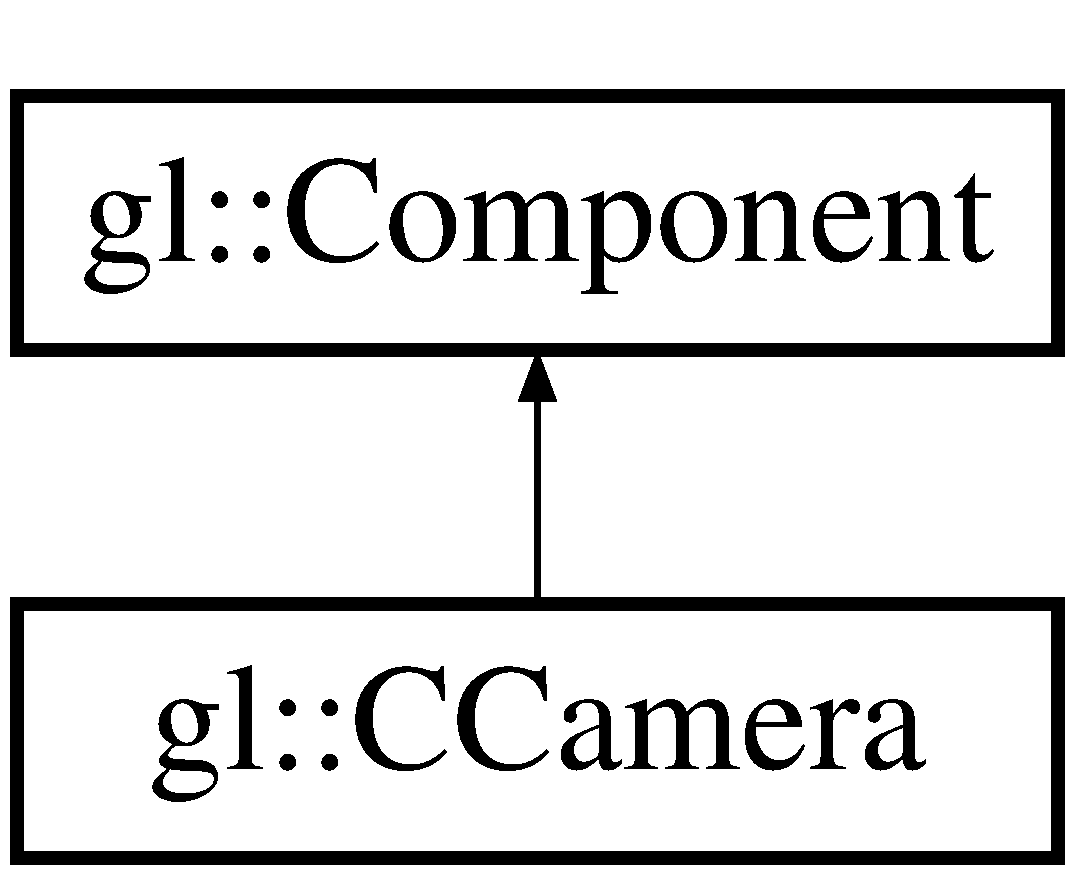
\includegraphics[height=2.000000cm]{classgl_1_1_c_camera}
\end{center}
\end{figure}
\subsection*{Public Member Functions}
\begin{DoxyCompactItemize}
\item 
\hyperlink{classgl_1_1_c_camera_aa8826c767270c515a764c4f2ee8f9379}{C\-Camera} (\hyperlink{classgl_1_1_game_object}{Game\-Object} $\ast$p\-Owner)
\item 
virtual \hyperlink{classgl_1_1_c_camera_ada23394ce1971b8de15e6dcfeda0f3b2}{$\sim$\-C\-Camera} ()
\end{DoxyCompactItemize}
\subsection*{Additional Inherited Members}


\subsection{Detailed Description}
\hyperlink{classgl_1_1_c_camera}{C\-Camera} is a \hyperlink{classgl_1_1_game_object}{Game\-Object} component that represents open\-G\-L camera. 

Definition at line 12 of file C\-Camera.\-hpp.



\subsection{Constructor \& Destructor Documentation}
\hypertarget{classgl_1_1_c_camera_aa8826c767270c515a764c4f2ee8f9379}{\index{gl\-::\-C\-Camera@{gl\-::\-C\-Camera}!C\-Camera@{C\-Camera}}
\index{C\-Camera@{C\-Camera}!gl::CCamera@{gl\-::\-C\-Camera}}
\subsubsection[{C\-Camera}]{\setlength{\rightskip}{0pt plus 5cm}gl\-::\-C\-Camera\-::\-C\-Camera (
\begin{DoxyParamCaption}
\item[{{\bf Game\-Object} $\ast$}]{p\-Owner}
\end{DoxyParamCaption}
)}}\label{classgl_1_1_c_camera_aa8826c767270c515a764c4f2ee8f9379}


Definition at line 6 of file C\-Camera.\-cpp.

\hypertarget{classgl_1_1_c_camera_ada23394ce1971b8de15e6dcfeda0f3b2}{\index{gl\-::\-C\-Camera@{gl\-::\-C\-Camera}!$\sim$\-C\-Camera@{$\sim$\-C\-Camera}}
\index{$\sim$\-C\-Camera@{$\sim$\-C\-Camera}!gl::CCamera@{gl\-::\-C\-Camera}}
\subsubsection[{$\sim$\-C\-Camera}]{\setlength{\rightskip}{0pt plus 5cm}gl\-::\-C\-Camera\-::$\sim$\-C\-Camera (
\begin{DoxyParamCaption}
{}
\end{DoxyParamCaption}
)\hspace{0.3cm}{\ttfamily [virtual]}}}\label{classgl_1_1_c_camera_ada23394ce1971b8de15e6dcfeda0f3b2}


Definition at line 13 of file C\-Camera.\-cpp.



The documentation for this class was generated from the following files\-:\begin{DoxyCompactItemize}
\item 
Glide/\hyperlink{_c_camera_8hpp}{C\-Camera.\-hpp}\item 
Glide/\hyperlink{_c_camera_8cpp}{C\-Camera.\-cpp}\end{DoxyCompactItemize}

\hypertarget{classgl_1_1_component}{\section{gl\-:\-:Component Class Reference}
\label{classgl_1_1_component}\index{gl\-::\-Component@{gl\-::\-Component}}
}


{\ttfamily \#include $<$Component.\-hpp$>$}

Inheritance diagram for gl\-:\-:Component\-:\begin{figure}[H]
\begin{center}
\leavevmode
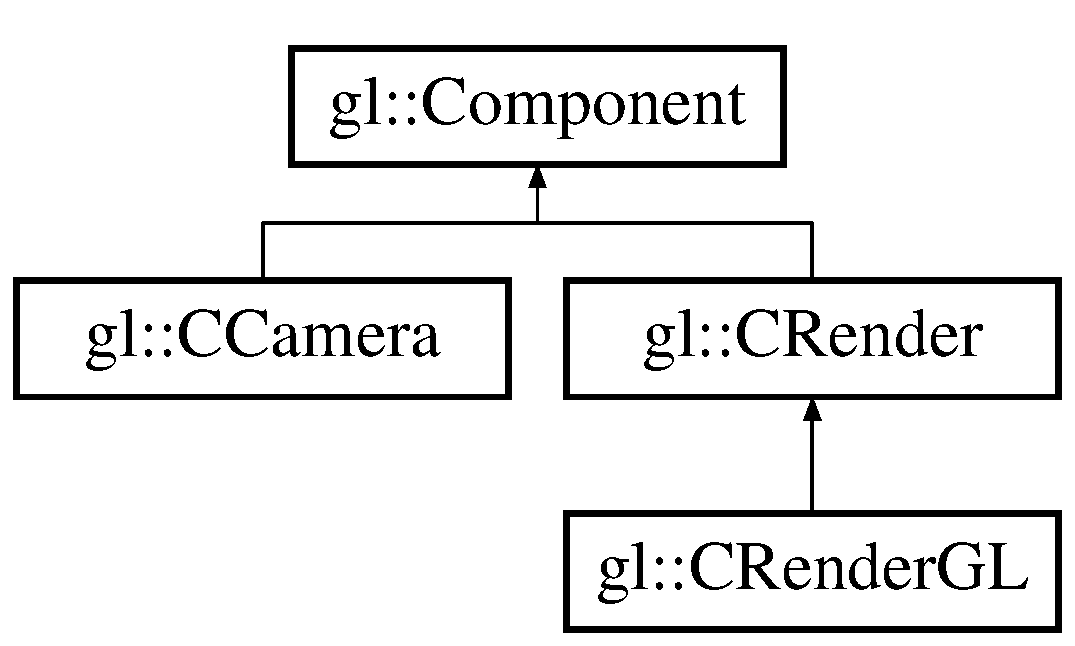
\includegraphics[height=3.000000cm]{classgl_1_1_component}
\end{center}
\end{figure}
\subsection*{Public Types}
\begin{DoxyCompactItemize}
\item 
typedef std\-::string \hyperlink{classgl_1_1_component_a55fcc946bfc525917e6380e5b71a3f49}{Family\-I\-D}
\item 
typedef std\-::string \hyperlink{classgl_1_1_component_a2dae94eddffdba218f51d19dd9d66e4e}{Type\-I\-D}
\end{DoxyCompactItemize}
\subsection*{Public Member Functions}
\begin{DoxyCompactItemize}
\item 
\hyperlink{classgl_1_1_component_a412f50df1466615614c3b62421cebbc7}{Component} (const \hyperlink{classgl_1_1_component_a55fcc946bfc525917e6380e5b71a3f49}{Family\-I\-D} \&family\-I\-D, const \hyperlink{classgl_1_1_component_a2dae94eddffdba218f51d19dd9d66e4e}{Type\-I\-D} \&type\-I\-D, \hyperlink{classgl_1_1_game_object}{Game\-Object} $\ast$p\-Owner)
\item 
\hyperlink{classgl_1_1_component_a6c651251c2ce4c2243eda34815e80d59}{Component} ()
\item 
virtual \hyperlink{classgl_1_1_component_a43f758bf7272ace3aaae840489a4a8ae}{$\sim$\-Component} ()
\item 
const \hyperlink{classgl_1_1_component_a55fcc946bfc525917e6380e5b71a3f49}{Family\-I\-D} \& \hyperlink{classgl_1_1_component_aae7441b8490f9edafb99189b937fd8a0}{Get\-Family\-I\-D} () const 
\item 
const \hyperlink{classgl_1_1_component_a2dae94eddffdba218f51d19dd9d66e4e}{Type\-I\-D} \& \hyperlink{classgl_1_1_component_a5a4746393db3e96ca12b662b7ff7ae3a}{Get\-Type\-I\-D} () const 
\item 
\hyperlink{_basic_types_8hpp_afdf0f22c576e6ee1b982f64b839c4bea}{Void} \hyperlink{classgl_1_1_component_a5583d825aaba0cfbebe199cd36948cb8}{Set\-Family\-I\-D} (const \hyperlink{classgl_1_1_component_a55fcc946bfc525917e6380e5b71a3f49}{Family\-I\-D} \&id)
\item 
\hyperlink{_basic_types_8hpp_afdf0f22c576e6ee1b982f64b839c4bea}{Void} \hyperlink{classgl_1_1_component_aba697a90e30a22386b19dc02bcb6ca58}{Set\-Type\-I\-D} (const \hyperlink{classgl_1_1_component_a2dae94eddffdba218f51d19dd9d66e4e}{Type\-I\-D} \&id)
\item 
\hyperlink{classgl_1_1_game_object}{Game\-Object} $\ast$ \hyperlink{classgl_1_1_component_a8bc9370f252fd5e9e6f7d47b5f84429b}{Get\-Owner} () const 
\item 
\hyperlink{_basic_types_8hpp_afdf0f22c576e6ee1b982f64b839c4bea}{Void} \hyperlink{classgl_1_1_component_acc20da81fa79ebeaf5bfd1d596cb2641}{Set\-Owner} (\hyperlink{classgl_1_1_game_object}{Game\-Object} $\ast$p\-Object)
\item 
virtual \hyperlink{_basic_types_8hpp_afdf0f22c576e6ee1b982f64b839c4bea}{Void} \hyperlink{classgl_1_1_component_afb18555fefa75987ff5532e874e3b3a1}{Update} ()
\end{DoxyCompactItemize}


\subsection{Detailed Description}
\hyperlink{classgl_1_1_component}{Component} is the base class for all components. 

Definition at line 16 of file Component.\-hpp.



\subsection{Member Typedef Documentation}
\hypertarget{classgl_1_1_component_a55fcc946bfc525917e6380e5b71a3f49}{\index{gl\-::\-Component@{gl\-::\-Component}!Family\-I\-D@{Family\-I\-D}}
\index{Family\-I\-D@{Family\-I\-D}!gl::Component@{gl\-::\-Component}}
\subsubsection[{Family\-I\-D}]{\setlength{\rightskip}{0pt plus 5cm}typedef std\-::string {\bf gl\-::\-Component\-::\-Family\-I\-D}}}\label{classgl_1_1_component_a55fcc946bfc525917e6380e5b71a3f49}
Every direct child of \hyperlink{classgl_1_1_component}{Component} should have a unique family id. 

Definition at line 22 of file Component.\-hpp.

\hypertarget{classgl_1_1_component_a2dae94eddffdba218f51d19dd9d66e4e}{\index{gl\-::\-Component@{gl\-::\-Component}!Type\-I\-D@{Type\-I\-D}}
\index{Type\-I\-D@{Type\-I\-D}!gl::Component@{gl\-::\-Component}}
\subsubsection[{Type\-I\-D}]{\setlength{\rightskip}{0pt plus 5cm}typedef std\-::string {\bf gl\-::\-Component\-::\-Type\-I\-D}}}\label{classgl_1_1_component_a2dae94eddffdba218f51d19dd9d66e4e}
If you need to differentiate between family components use this Type\-I\-D 

Definition at line 26 of file Component.\-hpp.



\subsection{Constructor \& Destructor Documentation}
\hypertarget{classgl_1_1_component_a412f50df1466615614c3b62421cebbc7}{\index{gl\-::\-Component@{gl\-::\-Component}!Component@{Component}}
\index{Component@{Component}!gl::Component@{gl\-::\-Component}}
\subsubsection[{Component}]{\setlength{\rightskip}{0pt plus 5cm}gl\-::\-Component\-::\-Component (
\begin{DoxyParamCaption}
\item[{const {\bf Family\-I\-D} \&}]{family\-I\-D, }
\item[{const {\bf Type\-I\-D} \&}]{type\-I\-D, }
\item[{{\bf Game\-Object} $\ast$}]{p\-Owner}
\end{DoxyParamCaption}
)}}\label{classgl_1_1_component_a412f50df1466615614c3b62421cebbc7}


Definition at line 6 of file Component.\-cpp.

\hypertarget{classgl_1_1_component_a6c651251c2ce4c2243eda34815e80d59}{\index{gl\-::\-Component@{gl\-::\-Component}!Component@{Component}}
\index{Component@{Component}!gl::Component@{gl\-::\-Component}}
\subsubsection[{Component}]{\setlength{\rightskip}{0pt plus 5cm}gl\-::\-Component\-::\-Component (
\begin{DoxyParamCaption}
{}
\end{DoxyParamCaption}
)}}\label{classgl_1_1_component_a6c651251c2ce4c2243eda34815e80d59}


Definition at line 15 of file Component.\-cpp.

\hypertarget{classgl_1_1_component_a43f758bf7272ace3aaae840489a4a8ae}{\index{gl\-::\-Component@{gl\-::\-Component}!$\sim$\-Component@{$\sim$\-Component}}
\index{$\sim$\-Component@{$\sim$\-Component}!gl::Component@{gl\-::\-Component}}
\subsubsection[{$\sim$\-Component}]{\setlength{\rightskip}{0pt plus 5cm}gl\-::\-Component\-::$\sim$\-Component (
\begin{DoxyParamCaption}
{}
\end{DoxyParamCaption}
)\hspace{0.3cm}{\ttfamily [virtual]}}}\label{classgl_1_1_component_a43f758bf7272ace3aaae840489a4a8ae}


Definition at line 22 of file Component.\-cpp.



\subsection{Member Function Documentation}
\hypertarget{classgl_1_1_component_aae7441b8490f9edafb99189b937fd8a0}{\index{gl\-::\-Component@{gl\-::\-Component}!Get\-Family\-I\-D@{Get\-Family\-I\-D}}
\index{Get\-Family\-I\-D@{Get\-Family\-I\-D}!gl::Component@{gl\-::\-Component}}
\subsubsection[{Get\-Family\-I\-D}]{\setlength{\rightskip}{0pt plus 5cm}const {\bf Component\-::\-Family\-I\-D} \& gl\-::\-Component\-::\-Get\-Family\-I\-D (
\begin{DoxyParamCaption}
{}
\end{DoxyParamCaption}
) const}}\label{classgl_1_1_component_aae7441b8490f9edafb99189b937fd8a0}
Returns the family id. 

Definition at line 26 of file Component.\-cpp.

\hypertarget{classgl_1_1_component_a8bc9370f252fd5e9e6f7d47b5f84429b}{\index{gl\-::\-Component@{gl\-::\-Component}!Get\-Owner@{Get\-Owner}}
\index{Get\-Owner@{Get\-Owner}!gl::Component@{gl\-::\-Component}}
\subsubsection[{Get\-Owner}]{\setlength{\rightskip}{0pt plus 5cm}{\bf Game\-Object} $\ast$ gl\-::\-Component\-::\-Get\-Owner (
\begin{DoxyParamCaption}
{}
\end{DoxyParamCaption}
) const}}\label{classgl_1_1_component_a8bc9370f252fd5e9e6f7d47b5f84429b}


Definition at line 46 of file Component.\-cpp.

\hypertarget{classgl_1_1_component_a5a4746393db3e96ca12b662b7ff7ae3a}{\index{gl\-::\-Component@{gl\-::\-Component}!Get\-Type\-I\-D@{Get\-Type\-I\-D}}
\index{Get\-Type\-I\-D@{Get\-Type\-I\-D}!gl::Component@{gl\-::\-Component}}
\subsubsection[{Get\-Type\-I\-D}]{\setlength{\rightskip}{0pt plus 5cm}const {\bf Component\-::\-Type\-I\-D} \& gl\-::\-Component\-::\-Get\-Type\-I\-D (
\begin{DoxyParamCaption}
{}
\end{DoxyParamCaption}
) const}}\label{classgl_1_1_component_a5a4746393db3e96ca12b662b7ff7ae3a}
returns the type id. 

Definition at line 31 of file Component.\-cpp.

\hypertarget{classgl_1_1_component_a5583d825aaba0cfbebe199cd36948cb8}{\index{gl\-::\-Component@{gl\-::\-Component}!Set\-Family\-I\-D@{Set\-Family\-I\-D}}
\index{Set\-Family\-I\-D@{Set\-Family\-I\-D}!gl::Component@{gl\-::\-Component}}
\subsubsection[{Set\-Family\-I\-D}]{\setlength{\rightskip}{0pt plus 5cm}{\bf Void} gl\-::\-Component\-::\-Set\-Family\-I\-D (
\begin{DoxyParamCaption}
\item[{const {\bf Family\-I\-D} \&}]{id}
\end{DoxyParamCaption}
)}}\label{classgl_1_1_component_a5583d825aaba0cfbebe199cd36948cb8}


Definition at line 36 of file Component.\-cpp.

\hypertarget{classgl_1_1_component_acc20da81fa79ebeaf5bfd1d596cb2641}{\index{gl\-::\-Component@{gl\-::\-Component}!Set\-Owner@{Set\-Owner}}
\index{Set\-Owner@{Set\-Owner}!gl::Component@{gl\-::\-Component}}
\subsubsection[{Set\-Owner}]{\setlength{\rightskip}{0pt plus 5cm}{\bf Void} gl\-::\-Component\-::\-Set\-Owner (
\begin{DoxyParamCaption}
\item[{{\bf Game\-Object} $\ast$}]{p\-Object}
\end{DoxyParamCaption}
)}}\label{classgl_1_1_component_acc20da81fa79ebeaf5bfd1d596cb2641}


Definition at line 51 of file Component.\-cpp.

\hypertarget{classgl_1_1_component_aba697a90e30a22386b19dc02bcb6ca58}{\index{gl\-::\-Component@{gl\-::\-Component}!Set\-Type\-I\-D@{Set\-Type\-I\-D}}
\index{Set\-Type\-I\-D@{Set\-Type\-I\-D}!gl::Component@{gl\-::\-Component}}
\subsubsection[{Set\-Type\-I\-D}]{\setlength{\rightskip}{0pt plus 5cm}{\bf Void} gl\-::\-Component\-::\-Set\-Type\-I\-D (
\begin{DoxyParamCaption}
\item[{const {\bf Type\-I\-D} \&}]{id}
\end{DoxyParamCaption}
)}}\label{classgl_1_1_component_aba697a90e30a22386b19dc02bcb6ca58}


Definition at line 41 of file Component.\-cpp.

\hypertarget{classgl_1_1_component_afb18555fefa75987ff5532e874e3b3a1}{\index{gl\-::\-Component@{gl\-::\-Component}!Update@{Update}}
\index{Update@{Update}!gl::Component@{gl\-::\-Component}}
\subsubsection[{Update}]{\setlength{\rightskip}{0pt plus 5cm}{\bf Void} gl\-::\-Component\-::\-Update (
\begin{DoxyParamCaption}
{}
\end{DoxyParamCaption}
)\hspace{0.3cm}{\ttfamily [virtual]}}}\label{classgl_1_1_component_afb18555fefa75987ff5532e874e3b3a1}
virtual call to update components. 

Definition at line 56 of file Component.\-cpp.



The documentation for this class was generated from the following files\-:\begin{DoxyCompactItemize}
\item 
Glide/\hyperlink{_component_8hpp}{Component.\-hpp}\item 
Glide/\hyperlink{_component_8cpp}{Component.\-cpp}\end{DoxyCompactItemize}

\hypertarget{classgl_1_1_r_shader_1_1_configuration}{\section{gl\-:\-:R\-Shader\-:\-:Configuration Class Reference}
\label{classgl_1_1_r_shader_1_1_configuration}\index{gl\-::\-R\-Shader\-::\-Configuration@{gl\-::\-R\-Shader\-::\-Configuration}}
}


{\ttfamily \#include $<$R\-Shader.\-hpp$>$}

Inheritance diagram for gl\-:\-:R\-Shader\-:\-:Configuration\-:\begin{figure}[H]
\begin{center}
\leavevmode
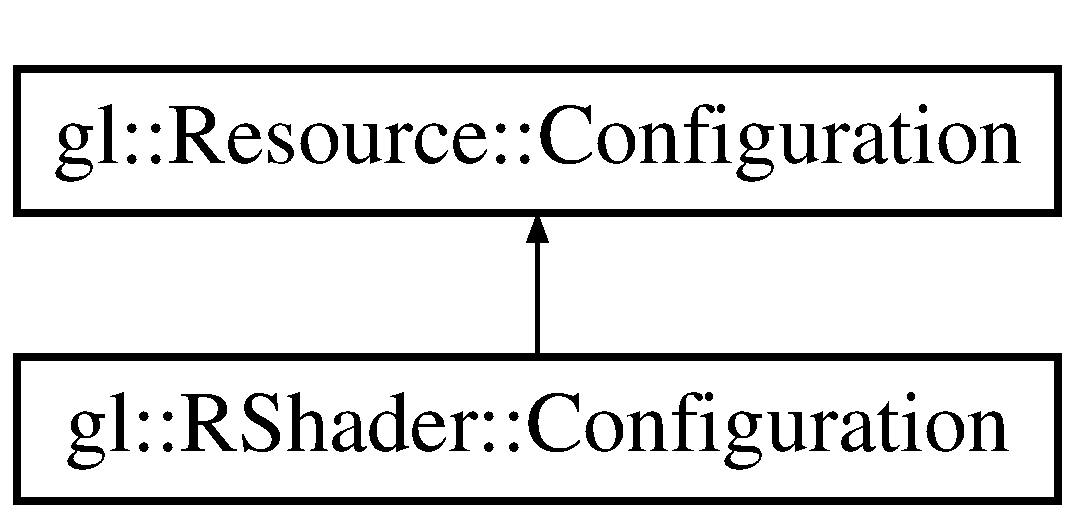
\includegraphics[height=2.000000cm]{classgl_1_1_r_shader_1_1_configuration}
\end{center}
\end{figure}
\subsection*{Public Member Functions}
\begin{DoxyCompactItemize}
\item 
\hyperlink{classgl_1_1_r_shader_1_1_configuration_ac27d7f6409dbe361012d2f705f799388}{Configuration} (const std\-::string \&vertex\-File, const std\-::string \&frag\-File)
\item 
virtual \hyperlink{classgl_1_1_r_shader_1_1_configuration_ae0a972948a97133027fff1c679f13bb3}{$\sim$\-Configuration} ()
\end{DoxyCompactItemize}
\subsection*{Public Attributes}
\begin{DoxyCompactItemize}
\item 
std\-::string \hyperlink{classgl_1_1_r_shader_1_1_configuration_aa9f93b7f474bb49fd0b94db1f77338d4}{m\-Vertex\-File}
\item 
std\-::string \hyperlink{classgl_1_1_r_shader_1_1_configuration_aa59e52a59b0a293d951c6ab1af16189a}{m\-Frag\-File}
\end{DoxyCompactItemize}
\subsection*{Additional Inherited Members}


\subsection{Detailed Description}
\hyperlink{classgl_1_1_r_shader}{R\-Shader} needs at least 2 files so we inherit from the default resource config and then add our files. 

Definition at line 64 of file R\-Shader.\-hpp.



\subsection{Constructor \& Destructor Documentation}
\hypertarget{classgl_1_1_r_shader_1_1_configuration_ac27d7f6409dbe361012d2f705f799388}{\index{gl\-::\-R\-Shader\-::\-Configuration@{gl\-::\-R\-Shader\-::\-Configuration}!Configuration@{Configuration}}
\index{Configuration@{Configuration}!gl::RShader::Configuration@{gl\-::\-R\-Shader\-::\-Configuration}}
\subsubsection[{Configuration}]{\setlength{\rightskip}{0pt plus 5cm}gl\-::\-R\-Shader\-::\-Configuration\-::\-Configuration (
\begin{DoxyParamCaption}
\item[{const std\-::string \&}]{vertex\-File, }
\item[{const std\-::string \&}]{frag\-File}
\end{DoxyParamCaption}
)}}\label{classgl_1_1_r_shader_1_1_configuration_ac27d7f6409dbe361012d2f705f799388}


Definition at line 218 of file R\-Shader.\-cpp.

\hypertarget{classgl_1_1_r_shader_1_1_configuration_ae0a972948a97133027fff1c679f13bb3}{\index{gl\-::\-R\-Shader\-::\-Configuration@{gl\-::\-R\-Shader\-::\-Configuration}!$\sim$\-Configuration@{$\sim$\-Configuration}}
\index{$\sim$\-Configuration@{$\sim$\-Configuration}!gl::RShader::Configuration@{gl\-::\-R\-Shader\-::\-Configuration}}
\subsubsection[{$\sim$\-Configuration}]{\setlength{\rightskip}{0pt plus 5cm}gl\-::\-R\-Shader\-::\-Configuration\-::$\sim$\-Configuration (
\begin{DoxyParamCaption}
{}
\end{DoxyParamCaption}
)\hspace{0.3cm}{\ttfamily [virtual]}}}\label{classgl_1_1_r_shader_1_1_configuration_ae0a972948a97133027fff1c679f13bb3}


Reimplemented from \hyperlink{classgl_1_1_resource_1_1_configuration_a4197a0f13d1481193872a7944ada4a92}{gl\-::\-Resource\-::\-Configuration}.



Definition at line 227 of file R\-Shader.\-cpp.



\subsection{Member Data Documentation}
\hypertarget{classgl_1_1_r_shader_1_1_configuration_aa59e52a59b0a293d951c6ab1af16189a}{\index{gl\-::\-R\-Shader\-::\-Configuration@{gl\-::\-R\-Shader\-::\-Configuration}!m\-Frag\-File@{m\-Frag\-File}}
\index{m\-Frag\-File@{m\-Frag\-File}!gl::RShader::Configuration@{gl\-::\-R\-Shader\-::\-Configuration}}
\subsubsection[{m\-Frag\-File}]{\setlength{\rightskip}{0pt plus 5cm}std\-::string gl\-::\-R\-Shader\-::\-Configuration\-::m\-Frag\-File}}\label{classgl_1_1_r_shader_1_1_configuration_aa59e52a59b0a293d951c6ab1af16189a}


Definition at line 71 of file R\-Shader.\-hpp.

\hypertarget{classgl_1_1_r_shader_1_1_configuration_aa9f93b7f474bb49fd0b94db1f77338d4}{\index{gl\-::\-R\-Shader\-::\-Configuration@{gl\-::\-R\-Shader\-::\-Configuration}!m\-Vertex\-File@{m\-Vertex\-File}}
\index{m\-Vertex\-File@{m\-Vertex\-File}!gl::RShader::Configuration@{gl\-::\-R\-Shader\-::\-Configuration}}
\subsubsection[{m\-Vertex\-File}]{\setlength{\rightskip}{0pt plus 5cm}std\-::string gl\-::\-R\-Shader\-::\-Configuration\-::m\-Vertex\-File}}\label{classgl_1_1_r_shader_1_1_configuration_aa9f93b7f474bb49fd0b94db1f77338d4}


Definition at line 70 of file R\-Shader.\-hpp.



The documentation for this class was generated from the following files\-:\begin{DoxyCompactItemize}
\item 
Glide/\hyperlink{_r_shader_8hpp}{R\-Shader.\-hpp}\item 
Glide/\hyperlink{_r_shader_8cpp}{R\-Shader.\-cpp}\end{DoxyCompactItemize}

\hypertarget{classgl_1_1_resource_1_1_configuration}{\section{gl\-:\-:Resource\-:\-:Configuration Class Reference}
\label{classgl_1_1_resource_1_1_configuration}\index{gl\-::\-Resource\-::\-Configuration@{gl\-::\-Resource\-::\-Configuration}}
}


{\ttfamily \#include $<$Resource\-Config.\-hpp$>$}

Inheritance diagram for gl\-:\-:Resource\-:\-:Configuration\-:\begin{figure}[H]
\begin{center}
\leavevmode
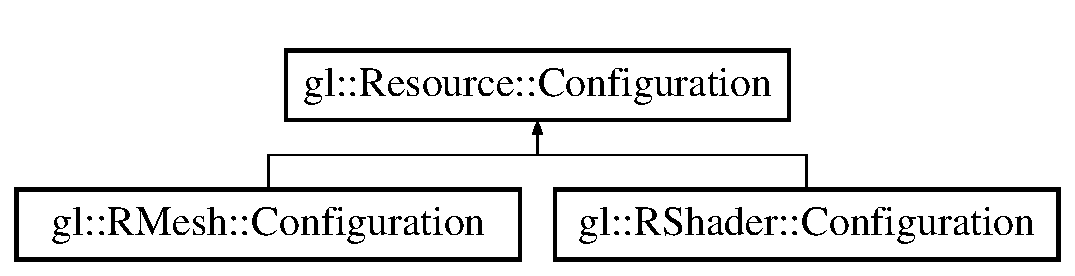
\includegraphics[height=2.000000cm]{classgl_1_1_resource_1_1_configuration}
\end{center}
\end{figure}
\subsection*{Public Member Functions}
\begin{DoxyCompactItemize}
\item 
\hyperlink{classgl_1_1_resource_1_1_configuration_a876c1175b3e2ddb5ed8333ef3ac7847f}{Configuration} (const std\-::string \&file)
\item 
virtual \hyperlink{classgl_1_1_resource_1_1_configuration_a4197a0f13d1481193872a7944ada4a92}{$\sim$\-Configuration} ()
\item 
const std\-::string \& \hyperlink{classgl_1_1_resource_1_1_configuration_a04ed41f1159b66ab65f9affe296ee977}{Get\-File\-Name\-Path} () const 
\end{DoxyCompactItemize}
\subsection*{Protected Attributes}
\begin{DoxyCompactItemize}
\item 
std\-::string \hyperlink{classgl_1_1_resource_1_1_configuration_a97e9f99cea6b131ed086e1d74bbf282e}{m\-File\-Name\-Path}
\end{DoxyCompactItemize}


\subsection{Detailed Description}
The default configuration for resources, simply takes in a file name. If you need more data in your configuration inherit from this. 

Definition at line 14 of file Resource\-Config.\-hpp.



\subsection{Constructor \& Destructor Documentation}
\hypertarget{classgl_1_1_resource_1_1_configuration_a876c1175b3e2ddb5ed8333ef3ac7847f}{\index{gl\-::\-Resource\-::\-Configuration@{gl\-::\-Resource\-::\-Configuration}!Configuration@{Configuration}}
\index{Configuration@{Configuration}!gl::Resource::Configuration@{gl\-::\-Resource\-::\-Configuration}}
\subsubsection[{Configuration}]{\setlength{\rightskip}{0pt plus 5cm}gl\-::\-Resource\-::\-Configuration\-::\-Configuration (
\begin{DoxyParamCaption}
\item[{const std\-::string \&}]{file}
\end{DoxyParamCaption}
)}}\label{classgl_1_1_resource_1_1_configuration_a876c1175b3e2ddb5ed8333ef3ac7847f}


Definition at line 6 of file Resource\-Config.\-cpp.

\hypertarget{classgl_1_1_resource_1_1_configuration_a4197a0f13d1481193872a7944ada4a92}{\index{gl\-::\-Resource\-::\-Configuration@{gl\-::\-Resource\-::\-Configuration}!$\sim$\-Configuration@{$\sim$\-Configuration}}
\index{$\sim$\-Configuration@{$\sim$\-Configuration}!gl::Resource::Configuration@{gl\-::\-Resource\-::\-Configuration}}
\subsubsection[{$\sim$\-Configuration}]{\setlength{\rightskip}{0pt plus 5cm}gl\-::\-Resource\-::\-Configuration\-::$\sim$\-Configuration (
\begin{DoxyParamCaption}
{}
\end{DoxyParamCaption}
)\hspace{0.3cm}{\ttfamily [virtual]}}}\label{classgl_1_1_resource_1_1_configuration_a4197a0f13d1481193872a7944ada4a92}


Reimplemented in \hyperlink{classgl_1_1_r_shader_1_1_configuration_ae0a972948a97133027fff1c679f13bb3}{gl\-::\-R\-Shader\-::\-Configuration}.



Definition at line 13 of file Resource\-Config.\-cpp.



\subsection{Member Function Documentation}
\hypertarget{classgl_1_1_resource_1_1_configuration_a04ed41f1159b66ab65f9affe296ee977}{\index{gl\-::\-Resource\-::\-Configuration@{gl\-::\-Resource\-::\-Configuration}!Get\-File\-Name\-Path@{Get\-File\-Name\-Path}}
\index{Get\-File\-Name\-Path@{Get\-File\-Name\-Path}!gl::Resource::Configuration@{gl\-::\-Resource\-::\-Configuration}}
\subsubsection[{Get\-File\-Name\-Path}]{\setlength{\rightskip}{0pt plus 5cm}const std\-::string \& gl\-::\-Resource\-::\-Configuration\-::\-Get\-File\-Name\-Path (
\begin{DoxyParamCaption}
{}
\end{DoxyParamCaption}
) const}}\label{classgl_1_1_resource_1_1_configuration_a04ed41f1159b66ab65f9affe296ee977}


Definition at line 18 of file Resource\-Config.\-cpp.



\subsection{Member Data Documentation}
\hypertarget{classgl_1_1_resource_1_1_configuration_a97e9f99cea6b131ed086e1d74bbf282e}{\index{gl\-::\-Resource\-::\-Configuration@{gl\-::\-Resource\-::\-Configuration}!m\-File\-Name\-Path@{m\-File\-Name\-Path}}
\index{m\-File\-Name\-Path@{m\-File\-Name\-Path}!gl::Resource::Configuration@{gl\-::\-Resource\-::\-Configuration}}
\subsubsection[{m\-File\-Name\-Path}]{\setlength{\rightskip}{0pt plus 5cm}std\-::string gl\-::\-Resource\-::\-Configuration\-::m\-File\-Name\-Path\hspace{0.3cm}{\ttfamily [protected]}}}\label{classgl_1_1_resource_1_1_configuration_a97e9f99cea6b131ed086e1d74bbf282e}


Definition at line 23 of file Resource\-Config.\-hpp.



The documentation for this class was generated from the following files\-:\begin{DoxyCompactItemize}
\item 
Glide/\hyperlink{_resource_config_8hpp}{Resource\-Config.\-hpp}\item 
Glide/\hyperlink{_resource_config_8cpp}{Resource\-Config.\-cpp}\end{DoxyCompactItemize}

\hypertarget{classgl_1_1_r_mesh_1_1_configuration}{\section{gl\-:\-:R\-Mesh\-:\-:Configuration Class Reference}
\label{classgl_1_1_r_mesh_1_1_configuration}\index{gl\-::\-R\-Mesh\-::\-Configuration@{gl\-::\-R\-Mesh\-::\-Configuration}}
}


{\ttfamily \#include $<$R\-Mesh.\-hpp$>$}

Inheritance diagram for gl\-:\-:R\-Mesh\-:\-:Configuration\-:\begin{figure}[H]
\begin{center}
\leavevmode
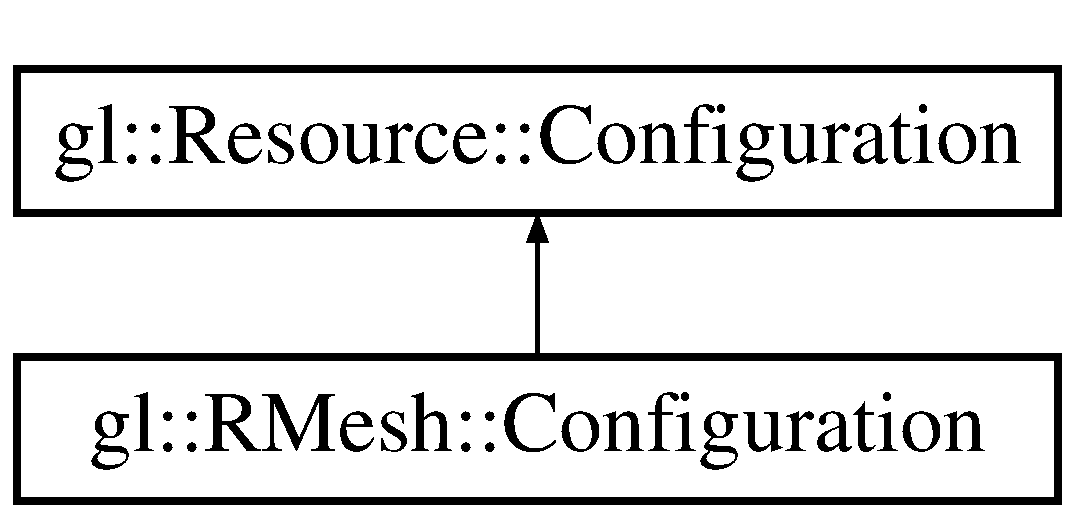
\includegraphics[height=2.000000cm]{classgl_1_1_r_mesh_1_1_configuration}
\end{center}
\end{figure}
\subsection*{Public Member Functions}
\begin{DoxyCompactItemize}
\item 
\hyperlink{classgl_1_1_r_mesh_1_1_configuration_a7df6f9974c2dbd5178d25c4a81bff7e2}{Configuration} (const std\-::string \&file, \hyperlink{classgl_1_1_r_texture}{R\-Texture} $\ast$p\-Tex, const \hyperlink{_basic_types_8hpp_a11c112f01a7ad8f767fd48bc916463a3}{U\-Int} vertex\-Count, const G\-Luint vertex\-Index\-Count, const G\-Luint vao, const G\-Luint vbo\-Positions, const G\-Luint vbo\-Normals, const G\-Luint vbo\-U\-Vs, const G\-Luint vbo\-Indices)
\end{DoxyCompactItemize}
\subsection*{Public Attributes}
\begin{DoxyCompactItemize}
\item 
\hyperlink{classgl_1_1_r_texture}{R\-Texture} $\ast$ \hyperlink{classgl_1_1_r_mesh_1_1_configuration_ab1700b1f9397d2176155d3403be81042}{mp\-Texture}
\item 
\hyperlink{_basic_types_8hpp_a11c112f01a7ad8f767fd48bc916463a3}{U\-Int} \hyperlink{classgl_1_1_r_mesh_1_1_configuration_ad3c135218126bd3aef6c177a479e6b98}{m\-Vertex\-Count}
\item 
G\-Luint \hyperlink{classgl_1_1_r_mesh_1_1_configuration_a9c44c3555d5f1b258df8fa2792750ea2}{m\-Vertex\-Index\-Count}
\item 
G\-Luint \hyperlink{classgl_1_1_r_mesh_1_1_configuration_a36cb6c53dd019a4077010f774119784f}{m\-Vao}
\item 
G\-Luint \hyperlink{classgl_1_1_r_mesh_1_1_configuration_af9085868a69ebb507797023737b341a6}{m\-Vbo\-Positions}
\item 
G\-Luint \hyperlink{classgl_1_1_r_mesh_1_1_configuration_a3e3e9308bee5e7c805a521e246bfbf01}{m\-Vbo\-Normals}
\item 
G\-Luint \hyperlink{classgl_1_1_r_mesh_1_1_configuration_a1dbf1ac4b9cf4099d7bb153cc45dac73}{m\-Vbo\-U\-Vs}
\item 
G\-Luint \hyperlink{classgl_1_1_r_mesh_1_1_configuration_a31d5227781d692261eb7404a87eb691f}{m\-Vbo\-Indices}
\end{DoxyCompactItemize}
\subsection*{Additional Inherited Members}


\subsection{Detailed Description}
\hyperlink{classgl_1_1_r_mesh}{R\-Mesh} needs more data than the default \hyperlink{classgl_1_1_resource_1_1_configuration}{Resource\-::\-Configuration} provides So we inherit from that and add our vao/vbo data ect... 

Definition at line 63 of file R\-Mesh.\-hpp.



\subsection{Constructor \& Destructor Documentation}
\hypertarget{classgl_1_1_r_mesh_1_1_configuration_a7df6f9974c2dbd5178d25c4a81bff7e2}{\index{gl\-::\-R\-Mesh\-::\-Configuration@{gl\-::\-R\-Mesh\-::\-Configuration}!Configuration@{Configuration}}
\index{Configuration@{Configuration}!gl::RMesh::Configuration@{gl\-::\-R\-Mesh\-::\-Configuration}}
\subsubsection[{Configuration}]{\setlength{\rightskip}{0pt plus 5cm}gl\-::\-R\-Mesh\-::\-Configuration\-::\-Configuration (
\begin{DoxyParamCaption}
\item[{const std\-::string \&}]{file, }
\item[{{\bf R\-Texture} $\ast$}]{p\-Tex, }
\item[{const {\bf U\-Int}}]{vertex\-Count, }
\item[{const G\-Luint}]{vertex\-Index\-Count, }
\item[{const G\-Luint}]{vao, }
\item[{const G\-Luint}]{vbo\-Positions, }
\item[{const G\-Luint}]{vbo\-Normals, }
\item[{const G\-Luint}]{vbo\-U\-Vs, }
\item[{const G\-Luint}]{vbo\-Indices}
\end{DoxyParamCaption}
)}}\label{classgl_1_1_r_mesh_1_1_configuration_a7df6f9974c2dbd5178d25c4a81bff7e2}


Definition at line 81 of file R\-Mesh.\-cpp.



\subsection{Member Data Documentation}
\hypertarget{classgl_1_1_r_mesh_1_1_configuration_ab1700b1f9397d2176155d3403be81042}{\index{gl\-::\-R\-Mesh\-::\-Configuration@{gl\-::\-R\-Mesh\-::\-Configuration}!mp\-Texture@{mp\-Texture}}
\index{mp\-Texture@{mp\-Texture}!gl::RMesh::Configuration@{gl\-::\-R\-Mesh\-::\-Configuration}}
\subsubsection[{mp\-Texture}]{\setlength{\rightskip}{0pt plus 5cm}{\bf R\-Texture}$\ast$ gl\-::\-R\-Mesh\-::\-Configuration\-::mp\-Texture}}\label{classgl_1_1_r_mesh_1_1_configuration_ab1700b1f9397d2176155d3403be81042}


Definition at line 76 of file R\-Mesh.\-hpp.

\hypertarget{classgl_1_1_r_mesh_1_1_configuration_a36cb6c53dd019a4077010f774119784f}{\index{gl\-::\-R\-Mesh\-::\-Configuration@{gl\-::\-R\-Mesh\-::\-Configuration}!m\-Vao@{m\-Vao}}
\index{m\-Vao@{m\-Vao}!gl::RMesh::Configuration@{gl\-::\-R\-Mesh\-::\-Configuration}}
\subsubsection[{m\-Vao}]{\setlength{\rightskip}{0pt plus 5cm}G\-Luint gl\-::\-R\-Mesh\-::\-Configuration\-::m\-Vao}}\label{classgl_1_1_r_mesh_1_1_configuration_a36cb6c53dd019a4077010f774119784f}


Definition at line 79 of file R\-Mesh.\-hpp.

\hypertarget{classgl_1_1_r_mesh_1_1_configuration_a31d5227781d692261eb7404a87eb691f}{\index{gl\-::\-R\-Mesh\-::\-Configuration@{gl\-::\-R\-Mesh\-::\-Configuration}!m\-Vbo\-Indices@{m\-Vbo\-Indices}}
\index{m\-Vbo\-Indices@{m\-Vbo\-Indices}!gl::RMesh::Configuration@{gl\-::\-R\-Mesh\-::\-Configuration}}
\subsubsection[{m\-Vbo\-Indices}]{\setlength{\rightskip}{0pt plus 5cm}G\-Luint gl\-::\-R\-Mesh\-::\-Configuration\-::m\-Vbo\-Indices}}\label{classgl_1_1_r_mesh_1_1_configuration_a31d5227781d692261eb7404a87eb691f}


Definition at line 83 of file R\-Mesh.\-hpp.

\hypertarget{classgl_1_1_r_mesh_1_1_configuration_a3e3e9308bee5e7c805a521e246bfbf01}{\index{gl\-::\-R\-Mesh\-::\-Configuration@{gl\-::\-R\-Mesh\-::\-Configuration}!m\-Vbo\-Normals@{m\-Vbo\-Normals}}
\index{m\-Vbo\-Normals@{m\-Vbo\-Normals}!gl::RMesh::Configuration@{gl\-::\-R\-Mesh\-::\-Configuration}}
\subsubsection[{m\-Vbo\-Normals}]{\setlength{\rightskip}{0pt plus 5cm}G\-Luint gl\-::\-R\-Mesh\-::\-Configuration\-::m\-Vbo\-Normals}}\label{classgl_1_1_r_mesh_1_1_configuration_a3e3e9308bee5e7c805a521e246bfbf01}


Definition at line 81 of file R\-Mesh.\-hpp.

\hypertarget{classgl_1_1_r_mesh_1_1_configuration_af9085868a69ebb507797023737b341a6}{\index{gl\-::\-R\-Mesh\-::\-Configuration@{gl\-::\-R\-Mesh\-::\-Configuration}!m\-Vbo\-Positions@{m\-Vbo\-Positions}}
\index{m\-Vbo\-Positions@{m\-Vbo\-Positions}!gl::RMesh::Configuration@{gl\-::\-R\-Mesh\-::\-Configuration}}
\subsubsection[{m\-Vbo\-Positions}]{\setlength{\rightskip}{0pt plus 5cm}G\-Luint gl\-::\-R\-Mesh\-::\-Configuration\-::m\-Vbo\-Positions}}\label{classgl_1_1_r_mesh_1_1_configuration_af9085868a69ebb507797023737b341a6}


Definition at line 80 of file R\-Mesh.\-hpp.

\hypertarget{classgl_1_1_r_mesh_1_1_configuration_a1dbf1ac4b9cf4099d7bb153cc45dac73}{\index{gl\-::\-R\-Mesh\-::\-Configuration@{gl\-::\-R\-Mesh\-::\-Configuration}!m\-Vbo\-U\-Vs@{m\-Vbo\-U\-Vs}}
\index{m\-Vbo\-U\-Vs@{m\-Vbo\-U\-Vs}!gl::RMesh::Configuration@{gl\-::\-R\-Mesh\-::\-Configuration}}
\subsubsection[{m\-Vbo\-U\-Vs}]{\setlength{\rightskip}{0pt plus 5cm}G\-Luint gl\-::\-R\-Mesh\-::\-Configuration\-::m\-Vbo\-U\-Vs}}\label{classgl_1_1_r_mesh_1_1_configuration_a1dbf1ac4b9cf4099d7bb153cc45dac73}


Definition at line 82 of file R\-Mesh.\-hpp.

\hypertarget{classgl_1_1_r_mesh_1_1_configuration_ad3c135218126bd3aef6c177a479e6b98}{\index{gl\-::\-R\-Mesh\-::\-Configuration@{gl\-::\-R\-Mesh\-::\-Configuration}!m\-Vertex\-Count@{m\-Vertex\-Count}}
\index{m\-Vertex\-Count@{m\-Vertex\-Count}!gl::RMesh::Configuration@{gl\-::\-R\-Mesh\-::\-Configuration}}
\subsubsection[{m\-Vertex\-Count}]{\setlength{\rightskip}{0pt plus 5cm}{\bf U\-Int} gl\-::\-R\-Mesh\-::\-Configuration\-::m\-Vertex\-Count}}\label{classgl_1_1_r_mesh_1_1_configuration_ad3c135218126bd3aef6c177a479e6b98}


Definition at line 77 of file R\-Mesh.\-hpp.

\hypertarget{classgl_1_1_r_mesh_1_1_configuration_a9c44c3555d5f1b258df8fa2792750ea2}{\index{gl\-::\-R\-Mesh\-::\-Configuration@{gl\-::\-R\-Mesh\-::\-Configuration}!m\-Vertex\-Index\-Count@{m\-Vertex\-Index\-Count}}
\index{m\-Vertex\-Index\-Count@{m\-Vertex\-Index\-Count}!gl::RMesh::Configuration@{gl\-::\-R\-Mesh\-::\-Configuration}}
\subsubsection[{m\-Vertex\-Index\-Count}]{\setlength{\rightskip}{0pt plus 5cm}G\-Luint gl\-::\-R\-Mesh\-::\-Configuration\-::m\-Vertex\-Index\-Count}}\label{classgl_1_1_r_mesh_1_1_configuration_a9c44c3555d5f1b258df8fa2792750ea2}


Definition at line 78 of file R\-Mesh.\-hpp.



The documentation for this class was generated from the following files\-:\begin{DoxyCompactItemize}
\item 
Glide/\hyperlink{_r_mesh_8hpp}{R\-Mesh.\-hpp}\item 
Glide/\hyperlink{_r_mesh_8cpp}{R\-Mesh.\-cpp}\end{DoxyCompactItemize}

\hypertarget{classgl_1_1_c_render}{\section{gl\-:\-:C\-Render Class Reference}
\label{classgl_1_1_c_render}\index{gl\-::\-C\-Render@{gl\-::\-C\-Render}}
}


{\ttfamily \#include $<$C\-Render.\-hpp$>$}

Inheritance diagram for gl\-:\-:C\-Render\-:\begin{figure}[H]
\begin{center}
\leavevmode
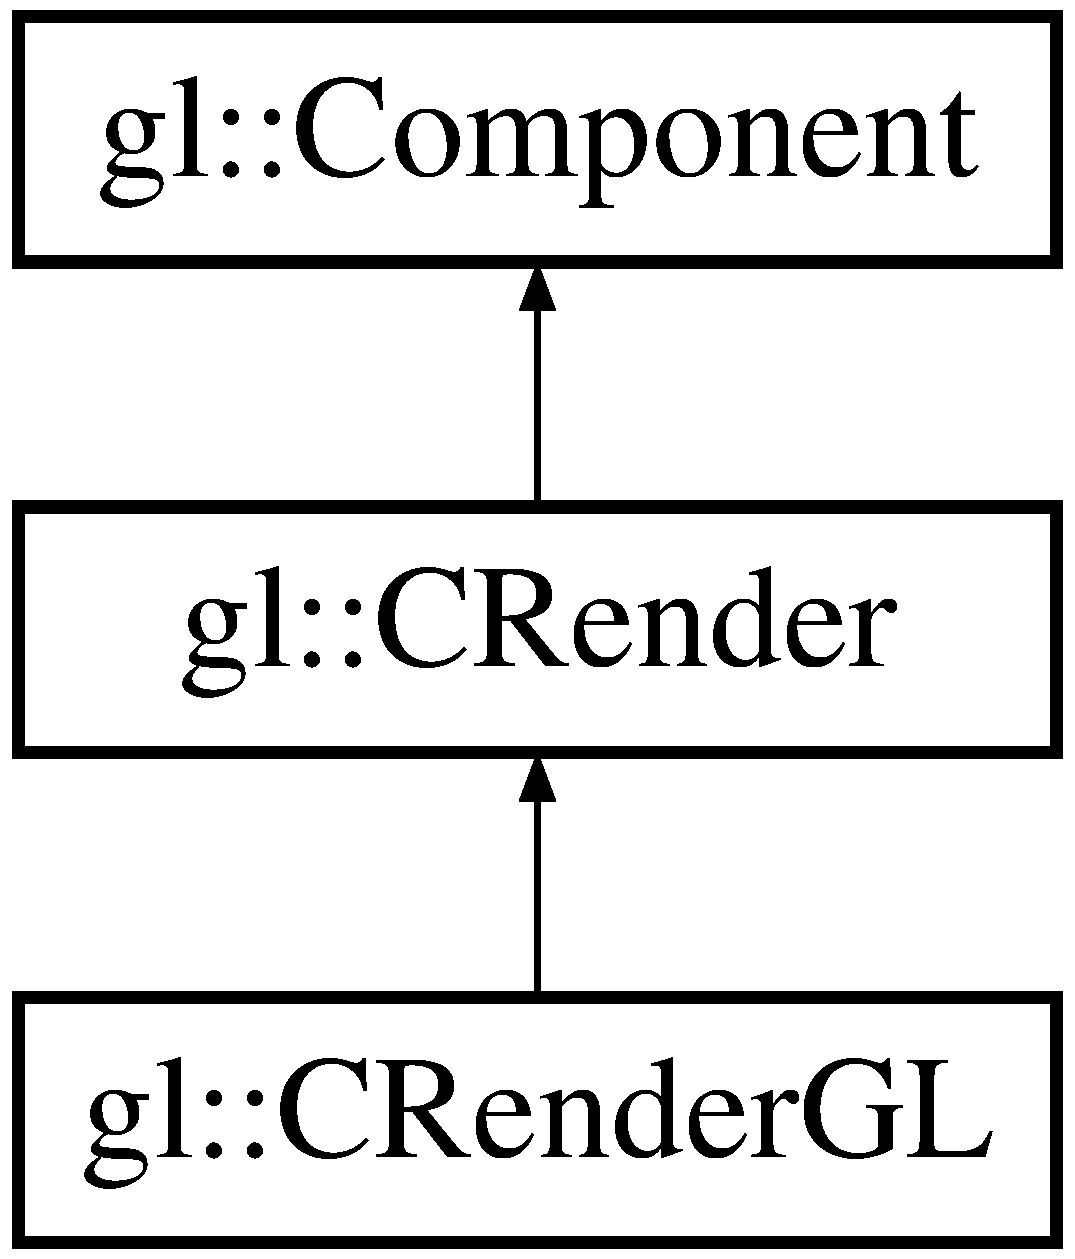
\includegraphics[height=3.000000cm]{classgl_1_1_c_render}
\end{center}
\end{figure}
\subsection*{Public Member Functions}
\begin{DoxyCompactItemize}
\item 
\hyperlink{classgl_1_1_c_render_ad81c4b1eaf7060f8314b7b63fbb35f57}{C\-Render} (const \hyperlink{classgl_1_1_component_a2dae94eddffdba218f51d19dd9d66e4e}{Type\-I\-D} \&type\-I\-D, \hyperlink{classgl_1_1_game_object}{Game\-Object} $\ast$p\-Owner, \hyperlink{classgl_1_1_r_mesh}{R\-Mesh} $\ast$p\-Mesh, \hyperlink{classgl_1_1_r_shader}{R\-Shader} $\ast$p\-Shader)
\item 
virtual \hyperlink{classgl_1_1_c_render_a28594f36d8ae3136dfd35018c0ea14a6}{$\sim$\-C\-Render} ()
\item 
virtual void \hyperlink{classgl_1_1_c_render_a9cc0ab19657613e1767fa0dd5a580617}{Render} (const glm\-::mat4 \&\hyperlink{namespacegl_a5580e107f8adbdc0f887df19caebb589}{camera})
\end{DoxyCompactItemize}
\subsection*{Protected Attributes}
\begin{DoxyCompactItemize}
\item 
\hyperlink{classgl_1_1_r_mesh}{R\-Mesh} $\ast$ \hyperlink{classgl_1_1_c_render_a0dd8e2aad391023cc6ffb31fdc84a9ba}{mp\-Mesh}
\item 
\hyperlink{classgl_1_1_r_texture}{R\-Texture} $\ast$ \hyperlink{classgl_1_1_c_render_ae6e4037e82d612aae8e25885538e96f9}{mp\-Texture}
\item 
\hyperlink{classgl_1_1_r_shader}{R\-Shader} $\ast$ \hyperlink{classgl_1_1_c_render_a7114c3d03ac0e599755f9f7f5f85960d}{mp\-Shader}
\end{DoxyCompactItemize}
\subsection*{Additional Inherited Members}


\subsection{Detailed Description}
This is the open\-G\-L Rendering component. Every \hyperlink{classgl_1_1_game_object}{Game\-Object} that needs to be rendered needs one of these. It stores the mesh, texture and shader pointers. It will grab the Texture from the mesh passed in.

N\-O\-T\-E\-: currently there is a shader pointer passed in this may change. 

Definition at line 22 of file C\-Render.\-hpp.



\subsection{Constructor \& Destructor Documentation}
\hypertarget{classgl_1_1_c_render_ad81c4b1eaf7060f8314b7b63fbb35f57}{\index{gl\-::\-C\-Render@{gl\-::\-C\-Render}!C\-Render@{C\-Render}}
\index{C\-Render@{C\-Render}!gl::CRender@{gl\-::\-C\-Render}}
\subsubsection[{C\-Render}]{\setlength{\rightskip}{0pt plus 5cm}gl\-::\-C\-Render\-::\-C\-Render (
\begin{DoxyParamCaption}
\item[{const {\bf Type\-I\-D} \&}]{type\-I\-D, }
\item[{{\bf Game\-Object} $\ast$}]{p\-Owner, }
\item[{{\bf R\-Mesh} $\ast$}]{p\-Mesh, }
\item[{{\bf R\-Shader} $\ast$}]{p\-Shader}
\end{DoxyParamCaption}
)}}\label{classgl_1_1_c_render_ad81c4b1eaf7060f8314b7b63fbb35f57}


Definition at line 12 of file C\-Render.\-cpp.

\hypertarget{classgl_1_1_c_render_a28594f36d8ae3136dfd35018c0ea14a6}{\index{gl\-::\-C\-Render@{gl\-::\-C\-Render}!$\sim$\-C\-Render@{$\sim$\-C\-Render}}
\index{$\sim$\-C\-Render@{$\sim$\-C\-Render}!gl::CRender@{gl\-::\-C\-Render}}
\subsubsection[{$\sim$\-C\-Render}]{\setlength{\rightskip}{0pt plus 5cm}gl\-::\-C\-Render\-::$\sim$\-C\-Render (
\begin{DoxyParamCaption}
{}
\end{DoxyParamCaption}
)\hspace{0.3cm}{\ttfamily [virtual]}}}\label{classgl_1_1_c_render_a28594f36d8ae3136dfd35018c0ea14a6}


Definition at line 31 of file C\-Render.\-cpp.



\subsection{Member Function Documentation}
\hypertarget{classgl_1_1_c_render_a9cc0ab19657613e1767fa0dd5a580617}{\index{gl\-::\-C\-Render@{gl\-::\-C\-Render}!Render@{Render}}
\index{Render@{Render}!gl::CRender@{gl\-::\-C\-Render}}
\subsubsection[{Render}]{\setlength{\rightskip}{0pt plus 5cm}{\bf Void} gl\-::\-C\-Render\-::\-Render (
\begin{DoxyParamCaption}
\item[{const glm\-::mat4 \&}]{camera}
\end{DoxyParamCaption}
)\hspace{0.3cm}{\ttfamily [virtual]}}}\label{classgl_1_1_c_render_a9cc0ab19657613e1767fa0dd5a580617}
render the game object this component is attached to. 

Definition at line 36 of file C\-Render.\-cpp.



\subsection{Member Data Documentation}
\hypertarget{classgl_1_1_c_render_a0dd8e2aad391023cc6ffb31fdc84a9ba}{\index{gl\-::\-C\-Render@{gl\-::\-C\-Render}!mp\-Mesh@{mp\-Mesh}}
\index{mp\-Mesh@{mp\-Mesh}!gl::CRender@{gl\-::\-C\-Render}}
\subsubsection[{mp\-Mesh}]{\setlength{\rightskip}{0pt plus 5cm}{\bf R\-Mesh}$\ast$ gl\-::\-C\-Render\-::mp\-Mesh\hspace{0.3cm}{\ttfamily [protected]}}}\label{classgl_1_1_c_render_a0dd8e2aad391023cc6ffb31fdc84a9ba}


Definition at line 35 of file C\-Render.\-hpp.

\hypertarget{classgl_1_1_c_render_a7114c3d03ac0e599755f9f7f5f85960d}{\index{gl\-::\-C\-Render@{gl\-::\-C\-Render}!mp\-Shader@{mp\-Shader}}
\index{mp\-Shader@{mp\-Shader}!gl::CRender@{gl\-::\-C\-Render}}
\subsubsection[{mp\-Shader}]{\setlength{\rightskip}{0pt plus 5cm}{\bf R\-Shader}$\ast$ gl\-::\-C\-Render\-::mp\-Shader\hspace{0.3cm}{\ttfamily [protected]}}}\label{classgl_1_1_c_render_a7114c3d03ac0e599755f9f7f5f85960d}


Definition at line 37 of file C\-Render.\-hpp.

\hypertarget{classgl_1_1_c_render_ae6e4037e82d612aae8e25885538e96f9}{\index{gl\-::\-C\-Render@{gl\-::\-C\-Render}!mp\-Texture@{mp\-Texture}}
\index{mp\-Texture@{mp\-Texture}!gl::CRender@{gl\-::\-C\-Render}}
\subsubsection[{mp\-Texture}]{\setlength{\rightskip}{0pt plus 5cm}{\bf R\-Texture}$\ast$ gl\-::\-C\-Render\-::mp\-Texture\hspace{0.3cm}{\ttfamily [protected]}}}\label{classgl_1_1_c_render_ae6e4037e82d612aae8e25885538e96f9}


Definition at line 36 of file C\-Render.\-hpp.



The documentation for this class was generated from the following files\-:\begin{DoxyCompactItemize}
\item 
Glide/\hyperlink{_c_render_8hpp}{C\-Render.\-hpp}\item 
Glide/\hyperlink{_c_render_8cpp}{C\-Render.\-cpp}\end{DoxyCompactItemize}

\hypertarget{classgl_1_1_c_render_g_l}{\section{gl\-:\-:C\-Render\-G\-L Class Reference}
\label{classgl_1_1_c_render_g_l}\index{gl\-::\-C\-Render\-G\-L@{gl\-::\-C\-Render\-G\-L}}
}


{\ttfamily \#include $<$C\-Render\-G\-L.\-hpp$>$}

Inheritance diagram for gl\-:\-:C\-Render\-G\-L\-:\begin{figure}[H]
\begin{center}
\leavevmode
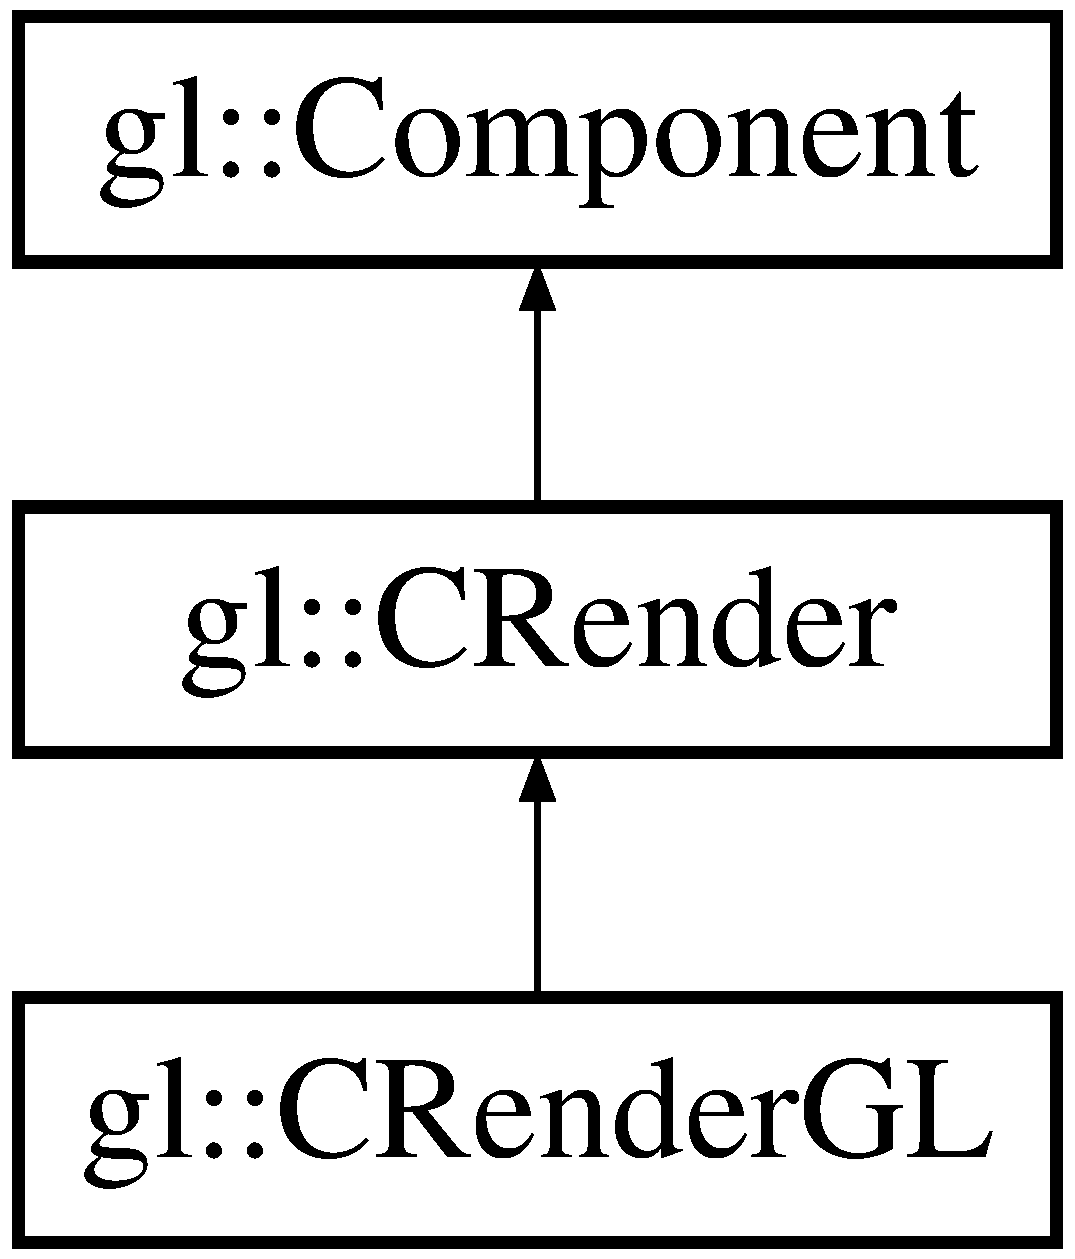
\includegraphics[height=3.000000cm]{classgl_1_1_c_render_g_l}
\end{center}
\end{figure}
\subsection*{Public Member Functions}
\begin{DoxyCompactItemize}
\item 
\hyperlink{classgl_1_1_c_render_g_l_adef34a984bce1452ec64a5e5484805c5}{C\-Render\-G\-L} (\hyperlink{classgl_1_1_game_object}{Game\-Object} $\ast$p\-Owner)
\item 
\hyperlink{classgl_1_1_c_render_g_l_a2fa95472cc459c579fd13e6b19d7ee12}{C\-Render\-G\-L} ()
\end{DoxyCompactItemize}
\subsection*{Additional Inherited Members}


\subsection{Detailed Description}
Not using this class anymore likely to be deleted some time. 

Definition at line 11 of file C\-Render\-G\-L.\-hpp.



\subsection{Constructor \& Destructor Documentation}
\hypertarget{classgl_1_1_c_render_g_l_adef34a984bce1452ec64a5e5484805c5}{\index{gl\-::\-C\-Render\-G\-L@{gl\-::\-C\-Render\-G\-L}!C\-Render\-G\-L@{C\-Render\-G\-L}}
\index{C\-Render\-G\-L@{C\-Render\-G\-L}!gl::CRenderGL@{gl\-::\-C\-Render\-G\-L}}
\subsubsection[{C\-Render\-G\-L}]{\setlength{\rightskip}{0pt plus 5cm}gl\-::\-C\-Render\-G\-L\-::\-C\-Render\-G\-L (
\begin{DoxyParamCaption}
\item[{{\bf Game\-Object} $\ast$}]{p\-Owner}
\end{DoxyParamCaption}
)}}\label{classgl_1_1_c_render_g_l_adef34a984bce1452ec64a5e5484805c5}
\hypertarget{classgl_1_1_c_render_g_l_a2fa95472cc459c579fd13e6b19d7ee12}{\index{gl\-::\-C\-Render\-G\-L@{gl\-::\-C\-Render\-G\-L}!C\-Render\-G\-L@{C\-Render\-G\-L}}
\index{C\-Render\-G\-L@{C\-Render\-G\-L}!gl::CRenderGL@{gl\-::\-C\-Render\-G\-L}}
\subsubsection[{C\-Render\-G\-L}]{\setlength{\rightskip}{0pt plus 5cm}gl\-::\-C\-Render\-G\-L\-::\-C\-Render\-G\-L (
\begin{DoxyParamCaption}
{}
\end{DoxyParamCaption}
)}}\label{classgl_1_1_c_render_g_l_a2fa95472cc459c579fd13e6b19d7ee12}


The documentation for this class was generated from the following file\-:\begin{DoxyCompactItemize}
\item 
Glide/\hyperlink{_c_render_g_l_8hpp}{C\-Render\-G\-L.\-hpp}\end{DoxyCompactItemize}

\hypertarget{classtinyxml2_1_1_dyn_array}{\section{tinyxml2\-:\-:Dyn\-Array$<$ T, I\-N\-I\-T $>$ Class Template Reference}
\label{classtinyxml2_1_1_dyn_array}\index{tinyxml2\-::\-Dyn\-Array$<$ T, I\-N\-I\-T $>$@{tinyxml2\-::\-Dyn\-Array$<$ T, I\-N\-I\-T $>$}}
}


{\ttfamily \#include $<$tinyxml2.\-hpp$>$}

\subsection*{Public Member Functions}
\begin{DoxyCompactItemize}
\item 
\hyperlink{classtinyxml2_1_1_dyn_array_af076df9203a7eda3f3501a0c84dbbb8a}{Dyn\-Array} ()
\item 
\hyperlink{classtinyxml2_1_1_dyn_array_ac7c2dc82db9010d09041ea6bfd921fdc}{$\sim$\-Dyn\-Array} ()
\item 
void \hyperlink{classtinyxml2_1_1_dyn_array_a498de53808ba0151fef54ea10bf51050}{Push} (T t)
\item 
T $\ast$ \hyperlink{classtinyxml2_1_1_dyn_array_aa3c360d40addc3b05121da9f60a01b4d}{Push\-Arr} (int count)
\item 
T \hyperlink{classtinyxml2_1_1_dyn_array_a2281e3342bc235bf391a67e362c75866}{Pop} ()
\item 
void \hyperlink{classtinyxml2_1_1_dyn_array_ab45c0836d8c0260a5b9eda7da80de71c}{Pop\-Arr} (int count)
\item 
bool \hyperlink{classtinyxml2_1_1_dyn_array_a080dc4dc68713964bb17745d4c833158}{Empty} () const 
\item 
T \& \hyperlink{classtinyxml2_1_1_dyn_array_a775a6ab4d41f0eb15bdd863d408dd58f}{operator\mbox{[}$\,$\mbox{]}} (int i)
\item 
const T \& \hyperlink{classtinyxml2_1_1_dyn_array_a1f4874c2608cbd68be1627fca9efd820}{operator\mbox{[}$\,$\mbox{]}} (int i) const 
\item 
int \hyperlink{classtinyxml2_1_1_dyn_array_a1299b257b62ea6b4983c488867f219b0}{Size} () const 
\item 
int \hyperlink{classtinyxml2_1_1_dyn_array_a8edbe90ed53b2e46b1b5cf53b261e4e7}{Capacity} () const 
\item 
const T $\ast$ \hyperlink{classtinyxml2_1_1_dyn_array_a1f39330daeb97d3d1dc3fc12dcf7ac67}{Mem} () const 
\item 
T $\ast$ \hyperlink{classtinyxml2_1_1_dyn_array_a0e0d60b399d54fad5b33d5008bc59c8e}{Mem} ()
\end{DoxyCompactItemize}


\subsection{Detailed Description}
\subsubsection*{template$<$class T, int I\-N\-I\-T$>$class tinyxml2\-::\-Dyn\-Array$<$ T, I\-N\-I\-T $>$}



Definition at line 204 of file tinyxml2.\-hpp.



\subsection{Constructor \& Destructor Documentation}
\hypertarget{classtinyxml2_1_1_dyn_array_af076df9203a7eda3f3501a0c84dbbb8a}{\index{tinyxml2\-::\-Dyn\-Array@{tinyxml2\-::\-Dyn\-Array}!Dyn\-Array@{Dyn\-Array}}
\index{Dyn\-Array@{Dyn\-Array}!tinyxml2::DynArray@{tinyxml2\-::\-Dyn\-Array}}
\subsubsection[{Dyn\-Array}]{\setlength{\rightskip}{0pt plus 5cm}template$<$class T, int I\-N\-I\-T$>$ {\bf tinyxml2\-::\-Dyn\-Array}$<$ T, I\-N\-I\-T $>$\-::{\bf Dyn\-Array} (
\begin{DoxyParamCaption}
{}
\end{DoxyParamCaption}
)\hspace{0.3cm}{\ttfamily [inline]}}}\label{classtinyxml2_1_1_dyn_array_af076df9203a7eda3f3501a0c84dbbb8a}


Definition at line 207 of file tinyxml2.\-hpp.

\hypertarget{classtinyxml2_1_1_dyn_array_ac7c2dc82db9010d09041ea6bfd921fdc}{\index{tinyxml2\-::\-Dyn\-Array@{tinyxml2\-::\-Dyn\-Array}!$\sim$\-Dyn\-Array@{$\sim$\-Dyn\-Array}}
\index{$\sim$\-Dyn\-Array@{$\sim$\-Dyn\-Array}!tinyxml2::DynArray@{tinyxml2\-::\-Dyn\-Array}}
\subsubsection[{$\sim$\-Dyn\-Array}]{\setlength{\rightskip}{0pt plus 5cm}template$<$class T, int I\-N\-I\-T$>$ {\bf tinyxml2\-::\-Dyn\-Array}$<$ T, I\-N\-I\-T $>$\-::$\sim${\bf Dyn\-Array} (
\begin{DoxyParamCaption}
{}
\end{DoxyParamCaption}
)\hspace{0.3cm}{\ttfamily [inline]}}}\label{classtinyxml2_1_1_dyn_array_ac7c2dc82db9010d09041ea6bfd921fdc}


Definition at line 213 of file tinyxml2.\-hpp.



\subsection{Member Function Documentation}
\hypertarget{classtinyxml2_1_1_dyn_array_a8edbe90ed53b2e46b1b5cf53b261e4e7}{\index{tinyxml2\-::\-Dyn\-Array@{tinyxml2\-::\-Dyn\-Array}!Capacity@{Capacity}}
\index{Capacity@{Capacity}!tinyxml2::DynArray@{tinyxml2\-::\-Dyn\-Array}}
\subsubsection[{Capacity}]{\setlength{\rightskip}{0pt plus 5cm}template$<$class T, int I\-N\-I\-T$>$ int {\bf tinyxml2\-::\-Dyn\-Array}$<$ T, I\-N\-I\-T $>$\-::Capacity (
\begin{DoxyParamCaption}
{}
\end{DoxyParamCaption}
) const\hspace{0.3cm}{\ttfamily [inline]}}}\label{classtinyxml2_1_1_dyn_array_a8edbe90ed53b2e46b1b5cf53b261e4e7}


Definition at line 258 of file tinyxml2.\-hpp.

\hypertarget{classtinyxml2_1_1_dyn_array_a080dc4dc68713964bb17745d4c833158}{\index{tinyxml2\-::\-Dyn\-Array@{tinyxml2\-::\-Dyn\-Array}!Empty@{Empty}}
\index{Empty@{Empty}!tinyxml2::DynArray@{tinyxml2\-::\-Dyn\-Array}}
\subsubsection[{Empty}]{\setlength{\rightskip}{0pt plus 5cm}template$<$class T, int I\-N\-I\-T$>$ bool {\bf tinyxml2\-::\-Dyn\-Array}$<$ T, I\-N\-I\-T $>$\-::Empty (
\begin{DoxyParamCaption}
{}
\end{DoxyParamCaption}
) const\hspace{0.3cm}{\ttfamily [inline]}}}\label{classtinyxml2_1_1_dyn_array_a080dc4dc68713964bb17745d4c833158}


Definition at line 240 of file tinyxml2.\-hpp.

\hypertarget{classtinyxml2_1_1_dyn_array_a1f39330daeb97d3d1dc3fc12dcf7ac67}{\index{tinyxml2\-::\-Dyn\-Array@{tinyxml2\-::\-Dyn\-Array}!Mem@{Mem}}
\index{Mem@{Mem}!tinyxml2::DynArray@{tinyxml2\-::\-Dyn\-Array}}
\subsubsection[{Mem}]{\setlength{\rightskip}{0pt plus 5cm}template$<$class T, int I\-N\-I\-T$>$ const T$\ast$ {\bf tinyxml2\-::\-Dyn\-Array}$<$ T, I\-N\-I\-T $>$\-::Mem (
\begin{DoxyParamCaption}
{}
\end{DoxyParamCaption}
) const\hspace{0.3cm}{\ttfamily [inline]}}}\label{classtinyxml2_1_1_dyn_array_a1f39330daeb97d3d1dc3fc12dcf7ac67}


Definition at line 262 of file tinyxml2.\-hpp.

\hypertarget{classtinyxml2_1_1_dyn_array_a0e0d60b399d54fad5b33d5008bc59c8e}{\index{tinyxml2\-::\-Dyn\-Array@{tinyxml2\-::\-Dyn\-Array}!Mem@{Mem}}
\index{Mem@{Mem}!tinyxml2::DynArray@{tinyxml2\-::\-Dyn\-Array}}
\subsubsection[{Mem}]{\setlength{\rightskip}{0pt plus 5cm}template$<$class T, int I\-N\-I\-T$>$ T$\ast$ {\bf tinyxml2\-::\-Dyn\-Array}$<$ T, I\-N\-I\-T $>$\-::Mem (
\begin{DoxyParamCaption}
{}
\end{DoxyParamCaption}
)\hspace{0.3cm}{\ttfamily [inline]}}}\label{classtinyxml2_1_1_dyn_array_a0e0d60b399d54fad5b33d5008bc59c8e}


Definition at line 266 of file tinyxml2.\-hpp.

\hypertarget{classtinyxml2_1_1_dyn_array_a775a6ab4d41f0eb15bdd863d408dd58f}{\index{tinyxml2\-::\-Dyn\-Array@{tinyxml2\-::\-Dyn\-Array}!operator\mbox{[}$\,$\mbox{]}@{operator[]}}
\index{operator\mbox{[}$\,$\mbox{]}@{operator[]}!tinyxml2::DynArray@{tinyxml2\-::\-Dyn\-Array}}
\subsubsection[{operator[]}]{\setlength{\rightskip}{0pt plus 5cm}template$<$class T, int I\-N\-I\-T$>$ T\& {\bf tinyxml2\-::\-Dyn\-Array}$<$ T, I\-N\-I\-T $>$\-::operator\mbox{[}$\,$\mbox{]} (
\begin{DoxyParamCaption}
\item[{int}]{i}
\end{DoxyParamCaption}
)\hspace{0.3cm}{\ttfamily [inline]}}}\label{classtinyxml2_1_1_dyn_array_a775a6ab4d41f0eb15bdd863d408dd58f}


Definition at line 244 of file tinyxml2.\-hpp.

\hypertarget{classtinyxml2_1_1_dyn_array_a1f4874c2608cbd68be1627fca9efd820}{\index{tinyxml2\-::\-Dyn\-Array@{tinyxml2\-::\-Dyn\-Array}!operator\mbox{[}$\,$\mbox{]}@{operator[]}}
\index{operator\mbox{[}$\,$\mbox{]}@{operator[]}!tinyxml2::DynArray@{tinyxml2\-::\-Dyn\-Array}}
\subsubsection[{operator[]}]{\setlength{\rightskip}{0pt plus 5cm}template$<$class T, int I\-N\-I\-T$>$ const T\& {\bf tinyxml2\-::\-Dyn\-Array}$<$ T, I\-N\-I\-T $>$\-::operator\mbox{[}$\,$\mbox{]} (
\begin{DoxyParamCaption}
\item[{int}]{i}
\end{DoxyParamCaption}
) const\hspace{0.3cm}{\ttfamily [inline]}}}\label{classtinyxml2_1_1_dyn_array_a1f4874c2608cbd68be1627fca9efd820}


Definition at line 249 of file tinyxml2.\-hpp.

\hypertarget{classtinyxml2_1_1_dyn_array_a2281e3342bc235bf391a67e362c75866}{\index{tinyxml2\-::\-Dyn\-Array@{tinyxml2\-::\-Dyn\-Array}!Pop@{Pop}}
\index{Pop@{Pop}!tinyxml2::DynArray@{tinyxml2\-::\-Dyn\-Array}}
\subsubsection[{Pop}]{\setlength{\rightskip}{0pt plus 5cm}template$<$class T, int I\-N\-I\-T$>$ T {\bf tinyxml2\-::\-Dyn\-Array}$<$ T, I\-N\-I\-T $>$\-::Pop (
\begin{DoxyParamCaption}
{}
\end{DoxyParamCaption}
)\hspace{0.3cm}{\ttfamily [inline]}}}\label{classtinyxml2_1_1_dyn_array_a2281e3342bc235bf391a67e362c75866}


Definition at line 231 of file tinyxml2.\-hpp.

\hypertarget{classtinyxml2_1_1_dyn_array_ab45c0836d8c0260a5b9eda7da80de71c}{\index{tinyxml2\-::\-Dyn\-Array@{tinyxml2\-::\-Dyn\-Array}!Pop\-Arr@{Pop\-Arr}}
\index{Pop\-Arr@{Pop\-Arr}!tinyxml2::DynArray@{tinyxml2\-::\-Dyn\-Array}}
\subsubsection[{Pop\-Arr}]{\setlength{\rightskip}{0pt plus 5cm}template$<$class T, int I\-N\-I\-T$>$ void {\bf tinyxml2\-::\-Dyn\-Array}$<$ T, I\-N\-I\-T $>$\-::Pop\-Arr (
\begin{DoxyParamCaption}
\item[{int}]{count}
\end{DoxyParamCaption}
)\hspace{0.3cm}{\ttfamily [inline]}}}\label{classtinyxml2_1_1_dyn_array_ab45c0836d8c0260a5b9eda7da80de71c}


Definition at line 235 of file tinyxml2.\-hpp.

\hypertarget{classtinyxml2_1_1_dyn_array_a498de53808ba0151fef54ea10bf51050}{\index{tinyxml2\-::\-Dyn\-Array@{tinyxml2\-::\-Dyn\-Array}!Push@{Push}}
\index{Push@{Push}!tinyxml2::DynArray@{tinyxml2\-::\-Dyn\-Array}}
\subsubsection[{Push}]{\setlength{\rightskip}{0pt plus 5cm}template$<$class T, int I\-N\-I\-T$>$ void {\bf tinyxml2\-::\-Dyn\-Array}$<$ T, I\-N\-I\-T $>$\-::Push (
\begin{DoxyParamCaption}
\item[{T}]{t}
\end{DoxyParamCaption}
)\hspace{0.3cm}{\ttfamily [inline]}}}\label{classtinyxml2_1_1_dyn_array_a498de53808ba0151fef54ea10bf51050}


Definition at line 219 of file tinyxml2.\-hpp.

\hypertarget{classtinyxml2_1_1_dyn_array_aa3c360d40addc3b05121da9f60a01b4d}{\index{tinyxml2\-::\-Dyn\-Array@{tinyxml2\-::\-Dyn\-Array}!Push\-Arr@{Push\-Arr}}
\index{Push\-Arr@{Push\-Arr}!tinyxml2::DynArray@{tinyxml2\-::\-Dyn\-Array}}
\subsubsection[{Push\-Arr}]{\setlength{\rightskip}{0pt plus 5cm}template$<$class T, int I\-N\-I\-T$>$ T$\ast$ {\bf tinyxml2\-::\-Dyn\-Array}$<$ T, I\-N\-I\-T $>$\-::Push\-Arr (
\begin{DoxyParamCaption}
\item[{int}]{count}
\end{DoxyParamCaption}
)\hspace{0.3cm}{\ttfamily [inline]}}}\label{classtinyxml2_1_1_dyn_array_aa3c360d40addc3b05121da9f60a01b4d}


Definition at line 224 of file tinyxml2.\-hpp.

\hypertarget{classtinyxml2_1_1_dyn_array_a1299b257b62ea6b4983c488867f219b0}{\index{tinyxml2\-::\-Dyn\-Array@{tinyxml2\-::\-Dyn\-Array}!Size@{Size}}
\index{Size@{Size}!tinyxml2::DynArray@{tinyxml2\-::\-Dyn\-Array}}
\subsubsection[{Size}]{\setlength{\rightskip}{0pt plus 5cm}template$<$class T, int I\-N\-I\-T$>$ int {\bf tinyxml2\-::\-Dyn\-Array}$<$ T, I\-N\-I\-T $>$\-::Size (
\begin{DoxyParamCaption}
{}
\end{DoxyParamCaption}
) const\hspace{0.3cm}{\ttfamily [inline]}}}\label{classtinyxml2_1_1_dyn_array_a1299b257b62ea6b4983c488867f219b0}


Definition at line 254 of file tinyxml2.\-hpp.



The documentation for this class was generated from the following file\-:\begin{DoxyCompactItemize}
\item 
Glide/\hyperlink{tinyxml2_8hpp}{tinyxml2.\-hpp}\end{DoxyCompactItemize}

\hypertarget{structtinyxml2_1_1_entity}{\section{tinyxml2\-:\-:Entity Struct Reference}
\label{structtinyxml2_1_1_entity}\index{tinyxml2\-::\-Entity@{tinyxml2\-::\-Entity}}
}
\subsection*{Public Attributes}
\begin{DoxyCompactItemize}
\item 
const char $\ast$ \hyperlink{structtinyxml2_1_1_entity_ab330f5d665d29bfc811ecfa76315894b}{pattern}
\item 
int \hyperlink{structtinyxml2_1_1_entity_a25e2b57cb59cb4fa68f283d7cb570f21}{length}
\item 
char \hyperlink{structtinyxml2_1_1_entity_a7334e81e33b4615655a403711b24f3ed}{value}
\end{DoxyCompactItemize}


\subsection{Detailed Description}


Definition at line 67 of file tinyxml2.\-cpp.



\subsection{Member Data Documentation}
\hypertarget{structtinyxml2_1_1_entity_a25e2b57cb59cb4fa68f283d7cb570f21}{\index{tinyxml2\-::\-Entity@{tinyxml2\-::\-Entity}!length@{length}}
\index{length@{length}!tinyxml2::Entity@{tinyxml2\-::\-Entity}}
\subsubsection[{length}]{\setlength{\rightskip}{0pt plus 5cm}int tinyxml2\-::\-Entity\-::length}}\label{structtinyxml2_1_1_entity_a25e2b57cb59cb4fa68f283d7cb570f21}


Definition at line 69 of file tinyxml2.\-cpp.

\hypertarget{structtinyxml2_1_1_entity_ab330f5d665d29bfc811ecfa76315894b}{\index{tinyxml2\-::\-Entity@{tinyxml2\-::\-Entity}!pattern@{pattern}}
\index{pattern@{pattern}!tinyxml2::Entity@{tinyxml2\-::\-Entity}}
\subsubsection[{pattern}]{\setlength{\rightskip}{0pt plus 5cm}const char$\ast$ tinyxml2\-::\-Entity\-::pattern}}\label{structtinyxml2_1_1_entity_ab330f5d665d29bfc811ecfa76315894b}


Definition at line 68 of file tinyxml2.\-cpp.

\hypertarget{structtinyxml2_1_1_entity_a7334e81e33b4615655a403711b24f3ed}{\index{tinyxml2\-::\-Entity@{tinyxml2\-::\-Entity}!value@{value}}
\index{value@{value}!tinyxml2::Entity@{tinyxml2\-::\-Entity}}
\subsubsection[{value}]{\setlength{\rightskip}{0pt plus 5cm}char tinyxml2\-::\-Entity\-::value}}\label{structtinyxml2_1_1_entity_a7334e81e33b4615655a403711b24f3ed}


Definition at line 70 of file tinyxml2.\-cpp.



The documentation for this struct was generated from the following file\-:\begin{DoxyCompactItemize}
\item 
Glide/\hyperlink{tinyxml2_8cpp}{tinyxml2.\-cpp}\end{DoxyCompactItemize}

\hypertarget{classgl_1_1_game_object}{\section{gl\-:\-:Game\-Object Class Reference}
\label{classgl_1_1_game_object}\index{gl\-::\-Game\-Object@{gl\-::\-Game\-Object}}
}


{\ttfamily \#include $<$Game\-Object.\-hpp$>$}

\subsection*{Public Types}
\begin{DoxyCompactItemize}
\item 
typedef std\-::string \hyperlink{classgl_1_1_game_object_af0b06465180bf63b80fe2b6d1288e4a8}{Type\-I\-D}
\end{DoxyCompactItemize}
\subsection*{Public Member Functions}
\begin{DoxyCompactItemize}
\item 
\hyperlink{classgl_1_1_game_object_a54d8bd17754619e3d7333b4fa4251b3e}{Game\-Object} (const \hyperlink{classgl_1_1_game_object_af0b06465180bf63b80fe2b6d1288e4a8}{Type\-I\-D} \&id)
\item 
\hyperlink{classgl_1_1_game_object_aa47b1c3761556efbe3c1df1639e0a588}{$\sim$\-Game\-Object} ()
\item 
\hyperlink{_basic_types_8hpp_afdf0f22c576e6ee1b982f64b839c4bea}{Void} \hyperlink{classgl_1_1_game_object_a5793cf8e0b53314435982cba0c98eebd}{Type\-I\-D\-Set} (const \hyperlink{classgl_1_1_game_object_af0b06465180bf63b80fe2b6d1288e4a8}{Type\-I\-D} \&id)
\item 
const \hyperlink{classgl_1_1_game_object_af0b06465180bf63b80fe2b6d1288e4a8}{Type\-I\-D} \& \hyperlink{classgl_1_1_game_object_a26bcf5fae15ac65b82b4f6e9a8acfe82}{Type\-I\-D\-Get} () const 
\item 
\hyperlink{classgl_1_1_game_object}{Game\-Object} $\ast$ \hyperlink{classgl_1_1_game_object_aa684ba79a38aab36ab4bea64680f3a44}{Find\-Child\-By\-I\-D} (const \hyperlink{classgl_1_1_game_object_af0b06465180bf63b80fe2b6d1288e4a8}{Type\-I\-D} \&id)
\item 
\hyperlink{_basic_types_8hpp_afdf0f22c576e6ee1b982f64b839c4bea}{Void} \hyperlink{classgl_1_1_game_object_aae16450033b01f4547bcdff6ef8fc9d9}{Component\-Add} (\hyperlink{namespacegl_a2cd59688c30d8f0b1168a93aa4bffbcc}{Component\-Ptr} \&\&p\-Comp)
\item 
\hyperlink{classgl_1_1_component}{Component} $\ast$ \hyperlink{classgl_1_1_game_object_a803ef654e89242c91d4e04b9d3907b37}{Component\-Get} (const \hyperlink{classgl_1_1_component_a55fcc946bfc525917e6380e5b71a3f49}{Component\-::\-Family\-I\-D} \&family\-I\-D)
\item 
\hyperlink{_basic_types_8hpp_afdf0f22c576e6ee1b982f64b839c4bea}{Void} \hyperlink{classgl_1_1_game_object_a4759602c4b3ec77ac88d0d1396942abc}{Calculate\-Worlds} (const glm\-::mat4 \&global\-World)
\item 
\hyperlink{_basic_types_8hpp_afdf0f22c576e6ee1b982f64b839c4bea}{Void} \hyperlink{classgl_1_1_game_object_a8556af0edf169a644fa67cc069fdc9e3}{Child\-Add} (\hyperlink{namespacegl_a4caed01d7776fc4f8768dbf8d88d0388}{Game\-Object\-Ptr} \&\&p\-Child)
\item 
\hyperlink{namespacegl_a4caed01d7776fc4f8768dbf8d88d0388}{Game\-Object\-Ptr} \&\& \hyperlink{classgl_1_1_game_object_a11ceceb648f4b90da4465d0ac0177057}{Child\-Release} (\hyperlink{classgl_1_1_game_object}{Game\-Object} $\ast$p\-Child)
\item 
\hyperlink{_basic_types_8hpp_a11c112f01a7ad8f767fd48bc916463a3}{U\-Int} \hyperlink{classgl_1_1_game_object_ac663a2b621e729dcb34a0a9e06915e26}{Child\-Count} () const 
\item 
\hyperlink{_basic_types_8hpp_afdf0f22c576e6ee1b982f64b839c4bea}{Void} \hyperlink{classgl_1_1_game_object_a470ffd663dd64d99d8e0620ee145c6be}{Set\-Parent} (\hyperlink{classgl_1_1_game_object}{Game\-Object} $\ast$p\-Parent)
\item 
glm\-::mat4 \& \hyperlink{classgl_1_1_game_object_a50205a28ddada11ebe9845a74102608d}{Get\-Local\-World} ()
\item 
const glm\-::mat4 \& \hyperlink{classgl_1_1_game_object_a5231499fc5be4d31391d91b5182aae10}{Get\-Global\-World} () const 
\item 
\hyperlink{_basic_types_8hpp_afdf0f22c576e6ee1b982f64b839c4bea}{Void} \hyperlink{classgl_1_1_game_object_a21baa7622c55cb7f517e7135aac10340}{Set\-Local\-World} (const glm\-::mat4 \&local\-World)
\item 
\hyperlink{_basic_types_8hpp_afdf0f22c576e6ee1b982f64b839c4bea}{Void} \hyperlink{classgl_1_1_game_object_a3d04c8aa54ff7ed474163d104ae8245f}{Render} (const glm\-::mat4 \&\hyperlink{namespacegl_a5580e107f8adbdc0f887df19caebb589}{camera})
\end{DoxyCompactItemize}


\subsection{Detailed Description}
\hyperlink{classgl_1_1_game_object}{Game\-Object} are the actual objects in the scene.

They are capable of Node hiarchy, and transformations too.

Game\-Objects also store Components which handle the Game\-Objects functionality and data. 

Definition at line 26 of file Game\-Object.\-hpp.



\subsection{Member Typedef Documentation}
\hypertarget{classgl_1_1_game_object_af0b06465180bf63b80fe2b6d1288e4a8}{\index{gl\-::\-Game\-Object@{gl\-::\-Game\-Object}!Type\-I\-D@{Type\-I\-D}}
\index{Type\-I\-D@{Type\-I\-D}!gl::GameObject@{gl\-::\-Game\-Object}}
\subsubsection[{Type\-I\-D}]{\setlength{\rightskip}{0pt plus 5cm}typedef std\-::string {\bf gl\-::\-Game\-Object\-::\-Type\-I\-D}}}\label{classgl_1_1_game_object_af0b06465180bf63b80fe2b6d1288e4a8}


Definition at line 29 of file Game\-Object.\-hpp.



\subsection{Constructor \& Destructor Documentation}
\hypertarget{classgl_1_1_game_object_a54d8bd17754619e3d7333b4fa4251b3e}{\index{gl\-::\-Game\-Object@{gl\-::\-Game\-Object}!Game\-Object@{Game\-Object}}
\index{Game\-Object@{Game\-Object}!gl::GameObject@{gl\-::\-Game\-Object}}
\subsubsection[{Game\-Object}]{\setlength{\rightskip}{0pt plus 5cm}gl\-::\-Game\-Object\-::\-Game\-Object (
\begin{DoxyParamCaption}
\item[{const {\bf Type\-I\-D} \&}]{id}
\end{DoxyParamCaption}
)}}\label{classgl_1_1_game_object_a54d8bd17754619e3d7333b4fa4251b3e}


Definition at line 10 of file Game\-Object.\-cpp.

\hypertarget{classgl_1_1_game_object_aa47b1c3761556efbe3c1df1639e0a588}{\index{gl\-::\-Game\-Object@{gl\-::\-Game\-Object}!$\sim$\-Game\-Object@{$\sim$\-Game\-Object}}
\index{$\sim$\-Game\-Object@{$\sim$\-Game\-Object}!gl::GameObject@{gl\-::\-Game\-Object}}
\subsubsection[{$\sim$\-Game\-Object}]{\setlength{\rightskip}{0pt plus 5cm}gl\-::\-Game\-Object\-::$\sim$\-Game\-Object (
\begin{DoxyParamCaption}
{}
\end{DoxyParamCaption}
)}}\label{classgl_1_1_game_object_aa47b1c3761556efbe3c1df1639e0a588}


Definition at line 18 of file Game\-Object.\-cpp.



\subsection{Member Function Documentation}
\hypertarget{classgl_1_1_game_object_a4759602c4b3ec77ac88d0d1396942abc}{\index{gl\-::\-Game\-Object@{gl\-::\-Game\-Object}!Calculate\-Worlds@{Calculate\-Worlds}}
\index{Calculate\-Worlds@{Calculate\-Worlds}!gl::GameObject@{gl\-::\-Game\-Object}}
\subsubsection[{Calculate\-Worlds}]{\setlength{\rightskip}{0pt plus 5cm}{\bf Void} gl\-::\-Game\-Object\-::\-Calculate\-Worlds (
\begin{DoxyParamCaption}
\item[{const glm\-::mat4 \&}]{global\-World}
\end{DoxyParamCaption}
)}}\label{classgl_1_1_game_object_a4759602c4b3ec77ac88d0d1396942abc}


Definition at line 69 of file Game\-Object.\-cpp.

\hypertarget{classgl_1_1_game_object_a8556af0edf169a644fa67cc069fdc9e3}{\index{gl\-::\-Game\-Object@{gl\-::\-Game\-Object}!Child\-Add@{Child\-Add}}
\index{Child\-Add@{Child\-Add}!gl::GameObject@{gl\-::\-Game\-Object}}
\subsubsection[{Child\-Add}]{\setlength{\rightskip}{0pt plus 5cm}{\bf Void} gl\-::\-Game\-Object\-::\-Child\-Add (
\begin{DoxyParamCaption}
\item[{{\bf Game\-Object\-Ptr} \&\&}]{p\-Child}
\end{DoxyParamCaption}
)}}\label{classgl_1_1_game_object_a8556af0edf169a644fa67cc069fdc9e3}


Definition at line 79 of file Game\-Object.\-cpp.

\hypertarget{classgl_1_1_game_object_ac663a2b621e729dcb34a0a9e06915e26}{\index{gl\-::\-Game\-Object@{gl\-::\-Game\-Object}!Child\-Count@{Child\-Count}}
\index{Child\-Count@{Child\-Count}!gl::GameObject@{gl\-::\-Game\-Object}}
\subsubsection[{Child\-Count}]{\setlength{\rightskip}{0pt plus 5cm}{\bf U\-Int} gl\-::\-Game\-Object\-::\-Child\-Count (
\begin{DoxyParamCaption}
{}
\end{DoxyParamCaption}
) const}}\label{classgl_1_1_game_object_ac663a2b621e729dcb34a0a9e06915e26}


Definition at line 108 of file Game\-Object.\-cpp.

\hypertarget{classgl_1_1_game_object_a11ceceb648f4b90da4465d0ac0177057}{\index{gl\-::\-Game\-Object@{gl\-::\-Game\-Object}!Child\-Release@{Child\-Release}}
\index{Child\-Release@{Child\-Release}!gl::GameObject@{gl\-::\-Game\-Object}}
\subsubsection[{Child\-Release}]{\setlength{\rightskip}{0pt plus 5cm}{\bf Game\-Object\-Ptr} \&\& gl\-::\-Game\-Object\-::\-Child\-Release (
\begin{DoxyParamCaption}
\item[{{\bf Game\-Object} $\ast$}]{p\-Child}
\end{DoxyParamCaption}
)}}\label{classgl_1_1_game_object_a11ceceb648f4b90da4465d0ac0177057}


Definition at line 92 of file Game\-Object.\-cpp.

\hypertarget{classgl_1_1_game_object_aae16450033b01f4547bcdff6ef8fc9d9}{\index{gl\-::\-Game\-Object@{gl\-::\-Game\-Object}!Component\-Add@{Component\-Add}}
\index{Component\-Add@{Component\-Add}!gl::GameObject@{gl\-::\-Game\-Object}}
\subsubsection[{Component\-Add}]{\setlength{\rightskip}{0pt plus 5cm}{\bf Void} gl\-::\-Game\-Object\-::\-Component\-Add (
\begin{DoxyParamCaption}
\item[{{\bf Component\-Ptr} \&\&}]{p\-Comp}
\end{DoxyParamCaption}
)}}\label{classgl_1_1_game_object_aae16450033b01f4547bcdff6ef8fc9d9}


Definition at line 49 of file Game\-Object.\-cpp.

\hypertarget{classgl_1_1_game_object_a803ef654e89242c91d4e04b9d3907b37}{\index{gl\-::\-Game\-Object@{gl\-::\-Game\-Object}!Component\-Get@{Component\-Get}}
\index{Component\-Get@{Component\-Get}!gl::GameObject@{gl\-::\-Game\-Object}}
\subsubsection[{Component\-Get}]{\setlength{\rightskip}{0pt plus 5cm}{\bf Component} $\ast$ gl\-::\-Game\-Object\-::\-Component\-Get (
\begin{DoxyParamCaption}
\item[{const {\bf Component\-::\-Family\-I\-D} \&}]{family\-I\-D}
\end{DoxyParamCaption}
)}}\label{classgl_1_1_game_object_a803ef654e89242c91d4e04b9d3907b37}


Definition at line 57 of file Game\-Object.\-cpp.

\hypertarget{classgl_1_1_game_object_aa684ba79a38aab36ab4bea64680f3a44}{\index{gl\-::\-Game\-Object@{gl\-::\-Game\-Object}!Find\-Child\-By\-I\-D@{Find\-Child\-By\-I\-D}}
\index{Find\-Child\-By\-I\-D@{Find\-Child\-By\-I\-D}!gl::GameObject@{gl\-::\-Game\-Object}}
\subsubsection[{Find\-Child\-By\-I\-D}]{\setlength{\rightskip}{0pt plus 5cm}{\bf Game\-Object} $\ast$ gl\-::\-Game\-Object\-::\-Find\-Child\-By\-I\-D (
\begin{DoxyParamCaption}
\item[{const {\bf Type\-I\-D} \&}]{id}
\end{DoxyParamCaption}
)}}\label{classgl_1_1_game_object_aa684ba79a38aab36ab4bea64680f3a44}


Definition at line 33 of file Game\-Object.\-cpp.

\hypertarget{classgl_1_1_game_object_a5231499fc5be4d31391d91b5182aae10}{\index{gl\-::\-Game\-Object@{gl\-::\-Game\-Object}!Get\-Global\-World@{Get\-Global\-World}}
\index{Get\-Global\-World@{Get\-Global\-World}!gl::GameObject@{gl\-::\-Game\-Object}}
\subsubsection[{Get\-Global\-World}]{\setlength{\rightskip}{0pt plus 5cm}const glm\-::mat4 \& gl\-::\-Game\-Object\-::\-Get\-Global\-World (
\begin{DoxyParamCaption}
{}
\end{DoxyParamCaption}
) const}}\label{classgl_1_1_game_object_a5231499fc5be4d31391d91b5182aae10}


Definition at line 123 of file Game\-Object.\-cpp.

\hypertarget{classgl_1_1_game_object_a50205a28ddada11ebe9845a74102608d}{\index{gl\-::\-Game\-Object@{gl\-::\-Game\-Object}!Get\-Local\-World@{Get\-Local\-World}}
\index{Get\-Local\-World@{Get\-Local\-World}!gl::GameObject@{gl\-::\-Game\-Object}}
\subsubsection[{Get\-Local\-World}]{\setlength{\rightskip}{0pt plus 5cm}glm\-::mat4 \& gl\-::\-Game\-Object\-::\-Get\-Local\-World (
\begin{DoxyParamCaption}
{}
\end{DoxyParamCaption}
)}}\label{classgl_1_1_game_object_a50205a28ddada11ebe9845a74102608d}


Definition at line 118 of file Game\-Object.\-cpp.

\hypertarget{classgl_1_1_game_object_a3d04c8aa54ff7ed474163d104ae8245f}{\index{gl\-::\-Game\-Object@{gl\-::\-Game\-Object}!Render@{Render}}
\index{Render@{Render}!gl::GameObject@{gl\-::\-Game\-Object}}
\subsubsection[{Render}]{\setlength{\rightskip}{0pt plus 5cm}{\bf Void} gl\-::\-Game\-Object\-::\-Render (
\begin{DoxyParamCaption}
\item[{const glm\-::mat4 \&}]{camera}
\end{DoxyParamCaption}
)}}\label{classgl_1_1_game_object_a3d04c8aa54ff7ed474163d104ae8245f}


Definition at line 133 of file Game\-Object.\-cpp.

\hypertarget{classgl_1_1_game_object_a21baa7622c55cb7f517e7135aac10340}{\index{gl\-::\-Game\-Object@{gl\-::\-Game\-Object}!Set\-Local\-World@{Set\-Local\-World}}
\index{Set\-Local\-World@{Set\-Local\-World}!gl::GameObject@{gl\-::\-Game\-Object}}
\subsubsection[{Set\-Local\-World}]{\setlength{\rightskip}{0pt plus 5cm}{\bf Void} gl\-::\-Game\-Object\-::\-Set\-Local\-World (
\begin{DoxyParamCaption}
\item[{const glm\-::mat4 \&}]{local\-World}
\end{DoxyParamCaption}
)}}\label{classgl_1_1_game_object_a21baa7622c55cb7f517e7135aac10340}


Definition at line 128 of file Game\-Object.\-cpp.

\hypertarget{classgl_1_1_game_object_a470ffd663dd64d99d8e0620ee145c6be}{\index{gl\-::\-Game\-Object@{gl\-::\-Game\-Object}!Set\-Parent@{Set\-Parent}}
\index{Set\-Parent@{Set\-Parent}!gl::GameObject@{gl\-::\-Game\-Object}}
\subsubsection[{Set\-Parent}]{\setlength{\rightskip}{0pt plus 5cm}{\bf Void} gl\-::\-Game\-Object\-::\-Set\-Parent (
\begin{DoxyParamCaption}
\item[{{\bf Game\-Object} $\ast$}]{p\-Parent}
\end{DoxyParamCaption}
)}}\label{classgl_1_1_game_object_a470ffd663dd64d99d8e0620ee145c6be}


Definition at line 113 of file Game\-Object.\-cpp.

\hypertarget{classgl_1_1_game_object_a26bcf5fae15ac65b82b4f6e9a8acfe82}{\index{gl\-::\-Game\-Object@{gl\-::\-Game\-Object}!Type\-I\-D\-Get@{Type\-I\-D\-Get}}
\index{Type\-I\-D\-Get@{Type\-I\-D\-Get}!gl::GameObject@{gl\-::\-Game\-Object}}
\subsubsection[{Type\-I\-D\-Get}]{\setlength{\rightskip}{0pt plus 5cm}const {\bf Game\-Object\-::\-Type\-I\-D} \& gl\-::\-Game\-Object\-::\-Type\-I\-D\-Get (
\begin{DoxyParamCaption}
{}
\end{DoxyParamCaption}
) const}}\label{classgl_1_1_game_object_a26bcf5fae15ac65b82b4f6e9a8acfe82}


Definition at line 28 of file Game\-Object.\-cpp.

\hypertarget{classgl_1_1_game_object_a5793cf8e0b53314435982cba0c98eebd}{\index{gl\-::\-Game\-Object@{gl\-::\-Game\-Object}!Type\-I\-D\-Set@{Type\-I\-D\-Set}}
\index{Type\-I\-D\-Set@{Type\-I\-D\-Set}!gl::GameObject@{gl\-::\-Game\-Object}}
\subsubsection[{Type\-I\-D\-Set}]{\setlength{\rightskip}{0pt plus 5cm}{\bf Void} gl\-::\-Game\-Object\-::\-Type\-I\-D\-Set (
\begin{DoxyParamCaption}
\item[{const {\bf Type\-I\-D} \&}]{id}
\end{DoxyParamCaption}
)}}\label{classgl_1_1_game_object_a5793cf8e0b53314435982cba0c98eebd}


Definition at line 23 of file Game\-Object.\-cpp.



The documentation for this class was generated from the following files\-:\begin{DoxyCompactItemize}
\item 
Glide/\hyperlink{_game_object_8hpp}{Game\-Object.\-hpp}\item 
Glide/\hyperlink{_game_object_8cpp}{Game\-Object.\-cpp}\end{DoxyCompactItemize}

\hypertarget{class_g_l_exception}{\section{G\-L\-Exception Class Reference}
\label{class_g_l_exception}\index{G\-L\-Exception@{G\-L\-Exception}}
}


The \hyperlink{class_g_l_exception}{G\-L\-Exception} class.  




{\ttfamily \#include $<$G\-L\-Check\-Error.\-hpp$>$}

Inheritance diagram for G\-L\-Exception\-:\begin{figure}[H]
\begin{center}
\leavevmode
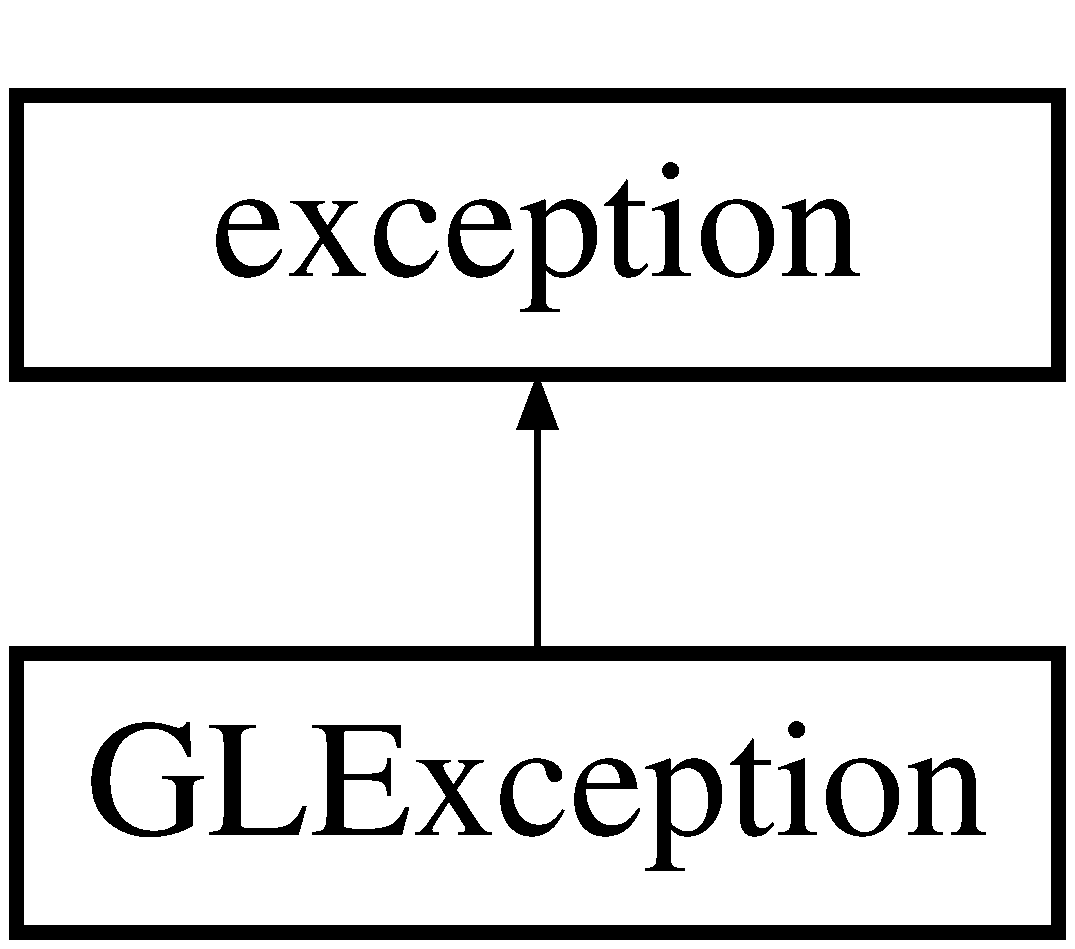
\includegraphics[height=2.000000cm]{class_g_l_exception}
\end{center}
\end{figure}
\subsection*{Public Member Functions}
\begin{DoxyCompactItemize}
\item 
\hyperlink{class_g_l_exception_a4e89f3cf9f4111c5ff27f1b4a04cbc44}{G\-L\-Exception} (int code, int line, std\-::string file)
\begin{DoxyCompactList}\small\item\em \hyperlink{class_g_l_exception}{G\-L\-Exception}. \end{DoxyCompactList}\item 
virtual const char $\ast$ \hyperlink{class_g_l_exception_adb5040f64f34f6c86e6019b0d8d65c78}{what} () const \hyperlink{_g_l_check_error_8hpp_a10a59554805ac7ce3905fd3540f98137}{N\-O\-E\-X\-C\-E\-P\-T}
\begin{DoxyCompactList}\small\item\em what \end{DoxyCompactList}\end{DoxyCompactItemize}


\subsection{Detailed Description}
The \hyperlink{class_g_l_exception}{G\-L\-Exception} class. 

This is the class to use for throwing an exception when an open\-G\-L error is detected.

It inherits from std\-::exception 

Definition at line 22 of file G\-L\-Check\-Error.\-hpp.



\subsection{Constructor \& Destructor Documentation}
\hypertarget{class_g_l_exception_a4e89f3cf9f4111c5ff27f1b4a04cbc44}{\index{G\-L\-Exception@{G\-L\-Exception}!G\-L\-Exception@{G\-L\-Exception}}
\index{G\-L\-Exception@{G\-L\-Exception}!GLException@{G\-L\-Exception}}
\subsubsection[{G\-L\-Exception}]{\setlength{\rightskip}{0pt plus 5cm}G\-L\-Exception\-::\-G\-L\-Exception (
\begin{DoxyParamCaption}
\item[{int}]{code, }
\item[{int}]{line, }
\item[{std\-::string}]{file}
\end{DoxyParamCaption}
)}}\label{class_g_l_exception_a4e89f3cf9f4111c5ff27f1b4a04cbc44}


\hyperlink{class_g_l_exception}{G\-L\-Exception}. 


\begin{DoxyParams}{Parameters}
{\em code} & The open\-G\-L error code. \\
\hline
{\em line} & The line which the error occurred. \\
\hline
{\em file} & The file which the error occurred. \\
\hline
\end{DoxyParams}


Definition at line 35 of file G\-L\-Check\-Error.\-cpp.



\subsection{Member Function Documentation}
\hypertarget{class_g_l_exception_adb5040f64f34f6c86e6019b0d8d65c78}{\index{G\-L\-Exception@{G\-L\-Exception}!what@{what}}
\index{what@{what}!GLException@{G\-L\-Exception}}
\subsubsection[{what}]{\setlength{\rightskip}{0pt plus 5cm}const char $\ast$ G\-L\-Exception\-::what (
\begin{DoxyParamCaption}
{}
\end{DoxyParamCaption}
) const\hspace{0.3cm}{\ttfamily [virtual]}}}\label{class_g_l_exception_adb5040f64f34f6c86e6019b0d8d65c78}


what 

\begin{DoxyReturn}{Returns}
The c-\/string to explain what happend. 
\end{DoxyReturn}


Definition at line 54 of file G\-L\-Check\-Error.\-cpp.



The documentation for this class was generated from the following files\-:\begin{DoxyCompactItemize}
\item 
Glide/\hyperlink{_g_l_check_error_8hpp}{G\-L\-Check\-Error.\-hpp}\item 
Glide/\hyperlink{_g_l_check_error_8cpp}{G\-L\-Check\-Error.\-cpp}\end{DoxyCompactItemize}

\hypertarget{classgl_1_1_glide_exception}{\section{gl\-:\-:Glide\-Exception Class Reference}
\label{classgl_1_1_glide_exception}\index{gl\-::\-Glide\-Exception@{gl\-::\-Glide\-Exception}}
}


{\ttfamily \#include $<$Glide\-Exception.\-hpp$>$}

Inheritance diagram for gl\-:\-:Glide\-Exception\-:\begin{figure}[H]
\begin{center}
\leavevmode
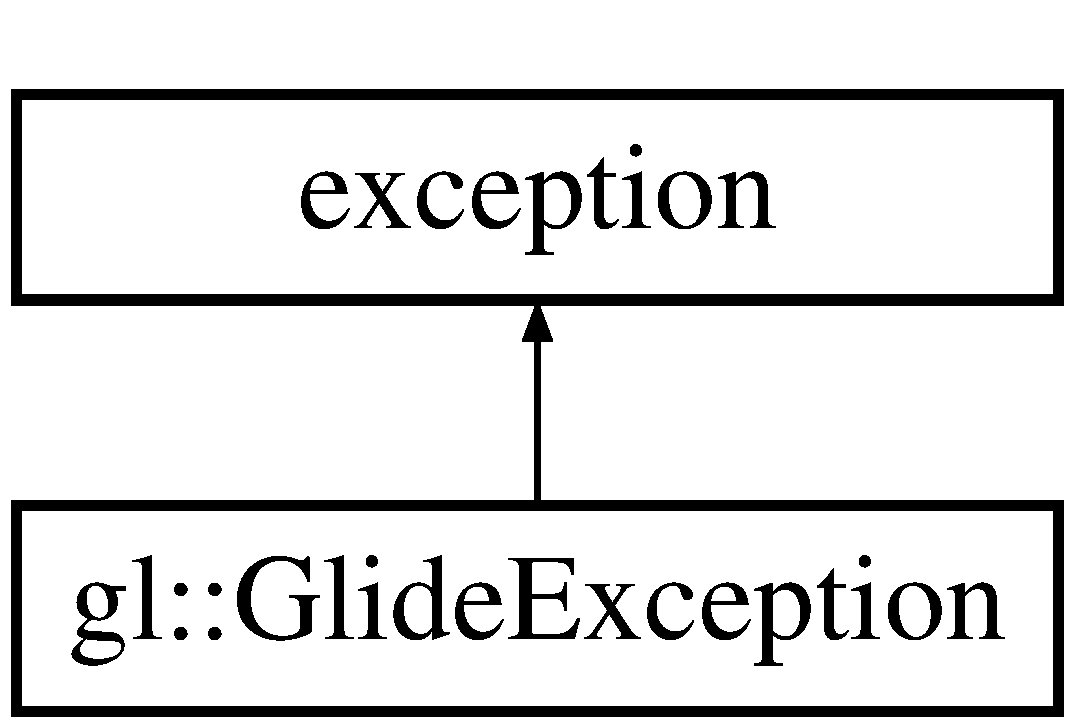
\includegraphics[height=2.000000cm]{classgl_1_1_glide_exception}
\end{center}
\end{figure}
\subsection*{Public Member Functions}
\begin{DoxyCompactItemize}
\item 
\hyperlink{classgl_1_1_glide_exception_aced3eebf8bbc7c3ece421aba2968eb08}{Glide\-Exception} (const std\-::string \&message)
\item 
\hyperlink{classgl_1_1_glide_exception_aeb51efa7265ec37545424eb14210348e}{Glide\-Exception} (const std\-::string \&message, \hyperlink{_basic_types_8hpp_a57ba1b89723b1138a6c560e57422acd5}{Long} code)
\item 
\hyperlink{classgl_1_1_glide_exception_a48c8b727d59aacc363f288f12fb178bb}{Glide\-Exception} (const std\-::string \&message, \hyperlink{_basic_types_8hpp_a57ba1b89723b1138a6c560e57422acd5}{Long} code, const std\-::string \&code\-Str)
\item 
virtual const char $\ast$ \hyperlink{classgl_1_1_glide_exception_a2c36fecffc35bb3c223a85b59f5322fe}{what} () const 
\end{DoxyCompactItemize}
\subsection*{Protected Member Functions}
\begin{DoxyCompactItemize}
\item 
\hyperlink{_basic_types_8hpp_afdf0f22c576e6ee1b982f64b839c4bea}{Void} \hyperlink{classgl_1_1_glide_exception_aef61dcf7d8844dff478b7be0e762914f}{Build\-Message} (const std\-::string \&message)
\item 
\hyperlink{_basic_types_8hpp_afdf0f22c576e6ee1b982f64b839c4bea}{Void} \hyperlink{classgl_1_1_glide_exception_a3a7e5acc5f75f29da43430ff39f8d5c4}{Build\-Message\-\_\-\-Code} (const std\-::string \&message, \hyperlink{_basic_types_8hpp_a57ba1b89723b1138a6c560e57422acd5}{Long} code)
\item 
\hyperlink{_basic_types_8hpp_afdf0f22c576e6ee1b982f64b839c4bea}{Void} \hyperlink{classgl_1_1_glide_exception_ac3327c44f3918052e70c05e7051903d2}{Build\-Message\-\_\-\-Code\-\_\-\-Code\-Str} (const std\-::string \&message, \hyperlink{_basic_types_8hpp_a57ba1b89723b1138a6c560e57422acd5}{Long} code, const std\-::string \&error\-Code\-Str)
\end{DoxyCompactItemize}
\subsection*{Protected Attributes}
\begin{DoxyCompactItemize}
\item 
std\-::string \hyperlink{classgl_1_1_glide_exception_afb68bf6b714e824ce58bef03f4264b91}{m\-What}
\end{DoxyCompactItemize}


\subsection{Detailed Description}
Use this to throw exceptions, it is std\-::except compatable.

Any time this is throw the data is also wrote to the g\-Logger. 

Definition at line 16 of file Glide\-Exception.\-hpp.



\subsection{Constructor \& Destructor Documentation}
\hypertarget{classgl_1_1_glide_exception_aced3eebf8bbc7c3ece421aba2968eb08}{\index{gl\-::\-Glide\-Exception@{gl\-::\-Glide\-Exception}!Glide\-Exception@{Glide\-Exception}}
\index{Glide\-Exception@{Glide\-Exception}!gl::GlideException@{gl\-::\-Glide\-Exception}}
\subsubsection[{Glide\-Exception}]{\setlength{\rightskip}{0pt plus 5cm}gl\-::\-Glide\-Exception\-::\-Glide\-Exception (
\begin{DoxyParamCaption}
\item[{const std\-::string \&}]{message}
\end{DoxyParamCaption}
)}}\label{classgl_1_1_glide_exception_aced3eebf8bbc7c3ece421aba2968eb08}


Definition at line 9 of file Glide\-Exception.\-cpp.

\hypertarget{classgl_1_1_glide_exception_aeb51efa7265ec37545424eb14210348e}{\index{gl\-::\-Glide\-Exception@{gl\-::\-Glide\-Exception}!Glide\-Exception@{Glide\-Exception}}
\index{Glide\-Exception@{Glide\-Exception}!gl::GlideException@{gl\-::\-Glide\-Exception}}
\subsubsection[{Glide\-Exception}]{\setlength{\rightskip}{0pt plus 5cm}gl\-::\-Glide\-Exception\-::\-Glide\-Exception (
\begin{DoxyParamCaption}
\item[{const std\-::string \&}]{message, }
\item[{{\bf Long}}]{code}
\end{DoxyParamCaption}
)}}\label{classgl_1_1_glide_exception_aeb51efa7265ec37545424eb14210348e}


Definition at line 18 of file Glide\-Exception.\-cpp.

\hypertarget{classgl_1_1_glide_exception_a48c8b727d59aacc363f288f12fb178bb}{\index{gl\-::\-Glide\-Exception@{gl\-::\-Glide\-Exception}!Glide\-Exception@{Glide\-Exception}}
\index{Glide\-Exception@{Glide\-Exception}!gl::GlideException@{gl\-::\-Glide\-Exception}}
\subsubsection[{Glide\-Exception}]{\setlength{\rightskip}{0pt plus 5cm}gl\-::\-Glide\-Exception\-::\-Glide\-Exception (
\begin{DoxyParamCaption}
\item[{const std\-::string \&}]{message, }
\item[{{\bf Long}}]{code, }
\item[{const std\-::string \&}]{code\-Str}
\end{DoxyParamCaption}
)}}\label{classgl_1_1_glide_exception_a48c8b727d59aacc363f288f12fb178bb}


Definition at line 28 of file Glide\-Exception.\-cpp.



\subsection{Member Function Documentation}
\hypertarget{classgl_1_1_glide_exception_aef61dcf7d8844dff478b7be0e762914f}{\index{gl\-::\-Glide\-Exception@{gl\-::\-Glide\-Exception}!Build\-Message@{Build\-Message}}
\index{Build\-Message@{Build\-Message}!gl::GlideException@{gl\-::\-Glide\-Exception}}
\subsubsection[{Build\-Message}]{\setlength{\rightskip}{0pt plus 5cm}{\bf Void} gl\-::\-Glide\-Exception\-::\-Build\-Message (
\begin{DoxyParamCaption}
\item[{const std\-::string \&}]{message}
\end{DoxyParamCaption}
)\hspace{0.3cm}{\ttfamily [protected]}}}\label{classgl_1_1_glide_exception_aef61dcf7d8844dff478b7be0e762914f}


Definition at line 38 of file Glide\-Exception.\-cpp.

\hypertarget{classgl_1_1_glide_exception_a3a7e5acc5f75f29da43430ff39f8d5c4}{\index{gl\-::\-Glide\-Exception@{gl\-::\-Glide\-Exception}!Build\-Message\-\_\-\-Code@{Build\-Message\-\_\-\-Code}}
\index{Build\-Message\-\_\-\-Code@{Build\-Message\-\_\-\-Code}!gl::GlideException@{gl\-::\-Glide\-Exception}}
\subsubsection[{Build\-Message\-\_\-\-Code}]{\setlength{\rightskip}{0pt plus 5cm}{\bf Void} gl\-::\-Glide\-Exception\-::\-Build\-Message\-\_\-\-Code (
\begin{DoxyParamCaption}
\item[{const std\-::string \&}]{message, }
\item[{{\bf Long}}]{code}
\end{DoxyParamCaption}
)\hspace{0.3cm}{\ttfamily [protected]}}}\label{classgl_1_1_glide_exception_a3a7e5acc5f75f29da43430ff39f8d5c4}


Definition at line 45 of file Glide\-Exception.\-cpp.

\hypertarget{classgl_1_1_glide_exception_ac3327c44f3918052e70c05e7051903d2}{\index{gl\-::\-Glide\-Exception@{gl\-::\-Glide\-Exception}!Build\-Message\-\_\-\-Code\-\_\-\-Code\-Str@{Build\-Message\-\_\-\-Code\-\_\-\-Code\-Str}}
\index{Build\-Message\-\_\-\-Code\-\_\-\-Code\-Str@{Build\-Message\-\_\-\-Code\-\_\-\-Code\-Str}!gl::GlideException@{gl\-::\-Glide\-Exception}}
\subsubsection[{Build\-Message\-\_\-\-Code\-\_\-\-Code\-Str}]{\setlength{\rightskip}{0pt plus 5cm}{\bf Void} gl\-::\-Glide\-Exception\-::\-Build\-Message\-\_\-\-Code\-\_\-\-Code\-Str (
\begin{DoxyParamCaption}
\item[{const std\-::string \&}]{message, }
\item[{{\bf Long}}]{code, }
\item[{const std\-::string \&}]{error\-Code\-Str}
\end{DoxyParamCaption}
)\hspace{0.3cm}{\ttfamily [protected]}}}\label{classgl_1_1_glide_exception_ac3327c44f3918052e70c05e7051903d2}


Definition at line 53 of file Glide\-Exception.\-cpp.

\hypertarget{classgl_1_1_glide_exception_a2c36fecffc35bb3c223a85b59f5322fe}{\index{gl\-::\-Glide\-Exception@{gl\-::\-Glide\-Exception}!what@{what}}
\index{what@{what}!gl::GlideException@{gl\-::\-Glide\-Exception}}
\subsubsection[{what}]{\setlength{\rightskip}{0pt plus 5cm}const char $\ast$ gl\-::\-Glide\-Exception\-::what (
\begin{DoxyParamCaption}
{}
\end{DoxyParamCaption}
) const\hspace{0.3cm}{\ttfamily [virtual]}}}\label{classgl_1_1_glide_exception_a2c36fecffc35bb3c223a85b59f5322fe}


Definition at line 61 of file Glide\-Exception.\-cpp.



\subsection{Member Data Documentation}
\hypertarget{classgl_1_1_glide_exception_afb68bf6b714e824ce58bef03f4264b91}{\index{gl\-::\-Glide\-Exception@{gl\-::\-Glide\-Exception}!m\-What@{m\-What}}
\index{m\-What@{m\-What}!gl::GlideException@{gl\-::\-Glide\-Exception}}
\subsubsection[{m\-What}]{\setlength{\rightskip}{0pt plus 5cm}std\-::string gl\-::\-Glide\-Exception\-::m\-What\hspace{0.3cm}{\ttfamily [protected]}}}\label{classgl_1_1_glide_exception_afb68bf6b714e824ce58bef03f4264b91}


Definition at line 30 of file Glide\-Exception.\-hpp.



The documentation for this class was generated from the following files\-:\begin{DoxyCompactItemize}
\item 
Glide/\hyperlink{_glide_exception_8hpp}{Glide\-Exception.\-hpp}\item 
Glide/\hyperlink{_glide_exception_8cpp}{Glide\-Exception.\-cpp}\end{DoxyCompactItemize}

\hypertarget{classgl_1_1_graphics_manager}{\section{gl\-:\-:Graphics\-Manager Class Reference}
\label{classgl_1_1_graphics_manager}\index{gl\-::\-Graphics\-Manager@{gl\-::\-Graphics\-Manager}}
}


{\ttfamily \#include $<$Graphics\-Manager.\-hpp$>$}

\subsection*{Public Member Functions}
\begin{DoxyCompactItemize}
\item 
\hyperlink{classgl_1_1_graphics_manager_a3ac6586fec61361f71fc6874387e62cb}{Graphics\-Manager} ()
\item 
\hyperlink{classgl_1_1_graphics_manager_a918fd5f89641e57335af2cc584ef19dd}{$\sim$\-Graphics\-Manager} ()
\item 
\hyperlink{_basic_types_8hpp_a76a8b016e5ad61faf9062cc387df5016}{Bool} \hyperlink{classgl_1_1_graphics_manager_a26f6eb89ac3df56c7ef442f255bf1f2a}{Window\-Open} () const 
\item 
\hyperlink{_basic_types_8hpp_afdf0f22c576e6ee1b982f64b839c4bea}{Void} \hyperlink{classgl_1_1_graphics_manager_ac8d6fd33d451289b908f8e3643591c59}{Update} ()
\end{DoxyCompactItemize}
\subsection*{Public Attributes}
\begin{DoxyCompactItemize}
\item 
G\-L\-F\-Wwindow $\ast$ \hyperlink{classgl_1_1_graphics_manager_a52a5220a1ae3beeefbce6303df4edd73}{mp\-Window}
\end{DoxyCompactItemize}


\subsection{Detailed Description}
Initializes glfw window and context, followed by glew to get the open\-G\-L function pointers. 

Definition at line 14 of file Graphics\-Manager.\-hpp.



\subsection{Constructor \& Destructor Documentation}
\hypertarget{classgl_1_1_graphics_manager_a3ac6586fec61361f71fc6874387e62cb}{\index{gl\-::\-Graphics\-Manager@{gl\-::\-Graphics\-Manager}!Graphics\-Manager@{Graphics\-Manager}}
\index{Graphics\-Manager@{Graphics\-Manager}!gl::GraphicsManager@{gl\-::\-Graphics\-Manager}}
\subsubsection[{Graphics\-Manager}]{\setlength{\rightskip}{0pt plus 5cm}gl\-::\-Graphics\-Manager\-::\-Graphics\-Manager (
\begin{DoxyParamCaption}
{}
\end{DoxyParamCaption}
)}}\label{classgl_1_1_graphics_manager_a3ac6586fec61361f71fc6874387e62cb}


Definition at line 21 of file Graphics\-Manager.\-cpp.

\hypertarget{classgl_1_1_graphics_manager_a918fd5f89641e57335af2cc584ef19dd}{\index{gl\-::\-Graphics\-Manager@{gl\-::\-Graphics\-Manager}!$\sim$\-Graphics\-Manager@{$\sim$\-Graphics\-Manager}}
\index{$\sim$\-Graphics\-Manager@{$\sim$\-Graphics\-Manager}!gl::GraphicsManager@{gl\-::\-Graphics\-Manager}}
\subsubsection[{$\sim$\-Graphics\-Manager}]{\setlength{\rightskip}{0pt plus 5cm}gl\-::\-Graphics\-Manager\-::$\sim$\-Graphics\-Manager (
\begin{DoxyParamCaption}
{}
\end{DoxyParamCaption}
)}}\label{classgl_1_1_graphics_manager_a918fd5f89641e57335af2cc584ef19dd}


Definition at line 99 of file Graphics\-Manager.\-cpp.



\subsection{Member Function Documentation}
\hypertarget{classgl_1_1_graphics_manager_ac8d6fd33d451289b908f8e3643591c59}{\index{gl\-::\-Graphics\-Manager@{gl\-::\-Graphics\-Manager}!Update@{Update}}
\index{Update@{Update}!gl::GraphicsManager@{gl\-::\-Graphics\-Manager}}
\subsubsection[{Update}]{\setlength{\rightskip}{0pt plus 5cm}{\bf Void} gl\-::\-Graphics\-Manager\-::\-Update (
\begin{DoxyParamCaption}
{}
\end{DoxyParamCaption}
)}}\label{classgl_1_1_graphics_manager_ac8d6fd33d451289b908f8e3643591c59}
This needs to be called every frame usually at the end of the main loop. 

Definition at line 110 of file Graphics\-Manager.\-cpp.

\hypertarget{classgl_1_1_graphics_manager_a26f6eb89ac3df56c7ef442f255bf1f2a}{\index{gl\-::\-Graphics\-Manager@{gl\-::\-Graphics\-Manager}!Window\-Open@{Window\-Open}}
\index{Window\-Open@{Window\-Open}!gl::GraphicsManager@{gl\-::\-Graphics\-Manager}}
\subsubsection[{Window\-Open}]{\setlength{\rightskip}{0pt plus 5cm}{\bf Bool} gl\-::\-Graphics\-Manager\-::\-Window\-Open (
\begin{DoxyParamCaption}
{}
\end{DoxyParamCaption}
) const}}\label{classgl_1_1_graphics_manager_a26f6eb89ac3df56c7ef442f255bf1f2a}
if this should return false the application should exit the main loop and return. 

Definition at line 105 of file Graphics\-Manager.\-cpp.



\subsection{Member Data Documentation}
\hypertarget{classgl_1_1_graphics_manager_a52a5220a1ae3beeefbce6303df4edd73}{\index{gl\-::\-Graphics\-Manager@{gl\-::\-Graphics\-Manager}!mp\-Window@{mp\-Window}}
\index{mp\-Window@{mp\-Window}!gl::GraphicsManager@{gl\-::\-Graphics\-Manager}}
\subsubsection[{mp\-Window}]{\setlength{\rightskip}{0pt plus 5cm}G\-L\-F\-Wwindow$\ast$ gl\-::\-Graphics\-Manager\-::mp\-Window}}\label{classgl_1_1_graphics_manager_a52a5220a1ae3beeefbce6303df4edd73}


Definition at line 31 of file Graphics\-Manager.\-hpp.



The documentation for this class was generated from the following files\-:\begin{DoxyCompactItemize}
\item 
Glide/\hyperlink{_graphics_manager_8hpp}{Graphics\-Manager.\-hpp}\item 
Glide/\hyperlink{_graphics_manager_8cpp}{Graphics\-Manager.\-cpp}\end{DoxyCompactItemize}

\hypertarget{classgl_1_1_logger}{\section{gl\-:\-:Logger Class Reference}
\label{classgl_1_1_logger}\index{gl\-::\-Logger@{gl\-::\-Logger}}
}


{\ttfamily \#include $<$Logger.\-hpp$>$}

Inheritance diagram for gl\-:\-:Logger\-:\begin{figure}[H]
\begin{center}
\leavevmode
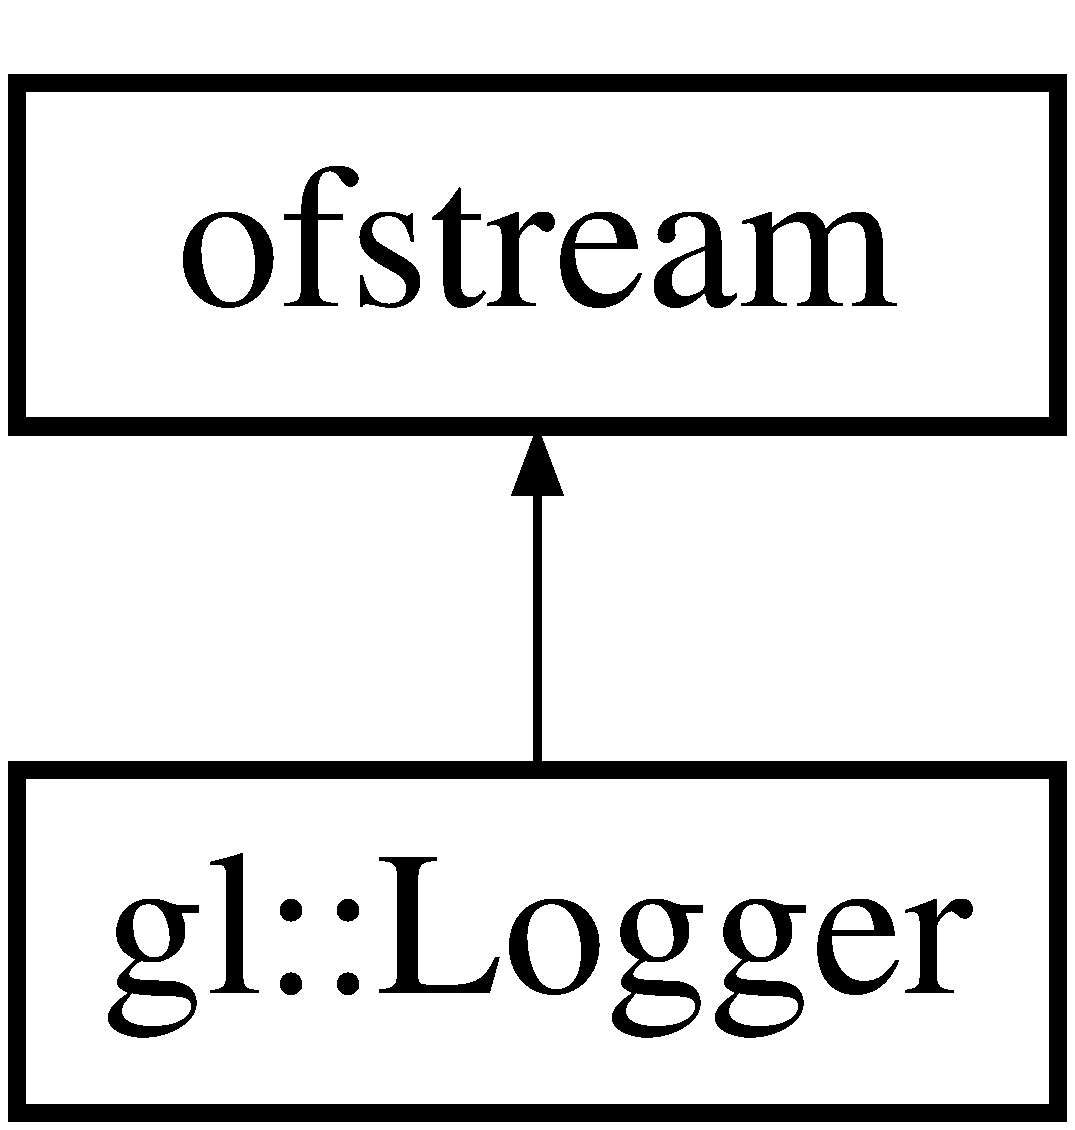
\includegraphics[height=2.000000cm]{classgl_1_1_logger}
\end{center}
\end{figure}
\subsection*{Public Member Functions}
\begin{DoxyCompactItemize}
\item 
\hyperlink{classgl_1_1_logger_ad36888d14605f37c4d4a6a528b63d03f}{Logger} (const std\-::string \&log\-File)
\item 
\hyperlink{classgl_1_1_logger_a067247e09fc5824c941536a7487acd3c}{$\sim$\-Logger} ()
\item 
\hyperlink{classgl_1_1_logger}{Logger} \& \hyperlink{classgl_1_1_logger_a1c7edf59e57196464b8e2844c33bddfa}{Log\-Time} ()
\end{DoxyCompactItemize}


\subsection{Detailed Description}


Definition at line 17 of file Logger.\-hpp.



\subsection{Constructor \& Destructor Documentation}
\hypertarget{classgl_1_1_logger_ad36888d14605f37c4d4a6a528b63d03f}{\index{gl\-::\-Logger@{gl\-::\-Logger}!Logger@{Logger}}
\index{Logger@{Logger}!gl::Logger@{gl\-::\-Logger}}
\subsubsection[{Logger}]{\setlength{\rightskip}{0pt plus 5cm}gl\-::\-Logger\-::\-Logger (
\begin{DoxyParamCaption}
\item[{const std\-::string \&}]{log\-File}
\end{DoxyParamCaption}
)}}\label{classgl_1_1_logger_ad36888d14605f37c4d4a6a528b63d03f}


Definition at line 17 of file Logger.\-cpp.

\hypertarget{classgl_1_1_logger_a067247e09fc5824c941536a7487acd3c}{\index{gl\-::\-Logger@{gl\-::\-Logger}!$\sim$\-Logger@{$\sim$\-Logger}}
\index{$\sim$\-Logger@{$\sim$\-Logger}!gl::Logger@{gl\-::\-Logger}}
\subsubsection[{$\sim$\-Logger}]{\setlength{\rightskip}{0pt plus 5cm}gl\-::\-Logger\-::$\sim$\-Logger (
\begin{DoxyParamCaption}
{}
\end{DoxyParamCaption}
)}}\label{classgl_1_1_logger_a067247e09fc5824c941536a7487acd3c}


Definition at line 27 of file Logger.\-cpp.



\subsection{Member Function Documentation}
\hypertarget{classgl_1_1_logger_a1c7edf59e57196464b8e2844c33bddfa}{\index{gl\-::\-Logger@{gl\-::\-Logger}!Log\-Time@{Log\-Time}}
\index{Log\-Time@{Log\-Time}!gl::Logger@{gl\-::\-Logger}}
\subsubsection[{Log\-Time}]{\setlength{\rightskip}{0pt plus 5cm}{\bf Logger} \& gl\-::\-Logger\-::\-Log\-Time (
\begin{DoxyParamCaption}
{}
\end{DoxyParamCaption}
)}}\label{classgl_1_1_logger_a1c7edf59e57196464b8e2844c33bddfa}


Definition at line 39 of file Logger.\-cpp.



The documentation for this class was generated from the following files\-:\begin{DoxyCompactItemize}
\item 
Glide/\hyperlink{_logger_8hpp}{Logger.\-hpp}\item 
Glide/\hyperlink{_logger_8cpp}{Logger.\-cpp}\end{DoxyCompactItemize}

\hypertarget{classtinyxml2_1_1_mem_pool}{\section{tinyxml2\-:\-:Mem\-Pool Class Reference}
\label{classtinyxml2_1_1_mem_pool}\index{tinyxml2\-::\-Mem\-Pool@{tinyxml2\-::\-Mem\-Pool}}
}


{\ttfamily \#include $<$tinyxml2.\-hpp$>$}

Inheritance diagram for tinyxml2\-:\-:Mem\-Pool\-:\begin{figure}[H]
\begin{center}
\leavevmode
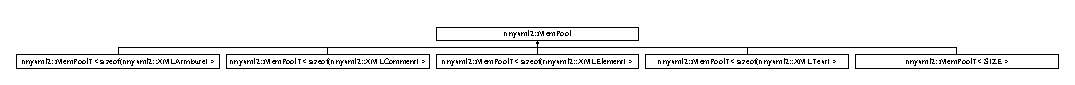
\includegraphics[height=0.691358cm]{classtinyxml2_1_1_mem_pool}
\end{center}
\end{figure}
\subsection*{Public Member Functions}
\begin{DoxyCompactItemize}
\item 
\hyperlink{classtinyxml2_1_1_mem_pool_a9101a0083d7370c85bd5aaaba7157f84}{Mem\-Pool} ()
\item 
virtual \hyperlink{classtinyxml2_1_1_mem_pool_ae55ad9e3faeca702e6ccbb38fdbcad72}{$\sim$\-Mem\-Pool} ()
\item 
virtual int \hyperlink{classtinyxml2_1_1_mem_pool_a0c518d49e3a94bde566f61e13b7240bb}{Item\-Size} () const =0
\item 
virtual void $\ast$ \hyperlink{classtinyxml2_1_1_mem_pool_a4f977b5fed752c0bbfe5295f469d6449}{Alloc} ()=0
\item 
virtual void \hyperlink{classtinyxml2_1_1_mem_pool_a49e3bfac2cba2ebd6776b31e571f64f7}{Free} (void $\ast$)=0
\item 
virtual void \hyperlink{classtinyxml2_1_1_mem_pool_ac5804dd1387b2e4de5eef710076a0db1}{Set\-Tracked} ()=0
\end{DoxyCompactItemize}


\subsection{Detailed Description}


Definition at line 295 of file tinyxml2.\-hpp.



\subsection{Constructor \& Destructor Documentation}
\hypertarget{classtinyxml2_1_1_mem_pool_a9101a0083d7370c85bd5aaaba7157f84}{\index{tinyxml2\-::\-Mem\-Pool@{tinyxml2\-::\-Mem\-Pool}!Mem\-Pool@{Mem\-Pool}}
\index{Mem\-Pool@{Mem\-Pool}!tinyxml2::MemPool@{tinyxml2\-::\-Mem\-Pool}}
\subsubsection[{Mem\-Pool}]{\setlength{\rightskip}{0pt plus 5cm}tinyxml2\-::\-Mem\-Pool\-::\-Mem\-Pool (
\begin{DoxyParamCaption}
{}
\end{DoxyParamCaption}
)\hspace{0.3cm}{\ttfamily [inline]}}}\label{classtinyxml2_1_1_mem_pool_a9101a0083d7370c85bd5aaaba7157f84}


Definition at line 298 of file tinyxml2.\-hpp.

\hypertarget{classtinyxml2_1_1_mem_pool_ae55ad9e3faeca702e6ccbb38fdbcad72}{\index{tinyxml2\-::\-Mem\-Pool@{tinyxml2\-::\-Mem\-Pool}!$\sim$\-Mem\-Pool@{$\sim$\-Mem\-Pool}}
\index{$\sim$\-Mem\-Pool@{$\sim$\-Mem\-Pool}!tinyxml2::MemPool@{tinyxml2\-::\-Mem\-Pool}}
\subsubsection[{$\sim$\-Mem\-Pool}]{\setlength{\rightskip}{0pt plus 5cm}virtual tinyxml2\-::\-Mem\-Pool\-::$\sim$\-Mem\-Pool (
\begin{DoxyParamCaption}
{}
\end{DoxyParamCaption}
)\hspace{0.3cm}{\ttfamily [inline]}, {\ttfamily [virtual]}}}\label{classtinyxml2_1_1_mem_pool_ae55ad9e3faeca702e6ccbb38fdbcad72}


Definition at line 299 of file tinyxml2.\-hpp.



\subsection{Member Function Documentation}
\hypertarget{classtinyxml2_1_1_mem_pool_a4f977b5fed752c0bbfe5295f469d6449}{\index{tinyxml2\-::\-Mem\-Pool@{tinyxml2\-::\-Mem\-Pool}!Alloc@{Alloc}}
\index{Alloc@{Alloc}!tinyxml2::MemPool@{tinyxml2\-::\-Mem\-Pool}}
\subsubsection[{Alloc}]{\setlength{\rightskip}{0pt plus 5cm}virtual void$\ast$ tinyxml2\-::\-Mem\-Pool\-::\-Alloc (
\begin{DoxyParamCaption}
{}
\end{DoxyParamCaption}
)\hspace{0.3cm}{\ttfamily [pure virtual]}}}\label{classtinyxml2_1_1_mem_pool_a4f977b5fed752c0bbfe5295f469d6449}


Implemented in \hyperlink{classtinyxml2_1_1_mem_pool_t_aa9d785a48ffe6ea1be679bab13464486}{tinyxml2\-::\-Mem\-Pool\-T$<$ S\-I\-Z\-E $>$}, \hyperlink{classtinyxml2_1_1_mem_pool_t_aa9d785a48ffe6ea1be679bab13464486}{tinyxml2\-::\-Mem\-Pool\-T$<$ sizeof(tinyxml2\-::\-X\-M\-L\-Comment) $>$}, \hyperlink{classtinyxml2_1_1_mem_pool_t_aa9d785a48ffe6ea1be679bab13464486}{tinyxml2\-::\-Mem\-Pool\-T$<$ sizeof(tinyxml2\-::\-X\-M\-L\-Text) $>$}, \hyperlink{classtinyxml2_1_1_mem_pool_t_aa9d785a48ffe6ea1be679bab13464486}{tinyxml2\-::\-Mem\-Pool\-T$<$ sizeof(tinyxml2\-::\-X\-M\-L\-Attribute) $>$}, and \hyperlink{classtinyxml2_1_1_mem_pool_t_aa9d785a48ffe6ea1be679bab13464486}{tinyxml2\-::\-Mem\-Pool\-T$<$ sizeof(tinyxml2\-::\-X\-M\-L\-Element) $>$}.

\hypertarget{classtinyxml2_1_1_mem_pool_a49e3bfac2cba2ebd6776b31e571f64f7}{\index{tinyxml2\-::\-Mem\-Pool@{tinyxml2\-::\-Mem\-Pool}!Free@{Free}}
\index{Free@{Free}!tinyxml2::MemPool@{tinyxml2\-::\-Mem\-Pool}}
\subsubsection[{Free}]{\setlength{\rightskip}{0pt plus 5cm}virtual void tinyxml2\-::\-Mem\-Pool\-::\-Free (
\begin{DoxyParamCaption}
\item[{void $\ast$}]{}
\end{DoxyParamCaption}
)\hspace{0.3cm}{\ttfamily [pure virtual]}}}\label{classtinyxml2_1_1_mem_pool_a49e3bfac2cba2ebd6776b31e571f64f7}


Implemented in \hyperlink{classtinyxml2_1_1_mem_pool_t_a4f1a0c434e9e3d7391e5c16ed4ee8c70}{tinyxml2\-::\-Mem\-Pool\-T$<$ S\-I\-Z\-E $>$}, \hyperlink{classtinyxml2_1_1_mem_pool_t_a4f1a0c434e9e3d7391e5c16ed4ee8c70}{tinyxml2\-::\-Mem\-Pool\-T$<$ sizeof(tinyxml2\-::\-X\-M\-L\-Comment) $>$}, \hyperlink{classtinyxml2_1_1_mem_pool_t_a4f1a0c434e9e3d7391e5c16ed4ee8c70}{tinyxml2\-::\-Mem\-Pool\-T$<$ sizeof(tinyxml2\-::\-X\-M\-L\-Text) $>$}, \hyperlink{classtinyxml2_1_1_mem_pool_t_a4f1a0c434e9e3d7391e5c16ed4ee8c70}{tinyxml2\-::\-Mem\-Pool\-T$<$ sizeof(tinyxml2\-::\-X\-M\-L\-Attribute) $>$}, and \hyperlink{classtinyxml2_1_1_mem_pool_t_a4f1a0c434e9e3d7391e5c16ed4ee8c70}{tinyxml2\-::\-Mem\-Pool\-T$<$ sizeof(tinyxml2\-::\-X\-M\-L\-Element) $>$}.

\hypertarget{classtinyxml2_1_1_mem_pool_a0c518d49e3a94bde566f61e13b7240bb}{\index{tinyxml2\-::\-Mem\-Pool@{tinyxml2\-::\-Mem\-Pool}!Item\-Size@{Item\-Size}}
\index{Item\-Size@{Item\-Size}!tinyxml2::MemPool@{tinyxml2\-::\-Mem\-Pool}}
\subsubsection[{Item\-Size}]{\setlength{\rightskip}{0pt plus 5cm}virtual int tinyxml2\-::\-Mem\-Pool\-::\-Item\-Size (
\begin{DoxyParamCaption}
{}
\end{DoxyParamCaption}
) const\hspace{0.3cm}{\ttfamily [pure virtual]}}}\label{classtinyxml2_1_1_mem_pool_a0c518d49e3a94bde566f61e13b7240bb}


Implemented in \hyperlink{classtinyxml2_1_1_mem_pool_t_a7ec8778fe99f6e332615a703be0b48bc}{tinyxml2\-::\-Mem\-Pool\-T$<$ S\-I\-Z\-E $>$}, \hyperlink{classtinyxml2_1_1_mem_pool_t_a7ec8778fe99f6e332615a703be0b48bc}{tinyxml2\-::\-Mem\-Pool\-T$<$ sizeof(tinyxml2\-::\-X\-M\-L\-Comment) $>$}, \hyperlink{classtinyxml2_1_1_mem_pool_t_a7ec8778fe99f6e332615a703be0b48bc}{tinyxml2\-::\-Mem\-Pool\-T$<$ sizeof(tinyxml2\-::\-X\-M\-L\-Text) $>$}, \hyperlink{classtinyxml2_1_1_mem_pool_t_a7ec8778fe99f6e332615a703be0b48bc}{tinyxml2\-::\-Mem\-Pool\-T$<$ sizeof(tinyxml2\-::\-X\-M\-L\-Attribute) $>$}, and \hyperlink{classtinyxml2_1_1_mem_pool_t_a7ec8778fe99f6e332615a703be0b48bc}{tinyxml2\-::\-Mem\-Pool\-T$<$ sizeof(tinyxml2\-::\-X\-M\-L\-Element) $>$}.

\hypertarget{classtinyxml2_1_1_mem_pool_ac5804dd1387b2e4de5eef710076a0db1}{\index{tinyxml2\-::\-Mem\-Pool@{tinyxml2\-::\-Mem\-Pool}!Set\-Tracked@{Set\-Tracked}}
\index{Set\-Tracked@{Set\-Tracked}!tinyxml2::MemPool@{tinyxml2\-::\-Mem\-Pool}}
\subsubsection[{Set\-Tracked}]{\setlength{\rightskip}{0pt plus 5cm}virtual void tinyxml2\-::\-Mem\-Pool\-::\-Set\-Tracked (
\begin{DoxyParamCaption}
{}
\end{DoxyParamCaption}
)\hspace{0.3cm}{\ttfamily [pure virtual]}}}\label{classtinyxml2_1_1_mem_pool_ac5804dd1387b2e4de5eef710076a0db1}


Implemented in \hyperlink{classtinyxml2_1_1_mem_pool_t_a7798932414916199a1bc0f9c3f368521}{tinyxml2\-::\-Mem\-Pool\-T$<$ S\-I\-Z\-E $>$}, \hyperlink{classtinyxml2_1_1_mem_pool_t_a7798932414916199a1bc0f9c3f368521}{tinyxml2\-::\-Mem\-Pool\-T$<$ sizeof(tinyxml2\-::\-X\-M\-L\-Comment) $>$}, \hyperlink{classtinyxml2_1_1_mem_pool_t_a7798932414916199a1bc0f9c3f368521}{tinyxml2\-::\-Mem\-Pool\-T$<$ sizeof(tinyxml2\-::\-X\-M\-L\-Text) $>$}, \hyperlink{classtinyxml2_1_1_mem_pool_t_a7798932414916199a1bc0f9c3f368521}{tinyxml2\-::\-Mem\-Pool\-T$<$ sizeof(tinyxml2\-::\-X\-M\-L\-Attribute) $>$}, and \hyperlink{classtinyxml2_1_1_mem_pool_t_a7798932414916199a1bc0f9c3f368521}{tinyxml2\-::\-Mem\-Pool\-T$<$ sizeof(tinyxml2\-::\-X\-M\-L\-Element) $>$}.



The documentation for this class was generated from the following file\-:\begin{DoxyCompactItemize}
\item 
Glide/\hyperlink{tinyxml2_8hpp}{tinyxml2.\-hpp}\end{DoxyCompactItemize}

\hypertarget{classtinyxml2_1_1_mem_pool_t}{\section{tinyxml2\-:\-:Mem\-Pool\-T$<$ S\-I\-Z\-E $>$ Class Template Reference}
\label{classtinyxml2_1_1_mem_pool_t}\index{tinyxml2\-::\-Mem\-Pool\-T$<$ S\-I\-Z\-E $>$@{tinyxml2\-::\-Mem\-Pool\-T$<$ S\-I\-Z\-E $>$}}
}


{\ttfamily \#include $<$tinyxml2.\-hpp$>$}

Inheritance diagram for tinyxml2\-:\-:Mem\-Pool\-T$<$ S\-I\-Z\-E $>$\-:\begin{figure}[H]
\begin{center}
\leavevmode
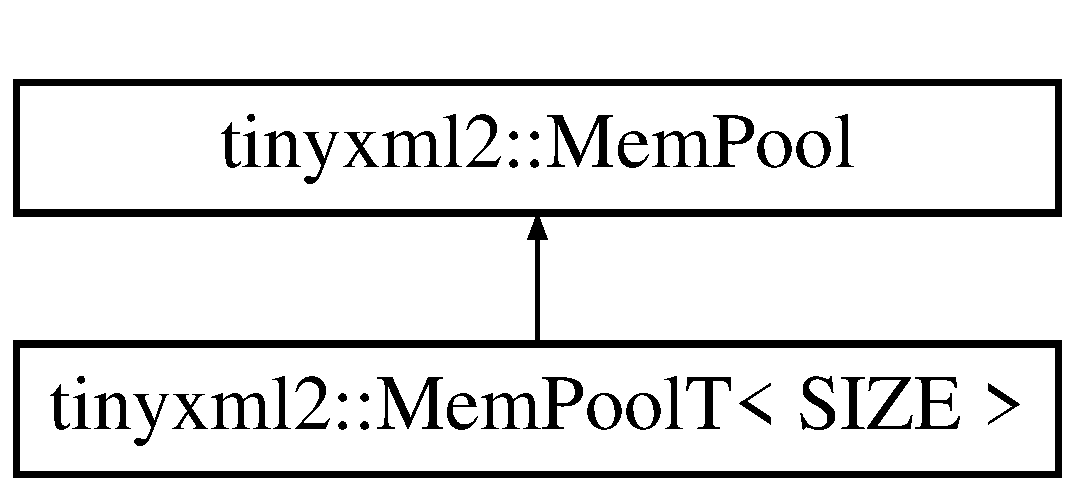
\includegraphics[height=2.000000cm]{classtinyxml2_1_1_mem_pool_t}
\end{center}
\end{figure}
\subsection*{Public Types}
\begin{DoxyCompactItemize}
\item 
enum \{ \hyperlink{classtinyxml2_1_1_mem_pool_t_a04cf45156e6f913f93972869ff8a1d94a4eeedbaa09fc9968120af6190e9e0988}{C\-O\-U\-N\-T} = (4$\ast$1024)/\-S\-I\-Z\-E
 \}
\end{DoxyCompactItemize}
\subsection*{Public Member Functions}
\begin{DoxyCompactItemize}
\item 
\hyperlink{classtinyxml2_1_1_mem_pool_t_a8a69a269ea72e292dde65309528ef64b}{Mem\-Pool\-T} ()
\item 
\hyperlink{classtinyxml2_1_1_mem_pool_t_ad6bb8346ad5b9a34f8f0051da5e3ed3f}{$\sim$\-Mem\-Pool\-T} ()
\item 
virtual int \hyperlink{classtinyxml2_1_1_mem_pool_t_a7ec8778fe99f6e332615a703be0b48bc}{Item\-Size} () const 
\item 
int \hyperlink{classtinyxml2_1_1_mem_pool_t_a56be11b7db6a7ef00db17088a7769aab}{Current\-Allocs} () const 
\item 
virtual void $\ast$ \hyperlink{classtinyxml2_1_1_mem_pool_t_aa9d785a48ffe6ea1be679bab13464486}{Alloc} ()
\item 
virtual void \hyperlink{classtinyxml2_1_1_mem_pool_t_a4f1a0c434e9e3d7391e5c16ed4ee8c70}{Free} (void $\ast$mem)
\item 
void \hyperlink{classtinyxml2_1_1_mem_pool_t_a0bc596f271e0f139822c534238b3f244}{Trace} (const char $\ast$name)
\item 
void \hyperlink{classtinyxml2_1_1_mem_pool_t_a7798932414916199a1bc0f9c3f368521}{Set\-Tracked} ()
\item 
int \hyperlink{classtinyxml2_1_1_mem_pool_t_a524b90d0edeac41964c06510757dce0f}{Untracked} () const 
\end{DoxyCompactItemize}


\subsection{Detailed Description}
\subsubsection*{template$<$int S\-I\-Z\-E$>$class tinyxml2\-::\-Mem\-Pool\-T$<$ S\-I\-Z\-E $>$}



Definition at line 312 of file tinyxml2.\-hpp.



\subsection{Member Enumeration Documentation}
\hypertarget{classtinyxml2_1_1_mem_pool_t_a04cf45156e6f913f93972869ff8a1d94}{\subsubsection[{anonymous enum}]{\setlength{\rightskip}{0pt plus 5cm}template$<$int S\-I\-Z\-E$>$ anonymous enum}}\label{classtinyxml2_1_1_mem_pool_t_a04cf45156e6f913f93972869ff8a1d94}
\begin{Desc}
\item[Enumerator]\par
\begin{description}
\index{C\-O\-U\-N\-T@{C\-O\-U\-N\-T}!tinyxml2\-::\-Mem\-Pool\-T@{tinyxml2\-::\-Mem\-Pool\-T}}\index{tinyxml2\-::\-Mem\-Pool\-T@{tinyxml2\-::\-Mem\-Pool\-T}!C\-O\-U\-N\-T@{C\-O\-U\-N\-T}}\item[{\em 
\hypertarget{classtinyxml2_1_1_mem_pool_t_a04cf45156e6f913f93972869ff8a1d94a4eeedbaa09fc9968120af6190e9e0988}{C\-O\-U\-N\-T}\label{classtinyxml2_1_1_mem_pool_t_a04cf45156e6f913f93972869ff8a1d94a4eeedbaa09fc9968120af6190e9e0988}
}]\end{description}
\end{Desc}


Definition at line 387 of file tinyxml2.\-hpp.



\subsection{Constructor \& Destructor Documentation}
\hypertarget{classtinyxml2_1_1_mem_pool_t_a8a69a269ea72e292dde65309528ef64b}{\index{tinyxml2\-::\-Mem\-Pool\-T@{tinyxml2\-::\-Mem\-Pool\-T}!Mem\-Pool\-T@{Mem\-Pool\-T}}
\index{Mem\-Pool\-T@{Mem\-Pool\-T}!tinyxml2::MemPoolT@{tinyxml2\-::\-Mem\-Pool\-T}}
\subsubsection[{Mem\-Pool\-T}]{\setlength{\rightskip}{0pt plus 5cm}template$<$int S\-I\-Z\-E$>$ {\bf tinyxml2\-::\-Mem\-Pool\-T}$<$ S\-I\-Z\-E $>$\-::{\bf Mem\-Pool\-T} (
\begin{DoxyParamCaption}
{}
\end{DoxyParamCaption}
)\hspace{0.3cm}{\ttfamily [inline]}}}\label{classtinyxml2_1_1_mem_pool_t_a8a69a269ea72e292dde65309528ef64b}


Definition at line 315 of file tinyxml2.\-hpp.

\hypertarget{classtinyxml2_1_1_mem_pool_t_ad6bb8346ad5b9a34f8f0051da5e3ed3f}{\index{tinyxml2\-::\-Mem\-Pool\-T@{tinyxml2\-::\-Mem\-Pool\-T}!$\sim$\-Mem\-Pool\-T@{$\sim$\-Mem\-Pool\-T}}
\index{$\sim$\-Mem\-Pool\-T@{$\sim$\-Mem\-Pool\-T}!tinyxml2::MemPoolT@{tinyxml2\-::\-Mem\-Pool\-T}}
\subsubsection[{$\sim$\-Mem\-Pool\-T}]{\setlength{\rightskip}{0pt plus 5cm}template$<$int S\-I\-Z\-E$>$ {\bf tinyxml2\-::\-Mem\-Pool\-T}$<$ S\-I\-Z\-E $>$\-::$\sim${\bf Mem\-Pool\-T} (
\begin{DoxyParamCaption}
{}
\end{DoxyParamCaption}
)\hspace{0.3cm}{\ttfamily [inline]}}}\label{classtinyxml2_1_1_mem_pool_t_ad6bb8346ad5b9a34f8f0051da5e3ed3f}


Definition at line 316 of file tinyxml2.\-hpp.



\subsection{Member Function Documentation}
\hypertarget{classtinyxml2_1_1_mem_pool_t_aa9d785a48ffe6ea1be679bab13464486}{\index{tinyxml2\-::\-Mem\-Pool\-T@{tinyxml2\-::\-Mem\-Pool\-T}!Alloc@{Alloc}}
\index{Alloc@{Alloc}!tinyxml2::MemPoolT@{tinyxml2\-::\-Mem\-Pool\-T}}
\subsubsection[{Alloc}]{\setlength{\rightskip}{0pt plus 5cm}template$<$int S\-I\-Z\-E$>$ virtual void$\ast$ {\bf tinyxml2\-::\-Mem\-Pool\-T}$<$ S\-I\-Z\-E $>$\-::Alloc (
\begin{DoxyParamCaption}
{}
\end{DoxyParamCaption}
)\hspace{0.3cm}{\ttfamily [inline]}, {\ttfamily [virtual]}}}\label{classtinyxml2_1_1_mem_pool_t_aa9d785a48ffe6ea1be679bab13464486}


Implements \hyperlink{classtinyxml2_1_1_mem_pool_a4f977b5fed752c0bbfe5295f469d6449}{tinyxml2\-::\-Mem\-Pool}.



Definition at line 330 of file tinyxml2.\-hpp.

\hypertarget{classtinyxml2_1_1_mem_pool_t_a56be11b7db6a7ef00db17088a7769aab}{\index{tinyxml2\-::\-Mem\-Pool\-T@{tinyxml2\-::\-Mem\-Pool\-T}!Current\-Allocs@{Current\-Allocs}}
\index{Current\-Allocs@{Current\-Allocs}!tinyxml2::MemPoolT@{tinyxml2\-::\-Mem\-Pool\-T}}
\subsubsection[{Current\-Allocs}]{\setlength{\rightskip}{0pt plus 5cm}template$<$int S\-I\-Z\-E$>$ int {\bf tinyxml2\-::\-Mem\-Pool\-T}$<$ S\-I\-Z\-E $>$\-::Current\-Allocs (
\begin{DoxyParamCaption}
{}
\end{DoxyParamCaption}
) const\hspace{0.3cm}{\ttfamily [inline]}}}\label{classtinyxml2_1_1_mem_pool_t_a56be11b7db6a7ef00db17088a7769aab}


Definition at line 326 of file tinyxml2.\-hpp.

\hypertarget{classtinyxml2_1_1_mem_pool_t_a4f1a0c434e9e3d7391e5c16ed4ee8c70}{\index{tinyxml2\-::\-Mem\-Pool\-T@{tinyxml2\-::\-Mem\-Pool\-T}!Free@{Free}}
\index{Free@{Free}!tinyxml2::MemPoolT@{tinyxml2\-::\-Mem\-Pool\-T}}
\subsubsection[{Free}]{\setlength{\rightskip}{0pt plus 5cm}template$<$int S\-I\-Z\-E$>$ virtual void {\bf tinyxml2\-::\-Mem\-Pool\-T}$<$ S\-I\-Z\-E $>$\-::Free (
\begin{DoxyParamCaption}
\item[{void $\ast$}]{mem}
\end{DoxyParamCaption}
)\hspace{0.3cm}{\ttfamily [inline]}, {\ttfamily [virtual]}}}\label{classtinyxml2_1_1_mem_pool_t_a4f1a0c434e9e3d7391e5c16ed4ee8c70}


Implements \hyperlink{classtinyxml2_1_1_mem_pool_a49e3bfac2cba2ebd6776b31e571f64f7}{tinyxml2\-::\-Mem\-Pool}.



Definition at line 353 of file tinyxml2.\-hpp.

\hypertarget{classtinyxml2_1_1_mem_pool_t_a7ec8778fe99f6e332615a703be0b48bc}{\index{tinyxml2\-::\-Mem\-Pool\-T@{tinyxml2\-::\-Mem\-Pool\-T}!Item\-Size@{Item\-Size}}
\index{Item\-Size@{Item\-Size}!tinyxml2::MemPoolT@{tinyxml2\-::\-Mem\-Pool\-T}}
\subsubsection[{Item\-Size}]{\setlength{\rightskip}{0pt plus 5cm}template$<$int S\-I\-Z\-E$>$ virtual int {\bf tinyxml2\-::\-Mem\-Pool\-T}$<$ S\-I\-Z\-E $>$\-::Item\-Size (
\begin{DoxyParamCaption}
{}
\end{DoxyParamCaption}
) const\hspace{0.3cm}{\ttfamily [inline]}, {\ttfamily [virtual]}}}\label{classtinyxml2_1_1_mem_pool_t_a7ec8778fe99f6e332615a703be0b48bc}


Implements \hyperlink{classtinyxml2_1_1_mem_pool_a0c518d49e3a94bde566f61e13b7240bb}{tinyxml2\-::\-Mem\-Pool}.



Definition at line 323 of file tinyxml2.\-hpp.

\hypertarget{classtinyxml2_1_1_mem_pool_t_a7798932414916199a1bc0f9c3f368521}{\index{tinyxml2\-::\-Mem\-Pool\-T@{tinyxml2\-::\-Mem\-Pool\-T}!Set\-Tracked@{Set\-Tracked}}
\index{Set\-Tracked@{Set\-Tracked}!tinyxml2::MemPoolT@{tinyxml2\-::\-Mem\-Pool\-T}}
\subsubsection[{Set\-Tracked}]{\setlength{\rightskip}{0pt plus 5cm}template$<$int S\-I\-Z\-E$>$ void {\bf tinyxml2\-::\-Mem\-Pool\-T}$<$ S\-I\-Z\-E $>$\-::Set\-Tracked (
\begin{DoxyParamCaption}
{}
\end{DoxyParamCaption}
)\hspace{0.3cm}{\ttfamily [inline]}, {\ttfamily [virtual]}}}\label{classtinyxml2_1_1_mem_pool_t_a7798932414916199a1bc0f9c3f368521}


Implements \hyperlink{classtinyxml2_1_1_mem_pool_ac5804dd1387b2e4de5eef710076a0db1}{tinyxml2\-::\-Mem\-Pool}.



Definition at line 370 of file tinyxml2.\-hpp.

\hypertarget{classtinyxml2_1_1_mem_pool_t_a0bc596f271e0f139822c534238b3f244}{\index{tinyxml2\-::\-Mem\-Pool\-T@{tinyxml2\-::\-Mem\-Pool\-T}!Trace@{Trace}}
\index{Trace@{Trace}!tinyxml2::MemPoolT@{tinyxml2\-::\-Mem\-Pool\-T}}
\subsubsection[{Trace}]{\setlength{\rightskip}{0pt plus 5cm}template$<$int S\-I\-Z\-E$>$ void {\bf tinyxml2\-::\-Mem\-Pool\-T}$<$ S\-I\-Z\-E $>$\-::Trace (
\begin{DoxyParamCaption}
\item[{const char $\ast$}]{name}
\end{DoxyParamCaption}
)\hspace{0.3cm}{\ttfamily [inline]}}}\label{classtinyxml2_1_1_mem_pool_t_a0bc596f271e0f139822c534238b3f244}


Definition at line 365 of file tinyxml2.\-hpp.

\hypertarget{classtinyxml2_1_1_mem_pool_t_a524b90d0edeac41964c06510757dce0f}{\index{tinyxml2\-::\-Mem\-Pool\-T@{tinyxml2\-::\-Mem\-Pool\-T}!Untracked@{Untracked}}
\index{Untracked@{Untracked}!tinyxml2::MemPoolT@{tinyxml2\-::\-Mem\-Pool\-T}}
\subsubsection[{Untracked}]{\setlength{\rightskip}{0pt plus 5cm}template$<$int S\-I\-Z\-E$>$ int {\bf tinyxml2\-::\-Mem\-Pool\-T}$<$ S\-I\-Z\-E $>$\-::Untracked (
\begin{DoxyParamCaption}
{}
\end{DoxyParamCaption}
) const\hspace{0.3cm}{\ttfamily [inline]}}}\label{classtinyxml2_1_1_mem_pool_t_a524b90d0edeac41964c06510757dce0f}


Definition at line 374 of file tinyxml2.\-hpp.



The documentation for this class was generated from the following file\-:\begin{DoxyCompactItemize}
\item 
Glide/\hyperlink{tinyxml2_8hpp}{tinyxml2.\-hpp}\end{DoxyCompactItemize}

\hypertarget{classgl_1_1_resource}{\section{gl\-:\-:Resource Class Reference}
\label{classgl_1_1_resource}\index{gl\-::\-Resource@{gl\-::\-Resource}}
}


{\ttfamily \#include $<$Resource.\-hpp$>$}

Inheritance diagram for gl\-:\-:Resource\-:\begin{figure}[H]
\begin{center}
\leavevmode
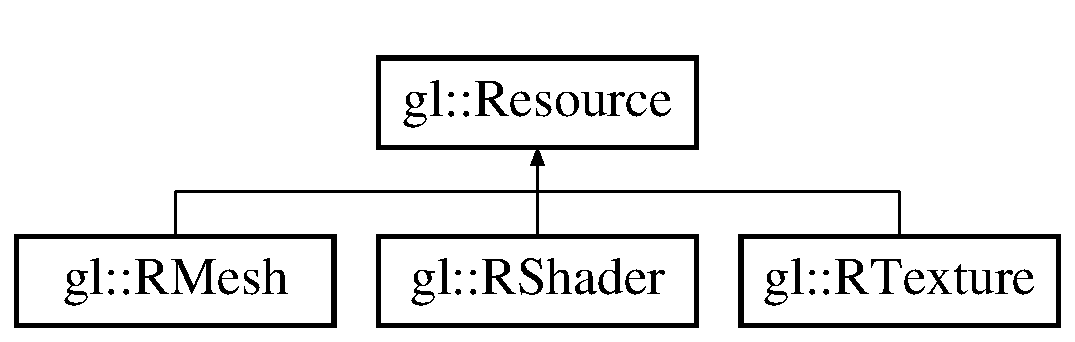
\includegraphics[height=2.000000cm]{classgl_1_1_resource}
\end{center}
\end{figure}
\subsection*{Classes}
\begin{DoxyCompactItemize}
\item 
class \hyperlink{classgl_1_1_resource_1_1_configuration}{Configuration}
\end{DoxyCompactItemize}
\subsection*{Public Types}
\begin{DoxyCompactItemize}
\item 
typedef \hyperlink{classgl_1_1_resource_1_1_configuration}{Resource\-::\-Configuration} \hyperlink{classgl_1_1_resource_a18683d13ef2edfbe9cb1e694497f6898}{Config\-Type}
\end{DoxyCompactItemize}
\subsection*{Public Member Functions}
\begin{DoxyCompactItemize}
\item 
\hyperlink{classgl_1_1_resource_a1edca9f900b5d2851661d81317ba0076}{Resource} (const \hyperlink{classgl_1_1_resource_1_1_configuration}{Resource\-::\-Configuration} \&config)
\item 
\hyperlink{classgl_1_1_resource_a15aa46dff1cf8f0f674f444831b8a288}{Resource} (\hyperlink{classgl_1_1_resource}{Resource} \&\&other)
\item 
\hyperlink{classgl_1_1_resource_aed04a0b3ef70ec4c834b87e29d50f761}{Resource} (const \hyperlink{classgl_1_1_resource}{Resource} \&other)=delete
\item 
\hyperlink{classgl_1_1_resource}{Resource} \& \hyperlink{classgl_1_1_resource_aa5d1a0dc03ebfeb6bdd2b12a795a9fdd}{operator=} (const \hyperlink{classgl_1_1_resource}{Resource} \&other)=delete
\item 
virtual \hyperlink{classgl_1_1_resource_aaabd5bae068524556573c4f9f026c130}{$\sim$\-Resource} ()
\item 
const std\-::string \& \hyperlink{classgl_1_1_resource_a303a83798d6fad7e933fa7745c9ec18d}{Get\-File} () const 
\end{DoxyCompactItemize}
\subsection*{Protected Attributes}
\begin{DoxyCompactItemize}
\item 
std\-::string \hyperlink{classgl_1_1_resource_a1e2c1b22896c2a996f79a3a0308b8ecc}{m\-File}
\end{DoxyCompactItemize}


\subsection{Detailed Description}
Base class for resources.

All resource classes take in either \hyperlink{classgl_1_1_resource_1_1_configuration}{Resource\-::\-Configuration} or a subclass of \hyperlink{classgl_1_1_resource_1_1_configuration}{Resource\-::\-Configuration} This is to provide a clean extentable api. Also the Resource\-Managers take in the proper Resource\-Sub\-Class\-::\-Config\-Type 

Definition at line 19 of file Resource.\-hpp.



\subsection{Member Typedef Documentation}
\hypertarget{classgl_1_1_resource_a18683d13ef2edfbe9cb1e694497f6898}{\index{gl\-::\-Resource@{gl\-::\-Resource}!Config\-Type@{Config\-Type}}
\index{Config\-Type@{Config\-Type}!gl::Resource@{gl\-::\-Resource}}
\subsubsection[{Config\-Type}]{\setlength{\rightskip}{0pt plus 5cm}typedef {\bf Resource\-::\-Configuration} {\bf gl\-::\-Resource\-::\-Config\-Type}}}\label{classgl_1_1_resource_a18683d13ef2edfbe9cb1e694497f6898}


Definition at line 22 of file Resource.\-hpp.



\subsection{Constructor \& Destructor Documentation}
\hypertarget{classgl_1_1_resource_a1edca9f900b5d2851661d81317ba0076}{\index{gl\-::\-Resource@{gl\-::\-Resource}!Resource@{Resource}}
\index{Resource@{Resource}!gl::Resource@{gl\-::\-Resource}}
\subsubsection[{Resource}]{\setlength{\rightskip}{0pt plus 5cm}gl\-::\-Resource\-::\-Resource (
\begin{DoxyParamCaption}
\item[{const {\bf Resource\-::\-Configuration} \&}]{config}
\end{DoxyParamCaption}
)}}\label{classgl_1_1_resource_a1edca9f900b5d2851661d81317ba0076}
\hyperlink{classgl_1_1_resource}{Resource}, base resource class. It's template argument is the comparer by which will be returned by Get\-I\-D() and also is the template type of the Resource\-Config base class. 

Definition at line 52 of file Resource.\-cpp.

\hypertarget{classgl_1_1_resource_a15aa46dff1cf8f0f674f444831b8a288}{\index{gl\-::\-Resource@{gl\-::\-Resource}!Resource@{Resource}}
\index{Resource@{Resource}!gl::Resource@{gl\-::\-Resource}}
\subsubsection[{Resource}]{\setlength{\rightskip}{0pt plus 5cm}gl\-::\-Resource\-::\-Resource (
\begin{DoxyParamCaption}
\item[{{\bf Resource} \&\&}]{other}
\end{DoxyParamCaption}
)}}\label{classgl_1_1_resource_a15aa46dff1cf8f0f674f444831b8a288}


Definition at line 45 of file Resource.\-cpp.

\hypertarget{classgl_1_1_resource_aed04a0b3ef70ec4c834b87e29d50f761}{\index{gl\-::\-Resource@{gl\-::\-Resource}!Resource@{Resource}}
\index{Resource@{Resource}!gl::Resource@{gl\-::\-Resource}}
\subsubsection[{Resource}]{\setlength{\rightskip}{0pt plus 5cm}gl\-::\-Resource\-::\-Resource (
\begin{DoxyParamCaption}
\item[{const {\bf Resource} \&}]{other}
\end{DoxyParamCaption}
)\hspace{0.3cm}{\ttfamily [delete]}}}\label{classgl_1_1_resource_aed04a0b3ef70ec4c834b87e29d50f761}
\hypertarget{classgl_1_1_resource_aaabd5bae068524556573c4f9f026c130}{\index{gl\-::\-Resource@{gl\-::\-Resource}!$\sim$\-Resource@{$\sim$\-Resource}}
\index{$\sim$\-Resource@{$\sim$\-Resource}!gl::Resource@{gl\-::\-Resource}}
\subsubsection[{$\sim$\-Resource}]{\setlength{\rightskip}{0pt plus 5cm}gl\-::\-Resource\-::$\sim$\-Resource (
\begin{DoxyParamCaption}
{}
\end{DoxyParamCaption}
)\hspace{0.3cm}{\ttfamily [virtual]}}}\label{classgl_1_1_resource_aaabd5bae068524556573c4f9f026c130}


Definition at line 59 of file Resource.\-cpp.



\subsection{Member Function Documentation}
\hypertarget{classgl_1_1_resource_a303a83798d6fad7e933fa7745c9ec18d}{\index{gl\-::\-Resource@{gl\-::\-Resource}!Get\-File@{Get\-File}}
\index{Get\-File@{Get\-File}!gl::Resource@{gl\-::\-Resource}}
\subsubsection[{Get\-File}]{\setlength{\rightskip}{0pt plus 5cm}const std\-::string \& gl\-::\-Resource\-::\-Get\-File (
\begin{DoxyParamCaption}
{}
\end{DoxyParamCaption}
) const}}\label{classgl_1_1_resource_a303a83798d6fad7e933fa7745c9ec18d}


Definition at line 64 of file Resource.\-cpp.

\hypertarget{classgl_1_1_resource_aa5d1a0dc03ebfeb6bdd2b12a795a9fdd}{\index{gl\-::\-Resource@{gl\-::\-Resource}!operator=@{operator=}}
\index{operator=@{operator=}!gl::Resource@{gl\-::\-Resource}}
\subsubsection[{operator=}]{\setlength{\rightskip}{0pt plus 5cm}{\bf Resource}\& gl\-::\-Resource\-::operator= (
\begin{DoxyParamCaption}
\item[{const {\bf Resource} \&}]{other}
\end{DoxyParamCaption}
)\hspace{0.3cm}{\ttfamily [delete]}}}\label{classgl_1_1_resource_aa5d1a0dc03ebfeb6bdd2b12a795a9fdd}


\subsection{Member Data Documentation}
\hypertarget{classgl_1_1_resource_a1e2c1b22896c2a996f79a3a0308b8ecc}{\index{gl\-::\-Resource@{gl\-::\-Resource}!m\-File@{m\-File}}
\index{m\-File@{m\-File}!gl::Resource@{gl\-::\-Resource}}
\subsubsection[{m\-File}]{\setlength{\rightskip}{0pt plus 5cm}std\-::string gl\-::\-Resource\-::m\-File\hspace{0.3cm}{\ttfamily [protected]}}}\label{classgl_1_1_resource_a1e2c1b22896c2a996f79a3a0308b8ecc}


Definition at line 38 of file Resource.\-hpp.



The documentation for this class was generated from the following files\-:\begin{DoxyCompactItemize}
\item 
Glide/\hyperlink{_resource_8hpp}{Resource.\-hpp}\item 
Glide/\hyperlink{_resource_8cpp}{Resource.\-cpp}\end{DoxyCompactItemize}

\hypertarget{classgl_1_1_resource_manager}{\section{gl\-:\-:Resource\-Manager$<$ Res\-Type, Key\-Type $>$ Class Template Reference}
\label{classgl_1_1_resource_manager}\index{gl\-::\-Resource\-Manager$<$ Res\-Type, Key\-Type $>$@{gl\-::\-Resource\-Manager$<$ Res\-Type, Key\-Type $>$}}
}


{\ttfamily \#include $<$Resource\-Manager.\-hpp$>$}

\subsection*{Public Member Functions}
\begin{DoxyCompactItemize}
\item 
\hyperlink{classgl_1_1_resource_manager_a8a03114e394305bea3cd67a611f3100c}{Resource\-Manager} ()
\item 
\hyperlink{classgl_1_1_resource_manager_a98923a7788170cdf6e3eb06f16c9c728}{$\sim$\-Resource\-Manager} ()
\item 
\hyperlink{_basic_types_8hpp_afdf0f22c576e6ee1b982f64b839c4bea}{Void} \hyperlink{classgl_1_1_resource_manager_acd4a15d51a31ff7871260bfe9d133b19}{Resource\-Add} (const typename Res\-Type\-::\-Config\-Type \&config, const Key\-Type \&key)
\item 
Res\-Type $\ast$ \hyperlink{classgl_1_1_resource_manager_a76295508c8e6d50a829898ee55a10b68}{Resource\-Get} (const Key\-Type \&key)
\item 
\hyperlink{_basic_types_8hpp_a11c112f01a7ad8f767fd48bc916463a3}{U\-Int} \hyperlink{classgl_1_1_resource_manager_ad0a49cad4c53ec3a44b348b7fa200729}{Size} () const 
\end{DoxyCompactItemize}
\subsection*{Protected Attributes}
\begin{DoxyCompactItemize}
\item 
std\-::map$<$ Key\-Type, \\*
std\-::unique\-\_\-ptr$<$ Res\-Type $>$ $>$ \hyperlink{classgl_1_1_resource_manager_a1e9a623c449cb5a99362f02058a60ae2}{m\-Resources}
\end{DoxyCompactItemize}


\subsection{Detailed Description}
\subsubsection*{template$<$class Res\-Type, class Key\-Type$>$class gl\-::\-Resource\-Manager$<$ Res\-Type, Key\-Type $>$}

template class for managing resources. Simple manages resources, by a template key type and the tempate resource type. You can use any type that can be compaired as a key. Resources are stored internally in a map. To create and load a resource call Resource\-Add with the configuration type of your resource and the key you wish to use for that resource. You can get the resource pointer by calling Resource\-Get with the key. 

Definition at line 24 of file Resource\-Manager.\-hpp.



\subsection{Constructor \& Destructor Documentation}
\hypertarget{classgl_1_1_resource_manager_a8a03114e394305bea3cd67a611f3100c}{\index{gl\-::\-Resource\-Manager@{gl\-::\-Resource\-Manager}!Resource\-Manager@{Resource\-Manager}}
\index{Resource\-Manager@{Resource\-Manager}!gl::ResourceManager@{gl\-::\-Resource\-Manager}}
\subsubsection[{Resource\-Manager}]{\setlength{\rightskip}{0pt plus 5cm}template$<$class Res\-Type , class Key\-Type $>$ {\bf gl\-::\-Resource\-Manager}$<$ Res\-Type, Key\-Type $>$\-::{\bf Resource\-Manager} (
\begin{DoxyParamCaption}
{}
\end{DoxyParamCaption}
)\hspace{0.3cm}{\ttfamily [inline]}}}\label{classgl_1_1_resource_manager_a8a03114e394305bea3cd67a611f3100c}


Definition at line 49 of file Resource\-Manager.\-hpp.

\hypertarget{classgl_1_1_resource_manager_a98923a7788170cdf6e3eb06f16c9c728}{\index{gl\-::\-Resource\-Manager@{gl\-::\-Resource\-Manager}!$\sim$\-Resource\-Manager@{$\sim$\-Resource\-Manager}}
\index{$\sim$\-Resource\-Manager@{$\sim$\-Resource\-Manager}!gl::ResourceManager@{gl\-::\-Resource\-Manager}}
\subsubsection[{$\sim$\-Resource\-Manager}]{\setlength{\rightskip}{0pt plus 5cm}template$<$class Res\-Type , class Key\-Type $>$ {\bf gl\-::\-Resource\-Manager}$<$ Res\-Type, Key\-Type $>$\-::$\sim${\bf Resource\-Manager} (
\begin{DoxyParamCaption}
{}
\end{DoxyParamCaption}
)\hspace{0.3cm}{\ttfamily [inline]}}}\label{classgl_1_1_resource_manager_a98923a7788170cdf6e3eb06f16c9c728}


Definition at line 55 of file Resource\-Manager.\-hpp.



\subsection{Member Function Documentation}
\hypertarget{classgl_1_1_resource_manager_acd4a15d51a31ff7871260bfe9d133b19}{\index{gl\-::\-Resource\-Manager@{gl\-::\-Resource\-Manager}!Resource\-Add@{Resource\-Add}}
\index{Resource\-Add@{Resource\-Add}!gl::ResourceManager@{gl\-::\-Resource\-Manager}}
\subsubsection[{Resource\-Add}]{\setlength{\rightskip}{0pt plus 5cm}template$<$class Res\-Type, class Key\-Type$>$ {\bf Void} {\bf gl\-::\-Resource\-Manager}$<$ Res\-Type, Key\-Type $>$\-::Resource\-Add (
\begin{DoxyParamCaption}
\item[{const typename Res\-Type\-::\-Config\-Type \&}]{config, }
\item[{const Key\-Type \&}]{key}
\end{DoxyParamCaption}
)\hspace{0.3cm}{\ttfamily [inline]}}}\label{classgl_1_1_resource_manager_acd4a15d51a31ff7871260bfe9d133b19}
Resource\-Add adds resource to the map. Will create the resource internally. The Key is the template paramter on Resource\-Config. The manager will grab the key from the config. 

Definition at line 61 of file Resource\-Manager.\-hpp.

\hypertarget{classgl_1_1_resource_manager_a76295508c8e6d50a829898ee55a10b68}{\index{gl\-::\-Resource\-Manager@{gl\-::\-Resource\-Manager}!Resource\-Get@{Resource\-Get}}
\index{Resource\-Get@{Resource\-Get}!gl::ResourceManager@{gl\-::\-Resource\-Manager}}
\subsubsection[{Resource\-Get}]{\setlength{\rightskip}{0pt plus 5cm}template$<$class Res\-Type , class Key\-Type$>$ Res\-Type $\ast$ {\bf gl\-::\-Resource\-Manager}$<$ Res\-Type, Key\-Type $>$\-::Resource\-Get (
\begin{DoxyParamCaption}
\item[{const Key\-Type \&}]{key}
\end{DoxyParamCaption}
)\hspace{0.3cm}{\ttfamily [inline]}}}\label{classgl_1_1_resource_manager_a76295508c8e6d50a829898ee55a10b68}
Resource\-Get returns a resource pointer by the map key, which is the Comparer template argument of the resource. 

Definition at line 72 of file Resource\-Manager.\-hpp.

\hypertarget{classgl_1_1_resource_manager_ad0a49cad4c53ec3a44b348b7fa200729}{\index{gl\-::\-Resource\-Manager@{gl\-::\-Resource\-Manager}!Size@{Size}}
\index{Size@{Size}!gl::ResourceManager@{gl\-::\-Resource\-Manager}}
\subsubsection[{Size}]{\setlength{\rightskip}{0pt plus 5cm}template$<$class Res\-Type , class Key\-Type $>$ {\bf U\-Int} {\bf gl\-::\-Resource\-Manager}$<$ Res\-Type, Key\-Type $>$\-::Size (
\begin{DoxyParamCaption}
{}
\end{DoxyParamCaption}
) const\hspace{0.3cm}{\ttfamily [inline]}}}\label{classgl_1_1_resource_manager_ad0a49cad4c53ec3a44b348b7fa200729}


Definition at line 85 of file Resource\-Manager.\-hpp.



\subsection{Member Data Documentation}
\hypertarget{classgl_1_1_resource_manager_a1e9a623c449cb5a99362f02058a60ae2}{\index{gl\-::\-Resource\-Manager@{gl\-::\-Resource\-Manager}!m\-Resources@{m\-Resources}}
\index{m\-Resources@{m\-Resources}!gl::ResourceManager@{gl\-::\-Resource\-Manager}}
\subsubsection[{m\-Resources}]{\setlength{\rightskip}{0pt plus 5cm}template$<$class Res\-Type, class Key\-Type$>$ std\-::map$<$ Key\-Type, std\-::unique\-\_\-ptr$<$ Res\-Type $>$ $>$ {\bf gl\-::\-Resource\-Manager}$<$ Res\-Type, Key\-Type $>$\-::m\-Resources\hspace{0.3cm}{\ttfamily [protected]}}}\label{classgl_1_1_resource_manager_a1e9a623c449cb5a99362f02058a60ae2}


Definition at line 45 of file Resource\-Manager.\-hpp.



The documentation for this class was generated from the following file\-:\begin{DoxyCompactItemize}
\item 
Glide/\hyperlink{_resource_manager_8hpp}{Resource\-Manager.\-hpp}\end{DoxyCompactItemize}

\hypertarget{classgl_1_1_r_mesh}{\section{gl\-:\-:R\-Mesh Class Reference}
\label{classgl_1_1_r_mesh}\index{gl\-::\-R\-Mesh@{gl\-::\-R\-Mesh}}
}


{\ttfamily \#include $<$R\-Mesh.\-hpp$>$}

Inheritance diagram for gl\-:\-:R\-Mesh\-:\begin{figure}[H]
\begin{center}
\leavevmode
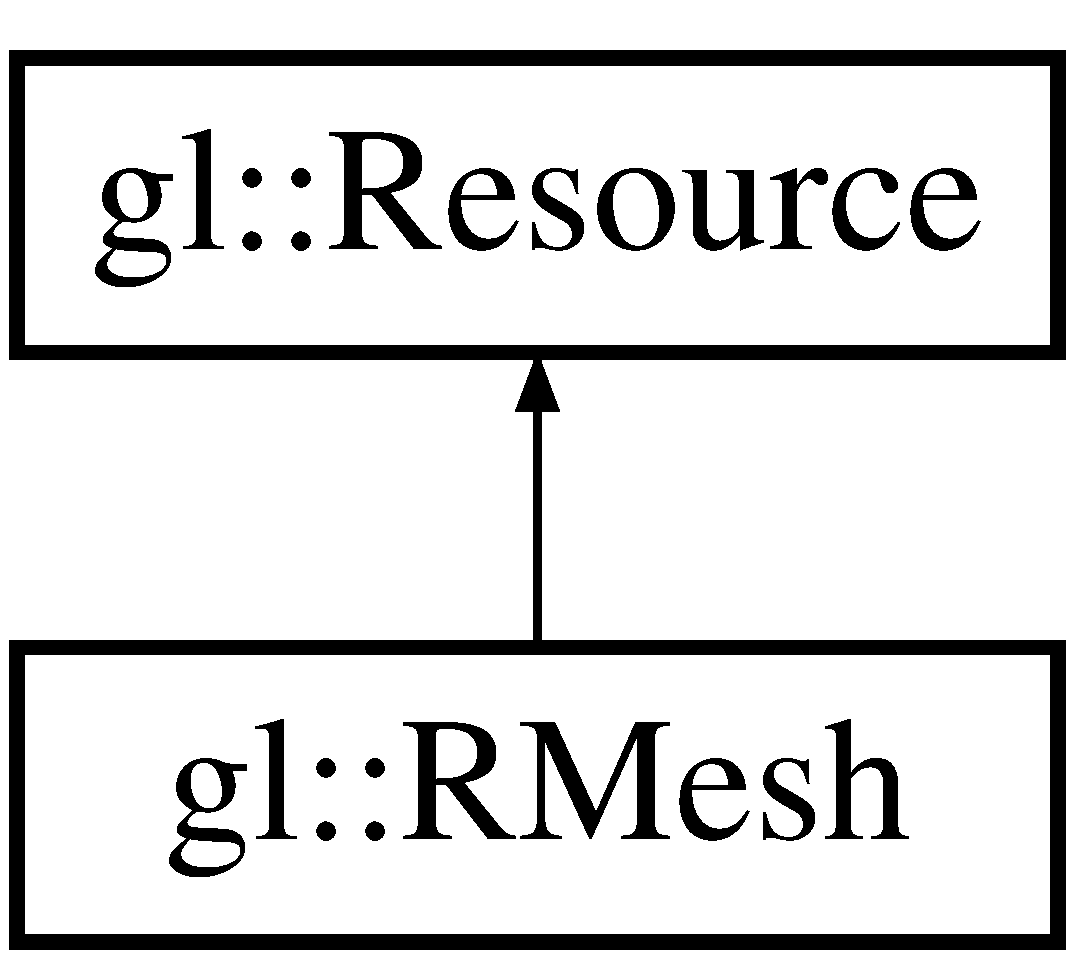
\includegraphics[height=2.000000cm]{classgl_1_1_r_mesh}
\end{center}
\end{figure}
\subsection*{Classes}
\begin{DoxyCompactItemize}
\item 
class \hyperlink{classgl_1_1_r_mesh_1_1_configuration}{Configuration}
\end{DoxyCompactItemize}
\subsection*{Public Types}
\begin{DoxyCompactItemize}
\item 
typedef \hyperlink{classgl_1_1_r_mesh_1_1_configuration}{R\-Mesh\-::\-Configuration} \hyperlink{classgl_1_1_r_mesh_a79f410d038549426f50fb60ea46f3ebd}{Config\-Type}
\end{DoxyCompactItemize}
\subsection*{Public Member Functions}
\begin{DoxyCompactItemize}
\item 
\hyperlink{classgl_1_1_r_mesh_a4d0f4e90717bf32767364d3e2bb7d0fa}{R\-Mesh} (const \hyperlink{classgl_1_1_r_mesh_1_1_configuration}{R\-Mesh\-::\-Configuration} \&config)
\item 
virtual \hyperlink{classgl_1_1_r_mesh_afb0492fdc604d1db50a17d84fb46250e}{$\sim$\-R\-Mesh} ()
\item 
\hyperlink{_basic_types_8hpp_afdf0f22c576e6ee1b982f64b839c4bea}{Void} \hyperlink{classgl_1_1_r_mesh_afe64f717298a3d2d3eaa6271156dc54a}{Bind} () const 
\item 
\hyperlink{classgl_1_1_r_texture}{R\-Texture} $\ast$ \hyperlink{classgl_1_1_r_mesh_ada1eb2ce86eda9fa108347604b9f4068}{Get\-Texture} () const 
\item 
G\-Luint \hyperlink{classgl_1_1_r_mesh_aad7602f1be7e89104e2a37e3067794ff}{Get\-Vertex\-Index\-Count} () const 
\end{DoxyCompactItemize}
\subsection*{Static Public Member Functions}
\begin{DoxyCompactItemize}
\item 
static \hyperlink{_basic_types_8hpp_afdf0f22c576e6ee1b982f64b839c4bea}{Void} \hyperlink{classgl_1_1_r_mesh_ac8e930f887c2b59eff37b7722115bd4f}{Bind\-Null} ()
\end{DoxyCompactItemize}
\subsection*{Protected Attributes}
\begin{DoxyCompactItemize}
\item 
\hyperlink{classgl_1_1_r_texture}{R\-Texture} $\ast$ \hyperlink{classgl_1_1_r_mesh_a409110e20a5f2d2a39229f6f71445b53}{mp\-Texture}
\item 
\hyperlink{_basic_types_8hpp_a11c112f01a7ad8f767fd48bc916463a3}{U\-Int} \hyperlink{classgl_1_1_r_mesh_a4edcf25786adf2e264c61c6b8d7f401f}{m\-Vertex\-Count}
\item 
G\-Luint \hyperlink{classgl_1_1_r_mesh_afdfd8a88b91096eb4b23ca9786587c61}{m\-Vertex\-Index\-Count}
\item 
G\-Luint \hyperlink{classgl_1_1_r_mesh_a9667468e4f7e16f934a155bd28954e7d}{m\-Vao}
\item 
G\-Luint \hyperlink{classgl_1_1_r_mesh_a89115eb9f8ee1ebd8dc55e68f886170a}{m\-Vbo\-Positions}
\item 
G\-Luint \hyperlink{classgl_1_1_r_mesh_a5efc2fecfc6da14de8008b1e04694fb8}{m\-Vbo\-Normals}
\item 
G\-Luint \hyperlink{classgl_1_1_r_mesh_aff4a64a5d46ccd3e1ca67cad783765d7}{m\-Vbo\-U\-Vs}
\item 
G\-Luint \hyperlink{classgl_1_1_r_mesh_a1f5091fc89b32918e1a4cc92ec41a852}{m\-Vbo\-Indicies}
\end{DoxyCompactItemize}


\subsection{Detailed Description}
\hyperlink{classgl_1_1_r_mesh}{R\-Mesh} class represents a mesh. Since we are using Assimp to load entire scenes this object just takes in the open\-G\-L vao and vbos created by the scene loader, and stores those ids for rendering and destruction later. 

Definition at line 18 of file R\-Mesh.\-hpp.



\subsection{Member Typedef Documentation}
\hypertarget{classgl_1_1_r_mesh_a79f410d038549426f50fb60ea46f3ebd}{\index{gl\-::\-R\-Mesh@{gl\-::\-R\-Mesh}!Config\-Type@{Config\-Type}}
\index{Config\-Type@{Config\-Type}!gl::RMesh@{gl\-::\-R\-Mesh}}
\subsubsection[{Config\-Type}]{\setlength{\rightskip}{0pt plus 5cm}typedef {\bf R\-Mesh\-::\-Configuration} {\bf gl\-::\-R\-Mesh\-::\-Config\-Type}}}\label{classgl_1_1_r_mesh_a79f410d038549426f50fb60ea46f3ebd}


Definition at line 21 of file R\-Mesh.\-hpp.



\subsection{Constructor \& Destructor Documentation}
\hypertarget{classgl_1_1_r_mesh_a4d0f4e90717bf32767364d3e2bb7d0fa}{\index{gl\-::\-R\-Mesh@{gl\-::\-R\-Mesh}!R\-Mesh@{R\-Mesh}}
\index{R\-Mesh@{R\-Mesh}!gl::RMesh@{gl\-::\-R\-Mesh}}
\subsubsection[{R\-Mesh}]{\setlength{\rightskip}{0pt plus 5cm}gl\-::\-R\-Mesh\-::\-R\-Mesh (
\begin{DoxyParamCaption}
\item[{const {\bf R\-Mesh\-::\-Configuration} \&}]{config}
\end{DoxyParamCaption}
)}}\label{classgl_1_1_r_mesh_a4d0f4e90717bf32767364d3e2bb7d0fa}


Definition at line 10 of file R\-Mesh.\-cpp.

\hypertarget{classgl_1_1_r_mesh_afb0492fdc604d1db50a17d84fb46250e}{\index{gl\-::\-R\-Mesh@{gl\-::\-R\-Mesh}!$\sim$\-R\-Mesh@{$\sim$\-R\-Mesh}}
\index{$\sim$\-R\-Mesh@{$\sim$\-R\-Mesh}!gl::RMesh@{gl\-::\-R\-Mesh}}
\subsubsection[{$\sim$\-R\-Mesh}]{\setlength{\rightskip}{0pt plus 5cm}gl\-::\-R\-Mesh\-::$\sim$\-R\-Mesh (
\begin{DoxyParamCaption}
{}
\end{DoxyParamCaption}
)\hspace{0.3cm}{\ttfamily [virtual]}}}\label{classgl_1_1_r_mesh_afb0492fdc604d1db50a17d84fb46250e}


Definition at line 26 of file R\-Mesh.\-cpp.



\subsection{Member Function Documentation}
\hypertarget{classgl_1_1_r_mesh_afe64f717298a3d2d3eaa6271156dc54a}{\index{gl\-::\-R\-Mesh@{gl\-::\-R\-Mesh}!Bind@{Bind}}
\index{Bind@{Bind}!gl::RMesh@{gl\-::\-R\-Mesh}}
\subsubsection[{Bind}]{\setlength{\rightskip}{0pt plus 5cm}{\bf Void} gl\-::\-R\-Mesh\-::\-Bind (
\begin{DoxyParamCaption}
{}
\end{DoxyParamCaption}
) const}}\label{classgl_1_1_r_mesh_afe64f717298a3d2d3eaa6271156dc54a}
Bind this mesh to open\-G\-L's rendering system. 

Definition at line 61 of file R\-Mesh.\-cpp.

\hypertarget{classgl_1_1_r_mesh_ac8e930f887c2b59eff37b7722115bd4f}{\index{gl\-::\-R\-Mesh@{gl\-::\-R\-Mesh}!Bind\-Null@{Bind\-Null}}
\index{Bind\-Null@{Bind\-Null}!gl::RMesh@{gl\-::\-R\-Mesh}}
\subsubsection[{Bind\-Null}]{\setlength{\rightskip}{0pt plus 5cm}{\bf Void} gl\-::\-R\-Mesh\-::\-Bind\-Null (
\begin{DoxyParamCaption}
{}
\end{DoxyParamCaption}
)\hspace{0.3cm}{\ttfamily [static]}}}\label{classgl_1_1_r_mesh_ac8e930f887c2b59eff37b7722115bd4f}
Binds null to open\-G\-L's rendering system. 

Definition at line 66 of file R\-Mesh.\-cpp.

\hypertarget{classgl_1_1_r_mesh_ada1eb2ce86eda9fa108347604b9f4068}{\index{gl\-::\-R\-Mesh@{gl\-::\-R\-Mesh}!Get\-Texture@{Get\-Texture}}
\index{Get\-Texture@{Get\-Texture}!gl::RMesh@{gl\-::\-R\-Mesh}}
\subsubsection[{Get\-Texture}]{\setlength{\rightskip}{0pt plus 5cm}{\bf R\-Texture} $\ast$ gl\-::\-R\-Mesh\-::\-Get\-Texture (
\begin{DoxyParamCaption}
{}
\end{DoxyParamCaption}
) const}}\label{classgl_1_1_r_mesh_ada1eb2ce86eda9fa108347604b9f4068}
returns the texture associated with this mesh. 

Definition at line 71 of file R\-Mesh.\-cpp.

\hypertarget{classgl_1_1_r_mesh_aad7602f1be7e89104e2a37e3067794ff}{\index{gl\-::\-R\-Mesh@{gl\-::\-R\-Mesh}!Get\-Vertex\-Index\-Count@{Get\-Vertex\-Index\-Count}}
\index{Get\-Vertex\-Index\-Count@{Get\-Vertex\-Index\-Count}!gl::RMesh@{gl\-::\-R\-Mesh}}
\subsubsection[{Get\-Vertex\-Index\-Count}]{\setlength{\rightskip}{0pt plus 5cm}G\-Luint gl\-::\-R\-Mesh\-::\-Get\-Vertex\-Index\-Count (
\begin{DoxyParamCaption}
{}
\end{DoxyParamCaption}
) const}}\label{classgl_1_1_r_mesh_aad7602f1be7e89104e2a37e3067794ff}
retuns the vertex index count. You need this when rendering meshes with index buffers. 

Definition at line 76 of file R\-Mesh.\-cpp.



\subsection{Member Data Documentation}
\hypertarget{classgl_1_1_r_mesh_a409110e20a5f2d2a39229f6f71445b53}{\index{gl\-::\-R\-Mesh@{gl\-::\-R\-Mesh}!mp\-Texture@{mp\-Texture}}
\index{mp\-Texture@{mp\-Texture}!gl::RMesh@{gl\-::\-R\-Mesh}}
\subsubsection[{mp\-Texture}]{\setlength{\rightskip}{0pt plus 5cm}{\bf R\-Texture}$\ast$ gl\-::\-R\-Mesh\-::mp\-Texture\hspace{0.3cm}{\ttfamily [protected]}}}\label{classgl_1_1_r_mesh_a409110e20a5f2d2a39229f6f71445b53}


Definition at line 49 of file R\-Mesh.\-hpp.

\hypertarget{classgl_1_1_r_mesh_a9667468e4f7e16f934a155bd28954e7d}{\index{gl\-::\-R\-Mesh@{gl\-::\-R\-Mesh}!m\-Vao@{m\-Vao}}
\index{m\-Vao@{m\-Vao}!gl::RMesh@{gl\-::\-R\-Mesh}}
\subsubsection[{m\-Vao}]{\setlength{\rightskip}{0pt plus 5cm}G\-Luint gl\-::\-R\-Mesh\-::m\-Vao\hspace{0.3cm}{\ttfamily [protected]}}}\label{classgl_1_1_r_mesh_a9667468e4f7e16f934a155bd28954e7d}


Definition at line 52 of file R\-Mesh.\-hpp.

\hypertarget{classgl_1_1_r_mesh_a1f5091fc89b32918e1a4cc92ec41a852}{\index{gl\-::\-R\-Mesh@{gl\-::\-R\-Mesh}!m\-Vbo\-Indicies@{m\-Vbo\-Indicies}}
\index{m\-Vbo\-Indicies@{m\-Vbo\-Indicies}!gl::RMesh@{gl\-::\-R\-Mesh}}
\subsubsection[{m\-Vbo\-Indicies}]{\setlength{\rightskip}{0pt plus 5cm}G\-Luint gl\-::\-R\-Mesh\-::m\-Vbo\-Indicies\hspace{0.3cm}{\ttfamily [protected]}}}\label{classgl_1_1_r_mesh_a1f5091fc89b32918e1a4cc92ec41a852}


Definition at line 56 of file R\-Mesh.\-hpp.

\hypertarget{classgl_1_1_r_mesh_a5efc2fecfc6da14de8008b1e04694fb8}{\index{gl\-::\-R\-Mesh@{gl\-::\-R\-Mesh}!m\-Vbo\-Normals@{m\-Vbo\-Normals}}
\index{m\-Vbo\-Normals@{m\-Vbo\-Normals}!gl::RMesh@{gl\-::\-R\-Mesh}}
\subsubsection[{m\-Vbo\-Normals}]{\setlength{\rightskip}{0pt plus 5cm}G\-Luint gl\-::\-R\-Mesh\-::m\-Vbo\-Normals\hspace{0.3cm}{\ttfamily [protected]}}}\label{classgl_1_1_r_mesh_a5efc2fecfc6da14de8008b1e04694fb8}


Definition at line 54 of file R\-Mesh.\-hpp.

\hypertarget{classgl_1_1_r_mesh_a89115eb9f8ee1ebd8dc55e68f886170a}{\index{gl\-::\-R\-Mesh@{gl\-::\-R\-Mesh}!m\-Vbo\-Positions@{m\-Vbo\-Positions}}
\index{m\-Vbo\-Positions@{m\-Vbo\-Positions}!gl::RMesh@{gl\-::\-R\-Mesh}}
\subsubsection[{m\-Vbo\-Positions}]{\setlength{\rightskip}{0pt plus 5cm}G\-Luint gl\-::\-R\-Mesh\-::m\-Vbo\-Positions\hspace{0.3cm}{\ttfamily [protected]}}}\label{classgl_1_1_r_mesh_a89115eb9f8ee1ebd8dc55e68f886170a}


Definition at line 53 of file R\-Mesh.\-hpp.

\hypertarget{classgl_1_1_r_mesh_aff4a64a5d46ccd3e1ca67cad783765d7}{\index{gl\-::\-R\-Mesh@{gl\-::\-R\-Mesh}!m\-Vbo\-U\-Vs@{m\-Vbo\-U\-Vs}}
\index{m\-Vbo\-U\-Vs@{m\-Vbo\-U\-Vs}!gl::RMesh@{gl\-::\-R\-Mesh}}
\subsubsection[{m\-Vbo\-U\-Vs}]{\setlength{\rightskip}{0pt plus 5cm}G\-Luint gl\-::\-R\-Mesh\-::m\-Vbo\-U\-Vs\hspace{0.3cm}{\ttfamily [protected]}}}\label{classgl_1_1_r_mesh_aff4a64a5d46ccd3e1ca67cad783765d7}


Definition at line 55 of file R\-Mesh.\-hpp.

\hypertarget{classgl_1_1_r_mesh_a4edcf25786adf2e264c61c6b8d7f401f}{\index{gl\-::\-R\-Mesh@{gl\-::\-R\-Mesh}!m\-Vertex\-Count@{m\-Vertex\-Count}}
\index{m\-Vertex\-Count@{m\-Vertex\-Count}!gl::RMesh@{gl\-::\-R\-Mesh}}
\subsubsection[{m\-Vertex\-Count}]{\setlength{\rightskip}{0pt plus 5cm}{\bf U\-Int} gl\-::\-R\-Mesh\-::m\-Vertex\-Count\hspace{0.3cm}{\ttfamily [protected]}}}\label{classgl_1_1_r_mesh_a4edcf25786adf2e264c61c6b8d7f401f}


Definition at line 50 of file R\-Mesh.\-hpp.

\hypertarget{classgl_1_1_r_mesh_afdfd8a88b91096eb4b23ca9786587c61}{\index{gl\-::\-R\-Mesh@{gl\-::\-R\-Mesh}!m\-Vertex\-Index\-Count@{m\-Vertex\-Index\-Count}}
\index{m\-Vertex\-Index\-Count@{m\-Vertex\-Index\-Count}!gl::RMesh@{gl\-::\-R\-Mesh}}
\subsubsection[{m\-Vertex\-Index\-Count}]{\setlength{\rightskip}{0pt plus 5cm}G\-Luint gl\-::\-R\-Mesh\-::m\-Vertex\-Index\-Count\hspace{0.3cm}{\ttfamily [protected]}}}\label{classgl_1_1_r_mesh_afdfd8a88b91096eb4b23ca9786587c61}


Definition at line 51 of file R\-Mesh.\-hpp.



The documentation for this class was generated from the following files\-:\begin{DoxyCompactItemize}
\item 
Glide/\hyperlink{_r_mesh_8hpp}{R\-Mesh.\-hpp}\item 
Glide/\hyperlink{_r_mesh_8cpp}{R\-Mesh.\-cpp}\end{DoxyCompactItemize}

\hypertarget{classgl_1_1_r_shader}{\section{gl\-:\-:R\-Shader Class Reference}
\label{classgl_1_1_r_shader}\index{gl\-::\-R\-Shader@{gl\-::\-R\-Shader}}
}


{\ttfamily \#include $<$R\-Shader.\-hpp$>$}

Inheritance diagram for gl\-:\-:R\-Shader\-:\begin{figure}[H]
\begin{center}
\leavevmode
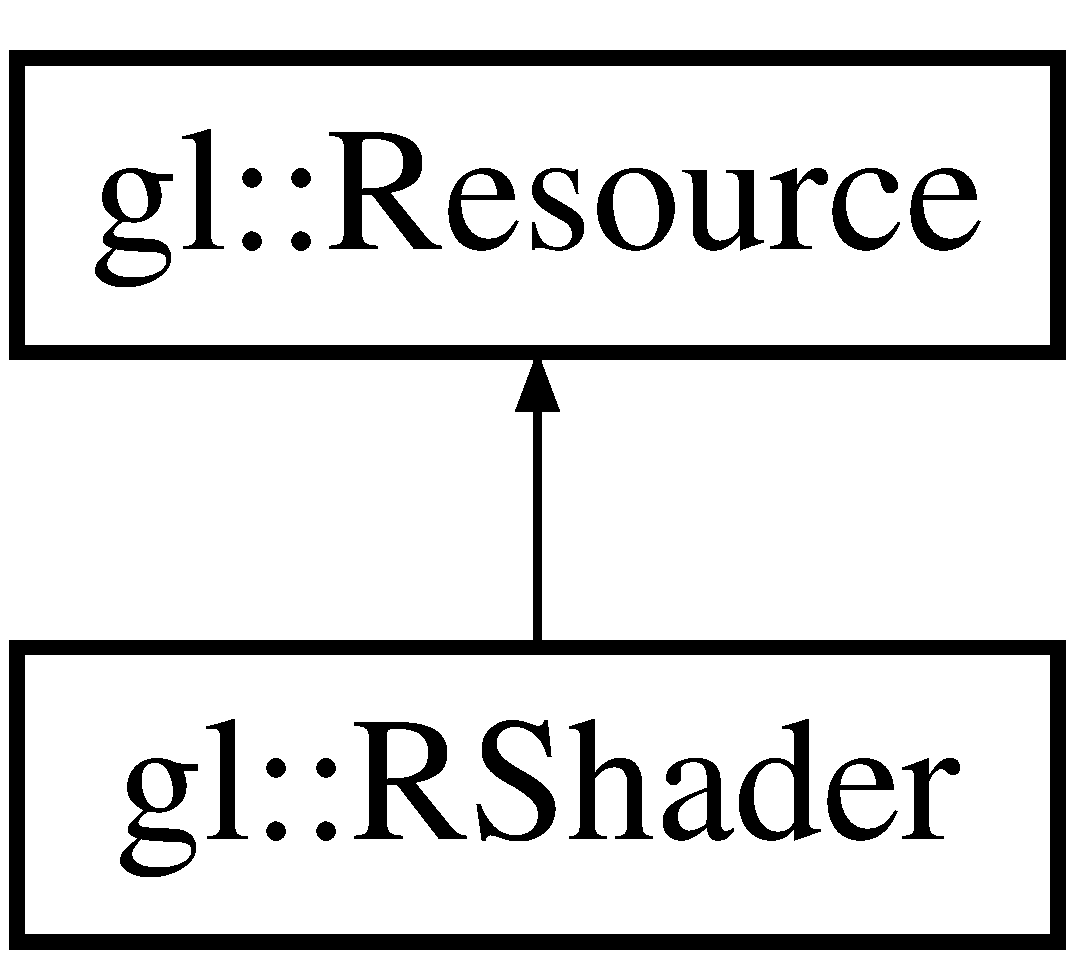
\includegraphics[height=2.000000cm]{classgl_1_1_r_shader}
\end{center}
\end{figure}
\subsection*{Classes}
\begin{DoxyCompactItemize}
\item 
class \hyperlink{classgl_1_1_r_shader_1_1_configuration}{Configuration}
\end{DoxyCompactItemize}
\subsection*{Public Types}
\begin{DoxyCompactItemize}
\item 
typedef \hyperlink{classgl_1_1_r_shader_1_1_configuration}{R\-Shader\-::\-Configuration} \hyperlink{classgl_1_1_r_shader_a737d7ce7dc0057760c6ff971aebdb3ff}{Config\-Type}
\end{DoxyCompactItemize}
\subsection*{Public Member Functions}
\begin{DoxyCompactItemize}
\item 
\hyperlink{classgl_1_1_r_shader_a8ed3d356636aa22d0d88679aa1ae1318}{R\-Shader} (const \hyperlink{classgl_1_1_r_shader_1_1_configuration}{R\-Shader\-::\-Configuration} \&config)
\item 
virtual \hyperlink{classgl_1_1_r_shader_ad3263f03a21e05a6f21f748aea8bbea5}{$\sim$\-R\-Shader} ()
\item 
std\-::string \hyperlink{classgl_1_1_r_shader_a058ce8e2bdbe39a1b76d677b188cd26a}{Get\-Vertex\-File} () const 
\item 
std\-::string \hyperlink{classgl_1_1_r_shader_add834ab6c12435ce12e857b31f2fd8b4}{Get\-Frag\-File} () const 
\item 
\hyperlink{_basic_types_8hpp_afdf0f22c576e6ee1b982f64b839c4bea}{Void} \hyperlink{classgl_1_1_r_shader_a339447b0d43a51a40774c9ac66717d20}{Set\-Uniform} (const char $\ast$p\-Uniform\-Name, const glm\-::mat4 \&mat)
\item 
\hyperlink{_basic_types_8hpp_afdf0f22c576e6ee1b982f64b839c4bea}{Void} \hyperlink{classgl_1_1_r_shader_ac8bc1b4975b08ece9a2b9ffc43d8e5f1}{Set\-Uniform} (const char $\ast$p\-Uniform\-Name, const glm\-::vec3 \&vec3)
\item 
\hyperlink{_basic_types_8hpp_afdf0f22c576e6ee1b982f64b839c4bea}{Void} \hyperlink{classgl_1_1_r_shader_a6abdc89ac6a89c0a78faa43018e3d1ad}{Set\-Uniform} (const char $\ast$p\-Uniform\-Name, const G\-Lfloat f)
\item 
\hyperlink{_basic_types_8hpp_afdf0f22c576e6ee1b982f64b839c4bea}{Void} \hyperlink{classgl_1_1_r_shader_a908a3cbe2bb85bff5e50eff0d0d9670f}{Set\-Uniform} (const char $\ast$p\-Uniform\-Name, const G\-Lint i)
\item 
\hyperlink{_basic_types_8hpp_afdf0f22c576e6ee1b982f64b839c4bea}{Void} \hyperlink{classgl_1_1_r_shader_ab45639a1ede87dfc0f4a8458dd5d00e8}{Set\-Uniform} (const char $\ast$p\-Uniform\-Name, const G\-Lboolean b)
\item 
\hyperlink{_basic_types_8hpp_afdf0f22c576e6ee1b982f64b839c4bea}{Void} \hyperlink{classgl_1_1_r_shader_a1a003461d4856a855a3a07f26daf1cb3}{Bind} () const 
\end{DoxyCompactItemize}
\subsection*{Static Public Member Functions}
\begin{DoxyCompactItemize}
\item 
static \hyperlink{_basic_types_8hpp_afdf0f22c576e6ee1b982f64b839c4bea}{Void} \hyperlink{classgl_1_1_r_shader_a61530fe10eb2f39469a706ca42f07336}{Bind\-Null} ()
\end{DoxyCompactItemize}
\subsection*{Protected Member Functions}
\begin{DoxyCompactItemize}
\item 
\hyperlink{_basic_types_8hpp_afdf0f22c576e6ee1b982f64b839c4bea}{Void} \hyperlink{classgl_1_1_r_shader_a2935e72e2bb4b93b61af39c998000b4c}{Load\-Shaders} ()
\end{DoxyCompactItemize}
\subsection*{Protected Attributes}
\begin{DoxyCompactItemize}
\item 
std\-::string \hyperlink{classgl_1_1_r_shader_a2285ac811c39bd59866a0239e04932b2}{m\-Vertex\-File}
\item 
std\-::string \hyperlink{classgl_1_1_r_shader_a6ce293498749d93a4fbc991b17a4cf70}{m\-Frag\-File}
\item 
G\-Luint \hyperlink{classgl_1_1_r_shader_a61ad380e879e29f8c052cad73158c54e}{m\-Program\-I\-D}
\item 
G\-Luint \hyperlink{classgl_1_1_r_shader_ab0996603afd00f5ce3a6b20479103083}{m\-Vert\-I\-D}
\item 
G\-Luint \hyperlink{classgl_1_1_r_shader_a0e077d5a150093c7af3c9ce047fcbe8d}{m\-Frag\-I\-D}
\end{DoxyCompactItemize}


\subsection{Detailed Description}
\hyperlink{classgl_1_1_r_shader}{R\-Shader} class represents a shader program. A shader program is made of two files at least. There must be a vertex shader and a fragment shader.

T\-O\-D\-O\-: write a function that loads vertex and fragment independantly. This way you can write a virtual Load\-Shader and have it load other shader like geometry and tesselation. 

Definition at line 22 of file R\-Shader.\-hpp.



\subsection{Member Typedef Documentation}
\hypertarget{classgl_1_1_r_shader_a737d7ce7dc0057760c6ff971aebdb3ff}{\index{gl\-::\-R\-Shader@{gl\-::\-R\-Shader}!Config\-Type@{Config\-Type}}
\index{Config\-Type@{Config\-Type}!gl::RShader@{gl\-::\-R\-Shader}}
\subsubsection[{Config\-Type}]{\setlength{\rightskip}{0pt plus 5cm}typedef {\bf R\-Shader\-::\-Configuration} {\bf gl\-::\-R\-Shader\-::\-Config\-Type}}}\label{classgl_1_1_r_shader_a737d7ce7dc0057760c6ff971aebdb3ff}


Definition at line 25 of file R\-Shader.\-hpp.



\subsection{Constructor \& Destructor Documentation}
\hypertarget{classgl_1_1_r_shader_a8ed3d356636aa22d0d88679aa1ae1318}{\index{gl\-::\-R\-Shader@{gl\-::\-R\-Shader}!R\-Shader@{R\-Shader}}
\index{R\-Shader@{R\-Shader}!gl::RShader@{gl\-::\-R\-Shader}}
\subsubsection[{R\-Shader}]{\setlength{\rightskip}{0pt plus 5cm}gl\-::\-R\-Shader\-::\-R\-Shader (
\begin{DoxyParamCaption}
\item[{const {\bf R\-Shader\-::\-Configuration} \&}]{config}
\end{DoxyParamCaption}
)}}\label{classgl_1_1_r_shader_a8ed3d356636aa22d0d88679aa1ae1318}


Definition at line 10 of file R\-Shader.\-cpp.

\hypertarget{classgl_1_1_r_shader_ad3263f03a21e05a6f21f748aea8bbea5}{\index{gl\-::\-R\-Shader@{gl\-::\-R\-Shader}!$\sim$\-R\-Shader@{$\sim$\-R\-Shader}}
\index{$\sim$\-R\-Shader@{$\sim$\-R\-Shader}!gl::RShader@{gl\-::\-R\-Shader}}
\subsubsection[{$\sim$\-R\-Shader}]{\setlength{\rightskip}{0pt plus 5cm}gl\-::\-R\-Shader\-::$\sim$\-R\-Shader (
\begin{DoxyParamCaption}
{}
\end{DoxyParamCaption}
)\hspace{0.3cm}{\ttfamily [virtual]}}}\label{classgl_1_1_r_shader_ad3263f03a21e05a6f21f748aea8bbea5}


Definition at line 22 of file R\-Shader.\-cpp.



\subsection{Member Function Documentation}
\hypertarget{classgl_1_1_r_shader_a1a003461d4856a855a3a07f26daf1cb3}{\index{gl\-::\-R\-Shader@{gl\-::\-R\-Shader}!Bind@{Bind}}
\index{Bind@{Bind}!gl::RShader@{gl\-::\-R\-Shader}}
\subsubsection[{Bind}]{\setlength{\rightskip}{0pt plus 5cm}{\bf Void} gl\-::\-R\-Shader\-::\-Bind (
\begin{DoxyParamCaption}
{}
\end{DoxyParamCaption}
) const}}\label{classgl_1_1_r_shader_a1a003461d4856a855a3a07f26daf1cb3}
Binds this shader program to open\-G\-L rendering system. 

Definition at line 208 of file R\-Shader.\-cpp.

\hypertarget{classgl_1_1_r_shader_a61530fe10eb2f39469a706ca42f07336}{\index{gl\-::\-R\-Shader@{gl\-::\-R\-Shader}!Bind\-Null@{Bind\-Null}}
\index{Bind\-Null@{Bind\-Null}!gl::RShader@{gl\-::\-R\-Shader}}
\subsubsection[{Bind\-Null}]{\setlength{\rightskip}{0pt plus 5cm}{\bf Void} gl\-::\-R\-Shader\-::\-Bind\-Null (
\begin{DoxyParamCaption}
{}
\end{DoxyParamCaption}
)\hspace{0.3cm}{\ttfamily [static]}}}\label{classgl_1_1_r_shader_a61530fe10eb2f39469a706ca42f07336}
Binds null program to open\-G\-L rendering system. 

Definition at line 213 of file R\-Shader.\-cpp.

\hypertarget{classgl_1_1_r_shader_add834ab6c12435ce12e857b31f2fd8b4}{\index{gl\-::\-R\-Shader@{gl\-::\-R\-Shader}!Get\-Frag\-File@{Get\-Frag\-File}}
\index{Get\-Frag\-File@{Get\-Frag\-File}!gl::RShader@{gl\-::\-R\-Shader}}
\subsubsection[{Get\-Frag\-File}]{\setlength{\rightskip}{0pt plus 5cm}std\-::string gl\-::\-R\-Shader\-::\-Get\-Frag\-File (
\begin{DoxyParamCaption}
{}
\end{DoxyParamCaption}
) const}}\label{classgl_1_1_r_shader_add834ab6c12435ce12e857b31f2fd8b4}
\hypertarget{classgl_1_1_r_shader_a058ce8e2bdbe39a1b76d677b188cd26a}{\index{gl\-::\-R\-Shader@{gl\-::\-R\-Shader}!Get\-Vertex\-File@{Get\-Vertex\-File}}
\index{Get\-Vertex\-File@{Get\-Vertex\-File}!gl::RShader@{gl\-::\-R\-Shader}}
\subsubsection[{Get\-Vertex\-File}]{\setlength{\rightskip}{0pt plus 5cm}std\-::string gl\-::\-R\-Shader\-::\-Get\-Vertex\-File (
\begin{DoxyParamCaption}
{}
\end{DoxyParamCaption}
) const}}\label{classgl_1_1_r_shader_a058ce8e2bdbe39a1b76d677b188cd26a}
\hypertarget{classgl_1_1_r_shader_a2935e72e2bb4b93b61af39c998000b4c}{\index{gl\-::\-R\-Shader@{gl\-::\-R\-Shader}!Load\-Shaders@{Load\-Shaders}}
\index{Load\-Shaders@{Load\-Shaders}!gl::RShader@{gl\-::\-R\-Shader}}
\subsubsection[{Load\-Shaders}]{\setlength{\rightskip}{0pt plus 5cm}{\bf Void} gl\-::\-R\-Shader\-::\-Load\-Shaders (
\begin{DoxyParamCaption}
{}
\end{DoxyParamCaption}
)\hspace{0.3cm}{\ttfamily [protected]}}}\label{classgl_1_1_r_shader_a2935e72e2bb4b93b61af39c998000b4c}


Definition at line 28 of file R\-Shader.\-cpp.

\hypertarget{classgl_1_1_r_shader_a339447b0d43a51a40774c9ac66717d20}{\index{gl\-::\-R\-Shader@{gl\-::\-R\-Shader}!Set\-Uniform@{Set\-Uniform}}
\index{Set\-Uniform@{Set\-Uniform}!gl::RShader@{gl\-::\-R\-Shader}}
\subsubsection[{Set\-Uniform}]{\setlength{\rightskip}{0pt plus 5cm}{\bf Void} gl\-::\-R\-Shader\-::\-Set\-Uniform (
\begin{DoxyParamCaption}
\item[{const char $\ast$}]{p\-Uniform\-Name, }
\item[{const glm\-::mat4 \&}]{mat}
\end{DoxyParamCaption}
)}}\label{classgl_1_1_r_shader_a339447b0d43a51a40774c9ac66717d20}


Definition at line 197 of file R\-Shader.\-cpp.

\hypertarget{classgl_1_1_r_shader_ac8bc1b4975b08ece9a2b9ffc43d8e5f1}{\index{gl\-::\-R\-Shader@{gl\-::\-R\-Shader}!Set\-Uniform@{Set\-Uniform}}
\index{Set\-Uniform@{Set\-Uniform}!gl::RShader@{gl\-::\-R\-Shader}}
\subsubsection[{Set\-Uniform}]{\setlength{\rightskip}{0pt plus 5cm}{\bf Void} gl\-::\-R\-Shader\-::\-Set\-Uniform (
\begin{DoxyParamCaption}
\item[{const char $\ast$}]{p\-Uniform\-Name, }
\item[{const glm\-::vec3 \&}]{vec3}
\end{DoxyParamCaption}
)}}\label{classgl_1_1_r_shader_ac8bc1b4975b08ece9a2b9ffc43d8e5f1}
\hypertarget{classgl_1_1_r_shader_a6abdc89ac6a89c0a78faa43018e3d1ad}{\index{gl\-::\-R\-Shader@{gl\-::\-R\-Shader}!Set\-Uniform@{Set\-Uniform}}
\index{Set\-Uniform@{Set\-Uniform}!gl::RShader@{gl\-::\-R\-Shader}}
\subsubsection[{Set\-Uniform}]{\setlength{\rightskip}{0pt plus 5cm}{\bf Void} gl\-::\-R\-Shader\-::\-Set\-Uniform (
\begin{DoxyParamCaption}
\item[{const char $\ast$}]{p\-Uniform\-Name, }
\item[{const G\-Lfloat}]{f}
\end{DoxyParamCaption}
)}}\label{classgl_1_1_r_shader_a6abdc89ac6a89c0a78faa43018e3d1ad}
\hypertarget{classgl_1_1_r_shader_a908a3cbe2bb85bff5e50eff0d0d9670f}{\index{gl\-::\-R\-Shader@{gl\-::\-R\-Shader}!Set\-Uniform@{Set\-Uniform}}
\index{Set\-Uniform@{Set\-Uniform}!gl::RShader@{gl\-::\-R\-Shader}}
\subsubsection[{Set\-Uniform}]{\setlength{\rightskip}{0pt plus 5cm}{\bf Void} gl\-::\-R\-Shader\-::\-Set\-Uniform (
\begin{DoxyParamCaption}
\item[{const char $\ast$}]{p\-Uniform\-Name, }
\item[{const G\-Lint}]{i}
\end{DoxyParamCaption}
)}}\label{classgl_1_1_r_shader_a908a3cbe2bb85bff5e50eff0d0d9670f}
\hypertarget{classgl_1_1_r_shader_ab45639a1ede87dfc0f4a8458dd5d00e8}{\index{gl\-::\-R\-Shader@{gl\-::\-R\-Shader}!Set\-Uniform@{Set\-Uniform}}
\index{Set\-Uniform@{Set\-Uniform}!gl::RShader@{gl\-::\-R\-Shader}}
\subsubsection[{Set\-Uniform}]{\setlength{\rightskip}{0pt plus 5cm}{\bf Void} gl\-::\-R\-Shader\-::\-Set\-Uniform (
\begin{DoxyParamCaption}
\item[{const char $\ast$}]{p\-Uniform\-Name, }
\item[{const G\-Lboolean}]{b}
\end{DoxyParamCaption}
)}}\label{classgl_1_1_r_shader_ab45639a1ede87dfc0f4a8458dd5d00e8}


\subsection{Member Data Documentation}
\hypertarget{classgl_1_1_r_shader_a6ce293498749d93a4fbc991b17a4cf70}{\index{gl\-::\-R\-Shader@{gl\-::\-R\-Shader}!m\-Frag\-File@{m\-Frag\-File}}
\index{m\-Frag\-File@{m\-Frag\-File}!gl::RShader@{gl\-::\-R\-Shader}}
\subsubsection[{m\-Frag\-File}]{\setlength{\rightskip}{0pt plus 5cm}std\-::string gl\-::\-R\-Shader\-::m\-Frag\-File\hspace{0.3cm}{\ttfamily [protected]}}}\label{classgl_1_1_r_shader_a6ce293498749d93a4fbc991b17a4cf70}


Definition at line 53 of file R\-Shader.\-hpp.

\hypertarget{classgl_1_1_r_shader_a0e077d5a150093c7af3c9ce047fcbe8d}{\index{gl\-::\-R\-Shader@{gl\-::\-R\-Shader}!m\-Frag\-I\-D@{m\-Frag\-I\-D}}
\index{m\-Frag\-I\-D@{m\-Frag\-I\-D}!gl::RShader@{gl\-::\-R\-Shader}}
\subsubsection[{m\-Frag\-I\-D}]{\setlength{\rightskip}{0pt plus 5cm}G\-Luint gl\-::\-R\-Shader\-::m\-Frag\-I\-D\hspace{0.3cm}{\ttfamily [protected]}}}\label{classgl_1_1_r_shader_a0e077d5a150093c7af3c9ce047fcbe8d}


Definition at line 57 of file R\-Shader.\-hpp.

\hypertarget{classgl_1_1_r_shader_a61ad380e879e29f8c052cad73158c54e}{\index{gl\-::\-R\-Shader@{gl\-::\-R\-Shader}!m\-Program\-I\-D@{m\-Program\-I\-D}}
\index{m\-Program\-I\-D@{m\-Program\-I\-D}!gl::RShader@{gl\-::\-R\-Shader}}
\subsubsection[{m\-Program\-I\-D}]{\setlength{\rightskip}{0pt plus 5cm}G\-Luint gl\-::\-R\-Shader\-::m\-Program\-I\-D\hspace{0.3cm}{\ttfamily [protected]}}}\label{classgl_1_1_r_shader_a61ad380e879e29f8c052cad73158c54e}


Definition at line 55 of file R\-Shader.\-hpp.

\hypertarget{classgl_1_1_r_shader_a2285ac811c39bd59866a0239e04932b2}{\index{gl\-::\-R\-Shader@{gl\-::\-R\-Shader}!m\-Vertex\-File@{m\-Vertex\-File}}
\index{m\-Vertex\-File@{m\-Vertex\-File}!gl::RShader@{gl\-::\-R\-Shader}}
\subsubsection[{m\-Vertex\-File}]{\setlength{\rightskip}{0pt plus 5cm}std\-::string gl\-::\-R\-Shader\-::m\-Vertex\-File\hspace{0.3cm}{\ttfamily [protected]}}}\label{classgl_1_1_r_shader_a2285ac811c39bd59866a0239e04932b2}


Definition at line 52 of file R\-Shader.\-hpp.

\hypertarget{classgl_1_1_r_shader_ab0996603afd00f5ce3a6b20479103083}{\index{gl\-::\-R\-Shader@{gl\-::\-R\-Shader}!m\-Vert\-I\-D@{m\-Vert\-I\-D}}
\index{m\-Vert\-I\-D@{m\-Vert\-I\-D}!gl::RShader@{gl\-::\-R\-Shader}}
\subsubsection[{m\-Vert\-I\-D}]{\setlength{\rightskip}{0pt plus 5cm}G\-Luint gl\-::\-R\-Shader\-::m\-Vert\-I\-D\hspace{0.3cm}{\ttfamily [protected]}}}\label{classgl_1_1_r_shader_ab0996603afd00f5ce3a6b20479103083}


Definition at line 56 of file R\-Shader.\-hpp.



The documentation for this class was generated from the following files\-:\begin{DoxyCompactItemize}
\item 
Glide/\hyperlink{_r_shader_8hpp}{R\-Shader.\-hpp}\item 
Glide/\hyperlink{_r_shader_8cpp}{R\-Shader.\-cpp}\end{DoxyCompactItemize}

\hypertarget{classgl_1_1_r_texture}{\section{gl\-:\-:R\-Texture Class Reference}
\label{classgl_1_1_r_texture}\index{gl\-::\-R\-Texture@{gl\-::\-R\-Texture}}
}


{\ttfamily \#include $<$R\-Texture.\-hpp$>$}

Inheritance diagram for gl\-:\-:R\-Texture\-:\begin{figure}[H]
\begin{center}
\leavevmode
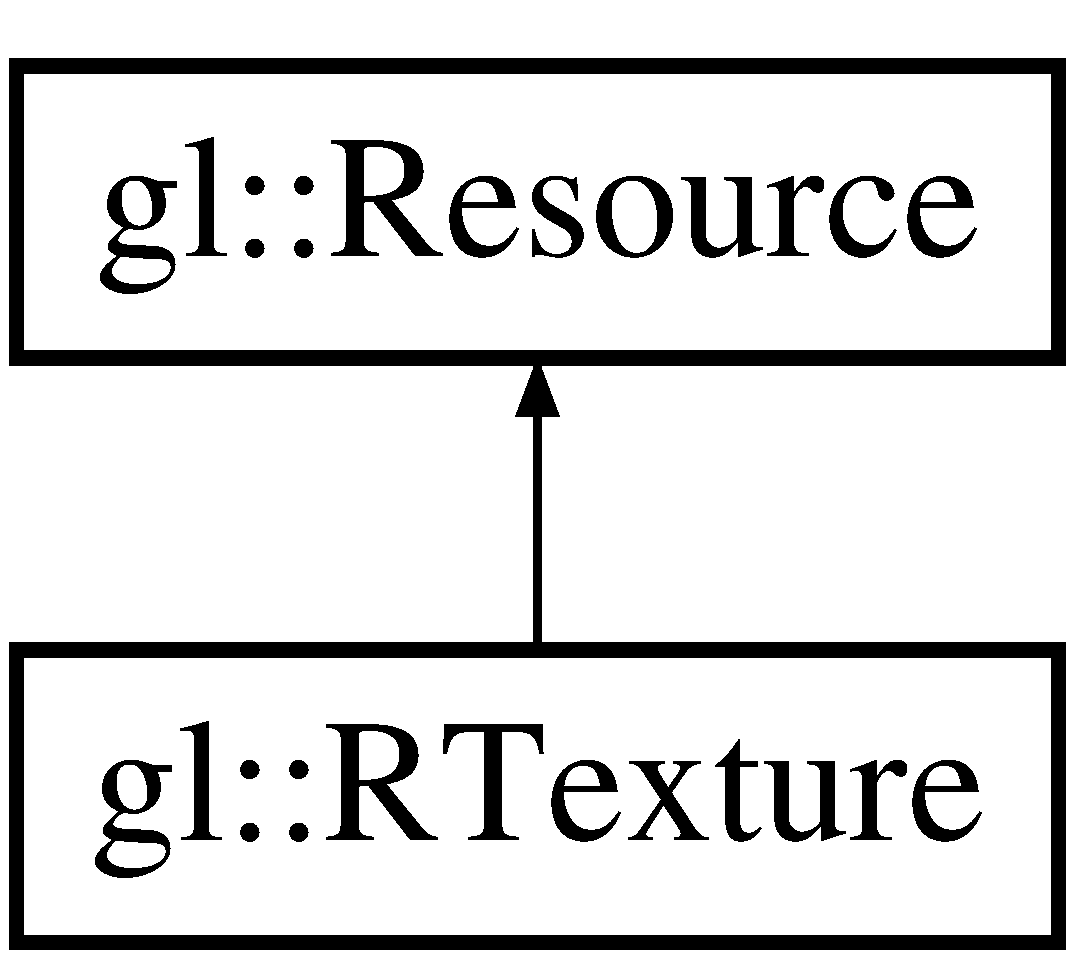
\includegraphics[height=2.000000cm]{classgl_1_1_r_texture}
\end{center}
\end{figure}
\subsection*{Public Types}
\begin{DoxyCompactItemize}
\item 
typedef \hyperlink{classgl_1_1_resource_1_1_configuration}{Resource\-::\-Configuration} \hyperlink{classgl_1_1_r_texture_af5e0de4fdd4b9bd003f8979a07324f0b}{Config\-Type}
\end{DoxyCompactItemize}
\subsection*{Public Member Functions}
\begin{DoxyCompactItemize}
\item 
\hyperlink{classgl_1_1_r_texture_af684b7ee8b937f87938fc3bd211c8345}{R\-Texture} (const \hyperlink{classgl_1_1_resource_1_1_configuration}{Resource\-::\-Configuration} \&config)
\item 
\hyperlink{classgl_1_1_r_texture_a3e1fcfd479e042799893e50b20c2952e}{R\-Texture} (\hyperlink{classgl_1_1_r_texture}{R\-Texture} \&\&other)
\item 
\hyperlink{classgl_1_1_r_texture_a234993b3dfb21867ef249647e233a602}{R\-Texture} (const \hyperlink{classgl_1_1_r_texture}{R\-Texture} \&other)=delete
\item 
\hyperlink{classgl_1_1_r_texture}{R\-Texture} \& \hyperlink{classgl_1_1_r_texture_a6eae2f7e17ebd821d0d3d3b9b2f665f3}{operator=} (const \hyperlink{classgl_1_1_r_texture}{R\-Texture} \&other)=delete
\item 
virtual \hyperlink{classgl_1_1_r_texture_a392daeb25c1bc9fe5d61b8efab97ec42}{$\sim$\-R\-Texture} ()
\item 
G\-Luint \hyperlink{classgl_1_1_r_texture_affea3581b93032c28456eb7a7fe9ffd0}{Get\-Texture\-I\-D} () const 
\item 
\hyperlink{_basic_types_8hpp_afdf0f22c576e6ee1b982f64b839c4bea}{Void} \hyperlink{classgl_1_1_r_texture_a62e2b26cad95a159430c3f61998ac572}{Bind} () const 
\end{DoxyCompactItemize}
\subsection*{Static Public Member Functions}
\begin{DoxyCompactItemize}
\item 
static \hyperlink{_basic_types_8hpp_afdf0f22c576e6ee1b982f64b839c4bea}{Void} \hyperlink{classgl_1_1_r_texture_ab6db1d3aaa5a91ad3cf1fb62348f2a7b}{Bind\-Null} ()
\end{DoxyCompactItemize}
\subsection*{Protected Attributes}
\begin{DoxyCompactItemize}
\item 
G\-Luint \hyperlink{classgl_1_1_r_texture_ac09f29aa4942ab525d65c98217be05ac}{m\-Texture\-I\-D}
\item 
G\-Lenum \hyperlink{classgl_1_1_r_texture_a0442b6e57cd493fa02b2167658785fe4}{m\-Color\-Type}
\end{DoxyCompactItemize}


\subsection{Detailed Description}
\hyperlink{classgl_1_1_r_texture}{R\-Texture} represents a texture for open\-G\-L. Currently it only supports png, more format support in bound. Since \hyperlink{classgl_1_1_r_texture}{R\-Texture} loads the resource itself we need a file name. the default Resource\-Config stores enough info for this. 

Definition at line 25 of file R\-Texture.\-hpp.



\subsection{Member Typedef Documentation}
\hypertarget{classgl_1_1_r_texture_af5e0de4fdd4b9bd003f8979a07324f0b}{\index{gl\-::\-R\-Texture@{gl\-::\-R\-Texture}!Config\-Type@{Config\-Type}}
\index{Config\-Type@{Config\-Type}!gl::RTexture@{gl\-::\-R\-Texture}}
\subsubsection[{Config\-Type}]{\setlength{\rightskip}{0pt plus 5cm}typedef {\bf Resource\-::\-Configuration} {\bf gl\-::\-R\-Texture\-::\-Config\-Type}}}\label{classgl_1_1_r_texture_af5e0de4fdd4b9bd003f8979a07324f0b}


Definition at line 28 of file R\-Texture.\-hpp.



\subsection{Constructor \& Destructor Documentation}
\hypertarget{classgl_1_1_r_texture_af684b7ee8b937f87938fc3bd211c8345}{\index{gl\-::\-R\-Texture@{gl\-::\-R\-Texture}!R\-Texture@{R\-Texture}}
\index{R\-Texture@{R\-Texture}!gl::RTexture@{gl\-::\-R\-Texture}}
\subsubsection[{R\-Texture}]{\setlength{\rightskip}{0pt plus 5cm}gl\-::\-R\-Texture\-::\-R\-Texture (
\begin{DoxyParamCaption}
\item[{const {\bf Resource\-::\-Configuration} \&}]{config}
\end{DoxyParamCaption}
)}}\label{classgl_1_1_r_texture_af684b7ee8b937f87938fc3bd211c8345}


Definition at line 22 of file R\-Texture.\-cpp.

\hypertarget{classgl_1_1_r_texture_a3e1fcfd479e042799893e50b20c2952e}{\index{gl\-::\-R\-Texture@{gl\-::\-R\-Texture}!R\-Texture@{R\-Texture}}
\index{R\-Texture@{R\-Texture}!gl::RTexture@{gl\-::\-R\-Texture}}
\subsubsection[{R\-Texture}]{\setlength{\rightskip}{0pt plus 5cm}gl\-::\-R\-Texture\-::\-R\-Texture (
\begin{DoxyParamCaption}
\item[{{\bf R\-Texture} \&\&}]{other}
\end{DoxyParamCaption}
)}}\label{classgl_1_1_r_texture_a3e1fcfd479e042799893e50b20c2952e}


Definition at line 181 of file R\-Texture.\-cpp.

\hypertarget{classgl_1_1_r_texture_a234993b3dfb21867ef249647e233a602}{\index{gl\-::\-R\-Texture@{gl\-::\-R\-Texture}!R\-Texture@{R\-Texture}}
\index{R\-Texture@{R\-Texture}!gl::RTexture@{gl\-::\-R\-Texture}}
\subsubsection[{R\-Texture}]{\setlength{\rightskip}{0pt plus 5cm}gl\-::\-R\-Texture\-::\-R\-Texture (
\begin{DoxyParamCaption}
\item[{const {\bf R\-Texture} \&}]{other}
\end{DoxyParamCaption}
)\hspace{0.3cm}{\ttfamily [delete]}}}\label{classgl_1_1_r_texture_a234993b3dfb21867ef249647e233a602}
\hypertarget{classgl_1_1_r_texture_a392daeb25c1bc9fe5d61b8efab97ec42}{\index{gl\-::\-R\-Texture@{gl\-::\-R\-Texture}!$\sim$\-R\-Texture@{$\sim$\-R\-Texture}}
\index{$\sim$\-R\-Texture@{$\sim$\-R\-Texture}!gl::RTexture@{gl\-::\-R\-Texture}}
\subsubsection[{$\sim$\-R\-Texture}]{\setlength{\rightskip}{0pt plus 5cm}gl\-::\-R\-Texture\-::$\sim$\-R\-Texture (
\begin{DoxyParamCaption}
{}
\end{DoxyParamCaption}
)\hspace{0.3cm}{\ttfamily [virtual]}}}\label{classgl_1_1_r_texture_a392daeb25c1bc9fe5d61b8efab97ec42}


Definition at line 192 of file R\-Texture.\-cpp.



\subsection{Member Function Documentation}
\hypertarget{classgl_1_1_r_texture_a62e2b26cad95a159430c3f61998ac572}{\index{gl\-::\-R\-Texture@{gl\-::\-R\-Texture}!Bind@{Bind}}
\index{Bind@{Bind}!gl::RTexture@{gl\-::\-R\-Texture}}
\subsubsection[{Bind}]{\setlength{\rightskip}{0pt plus 5cm}{\bf Void} gl\-::\-R\-Texture\-::\-Bind (
\begin{DoxyParamCaption}
{}
\end{DoxyParamCaption}
) const}}\label{classgl_1_1_r_texture_a62e2b26cad95a159430c3f61998ac572}


Definition at line 207 of file R\-Texture.\-cpp.

\hypertarget{classgl_1_1_r_texture_ab6db1d3aaa5a91ad3cf1fb62348f2a7b}{\index{gl\-::\-R\-Texture@{gl\-::\-R\-Texture}!Bind\-Null@{Bind\-Null}}
\index{Bind\-Null@{Bind\-Null}!gl::RTexture@{gl\-::\-R\-Texture}}
\subsubsection[{Bind\-Null}]{\setlength{\rightskip}{0pt plus 5cm}{\bf Void} gl\-::\-R\-Texture\-::\-Bind\-Null (
\begin{DoxyParamCaption}
{}
\end{DoxyParamCaption}
)\hspace{0.3cm}{\ttfamily [static]}}}\label{classgl_1_1_r_texture_ab6db1d3aaa5a91ad3cf1fb62348f2a7b}


Definition at line 212 of file R\-Texture.\-cpp.

\hypertarget{classgl_1_1_r_texture_affea3581b93032c28456eb7a7fe9ffd0}{\index{gl\-::\-R\-Texture@{gl\-::\-R\-Texture}!Get\-Texture\-I\-D@{Get\-Texture\-I\-D}}
\index{Get\-Texture\-I\-D@{Get\-Texture\-I\-D}!gl::RTexture@{gl\-::\-R\-Texture}}
\subsubsection[{Get\-Texture\-I\-D}]{\setlength{\rightskip}{0pt plus 5cm}G\-Luint gl\-::\-R\-Texture\-::\-Get\-Texture\-I\-D (
\begin{DoxyParamCaption}
{}
\end{DoxyParamCaption}
) const}}\label{classgl_1_1_r_texture_affea3581b93032c28456eb7a7fe9ffd0}


Definition at line 202 of file R\-Texture.\-cpp.

\hypertarget{classgl_1_1_r_texture_a6eae2f7e17ebd821d0d3d3b9b2f665f3}{\index{gl\-::\-R\-Texture@{gl\-::\-R\-Texture}!operator=@{operator=}}
\index{operator=@{operator=}!gl::RTexture@{gl\-::\-R\-Texture}}
\subsubsection[{operator=}]{\setlength{\rightskip}{0pt plus 5cm}{\bf R\-Texture}\& gl\-::\-R\-Texture\-::operator= (
\begin{DoxyParamCaption}
\item[{const {\bf R\-Texture} \&}]{other}
\end{DoxyParamCaption}
)\hspace{0.3cm}{\ttfamily [delete]}}}\label{classgl_1_1_r_texture_a6eae2f7e17ebd821d0d3d3b9b2f665f3}


\subsection{Member Data Documentation}
\hypertarget{classgl_1_1_r_texture_a0442b6e57cd493fa02b2167658785fe4}{\index{gl\-::\-R\-Texture@{gl\-::\-R\-Texture}!m\-Color\-Type@{m\-Color\-Type}}
\index{m\-Color\-Type@{m\-Color\-Type}!gl::RTexture@{gl\-::\-R\-Texture}}
\subsubsection[{m\-Color\-Type}]{\setlength{\rightskip}{0pt plus 5cm}G\-Lenum gl\-::\-R\-Texture\-::m\-Color\-Type\hspace{0.3cm}{\ttfamily [protected]}}}\label{classgl_1_1_r_texture_a0442b6e57cd493fa02b2167658785fe4}


Definition at line 54 of file R\-Texture.\-hpp.

\hypertarget{classgl_1_1_r_texture_ac09f29aa4942ab525d65c98217be05ac}{\index{gl\-::\-R\-Texture@{gl\-::\-R\-Texture}!m\-Texture\-I\-D@{m\-Texture\-I\-D}}
\index{m\-Texture\-I\-D@{m\-Texture\-I\-D}!gl::RTexture@{gl\-::\-R\-Texture}}
\subsubsection[{m\-Texture\-I\-D}]{\setlength{\rightskip}{0pt plus 5cm}G\-Luint gl\-::\-R\-Texture\-::m\-Texture\-I\-D\hspace{0.3cm}{\ttfamily [protected]}}}\label{classgl_1_1_r_texture_ac09f29aa4942ab525d65c98217be05ac}


Definition at line 53 of file R\-Texture.\-hpp.



The documentation for this class was generated from the following files\-:\begin{DoxyCompactItemize}
\item 
Glide/\hyperlink{_r_texture_8hpp}{R\-Texture.\-hpp}\item 
Glide/\hyperlink{_r_texture_8cpp}{R\-Texture.\-cpp}\end{DoxyCompactItemize}

\hypertarget{classgl_1_1_scene}{\section{gl\-:\-:Scene Class Reference}
\label{classgl_1_1_scene}\index{gl\-::\-Scene@{gl\-::\-Scene}}
}


{\ttfamily \#include $<$Scene.\-hpp$>$}

\subsection*{Public Member Functions}
\begin{DoxyCompactItemize}
\item 
\hyperlink{classgl_1_1_scene_a20c2bb328c15cc78c5ee9871f8f2533e}{Scene} (const std\-::string \&scene\-File)
\item 
\hyperlink{classgl_1_1_scene_a6ab424422c62cfcae8f9d27568902c89}{$\sim$\-Scene} ()
\item 
\hyperlink{classgl_1_1_game_object}{Game\-Object} $\ast$ \hyperlink{classgl_1_1_scene_a795f1b5059282e416b3ac320df2f6e6b}{Find\-Object\-By\-I\-D} (const std\-::string \&id, \hyperlink{classgl_1_1_game_object}{Game\-Object} $\ast$p\-Start\-Object=nullptr)
\item 
\hyperlink{classgl_1_1_r_shader}{R\-Shader} $\ast$ \hyperlink{classgl_1_1_scene_a67891131153f1b2c47af90743fbc854c}{Get\-Shader} ()
\item 
\hyperlink{_basic_types_8hpp_afdf0f22c576e6ee1b982f64b839c4bea}{Void} \hyperlink{classgl_1_1_scene_a90a883380627b976bebfacc5cc4a24ac}{Render} ()
\end{DoxyCompactItemize}
\subsection*{Protected Member Functions}
\begin{DoxyCompactItemize}
\item 
\hyperlink{_basic_types_8hpp_afdf0f22c576e6ee1b982f64b839c4bea}{Void} \hyperlink{classgl_1_1_scene_abe710b6eb4fcb56b72e4251b30cc007c}{Load\-Materials} (const ai\-Scene $\ast$p\-Scene)
\item 
\hyperlink{_basic_types_8hpp_afdf0f22c576e6ee1b982f64b839c4bea}{Void} \hyperlink{classgl_1_1_scene_aa628ca64f9efc796c5a0977e3db23b1c}{Load\-Meshes} (const ai\-Scene $\ast$p\-Scene)
\item 
\hyperlink{_basic_types_8hpp_afdf0f22c576e6ee1b982f64b839c4bea}{Void} \hyperlink{classgl_1_1_scene_a192e408ea2a6965aab0e8ec1d3923158}{Load\-Nodes} (const ai\-Scene $\ast$p\-Scene)
\item 
\hyperlink{_basic_types_8hpp_afdf0f22c576e6ee1b982f64b839c4bea}{Void} \hyperlink{classgl_1_1_scene_aa1a68b256316296663b03acbba910c6f}{Load\-Node} (const ai\-Node $\ast$p\-Node, \hyperlink{classgl_1_1_game_object}{Game\-Object} $\ast$p\-Parent)
\end{DoxyCompactItemize}
\subsection*{Protected Attributes}
\begin{DoxyCompactItemize}
\item 
\hyperlink{classgl_1_1_resource_manager}{Resource\-Manager}$<$ \hyperlink{classgl_1_1_r_texture}{gl\-::\-R\-Texture}, \\*
std\-::string $>$ \hyperlink{classgl_1_1_scene_a73712112854dd06b3fe837acac4edd26}{m\-Textures}
\item 
\hyperlink{classgl_1_1_resource_manager}{Resource\-Manager}$<$ \hyperlink{classgl_1_1_r_mesh}{gl\-::\-R\-Mesh}, \hyperlink{_basic_types_8hpp_a11c112f01a7ad8f767fd48bc916463a3}{U\-Int} $>$ \hyperlink{classgl_1_1_scene_a4005eea9240f83937897af8798c413c7}{m\-Meshes}
\item 
std\-::unique\-\_\-ptr$<$ \hyperlink{classgl_1_1_r_shader}{R\-Shader} $>$ \hyperlink{classgl_1_1_scene_a8480592c3885010d88253bfcc04d54a0}{mp\-Shader\-Default}
\item 
\hyperlink{namespacegl_a4caed01d7776fc4f8768dbf8d88d0388}{Game\-Object\-Ptr} \hyperlink{classgl_1_1_scene_aaec3924a3fe960cebf42483f8cf163ed}{mp\-Root}
\item 
std\-::string \hyperlink{classgl_1_1_scene_aa81b7ec7e9de4ea30e2d26a3007f35c4}{m\-File}
\end{DoxyCompactItemize}


\subsection{Detailed Description}
Stores the scene node hiarchy, the meshes and textures.

Soon to also store the lights and cameras. 

Definition at line 22 of file Scene.\-hpp.



\subsection{Constructor \& Destructor Documentation}
\hypertarget{classgl_1_1_scene_a20c2bb328c15cc78c5ee9871f8f2533e}{\index{gl\-::\-Scene@{gl\-::\-Scene}!Scene@{Scene}}
\index{Scene@{Scene}!gl::Scene@{gl\-::\-Scene}}
\subsubsection[{Scene}]{\setlength{\rightskip}{0pt plus 5cm}gl\-::\-Scene\-::\-Scene (
\begin{DoxyParamCaption}
\item[{const std\-::string \&}]{scene\-File}
\end{DoxyParamCaption}
)}}\label{classgl_1_1_scene_a20c2bb328c15cc78c5ee9871f8f2533e}


Definition at line 25 of file Scene.\-cpp.

\hypertarget{classgl_1_1_scene_a6ab424422c62cfcae8f9d27568902c89}{\index{gl\-::\-Scene@{gl\-::\-Scene}!$\sim$\-Scene@{$\sim$\-Scene}}
\index{$\sim$\-Scene@{$\sim$\-Scene}!gl::Scene@{gl\-::\-Scene}}
\subsubsection[{$\sim$\-Scene}]{\setlength{\rightskip}{0pt plus 5cm}gl\-::\-Scene\-::$\sim$\-Scene (
\begin{DoxyParamCaption}
{}
\end{DoxyParamCaption}
)}}\label{classgl_1_1_scene_a6ab424422c62cfcae8f9d27568902c89}


Definition at line 50 of file Scene.\-cpp.



\subsection{Member Function Documentation}
\hypertarget{classgl_1_1_scene_a795f1b5059282e416b3ac320df2f6e6b}{\index{gl\-::\-Scene@{gl\-::\-Scene}!Find\-Object\-By\-I\-D@{Find\-Object\-By\-I\-D}}
\index{Find\-Object\-By\-I\-D@{Find\-Object\-By\-I\-D}!gl::Scene@{gl\-::\-Scene}}
\subsubsection[{Find\-Object\-By\-I\-D}]{\setlength{\rightskip}{0pt plus 5cm}{\bf Game\-Object} $\ast$ gl\-::\-Scene\-::\-Find\-Object\-By\-I\-D (
\begin{DoxyParamCaption}
\item[{const std\-::string \&}]{id, }
\item[{{\bf Game\-Object} $\ast$}]{p\-Start\-Object = {\ttfamily nullptr}}
\end{DoxyParamCaption}
)}}\label{classgl_1_1_scene_a795f1b5059282e416b3ac320df2f6e6b}
Get a game object in the hiarchy by its I\-D field. 

Definition at line 223 of file Scene.\-cpp.

\hypertarget{classgl_1_1_scene_a67891131153f1b2c47af90743fbc854c}{\index{gl\-::\-Scene@{gl\-::\-Scene}!Get\-Shader@{Get\-Shader}}
\index{Get\-Shader@{Get\-Shader}!gl::Scene@{gl\-::\-Scene}}
\subsubsection[{Get\-Shader}]{\setlength{\rightskip}{0pt plus 5cm}{\bf R\-Shader} $\ast$ gl\-::\-Scene\-::\-Get\-Shader (
\begin{DoxyParamCaption}
{}
\end{DoxyParamCaption}
)}}\label{classgl_1_1_scene_a67891131153f1b2c47af90743fbc854c}


Definition at line 54 of file Scene.\-cpp.

\hypertarget{classgl_1_1_scene_abe710b6eb4fcb56b72e4251b30cc007c}{\index{gl\-::\-Scene@{gl\-::\-Scene}!Load\-Materials@{Load\-Materials}}
\index{Load\-Materials@{Load\-Materials}!gl::Scene@{gl\-::\-Scene}}
\subsubsection[{Load\-Materials}]{\setlength{\rightskip}{0pt plus 5cm}{\bf Void} gl\-::\-Scene\-::\-Load\-Materials (
\begin{DoxyParamCaption}
\item[{const ai\-Scene $\ast$}]{p\-Scene}
\end{DoxyParamCaption}
)\hspace{0.3cm}{\ttfamily [protected]}}}\label{classgl_1_1_scene_abe710b6eb4fcb56b72e4251b30cc007c}


Definition at line 66 of file Scene.\-cpp.

\hypertarget{classgl_1_1_scene_aa628ca64f9efc796c5a0977e3db23b1c}{\index{gl\-::\-Scene@{gl\-::\-Scene}!Load\-Meshes@{Load\-Meshes}}
\index{Load\-Meshes@{Load\-Meshes}!gl::Scene@{gl\-::\-Scene}}
\subsubsection[{Load\-Meshes}]{\setlength{\rightskip}{0pt plus 5cm}{\bf Void} gl\-::\-Scene\-::\-Load\-Meshes (
\begin{DoxyParamCaption}
\item[{const ai\-Scene $\ast$}]{p\-Scene}
\end{DoxyParamCaption}
)\hspace{0.3cm}{\ttfamily [protected]}}}\label{classgl_1_1_scene_aa628ca64f9efc796c5a0977e3db23b1c}


Definition at line 84 of file Scene.\-cpp.

\hypertarget{classgl_1_1_scene_aa1a68b256316296663b03acbba910c6f}{\index{gl\-::\-Scene@{gl\-::\-Scene}!Load\-Node@{Load\-Node}}
\index{Load\-Node@{Load\-Node}!gl::Scene@{gl\-::\-Scene}}
\subsubsection[{Load\-Node}]{\setlength{\rightskip}{0pt plus 5cm}{\bf Void} gl\-::\-Scene\-::\-Load\-Node (
\begin{DoxyParamCaption}
\item[{const ai\-Node $\ast$}]{p\-Node, }
\item[{{\bf Game\-Object} $\ast$}]{p\-Parent}
\end{DoxyParamCaption}
)\hspace{0.3cm}{\ttfamily [protected]}}}\label{classgl_1_1_scene_aa1a68b256316296663b03acbba910c6f}


Definition at line 177 of file Scene.\-cpp.

\hypertarget{classgl_1_1_scene_a192e408ea2a6965aab0e8ec1d3923158}{\index{gl\-::\-Scene@{gl\-::\-Scene}!Load\-Nodes@{Load\-Nodes}}
\index{Load\-Nodes@{Load\-Nodes}!gl::Scene@{gl\-::\-Scene}}
\subsubsection[{Load\-Nodes}]{\setlength{\rightskip}{0pt plus 5cm}{\bf Void} gl\-::\-Scene\-::\-Load\-Nodes (
\begin{DoxyParamCaption}
\item[{const ai\-Scene $\ast$}]{p\-Scene}
\end{DoxyParamCaption}
)\hspace{0.3cm}{\ttfamily [protected]}}}\label{classgl_1_1_scene_a192e408ea2a6965aab0e8ec1d3923158}


Definition at line 169 of file Scene.\-cpp.

\hypertarget{classgl_1_1_scene_a90a883380627b976bebfacc5cc4a24ac}{\index{gl\-::\-Scene@{gl\-::\-Scene}!Render@{Render}}
\index{Render@{Render}!gl::Scene@{gl\-::\-Scene}}
\subsubsection[{Render}]{\setlength{\rightskip}{0pt plus 5cm}{\bf Void} gl\-::\-Scene\-::\-Render (
\begin{DoxyParamCaption}
{}
\end{DoxyParamCaption}
)}}\label{classgl_1_1_scene_a90a883380627b976bebfacc5cc4a24ac}


Definition at line 59 of file Scene.\-cpp.



\subsection{Member Data Documentation}
\hypertarget{classgl_1_1_scene_aa81b7ec7e9de4ea30e2d26a3007f35c4}{\index{gl\-::\-Scene@{gl\-::\-Scene}!m\-File@{m\-File}}
\index{m\-File@{m\-File}!gl::Scene@{gl\-::\-Scene}}
\subsubsection[{m\-File}]{\setlength{\rightskip}{0pt plus 5cm}std\-::string gl\-::\-Scene\-::m\-File\hspace{0.3cm}{\ttfamily [protected]}}}\label{classgl_1_1_scene_aa81b7ec7e9de4ea30e2d26a3007f35c4}


Definition at line 52 of file Scene.\-hpp.

\hypertarget{classgl_1_1_scene_a4005eea9240f83937897af8798c413c7}{\index{gl\-::\-Scene@{gl\-::\-Scene}!m\-Meshes@{m\-Meshes}}
\index{m\-Meshes@{m\-Meshes}!gl::Scene@{gl\-::\-Scene}}
\subsubsection[{m\-Meshes}]{\setlength{\rightskip}{0pt plus 5cm}{\bf Resource\-Manager}$<$ {\bf gl\-::\-R\-Mesh}, {\bf U\-Int} $>$ gl\-::\-Scene\-::m\-Meshes\hspace{0.3cm}{\ttfamily [protected]}}}\label{classgl_1_1_scene_a4005eea9240f83937897af8798c413c7}


Definition at line 46 of file Scene.\-hpp.

\hypertarget{classgl_1_1_scene_aaec3924a3fe960cebf42483f8cf163ed}{\index{gl\-::\-Scene@{gl\-::\-Scene}!mp\-Root@{mp\-Root}}
\index{mp\-Root@{mp\-Root}!gl::Scene@{gl\-::\-Scene}}
\subsubsection[{mp\-Root}]{\setlength{\rightskip}{0pt plus 5cm}{\bf Game\-Object\-Ptr} gl\-::\-Scene\-::mp\-Root\hspace{0.3cm}{\ttfamily [protected]}}}\label{classgl_1_1_scene_aaec3924a3fe960cebf42483f8cf163ed}


Definition at line 50 of file Scene.\-hpp.

\hypertarget{classgl_1_1_scene_a8480592c3885010d88253bfcc04d54a0}{\index{gl\-::\-Scene@{gl\-::\-Scene}!mp\-Shader\-Default@{mp\-Shader\-Default}}
\index{mp\-Shader\-Default@{mp\-Shader\-Default}!gl::Scene@{gl\-::\-Scene}}
\subsubsection[{mp\-Shader\-Default}]{\setlength{\rightskip}{0pt plus 5cm}std\-::unique\-\_\-ptr$<${\bf R\-Shader}$>$ gl\-::\-Scene\-::mp\-Shader\-Default\hspace{0.3cm}{\ttfamily [protected]}}}\label{classgl_1_1_scene_a8480592c3885010d88253bfcc04d54a0}


Definition at line 48 of file Scene.\-hpp.

\hypertarget{classgl_1_1_scene_a73712112854dd06b3fe837acac4edd26}{\index{gl\-::\-Scene@{gl\-::\-Scene}!m\-Textures@{m\-Textures}}
\index{m\-Textures@{m\-Textures}!gl::Scene@{gl\-::\-Scene}}
\subsubsection[{m\-Textures}]{\setlength{\rightskip}{0pt plus 5cm}{\bf Resource\-Manager}$<$ {\bf gl\-::\-R\-Texture}, std\-::string $>$ gl\-::\-Scene\-::m\-Textures\hspace{0.3cm}{\ttfamily [protected]}}}\label{classgl_1_1_scene_a73712112854dd06b3fe837acac4edd26}


Definition at line 45 of file Scene.\-hpp.



The documentation for this class was generated from the following files\-:\begin{DoxyCompactItemize}
\item 
Glide/\hyperlink{_scene_8hpp}{Scene.\-hpp}\item 
Glide/\hyperlink{_scene_8cpp}{Scene.\-cpp}\end{DoxyCompactItemize}

\hypertarget{classtinyxml2_1_1_str_pair}{\section{tinyxml2\-:\-:Str\-Pair Class Reference}
\label{classtinyxml2_1_1_str_pair}\index{tinyxml2\-::\-Str\-Pair@{tinyxml2\-::\-Str\-Pair}}
}


{\ttfamily \#include $<$tinyxml2.\-hpp$>$}

\subsection*{Public Types}
\begin{DoxyCompactItemize}
\item 
enum \{ \\*
\hyperlink{classtinyxml2_1_1_str_pair_a0301ef962e15dd94574431f1c61266c5a4f1e01a55f8efe4ca72c32d454060237}{N\-E\-E\-D\-S\-\_\-\-E\-N\-T\-I\-T\-Y\-\_\-\-P\-R\-O\-C\-E\-S\-S\-I\-N\-G} = 0x01, 
\hyperlink{classtinyxml2_1_1_str_pair_a0301ef962e15dd94574431f1c61266c5a8f2045d56e70745d718672c0da91d0e0}{N\-E\-E\-D\-S\-\_\-\-N\-E\-W\-L\-I\-N\-E\-\_\-\-N\-O\-R\-M\-A\-L\-I\-Z\-A\-T\-I\-O\-N} = 0x02, 
\hyperlink{classtinyxml2_1_1_str_pair_a0301ef962e15dd94574431f1c61266c5ab17a85f396c221811fe49263bf6f843f}{C\-O\-L\-L\-A\-P\-S\-E\-\_\-\-W\-H\-I\-T\-E\-S\-P\-A\-C\-E} = 0x04, 
\hyperlink{classtinyxml2_1_1_str_pair_a0301ef962e15dd94574431f1c61266c5aae519eb5a639858591763aa5fc6cc953}{T\-E\-X\-T\-\_\-\-E\-L\-E\-M\-E\-N\-T} = N\-E\-E\-D\-S\-\_\-\-E\-N\-T\-I\-T\-Y\-\_\-\-P\-R\-O\-C\-E\-S\-S\-I\-N\-G $\vert$ N\-E\-E\-D\-S\-\_\-\-N\-E\-W\-L\-I\-N\-E\-\_\-\-N\-O\-R\-M\-A\-L\-I\-Z\-A\-T\-I\-O\-N, 
\\*
\hyperlink{classtinyxml2_1_1_str_pair_a0301ef962e15dd94574431f1c61266c5a96be48cf899bfeea0aa227f984f1fa63}{T\-E\-X\-T\-\_\-\-E\-L\-E\-M\-E\-N\-T\-\_\-\-L\-E\-A\-V\-E\-\_\-\-E\-N\-T\-I\-T\-I\-E\-S} = N\-E\-E\-D\-S\-\_\-\-N\-E\-W\-L\-I\-N\-E\-\_\-\-N\-O\-R\-M\-A\-L\-I\-Z\-A\-T\-I\-O\-N, 
\hyperlink{classtinyxml2_1_1_str_pair_a0301ef962e15dd94574431f1c61266c5aaab1cbefaa977e6f772b4e2575417aeb}{A\-T\-T\-R\-I\-B\-U\-T\-E\-\_\-\-N\-A\-M\-E} = 0, 
\hyperlink{classtinyxml2_1_1_str_pair_a0301ef962e15dd94574431f1c61266c5a6d72f9ce15f50e8bcd680edf66235dfd}{A\-T\-T\-R\-I\-B\-U\-T\-E\-\_\-\-V\-A\-L\-U\-E} = N\-E\-E\-D\-S\-\_\-\-E\-N\-T\-I\-T\-Y\-\_\-\-P\-R\-O\-C\-E\-S\-S\-I\-N\-G $\vert$ N\-E\-E\-D\-S\-\_\-\-N\-E\-W\-L\-I\-N\-E\-\_\-\-N\-O\-R\-M\-A\-L\-I\-Z\-A\-T\-I\-O\-N, 
\hyperlink{classtinyxml2_1_1_str_pair_a0301ef962e15dd94574431f1c61266c5a2decbd2513ac14f8befa987938326399}{A\-T\-T\-R\-I\-B\-U\-T\-E\-\_\-\-V\-A\-L\-U\-E\-\_\-\-L\-E\-A\-V\-E\-\_\-\-E\-N\-T\-I\-T\-I\-E\-S} = N\-E\-E\-D\-S\-\_\-\-N\-E\-W\-L\-I\-N\-E\-\_\-\-N\-O\-R\-M\-A\-L\-I\-Z\-A\-T\-I\-O\-N, 
\\*
\hyperlink{classtinyxml2_1_1_str_pair_a0301ef962e15dd94574431f1c61266c5a067a6ec90c8beea1cf5992930d93bffa}{C\-O\-M\-M\-E\-N\-T} = N\-E\-E\-D\-S\-\_\-\-N\-E\-W\-L\-I\-N\-E\-\_\-\-N\-O\-R\-M\-A\-L\-I\-Z\-A\-T\-I\-O\-N
 \}
\end{DoxyCompactItemize}
\subsection*{Public Member Functions}
\begin{DoxyCompactItemize}
\item 
\hyperlink{classtinyxml2_1_1_str_pair_a69153963f7052de9f767d3d8c1623a70}{Str\-Pair} ()
\item 
\hyperlink{classtinyxml2_1_1_str_pair_a60bed84d2503296e1c2a73fcef1431f9}{$\sim$\-Str\-Pair} ()
\item 
void \hyperlink{classtinyxml2_1_1_str_pair_a4f05549373394266a1eecba26813c166}{Set} (char $\ast$start, char $\ast$end, int flags)
\item 
const char $\ast$ \hyperlink{classtinyxml2_1_1_str_pair_ad87e3d11330f5e689ba1e7e54c023b57}{Get\-Str} ()
\item 
bool \hyperlink{classtinyxml2_1_1_str_pair_affa1043e73a18f05d5d2faec055725a7}{Empty} () const 
\item 
void \hyperlink{classtinyxml2_1_1_str_pair_a2baf6230e18333e02ab65d0897ee3941}{Set\-Interned\-Str} (const char $\ast$str)
\item 
void \hyperlink{classtinyxml2_1_1_str_pair_a1f82ec6b5bee35ee7466d8565e43b1de}{Set\-Str} (const char $\ast$str, int flags=0)
\item 
char $\ast$ \hyperlink{classtinyxml2_1_1_str_pair_ad90521f188e9606a8fbafe5d86fb2246}{Parse\-Text} (char $\ast$in, const char $\ast$end\-Tag, int str\-Flags)
\item 
char $\ast$ \hyperlink{classtinyxml2_1_1_str_pair_aa6d8998efceba41d87ec2300c70a6085}{Parse\-Name} (char $\ast$in)
\end{DoxyCompactItemize}


\subsection{Detailed Description}


Definition at line 140 of file tinyxml2.\-hpp.



\subsection{Member Enumeration Documentation}
\hypertarget{classtinyxml2_1_1_str_pair_a0301ef962e15dd94574431f1c61266c5}{\subsubsection[{anonymous enum}]{\setlength{\rightskip}{0pt plus 5cm}anonymous enum}}\label{classtinyxml2_1_1_str_pair_a0301ef962e15dd94574431f1c61266c5}
\begin{Desc}
\item[Enumerator]\par
\begin{description}
\index{N\-E\-E\-D\-S\-\_\-\-E\-N\-T\-I\-T\-Y\-\_\-\-P\-R\-O\-C\-E\-S\-S\-I\-N\-G@{N\-E\-E\-D\-S\-\_\-\-E\-N\-T\-I\-T\-Y\-\_\-\-P\-R\-O\-C\-E\-S\-S\-I\-N\-G}!tinyxml2\-::\-Str\-Pair@{tinyxml2\-::\-Str\-Pair}}\index{tinyxml2\-::\-Str\-Pair@{tinyxml2\-::\-Str\-Pair}!N\-E\-E\-D\-S\-\_\-\-E\-N\-T\-I\-T\-Y\-\_\-\-P\-R\-O\-C\-E\-S\-S\-I\-N\-G@{N\-E\-E\-D\-S\-\_\-\-E\-N\-T\-I\-T\-Y\-\_\-\-P\-R\-O\-C\-E\-S\-S\-I\-N\-G}}\item[{\em 
\hypertarget{classtinyxml2_1_1_str_pair_a0301ef962e15dd94574431f1c61266c5a4f1e01a55f8efe4ca72c32d454060237}{N\-E\-E\-D\-S\-\_\-\-E\-N\-T\-I\-T\-Y\-\_\-\-P\-R\-O\-C\-E\-S\-S\-I\-N\-G}\label{classtinyxml2_1_1_str_pair_a0301ef962e15dd94574431f1c61266c5a4f1e01a55f8efe4ca72c32d454060237}
}]\index{N\-E\-E\-D\-S\-\_\-\-N\-E\-W\-L\-I\-N\-E\-\_\-\-N\-O\-R\-M\-A\-L\-I\-Z\-A\-T\-I\-O\-N@{N\-E\-E\-D\-S\-\_\-\-N\-E\-W\-L\-I\-N\-E\-\_\-\-N\-O\-R\-M\-A\-L\-I\-Z\-A\-T\-I\-O\-N}!tinyxml2\-::\-Str\-Pair@{tinyxml2\-::\-Str\-Pair}}\index{tinyxml2\-::\-Str\-Pair@{tinyxml2\-::\-Str\-Pair}!N\-E\-E\-D\-S\-\_\-\-N\-E\-W\-L\-I\-N\-E\-\_\-\-N\-O\-R\-M\-A\-L\-I\-Z\-A\-T\-I\-O\-N@{N\-E\-E\-D\-S\-\_\-\-N\-E\-W\-L\-I\-N\-E\-\_\-\-N\-O\-R\-M\-A\-L\-I\-Z\-A\-T\-I\-O\-N}}\item[{\em 
\hypertarget{classtinyxml2_1_1_str_pair_a0301ef962e15dd94574431f1c61266c5a8f2045d56e70745d718672c0da91d0e0}{N\-E\-E\-D\-S\-\_\-\-N\-E\-W\-L\-I\-N\-E\-\_\-\-N\-O\-R\-M\-A\-L\-I\-Z\-A\-T\-I\-O\-N}\label{classtinyxml2_1_1_str_pair_a0301ef962e15dd94574431f1c61266c5a8f2045d56e70745d718672c0da91d0e0}
}]\index{C\-O\-L\-L\-A\-P\-S\-E\-\_\-\-W\-H\-I\-T\-E\-S\-P\-A\-C\-E@{C\-O\-L\-L\-A\-P\-S\-E\-\_\-\-W\-H\-I\-T\-E\-S\-P\-A\-C\-E}!tinyxml2\-::\-Str\-Pair@{tinyxml2\-::\-Str\-Pair}}\index{tinyxml2\-::\-Str\-Pair@{tinyxml2\-::\-Str\-Pair}!C\-O\-L\-L\-A\-P\-S\-E\-\_\-\-W\-H\-I\-T\-E\-S\-P\-A\-C\-E@{C\-O\-L\-L\-A\-P\-S\-E\-\_\-\-W\-H\-I\-T\-E\-S\-P\-A\-C\-E}}\item[{\em 
\hypertarget{classtinyxml2_1_1_str_pair_a0301ef962e15dd94574431f1c61266c5ab17a85f396c221811fe49263bf6f843f}{C\-O\-L\-L\-A\-P\-S\-E\-\_\-\-W\-H\-I\-T\-E\-S\-P\-A\-C\-E}\label{classtinyxml2_1_1_str_pair_a0301ef962e15dd94574431f1c61266c5ab17a85f396c221811fe49263bf6f843f}
}]\index{T\-E\-X\-T\-\_\-\-E\-L\-E\-M\-E\-N\-T@{T\-E\-X\-T\-\_\-\-E\-L\-E\-M\-E\-N\-T}!tinyxml2\-::\-Str\-Pair@{tinyxml2\-::\-Str\-Pair}}\index{tinyxml2\-::\-Str\-Pair@{tinyxml2\-::\-Str\-Pair}!T\-E\-X\-T\-\_\-\-E\-L\-E\-M\-E\-N\-T@{T\-E\-X\-T\-\_\-\-E\-L\-E\-M\-E\-N\-T}}\item[{\em 
\hypertarget{classtinyxml2_1_1_str_pair_a0301ef962e15dd94574431f1c61266c5aae519eb5a639858591763aa5fc6cc953}{T\-E\-X\-T\-\_\-\-E\-L\-E\-M\-E\-N\-T}\label{classtinyxml2_1_1_str_pair_a0301ef962e15dd94574431f1c61266c5aae519eb5a639858591763aa5fc6cc953}
}]\index{T\-E\-X\-T\-\_\-\-E\-L\-E\-M\-E\-N\-T\-\_\-\-L\-E\-A\-V\-E\-\_\-\-E\-N\-T\-I\-T\-I\-E\-S@{T\-E\-X\-T\-\_\-\-E\-L\-E\-M\-E\-N\-T\-\_\-\-L\-E\-A\-V\-E\-\_\-\-E\-N\-T\-I\-T\-I\-E\-S}!tinyxml2\-::\-Str\-Pair@{tinyxml2\-::\-Str\-Pair}}\index{tinyxml2\-::\-Str\-Pair@{tinyxml2\-::\-Str\-Pair}!T\-E\-X\-T\-\_\-\-E\-L\-E\-M\-E\-N\-T\-\_\-\-L\-E\-A\-V\-E\-\_\-\-E\-N\-T\-I\-T\-I\-E\-S@{T\-E\-X\-T\-\_\-\-E\-L\-E\-M\-E\-N\-T\-\_\-\-L\-E\-A\-V\-E\-\_\-\-E\-N\-T\-I\-T\-I\-E\-S}}\item[{\em 
\hypertarget{classtinyxml2_1_1_str_pair_a0301ef962e15dd94574431f1c61266c5a96be48cf899bfeea0aa227f984f1fa63}{T\-E\-X\-T\-\_\-\-E\-L\-E\-M\-E\-N\-T\-\_\-\-L\-E\-A\-V\-E\-\_\-\-E\-N\-T\-I\-T\-I\-E\-S}\label{classtinyxml2_1_1_str_pair_a0301ef962e15dd94574431f1c61266c5a96be48cf899bfeea0aa227f984f1fa63}
}]\index{A\-T\-T\-R\-I\-B\-U\-T\-E\-\_\-\-N\-A\-M\-E@{A\-T\-T\-R\-I\-B\-U\-T\-E\-\_\-\-N\-A\-M\-E}!tinyxml2\-::\-Str\-Pair@{tinyxml2\-::\-Str\-Pair}}\index{tinyxml2\-::\-Str\-Pair@{tinyxml2\-::\-Str\-Pair}!A\-T\-T\-R\-I\-B\-U\-T\-E\-\_\-\-N\-A\-M\-E@{A\-T\-T\-R\-I\-B\-U\-T\-E\-\_\-\-N\-A\-M\-E}}\item[{\em 
\hypertarget{classtinyxml2_1_1_str_pair_a0301ef962e15dd94574431f1c61266c5aaab1cbefaa977e6f772b4e2575417aeb}{A\-T\-T\-R\-I\-B\-U\-T\-E\-\_\-\-N\-A\-M\-E}\label{classtinyxml2_1_1_str_pair_a0301ef962e15dd94574431f1c61266c5aaab1cbefaa977e6f772b4e2575417aeb}
}]\index{A\-T\-T\-R\-I\-B\-U\-T\-E\-\_\-\-V\-A\-L\-U\-E@{A\-T\-T\-R\-I\-B\-U\-T\-E\-\_\-\-V\-A\-L\-U\-E}!tinyxml2\-::\-Str\-Pair@{tinyxml2\-::\-Str\-Pair}}\index{tinyxml2\-::\-Str\-Pair@{tinyxml2\-::\-Str\-Pair}!A\-T\-T\-R\-I\-B\-U\-T\-E\-\_\-\-V\-A\-L\-U\-E@{A\-T\-T\-R\-I\-B\-U\-T\-E\-\_\-\-V\-A\-L\-U\-E}}\item[{\em 
\hypertarget{classtinyxml2_1_1_str_pair_a0301ef962e15dd94574431f1c61266c5a6d72f9ce15f50e8bcd680edf66235dfd}{A\-T\-T\-R\-I\-B\-U\-T\-E\-\_\-\-V\-A\-L\-U\-E}\label{classtinyxml2_1_1_str_pair_a0301ef962e15dd94574431f1c61266c5a6d72f9ce15f50e8bcd680edf66235dfd}
}]\index{A\-T\-T\-R\-I\-B\-U\-T\-E\-\_\-\-V\-A\-L\-U\-E\-\_\-\-L\-E\-A\-V\-E\-\_\-\-E\-N\-T\-I\-T\-I\-E\-S@{A\-T\-T\-R\-I\-B\-U\-T\-E\-\_\-\-V\-A\-L\-U\-E\-\_\-\-L\-E\-A\-V\-E\-\_\-\-E\-N\-T\-I\-T\-I\-E\-S}!tinyxml2\-::\-Str\-Pair@{tinyxml2\-::\-Str\-Pair}}\index{tinyxml2\-::\-Str\-Pair@{tinyxml2\-::\-Str\-Pair}!A\-T\-T\-R\-I\-B\-U\-T\-E\-\_\-\-V\-A\-L\-U\-E\-\_\-\-L\-E\-A\-V\-E\-\_\-\-E\-N\-T\-I\-T\-I\-E\-S@{A\-T\-T\-R\-I\-B\-U\-T\-E\-\_\-\-V\-A\-L\-U\-E\-\_\-\-L\-E\-A\-V\-E\-\_\-\-E\-N\-T\-I\-T\-I\-E\-S}}\item[{\em 
\hypertarget{classtinyxml2_1_1_str_pair_a0301ef962e15dd94574431f1c61266c5a2decbd2513ac14f8befa987938326399}{A\-T\-T\-R\-I\-B\-U\-T\-E\-\_\-\-V\-A\-L\-U\-E\-\_\-\-L\-E\-A\-V\-E\-\_\-\-E\-N\-T\-I\-T\-I\-E\-S}\label{classtinyxml2_1_1_str_pair_a0301ef962e15dd94574431f1c61266c5a2decbd2513ac14f8befa987938326399}
}]\index{C\-O\-M\-M\-E\-N\-T@{C\-O\-M\-M\-E\-N\-T}!tinyxml2\-::\-Str\-Pair@{tinyxml2\-::\-Str\-Pair}}\index{tinyxml2\-::\-Str\-Pair@{tinyxml2\-::\-Str\-Pair}!C\-O\-M\-M\-E\-N\-T@{C\-O\-M\-M\-E\-N\-T}}\item[{\em 
\hypertarget{classtinyxml2_1_1_str_pair_a0301ef962e15dd94574431f1c61266c5a067a6ec90c8beea1cf5992930d93bffa}{C\-O\-M\-M\-E\-N\-T}\label{classtinyxml2_1_1_str_pair_a0301ef962e15dd94574431f1c61266c5a067a6ec90c8beea1cf5992930d93bffa}
}]\end{description}
\end{Desc}


Definition at line 143 of file tinyxml2.\-hpp.



\subsection{Constructor \& Destructor Documentation}
\hypertarget{classtinyxml2_1_1_str_pair_a69153963f7052de9f767d3d8c1623a70}{\index{tinyxml2\-::\-Str\-Pair@{tinyxml2\-::\-Str\-Pair}!Str\-Pair@{Str\-Pair}}
\index{Str\-Pair@{Str\-Pair}!tinyxml2::StrPair@{tinyxml2\-::\-Str\-Pair}}
\subsubsection[{Str\-Pair}]{\setlength{\rightskip}{0pt plus 5cm}tinyxml2\-::\-Str\-Pair\-::\-Str\-Pair (
\begin{DoxyParamCaption}
{}
\end{DoxyParamCaption}
)\hspace{0.3cm}{\ttfamily [inline]}}}\label{classtinyxml2_1_1_str_pair_a69153963f7052de9f767d3d8c1623a70}


Definition at line 156 of file tinyxml2.\-hpp.

\hypertarget{classtinyxml2_1_1_str_pair_a60bed84d2503296e1c2a73fcef1431f9}{\index{tinyxml2\-::\-Str\-Pair@{tinyxml2\-::\-Str\-Pair}!$\sim$\-Str\-Pair@{$\sim$\-Str\-Pair}}
\index{$\sim$\-Str\-Pair@{$\sim$\-Str\-Pair}!tinyxml2::StrPair@{tinyxml2\-::\-Str\-Pair}}
\subsubsection[{$\sim$\-Str\-Pair}]{\setlength{\rightskip}{0pt plus 5cm}tinyxml2\-::\-Str\-Pair\-::$\sim$\-Str\-Pair (
\begin{DoxyParamCaption}
{}
\end{DoxyParamCaption}
)}}\label{classtinyxml2_1_1_str_pair_a60bed84d2503296e1c2a73fcef1431f9}


Definition at line 83 of file tinyxml2.\-cpp.



\subsection{Member Function Documentation}
\hypertarget{classtinyxml2_1_1_str_pair_affa1043e73a18f05d5d2faec055725a7}{\index{tinyxml2\-::\-Str\-Pair@{tinyxml2\-::\-Str\-Pair}!Empty@{Empty}}
\index{Empty@{Empty}!tinyxml2::StrPair@{tinyxml2\-::\-Str\-Pair}}
\subsubsection[{Empty}]{\setlength{\rightskip}{0pt plus 5cm}bool tinyxml2\-::\-Str\-Pair\-::\-Empty (
\begin{DoxyParamCaption}
{}
\end{DoxyParamCaption}
) const\hspace{0.3cm}{\ttfamily [inline]}}}\label{classtinyxml2_1_1_str_pair_affa1043e73a18f05d5d2faec055725a7}


Definition at line 168 of file tinyxml2.\-hpp.

\hypertarget{classtinyxml2_1_1_str_pair_ad87e3d11330f5e689ba1e7e54c023b57}{\index{tinyxml2\-::\-Str\-Pair@{tinyxml2\-::\-Str\-Pair}!Get\-Str@{Get\-Str}}
\index{Get\-Str@{Get\-Str}!tinyxml2::StrPair@{tinyxml2\-::\-Str\-Pair}}
\subsubsection[{Get\-Str}]{\setlength{\rightskip}{0pt plus 5cm}const char $\ast$ tinyxml2\-::\-Str\-Pair\-::\-Get\-Str (
\begin{DoxyParamCaption}
{}
\end{DoxyParamCaption}
)}}\label{classtinyxml2_1_1_str_pair_ad87e3d11330f5e689ba1e7e54c023b57}


Definition at line 178 of file tinyxml2.\-cpp.

\hypertarget{classtinyxml2_1_1_str_pair_aa6d8998efceba41d87ec2300c70a6085}{\index{tinyxml2\-::\-Str\-Pair@{tinyxml2\-::\-Str\-Pair}!Parse\-Name@{Parse\-Name}}
\index{Parse\-Name@{Parse\-Name}!tinyxml2::StrPair@{tinyxml2\-::\-Str\-Pair}}
\subsubsection[{Parse\-Name}]{\setlength{\rightskip}{0pt plus 5cm}char $\ast$ tinyxml2\-::\-Str\-Pair\-::\-Parse\-Name (
\begin{DoxyParamCaption}
\item[{char $\ast$}]{in}
\end{DoxyParamCaption}
)}}\label{classtinyxml2_1_1_str_pair_aa6d8998efceba41d87ec2300c70a6085}


Definition at line 131 of file tinyxml2.\-cpp.

\hypertarget{classtinyxml2_1_1_str_pair_ad90521f188e9606a8fbafe5d86fb2246}{\index{tinyxml2\-::\-Str\-Pair@{tinyxml2\-::\-Str\-Pair}!Parse\-Text@{Parse\-Text}}
\index{Parse\-Text@{Parse\-Text}!tinyxml2::StrPair@{tinyxml2\-::\-Str\-Pair}}
\subsubsection[{Parse\-Text}]{\setlength{\rightskip}{0pt plus 5cm}char $\ast$ tinyxml2\-::\-Str\-Pair\-::\-Parse\-Text (
\begin{DoxyParamCaption}
\item[{char $\ast$}]{in, }
\item[{const char $\ast$}]{end\-Tag, }
\item[{int}]{str\-Flags}
\end{DoxyParamCaption}
)}}\label{classtinyxml2_1_1_str_pair_ad90521f188e9606a8fbafe5d86fb2246}


Definition at line 111 of file tinyxml2.\-cpp.

\hypertarget{classtinyxml2_1_1_str_pair_a4f05549373394266a1eecba26813c166}{\index{tinyxml2\-::\-Str\-Pair@{tinyxml2\-::\-Str\-Pair}!Set@{Set}}
\index{Set@{Set}!tinyxml2::StrPair@{tinyxml2\-::\-Str\-Pair}}
\subsubsection[{Set}]{\setlength{\rightskip}{0pt plus 5cm}void tinyxml2\-::\-Str\-Pair\-::\-Set (
\begin{DoxyParamCaption}
\item[{char $\ast$}]{start, }
\item[{char $\ast$}]{end, }
\item[{int}]{flags}
\end{DoxyParamCaption}
)\hspace{0.3cm}{\ttfamily [inline]}}}\label{classtinyxml2_1_1_str_pair_a4f05549373394266a1eecba26813c166}


Definition at line 159 of file tinyxml2.\-hpp.

\hypertarget{classtinyxml2_1_1_str_pair_a2baf6230e18333e02ab65d0897ee3941}{\index{tinyxml2\-::\-Str\-Pair@{tinyxml2\-::\-Str\-Pair}!Set\-Interned\-Str@{Set\-Interned\-Str}}
\index{Set\-Interned\-Str@{Set\-Interned\-Str}!tinyxml2::StrPair@{tinyxml2\-::\-Str\-Pair}}
\subsubsection[{Set\-Interned\-Str}]{\setlength{\rightskip}{0pt plus 5cm}void tinyxml2\-::\-Str\-Pair\-::\-Set\-Interned\-Str (
\begin{DoxyParamCaption}
\item[{const char $\ast$}]{str}
\end{DoxyParamCaption}
)\hspace{0.3cm}{\ttfamily [inline]}}}\label{classtinyxml2_1_1_str_pair_a2baf6230e18333e02ab65d0897ee3941}


Definition at line 172 of file tinyxml2.\-hpp.

\hypertarget{classtinyxml2_1_1_str_pair_a1f82ec6b5bee35ee7466d8565e43b1de}{\index{tinyxml2\-::\-Str\-Pair@{tinyxml2\-::\-Str\-Pair}!Set\-Str@{Set\-Str}}
\index{Set\-Str@{Set\-Str}!tinyxml2::StrPair@{tinyxml2\-::\-Str\-Pair}}
\subsubsection[{Set\-Str}]{\setlength{\rightskip}{0pt plus 5cm}void tinyxml2\-::\-Str\-Pair\-::\-Set\-Str (
\begin{DoxyParamCaption}
\item[{const char $\ast$}]{str, }
\item[{int}]{flags = {\ttfamily 0}}
\end{DoxyParamCaption}
)}}\label{classtinyxml2_1_1_str_pair_a1f82ec6b5bee35ee7466d8565e43b1de}


Definition at line 100 of file tinyxml2.\-cpp.



The documentation for this class was generated from the following files\-:\begin{DoxyCompactItemize}
\item 
Glide/\hyperlink{tinyxml2_8hpp}{tinyxml2.\-hpp}\item 
Glide/\hyperlink{tinyxml2_8cpp}{tinyxml2.\-cpp}\end{DoxyCompactItemize}

\hypertarget{classtinyxml2_1_1_x_m_l_attribute}{\section{tinyxml2\-:\-:X\-M\-L\-Attribute Class Reference}
\label{classtinyxml2_1_1_x_m_l_attribute}\index{tinyxml2\-::\-X\-M\-L\-Attribute@{tinyxml2\-::\-X\-M\-L\-Attribute}}
}


{\ttfamily \#include $<$tinyxml2.\-hpp$>$}

\subsection*{Public Member Functions}
\begin{DoxyCompactItemize}
\item 
const char $\ast$ \hyperlink{classtinyxml2_1_1_x_m_l_attribute_a631990ac0d176e38fc291b17b295a62d}{Name} () const 
\begin{DoxyCompactList}\small\item\em The name of the attribute. \end{DoxyCompactList}\item 
const char $\ast$ \hyperlink{classtinyxml2_1_1_x_m_l_attribute_adf884db24f469f8a99a14ae786d4ddd7}{Value} () const 
\begin{DoxyCompactList}\small\item\em The value of the attribute. \end{DoxyCompactList}\item 
const \hyperlink{classtinyxml2_1_1_x_m_l_attribute}{X\-M\-L\-Attribute} $\ast$ \hyperlink{classtinyxml2_1_1_x_m_l_attribute_a7fd852d6185af90361ec1bc9a7681ad6}{Next} () const 
\begin{DoxyCompactList}\small\item\em The next attribute in the list. \end{DoxyCompactList}\item 
int \hyperlink{classtinyxml2_1_1_x_m_l_attribute_a949d02a5888092cc68c1e29185301863}{Int\-Value} () const 
\item 
unsigned \hyperlink{classtinyxml2_1_1_x_m_l_attribute_a4c7a179907836a136d1ce5acbe53389d}{Unsigned\-Value} () const 
\begin{DoxyCompactList}\small\item\em Query as an unsigned integer. See \hyperlink{classtinyxml2_1_1_x_m_l_attribute_a949d02a5888092cc68c1e29185301863}{Int\-Value()} \end{DoxyCompactList}\item 
bool \hyperlink{classtinyxml2_1_1_x_m_l_attribute_afb444b7a12527f836aa161b54b2f7ce7}{Bool\-Value} () const 
\begin{DoxyCompactList}\small\item\em Query as a boolean. See \hyperlink{classtinyxml2_1_1_x_m_l_attribute_a949d02a5888092cc68c1e29185301863}{Int\-Value()} \end{DoxyCompactList}\item 
double \hyperlink{classtinyxml2_1_1_x_m_l_attribute_a336153e5aa1b7ccd6502fc249bfb3fd7}{Double\-Value} () const 
\begin{DoxyCompactList}\small\item\em Query as a double. See \hyperlink{classtinyxml2_1_1_x_m_l_attribute_a949d02a5888092cc68c1e29185301863}{Int\-Value()} \end{DoxyCompactList}\item 
float \hyperlink{classtinyxml2_1_1_x_m_l_attribute_ae3d51ff98eacc1dc46efcfdaee5c84ad}{Float\-Value} () const 
\begin{DoxyCompactList}\small\item\em Query as a float. See \hyperlink{classtinyxml2_1_1_x_m_l_attribute_a949d02a5888092cc68c1e29185301863}{Int\-Value()} \end{DoxyCompactList}\item 
\hyperlink{namespacetinyxml2_a1fbf88509c3ac88c09117b1947414e08}{X\-M\-L\-Error} \hyperlink{classtinyxml2_1_1_x_m_l_attribute_ad510a83c4ff2755844bb250b125d28ff}{Query\-Int\-Value} (int $\ast$value) const 
\item 
\hyperlink{namespacetinyxml2_a1fbf88509c3ac88c09117b1947414e08}{X\-M\-L\-Error} \hyperlink{classtinyxml2_1_1_x_m_l_attribute_ac93f5981adfd62ac4ea76bfa668ee2b4}{Query\-Unsigned\-Value} (unsigned int $\ast$value) const 
\begin{DoxyCompactList}\small\item\em See Query\-Int\-Value. \end{DoxyCompactList}\item 
\hyperlink{namespacetinyxml2_a1fbf88509c3ac88c09117b1947414e08}{X\-M\-L\-Error} \hyperlink{classtinyxml2_1_1_x_m_l_attribute_a9e9b94369f182df72aaac9acd04afead}{Query\-Bool\-Value} (bool $\ast$value) const 
\begin{DoxyCompactList}\small\item\em See Query\-Int\-Value. \end{DoxyCompactList}\item 
\hyperlink{namespacetinyxml2_a1fbf88509c3ac88c09117b1947414e08}{X\-M\-L\-Error} \hyperlink{classtinyxml2_1_1_x_m_l_attribute_a0872c05edea2a7cde4bd96c1e9cb2fc4}{Query\-Double\-Value} (double $\ast$value) const 
\begin{DoxyCompactList}\small\item\em See Query\-Int\-Value. \end{DoxyCompactList}\item 
\hyperlink{namespacetinyxml2_a1fbf88509c3ac88c09117b1947414e08}{X\-M\-L\-Error} \hyperlink{classtinyxml2_1_1_x_m_l_attribute_afb254627c296d1d70b755397d32fece8}{Query\-Float\-Value} (float $\ast$value) const 
\begin{DoxyCompactList}\small\item\em See Query\-Int\-Value. \end{DoxyCompactList}\item 
void \hyperlink{classtinyxml2_1_1_x_m_l_attribute_a406d2c4a13c7af99a65edb59dd9f7581}{Set\-Attribute} (const char $\ast$value)
\begin{DoxyCompactList}\small\item\em Set the attribute to a string value. \end{DoxyCompactList}\item 
void \hyperlink{classtinyxml2_1_1_x_m_l_attribute_ad86d7d7058d76761c3a80662566a57e5}{Set\-Attribute} (int value)
\begin{DoxyCompactList}\small\item\em Set the attribute to value. \end{DoxyCompactList}\item 
void \hyperlink{classtinyxml2_1_1_x_m_l_attribute_ae70468c0f6df2748ba3529c716999fae}{Set\-Attribute} (unsigned value)
\begin{DoxyCompactList}\small\item\em Set the attribute to value. \end{DoxyCompactList}\item 
void \hyperlink{classtinyxml2_1_1_x_m_l_attribute_ab3516def4fe058fe328f2b89fc2d77da}{Set\-Attribute} (bool value)
\begin{DoxyCompactList}\small\item\em Set the attribute to value. \end{DoxyCompactList}\item 
void \hyperlink{classtinyxml2_1_1_x_m_l_attribute_a9a65ab3147abe8ccbbd373ce8791e818}{Set\-Attribute} (double value)
\begin{DoxyCompactList}\small\item\em Set the attribute to value. \end{DoxyCompactList}\item 
void \hyperlink{classtinyxml2_1_1_x_m_l_attribute_ae95e843313aaf5d56c32530b6456df02}{Set\-Attribute} (float value)
\begin{DoxyCompactList}\small\item\em Set the attribute to value. \end{DoxyCompactList}\end{DoxyCompactItemize}
\subsection*{Friends}
\begin{DoxyCompactItemize}
\item 
class \hyperlink{classtinyxml2_1_1_x_m_l_attribute_ac2fba9b6e452829dd892f7392c24e0eb}{X\-M\-L\-Element}
\end{DoxyCompactItemize}


\subsection{Detailed Description}
An attribute is a name-\/value pair. Elements have an arbitrary number of attributes, each with a unique name.

\begin{DoxyNote}{Note}
The attributes are not X\-M\-L\-Nodes. You may only query the \hyperlink{classtinyxml2_1_1_x_m_l_attribute_a7fd852d6185af90361ec1bc9a7681ad6}{Next()} attribute in a list. 
\end{DoxyNote}


Definition at line 1007 of file tinyxml2.\-hpp.



\subsection{Member Function Documentation}
\hypertarget{classtinyxml2_1_1_x_m_l_attribute_afb444b7a12527f836aa161b54b2f7ce7}{\index{tinyxml2\-::\-X\-M\-L\-Attribute@{tinyxml2\-::\-X\-M\-L\-Attribute}!Bool\-Value@{Bool\-Value}}
\index{Bool\-Value@{Bool\-Value}!tinyxml2::XMLAttribute@{tinyxml2\-::\-X\-M\-L\-Attribute}}
\subsubsection[{Bool\-Value}]{\setlength{\rightskip}{0pt plus 5cm}bool tinyxml2\-::\-X\-M\-L\-Attribute\-::\-Bool\-Value (
\begin{DoxyParamCaption}
{}
\end{DoxyParamCaption}
) const\hspace{0.3cm}{\ttfamily [inline]}}}\label{classtinyxml2_1_1_x_m_l_attribute_afb444b7a12527f836aa161b54b2f7ce7}


Query as a boolean. See \hyperlink{classtinyxml2_1_1_x_m_l_attribute_a949d02a5888092cc68c1e29185301863}{Int\-Value()} 



Definition at line 1040 of file tinyxml2.\-hpp.

\hypertarget{classtinyxml2_1_1_x_m_l_attribute_a336153e5aa1b7ccd6502fc249bfb3fd7}{\index{tinyxml2\-::\-X\-M\-L\-Attribute@{tinyxml2\-::\-X\-M\-L\-Attribute}!Double\-Value@{Double\-Value}}
\index{Double\-Value@{Double\-Value}!tinyxml2::XMLAttribute@{tinyxml2\-::\-X\-M\-L\-Attribute}}
\subsubsection[{Double\-Value}]{\setlength{\rightskip}{0pt plus 5cm}double tinyxml2\-::\-X\-M\-L\-Attribute\-::\-Double\-Value (
\begin{DoxyParamCaption}
{}
\end{DoxyParamCaption}
) const\hspace{0.3cm}{\ttfamily [inline]}}}\label{classtinyxml2_1_1_x_m_l_attribute_a336153e5aa1b7ccd6502fc249bfb3fd7}


Query as a double. See \hyperlink{classtinyxml2_1_1_x_m_l_attribute_a949d02a5888092cc68c1e29185301863}{Int\-Value()} 



Definition at line 1046 of file tinyxml2.\-hpp.

\hypertarget{classtinyxml2_1_1_x_m_l_attribute_ae3d51ff98eacc1dc46efcfdaee5c84ad}{\index{tinyxml2\-::\-X\-M\-L\-Attribute@{tinyxml2\-::\-X\-M\-L\-Attribute}!Float\-Value@{Float\-Value}}
\index{Float\-Value@{Float\-Value}!tinyxml2::XMLAttribute@{tinyxml2\-::\-X\-M\-L\-Attribute}}
\subsubsection[{Float\-Value}]{\setlength{\rightskip}{0pt plus 5cm}float tinyxml2\-::\-X\-M\-L\-Attribute\-::\-Float\-Value (
\begin{DoxyParamCaption}
{}
\end{DoxyParamCaption}
) const\hspace{0.3cm}{\ttfamily [inline]}}}\label{classtinyxml2_1_1_x_m_l_attribute_ae3d51ff98eacc1dc46efcfdaee5c84ad}


Query as a float. See \hyperlink{classtinyxml2_1_1_x_m_l_attribute_a949d02a5888092cc68c1e29185301863}{Int\-Value()} 



Definition at line 1052 of file tinyxml2.\-hpp.

\hypertarget{classtinyxml2_1_1_x_m_l_attribute_a949d02a5888092cc68c1e29185301863}{\index{tinyxml2\-::\-X\-M\-L\-Attribute@{tinyxml2\-::\-X\-M\-L\-Attribute}!Int\-Value@{Int\-Value}}
\index{Int\-Value@{Int\-Value}!tinyxml2::XMLAttribute@{tinyxml2\-::\-X\-M\-L\-Attribute}}
\subsubsection[{Int\-Value}]{\setlength{\rightskip}{0pt plus 5cm}int tinyxml2\-::\-X\-M\-L\-Attribute\-::\-Int\-Value (
\begin{DoxyParamCaption}
{}
\end{DoxyParamCaption}
) const\hspace{0.3cm}{\ttfamily [inline]}}}\label{classtinyxml2_1_1_x_m_l_attribute_a949d02a5888092cc68c1e29185301863}
Int\-Value interprets the attribute as an integer, and returns the value. If the value isn't an integer, 0 will be returned. There is no error checking; use \hyperlink{classtinyxml2_1_1_x_m_l_attribute_ad510a83c4ff2755844bb250b125d28ff}{Query\-Int\-Value()} if you need error checking. 

Definition at line 1028 of file tinyxml2.\-hpp.

\hypertarget{classtinyxml2_1_1_x_m_l_attribute_a631990ac0d176e38fc291b17b295a62d}{\index{tinyxml2\-::\-X\-M\-L\-Attribute@{tinyxml2\-::\-X\-M\-L\-Attribute}!Name@{Name}}
\index{Name@{Name}!tinyxml2::XMLAttribute@{tinyxml2\-::\-X\-M\-L\-Attribute}}
\subsubsection[{Name}]{\setlength{\rightskip}{0pt plus 5cm}const char$\ast$ tinyxml2\-::\-X\-M\-L\-Attribute\-::\-Name (
\begin{DoxyParamCaption}
{}
\end{DoxyParamCaption}
) const\hspace{0.3cm}{\ttfamily [inline]}}}\label{classtinyxml2_1_1_x_m_l_attribute_a631990ac0d176e38fc291b17b295a62d}


The name of the attribute. 



Definition at line 1012 of file tinyxml2.\-hpp.

\hypertarget{classtinyxml2_1_1_x_m_l_attribute_a7fd852d6185af90361ec1bc9a7681ad6}{\index{tinyxml2\-::\-X\-M\-L\-Attribute@{tinyxml2\-::\-X\-M\-L\-Attribute}!Next@{Next}}
\index{Next@{Next}!tinyxml2::XMLAttribute@{tinyxml2\-::\-X\-M\-L\-Attribute}}
\subsubsection[{Next}]{\setlength{\rightskip}{0pt plus 5cm}const {\bf X\-M\-L\-Attribute}$\ast$ tinyxml2\-::\-X\-M\-L\-Attribute\-::\-Next (
\begin{DoxyParamCaption}
{}
\end{DoxyParamCaption}
) const\hspace{0.3cm}{\ttfamily [inline]}}}\label{classtinyxml2_1_1_x_m_l_attribute_a7fd852d6185af90361ec1bc9a7681ad6}


The next attribute in the list. 



Definition at line 1020 of file tinyxml2.\-hpp.

\hypertarget{classtinyxml2_1_1_x_m_l_attribute_a9e9b94369f182df72aaac9acd04afead}{\index{tinyxml2\-::\-X\-M\-L\-Attribute@{tinyxml2\-::\-X\-M\-L\-Attribute}!Query\-Bool\-Value@{Query\-Bool\-Value}}
\index{Query\-Bool\-Value@{Query\-Bool\-Value}!tinyxml2::XMLAttribute@{tinyxml2\-::\-X\-M\-L\-Attribute}}
\subsubsection[{Query\-Bool\-Value}]{\setlength{\rightskip}{0pt plus 5cm}{\bf X\-M\-L\-Error} tinyxml2\-::\-X\-M\-L\-Attribute\-::\-Query\-Bool\-Value (
\begin{DoxyParamCaption}
\item[{bool $\ast$}]{value}
\end{DoxyParamCaption}
) const}}\label{classtinyxml2_1_1_x_m_l_attribute_a9e9b94369f182df72aaac9acd04afead}


See Query\-Int\-Value. 



Definition at line 1095 of file tinyxml2.\-cpp.

\hypertarget{classtinyxml2_1_1_x_m_l_attribute_a0872c05edea2a7cde4bd96c1e9cb2fc4}{\index{tinyxml2\-::\-X\-M\-L\-Attribute@{tinyxml2\-::\-X\-M\-L\-Attribute}!Query\-Double\-Value@{Query\-Double\-Value}}
\index{Query\-Double\-Value@{Query\-Double\-Value}!tinyxml2::XMLAttribute@{tinyxml2\-::\-X\-M\-L\-Attribute}}
\subsubsection[{Query\-Double\-Value}]{\setlength{\rightskip}{0pt plus 5cm}{\bf X\-M\-L\-Error} tinyxml2\-::\-X\-M\-L\-Attribute\-::\-Query\-Double\-Value (
\begin{DoxyParamCaption}
\item[{double $\ast$}]{value}
\end{DoxyParamCaption}
) const}}\label{classtinyxml2_1_1_x_m_l_attribute_a0872c05edea2a7cde4bd96c1e9cb2fc4}


See Query\-Int\-Value. 



Definition at line 1113 of file tinyxml2.\-cpp.

\hypertarget{classtinyxml2_1_1_x_m_l_attribute_afb254627c296d1d70b755397d32fece8}{\index{tinyxml2\-::\-X\-M\-L\-Attribute@{tinyxml2\-::\-X\-M\-L\-Attribute}!Query\-Float\-Value@{Query\-Float\-Value}}
\index{Query\-Float\-Value@{Query\-Float\-Value}!tinyxml2::XMLAttribute@{tinyxml2\-::\-X\-M\-L\-Attribute}}
\subsubsection[{Query\-Float\-Value}]{\setlength{\rightskip}{0pt plus 5cm}{\bf X\-M\-L\-Error} tinyxml2\-::\-X\-M\-L\-Attribute\-::\-Query\-Float\-Value (
\begin{DoxyParamCaption}
\item[{float $\ast$}]{value}
\end{DoxyParamCaption}
) const}}\label{classtinyxml2_1_1_x_m_l_attribute_afb254627c296d1d70b755397d32fece8}


See Query\-Int\-Value. 



Definition at line 1104 of file tinyxml2.\-cpp.

\hypertarget{classtinyxml2_1_1_x_m_l_attribute_ad510a83c4ff2755844bb250b125d28ff}{\index{tinyxml2\-::\-X\-M\-L\-Attribute@{tinyxml2\-::\-X\-M\-L\-Attribute}!Query\-Int\-Value@{Query\-Int\-Value}}
\index{Query\-Int\-Value@{Query\-Int\-Value}!tinyxml2::XMLAttribute@{tinyxml2\-::\-X\-M\-L\-Attribute}}
\subsubsection[{Query\-Int\-Value}]{\setlength{\rightskip}{0pt plus 5cm}{\bf X\-M\-L\-Error} tinyxml2\-::\-X\-M\-L\-Attribute\-::\-Query\-Int\-Value (
\begin{DoxyParamCaption}
\item[{int $\ast$}]{value}
\end{DoxyParamCaption}
) const}}\label{classtinyxml2_1_1_x_m_l_attribute_ad510a83c4ff2755844bb250b125d28ff}
Query\-Int\-Value interprets the attribute as an integer, and returns the value in the provided parameter. The function will return X\-M\-L\-\_\-\-N\-O\-\_\-\-E\-R\-R\-O\-R on success, and X\-M\-L\-\_\-\-W\-R\-O\-N\-G\-\_\-\-A\-T\-T\-R\-I\-B\-U\-T\-E\-\_\-\-T\-Y\-P\-E if the conversion is not successful. 

Definition at line 1077 of file tinyxml2.\-cpp.

\hypertarget{classtinyxml2_1_1_x_m_l_attribute_ac93f5981adfd62ac4ea76bfa668ee2b4}{\index{tinyxml2\-::\-X\-M\-L\-Attribute@{tinyxml2\-::\-X\-M\-L\-Attribute}!Query\-Unsigned\-Value@{Query\-Unsigned\-Value}}
\index{Query\-Unsigned\-Value@{Query\-Unsigned\-Value}!tinyxml2::XMLAttribute@{tinyxml2\-::\-X\-M\-L\-Attribute}}
\subsubsection[{Query\-Unsigned\-Value}]{\setlength{\rightskip}{0pt plus 5cm}{\bf X\-M\-L\-Error} tinyxml2\-::\-X\-M\-L\-Attribute\-::\-Query\-Unsigned\-Value (
\begin{DoxyParamCaption}
\item[{unsigned int $\ast$}]{value}
\end{DoxyParamCaption}
) const}}\label{classtinyxml2_1_1_x_m_l_attribute_ac93f5981adfd62ac4ea76bfa668ee2b4}


See Query\-Int\-Value. 



Definition at line 1086 of file tinyxml2.\-cpp.

\hypertarget{classtinyxml2_1_1_x_m_l_attribute_a406d2c4a13c7af99a65edb59dd9f7581}{\index{tinyxml2\-::\-X\-M\-L\-Attribute@{tinyxml2\-::\-X\-M\-L\-Attribute}!Set\-Attribute@{Set\-Attribute}}
\index{Set\-Attribute@{Set\-Attribute}!tinyxml2::XMLAttribute@{tinyxml2\-::\-X\-M\-L\-Attribute}}
\subsubsection[{Set\-Attribute}]{\setlength{\rightskip}{0pt plus 5cm}void tinyxml2\-::\-X\-M\-L\-Attribute\-::\-Set\-Attribute (
\begin{DoxyParamCaption}
\item[{const char $\ast$}]{value}
\end{DoxyParamCaption}
)}}\label{classtinyxml2_1_1_x_m_l_attribute_a406d2c4a13c7af99a65edb59dd9f7581}


Set the attribute to a string value. 



Definition at line 1122 of file tinyxml2.\-cpp.

\hypertarget{classtinyxml2_1_1_x_m_l_attribute_ad86d7d7058d76761c3a80662566a57e5}{\index{tinyxml2\-::\-X\-M\-L\-Attribute@{tinyxml2\-::\-X\-M\-L\-Attribute}!Set\-Attribute@{Set\-Attribute}}
\index{Set\-Attribute@{Set\-Attribute}!tinyxml2::XMLAttribute@{tinyxml2\-::\-X\-M\-L\-Attribute}}
\subsubsection[{Set\-Attribute}]{\setlength{\rightskip}{0pt plus 5cm}void tinyxml2\-::\-X\-M\-L\-Attribute\-::\-Set\-Attribute (
\begin{DoxyParamCaption}
\item[{int}]{value}
\end{DoxyParamCaption}
)}}\label{classtinyxml2_1_1_x_m_l_attribute_ad86d7d7058d76761c3a80662566a57e5}


Set the attribute to value. 



Definition at line 1128 of file tinyxml2.\-cpp.

\hypertarget{classtinyxml2_1_1_x_m_l_attribute_ae70468c0f6df2748ba3529c716999fae}{\index{tinyxml2\-::\-X\-M\-L\-Attribute@{tinyxml2\-::\-X\-M\-L\-Attribute}!Set\-Attribute@{Set\-Attribute}}
\index{Set\-Attribute@{Set\-Attribute}!tinyxml2::XMLAttribute@{tinyxml2\-::\-X\-M\-L\-Attribute}}
\subsubsection[{Set\-Attribute}]{\setlength{\rightskip}{0pt plus 5cm}void tinyxml2\-::\-X\-M\-L\-Attribute\-::\-Set\-Attribute (
\begin{DoxyParamCaption}
\item[{unsigned}]{value}
\end{DoxyParamCaption}
)}}\label{classtinyxml2_1_1_x_m_l_attribute_ae70468c0f6df2748ba3529c716999fae}


Set the attribute to value. 



Definition at line 1136 of file tinyxml2.\-cpp.

\hypertarget{classtinyxml2_1_1_x_m_l_attribute_ab3516def4fe058fe328f2b89fc2d77da}{\index{tinyxml2\-::\-X\-M\-L\-Attribute@{tinyxml2\-::\-X\-M\-L\-Attribute}!Set\-Attribute@{Set\-Attribute}}
\index{Set\-Attribute@{Set\-Attribute}!tinyxml2::XMLAttribute@{tinyxml2\-::\-X\-M\-L\-Attribute}}
\subsubsection[{Set\-Attribute}]{\setlength{\rightskip}{0pt plus 5cm}void tinyxml2\-::\-X\-M\-L\-Attribute\-::\-Set\-Attribute (
\begin{DoxyParamCaption}
\item[{bool}]{value}
\end{DoxyParamCaption}
)}}\label{classtinyxml2_1_1_x_m_l_attribute_ab3516def4fe058fe328f2b89fc2d77da}


Set the attribute to value. 



Definition at line 1144 of file tinyxml2.\-cpp.

\hypertarget{classtinyxml2_1_1_x_m_l_attribute_a9a65ab3147abe8ccbbd373ce8791e818}{\index{tinyxml2\-::\-X\-M\-L\-Attribute@{tinyxml2\-::\-X\-M\-L\-Attribute}!Set\-Attribute@{Set\-Attribute}}
\index{Set\-Attribute@{Set\-Attribute}!tinyxml2::XMLAttribute@{tinyxml2\-::\-X\-M\-L\-Attribute}}
\subsubsection[{Set\-Attribute}]{\setlength{\rightskip}{0pt plus 5cm}void tinyxml2\-::\-X\-M\-L\-Attribute\-::\-Set\-Attribute (
\begin{DoxyParamCaption}
\item[{double}]{value}
\end{DoxyParamCaption}
)}}\label{classtinyxml2_1_1_x_m_l_attribute_a9a65ab3147abe8ccbbd373ce8791e818}


Set the attribute to value. 



Definition at line 1151 of file tinyxml2.\-cpp.

\hypertarget{classtinyxml2_1_1_x_m_l_attribute_ae95e843313aaf5d56c32530b6456df02}{\index{tinyxml2\-::\-X\-M\-L\-Attribute@{tinyxml2\-::\-X\-M\-L\-Attribute}!Set\-Attribute@{Set\-Attribute}}
\index{Set\-Attribute@{Set\-Attribute}!tinyxml2::XMLAttribute@{tinyxml2\-::\-X\-M\-L\-Attribute}}
\subsubsection[{Set\-Attribute}]{\setlength{\rightskip}{0pt plus 5cm}void tinyxml2\-::\-X\-M\-L\-Attribute\-::\-Set\-Attribute (
\begin{DoxyParamCaption}
\item[{float}]{value}
\end{DoxyParamCaption}
)}}\label{classtinyxml2_1_1_x_m_l_attribute_ae95e843313aaf5d56c32530b6456df02}


Set the attribute to value. 



Definition at line 1158 of file tinyxml2.\-cpp.

\hypertarget{classtinyxml2_1_1_x_m_l_attribute_a4c7a179907836a136d1ce5acbe53389d}{\index{tinyxml2\-::\-X\-M\-L\-Attribute@{tinyxml2\-::\-X\-M\-L\-Attribute}!Unsigned\-Value@{Unsigned\-Value}}
\index{Unsigned\-Value@{Unsigned\-Value}!tinyxml2::XMLAttribute@{tinyxml2\-::\-X\-M\-L\-Attribute}}
\subsubsection[{Unsigned\-Value}]{\setlength{\rightskip}{0pt plus 5cm}unsigned tinyxml2\-::\-X\-M\-L\-Attribute\-::\-Unsigned\-Value (
\begin{DoxyParamCaption}
{}
\end{DoxyParamCaption}
) const\hspace{0.3cm}{\ttfamily [inline]}}}\label{classtinyxml2_1_1_x_m_l_attribute_a4c7a179907836a136d1ce5acbe53389d}


Query as an unsigned integer. See \hyperlink{classtinyxml2_1_1_x_m_l_attribute_a949d02a5888092cc68c1e29185301863}{Int\-Value()} 



Definition at line 1034 of file tinyxml2.\-hpp.

\hypertarget{classtinyxml2_1_1_x_m_l_attribute_adf884db24f469f8a99a14ae786d4ddd7}{\index{tinyxml2\-::\-X\-M\-L\-Attribute@{tinyxml2\-::\-X\-M\-L\-Attribute}!Value@{Value}}
\index{Value@{Value}!tinyxml2::XMLAttribute@{tinyxml2\-::\-X\-M\-L\-Attribute}}
\subsubsection[{Value}]{\setlength{\rightskip}{0pt plus 5cm}const char$\ast$ tinyxml2\-::\-X\-M\-L\-Attribute\-::\-Value (
\begin{DoxyParamCaption}
{}
\end{DoxyParamCaption}
) const\hspace{0.3cm}{\ttfamily [inline]}}}\label{classtinyxml2_1_1_x_m_l_attribute_adf884db24f469f8a99a14ae786d4ddd7}


The value of the attribute. 



Definition at line 1016 of file tinyxml2.\-hpp.



\subsection{Friends And Related Function Documentation}
\hypertarget{classtinyxml2_1_1_x_m_l_attribute_ac2fba9b6e452829dd892f7392c24e0eb}{\index{tinyxml2\-::\-X\-M\-L\-Attribute@{tinyxml2\-::\-X\-M\-L\-Attribute}!X\-M\-L\-Element@{X\-M\-L\-Element}}
\index{X\-M\-L\-Element@{X\-M\-L\-Element}!tinyxml2::XMLAttribute@{tinyxml2\-::\-X\-M\-L\-Attribute}}
\subsubsection[{X\-M\-L\-Element}]{\setlength{\rightskip}{0pt plus 5cm}friend class {\bf X\-M\-L\-Element}\hspace{0.3cm}{\ttfamily [friend]}}}\label{classtinyxml2_1_1_x_m_l_attribute_ac2fba9b6e452829dd892f7392c24e0eb}


Definition at line 1009 of file tinyxml2.\-hpp.



The documentation for this class was generated from the following files\-:\begin{DoxyCompactItemize}
\item 
Glide/\hyperlink{tinyxml2_8hpp}{tinyxml2.\-hpp}\item 
Glide/\hyperlink{tinyxml2_8cpp}{tinyxml2.\-cpp}\end{DoxyCompactItemize}

\hypertarget{classtinyxml2_1_1_x_m_l_comment}{\section{tinyxml2\-:\-:X\-M\-L\-Comment Class Reference}
\label{classtinyxml2_1_1_x_m_l_comment}\index{tinyxml2\-::\-X\-M\-L\-Comment@{tinyxml2\-::\-X\-M\-L\-Comment}}
}


{\ttfamily \#include $<$tinyxml2.\-hpp$>$}

Inheritance diagram for tinyxml2\-:\-:X\-M\-L\-Comment\-:\begin{figure}[H]
\begin{center}
\leavevmode
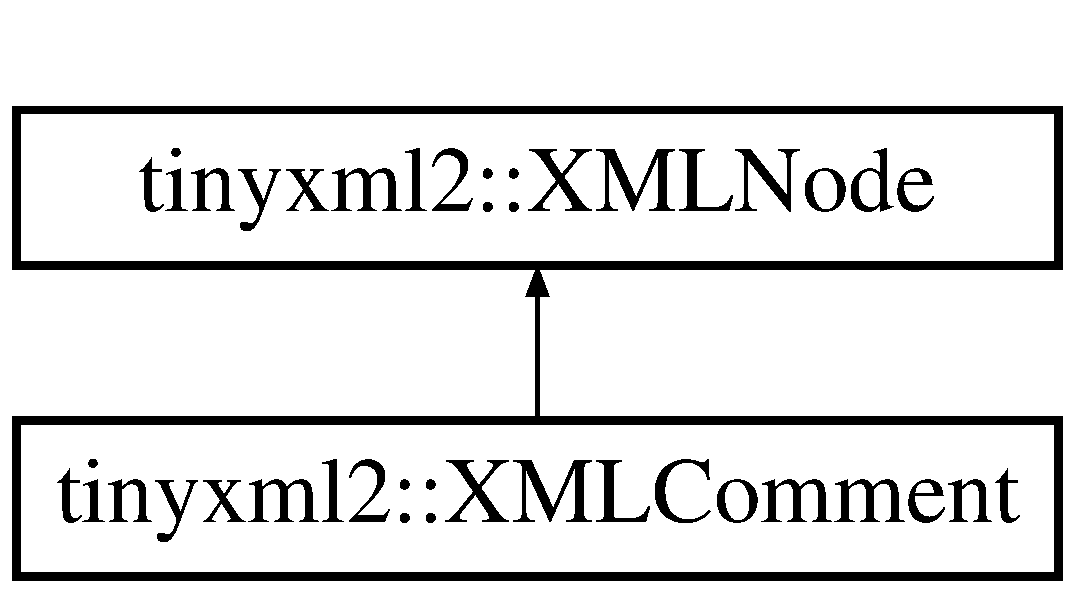
\includegraphics[height=2.000000cm]{classtinyxml2_1_1_x_m_l_comment}
\end{center}
\end{figure}
\subsection*{Public Member Functions}
\begin{DoxyCompactItemize}
\item 
virtual \hyperlink{classtinyxml2_1_1_x_m_l_comment}{X\-M\-L\-Comment} $\ast$ \hyperlink{classtinyxml2_1_1_x_m_l_comment_a8093e1dc8a34fa446d9dc3fde0e6c0ee}{To\-Comment} ()
\begin{DoxyCompactList}\small\item\em Safely cast to a Comment, or null. \end{DoxyCompactList}\item 
virtual const \hyperlink{classtinyxml2_1_1_x_m_l_comment}{X\-M\-L\-Comment} $\ast$ \hyperlink{classtinyxml2_1_1_x_m_l_comment_a422aabac22de7d9c9cad130897dd8b1c}{To\-Comment} () const 
\item 
virtual bool \hyperlink{classtinyxml2_1_1_x_m_l_comment_aa382b1be6a8b0650c16a2d88bb499335}{Accept} (\hyperlink{classtinyxml2_1_1_x_m_l_visitor}{X\-M\-L\-Visitor} $\ast$visitor) const 
\item 
char $\ast$ \hyperlink{classtinyxml2_1_1_x_m_l_comment_aa6ab35c3bb1c1840371dc32a2040c57f}{Parse\-Deep} (char $\ast$, \hyperlink{classtinyxml2_1_1_str_pair}{Str\-Pair} $\ast$end\-Tag)
\item 
virtual \hyperlink{classtinyxml2_1_1_x_m_l_node}{X\-M\-L\-Node} $\ast$ \hyperlink{classtinyxml2_1_1_x_m_l_comment_a90bb60193a691b484f5e1b487857016d}{Shallow\-Clone} (\hyperlink{classtinyxml2_1_1_x_m_l_document}{X\-M\-L\-Document} $\ast$document) const 
\item 
virtual bool \hyperlink{classtinyxml2_1_1_x_m_l_comment_a2d9f26757b0018fce933e74420cda22a}{Shallow\-Equal} (const \hyperlink{classtinyxml2_1_1_x_m_l_node}{X\-M\-L\-Node} $\ast$compare) const 
\end{DoxyCompactItemize}
\subsection*{Protected Member Functions}
\begin{DoxyCompactItemize}
\item 
\hyperlink{classtinyxml2_1_1_x_m_l_comment_ae6463adc3edd93a8e5a9b2b7e99cdf91}{X\-M\-L\-Comment} (\hyperlink{classtinyxml2_1_1_x_m_l_document}{X\-M\-L\-Document} $\ast$doc)
\item 
virtual \hyperlink{classtinyxml2_1_1_x_m_l_comment_ab592f69b47852455c1b32c5e31e453d0}{$\sim$\-X\-M\-L\-Comment} ()
\item 
\hyperlink{classtinyxml2_1_1_x_m_l_comment_aa0a9aae0850ac0e70d3cd20f6cb44447}{X\-M\-L\-Comment} (const \hyperlink{classtinyxml2_1_1_x_m_l_comment}{X\-M\-L\-Comment} \&)
\item 
\hyperlink{classtinyxml2_1_1_x_m_l_comment}{X\-M\-L\-Comment} \& \hyperlink{classtinyxml2_1_1_x_m_l_comment_ac8de55f8381d110740772e6bf6f5755a}{operator=} (const \hyperlink{classtinyxml2_1_1_x_m_l_comment}{X\-M\-L\-Comment} \&)
\end{DoxyCompactItemize}
\subsection*{Friends}
\begin{DoxyCompactItemize}
\item 
class \hyperlink{classtinyxml2_1_1_x_m_l_comment_a4eee3bda60c60a30e4e8cd4ea91c4c6e}{X\-M\-L\-Document}
\end{DoxyCompactItemize}
\subsection*{Additional Inherited Members}


\subsection{Detailed Description}
An \hyperlink{namespace_x_m_l}{X\-M\-L} Comment. 

Definition at line 878 of file tinyxml2.\-hpp.



\subsection{Constructor \& Destructor Documentation}
\hypertarget{classtinyxml2_1_1_x_m_l_comment_ae6463adc3edd93a8e5a9b2b7e99cdf91}{\index{tinyxml2\-::\-X\-M\-L\-Comment@{tinyxml2\-::\-X\-M\-L\-Comment}!X\-M\-L\-Comment@{X\-M\-L\-Comment}}
\index{X\-M\-L\-Comment@{X\-M\-L\-Comment}!tinyxml2::XMLComment@{tinyxml2\-::\-X\-M\-L\-Comment}}
\subsubsection[{X\-M\-L\-Comment}]{\setlength{\rightskip}{0pt plus 5cm}tinyxml2\-::\-X\-M\-L\-Comment\-::\-X\-M\-L\-Comment (
\begin{DoxyParamCaption}
\item[{{\bf X\-M\-L\-Document} $\ast$}]{doc}
\end{DoxyParamCaption}
)\hspace{0.3cm}{\ttfamily [protected]}}}\label{classtinyxml2_1_1_x_m_l_comment_ae6463adc3edd93a8e5a9b2b7e99cdf91}


Definition at line 905 of file tinyxml2.\-cpp.

\hypertarget{classtinyxml2_1_1_x_m_l_comment_ab592f69b47852455c1b32c5e31e453d0}{\index{tinyxml2\-::\-X\-M\-L\-Comment@{tinyxml2\-::\-X\-M\-L\-Comment}!$\sim$\-X\-M\-L\-Comment@{$\sim$\-X\-M\-L\-Comment}}
\index{$\sim$\-X\-M\-L\-Comment@{$\sim$\-X\-M\-L\-Comment}!tinyxml2::XMLComment@{tinyxml2\-::\-X\-M\-L\-Comment}}
\subsubsection[{$\sim$\-X\-M\-L\-Comment}]{\setlength{\rightskip}{0pt plus 5cm}tinyxml2\-::\-X\-M\-L\-Comment\-::$\sim$\-X\-M\-L\-Comment (
\begin{DoxyParamCaption}
{}
\end{DoxyParamCaption}
)\hspace{0.3cm}{\ttfamily [protected]}, {\ttfamily [virtual]}}}\label{classtinyxml2_1_1_x_m_l_comment_ab592f69b47852455c1b32c5e31e453d0}


Definition at line 910 of file tinyxml2.\-cpp.

\hypertarget{classtinyxml2_1_1_x_m_l_comment_aa0a9aae0850ac0e70d3cd20f6cb44447}{\index{tinyxml2\-::\-X\-M\-L\-Comment@{tinyxml2\-::\-X\-M\-L\-Comment}!X\-M\-L\-Comment@{X\-M\-L\-Comment}}
\index{X\-M\-L\-Comment@{X\-M\-L\-Comment}!tinyxml2::XMLComment@{tinyxml2\-::\-X\-M\-L\-Comment}}
\subsubsection[{X\-M\-L\-Comment}]{\setlength{\rightskip}{0pt plus 5cm}tinyxml2\-::\-X\-M\-L\-Comment\-::\-X\-M\-L\-Comment (
\begin{DoxyParamCaption}
\item[{const {\bf X\-M\-L\-Comment} \&}]{}
\end{DoxyParamCaption}
)\hspace{0.3cm}{\ttfamily [protected]}}}\label{classtinyxml2_1_1_x_m_l_comment_aa0a9aae0850ac0e70d3cd20f6cb44447}


\subsection{Member Function Documentation}
\hypertarget{classtinyxml2_1_1_x_m_l_comment_aa382b1be6a8b0650c16a2d88bb499335}{\index{tinyxml2\-::\-X\-M\-L\-Comment@{tinyxml2\-::\-X\-M\-L\-Comment}!Accept@{Accept}}
\index{Accept@{Accept}!tinyxml2::XMLComment@{tinyxml2\-::\-X\-M\-L\-Comment}}
\subsubsection[{Accept}]{\setlength{\rightskip}{0pt plus 5cm}bool tinyxml2\-::\-X\-M\-L\-Comment\-::\-Accept (
\begin{DoxyParamCaption}
\item[{{\bf X\-M\-L\-Visitor} $\ast$}]{visitor}
\end{DoxyParamCaption}
) const\hspace{0.3cm}{\ttfamily [virtual]}}}\label{classtinyxml2_1_1_x_m_l_comment_aa382b1be6a8b0650c16a2d88bb499335}
Accept a hierarchical visit of the nodes in the Tiny\-X\-M\-L-\/2 D\-O\-M. Every node in the \hyperlink{namespace_x_m_l}{X\-M\-L} tree will be conditionally visited and the host will be called back via the \hyperlink{classtinyxml2_1_1_x_m_l_visitor}{X\-M\-L\-Visitor} interface.

This is essentially a S\-A\-X interface for Tiny\-X\-M\-L-\/2. (Note however it doesn't re-\/parse the \hyperlink{namespace_x_m_l}{X\-M\-L} for the callbacks, so the performance of Tiny\-X\-M\-L-\/2 is unchanged by using this interface versus any other.)

The interface has been based on ideas from\-:


\begin{DoxyItemize}
\item \href{http://www.saxproject.org/}{\tt http\-://www.\-saxproject.\-org/}
\item \href{http://c2.com/cgi/wiki?HierarchicalVisitorPattern}{\tt http\-://c2.\-com/cgi/wiki?\-Hierarchical\-Visitor\-Pattern}
\end{DoxyItemize}

Which are both good references for \char`\"{}visiting\char`\"{}.

An example of using \hyperlink{classtinyxml2_1_1_x_m_l_comment_aa382b1be6a8b0650c16a2d88bb499335}{Accept()}\-: \begin{DoxyVerb}XMLPrinter printer;
tinyxmlDoc.Accept( &printer );
const char* xmlcstr = printer.CStr();
\end{DoxyVerb}
 

Implements \hyperlink{classtinyxml2_1_1_x_m_l_node_a81e66df0a44c67a7af17f3b77a152785}{tinyxml2\-::\-X\-M\-L\-Node}.



Definition at line 943 of file tinyxml2.\-cpp.

\hypertarget{classtinyxml2_1_1_x_m_l_comment_ac8de55f8381d110740772e6bf6f5755a}{\index{tinyxml2\-::\-X\-M\-L\-Comment@{tinyxml2\-::\-X\-M\-L\-Comment}!operator=@{operator=}}
\index{operator=@{operator=}!tinyxml2::XMLComment@{tinyxml2\-::\-X\-M\-L\-Comment}}
\subsubsection[{operator=}]{\setlength{\rightskip}{0pt plus 5cm}{\bf X\-M\-L\-Comment}\& tinyxml2\-::\-X\-M\-L\-Comment\-::operator= (
\begin{DoxyParamCaption}
\item[{const {\bf X\-M\-L\-Comment} \&}]{}
\end{DoxyParamCaption}
)\hspace{0.3cm}{\ttfamily [protected]}}}\label{classtinyxml2_1_1_x_m_l_comment_ac8de55f8381d110740772e6bf6f5755a}
\hypertarget{classtinyxml2_1_1_x_m_l_comment_aa6ab35c3bb1c1840371dc32a2040c57f}{\index{tinyxml2\-::\-X\-M\-L\-Comment@{tinyxml2\-::\-X\-M\-L\-Comment}!Parse\-Deep@{Parse\-Deep}}
\index{Parse\-Deep@{Parse\-Deep}!tinyxml2::XMLComment@{tinyxml2\-::\-X\-M\-L\-Comment}}
\subsubsection[{Parse\-Deep}]{\setlength{\rightskip}{0pt plus 5cm}char $\ast$ tinyxml2\-::\-X\-M\-L\-Comment\-::\-Parse\-Deep (
\begin{DoxyParamCaption}
\item[{char $\ast$}]{p, }
\item[{{\bf Str\-Pair} $\ast$}]{end\-Tag}
\end{DoxyParamCaption}
)\hspace{0.3cm}{\ttfamily [virtual]}}}\label{classtinyxml2_1_1_x_m_l_comment_aa6ab35c3bb1c1840371dc32a2040c57f}


Reimplemented from \hyperlink{classtinyxml2_1_1_x_m_l_node_a7610d0f603e8b603d2078521811a23c1}{tinyxml2\-::\-X\-M\-L\-Node}.



Definition at line 915 of file tinyxml2.\-cpp.

\hypertarget{classtinyxml2_1_1_x_m_l_comment_a90bb60193a691b484f5e1b487857016d}{\index{tinyxml2\-::\-X\-M\-L\-Comment@{tinyxml2\-::\-X\-M\-L\-Comment}!Shallow\-Clone@{Shallow\-Clone}}
\index{Shallow\-Clone@{Shallow\-Clone}!tinyxml2::XMLComment@{tinyxml2\-::\-X\-M\-L\-Comment}}
\subsubsection[{Shallow\-Clone}]{\setlength{\rightskip}{0pt plus 5cm}{\bf X\-M\-L\-Node} $\ast$ tinyxml2\-::\-X\-M\-L\-Comment\-::\-Shallow\-Clone (
\begin{DoxyParamCaption}
\item[{{\bf X\-M\-L\-Document} $\ast$}]{document}
\end{DoxyParamCaption}
) const\hspace{0.3cm}{\ttfamily [virtual]}}}\label{classtinyxml2_1_1_x_m_l_comment_a90bb60193a691b484f5e1b487857016d}
Make a copy of this node, but not its children. You may pass in a Document pointer that will be the owner of the new Node. If the 'document' is null, then the node returned will be allocated from the current Document. (this-\/$>$\hyperlink{classtinyxml2_1_1_x_m_l_node_af343d1ef0b45c0020e62d784d7e67a68}{Get\-Document()})

Note\-: if called on a \hyperlink{classtinyxml2_1_1_x_m_l_document}{X\-M\-L\-Document}, this will return null. 

Implements \hyperlink{classtinyxml2_1_1_x_m_l_node_a8402cbd3129d20e9e6024bbcc0531283}{tinyxml2\-::\-X\-M\-L\-Node}.



Definition at line 927 of file tinyxml2.\-cpp.

\hypertarget{classtinyxml2_1_1_x_m_l_comment_a2d9f26757b0018fce933e74420cda22a}{\index{tinyxml2\-::\-X\-M\-L\-Comment@{tinyxml2\-::\-X\-M\-L\-Comment}!Shallow\-Equal@{Shallow\-Equal}}
\index{Shallow\-Equal@{Shallow\-Equal}!tinyxml2::XMLComment@{tinyxml2\-::\-X\-M\-L\-Comment}}
\subsubsection[{Shallow\-Equal}]{\setlength{\rightskip}{0pt plus 5cm}bool tinyxml2\-::\-X\-M\-L\-Comment\-::\-Shallow\-Equal (
\begin{DoxyParamCaption}
\item[{const {\bf X\-M\-L\-Node} $\ast$}]{compare}
\end{DoxyParamCaption}
) const\hspace{0.3cm}{\ttfamily [virtual]}}}\label{classtinyxml2_1_1_x_m_l_comment_a2d9f26757b0018fce933e74420cda22a}
Test if 2 nodes are the same, but don't test children. The 2 nodes do not need to be in the same Document.

Note\-: if called on a \hyperlink{classtinyxml2_1_1_x_m_l_document}{X\-M\-L\-Document}, this will return false. 

Implements \hyperlink{classtinyxml2_1_1_x_m_l_node_a7ce18b751c3ea09eac292dca264f9226}{tinyxml2\-::\-X\-M\-L\-Node}.



Definition at line 937 of file tinyxml2.\-cpp.

\hypertarget{classtinyxml2_1_1_x_m_l_comment_a8093e1dc8a34fa446d9dc3fde0e6c0ee}{\index{tinyxml2\-::\-X\-M\-L\-Comment@{tinyxml2\-::\-X\-M\-L\-Comment}!To\-Comment@{To\-Comment}}
\index{To\-Comment@{To\-Comment}!tinyxml2::XMLComment@{tinyxml2\-::\-X\-M\-L\-Comment}}
\subsubsection[{To\-Comment}]{\setlength{\rightskip}{0pt plus 5cm}virtual {\bf X\-M\-L\-Comment}$\ast$ tinyxml2\-::\-X\-M\-L\-Comment\-::\-To\-Comment (
\begin{DoxyParamCaption}
{}
\end{DoxyParamCaption}
)\hspace{0.3cm}{\ttfamily [inline]}, {\ttfamily [virtual]}}}\label{classtinyxml2_1_1_x_m_l_comment_a8093e1dc8a34fa446d9dc3fde0e6c0ee}


Safely cast to a Comment, or null. 



Reimplemented from \hyperlink{classtinyxml2_1_1_x_m_l_node_aff47671055aa99840a1c1ebd661e63e3}{tinyxml2\-::\-X\-M\-L\-Node}.



Definition at line 882 of file tinyxml2.\-hpp.

\hypertarget{classtinyxml2_1_1_x_m_l_comment_a422aabac22de7d9c9cad130897dd8b1c}{\index{tinyxml2\-::\-X\-M\-L\-Comment@{tinyxml2\-::\-X\-M\-L\-Comment}!To\-Comment@{To\-Comment}}
\index{To\-Comment@{To\-Comment}!tinyxml2::XMLComment@{tinyxml2\-::\-X\-M\-L\-Comment}}
\subsubsection[{To\-Comment}]{\setlength{\rightskip}{0pt plus 5cm}virtual const {\bf X\-M\-L\-Comment}$\ast$ tinyxml2\-::\-X\-M\-L\-Comment\-::\-To\-Comment (
\begin{DoxyParamCaption}
{}
\end{DoxyParamCaption}
) const\hspace{0.3cm}{\ttfamily [inline]}, {\ttfamily [virtual]}}}\label{classtinyxml2_1_1_x_m_l_comment_a422aabac22de7d9c9cad130897dd8b1c}


Reimplemented from \hyperlink{classtinyxml2_1_1_x_m_l_node_a157ce3a00ea5ee5a85b7103138e85e8a}{tinyxml2\-::\-X\-M\-L\-Node}.



Definition at line 885 of file tinyxml2.\-hpp.



\subsection{Friends And Related Function Documentation}
\hypertarget{classtinyxml2_1_1_x_m_l_comment_a4eee3bda60c60a30e4e8cd4ea91c4c6e}{\index{tinyxml2\-::\-X\-M\-L\-Comment@{tinyxml2\-::\-X\-M\-L\-Comment}!X\-M\-L\-Document@{X\-M\-L\-Document}}
\index{X\-M\-L\-Document@{X\-M\-L\-Document}!tinyxml2::XMLComment@{tinyxml2\-::\-X\-M\-L\-Comment}}
\subsubsection[{X\-M\-L\-Document}]{\setlength{\rightskip}{0pt plus 5cm}friend class {\bf X\-M\-L\-Document}\hspace{0.3cm}{\ttfamily [friend]}}}\label{classtinyxml2_1_1_x_m_l_comment_a4eee3bda60c60a30e4e8cd4ea91c4c6e}


Definition at line 880 of file tinyxml2.\-hpp.



The documentation for this class was generated from the following files\-:\begin{DoxyCompactItemize}
\item 
Glide/\hyperlink{tinyxml2_8hpp}{tinyxml2.\-hpp}\item 
Glide/\hyperlink{tinyxml2_8cpp}{tinyxml2.\-cpp}\end{DoxyCompactItemize}

\hypertarget{classtinyxml2_1_1_x_m_l_const_handle}{\section{tinyxml2\-:\-:X\-M\-L\-Const\-Handle Class Reference}
\label{classtinyxml2_1_1_x_m_l_const_handle}\index{tinyxml2\-::\-X\-M\-L\-Const\-Handle@{tinyxml2\-::\-X\-M\-L\-Const\-Handle}}
}


{\ttfamily \#include $<$tinyxml2.\-hpp$>$}

\subsection*{Public Member Functions}
\begin{DoxyCompactItemize}
\item 
\hyperlink{classtinyxml2_1_1_x_m_l_const_handle_a098bda71fa11d7c74ccddab59d5dd534}{X\-M\-L\-Const\-Handle} (const \hyperlink{classtinyxml2_1_1_x_m_l_node}{X\-M\-L\-Node} $\ast$node)
\item 
\hyperlink{classtinyxml2_1_1_x_m_l_const_handle_a8420a0c4720637e0529e78c2e22f2b0b}{X\-M\-L\-Const\-Handle} (const \hyperlink{classtinyxml2_1_1_x_m_l_node}{X\-M\-L\-Node} \&node)
\item 
\hyperlink{classtinyxml2_1_1_x_m_l_const_handle_a639317ad315ff24f4ef0dc69312d7303}{X\-M\-L\-Const\-Handle} (const \hyperlink{classtinyxml2_1_1_x_m_l_const_handle}{X\-M\-L\-Const\-Handle} \&ref)
\item 
\hyperlink{classtinyxml2_1_1_x_m_l_const_handle}{X\-M\-L\-Const\-Handle} \& \hyperlink{classtinyxml2_1_1_x_m_l_const_handle_a2d74c91df1ff9aa5f9b57e3dceddbf94}{operator=} (const \hyperlink{classtinyxml2_1_1_x_m_l_const_handle}{X\-M\-L\-Const\-Handle} \&ref)
\item 
const \hyperlink{classtinyxml2_1_1_x_m_l_const_handle}{X\-M\-L\-Const\-Handle} \hyperlink{classtinyxml2_1_1_x_m_l_const_handle_a64c4ff7074effc1fd181d68d23f9d1e4}{First\-Child} () const 
\item 
const \hyperlink{classtinyxml2_1_1_x_m_l_const_handle}{X\-M\-L\-Const\-Handle} \hyperlink{classtinyxml2_1_1_x_m_l_const_handle_a5c197d0b57f8e560d93356a4a281469c}{First\-Child\-Element} (const char $\ast$value=0) const 
\item 
const \hyperlink{classtinyxml2_1_1_x_m_l_const_handle}{X\-M\-L\-Const\-Handle} \hyperlink{classtinyxml2_1_1_x_m_l_const_handle_afec9a68e7951193bc5a6e876d602f263}{Last\-Child} () const 
\item 
const \hyperlink{classtinyxml2_1_1_x_m_l_const_handle}{X\-M\-L\-Const\-Handle} \hyperlink{classtinyxml2_1_1_x_m_l_const_handle_a1c400e66dace6fdab4927adb21090059}{Last\-Child\-Element} (const char $\ast$\-\_\-value=0) const 
\item 
const \hyperlink{classtinyxml2_1_1_x_m_l_const_handle}{X\-M\-L\-Const\-Handle} \hyperlink{classtinyxml2_1_1_x_m_l_const_handle_a6917564e26b2c20ebdcb23c7940ad80a}{Previous\-Sibling} () const 
\item 
const \hyperlink{classtinyxml2_1_1_x_m_l_const_handle}{X\-M\-L\-Const\-Handle} \hyperlink{classtinyxml2_1_1_x_m_l_const_handle_acb2e1c5762eff9f6ed72d1a2dfc14271}{Previous\-Sibling\-Element} (const char $\ast$\-\_\-value=0) const 
\item 
const \hyperlink{classtinyxml2_1_1_x_m_l_const_handle}{X\-M\-L\-Const\-Handle} \hyperlink{classtinyxml2_1_1_x_m_l_const_handle_a596e248c8014d718f41658502a2e221b}{Next\-Sibling} () const 
\item 
const \hyperlink{classtinyxml2_1_1_x_m_l_const_handle}{X\-M\-L\-Const\-Handle} \hyperlink{classtinyxml2_1_1_x_m_l_const_handle_a3bbdd3d866c750473bd69a232704503b}{Next\-Sibling\-Element} (const char $\ast$\-\_\-value=0) const 
\item 
const \hyperlink{classtinyxml2_1_1_x_m_l_node}{X\-M\-L\-Node} $\ast$ \hyperlink{classtinyxml2_1_1_x_m_l_const_handle_a95d0256318c10c3f75fa5f8ffb3e4bc1}{To\-Node} () const 
\item 
const \hyperlink{classtinyxml2_1_1_x_m_l_element}{X\-M\-L\-Element} $\ast$ \hyperlink{classtinyxml2_1_1_x_m_l_const_handle_a5a48adefc2a5e70d4ce5b55692a0e2f9}{To\-Element} () const 
\item 
const \hyperlink{classtinyxml2_1_1_x_m_l_text}{X\-M\-L\-Text} $\ast$ \hyperlink{classtinyxml2_1_1_x_m_l_const_handle_ad86ca7dbb20d0495ae357fe7a866e0be}{To\-Text} () const 
\item 
const \hyperlink{classtinyxml2_1_1_x_m_l_unknown}{X\-M\-L\-Unknown} $\ast$ \hyperlink{classtinyxml2_1_1_x_m_l_const_handle_acb358a329e54fa204ed2d0b181566828}{To\-Unknown} () const 
\item 
const \hyperlink{classtinyxml2_1_1_x_m_l_declaration}{X\-M\-L\-Declaration} $\ast$ \hyperlink{classtinyxml2_1_1_x_m_l_const_handle_a5de0c175845bc30a6f9b3d88d8877eaf}{To\-Declaration} () const 
\end{DoxyCompactItemize}


\subsection{Detailed Description}
A variant of the \hyperlink{classtinyxml2_1_1_x_m_l_handle}{X\-M\-L\-Handle} class for working with const X\-M\-L\-Nodes and Documents. It is the same in all regards, except for the 'const' qualifiers. See \hyperlink{classtinyxml2_1_1_x_m_l_handle}{X\-M\-L\-Handle} for A\-P\-I. 

Definition at line 1770 of file tinyxml2.\-hpp.



\subsection{Constructor \& Destructor Documentation}
\hypertarget{classtinyxml2_1_1_x_m_l_const_handle_a098bda71fa11d7c74ccddab59d5dd534}{\index{tinyxml2\-::\-X\-M\-L\-Const\-Handle@{tinyxml2\-::\-X\-M\-L\-Const\-Handle}!X\-M\-L\-Const\-Handle@{X\-M\-L\-Const\-Handle}}
\index{X\-M\-L\-Const\-Handle@{X\-M\-L\-Const\-Handle}!tinyxml2::XMLConstHandle@{tinyxml2\-::\-X\-M\-L\-Const\-Handle}}
\subsubsection[{X\-M\-L\-Const\-Handle}]{\setlength{\rightskip}{0pt plus 5cm}tinyxml2\-::\-X\-M\-L\-Const\-Handle\-::\-X\-M\-L\-Const\-Handle (
\begin{DoxyParamCaption}
\item[{const {\bf X\-M\-L\-Node} $\ast$}]{node}
\end{DoxyParamCaption}
)\hspace{0.3cm}{\ttfamily [inline]}}}\label{classtinyxml2_1_1_x_m_l_const_handle_a098bda71fa11d7c74ccddab59d5dd534}


Definition at line 1773 of file tinyxml2.\-hpp.

\hypertarget{classtinyxml2_1_1_x_m_l_const_handle_a8420a0c4720637e0529e78c2e22f2b0b}{\index{tinyxml2\-::\-X\-M\-L\-Const\-Handle@{tinyxml2\-::\-X\-M\-L\-Const\-Handle}!X\-M\-L\-Const\-Handle@{X\-M\-L\-Const\-Handle}}
\index{X\-M\-L\-Const\-Handle@{X\-M\-L\-Const\-Handle}!tinyxml2::XMLConstHandle@{tinyxml2\-::\-X\-M\-L\-Const\-Handle}}
\subsubsection[{X\-M\-L\-Const\-Handle}]{\setlength{\rightskip}{0pt plus 5cm}tinyxml2\-::\-X\-M\-L\-Const\-Handle\-::\-X\-M\-L\-Const\-Handle (
\begin{DoxyParamCaption}
\item[{const {\bf X\-M\-L\-Node} \&}]{node}
\end{DoxyParamCaption}
)\hspace{0.3cm}{\ttfamily [inline]}}}\label{classtinyxml2_1_1_x_m_l_const_handle_a8420a0c4720637e0529e78c2e22f2b0b}


Definition at line 1776 of file tinyxml2.\-hpp.

\hypertarget{classtinyxml2_1_1_x_m_l_const_handle_a639317ad315ff24f4ef0dc69312d7303}{\index{tinyxml2\-::\-X\-M\-L\-Const\-Handle@{tinyxml2\-::\-X\-M\-L\-Const\-Handle}!X\-M\-L\-Const\-Handle@{X\-M\-L\-Const\-Handle}}
\index{X\-M\-L\-Const\-Handle@{X\-M\-L\-Const\-Handle}!tinyxml2::XMLConstHandle@{tinyxml2\-::\-X\-M\-L\-Const\-Handle}}
\subsubsection[{X\-M\-L\-Const\-Handle}]{\setlength{\rightskip}{0pt plus 5cm}tinyxml2\-::\-X\-M\-L\-Const\-Handle\-::\-X\-M\-L\-Const\-Handle (
\begin{DoxyParamCaption}
\item[{const {\bf X\-M\-L\-Const\-Handle} \&}]{ref}
\end{DoxyParamCaption}
)\hspace{0.3cm}{\ttfamily [inline]}}}\label{classtinyxml2_1_1_x_m_l_const_handle_a639317ad315ff24f4ef0dc69312d7303}


Definition at line 1779 of file tinyxml2.\-hpp.



\subsection{Member Function Documentation}
\hypertarget{classtinyxml2_1_1_x_m_l_const_handle_a64c4ff7074effc1fd181d68d23f9d1e4}{\index{tinyxml2\-::\-X\-M\-L\-Const\-Handle@{tinyxml2\-::\-X\-M\-L\-Const\-Handle}!First\-Child@{First\-Child}}
\index{First\-Child@{First\-Child}!tinyxml2::XMLConstHandle@{tinyxml2\-::\-X\-M\-L\-Const\-Handle}}
\subsubsection[{First\-Child}]{\setlength{\rightskip}{0pt plus 5cm}const {\bf X\-M\-L\-Const\-Handle} tinyxml2\-::\-X\-M\-L\-Const\-Handle\-::\-First\-Child (
\begin{DoxyParamCaption}
{}
\end{DoxyParamCaption}
) const\hspace{0.3cm}{\ttfamily [inline]}}}\label{classtinyxml2_1_1_x_m_l_const_handle_a64c4ff7074effc1fd181d68d23f9d1e4}


Definition at line 1788 of file tinyxml2.\-hpp.

\hypertarget{classtinyxml2_1_1_x_m_l_const_handle_a5c197d0b57f8e560d93356a4a281469c}{\index{tinyxml2\-::\-X\-M\-L\-Const\-Handle@{tinyxml2\-::\-X\-M\-L\-Const\-Handle}!First\-Child\-Element@{First\-Child\-Element}}
\index{First\-Child\-Element@{First\-Child\-Element}!tinyxml2::XMLConstHandle@{tinyxml2\-::\-X\-M\-L\-Const\-Handle}}
\subsubsection[{First\-Child\-Element}]{\setlength{\rightskip}{0pt plus 5cm}const {\bf X\-M\-L\-Const\-Handle} tinyxml2\-::\-X\-M\-L\-Const\-Handle\-::\-First\-Child\-Element (
\begin{DoxyParamCaption}
\item[{const char $\ast$}]{value = {\ttfamily 0}}
\end{DoxyParamCaption}
) const\hspace{0.3cm}{\ttfamily [inline]}}}\label{classtinyxml2_1_1_x_m_l_const_handle_a5c197d0b57f8e560d93356a4a281469c}


Definition at line 1791 of file tinyxml2.\-hpp.

\hypertarget{classtinyxml2_1_1_x_m_l_const_handle_afec9a68e7951193bc5a6e876d602f263}{\index{tinyxml2\-::\-X\-M\-L\-Const\-Handle@{tinyxml2\-::\-X\-M\-L\-Const\-Handle}!Last\-Child@{Last\-Child}}
\index{Last\-Child@{Last\-Child}!tinyxml2::XMLConstHandle@{tinyxml2\-::\-X\-M\-L\-Const\-Handle}}
\subsubsection[{Last\-Child}]{\setlength{\rightskip}{0pt plus 5cm}const {\bf X\-M\-L\-Const\-Handle} tinyxml2\-::\-X\-M\-L\-Const\-Handle\-::\-Last\-Child (
\begin{DoxyParamCaption}
{}
\end{DoxyParamCaption}
) const\hspace{0.3cm}{\ttfamily [inline]}}}\label{classtinyxml2_1_1_x_m_l_const_handle_afec9a68e7951193bc5a6e876d602f263}


Definition at line 1794 of file tinyxml2.\-hpp.

\hypertarget{classtinyxml2_1_1_x_m_l_const_handle_a1c400e66dace6fdab4927adb21090059}{\index{tinyxml2\-::\-X\-M\-L\-Const\-Handle@{tinyxml2\-::\-X\-M\-L\-Const\-Handle}!Last\-Child\-Element@{Last\-Child\-Element}}
\index{Last\-Child\-Element@{Last\-Child\-Element}!tinyxml2::XMLConstHandle@{tinyxml2\-::\-X\-M\-L\-Const\-Handle}}
\subsubsection[{Last\-Child\-Element}]{\setlength{\rightskip}{0pt plus 5cm}const {\bf X\-M\-L\-Const\-Handle} tinyxml2\-::\-X\-M\-L\-Const\-Handle\-::\-Last\-Child\-Element (
\begin{DoxyParamCaption}
\item[{const char $\ast$}]{\-\_\-value = {\ttfamily 0}}
\end{DoxyParamCaption}
) const\hspace{0.3cm}{\ttfamily [inline]}}}\label{classtinyxml2_1_1_x_m_l_const_handle_a1c400e66dace6fdab4927adb21090059}


Definition at line 1797 of file tinyxml2.\-hpp.

\hypertarget{classtinyxml2_1_1_x_m_l_const_handle_a596e248c8014d718f41658502a2e221b}{\index{tinyxml2\-::\-X\-M\-L\-Const\-Handle@{tinyxml2\-::\-X\-M\-L\-Const\-Handle}!Next\-Sibling@{Next\-Sibling}}
\index{Next\-Sibling@{Next\-Sibling}!tinyxml2::XMLConstHandle@{tinyxml2\-::\-X\-M\-L\-Const\-Handle}}
\subsubsection[{Next\-Sibling}]{\setlength{\rightskip}{0pt plus 5cm}const {\bf X\-M\-L\-Const\-Handle} tinyxml2\-::\-X\-M\-L\-Const\-Handle\-::\-Next\-Sibling (
\begin{DoxyParamCaption}
{}
\end{DoxyParamCaption}
) const\hspace{0.3cm}{\ttfamily [inline]}}}\label{classtinyxml2_1_1_x_m_l_const_handle_a596e248c8014d718f41658502a2e221b}


Definition at line 1806 of file tinyxml2.\-hpp.

\hypertarget{classtinyxml2_1_1_x_m_l_const_handle_a3bbdd3d866c750473bd69a232704503b}{\index{tinyxml2\-::\-X\-M\-L\-Const\-Handle@{tinyxml2\-::\-X\-M\-L\-Const\-Handle}!Next\-Sibling\-Element@{Next\-Sibling\-Element}}
\index{Next\-Sibling\-Element@{Next\-Sibling\-Element}!tinyxml2::XMLConstHandle@{tinyxml2\-::\-X\-M\-L\-Const\-Handle}}
\subsubsection[{Next\-Sibling\-Element}]{\setlength{\rightskip}{0pt plus 5cm}const {\bf X\-M\-L\-Const\-Handle} tinyxml2\-::\-X\-M\-L\-Const\-Handle\-::\-Next\-Sibling\-Element (
\begin{DoxyParamCaption}
\item[{const char $\ast$}]{\-\_\-value = {\ttfamily 0}}
\end{DoxyParamCaption}
) const\hspace{0.3cm}{\ttfamily [inline]}}}\label{classtinyxml2_1_1_x_m_l_const_handle_a3bbdd3d866c750473bd69a232704503b}


Definition at line 1809 of file tinyxml2.\-hpp.

\hypertarget{classtinyxml2_1_1_x_m_l_const_handle_a2d74c91df1ff9aa5f9b57e3dceddbf94}{\index{tinyxml2\-::\-X\-M\-L\-Const\-Handle@{tinyxml2\-::\-X\-M\-L\-Const\-Handle}!operator=@{operator=}}
\index{operator=@{operator=}!tinyxml2::XMLConstHandle@{tinyxml2\-::\-X\-M\-L\-Const\-Handle}}
\subsubsection[{operator=}]{\setlength{\rightskip}{0pt plus 5cm}{\bf X\-M\-L\-Const\-Handle}\& tinyxml2\-::\-X\-M\-L\-Const\-Handle\-::operator= (
\begin{DoxyParamCaption}
\item[{const {\bf X\-M\-L\-Const\-Handle} \&}]{ref}
\end{DoxyParamCaption}
)\hspace{0.3cm}{\ttfamily [inline]}}}\label{classtinyxml2_1_1_x_m_l_const_handle_a2d74c91df1ff9aa5f9b57e3dceddbf94}


Definition at line 1783 of file tinyxml2.\-hpp.

\hypertarget{classtinyxml2_1_1_x_m_l_const_handle_a6917564e26b2c20ebdcb23c7940ad80a}{\index{tinyxml2\-::\-X\-M\-L\-Const\-Handle@{tinyxml2\-::\-X\-M\-L\-Const\-Handle}!Previous\-Sibling@{Previous\-Sibling}}
\index{Previous\-Sibling@{Previous\-Sibling}!tinyxml2::XMLConstHandle@{tinyxml2\-::\-X\-M\-L\-Const\-Handle}}
\subsubsection[{Previous\-Sibling}]{\setlength{\rightskip}{0pt plus 5cm}const {\bf X\-M\-L\-Const\-Handle} tinyxml2\-::\-X\-M\-L\-Const\-Handle\-::\-Previous\-Sibling (
\begin{DoxyParamCaption}
{}
\end{DoxyParamCaption}
) const\hspace{0.3cm}{\ttfamily [inline]}}}\label{classtinyxml2_1_1_x_m_l_const_handle_a6917564e26b2c20ebdcb23c7940ad80a}


Definition at line 1800 of file tinyxml2.\-hpp.

\hypertarget{classtinyxml2_1_1_x_m_l_const_handle_acb2e1c5762eff9f6ed72d1a2dfc14271}{\index{tinyxml2\-::\-X\-M\-L\-Const\-Handle@{tinyxml2\-::\-X\-M\-L\-Const\-Handle}!Previous\-Sibling\-Element@{Previous\-Sibling\-Element}}
\index{Previous\-Sibling\-Element@{Previous\-Sibling\-Element}!tinyxml2::XMLConstHandle@{tinyxml2\-::\-X\-M\-L\-Const\-Handle}}
\subsubsection[{Previous\-Sibling\-Element}]{\setlength{\rightskip}{0pt plus 5cm}const {\bf X\-M\-L\-Const\-Handle} tinyxml2\-::\-X\-M\-L\-Const\-Handle\-::\-Previous\-Sibling\-Element (
\begin{DoxyParamCaption}
\item[{const char $\ast$}]{\-\_\-value = {\ttfamily 0}}
\end{DoxyParamCaption}
) const\hspace{0.3cm}{\ttfamily [inline]}}}\label{classtinyxml2_1_1_x_m_l_const_handle_acb2e1c5762eff9f6ed72d1a2dfc14271}


Definition at line 1803 of file tinyxml2.\-hpp.

\hypertarget{classtinyxml2_1_1_x_m_l_const_handle_a5de0c175845bc30a6f9b3d88d8877eaf}{\index{tinyxml2\-::\-X\-M\-L\-Const\-Handle@{tinyxml2\-::\-X\-M\-L\-Const\-Handle}!To\-Declaration@{To\-Declaration}}
\index{To\-Declaration@{To\-Declaration}!tinyxml2::XMLConstHandle@{tinyxml2\-::\-X\-M\-L\-Const\-Handle}}
\subsubsection[{To\-Declaration}]{\setlength{\rightskip}{0pt plus 5cm}const {\bf X\-M\-L\-Declaration}$\ast$ tinyxml2\-::\-X\-M\-L\-Const\-Handle\-::\-To\-Declaration (
\begin{DoxyParamCaption}
{}
\end{DoxyParamCaption}
) const\hspace{0.3cm}{\ttfamily [inline]}}}\label{classtinyxml2_1_1_x_m_l_const_handle_a5de0c175845bc30a6f9b3d88d8877eaf}


Definition at line 1826 of file tinyxml2.\-hpp.

\hypertarget{classtinyxml2_1_1_x_m_l_const_handle_a5a48adefc2a5e70d4ce5b55692a0e2f9}{\index{tinyxml2\-::\-X\-M\-L\-Const\-Handle@{tinyxml2\-::\-X\-M\-L\-Const\-Handle}!To\-Element@{To\-Element}}
\index{To\-Element@{To\-Element}!tinyxml2::XMLConstHandle@{tinyxml2\-::\-X\-M\-L\-Const\-Handle}}
\subsubsection[{To\-Element}]{\setlength{\rightskip}{0pt plus 5cm}const {\bf X\-M\-L\-Element}$\ast$ tinyxml2\-::\-X\-M\-L\-Const\-Handle\-::\-To\-Element (
\begin{DoxyParamCaption}
{}
\end{DoxyParamCaption}
) const\hspace{0.3cm}{\ttfamily [inline]}}}\label{classtinyxml2_1_1_x_m_l_const_handle_a5a48adefc2a5e70d4ce5b55692a0e2f9}


Definition at line 1817 of file tinyxml2.\-hpp.

\hypertarget{classtinyxml2_1_1_x_m_l_const_handle_a95d0256318c10c3f75fa5f8ffb3e4bc1}{\index{tinyxml2\-::\-X\-M\-L\-Const\-Handle@{tinyxml2\-::\-X\-M\-L\-Const\-Handle}!To\-Node@{To\-Node}}
\index{To\-Node@{To\-Node}!tinyxml2::XMLConstHandle@{tinyxml2\-::\-X\-M\-L\-Const\-Handle}}
\subsubsection[{To\-Node}]{\setlength{\rightskip}{0pt plus 5cm}const {\bf X\-M\-L\-Node}$\ast$ tinyxml2\-::\-X\-M\-L\-Const\-Handle\-::\-To\-Node (
\begin{DoxyParamCaption}
{}
\end{DoxyParamCaption}
) const\hspace{0.3cm}{\ttfamily [inline]}}}\label{classtinyxml2_1_1_x_m_l_const_handle_a95d0256318c10c3f75fa5f8ffb3e4bc1}


Definition at line 1814 of file tinyxml2.\-hpp.

\hypertarget{classtinyxml2_1_1_x_m_l_const_handle_ad86ca7dbb20d0495ae357fe7a866e0be}{\index{tinyxml2\-::\-X\-M\-L\-Const\-Handle@{tinyxml2\-::\-X\-M\-L\-Const\-Handle}!To\-Text@{To\-Text}}
\index{To\-Text@{To\-Text}!tinyxml2::XMLConstHandle@{tinyxml2\-::\-X\-M\-L\-Const\-Handle}}
\subsubsection[{To\-Text}]{\setlength{\rightskip}{0pt plus 5cm}const {\bf X\-M\-L\-Text}$\ast$ tinyxml2\-::\-X\-M\-L\-Const\-Handle\-::\-To\-Text (
\begin{DoxyParamCaption}
{}
\end{DoxyParamCaption}
) const\hspace{0.3cm}{\ttfamily [inline]}}}\label{classtinyxml2_1_1_x_m_l_const_handle_ad86ca7dbb20d0495ae357fe7a866e0be}


Definition at line 1820 of file tinyxml2.\-hpp.

\hypertarget{classtinyxml2_1_1_x_m_l_const_handle_acb358a329e54fa204ed2d0b181566828}{\index{tinyxml2\-::\-X\-M\-L\-Const\-Handle@{tinyxml2\-::\-X\-M\-L\-Const\-Handle}!To\-Unknown@{To\-Unknown}}
\index{To\-Unknown@{To\-Unknown}!tinyxml2::XMLConstHandle@{tinyxml2\-::\-X\-M\-L\-Const\-Handle}}
\subsubsection[{To\-Unknown}]{\setlength{\rightskip}{0pt plus 5cm}const {\bf X\-M\-L\-Unknown}$\ast$ tinyxml2\-::\-X\-M\-L\-Const\-Handle\-::\-To\-Unknown (
\begin{DoxyParamCaption}
{}
\end{DoxyParamCaption}
) const\hspace{0.3cm}{\ttfamily [inline]}}}\label{classtinyxml2_1_1_x_m_l_const_handle_acb358a329e54fa204ed2d0b181566828}


Definition at line 1823 of file tinyxml2.\-hpp.



The documentation for this class was generated from the following file\-:\begin{DoxyCompactItemize}
\item 
Glide/\hyperlink{tinyxml2_8hpp}{tinyxml2.\-hpp}\end{DoxyCompactItemize}

\hypertarget{classtinyxml2_1_1_x_m_l_declaration}{\section{tinyxml2\-:\-:X\-M\-L\-Declaration Class Reference}
\label{classtinyxml2_1_1_x_m_l_declaration}\index{tinyxml2\-::\-X\-M\-L\-Declaration@{tinyxml2\-::\-X\-M\-L\-Declaration}}
}


{\ttfamily \#include $<$tinyxml2.\-hpp$>$}

Inheritance diagram for tinyxml2\-:\-:X\-M\-L\-Declaration\-:\begin{figure}[H]
\begin{center}
\leavevmode
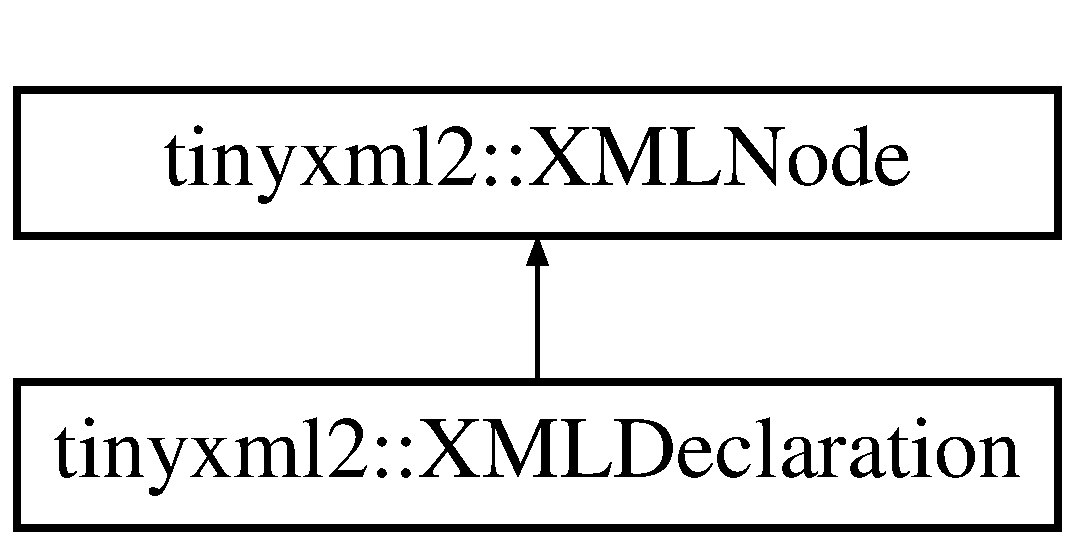
\includegraphics[height=2.000000cm]{classtinyxml2_1_1_x_m_l_declaration}
\end{center}
\end{figure}
\subsection*{Public Member Functions}
\begin{DoxyCompactItemize}
\item 
virtual \hyperlink{classtinyxml2_1_1_x_m_l_declaration}{X\-M\-L\-Declaration} $\ast$ \hyperlink{classtinyxml2_1_1_x_m_l_declaration_a159d8ac45865215e88059ea1e5b52fc5}{To\-Declaration} ()
\begin{DoxyCompactList}\small\item\em Safely cast to a Declaration, or null. \end{DoxyCompactList}\item 
virtual const \hyperlink{classtinyxml2_1_1_x_m_l_declaration}{X\-M\-L\-Declaration} $\ast$ \hyperlink{classtinyxml2_1_1_x_m_l_declaration_af724607a5fa810496fd6a21f5975a643}{To\-Declaration} () const 
\item 
virtual bool \hyperlink{classtinyxml2_1_1_x_m_l_declaration_a953a7359cc312d15218eb5843a4ca108}{Accept} (\hyperlink{classtinyxml2_1_1_x_m_l_visitor}{X\-M\-L\-Visitor} $\ast$visitor) const 
\item 
char $\ast$ \hyperlink{classtinyxml2_1_1_x_m_l_declaration_a19e33e0a9f9500f449261558c36f9a44}{Parse\-Deep} (char $\ast$, \hyperlink{classtinyxml2_1_1_str_pair}{Str\-Pair} $\ast$end\-Tag)
\item 
virtual \hyperlink{classtinyxml2_1_1_x_m_l_node}{X\-M\-L\-Node} $\ast$ \hyperlink{classtinyxml2_1_1_x_m_l_declaration_a39458732ee6796cfc85dd35d3c488e0b}{Shallow\-Clone} (\hyperlink{classtinyxml2_1_1_x_m_l_document}{X\-M\-L\-Document} $\ast$document) const 
\item 
virtual bool \hyperlink{classtinyxml2_1_1_x_m_l_declaration_ace0d2d9bc1b63278bd5e984ebe0c7bd0}{Shallow\-Equal} (const \hyperlink{classtinyxml2_1_1_x_m_l_node}{X\-M\-L\-Node} $\ast$compare) const 
\end{DoxyCompactItemize}
\subsection*{Protected Member Functions}
\begin{DoxyCompactItemize}
\item 
\hyperlink{classtinyxml2_1_1_x_m_l_declaration_aef9586f2ce5df5feba74dde49a242b06}{X\-M\-L\-Declaration} (\hyperlink{classtinyxml2_1_1_x_m_l_document}{X\-M\-L\-Document} $\ast$doc)
\item 
virtual \hyperlink{classtinyxml2_1_1_x_m_l_declaration_ab93d5bf4f5d58b4144963cf739cf6dcc}{$\sim$\-X\-M\-L\-Declaration} ()
\item 
\hyperlink{classtinyxml2_1_1_x_m_l_declaration_a5229cc0b31f034f93289af27ec3e2836}{X\-M\-L\-Declaration} (const \hyperlink{classtinyxml2_1_1_x_m_l_declaration}{X\-M\-L\-Declaration} \&)
\item 
\hyperlink{classtinyxml2_1_1_x_m_l_declaration}{X\-M\-L\-Declaration} \& \hyperlink{classtinyxml2_1_1_x_m_l_declaration_a79eb518c2c2b1b99a122a5d5a308b7ee}{operator=} (const \hyperlink{classtinyxml2_1_1_x_m_l_declaration}{X\-M\-L\-Declaration} \&)
\end{DoxyCompactItemize}
\subsection*{Friends}
\begin{DoxyCompactItemize}
\item 
class \hyperlink{classtinyxml2_1_1_x_m_l_declaration_a4eee3bda60c60a30e4e8cd4ea91c4c6e}{X\-M\-L\-Document}
\end{DoxyCompactItemize}
\subsection*{Additional Inherited Members}


\subsection{Detailed Description}
In correct \hyperlink{namespace_x_m_l}{X\-M\-L} the declaration is the first entry in the file. \begin{DoxyVerb}    <?xml version="1.0" standalone="yes"?>
\end{DoxyVerb}


Tiny\-X\-M\-L-\/2 will happily read or write files without a declaration, however.

The text of the declaration isn't interpreted. It is parsed and written as a string. 

Definition at line 916 of file tinyxml2.\-hpp.



\subsection{Constructor \& Destructor Documentation}
\hypertarget{classtinyxml2_1_1_x_m_l_declaration_aef9586f2ce5df5feba74dde49a242b06}{\index{tinyxml2\-::\-X\-M\-L\-Declaration@{tinyxml2\-::\-X\-M\-L\-Declaration}!X\-M\-L\-Declaration@{X\-M\-L\-Declaration}}
\index{X\-M\-L\-Declaration@{X\-M\-L\-Declaration}!tinyxml2::XMLDeclaration@{tinyxml2\-::\-X\-M\-L\-Declaration}}
\subsubsection[{X\-M\-L\-Declaration}]{\setlength{\rightskip}{0pt plus 5cm}tinyxml2\-::\-X\-M\-L\-Declaration\-::\-X\-M\-L\-Declaration (
\begin{DoxyParamCaption}
\item[{{\bf X\-M\-L\-Document} $\ast$}]{doc}
\end{DoxyParamCaption}
)\hspace{0.3cm}{\ttfamily [protected]}}}\label{classtinyxml2_1_1_x_m_l_declaration_aef9586f2ce5df5feba74dde49a242b06}


Definition at line 951 of file tinyxml2.\-cpp.

\hypertarget{classtinyxml2_1_1_x_m_l_declaration_ab93d5bf4f5d58b4144963cf739cf6dcc}{\index{tinyxml2\-::\-X\-M\-L\-Declaration@{tinyxml2\-::\-X\-M\-L\-Declaration}!$\sim$\-X\-M\-L\-Declaration@{$\sim$\-X\-M\-L\-Declaration}}
\index{$\sim$\-X\-M\-L\-Declaration@{$\sim$\-X\-M\-L\-Declaration}!tinyxml2::XMLDeclaration@{tinyxml2\-::\-X\-M\-L\-Declaration}}
\subsubsection[{$\sim$\-X\-M\-L\-Declaration}]{\setlength{\rightskip}{0pt plus 5cm}tinyxml2\-::\-X\-M\-L\-Declaration\-::$\sim$\-X\-M\-L\-Declaration (
\begin{DoxyParamCaption}
{}
\end{DoxyParamCaption}
)\hspace{0.3cm}{\ttfamily [protected]}, {\ttfamily [virtual]}}}\label{classtinyxml2_1_1_x_m_l_declaration_ab93d5bf4f5d58b4144963cf739cf6dcc}


Definition at line 956 of file tinyxml2.\-cpp.

\hypertarget{classtinyxml2_1_1_x_m_l_declaration_a5229cc0b31f034f93289af27ec3e2836}{\index{tinyxml2\-::\-X\-M\-L\-Declaration@{tinyxml2\-::\-X\-M\-L\-Declaration}!X\-M\-L\-Declaration@{X\-M\-L\-Declaration}}
\index{X\-M\-L\-Declaration@{X\-M\-L\-Declaration}!tinyxml2::XMLDeclaration@{tinyxml2\-::\-X\-M\-L\-Declaration}}
\subsubsection[{X\-M\-L\-Declaration}]{\setlength{\rightskip}{0pt plus 5cm}tinyxml2\-::\-X\-M\-L\-Declaration\-::\-X\-M\-L\-Declaration (
\begin{DoxyParamCaption}
\item[{const {\bf X\-M\-L\-Declaration} \&}]{}
\end{DoxyParamCaption}
)\hspace{0.3cm}{\ttfamily [protected]}}}\label{classtinyxml2_1_1_x_m_l_declaration_a5229cc0b31f034f93289af27ec3e2836}


\subsection{Member Function Documentation}
\hypertarget{classtinyxml2_1_1_x_m_l_declaration_a953a7359cc312d15218eb5843a4ca108}{\index{tinyxml2\-::\-X\-M\-L\-Declaration@{tinyxml2\-::\-X\-M\-L\-Declaration}!Accept@{Accept}}
\index{Accept@{Accept}!tinyxml2::XMLDeclaration@{tinyxml2\-::\-X\-M\-L\-Declaration}}
\subsubsection[{Accept}]{\setlength{\rightskip}{0pt plus 5cm}bool tinyxml2\-::\-X\-M\-L\-Declaration\-::\-Accept (
\begin{DoxyParamCaption}
\item[{{\bf X\-M\-L\-Visitor} $\ast$}]{visitor}
\end{DoxyParamCaption}
) const\hspace{0.3cm}{\ttfamily [virtual]}}}\label{classtinyxml2_1_1_x_m_l_declaration_a953a7359cc312d15218eb5843a4ca108}
Accept a hierarchical visit of the nodes in the Tiny\-X\-M\-L-\/2 D\-O\-M. Every node in the \hyperlink{namespace_x_m_l}{X\-M\-L} tree will be conditionally visited and the host will be called back via the \hyperlink{classtinyxml2_1_1_x_m_l_visitor}{X\-M\-L\-Visitor} interface.

This is essentially a S\-A\-X interface for Tiny\-X\-M\-L-\/2. (Note however it doesn't re-\/parse the \hyperlink{namespace_x_m_l}{X\-M\-L} for the callbacks, so the performance of Tiny\-X\-M\-L-\/2 is unchanged by using this interface versus any other.)

The interface has been based on ideas from\-:


\begin{DoxyItemize}
\item \href{http://www.saxproject.org/}{\tt http\-://www.\-saxproject.\-org/}
\item \href{http://c2.com/cgi/wiki?HierarchicalVisitorPattern}{\tt http\-://c2.\-com/cgi/wiki?\-Hierarchical\-Visitor\-Pattern}
\end{DoxyItemize}

Which are both good references for \char`\"{}visiting\char`\"{}.

An example of using \hyperlink{classtinyxml2_1_1_x_m_l_declaration_a953a7359cc312d15218eb5843a4ca108}{Accept()}\-: \begin{DoxyVerb}XMLPrinter printer;
tinyxmlDoc.Accept( &printer );
const char* xmlcstr = printer.CStr();
\end{DoxyVerb}
 

Implements \hyperlink{classtinyxml2_1_1_x_m_l_node_a81e66df0a44c67a7af17f3b77a152785}{tinyxml2\-::\-X\-M\-L\-Node}.



Definition at line 991 of file tinyxml2.\-cpp.

\hypertarget{classtinyxml2_1_1_x_m_l_declaration_a79eb518c2c2b1b99a122a5d5a308b7ee}{\index{tinyxml2\-::\-X\-M\-L\-Declaration@{tinyxml2\-::\-X\-M\-L\-Declaration}!operator=@{operator=}}
\index{operator=@{operator=}!tinyxml2::XMLDeclaration@{tinyxml2\-::\-X\-M\-L\-Declaration}}
\subsubsection[{operator=}]{\setlength{\rightskip}{0pt plus 5cm}{\bf X\-M\-L\-Declaration}\& tinyxml2\-::\-X\-M\-L\-Declaration\-::operator= (
\begin{DoxyParamCaption}
\item[{const {\bf X\-M\-L\-Declaration} \&}]{}
\end{DoxyParamCaption}
)\hspace{0.3cm}{\ttfamily [protected]}}}\label{classtinyxml2_1_1_x_m_l_declaration_a79eb518c2c2b1b99a122a5d5a308b7ee}
\hypertarget{classtinyxml2_1_1_x_m_l_declaration_a19e33e0a9f9500f449261558c36f9a44}{\index{tinyxml2\-::\-X\-M\-L\-Declaration@{tinyxml2\-::\-X\-M\-L\-Declaration}!Parse\-Deep@{Parse\-Deep}}
\index{Parse\-Deep@{Parse\-Deep}!tinyxml2::XMLDeclaration@{tinyxml2\-::\-X\-M\-L\-Declaration}}
\subsubsection[{Parse\-Deep}]{\setlength{\rightskip}{0pt plus 5cm}char $\ast$ tinyxml2\-::\-X\-M\-L\-Declaration\-::\-Parse\-Deep (
\begin{DoxyParamCaption}
\item[{char $\ast$}]{p, }
\item[{{\bf Str\-Pair} $\ast$}]{end\-Tag}
\end{DoxyParamCaption}
)\hspace{0.3cm}{\ttfamily [virtual]}}}\label{classtinyxml2_1_1_x_m_l_declaration_a19e33e0a9f9500f449261558c36f9a44}


Reimplemented from \hyperlink{classtinyxml2_1_1_x_m_l_node_a7610d0f603e8b603d2078521811a23c1}{tinyxml2\-::\-X\-M\-L\-Node}.



Definition at line 962 of file tinyxml2.\-cpp.

\hypertarget{classtinyxml2_1_1_x_m_l_declaration_a39458732ee6796cfc85dd35d3c488e0b}{\index{tinyxml2\-::\-X\-M\-L\-Declaration@{tinyxml2\-::\-X\-M\-L\-Declaration}!Shallow\-Clone@{Shallow\-Clone}}
\index{Shallow\-Clone@{Shallow\-Clone}!tinyxml2::XMLDeclaration@{tinyxml2\-::\-X\-M\-L\-Declaration}}
\subsubsection[{Shallow\-Clone}]{\setlength{\rightskip}{0pt plus 5cm}{\bf X\-M\-L\-Node} $\ast$ tinyxml2\-::\-X\-M\-L\-Declaration\-::\-Shallow\-Clone (
\begin{DoxyParamCaption}
\item[{{\bf X\-M\-L\-Document} $\ast$}]{document}
\end{DoxyParamCaption}
) const\hspace{0.3cm}{\ttfamily [virtual]}}}\label{classtinyxml2_1_1_x_m_l_declaration_a39458732ee6796cfc85dd35d3c488e0b}
Make a copy of this node, but not its children. You may pass in a Document pointer that will be the owner of the new Node. If the 'document' is null, then the node returned will be allocated from the current Document. (this-\/$>$\hyperlink{classtinyxml2_1_1_x_m_l_node_af343d1ef0b45c0020e62d784d7e67a68}{Get\-Document()})

Note\-: if called on a \hyperlink{classtinyxml2_1_1_x_m_l_document}{X\-M\-L\-Document}, this will return null. 

Implements \hyperlink{classtinyxml2_1_1_x_m_l_node_a8402cbd3129d20e9e6024bbcc0531283}{tinyxml2\-::\-X\-M\-L\-Node}.



Definition at line 974 of file tinyxml2.\-cpp.

\hypertarget{classtinyxml2_1_1_x_m_l_declaration_ace0d2d9bc1b63278bd5e984ebe0c7bd0}{\index{tinyxml2\-::\-X\-M\-L\-Declaration@{tinyxml2\-::\-X\-M\-L\-Declaration}!Shallow\-Equal@{Shallow\-Equal}}
\index{Shallow\-Equal@{Shallow\-Equal}!tinyxml2::XMLDeclaration@{tinyxml2\-::\-X\-M\-L\-Declaration}}
\subsubsection[{Shallow\-Equal}]{\setlength{\rightskip}{0pt plus 5cm}bool tinyxml2\-::\-X\-M\-L\-Declaration\-::\-Shallow\-Equal (
\begin{DoxyParamCaption}
\item[{const {\bf X\-M\-L\-Node} $\ast$}]{compare}
\end{DoxyParamCaption}
) const\hspace{0.3cm}{\ttfamily [virtual]}}}\label{classtinyxml2_1_1_x_m_l_declaration_ace0d2d9bc1b63278bd5e984ebe0c7bd0}
Test if 2 nodes are the same, but don't test children. The 2 nodes do not need to be in the same Document.

Note\-: if called on a \hyperlink{classtinyxml2_1_1_x_m_l_document}{X\-M\-L\-Document}, this will return false. 

Implements \hyperlink{classtinyxml2_1_1_x_m_l_node_a7ce18b751c3ea09eac292dca264f9226}{tinyxml2\-::\-X\-M\-L\-Node}.



Definition at line 984 of file tinyxml2.\-cpp.

\hypertarget{classtinyxml2_1_1_x_m_l_declaration_a159d8ac45865215e88059ea1e5b52fc5}{\index{tinyxml2\-::\-X\-M\-L\-Declaration@{tinyxml2\-::\-X\-M\-L\-Declaration}!To\-Declaration@{To\-Declaration}}
\index{To\-Declaration@{To\-Declaration}!tinyxml2::XMLDeclaration@{tinyxml2\-::\-X\-M\-L\-Declaration}}
\subsubsection[{To\-Declaration}]{\setlength{\rightskip}{0pt plus 5cm}virtual {\bf X\-M\-L\-Declaration}$\ast$ tinyxml2\-::\-X\-M\-L\-Declaration\-::\-To\-Declaration (
\begin{DoxyParamCaption}
{}
\end{DoxyParamCaption}
)\hspace{0.3cm}{\ttfamily [inline]}, {\ttfamily [virtual]}}}\label{classtinyxml2_1_1_x_m_l_declaration_a159d8ac45865215e88059ea1e5b52fc5}


Safely cast to a Declaration, or null. 



Reimplemented from \hyperlink{classtinyxml2_1_1_x_m_l_node_a174fd4c22c010b58138c1b84a0dfbd51}{tinyxml2\-::\-X\-M\-L\-Node}.



Definition at line 920 of file tinyxml2.\-hpp.

\hypertarget{classtinyxml2_1_1_x_m_l_declaration_af724607a5fa810496fd6a21f5975a643}{\index{tinyxml2\-::\-X\-M\-L\-Declaration@{tinyxml2\-::\-X\-M\-L\-Declaration}!To\-Declaration@{To\-Declaration}}
\index{To\-Declaration@{To\-Declaration}!tinyxml2::XMLDeclaration@{tinyxml2\-::\-X\-M\-L\-Declaration}}
\subsubsection[{To\-Declaration}]{\setlength{\rightskip}{0pt plus 5cm}virtual const {\bf X\-M\-L\-Declaration}$\ast$ tinyxml2\-::\-X\-M\-L\-Declaration\-::\-To\-Declaration (
\begin{DoxyParamCaption}
{}
\end{DoxyParamCaption}
) const\hspace{0.3cm}{\ttfamily [inline]}, {\ttfamily [virtual]}}}\label{classtinyxml2_1_1_x_m_l_declaration_af724607a5fa810496fd6a21f5975a643}


Reimplemented from \hyperlink{classtinyxml2_1_1_x_m_l_node_aedae0bbb58d533a4b8a61042388b49e5}{tinyxml2\-::\-X\-M\-L\-Node}.



Definition at line 923 of file tinyxml2.\-hpp.



\subsection{Friends And Related Function Documentation}
\hypertarget{classtinyxml2_1_1_x_m_l_declaration_a4eee3bda60c60a30e4e8cd4ea91c4c6e}{\index{tinyxml2\-::\-X\-M\-L\-Declaration@{tinyxml2\-::\-X\-M\-L\-Declaration}!X\-M\-L\-Document@{X\-M\-L\-Document}}
\index{X\-M\-L\-Document@{X\-M\-L\-Document}!tinyxml2::XMLDeclaration@{tinyxml2\-::\-X\-M\-L\-Declaration}}
\subsubsection[{X\-M\-L\-Document}]{\setlength{\rightskip}{0pt plus 5cm}friend class {\bf X\-M\-L\-Document}\hspace{0.3cm}{\ttfamily [friend]}}}\label{classtinyxml2_1_1_x_m_l_declaration_a4eee3bda60c60a30e4e8cd4ea91c4c6e}


Definition at line 918 of file tinyxml2.\-hpp.



The documentation for this class was generated from the following files\-:\begin{DoxyCompactItemize}
\item 
Glide/\hyperlink{tinyxml2_8hpp}{tinyxml2.\-hpp}\item 
Glide/\hyperlink{tinyxml2_8cpp}{tinyxml2.\-cpp}\end{DoxyCompactItemize}

\hypertarget{classtinyxml2_1_1_x_m_l_document}{\section{tinyxml2\-:\-:X\-M\-L\-Document Class Reference}
\label{classtinyxml2_1_1_x_m_l_document}\index{tinyxml2\-::\-X\-M\-L\-Document@{tinyxml2\-::\-X\-M\-L\-Document}}
}


{\ttfamily \#include $<$tinyxml2.\-hpp$>$}

Inheritance diagram for tinyxml2\-:\-:X\-M\-L\-Document\-:\begin{figure}[H]
\begin{center}
\leavevmode
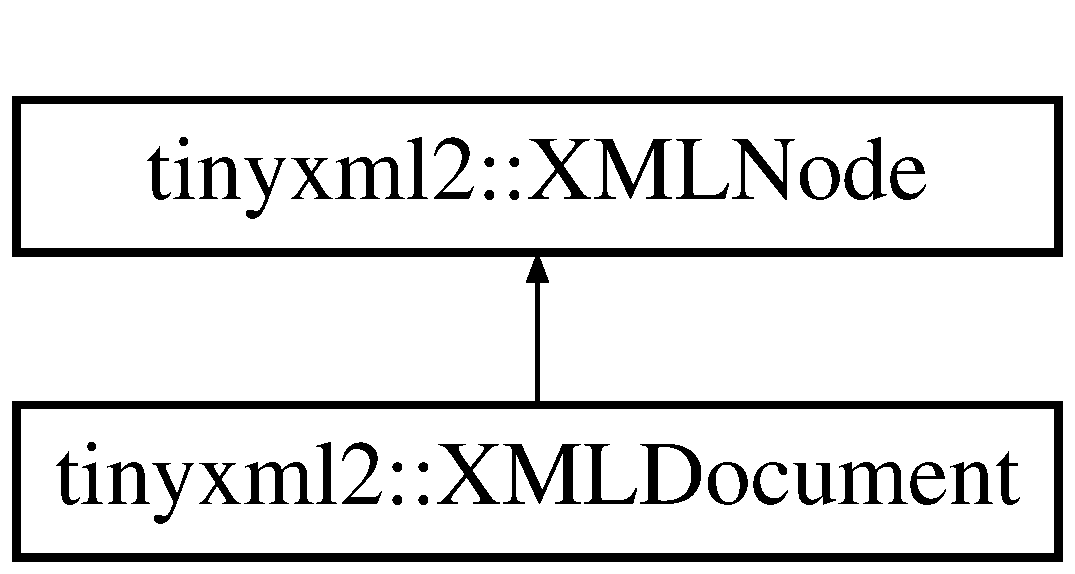
\includegraphics[height=2.000000cm]{classtinyxml2_1_1_x_m_l_document}
\end{center}
\end{figure}
\subsection*{Public Member Functions}
\begin{DoxyCompactItemize}
\item 
\hyperlink{classtinyxml2_1_1_x_m_l_document_af1574f76ebb619f25ef3f09eb2ba5188}{X\-M\-L\-Document} (bool process\-Entities=true, \hyperlink{namespacetinyxml2_a7f91d00f77360f850fd5da0861e27dd5}{Whitespace}=\hyperlink{namespacetinyxml2_a7f91d00f77360f850fd5da0861e27dd5a751769aa625fe5fe5286e9779edec56a}{P\-R\-E\-S\-E\-R\-V\-E\-\_\-\-W\-H\-I\-T\-E\-S\-P\-A\-C\-E})
\begin{DoxyCompactList}\small\item\em constructor \end{DoxyCompactList}\item 
\hyperlink{classtinyxml2_1_1_x_m_l_document_af37c47d8e2ba4b2fc81b21a77a32579b}{$\sim$\-X\-M\-L\-Document} ()
\item 
virtual \hyperlink{classtinyxml2_1_1_x_m_l_document}{X\-M\-L\-Document} $\ast$ \hyperlink{classtinyxml2_1_1_x_m_l_document_a3e185f880882bd978367bb55937735ec}{To\-Document} ()
\begin{DoxyCompactList}\small\item\em Safely cast to a Document, or null. \end{DoxyCompactList}\item 
virtual const \hyperlink{classtinyxml2_1_1_x_m_l_document}{X\-M\-L\-Document} $\ast$ \hyperlink{classtinyxml2_1_1_x_m_l_document_a15eb1a62afa18c66808031da647d1129}{To\-Document} () const 
\item 
\hyperlink{namespacetinyxml2_a1fbf88509c3ac88c09117b1947414e08}{X\-M\-L\-Error} \hyperlink{classtinyxml2_1_1_x_m_l_document_a1819bd34f540a7304c105a6232d25a1f}{Parse} (const char $\ast$xml, size\-\_\-t n\-Bytes=(size\-\_\-t)(-\/1))
\item 
\hyperlink{namespacetinyxml2_a1fbf88509c3ac88c09117b1947414e08}{X\-M\-L\-Error} \hyperlink{classtinyxml2_1_1_x_m_l_document_a2ebd4647a8af5fc6831b294ac26a150a}{Load\-File} (const char $\ast$filename)
\item 
\hyperlink{namespacetinyxml2_a1fbf88509c3ac88c09117b1947414e08}{X\-M\-L\-Error} \hyperlink{classtinyxml2_1_1_x_m_l_document_a5f1d330fad44c52f3d265338dd2a6dc2}{Load\-File} (F\-I\-L\-E $\ast$)
\item 
\hyperlink{namespacetinyxml2_a1fbf88509c3ac88c09117b1947414e08}{X\-M\-L\-Error} \hyperlink{classtinyxml2_1_1_x_m_l_document_a73ac416b4a2aa0952e841220eb3da18f}{Save\-File} (const char $\ast$filename, bool compact=false)
\item 
\hyperlink{namespacetinyxml2_a1fbf88509c3ac88c09117b1947414e08}{X\-M\-L\-Error} \hyperlink{classtinyxml2_1_1_x_m_l_document_a8b95779479a0035acc67b3a61dfe1b74}{Save\-File} (F\-I\-L\-E $\ast$fp, bool compact=false)
\item 
bool \hyperlink{classtinyxml2_1_1_x_m_l_document_adfcff7d0599cd520e9fcbb8891e1b678}{Process\-Entities} () const 
\item 
\hyperlink{namespacetinyxml2_a7f91d00f77360f850fd5da0861e27dd5}{Whitespace} \hyperlink{classtinyxml2_1_1_x_m_l_document_a94b3ea2f77c9ac831723984df5a02d01}{Whitespace\-Mode} () const 
\item 
bool \hyperlink{classtinyxml2_1_1_x_m_l_document_a530649e9de7e5aa8df9c37f66197fcb6}{Has\-B\-O\-M} () const 
\item 
void \hyperlink{classtinyxml2_1_1_x_m_l_document_a14419b698f7c4b140df4e80f3f0c93b0}{Set\-B\-O\-M} (bool use\-B\-O\-M)
\item 
\hyperlink{classtinyxml2_1_1_x_m_l_element}{X\-M\-L\-Element} $\ast$ \hyperlink{classtinyxml2_1_1_x_m_l_document_ad2b70320d3c2a071c2f36928edff3e1c}{Root\-Element} ()
\item 
const \hyperlink{classtinyxml2_1_1_x_m_l_element}{X\-M\-L\-Element} $\ast$ \hyperlink{classtinyxml2_1_1_x_m_l_document_a23a25b573d2adf3ee6075636c2a31c73}{Root\-Element} () const 
\item 
void \hyperlink{classtinyxml2_1_1_x_m_l_document_a686ea28672c0e0c60383ec28148c1ac0}{Print} (\hyperlink{classtinyxml2_1_1_x_m_l_printer}{X\-M\-L\-Printer} $\ast$streamer=0) const 
\item 
virtual bool \hyperlink{classtinyxml2_1_1_x_m_l_document_aa08503d24898bf9992ae5e5fb8b0cf87}{Accept} (\hyperlink{classtinyxml2_1_1_x_m_l_visitor}{X\-M\-L\-Visitor} $\ast$visitor) const 
\item 
\hyperlink{classtinyxml2_1_1_x_m_l_element}{X\-M\-L\-Element} $\ast$ \hyperlink{classtinyxml2_1_1_x_m_l_document_a3c335a700a43d7c363a393142a23f234}{New\-Element} (const char $\ast$name)
\item 
\hyperlink{classtinyxml2_1_1_x_m_l_comment}{X\-M\-L\-Comment} $\ast$ \hyperlink{classtinyxml2_1_1_x_m_l_document_a386df0befd06aadb5e0cd21381aa955a}{New\-Comment} (const char $\ast$comment)
\item 
\hyperlink{classtinyxml2_1_1_x_m_l_text}{X\-M\-L\-Text} $\ast$ \hyperlink{classtinyxml2_1_1_x_m_l_document_acece5de77a0819f2341b08c1e1ed9987}{New\-Text} (const char $\ast$text)
\item 
\hyperlink{classtinyxml2_1_1_x_m_l_declaration}{X\-M\-L\-Declaration} $\ast$ \hyperlink{classtinyxml2_1_1_x_m_l_document_ae519030c0262fa2daff8993681990e16}{New\-Declaration} (const char $\ast$text=0)
\item 
\hyperlink{classtinyxml2_1_1_x_m_l_unknown}{X\-M\-L\-Unknown} $\ast$ \hyperlink{classtinyxml2_1_1_x_m_l_document_a4954f502c5fd7f49de54c3c0c99bb73d}{New\-Unknown} (const char $\ast$text)
\item 
void \hyperlink{classtinyxml2_1_1_x_m_l_document_ac1d6e2c7fcc1a660624ac4f68e96380d}{Delete\-Node} (\hyperlink{classtinyxml2_1_1_x_m_l_node}{X\-M\-L\-Node} $\ast$node)
\item 
void \hyperlink{classtinyxml2_1_1_x_m_l_document_ae38d194e47336e4c96677ac77e2ac5d4}{Set\-Error} (\hyperlink{namespacetinyxml2_a1fbf88509c3ac88c09117b1947414e08}{X\-M\-L\-Error} error, const char $\ast$str1, const char $\ast$str2)
\item 
bool \hyperlink{classtinyxml2_1_1_x_m_l_document_abf0f9ac4c3aa5698a785937f71f7a69f}{Error} () const 
\begin{DoxyCompactList}\small\item\em Return true if there was an error parsing the document. \end{DoxyCompactList}\item 
\hyperlink{namespacetinyxml2_a1fbf88509c3ac88c09117b1947414e08}{X\-M\-L\-Error} \hyperlink{classtinyxml2_1_1_x_m_l_document_a34903418c9e83f27945c2c533839e350}{Error\-I\-D} () const 
\begin{DoxyCompactList}\small\item\em Return the error\-I\-D. \end{DoxyCompactList}\item 
const char $\ast$ \hyperlink{classtinyxml2_1_1_x_m_l_document_a016ccebecee36fe92084b5dfee6cc072}{Get\-Error\-Str1} () const 
\begin{DoxyCompactList}\small\item\em Return a possibly helpful diagnostic location or string. \end{DoxyCompactList}\item 
const char $\ast$ \hyperlink{classtinyxml2_1_1_x_m_l_document_a88f6b44bd019033bda28abd31fe257b2}{Get\-Error\-Str2} () const 
\begin{DoxyCompactList}\small\item\em Return a possibly helpful secondary diagnostic location or string. \end{DoxyCompactList}\item 
void \hyperlink{classtinyxml2_1_1_x_m_l_document_a7545cc9a9a67eee9307c001aa316a388}{Print\-Error} () const 
\begin{DoxyCompactList}\small\item\em If there is an error, print it to stdout. \end{DoxyCompactList}\item 
void \hyperlink{classtinyxml2_1_1_x_m_l_document_a65656b0b2cbc822708eb351504178aaf}{Clear} ()
\begin{DoxyCompactList}\small\item\em Clear the document, resetting it to the initial state. \end{DoxyCompactList}\item 
char $\ast$ \hyperlink{classtinyxml2_1_1_x_m_l_document_a25827d1bec509ad566a107e5853ed040}{Identify} (char $\ast$p, \hyperlink{classtinyxml2_1_1_x_m_l_node}{X\-M\-L\-Node} $\ast$$\ast$node)
\item 
virtual \hyperlink{classtinyxml2_1_1_x_m_l_node}{X\-M\-L\-Node} $\ast$ \hyperlink{classtinyxml2_1_1_x_m_l_document_a57c8511ed9f83aa3e20909a3db3f83d0}{Shallow\-Clone} (\hyperlink{classtinyxml2_1_1_x_m_l_document}{X\-M\-L\-Document} $\ast$) const 
\item 
virtual bool \hyperlink{classtinyxml2_1_1_x_m_l_document_a12eac66c6e45d074d5cc47319868cd66}{Shallow\-Equal} (const \hyperlink{classtinyxml2_1_1_x_m_l_node}{X\-M\-L\-Node} $\ast$) const 
\end{DoxyCompactItemize}
\subsection*{Friends}
\begin{DoxyCompactItemize}
\item 
class \hyperlink{classtinyxml2_1_1_x_m_l_document_ac2fba9b6e452829dd892f7392c24e0eb}{X\-M\-L\-Element}
\end{DoxyCompactItemize}
\subsection*{Additional Inherited Members}


\subsection{Detailed Description}
A Document binds together all the functionality. It can be saved, loaded, and printed to the screen. All Nodes are connected and allocated to a Document. If the Document is deleted, all its Nodes are also deleted. 

Definition at line 1428 of file tinyxml2.\-hpp.



\subsection{Constructor \& Destructor Documentation}
\hypertarget{classtinyxml2_1_1_x_m_l_document_af1574f76ebb619f25ef3f09eb2ba5188}{\index{tinyxml2\-::\-X\-M\-L\-Document@{tinyxml2\-::\-X\-M\-L\-Document}!X\-M\-L\-Document@{X\-M\-L\-Document}}
\index{X\-M\-L\-Document@{X\-M\-L\-Document}!tinyxml2::XMLDocument@{tinyxml2\-::\-X\-M\-L\-Document}}
\subsubsection[{X\-M\-L\-Document}]{\setlength{\rightskip}{0pt plus 5cm}tinyxml2\-::\-X\-M\-L\-Document\-::\-X\-M\-L\-Document (
\begin{DoxyParamCaption}
\item[{bool}]{process\-Entities = {\ttfamily true}, }
\item[{{\bf Whitespace}}]{whitespace = {\ttfamily {\bf P\-R\-E\-S\-E\-R\-V\-E\-\_\-\-W\-H\-I\-T\-E\-S\-P\-A\-C\-E}}}
\end{DoxyParamCaption}
)}}\label{classtinyxml2_1_1_x_m_l_document_af1574f76ebb619f25ef3f09eb2ba5188}


constructor 



Definition at line 1487 of file tinyxml2.\-cpp.

\hypertarget{classtinyxml2_1_1_x_m_l_document_af37c47d8e2ba4b2fc81b21a77a32579b}{\index{tinyxml2\-::\-X\-M\-L\-Document@{tinyxml2\-::\-X\-M\-L\-Document}!$\sim$\-X\-M\-L\-Document@{$\sim$\-X\-M\-L\-Document}}
\index{$\sim$\-X\-M\-L\-Document@{$\sim$\-X\-M\-L\-Document}!tinyxml2::XMLDocument@{tinyxml2\-::\-X\-M\-L\-Document}}
\subsubsection[{$\sim$\-X\-M\-L\-Document}]{\setlength{\rightskip}{0pt plus 5cm}tinyxml2\-::\-X\-M\-L\-Document\-::$\sim$\-X\-M\-L\-Document (
\begin{DoxyParamCaption}
{}
\end{DoxyParamCaption}
)}}\label{classtinyxml2_1_1_x_m_l_document_af37c47d8e2ba4b2fc81b21a77a32579b}


Definition at line 1501 of file tinyxml2.\-cpp.



\subsection{Member Function Documentation}
\hypertarget{classtinyxml2_1_1_x_m_l_document_aa08503d24898bf9992ae5e5fb8b0cf87}{\index{tinyxml2\-::\-X\-M\-L\-Document@{tinyxml2\-::\-X\-M\-L\-Document}!Accept@{Accept}}
\index{Accept@{Accept}!tinyxml2::XMLDocument@{tinyxml2\-::\-X\-M\-L\-Document}}
\subsubsection[{Accept}]{\setlength{\rightskip}{0pt plus 5cm}bool tinyxml2\-::\-X\-M\-L\-Document\-::\-Accept (
\begin{DoxyParamCaption}
\item[{{\bf X\-M\-L\-Visitor} $\ast$}]{visitor}
\end{DoxyParamCaption}
) const\hspace{0.3cm}{\ttfamily [virtual]}}}\label{classtinyxml2_1_1_x_m_l_document_aa08503d24898bf9992ae5e5fb8b0cf87}
Accept a hierarchical visit of the nodes in the Tiny\-X\-M\-L-\/2 D\-O\-M. Every node in the \hyperlink{namespace_x_m_l}{X\-M\-L} tree will be conditionally visited and the host will be called back via the \hyperlink{classtinyxml2_1_1_x_m_l_visitor}{X\-M\-L\-Visitor} interface.

This is essentially a S\-A\-X interface for Tiny\-X\-M\-L-\/2. (Note however it doesn't re-\/parse the \hyperlink{namespace_x_m_l}{X\-M\-L} for the callbacks, so the performance of Tiny\-X\-M\-L-\/2 is unchanged by using this interface versus any other.)

The interface has been based on ideas from\-:


\begin{DoxyItemize}
\item \href{http://www.saxproject.org/}{\tt http\-://www.\-saxproject.\-org/}
\item \href{http://c2.com/cgi/wiki?HierarchicalVisitorPattern}{\tt http\-://c2.\-com/cgi/wiki?\-Hierarchical\-Visitor\-Pattern}
\end{DoxyItemize}

Which are both good references for \char`\"{}visiting\char`\"{}.

An example of using \hyperlink{classtinyxml2_1_1_x_m_l_document_aa08503d24898bf9992ae5e5fb8b0cf87}{Accept()}\-: \begin{DoxyVerb}XMLPrinter printer;
tinyxmlDoc.Accept( &printer );
const char* xmlcstr = printer.CStr();
\end{DoxyVerb}
 

Implements \hyperlink{classtinyxml2_1_1_x_m_l_node_a81e66df0a44c67a7af17f3b77a152785}{tinyxml2\-::\-X\-M\-L\-Node}.



Definition at line 565 of file tinyxml2.\-cpp.

\hypertarget{classtinyxml2_1_1_x_m_l_document_a65656b0b2cbc822708eb351504178aaf}{\index{tinyxml2\-::\-X\-M\-L\-Document@{tinyxml2\-::\-X\-M\-L\-Document}!Clear@{Clear}}
\index{Clear@{Clear}!tinyxml2::XMLDocument@{tinyxml2\-::\-X\-M\-L\-Document}}
\subsubsection[{Clear}]{\setlength{\rightskip}{0pt plus 5cm}void tinyxml2\-::\-X\-M\-L\-Document\-::\-Clear (
\begin{DoxyParamCaption}
{}
\end{DoxyParamCaption}
)}}\label{classtinyxml2_1_1_x_m_l_document_a65656b0b2cbc822708eb351504178aaf}


Clear the document, resetting it to the initial state. 



Definition at line 1524 of file tinyxml2.\-cpp.

\hypertarget{classtinyxml2_1_1_x_m_l_document_ac1d6e2c7fcc1a660624ac4f68e96380d}{\index{tinyxml2\-::\-X\-M\-L\-Document@{tinyxml2\-::\-X\-M\-L\-Document}!Delete\-Node@{Delete\-Node}}
\index{Delete\-Node@{Delete\-Node}!tinyxml2::XMLDocument@{tinyxml2\-::\-X\-M\-L\-Document}}
\subsubsection[{Delete\-Node}]{\setlength{\rightskip}{0pt plus 5cm}void tinyxml2\-::\-X\-M\-L\-Document\-::\-Delete\-Node (
\begin{DoxyParamCaption}
\item[{{\bf X\-M\-L\-Node} $\ast$}]{node}
\end{DoxyParamCaption}
)\hspace{0.3cm}{\ttfamily [inline]}}}\label{classtinyxml2_1_1_x_m_l_document_ac1d6e2c7fcc1a660624ac4f68e96380d}
Delete a node associated with this document. It will be unlinked from the D\-O\-M. 

Definition at line 1574 of file tinyxml2.\-hpp.

\hypertarget{classtinyxml2_1_1_x_m_l_document_abf0f9ac4c3aa5698a785937f71f7a69f}{\index{tinyxml2\-::\-X\-M\-L\-Document@{tinyxml2\-::\-X\-M\-L\-Document}!Error@{Error}}
\index{Error@{Error}!tinyxml2::XMLDocument@{tinyxml2\-::\-X\-M\-L\-Document}}
\subsubsection[{Error}]{\setlength{\rightskip}{0pt plus 5cm}bool tinyxml2\-::\-X\-M\-L\-Document\-::\-Error (
\begin{DoxyParamCaption}
{}
\end{DoxyParamCaption}
) const\hspace{0.3cm}{\ttfamily [inline]}}}\label{classtinyxml2_1_1_x_m_l_document_abf0f9ac4c3aa5698a785937f71f7a69f}


Return true if there was an error parsing the document. 



Definition at line 1581 of file tinyxml2.\-hpp.

\hypertarget{classtinyxml2_1_1_x_m_l_document_a34903418c9e83f27945c2c533839e350}{\index{tinyxml2\-::\-X\-M\-L\-Document@{tinyxml2\-::\-X\-M\-L\-Document}!Error\-I\-D@{Error\-I\-D}}
\index{Error\-I\-D@{Error\-I\-D}!tinyxml2::XMLDocument@{tinyxml2\-::\-X\-M\-L\-Document}}
\subsubsection[{Error\-I\-D}]{\setlength{\rightskip}{0pt plus 5cm}{\bf X\-M\-L\-Error} tinyxml2\-::\-X\-M\-L\-Document\-::\-Error\-I\-D (
\begin{DoxyParamCaption}
{}
\end{DoxyParamCaption}
) const\hspace{0.3cm}{\ttfamily [inline]}}}\label{classtinyxml2_1_1_x_m_l_document_a34903418c9e83f27945c2c533839e350}


Return the error\-I\-D. 



Definition at line 1585 of file tinyxml2.\-hpp.

\hypertarget{classtinyxml2_1_1_x_m_l_document_a016ccebecee36fe92084b5dfee6cc072}{\index{tinyxml2\-::\-X\-M\-L\-Document@{tinyxml2\-::\-X\-M\-L\-Document}!Get\-Error\-Str1@{Get\-Error\-Str1}}
\index{Get\-Error\-Str1@{Get\-Error\-Str1}!tinyxml2::XMLDocument@{tinyxml2\-::\-X\-M\-L\-Document}}
\subsubsection[{Get\-Error\-Str1}]{\setlength{\rightskip}{0pt plus 5cm}const char$\ast$ tinyxml2\-::\-X\-M\-L\-Document\-::\-Get\-Error\-Str1 (
\begin{DoxyParamCaption}
{}
\end{DoxyParamCaption}
) const\hspace{0.3cm}{\ttfamily [inline]}}}\label{classtinyxml2_1_1_x_m_l_document_a016ccebecee36fe92084b5dfee6cc072}


Return a possibly helpful diagnostic location or string. 



Definition at line 1589 of file tinyxml2.\-hpp.

\hypertarget{classtinyxml2_1_1_x_m_l_document_a88f6b44bd019033bda28abd31fe257b2}{\index{tinyxml2\-::\-X\-M\-L\-Document@{tinyxml2\-::\-X\-M\-L\-Document}!Get\-Error\-Str2@{Get\-Error\-Str2}}
\index{Get\-Error\-Str2@{Get\-Error\-Str2}!tinyxml2::XMLDocument@{tinyxml2\-::\-X\-M\-L\-Document}}
\subsubsection[{Get\-Error\-Str2}]{\setlength{\rightskip}{0pt plus 5cm}const char$\ast$ tinyxml2\-::\-X\-M\-L\-Document\-::\-Get\-Error\-Str2 (
\begin{DoxyParamCaption}
{}
\end{DoxyParamCaption}
) const\hspace{0.3cm}{\ttfamily [inline]}}}\label{classtinyxml2_1_1_x_m_l_document_a88f6b44bd019033bda28abd31fe257b2}


Return a possibly helpful secondary diagnostic location or string. 



Definition at line 1593 of file tinyxml2.\-hpp.

\hypertarget{classtinyxml2_1_1_x_m_l_document_a530649e9de7e5aa8df9c37f66197fcb6}{\index{tinyxml2\-::\-X\-M\-L\-Document@{tinyxml2\-::\-X\-M\-L\-Document}!Has\-B\-O\-M@{Has\-B\-O\-M}}
\index{Has\-B\-O\-M@{Has\-B\-O\-M}!tinyxml2::XMLDocument@{tinyxml2\-::\-X\-M\-L\-Document}}
\subsubsection[{Has\-B\-O\-M}]{\setlength{\rightskip}{0pt plus 5cm}bool tinyxml2\-::\-X\-M\-L\-Document\-::\-Has\-B\-O\-M (
\begin{DoxyParamCaption}
{}
\end{DoxyParamCaption}
) const\hspace{0.3cm}{\ttfamily [inline]}}}\label{classtinyxml2_1_1_x_m_l_document_a530649e9de7e5aa8df9c37f66197fcb6}
Returns true if this document has a leading Byte Order Mark of U\-T\-F8. 

Definition at line 1497 of file tinyxml2.\-hpp.

\hypertarget{classtinyxml2_1_1_x_m_l_document_a25827d1bec509ad566a107e5853ed040}{\index{tinyxml2\-::\-X\-M\-L\-Document@{tinyxml2\-::\-X\-M\-L\-Document}!Identify@{Identify}}
\index{Identify@{Identify}!tinyxml2::XMLDocument@{tinyxml2\-::\-X\-M\-L\-Document}}
\subsubsection[{Identify}]{\setlength{\rightskip}{0pt plus 5cm}char $\ast$ tinyxml2\-::\-X\-M\-L\-Document\-::\-Identify (
\begin{DoxyParamCaption}
\item[{char $\ast$}]{p, }
\item[{{\bf X\-M\-L\-Node} $\ast$$\ast$}]{node}
\end{DoxyParamCaption}
)}}\label{classtinyxml2_1_1_x_m_l_document_a25827d1bec509ad566a107e5853ed040}


Definition at line 490 of file tinyxml2.\-cpp.

\hypertarget{classtinyxml2_1_1_x_m_l_document_a2ebd4647a8af5fc6831b294ac26a150a}{\index{tinyxml2\-::\-X\-M\-L\-Document@{tinyxml2\-::\-X\-M\-L\-Document}!Load\-File@{Load\-File}}
\index{Load\-File@{Load\-File}!tinyxml2::XMLDocument@{tinyxml2\-::\-X\-M\-L\-Document}}
\subsubsection[{Load\-File}]{\setlength{\rightskip}{0pt plus 5cm}{\bf X\-M\-L\-Error} tinyxml2\-::\-X\-M\-L\-Document\-::\-Load\-File (
\begin{DoxyParamCaption}
\item[{const char $\ast$}]{filename}
\end{DoxyParamCaption}
)}}\label{classtinyxml2_1_1_x_m_l_document_a2ebd4647a8af5fc6831b294ac26a150a}
Load an \hyperlink{namespace_x_m_l}{X\-M\-L} file from disk. Returns X\-M\-L\-\_\-\-N\-O\-\_\-\-E\-R\-R\-O\-R (0) on success, or an error\-I\-D. 

Definition at line 1582 of file tinyxml2.\-cpp.

\hypertarget{classtinyxml2_1_1_x_m_l_document_a5f1d330fad44c52f3d265338dd2a6dc2}{\index{tinyxml2\-::\-X\-M\-L\-Document@{tinyxml2\-::\-X\-M\-L\-Document}!Load\-File@{Load\-File}}
\index{Load\-File@{Load\-File}!tinyxml2::XMLDocument@{tinyxml2\-::\-X\-M\-L\-Document}}
\subsubsection[{Load\-File}]{\setlength{\rightskip}{0pt plus 5cm}{\bf X\-M\-L\-Error} tinyxml2\-::\-X\-M\-L\-Document\-::\-Load\-File (
\begin{DoxyParamCaption}
\item[{F\-I\-L\-E $\ast$}]{fp}
\end{DoxyParamCaption}
)}}\label{classtinyxml2_1_1_x_m_l_document_a5f1d330fad44c52f3d265338dd2a6dc2}
Load an \hyperlink{namespace_x_m_l}{X\-M\-L} file from disk. You are responsible for providing and closing the F\-I\-L\-E$\ast$.

Returns X\-M\-L\-\_\-\-N\-O\-\_\-\-E\-R\-R\-O\-R (0) on success, or an error\-I\-D. 

Definition at line 1603 of file tinyxml2.\-cpp.

\hypertarget{classtinyxml2_1_1_x_m_l_document_a386df0befd06aadb5e0cd21381aa955a}{\index{tinyxml2\-::\-X\-M\-L\-Document@{tinyxml2\-::\-X\-M\-L\-Document}!New\-Comment@{New\-Comment}}
\index{New\-Comment@{New\-Comment}!tinyxml2::XMLDocument@{tinyxml2\-::\-X\-M\-L\-Document}}
\subsubsection[{New\-Comment}]{\setlength{\rightskip}{0pt plus 5cm}{\bf X\-M\-L\-Comment} $\ast$ tinyxml2\-::\-X\-M\-L\-Document\-::\-New\-Comment (
\begin{DoxyParamCaption}
\item[{const char $\ast$}]{comment}
\end{DoxyParamCaption}
)}}\label{classtinyxml2_1_1_x_m_l_document_a386df0befd06aadb5e0cd21381aa955a}
Create a new Comment associated with this Document. The memory for the Comment is managed by the Document. 

Definition at line 1546 of file tinyxml2.\-cpp.

\hypertarget{classtinyxml2_1_1_x_m_l_document_ae519030c0262fa2daff8993681990e16}{\index{tinyxml2\-::\-X\-M\-L\-Document@{tinyxml2\-::\-X\-M\-L\-Document}!New\-Declaration@{New\-Declaration}}
\index{New\-Declaration@{New\-Declaration}!tinyxml2::XMLDocument@{tinyxml2\-::\-X\-M\-L\-Document}}
\subsubsection[{New\-Declaration}]{\setlength{\rightskip}{0pt plus 5cm}{\bf X\-M\-L\-Declaration} $\ast$ tinyxml2\-::\-X\-M\-L\-Document\-::\-New\-Declaration (
\begin{DoxyParamCaption}
\item[{const char $\ast$}]{text = {\ttfamily 0}}
\end{DoxyParamCaption}
)}}\label{classtinyxml2_1_1_x_m_l_document_ae519030c0262fa2daff8993681990e16}
Create a new Declaration associated with this Document. The memory for the object is managed by the Document.

If the 'text' param is null, the standard declaration is used.\-: \begin{DoxyVerb}    <?xml version="1.0" encoding="UTF-8"?>
\end{DoxyVerb}
 

Definition at line 1564 of file tinyxml2.\-cpp.

\hypertarget{classtinyxml2_1_1_x_m_l_document_a3c335a700a43d7c363a393142a23f234}{\index{tinyxml2\-::\-X\-M\-L\-Document@{tinyxml2\-::\-X\-M\-L\-Document}!New\-Element@{New\-Element}}
\index{New\-Element@{New\-Element}!tinyxml2::XMLDocument@{tinyxml2\-::\-X\-M\-L\-Document}}
\subsubsection[{New\-Element}]{\setlength{\rightskip}{0pt plus 5cm}{\bf X\-M\-L\-Element} $\ast$ tinyxml2\-::\-X\-M\-L\-Document\-::\-New\-Element (
\begin{DoxyParamCaption}
\item[{const char $\ast$}]{name}
\end{DoxyParamCaption}
)}}\label{classtinyxml2_1_1_x_m_l_document_a3c335a700a43d7c363a393142a23f234}
Create a new Element associated with this Document. The memory for the Element is managed by the Document. 

Definition at line 1537 of file tinyxml2.\-cpp.

\hypertarget{classtinyxml2_1_1_x_m_l_document_acece5de77a0819f2341b08c1e1ed9987}{\index{tinyxml2\-::\-X\-M\-L\-Document@{tinyxml2\-::\-X\-M\-L\-Document}!New\-Text@{New\-Text}}
\index{New\-Text@{New\-Text}!tinyxml2::XMLDocument@{tinyxml2\-::\-X\-M\-L\-Document}}
\subsubsection[{New\-Text}]{\setlength{\rightskip}{0pt plus 5cm}{\bf X\-M\-L\-Text} $\ast$ tinyxml2\-::\-X\-M\-L\-Document\-::\-New\-Text (
\begin{DoxyParamCaption}
\item[{const char $\ast$}]{text}
\end{DoxyParamCaption}
)}}\label{classtinyxml2_1_1_x_m_l_document_acece5de77a0819f2341b08c1e1ed9987}
Create a new Text associated with this Document. The memory for the Text is managed by the Document. 

Definition at line 1555 of file tinyxml2.\-cpp.

\hypertarget{classtinyxml2_1_1_x_m_l_document_a4954f502c5fd7f49de54c3c0c99bb73d}{\index{tinyxml2\-::\-X\-M\-L\-Document@{tinyxml2\-::\-X\-M\-L\-Document}!New\-Unknown@{New\-Unknown}}
\index{New\-Unknown@{New\-Unknown}!tinyxml2::XMLDocument@{tinyxml2\-::\-X\-M\-L\-Document}}
\subsubsection[{New\-Unknown}]{\setlength{\rightskip}{0pt plus 5cm}{\bf X\-M\-L\-Unknown} $\ast$ tinyxml2\-::\-X\-M\-L\-Document\-::\-New\-Unknown (
\begin{DoxyParamCaption}
\item[{const char $\ast$}]{text}
\end{DoxyParamCaption}
)}}\label{classtinyxml2_1_1_x_m_l_document_a4954f502c5fd7f49de54c3c0c99bb73d}
Create a new Unknown associated with this Document. The memory for the object is managed by the Document. 

Definition at line 1573 of file tinyxml2.\-cpp.

\hypertarget{classtinyxml2_1_1_x_m_l_document_a1819bd34f540a7304c105a6232d25a1f}{\index{tinyxml2\-::\-X\-M\-L\-Document@{tinyxml2\-::\-X\-M\-L\-Document}!Parse@{Parse}}
\index{Parse@{Parse}!tinyxml2::XMLDocument@{tinyxml2\-::\-X\-M\-L\-Document}}
\subsubsection[{Parse}]{\setlength{\rightskip}{0pt plus 5cm}{\bf X\-M\-L\-Error} tinyxml2\-::\-X\-M\-L\-Document\-::\-Parse (
\begin{DoxyParamCaption}
\item[{const char $\ast$}]{xml, }
\item[{size\-\_\-t}]{n\-Bytes = {\ttfamily (size\-\_\-t)(-\/1)}}
\end{DoxyParamCaption}
)}}\label{classtinyxml2_1_1_x_m_l_document_a1819bd34f540a7304c105a6232d25a1f}
Parse an \hyperlink{namespace_x_m_l}{X\-M\-L} file from a character string. Returns X\-M\-L\-\_\-\-N\-O\-\_\-\-E\-R\-R\-O\-R (0) on success, or an error\-I\-D.

You may optionally pass in the 'n\-Bytes', which is the number of bytes which will be parsed. If not specified, Tiny\-X\-M\-L-\/2 will assume 'xml' points to a null terminated string. 

Definition at line 1665 of file tinyxml2.\-cpp.

\hypertarget{classtinyxml2_1_1_x_m_l_document_a686ea28672c0e0c60383ec28148c1ac0}{\index{tinyxml2\-::\-X\-M\-L\-Document@{tinyxml2\-::\-X\-M\-L\-Document}!Print@{Print}}
\index{Print@{Print}!tinyxml2::XMLDocument@{tinyxml2\-::\-X\-M\-L\-Document}}
\subsubsection[{Print}]{\setlength{\rightskip}{0pt plus 5cm}void tinyxml2\-::\-X\-M\-L\-Document\-::\-Print (
\begin{DoxyParamCaption}
\item[{{\bf X\-M\-L\-Printer} $\ast$}]{streamer = {\ttfamily 0}}
\end{DoxyParamCaption}
) const}}\label{classtinyxml2_1_1_x_m_l_document_a686ea28672c0e0c60383ec28148c1ac0}
Print the Document. If the Printer is not provided, it will print to stdout. If you provide Printer, this can print to a file\-: \begin{DoxyVerb}XMLPrinter printer( fp );
doc.Print( &printer );
\end{DoxyVerb}


Or you can use a printer to print to memory\-: \begin{DoxyVerb}XMLPrinter printer;
doc.Print( &printer );
// printer.CStr() has a const char* to the XML
\end{DoxyVerb}
 

Definition at line 1694 of file tinyxml2.\-cpp.

\hypertarget{classtinyxml2_1_1_x_m_l_document_a7545cc9a9a67eee9307c001aa316a388}{\index{tinyxml2\-::\-X\-M\-L\-Document@{tinyxml2\-::\-X\-M\-L\-Document}!Print\-Error@{Print\-Error}}
\index{Print\-Error@{Print\-Error}!tinyxml2::XMLDocument@{tinyxml2\-::\-X\-M\-L\-Document}}
\subsubsection[{Print\-Error}]{\setlength{\rightskip}{0pt plus 5cm}void tinyxml2\-::\-X\-M\-L\-Document\-::\-Print\-Error (
\begin{DoxyParamCaption}
{}
\end{DoxyParamCaption}
) const}}\label{classtinyxml2_1_1_x_m_l_document_a7545cc9a9a67eee9307c001aa316a388}


If there is an error, print it to stdout. 



Definition at line 1712 of file tinyxml2.\-cpp.

\hypertarget{classtinyxml2_1_1_x_m_l_document_adfcff7d0599cd520e9fcbb8891e1b678}{\index{tinyxml2\-::\-X\-M\-L\-Document@{tinyxml2\-::\-X\-M\-L\-Document}!Process\-Entities@{Process\-Entities}}
\index{Process\-Entities@{Process\-Entities}!tinyxml2::XMLDocument@{tinyxml2\-::\-X\-M\-L\-Document}}
\subsubsection[{Process\-Entities}]{\setlength{\rightskip}{0pt plus 5cm}bool tinyxml2\-::\-X\-M\-L\-Document\-::\-Process\-Entities (
\begin{DoxyParamCaption}
{}
\end{DoxyParamCaption}
) const\hspace{0.3cm}{\ttfamily [inline]}}}\label{classtinyxml2_1_1_x_m_l_document_adfcff7d0599cd520e9fcbb8891e1b678}


Definition at line 1487 of file tinyxml2.\-hpp.

\hypertarget{classtinyxml2_1_1_x_m_l_document_ad2b70320d3c2a071c2f36928edff3e1c}{\index{tinyxml2\-::\-X\-M\-L\-Document@{tinyxml2\-::\-X\-M\-L\-Document}!Root\-Element@{Root\-Element}}
\index{Root\-Element@{Root\-Element}!tinyxml2::XMLDocument@{tinyxml2\-::\-X\-M\-L\-Document}}
\subsubsection[{Root\-Element}]{\setlength{\rightskip}{0pt plus 5cm}{\bf X\-M\-L\-Element}$\ast$ tinyxml2\-::\-X\-M\-L\-Document\-::\-Root\-Element (
\begin{DoxyParamCaption}
{}
\end{DoxyParamCaption}
)\hspace{0.3cm}{\ttfamily [inline]}}}\label{classtinyxml2_1_1_x_m_l_document_ad2b70320d3c2a071c2f36928edff3e1c}
Return the root element of D\-O\-M. Equivalent to \hyperlink{classtinyxml2_1_1_x_m_l_node_a20f48e99b03e9c17487944f229bee130}{First\-Child\-Element()}. To get the first node, use \hyperlink{classtinyxml2_1_1_x_m_l_node_a2d6c70c475146b48bc93a7fafdeff5e0}{First\-Child()}. 

Definition at line 1509 of file tinyxml2.\-hpp.

\hypertarget{classtinyxml2_1_1_x_m_l_document_a23a25b573d2adf3ee6075636c2a31c73}{\index{tinyxml2\-::\-X\-M\-L\-Document@{tinyxml2\-::\-X\-M\-L\-Document}!Root\-Element@{Root\-Element}}
\index{Root\-Element@{Root\-Element}!tinyxml2::XMLDocument@{tinyxml2\-::\-X\-M\-L\-Document}}
\subsubsection[{Root\-Element}]{\setlength{\rightskip}{0pt plus 5cm}const {\bf X\-M\-L\-Element}$\ast$ tinyxml2\-::\-X\-M\-L\-Document\-::\-Root\-Element (
\begin{DoxyParamCaption}
{}
\end{DoxyParamCaption}
) const\hspace{0.3cm}{\ttfamily [inline]}}}\label{classtinyxml2_1_1_x_m_l_document_a23a25b573d2adf3ee6075636c2a31c73}


Definition at line 1512 of file tinyxml2.\-hpp.

\hypertarget{classtinyxml2_1_1_x_m_l_document_a73ac416b4a2aa0952e841220eb3da18f}{\index{tinyxml2\-::\-X\-M\-L\-Document@{tinyxml2\-::\-X\-M\-L\-Document}!Save\-File@{Save\-File}}
\index{Save\-File@{Save\-File}!tinyxml2::XMLDocument@{tinyxml2\-::\-X\-M\-L\-Document}}
\subsubsection[{Save\-File}]{\setlength{\rightskip}{0pt plus 5cm}{\bf X\-M\-L\-Error} tinyxml2\-::\-X\-M\-L\-Document\-::\-Save\-File (
\begin{DoxyParamCaption}
\item[{const char $\ast$}]{filename, }
\item[{bool}]{compact = {\ttfamily false}}
\end{DoxyParamCaption}
)}}\label{classtinyxml2_1_1_x_m_l_document_a73ac416b4a2aa0952e841220eb3da18f}
Save the \hyperlink{namespace_x_m_l}{X\-M\-L} file to disk. Returns X\-M\-L\-\_\-\-N\-O\-\_\-\-E\-R\-R\-O\-R (0) on success, or an error\-I\-D. 

Definition at line 1638 of file tinyxml2.\-cpp.

\hypertarget{classtinyxml2_1_1_x_m_l_document_a8b95779479a0035acc67b3a61dfe1b74}{\index{tinyxml2\-::\-X\-M\-L\-Document@{tinyxml2\-::\-X\-M\-L\-Document}!Save\-File@{Save\-File}}
\index{Save\-File@{Save\-File}!tinyxml2::XMLDocument@{tinyxml2\-::\-X\-M\-L\-Document}}
\subsubsection[{Save\-File}]{\setlength{\rightskip}{0pt plus 5cm}{\bf X\-M\-L\-Error} tinyxml2\-::\-X\-M\-L\-Document\-::\-Save\-File (
\begin{DoxyParamCaption}
\item[{F\-I\-L\-E $\ast$}]{fp, }
\item[{bool}]{compact = {\ttfamily false}}
\end{DoxyParamCaption}
)}}\label{classtinyxml2_1_1_x_m_l_document_a8b95779479a0035acc67b3a61dfe1b74}
Save the \hyperlink{namespace_x_m_l}{X\-M\-L} file to disk. You are responsible for providing and closing the F\-I\-L\-E$\ast$.

Returns X\-M\-L\-\_\-\-N\-O\-\_\-\-E\-R\-R\-O\-R (0) on success, or an error\-I\-D. 

Definition at line 1657 of file tinyxml2.\-cpp.

\hypertarget{classtinyxml2_1_1_x_m_l_document_a14419b698f7c4b140df4e80f3f0c93b0}{\index{tinyxml2\-::\-X\-M\-L\-Document@{tinyxml2\-::\-X\-M\-L\-Document}!Set\-B\-O\-M@{Set\-B\-O\-M}}
\index{Set\-B\-O\-M@{Set\-B\-O\-M}!tinyxml2::XMLDocument@{tinyxml2\-::\-X\-M\-L\-Document}}
\subsubsection[{Set\-B\-O\-M}]{\setlength{\rightskip}{0pt plus 5cm}void tinyxml2\-::\-X\-M\-L\-Document\-::\-Set\-B\-O\-M (
\begin{DoxyParamCaption}
\item[{bool}]{use\-B\-O\-M}
\end{DoxyParamCaption}
)\hspace{0.3cm}{\ttfamily [inline]}}}\label{classtinyxml2_1_1_x_m_l_document_a14419b698f7c4b140df4e80f3f0c93b0}
Sets whether to write the B\-O\-M when writing the file. 

Definition at line 1502 of file tinyxml2.\-hpp.

\hypertarget{classtinyxml2_1_1_x_m_l_document_ae38d194e47336e4c96677ac77e2ac5d4}{\index{tinyxml2\-::\-X\-M\-L\-Document@{tinyxml2\-::\-X\-M\-L\-Document}!Set\-Error@{Set\-Error}}
\index{Set\-Error@{Set\-Error}!tinyxml2::XMLDocument@{tinyxml2\-::\-X\-M\-L\-Document}}
\subsubsection[{Set\-Error}]{\setlength{\rightskip}{0pt plus 5cm}void tinyxml2\-::\-X\-M\-L\-Document\-::\-Set\-Error (
\begin{DoxyParamCaption}
\item[{{\bf X\-M\-L\-Error}}]{error, }
\item[{const char $\ast$}]{str1, }
\item[{const char $\ast$}]{str2}
\end{DoxyParamCaption}
)}}\label{classtinyxml2_1_1_x_m_l_document_ae38d194e47336e4c96677ac77e2ac5d4}


Definition at line 1704 of file tinyxml2.\-cpp.

\hypertarget{classtinyxml2_1_1_x_m_l_document_a57c8511ed9f83aa3e20909a3db3f83d0}{\index{tinyxml2\-::\-X\-M\-L\-Document@{tinyxml2\-::\-X\-M\-L\-Document}!Shallow\-Clone@{Shallow\-Clone}}
\index{Shallow\-Clone@{Shallow\-Clone}!tinyxml2::XMLDocument@{tinyxml2\-::\-X\-M\-L\-Document}}
\subsubsection[{Shallow\-Clone}]{\setlength{\rightskip}{0pt plus 5cm}virtual {\bf X\-M\-L\-Node}$\ast$ tinyxml2\-::\-X\-M\-L\-Document\-::\-Shallow\-Clone (
\begin{DoxyParamCaption}
\item[{{\bf X\-M\-L\-Document} $\ast$}]{document}
\end{DoxyParamCaption}
) const\hspace{0.3cm}{\ttfamily [inline]}, {\ttfamily [virtual]}}}\label{classtinyxml2_1_1_x_m_l_document_a57c8511ed9f83aa3e20909a3db3f83d0}
Make a copy of this node, but not its children. You may pass in a Document pointer that will be the owner of the new Node. If the 'document' is null, then the node returned will be allocated from the current Document. (this-\/$>$\hyperlink{classtinyxml2_1_1_x_m_l_node_af343d1ef0b45c0020e62d784d7e67a68}{Get\-Document()})

Note\-: if called on a \hyperlink{classtinyxml2_1_1_x_m_l_document}{X\-M\-L\-Document}, this will return null. 

Implements \hyperlink{classtinyxml2_1_1_x_m_l_node_a8402cbd3129d20e9e6024bbcc0531283}{tinyxml2\-::\-X\-M\-L\-Node}.



Definition at line 1605 of file tinyxml2.\-hpp.

\hypertarget{classtinyxml2_1_1_x_m_l_document_a12eac66c6e45d074d5cc47319868cd66}{\index{tinyxml2\-::\-X\-M\-L\-Document@{tinyxml2\-::\-X\-M\-L\-Document}!Shallow\-Equal@{Shallow\-Equal}}
\index{Shallow\-Equal@{Shallow\-Equal}!tinyxml2::XMLDocument@{tinyxml2\-::\-X\-M\-L\-Document}}
\subsubsection[{Shallow\-Equal}]{\setlength{\rightskip}{0pt plus 5cm}virtual bool tinyxml2\-::\-X\-M\-L\-Document\-::\-Shallow\-Equal (
\begin{DoxyParamCaption}
\item[{const {\bf X\-M\-L\-Node} $\ast$}]{compare}
\end{DoxyParamCaption}
) const\hspace{0.3cm}{\ttfamily [inline]}, {\ttfamily [virtual]}}}\label{classtinyxml2_1_1_x_m_l_document_a12eac66c6e45d074d5cc47319868cd66}
Test if 2 nodes are the same, but don't test children. The 2 nodes do not need to be in the same Document.

Note\-: if called on a \hyperlink{classtinyxml2_1_1_x_m_l_document}{X\-M\-L\-Document}, this will return false. 

Implements \hyperlink{classtinyxml2_1_1_x_m_l_node_a7ce18b751c3ea09eac292dca264f9226}{tinyxml2\-::\-X\-M\-L\-Node}.



Definition at line 1608 of file tinyxml2.\-hpp.

\hypertarget{classtinyxml2_1_1_x_m_l_document_a3e185f880882bd978367bb55937735ec}{\index{tinyxml2\-::\-X\-M\-L\-Document@{tinyxml2\-::\-X\-M\-L\-Document}!To\-Document@{To\-Document}}
\index{To\-Document@{To\-Document}!tinyxml2::XMLDocument@{tinyxml2\-::\-X\-M\-L\-Document}}
\subsubsection[{To\-Document}]{\setlength{\rightskip}{0pt plus 5cm}virtual {\bf X\-M\-L\-Document}$\ast$ tinyxml2\-::\-X\-M\-L\-Document\-::\-To\-Document (
\begin{DoxyParamCaption}
{}
\end{DoxyParamCaption}
)\hspace{0.3cm}{\ttfamily [inline]}, {\ttfamily [virtual]}}}\label{classtinyxml2_1_1_x_m_l_document_a3e185f880882bd978367bb55937735ec}


Safely cast to a Document, or null. 



Reimplemented from \hyperlink{classtinyxml2_1_1_x_m_l_node_a836e2966ed736fc3c94f70e12a2a3357}{tinyxml2\-::\-X\-M\-L\-Node}.



Definition at line 1436 of file tinyxml2.\-hpp.

\hypertarget{classtinyxml2_1_1_x_m_l_document_a15eb1a62afa18c66808031da647d1129}{\index{tinyxml2\-::\-X\-M\-L\-Document@{tinyxml2\-::\-X\-M\-L\-Document}!To\-Document@{To\-Document}}
\index{To\-Document@{To\-Document}!tinyxml2::XMLDocument@{tinyxml2\-::\-X\-M\-L\-Document}}
\subsubsection[{To\-Document}]{\setlength{\rightskip}{0pt plus 5cm}virtual const {\bf X\-M\-L\-Document}$\ast$ tinyxml2\-::\-X\-M\-L\-Document\-::\-To\-Document (
\begin{DoxyParamCaption}
{}
\end{DoxyParamCaption}
) const\hspace{0.3cm}{\ttfamily [inline]}, {\ttfamily [virtual]}}}\label{classtinyxml2_1_1_x_m_l_document_a15eb1a62afa18c66808031da647d1129}


Reimplemented from \hyperlink{classtinyxml2_1_1_x_m_l_node_a3ff975733a17d6ced3539b45544c8bf6}{tinyxml2\-::\-X\-M\-L\-Node}.



Definition at line 1439 of file tinyxml2.\-hpp.

\hypertarget{classtinyxml2_1_1_x_m_l_document_a94b3ea2f77c9ac831723984df5a02d01}{\index{tinyxml2\-::\-X\-M\-L\-Document@{tinyxml2\-::\-X\-M\-L\-Document}!Whitespace\-Mode@{Whitespace\-Mode}}
\index{Whitespace\-Mode@{Whitespace\-Mode}!tinyxml2::XMLDocument@{tinyxml2\-::\-X\-M\-L\-Document}}
\subsubsection[{Whitespace\-Mode}]{\setlength{\rightskip}{0pt plus 5cm}{\bf Whitespace} tinyxml2\-::\-X\-M\-L\-Document\-::\-Whitespace\-Mode (
\begin{DoxyParamCaption}
{}
\end{DoxyParamCaption}
) const\hspace{0.3cm}{\ttfamily [inline]}}}\label{classtinyxml2_1_1_x_m_l_document_a94b3ea2f77c9ac831723984df5a02d01}


Definition at line 1490 of file tinyxml2.\-hpp.



\subsection{Friends And Related Function Documentation}
\hypertarget{classtinyxml2_1_1_x_m_l_document_ac2fba9b6e452829dd892f7392c24e0eb}{\index{tinyxml2\-::\-X\-M\-L\-Document@{tinyxml2\-::\-X\-M\-L\-Document}!X\-M\-L\-Element@{X\-M\-L\-Element}}
\index{X\-M\-L\-Element@{X\-M\-L\-Element}!tinyxml2::XMLDocument@{tinyxml2\-::\-X\-M\-L\-Document}}
\subsubsection[{X\-M\-L\-Element}]{\setlength{\rightskip}{0pt plus 5cm}friend class {\bf X\-M\-L\-Element}\hspace{0.3cm}{\ttfamily [friend]}}}\label{classtinyxml2_1_1_x_m_l_document_ac2fba9b6e452829dd892f7392c24e0eb}


Definition at line 1430 of file tinyxml2.\-hpp.



The documentation for this class was generated from the following files\-:\begin{DoxyCompactItemize}
\item 
Glide/\hyperlink{tinyxml2_8hpp}{tinyxml2.\-hpp}\item 
Glide/\hyperlink{tinyxml2_8cpp}{tinyxml2.\-cpp}\end{DoxyCompactItemize}

\hypertarget{classtinyxml2_1_1_x_m_l_element}{\section{tinyxml2\-:\-:X\-M\-L\-Element Class Reference}
\label{classtinyxml2_1_1_x_m_l_element}\index{tinyxml2\-::\-X\-M\-L\-Element@{tinyxml2\-::\-X\-M\-L\-Element}}
}


{\ttfamily \#include $<$tinyxml2.\-hpp$>$}

Inheritance diagram for tinyxml2\-:\-:X\-M\-L\-Element\-:\begin{figure}[H]
\begin{center}
\leavevmode
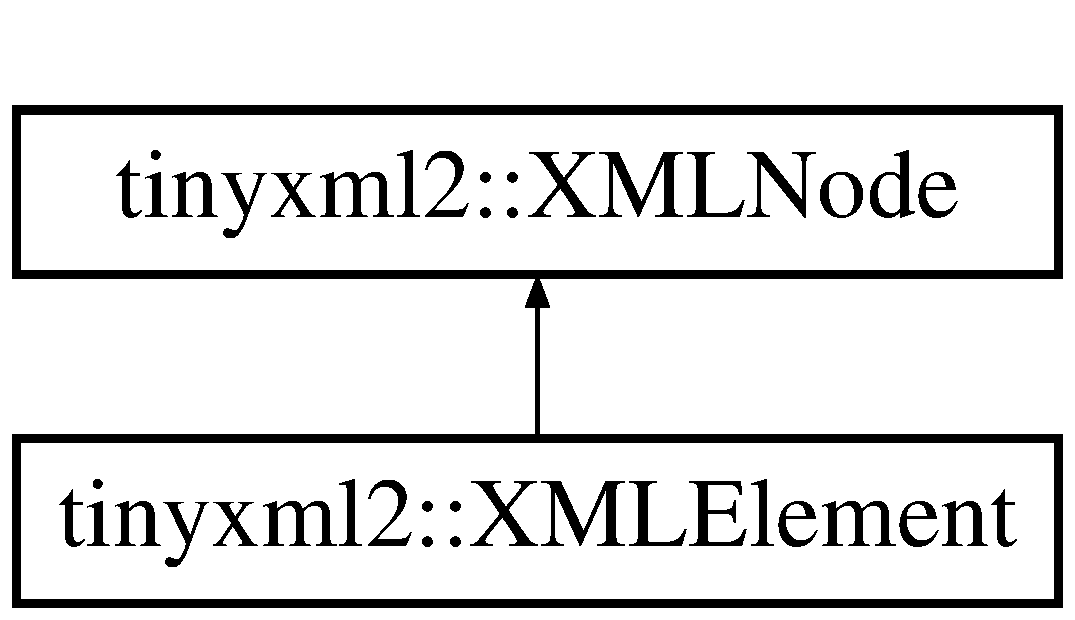
\includegraphics[height=2.000000cm]{classtinyxml2_1_1_x_m_l_element}
\end{center}
\end{figure}
\subsection*{Public Types}
\begin{DoxyCompactItemize}
\item 
enum \{ \hyperlink{classtinyxml2_1_1_x_m_l_element_a07a6ce25c17aaa505933db57f2373e50a78cf277c55b4655c86458dfecb11d349}{O\-P\-E\-N}, 
\hyperlink{classtinyxml2_1_1_x_m_l_element_a07a6ce25c17aaa505933db57f2373e50aa2f1f384020d2d4538ad2ec84930a028}{C\-L\-O\-S\-E\-D}, 
\hyperlink{classtinyxml2_1_1_x_m_l_element_a07a6ce25c17aaa505933db57f2373e50aa2857344b98a931536c443cd0cadc4b7}{C\-L\-O\-S\-I\-N\-G}
 \}
\end{DoxyCompactItemize}
\subsection*{Public Member Functions}
\begin{DoxyCompactItemize}
\item 
const char $\ast$ \hyperlink{classtinyxml2_1_1_x_m_l_element_a8bff355472bce2c60d4b50a212bf7f5f}{Name} () const 
\begin{DoxyCompactList}\small\item\em Get the name of an element (which is the \hyperlink{classtinyxml2_1_1_x_m_l_node_a7682be117e3b2b4ebfd517c1acaaadbf}{Value()} of the node.) \end{DoxyCompactList}\item 
void \hyperlink{classtinyxml2_1_1_x_m_l_element_a97712009a530d8cb8a63bf705f02b4f1}{Set\-Name} (const char $\ast$str, bool static\-Mem=false)
\begin{DoxyCompactList}\small\item\em Set the name of the element. \end{DoxyCompactList}\item 
virtual \hyperlink{classtinyxml2_1_1_x_m_l_element}{X\-M\-L\-Element} $\ast$ \hyperlink{classtinyxml2_1_1_x_m_l_element_ad9ff5c2dbc15df36cf664ce1b0ea0a5d}{To\-Element} ()
\begin{DoxyCompactList}\small\item\em Safely cast to an Element, or null. \end{DoxyCompactList}\item 
virtual const \hyperlink{classtinyxml2_1_1_x_m_l_element}{X\-M\-L\-Element} $\ast$ \hyperlink{classtinyxml2_1_1_x_m_l_element_a55acab615353ddabab48271f95816b0d}{To\-Element} () const 
\item 
virtual bool \hyperlink{classtinyxml2_1_1_x_m_l_element_a36d65438991a1e85096caf39ad13a099}{Accept} (\hyperlink{classtinyxml2_1_1_x_m_l_visitor}{X\-M\-L\-Visitor} $\ast$visitor) const 
\item 
const char $\ast$ \hyperlink{classtinyxml2_1_1_x_m_l_element_a7bdebdf1888074087237f3dd03912740}{Attribute} (const char $\ast$name, const char $\ast$value=0) const 
\item 
int \hyperlink{classtinyxml2_1_1_x_m_l_element_af86f05771c11a73a2896b662bb589ef5}{Int\-Attribute} (const char $\ast$name) const 
\item 
unsigned \hyperlink{classtinyxml2_1_1_x_m_l_element_aa5a41367b5118acec42a87f5f94cec2d}{Unsigned\-Attribute} (const char $\ast$name) const 
\begin{DoxyCompactList}\small\item\em See \hyperlink{classtinyxml2_1_1_x_m_l_element_af86f05771c11a73a2896b662bb589ef5}{Int\-Attribute()} \end{DoxyCompactList}\item 
bool \hyperlink{classtinyxml2_1_1_x_m_l_element_a34811e4d1881e4ecc95c49f0f3799115}{Bool\-Attribute} (const char $\ast$name) const 
\begin{DoxyCompactList}\small\item\em See \hyperlink{classtinyxml2_1_1_x_m_l_element_af86f05771c11a73a2896b662bb589ef5}{Int\-Attribute()} \end{DoxyCompactList}\item 
double \hyperlink{classtinyxml2_1_1_x_m_l_element_a536922a5cae9c9769a3dc1b7a8ff0d44}{Double\-Attribute} (const char $\ast$name) const 
\begin{DoxyCompactList}\small\item\em See \hyperlink{classtinyxml2_1_1_x_m_l_element_af86f05771c11a73a2896b662bb589ef5}{Int\-Attribute()} \end{DoxyCompactList}\item 
float \hyperlink{classtinyxml2_1_1_x_m_l_element_a33b69f123f995aff966d2e351bc51b1f}{Float\-Attribute} (const char $\ast$name) const 
\begin{DoxyCompactList}\small\item\em See \hyperlink{classtinyxml2_1_1_x_m_l_element_af86f05771c11a73a2896b662bb589ef5}{Int\-Attribute()} \end{DoxyCompactList}\item 
\hyperlink{namespacetinyxml2_a1fbf88509c3ac88c09117b1947414e08}{X\-M\-L\-Error} \hyperlink{classtinyxml2_1_1_x_m_l_element_a8b92c729346aa8ea9acd59ed3e9f2378}{Query\-Int\-Attribute} (const char $\ast$name, int $\ast$value) const 
\item 
\hyperlink{namespacetinyxml2_a1fbf88509c3ac88c09117b1947414e08}{X\-M\-L\-Error} \hyperlink{classtinyxml2_1_1_x_m_l_element_aa3d8d1b9311da8fc249b4352749aaa84}{Query\-Unsigned\-Attribute} (const char $\ast$name, unsigned int $\ast$value) const 
\begin{DoxyCompactList}\small\item\em See \hyperlink{classtinyxml2_1_1_x_m_l_element_a8b92c729346aa8ea9acd59ed3e9f2378}{Query\-Int\-Attribute()} \end{DoxyCompactList}\item 
\hyperlink{namespacetinyxml2_a1fbf88509c3ac88c09117b1947414e08}{X\-M\-L\-Error} \hyperlink{classtinyxml2_1_1_x_m_l_element_a2a58ee941c3cda23772c887a8f8b534e}{Query\-Bool\-Attribute} (const char $\ast$name, bool $\ast$value) const 
\begin{DoxyCompactList}\small\item\em See \hyperlink{classtinyxml2_1_1_x_m_l_element_a8b92c729346aa8ea9acd59ed3e9f2378}{Query\-Int\-Attribute()} \end{DoxyCompactList}\item 
\hyperlink{namespacetinyxml2_a1fbf88509c3ac88c09117b1947414e08}{X\-M\-L\-Error} \hyperlink{classtinyxml2_1_1_x_m_l_element_a1ffeed461d3e4020b39652cd6d3cd773}{Query\-Double\-Attribute} (const char $\ast$name, double $\ast$value) const 
\begin{DoxyCompactList}\small\item\em See \hyperlink{classtinyxml2_1_1_x_m_l_element_a8b92c729346aa8ea9acd59ed3e9f2378}{Query\-Int\-Attribute()} \end{DoxyCompactList}\item 
\hyperlink{namespacetinyxml2_a1fbf88509c3ac88c09117b1947414e08}{X\-M\-L\-Error} \hyperlink{classtinyxml2_1_1_x_m_l_element_a3f154e0b4b6903249ff9f758921758e5}{Query\-Float\-Attribute} (const char $\ast$name, float $\ast$value) const 
\begin{DoxyCompactList}\small\item\em See \hyperlink{classtinyxml2_1_1_x_m_l_element_a8b92c729346aa8ea9acd59ed3e9f2378}{Query\-Int\-Attribute()} \end{DoxyCompactList}\item 
int \hyperlink{classtinyxml2_1_1_x_m_l_element_aa471a199af9f137ef371f5db1ed1016b}{Query\-Attribute} (const char $\ast$name, int $\ast$value) const 
\item 
int \hyperlink{classtinyxml2_1_1_x_m_l_element_a60d18656aa70adb257eab18913aa4330}{Query\-Attribute} (const char $\ast$name, unsigned int $\ast$value) const 
\item 
int \hyperlink{classtinyxml2_1_1_x_m_l_element_a23fa8bac4250249c476c6bfdb6cb9b9c}{Query\-Attribute} (const char $\ast$name, bool $\ast$value) const 
\item 
int \hyperlink{classtinyxml2_1_1_x_m_l_element_a64aadcbf27423410e2896baf240f63f9}{Query\-Attribute} (const char $\ast$name, double $\ast$value) const 
\item 
int \hyperlink{classtinyxml2_1_1_x_m_l_element_afd553774be0e7760d73003058efa8df9}{Query\-Attribute} (const char $\ast$name, float $\ast$value) const 
\item 
void \hyperlink{classtinyxml2_1_1_x_m_l_element_a11943abf2d0831548c3790dd5d9f119c}{Set\-Attribute} (const char $\ast$name, const char $\ast$value)
\begin{DoxyCompactList}\small\item\em Sets the named attribute to value. \end{DoxyCompactList}\item 
void \hyperlink{classtinyxml2_1_1_x_m_l_element_aae6568c64c7f1cc88be8461ba41a79cf}{Set\-Attribute} (const char $\ast$name, int value)
\begin{DoxyCompactList}\small\item\em Sets the named attribute to value. \end{DoxyCompactList}\item 
void \hyperlink{classtinyxml2_1_1_x_m_l_element_ae143997e90064ba82326b29a9930ea8f}{Set\-Attribute} (const char $\ast$name, unsigned value)
\begin{DoxyCompactList}\small\item\em Sets the named attribute to value. \end{DoxyCompactList}\item 
void \hyperlink{classtinyxml2_1_1_x_m_l_element_aa848b696e6a75e4e545c6da9893b11e1}{Set\-Attribute} (const char $\ast$name, bool value)
\begin{DoxyCompactList}\small\item\em Sets the named attribute to value. \end{DoxyCompactList}\item 
void \hyperlink{classtinyxml2_1_1_x_m_l_element_a233397ee81e70eb5d4b814c5f8698533}{Set\-Attribute} (const char $\ast$name, double value)
\begin{DoxyCompactList}\small\item\em Sets the named attribute to value. \end{DoxyCompactList}\item 
void \hyperlink{classtinyxml2_1_1_x_m_l_element_aebd45aa7118964c30b32fe12e944628a}{Delete\-Attribute} (const char $\ast$name)
\item 
const \hyperlink{classtinyxml2_1_1_x_m_l_attribute}{X\-M\-L\-Attribute} $\ast$ \hyperlink{classtinyxml2_1_1_x_m_l_element_a67593e63558ffda0386699c3e4cc0b2c}{First\-Attribute} () const 
\begin{DoxyCompactList}\small\item\em Return the first attribute in the list. \end{DoxyCompactList}\item 
const \hyperlink{classtinyxml2_1_1_x_m_l_attribute}{X\-M\-L\-Attribute} $\ast$ \hyperlink{classtinyxml2_1_1_x_m_l_element_aaf46b0799ea419e5d070ac9a357de48f}{Find\-Attribute} (const char $\ast$name) const 
\begin{DoxyCompactList}\small\item\em Query a specific attribute in the list. \end{DoxyCompactList}\item 
const char $\ast$ \hyperlink{classtinyxml2_1_1_x_m_l_element_a56cc727044dad002b978256754d43a4b}{Get\-Text} () const 
\item 
\hyperlink{namespacetinyxml2_a1fbf88509c3ac88c09117b1947414e08}{X\-M\-L\-Error} \hyperlink{classtinyxml2_1_1_x_m_l_element_a71327c9a9d8840562bd204f46d0a7189}{Query\-Int\-Text} (int $\ast$ival) const 
\item 
\hyperlink{namespacetinyxml2_a1fbf88509c3ac88c09117b1947414e08}{X\-M\-L\-Error} \hyperlink{classtinyxml2_1_1_x_m_l_element_a2192091dec0c06be8b14f4e912c01758}{Query\-Unsigned\-Text} (unsigned $\ast$uval) const 
\begin{DoxyCompactList}\small\item\em See \hyperlink{classtinyxml2_1_1_x_m_l_element_a71327c9a9d8840562bd204f46d0a7189}{Query\-Int\-Text()} \end{DoxyCompactList}\item 
\hyperlink{namespacetinyxml2_a1fbf88509c3ac88c09117b1947414e08}{X\-M\-L\-Error} \hyperlink{classtinyxml2_1_1_x_m_l_element_afeb060672fa934163fc573e692b7fe38}{Query\-Bool\-Text} (bool $\ast$bval) const 
\begin{DoxyCompactList}\small\item\em See \hyperlink{classtinyxml2_1_1_x_m_l_element_a71327c9a9d8840562bd204f46d0a7189}{Query\-Int\-Text()} \end{DoxyCompactList}\item 
\hyperlink{namespacetinyxml2_a1fbf88509c3ac88c09117b1947414e08}{X\-M\-L\-Error} \hyperlink{classtinyxml2_1_1_x_m_l_element_aad931c42548907dbea416f7365d78b57}{Query\-Double\-Text} (double $\ast$dval) const 
\begin{DoxyCompactList}\small\item\em See \hyperlink{classtinyxml2_1_1_x_m_l_element_a71327c9a9d8840562bd204f46d0a7189}{Query\-Int\-Text()} \end{DoxyCompactList}\item 
\hyperlink{namespacetinyxml2_a1fbf88509c3ac88c09117b1947414e08}{X\-M\-L\-Error} \hyperlink{classtinyxml2_1_1_x_m_l_element_a11fa26e1dbca88e973964c1d9b597658}{Query\-Float\-Text} (float $\ast$fval) const 
\begin{DoxyCompactList}\small\item\em See \hyperlink{classtinyxml2_1_1_x_m_l_element_a71327c9a9d8840562bd204f46d0a7189}{Query\-Int\-Text()} \end{DoxyCompactList}\item 
int \hyperlink{classtinyxml2_1_1_x_m_l_element_a2e3d9f938307a05963d7c4b8cd55754e}{Closing\-Type} () const 
\item 
char $\ast$ \hyperlink{classtinyxml2_1_1_x_m_l_element_aaafdd2a5618abe80a2c1839ad3ccd492}{Parse\-Deep} (char $\ast$p, \hyperlink{classtinyxml2_1_1_str_pair}{Str\-Pair} $\ast$end\-Tag)
\item 
virtual \hyperlink{classtinyxml2_1_1_x_m_l_node}{X\-M\-L\-Node} $\ast$ \hyperlink{classtinyxml2_1_1_x_m_l_element_a85d85e32c18863fff1eeed53ae1ce23d}{Shallow\-Clone} (\hyperlink{classtinyxml2_1_1_x_m_l_document}{X\-M\-L\-Document} $\ast$document) const 
\item 
virtual bool \hyperlink{classtinyxml2_1_1_x_m_l_element_a25d51a2aad92625c78441457d58c85bc}{Shallow\-Equal} (const \hyperlink{classtinyxml2_1_1_x_m_l_node}{X\-M\-L\-Node} $\ast$compare) const 
\end{DoxyCompactItemize}
\subsection*{Friends}
\begin{DoxyCompactItemize}
\item 
class \hyperlink{classtinyxml2_1_1_x_m_l_element_a449202cfc89e7ae5c2f81995476f9ec1}{X\-M\-L\-Base}
\item 
class \hyperlink{classtinyxml2_1_1_x_m_l_element_a4eee3bda60c60a30e4e8cd4ea91c4c6e}{X\-M\-L\-Document}
\end{DoxyCompactItemize}
\subsection*{Additional Inherited Members}


\subsection{Detailed Description}
The element is a container class. It has a value, the element name, and can contain other elements, text, comments, and unknowns. Elements also contain an arbitrary number of attributes. 

Definition at line 1108 of file tinyxml2.\-hpp.



\subsection{Member Enumeration Documentation}
\hypertarget{classtinyxml2_1_1_x_m_l_element_a07a6ce25c17aaa505933db57f2373e50}{\subsubsection[{anonymous enum}]{\setlength{\rightskip}{0pt plus 5cm}anonymous enum}}\label{classtinyxml2_1_1_x_m_l_element_a07a6ce25c17aaa505933db57f2373e50}
\begin{Desc}
\item[Enumerator]\par
\begin{description}
\index{O\-P\-E\-N@{O\-P\-E\-N}!tinyxml2\-::\-X\-M\-L\-Element@{tinyxml2\-::\-X\-M\-L\-Element}}\index{tinyxml2\-::\-X\-M\-L\-Element@{tinyxml2\-::\-X\-M\-L\-Element}!O\-P\-E\-N@{O\-P\-E\-N}}\item[{\em 
\hypertarget{classtinyxml2_1_1_x_m_l_element_a07a6ce25c17aaa505933db57f2373e50a78cf277c55b4655c86458dfecb11d349}{O\-P\-E\-N}\label{classtinyxml2_1_1_x_m_l_element_a07a6ce25c17aaa505933db57f2373e50a78cf277c55b4655c86458dfecb11d349}
}]\index{C\-L\-O\-S\-E\-D@{C\-L\-O\-S\-E\-D}!tinyxml2\-::\-X\-M\-L\-Element@{tinyxml2\-::\-X\-M\-L\-Element}}\index{tinyxml2\-::\-X\-M\-L\-Element@{tinyxml2\-::\-X\-M\-L\-Element}!C\-L\-O\-S\-E\-D@{C\-L\-O\-S\-E\-D}}\item[{\em 
\hypertarget{classtinyxml2_1_1_x_m_l_element_a07a6ce25c17aaa505933db57f2373e50aa2f1f384020d2d4538ad2ec84930a028}{C\-L\-O\-S\-E\-D}\label{classtinyxml2_1_1_x_m_l_element_a07a6ce25c17aaa505933db57f2373e50aa2f1f384020d2d4538ad2ec84930a028}
}]\index{C\-L\-O\-S\-I\-N\-G@{C\-L\-O\-S\-I\-N\-G}!tinyxml2\-::\-X\-M\-L\-Element@{tinyxml2\-::\-X\-M\-L\-Element}}\index{tinyxml2\-::\-X\-M\-L\-Element@{tinyxml2\-::\-X\-M\-L\-Element}!C\-L\-O\-S\-I\-N\-G@{C\-L\-O\-S\-I\-N\-G}}\item[{\em 
\hypertarget{classtinyxml2_1_1_x_m_l_element_a07a6ce25c17aaa505933db57f2373e50aa2857344b98a931536c443cd0cadc4b7}{C\-L\-O\-S\-I\-N\-G}\label{classtinyxml2_1_1_x_m_l_element_a07a6ce25c17aaa505933db57f2373e50aa2857344b98a931536c443cd0cadc4b7}
}]\end{description}
\end{Desc}


Definition at line 1386 of file tinyxml2.\-hpp.



\subsection{Member Function Documentation}
\hypertarget{classtinyxml2_1_1_x_m_l_element_a36d65438991a1e85096caf39ad13a099}{\index{tinyxml2\-::\-X\-M\-L\-Element@{tinyxml2\-::\-X\-M\-L\-Element}!Accept@{Accept}}
\index{Accept@{Accept}!tinyxml2::XMLElement@{tinyxml2\-::\-X\-M\-L\-Element}}
\subsubsection[{Accept}]{\setlength{\rightskip}{0pt plus 5cm}bool tinyxml2\-::\-X\-M\-L\-Element\-::\-Accept (
\begin{DoxyParamCaption}
\item[{{\bf X\-M\-L\-Visitor} $\ast$}]{visitor}
\end{DoxyParamCaption}
) const\hspace{0.3cm}{\ttfamily [virtual]}}}\label{classtinyxml2_1_1_x_m_l_element_a36d65438991a1e85096caf39ad13a099}
Accept a hierarchical visit of the nodes in the Tiny\-X\-M\-L-\/2 D\-O\-M. Every node in the \hyperlink{namespace_x_m_l}{X\-M\-L} tree will be conditionally visited and the host will be called back via the \hyperlink{classtinyxml2_1_1_x_m_l_visitor}{X\-M\-L\-Visitor} interface.

This is essentially a S\-A\-X interface for Tiny\-X\-M\-L-\/2. (Note however it doesn't re-\/parse the \hyperlink{namespace_x_m_l}{X\-M\-L} for the callbacks, so the performance of Tiny\-X\-M\-L-\/2 is unchanged by using this interface versus any other.)

The interface has been based on ideas from\-:


\begin{DoxyItemize}
\item \href{http://www.saxproject.org/}{\tt http\-://www.\-saxproject.\-org/}
\item \href{http://c2.com/cgi/wiki?HierarchicalVisitorPattern}{\tt http\-://c2.\-com/cgi/wiki?\-Hierarchical\-Visitor\-Pattern}
\end{DoxyItemize}

Which are both good references for \char`\"{}visiting\char`\"{}.

An example of using \hyperlink{classtinyxml2_1_1_x_m_l_element_a36d65438991a1e85096caf39ad13a099}{Accept()}\-: \begin{DoxyVerb}XMLPrinter printer;
tinyxmlDoc.Accept( &printer );
const char* xmlcstr = printer.CStr();
\end{DoxyVerb}
 

Implements \hyperlink{classtinyxml2_1_1_x_m_l_node_a81e66df0a44c67a7af17f3b77a152785}{tinyxml2\-::\-X\-M\-L\-Node}.



Definition at line 1473 of file tinyxml2.\-cpp.

\hypertarget{classtinyxml2_1_1_x_m_l_element_a7bdebdf1888074087237f3dd03912740}{\index{tinyxml2\-::\-X\-M\-L\-Element@{tinyxml2\-::\-X\-M\-L\-Element}!Attribute@{Attribute}}
\index{Attribute@{Attribute}!tinyxml2::XMLElement@{tinyxml2\-::\-X\-M\-L\-Element}}
\subsubsection[{Attribute}]{\setlength{\rightskip}{0pt plus 5cm}const char $\ast$ tinyxml2\-::\-X\-M\-L\-Element\-::\-Attribute (
\begin{DoxyParamCaption}
\item[{const char $\ast$}]{name, }
\item[{const char $\ast$}]{value = {\ttfamily 0}}
\end{DoxyParamCaption}
) const}}\label{classtinyxml2_1_1_x_m_l_element_a7bdebdf1888074087237f3dd03912740}
Given an attribute name, \hyperlink{classtinyxml2_1_1_x_m_l_element_a7bdebdf1888074087237f3dd03912740}{Attribute()} returns the value for the attribute of that name, or null if none exists. For example\-:

\begin{DoxyVerb}const char* value = ele->Attribute( "foo" );
\end{DoxyVerb}


The 'value' parameter is normally null. However, if specified, the attribute will only be returned if the 'name' and 'value' match. This allow you to write code\-:

\begin{DoxyVerb}if ( ele->Attribute( "foo", "bar" ) ) callFooIsBar();
\end{DoxyVerb}


rather than\-: \begin{DoxyVerb}if ( ele->Attribute( "foo" ) ) {
    if ( strcmp( ele->Attribute( "foo" ), "bar" ) == 0 ) callFooIsBar();
}
\end{DoxyVerb}
 

Definition at line 1208 of file tinyxml2.\-cpp.

\hypertarget{classtinyxml2_1_1_x_m_l_element_a34811e4d1881e4ecc95c49f0f3799115}{\index{tinyxml2\-::\-X\-M\-L\-Element@{tinyxml2\-::\-X\-M\-L\-Element}!Bool\-Attribute@{Bool\-Attribute}}
\index{Bool\-Attribute@{Bool\-Attribute}!tinyxml2::XMLElement@{tinyxml2\-::\-X\-M\-L\-Element}}
\subsubsection[{Bool\-Attribute}]{\setlength{\rightskip}{0pt plus 5cm}bool tinyxml2\-::\-X\-M\-L\-Element\-::\-Bool\-Attribute (
\begin{DoxyParamCaption}
\item[{const char $\ast$}]{name}
\end{DoxyParamCaption}
) const\hspace{0.3cm}{\ttfamily [inline]}}}\label{classtinyxml2_1_1_x_m_l_element_a34811e4d1881e4ecc95c49f0f3799115}


See \hyperlink{classtinyxml2_1_1_x_m_l_element_af86f05771c11a73a2896b662bb589ef5}{Int\-Attribute()} 



Definition at line 1172 of file tinyxml2.\-hpp.

\hypertarget{classtinyxml2_1_1_x_m_l_element_a2e3d9f938307a05963d7c4b8cd55754e}{\index{tinyxml2\-::\-X\-M\-L\-Element@{tinyxml2\-::\-X\-M\-L\-Element}!Closing\-Type@{Closing\-Type}}
\index{Closing\-Type@{Closing\-Type}!tinyxml2::XMLElement@{tinyxml2\-::\-X\-M\-L\-Element}}
\subsubsection[{Closing\-Type}]{\setlength{\rightskip}{0pt plus 5cm}int tinyxml2\-::\-X\-M\-L\-Element\-::\-Closing\-Type (
\begin{DoxyParamCaption}
{}
\end{DoxyParamCaption}
) const\hspace{0.3cm}{\ttfamily [inline]}}}\label{classtinyxml2_1_1_x_m_l_element_a2e3d9f938307a05963d7c4b8cd55754e}


Definition at line 1391 of file tinyxml2.\-hpp.

\hypertarget{classtinyxml2_1_1_x_m_l_element_aebd45aa7118964c30b32fe12e944628a}{\index{tinyxml2\-::\-X\-M\-L\-Element@{tinyxml2\-::\-X\-M\-L\-Element}!Delete\-Attribute@{Delete\-Attribute}}
\index{Delete\-Attribute@{Delete\-Attribute}!tinyxml2::XMLElement@{tinyxml2\-::\-X\-M\-L\-Element}}
\subsubsection[{Delete\-Attribute}]{\setlength{\rightskip}{0pt plus 5cm}void tinyxml2\-::\-X\-M\-L\-Element\-::\-Delete\-Attribute (
\begin{DoxyParamCaption}
\item[{const char $\ast$}]{name}
\end{DoxyParamCaption}
)}}\label{classtinyxml2_1_1_x_m_l_element_aebd45aa7118964c30b32fe12e944628a}
Delete an attribute. 

Definition at line 1323 of file tinyxml2.\-cpp.

\hypertarget{classtinyxml2_1_1_x_m_l_element_a536922a5cae9c9769a3dc1b7a8ff0d44}{\index{tinyxml2\-::\-X\-M\-L\-Element@{tinyxml2\-::\-X\-M\-L\-Element}!Double\-Attribute@{Double\-Attribute}}
\index{Double\-Attribute@{Double\-Attribute}!tinyxml2::XMLElement@{tinyxml2\-::\-X\-M\-L\-Element}}
\subsubsection[{Double\-Attribute}]{\setlength{\rightskip}{0pt plus 5cm}double tinyxml2\-::\-X\-M\-L\-Element\-::\-Double\-Attribute (
\begin{DoxyParamCaption}
\item[{const char $\ast$}]{name}
\end{DoxyParamCaption}
) const\hspace{0.3cm}{\ttfamily [inline]}}}\label{classtinyxml2_1_1_x_m_l_element_a536922a5cae9c9769a3dc1b7a8ff0d44}


See \hyperlink{classtinyxml2_1_1_x_m_l_element_af86f05771c11a73a2896b662bb589ef5}{Int\-Attribute()} 



Definition at line 1178 of file tinyxml2.\-hpp.

\hypertarget{classtinyxml2_1_1_x_m_l_element_aaf46b0799ea419e5d070ac9a357de48f}{\index{tinyxml2\-::\-X\-M\-L\-Element@{tinyxml2\-::\-X\-M\-L\-Element}!Find\-Attribute@{Find\-Attribute}}
\index{Find\-Attribute@{Find\-Attribute}!tinyxml2::XMLElement@{tinyxml2\-::\-X\-M\-L\-Element}}
\subsubsection[{Find\-Attribute}]{\setlength{\rightskip}{0pt plus 5cm}const {\bf X\-M\-L\-Attribute} $\ast$ tinyxml2\-::\-X\-M\-L\-Element\-::\-Find\-Attribute (
\begin{DoxyParamCaption}
\item[{const char $\ast$}]{name}
\end{DoxyParamCaption}
) const}}\label{classtinyxml2_1_1_x_m_l_element_aaf46b0799ea419e5d070ac9a357de48f}


Query a specific attribute in the list. 



Definition at line 1196 of file tinyxml2.\-cpp.

\hypertarget{classtinyxml2_1_1_x_m_l_element_a67593e63558ffda0386699c3e4cc0b2c}{\index{tinyxml2\-::\-X\-M\-L\-Element@{tinyxml2\-::\-X\-M\-L\-Element}!First\-Attribute@{First\-Attribute}}
\index{First\-Attribute@{First\-Attribute}!tinyxml2::XMLElement@{tinyxml2\-::\-X\-M\-L\-Element}}
\subsubsection[{First\-Attribute}]{\setlength{\rightskip}{0pt plus 5cm}const {\bf X\-M\-L\-Attribute}$\ast$ tinyxml2\-::\-X\-M\-L\-Element\-::\-First\-Attribute (
\begin{DoxyParamCaption}
{}
\end{DoxyParamCaption}
) const\hspace{0.3cm}{\ttfamily [inline]}}}\label{classtinyxml2_1_1_x_m_l_element_a67593e63558ffda0386699c3e4cc0b2c}


Return the first attribute in the list. 



Definition at line 1313 of file tinyxml2.\-hpp.

\hypertarget{classtinyxml2_1_1_x_m_l_element_a33b69f123f995aff966d2e351bc51b1f}{\index{tinyxml2\-::\-X\-M\-L\-Element@{tinyxml2\-::\-X\-M\-L\-Element}!Float\-Attribute@{Float\-Attribute}}
\index{Float\-Attribute@{Float\-Attribute}!tinyxml2::XMLElement@{tinyxml2\-::\-X\-M\-L\-Element}}
\subsubsection[{Float\-Attribute}]{\setlength{\rightskip}{0pt plus 5cm}float tinyxml2\-::\-X\-M\-L\-Element\-::\-Float\-Attribute (
\begin{DoxyParamCaption}
\item[{const char $\ast$}]{name}
\end{DoxyParamCaption}
) const\hspace{0.3cm}{\ttfamily [inline]}}}\label{classtinyxml2_1_1_x_m_l_element_a33b69f123f995aff966d2e351bc51b1f}


See \hyperlink{classtinyxml2_1_1_x_m_l_element_af86f05771c11a73a2896b662bb589ef5}{Int\-Attribute()} 



Definition at line 1184 of file tinyxml2.\-hpp.

\hypertarget{classtinyxml2_1_1_x_m_l_element_a56cc727044dad002b978256754d43a4b}{\index{tinyxml2\-::\-X\-M\-L\-Element@{tinyxml2\-::\-X\-M\-L\-Element}!Get\-Text@{Get\-Text}}
\index{Get\-Text@{Get\-Text}!tinyxml2::XMLElement@{tinyxml2\-::\-X\-M\-L\-Element}}
\subsubsection[{Get\-Text}]{\setlength{\rightskip}{0pt plus 5cm}const char $\ast$ tinyxml2\-::\-X\-M\-L\-Element\-::\-Get\-Text (
\begin{DoxyParamCaption}
{}
\end{DoxyParamCaption}
) const}}\label{classtinyxml2_1_1_x_m_l_element_a56cc727044dad002b978256754d43a4b}
Convenience function for easy access to the text inside an element. Although easy and concise, \hyperlink{classtinyxml2_1_1_x_m_l_element_a56cc727044dad002b978256754d43a4b}{Get\-Text()} is limited compared to getting the \hyperlink{classtinyxml2_1_1_x_m_l_text}{X\-M\-L\-Text} child and accessing it directly.

If the first child of 'this' is a \hyperlink{classtinyxml2_1_1_x_m_l_text}{X\-M\-L\-Text}, the \hyperlink{classtinyxml2_1_1_x_m_l_element_a56cc727044dad002b978256754d43a4b}{Get\-Text()} returns the character string of the Text node, else null is returned.

This is a convenient method for getting the text of simple contained text\-: \begin{DoxyVerb}<foo>This is text</foo>
    const char* str = fooElement->GetText();
\end{DoxyVerb}


'str' will be a pointer to \char`\"{}\-This is text\char`\"{}.

Note that this function can be misleading. If the element foo was created from this \hyperlink{namespace_x_m_l}{X\-M\-L}\-: \begin{DoxyVerb}    <foo><b>This is text</b></foo>
\end{DoxyVerb}


then the value of str would be null. The first child node isn't a text node, it is another element. From this \hyperlink{namespace_x_m_l}{X\-M\-L}\-: \begin{DoxyVerb}    <foo>This is <b>text</b></foo>
\end{DoxyVerb}
 \hyperlink{classtinyxml2_1_1_x_m_l_element_a56cc727044dad002b978256754d43a4b}{Get\-Text()} will return \char`\"{}\-This is \char`\"{}. 

Definition at line 1221 of file tinyxml2.\-cpp.

\hypertarget{classtinyxml2_1_1_x_m_l_element_af86f05771c11a73a2896b662bb589ef5}{\index{tinyxml2\-::\-X\-M\-L\-Element@{tinyxml2\-::\-X\-M\-L\-Element}!Int\-Attribute@{Int\-Attribute}}
\index{Int\-Attribute@{Int\-Attribute}!tinyxml2::XMLElement@{tinyxml2\-::\-X\-M\-L\-Element}}
\subsubsection[{Int\-Attribute}]{\setlength{\rightskip}{0pt plus 5cm}int tinyxml2\-::\-X\-M\-L\-Element\-::\-Int\-Attribute (
\begin{DoxyParamCaption}
\item[{const char $\ast$}]{name}
\end{DoxyParamCaption}
) const\hspace{0.3cm}{\ttfamily [inline]}}}\label{classtinyxml2_1_1_x_m_l_element_af86f05771c11a73a2896b662bb589ef5}
Given an attribute name, \hyperlink{classtinyxml2_1_1_x_m_l_element_af86f05771c11a73a2896b662bb589ef5}{Int\-Attribute()} returns the value of the attribute interpreted as an integer. 0 will be returned if there is an error. For a method with error checking, see \hyperlink{classtinyxml2_1_1_x_m_l_element_a8b92c729346aa8ea9acd59ed3e9f2378}{Query\-Int\-Attribute()} 

Definition at line 1160 of file tinyxml2.\-hpp.

\hypertarget{classtinyxml2_1_1_x_m_l_element_a8bff355472bce2c60d4b50a212bf7f5f}{\index{tinyxml2\-::\-X\-M\-L\-Element@{tinyxml2\-::\-X\-M\-L\-Element}!Name@{Name}}
\index{Name@{Name}!tinyxml2::XMLElement@{tinyxml2\-::\-X\-M\-L\-Element}}
\subsubsection[{Name}]{\setlength{\rightskip}{0pt plus 5cm}const char$\ast$ tinyxml2\-::\-X\-M\-L\-Element\-::\-Name (
\begin{DoxyParamCaption}
{}
\end{DoxyParamCaption}
) const\hspace{0.3cm}{\ttfamily [inline]}}}\label{classtinyxml2_1_1_x_m_l_element_a8bff355472bce2c60d4b50a212bf7f5f}


Get the name of an element (which is the \hyperlink{classtinyxml2_1_1_x_m_l_node_a7682be117e3b2b4ebfd517c1acaaadbf}{Value()} of the node.) 



Definition at line 1114 of file tinyxml2.\-hpp.

\hypertarget{classtinyxml2_1_1_x_m_l_element_aaafdd2a5618abe80a2c1839ad3ccd492}{\index{tinyxml2\-::\-X\-M\-L\-Element@{tinyxml2\-::\-X\-M\-L\-Element}!Parse\-Deep@{Parse\-Deep}}
\index{Parse\-Deep@{Parse\-Deep}!tinyxml2::XMLElement@{tinyxml2\-::\-X\-M\-L\-Element}}
\subsubsection[{Parse\-Deep}]{\setlength{\rightskip}{0pt plus 5cm}char $\ast$ tinyxml2\-::\-X\-M\-L\-Element\-::\-Parse\-Deep (
\begin{DoxyParamCaption}
\item[{char $\ast$}]{p, }
\item[{{\bf Str\-Pair} $\ast$}]{end\-Tag}
\end{DoxyParamCaption}
)\hspace{0.3cm}{\ttfamily [virtual]}}}\label{classtinyxml2_1_1_x_m_l_element_aaafdd2a5618abe80a2c1839ad3ccd492}


Reimplemented from \hyperlink{classtinyxml2_1_1_x_m_l_node_a7610d0f603e8b603d2078521811a23c1}{tinyxml2\-::\-X\-M\-L\-Node}.



Definition at line 1403 of file tinyxml2.\-cpp.

\hypertarget{classtinyxml2_1_1_x_m_l_element_aa471a199af9f137ef371f5db1ed1016b}{\index{tinyxml2\-::\-X\-M\-L\-Element@{tinyxml2\-::\-X\-M\-L\-Element}!Query\-Attribute@{Query\-Attribute}}
\index{Query\-Attribute@{Query\-Attribute}!tinyxml2::XMLElement@{tinyxml2\-::\-X\-M\-L\-Element}}
\subsubsection[{Query\-Attribute}]{\setlength{\rightskip}{0pt plus 5cm}int tinyxml2\-::\-X\-M\-L\-Element\-::\-Query\-Attribute (
\begin{DoxyParamCaption}
\item[{const char $\ast$}]{name, }
\item[{int $\ast$}]{value}
\end{DoxyParamCaption}
) const\hspace{0.3cm}{\ttfamily [inline]}}}\label{classtinyxml2_1_1_x_m_l_element_aa471a199af9f137ef371f5db1ed1016b}
Given an attribute name, \hyperlink{classtinyxml2_1_1_x_m_l_element_aa471a199af9f137ef371f5db1ed1016b}{Query\-Attribute()} returns X\-M\-L\-\_\-\-N\-O\-\_\-\-E\-R\-R\-O\-R, X\-M\-L\-\_\-\-W\-R\-O\-N\-G\-\_\-\-A\-T\-T\-R\-I\-B\-U\-T\-E\-\_\-\-T\-Y\-P\-E if the conversion can't be performed, or X\-M\-L\-\_\-\-N\-O\-\_\-\-A\-T\-T\-R\-I\-B\-U\-T\-E if the attribute doesn't exist. It is overloaded for the primitive types, and is a generally more convenient replacement of \hyperlink{classtinyxml2_1_1_x_m_l_element_a8b92c729346aa8ea9acd59ed3e9f2378}{Query\-Int\-Attribute()} and related functions.

If successful, the result of the conversion will be written to 'value'. If not successful, nothing will be written to 'value'. This allows you to provide default value\-:

\begin{DoxyVerb}int value = 10;
QueryAttribute( "foo", &value );        // if "foo" isn't found, value will still be 10
\end{DoxyVerb}
 

Definition at line 1261 of file tinyxml2.\-hpp.

\hypertarget{classtinyxml2_1_1_x_m_l_element_a60d18656aa70adb257eab18913aa4330}{\index{tinyxml2\-::\-X\-M\-L\-Element@{tinyxml2\-::\-X\-M\-L\-Element}!Query\-Attribute@{Query\-Attribute}}
\index{Query\-Attribute@{Query\-Attribute}!tinyxml2::XMLElement@{tinyxml2\-::\-X\-M\-L\-Element}}
\subsubsection[{Query\-Attribute}]{\setlength{\rightskip}{0pt plus 5cm}int tinyxml2\-::\-X\-M\-L\-Element\-::\-Query\-Attribute (
\begin{DoxyParamCaption}
\item[{const char $\ast$}]{name, }
\item[{unsigned int $\ast$}]{value}
\end{DoxyParamCaption}
) const\hspace{0.3cm}{\ttfamily [inline]}}}\label{classtinyxml2_1_1_x_m_l_element_a60d18656aa70adb257eab18913aa4330}


Definition at line 1265 of file tinyxml2.\-hpp.

\hypertarget{classtinyxml2_1_1_x_m_l_element_a23fa8bac4250249c476c6bfdb6cb9b9c}{\index{tinyxml2\-::\-X\-M\-L\-Element@{tinyxml2\-::\-X\-M\-L\-Element}!Query\-Attribute@{Query\-Attribute}}
\index{Query\-Attribute@{Query\-Attribute}!tinyxml2::XMLElement@{tinyxml2\-::\-X\-M\-L\-Element}}
\subsubsection[{Query\-Attribute}]{\setlength{\rightskip}{0pt plus 5cm}int tinyxml2\-::\-X\-M\-L\-Element\-::\-Query\-Attribute (
\begin{DoxyParamCaption}
\item[{const char $\ast$}]{name, }
\item[{bool $\ast$}]{value}
\end{DoxyParamCaption}
) const\hspace{0.3cm}{\ttfamily [inline]}}}\label{classtinyxml2_1_1_x_m_l_element_a23fa8bac4250249c476c6bfdb6cb9b9c}


Definition at line 1269 of file tinyxml2.\-hpp.

\hypertarget{classtinyxml2_1_1_x_m_l_element_a64aadcbf27423410e2896baf240f63f9}{\index{tinyxml2\-::\-X\-M\-L\-Element@{tinyxml2\-::\-X\-M\-L\-Element}!Query\-Attribute@{Query\-Attribute}}
\index{Query\-Attribute@{Query\-Attribute}!tinyxml2::XMLElement@{tinyxml2\-::\-X\-M\-L\-Element}}
\subsubsection[{Query\-Attribute}]{\setlength{\rightskip}{0pt plus 5cm}int tinyxml2\-::\-X\-M\-L\-Element\-::\-Query\-Attribute (
\begin{DoxyParamCaption}
\item[{const char $\ast$}]{name, }
\item[{double $\ast$}]{value}
\end{DoxyParamCaption}
) const\hspace{0.3cm}{\ttfamily [inline]}}}\label{classtinyxml2_1_1_x_m_l_element_a64aadcbf27423410e2896baf240f63f9}


Definition at line 1273 of file tinyxml2.\-hpp.

\hypertarget{classtinyxml2_1_1_x_m_l_element_afd553774be0e7760d73003058efa8df9}{\index{tinyxml2\-::\-X\-M\-L\-Element@{tinyxml2\-::\-X\-M\-L\-Element}!Query\-Attribute@{Query\-Attribute}}
\index{Query\-Attribute@{Query\-Attribute}!tinyxml2::XMLElement@{tinyxml2\-::\-X\-M\-L\-Element}}
\subsubsection[{Query\-Attribute}]{\setlength{\rightskip}{0pt plus 5cm}int tinyxml2\-::\-X\-M\-L\-Element\-::\-Query\-Attribute (
\begin{DoxyParamCaption}
\item[{const char $\ast$}]{name, }
\item[{float $\ast$}]{value}
\end{DoxyParamCaption}
) const\hspace{0.3cm}{\ttfamily [inline]}}}\label{classtinyxml2_1_1_x_m_l_element_afd553774be0e7760d73003058efa8df9}


Definition at line 1277 of file tinyxml2.\-hpp.

\hypertarget{classtinyxml2_1_1_x_m_l_element_a2a58ee941c3cda23772c887a8f8b534e}{\index{tinyxml2\-::\-X\-M\-L\-Element@{tinyxml2\-::\-X\-M\-L\-Element}!Query\-Bool\-Attribute@{Query\-Bool\-Attribute}}
\index{Query\-Bool\-Attribute@{Query\-Bool\-Attribute}!tinyxml2::XMLElement@{tinyxml2\-::\-X\-M\-L\-Element}}
\subsubsection[{Query\-Bool\-Attribute}]{\setlength{\rightskip}{0pt plus 5cm}{\bf X\-M\-L\-Error} tinyxml2\-::\-X\-M\-L\-Element\-::\-Query\-Bool\-Attribute (
\begin{DoxyParamCaption}
\item[{const char $\ast$}]{name, }
\item[{bool $\ast$}]{value}
\end{DoxyParamCaption}
) const\hspace{0.3cm}{\ttfamily [inline]}}}\label{classtinyxml2_1_1_x_m_l_element_a2a58ee941c3cda23772c887a8f8b534e}


See \hyperlink{classtinyxml2_1_1_x_m_l_element_a8b92c729346aa8ea9acd59ed3e9f2378}{Query\-Int\-Attribute()} 



Definition at line 1219 of file tinyxml2.\-hpp.

\hypertarget{classtinyxml2_1_1_x_m_l_element_afeb060672fa934163fc573e692b7fe38}{\index{tinyxml2\-::\-X\-M\-L\-Element@{tinyxml2\-::\-X\-M\-L\-Element}!Query\-Bool\-Text@{Query\-Bool\-Text}}
\index{Query\-Bool\-Text@{Query\-Bool\-Text}!tinyxml2::XMLElement@{tinyxml2\-::\-X\-M\-L\-Element}}
\subsubsection[{Query\-Bool\-Text}]{\setlength{\rightskip}{0pt plus 5cm}{\bf X\-M\-L\-Error} tinyxml2\-::\-X\-M\-L\-Element\-::\-Query\-Bool\-Text (
\begin{DoxyParamCaption}
\item[{bool $\ast$}]{bval}
\end{DoxyParamCaption}
) const}}\label{classtinyxml2_1_1_x_m_l_element_afeb060672fa934163fc573e692b7fe38}


See \hyperlink{classtinyxml2_1_1_x_m_l_element_a71327c9a9d8840562bd204f46d0a7189}{Query\-Int\-Text()} 



Definition at line 1256 of file tinyxml2.\-cpp.

\hypertarget{classtinyxml2_1_1_x_m_l_element_a1ffeed461d3e4020b39652cd6d3cd773}{\index{tinyxml2\-::\-X\-M\-L\-Element@{tinyxml2\-::\-X\-M\-L\-Element}!Query\-Double\-Attribute@{Query\-Double\-Attribute}}
\index{Query\-Double\-Attribute@{Query\-Double\-Attribute}!tinyxml2::XMLElement@{tinyxml2\-::\-X\-M\-L\-Element}}
\subsubsection[{Query\-Double\-Attribute}]{\setlength{\rightskip}{0pt plus 5cm}{\bf X\-M\-L\-Error} tinyxml2\-::\-X\-M\-L\-Element\-::\-Query\-Double\-Attribute (
\begin{DoxyParamCaption}
\item[{const char $\ast$}]{name, }
\item[{double $\ast$}]{value}
\end{DoxyParamCaption}
) const\hspace{0.3cm}{\ttfamily [inline]}}}\label{classtinyxml2_1_1_x_m_l_element_a1ffeed461d3e4020b39652cd6d3cd773}


See \hyperlink{classtinyxml2_1_1_x_m_l_element_a8b92c729346aa8ea9acd59ed3e9f2378}{Query\-Int\-Attribute()} 



Definition at line 1227 of file tinyxml2.\-hpp.

\hypertarget{classtinyxml2_1_1_x_m_l_element_aad931c42548907dbea416f7365d78b57}{\index{tinyxml2\-::\-X\-M\-L\-Element@{tinyxml2\-::\-X\-M\-L\-Element}!Query\-Double\-Text@{Query\-Double\-Text}}
\index{Query\-Double\-Text@{Query\-Double\-Text}!tinyxml2::XMLElement@{tinyxml2\-::\-X\-M\-L\-Element}}
\subsubsection[{Query\-Double\-Text}]{\setlength{\rightskip}{0pt plus 5cm}{\bf X\-M\-L\-Error} tinyxml2\-::\-X\-M\-L\-Element\-::\-Query\-Double\-Text (
\begin{DoxyParamCaption}
\item[{double $\ast$}]{dval}
\end{DoxyParamCaption}
) const}}\label{classtinyxml2_1_1_x_m_l_element_aad931c42548907dbea416f7365d78b57}


See \hyperlink{classtinyxml2_1_1_x_m_l_element_a71327c9a9d8840562bd204f46d0a7189}{Query\-Int\-Text()} 



Definition at line 1269 of file tinyxml2.\-cpp.

\hypertarget{classtinyxml2_1_1_x_m_l_element_a3f154e0b4b6903249ff9f758921758e5}{\index{tinyxml2\-::\-X\-M\-L\-Element@{tinyxml2\-::\-X\-M\-L\-Element}!Query\-Float\-Attribute@{Query\-Float\-Attribute}}
\index{Query\-Float\-Attribute@{Query\-Float\-Attribute}!tinyxml2::XMLElement@{tinyxml2\-::\-X\-M\-L\-Element}}
\subsubsection[{Query\-Float\-Attribute}]{\setlength{\rightskip}{0pt plus 5cm}{\bf X\-M\-L\-Error} tinyxml2\-::\-X\-M\-L\-Element\-::\-Query\-Float\-Attribute (
\begin{DoxyParamCaption}
\item[{const char $\ast$}]{name, }
\item[{float $\ast$}]{value}
\end{DoxyParamCaption}
) const\hspace{0.3cm}{\ttfamily [inline]}}}\label{classtinyxml2_1_1_x_m_l_element_a3f154e0b4b6903249ff9f758921758e5}


See \hyperlink{classtinyxml2_1_1_x_m_l_element_a8b92c729346aa8ea9acd59ed3e9f2378}{Query\-Int\-Attribute()} 



Definition at line 1235 of file tinyxml2.\-hpp.

\hypertarget{classtinyxml2_1_1_x_m_l_element_a11fa26e1dbca88e973964c1d9b597658}{\index{tinyxml2\-::\-X\-M\-L\-Element@{tinyxml2\-::\-X\-M\-L\-Element}!Query\-Float\-Text@{Query\-Float\-Text}}
\index{Query\-Float\-Text@{Query\-Float\-Text}!tinyxml2::XMLElement@{tinyxml2\-::\-X\-M\-L\-Element}}
\subsubsection[{Query\-Float\-Text}]{\setlength{\rightskip}{0pt plus 5cm}{\bf X\-M\-L\-Error} tinyxml2\-::\-X\-M\-L\-Element\-::\-Query\-Float\-Text (
\begin{DoxyParamCaption}
\item[{float $\ast$}]{fval}
\end{DoxyParamCaption}
) const}}\label{classtinyxml2_1_1_x_m_l_element_a11fa26e1dbca88e973964c1d9b597658}


See \hyperlink{classtinyxml2_1_1_x_m_l_element_a71327c9a9d8840562bd204f46d0a7189}{Query\-Int\-Text()} 



Definition at line 1282 of file tinyxml2.\-cpp.

\hypertarget{classtinyxml2_1_1_x_m_l_element_a8b92c729346aa8ea9acd59ed3e9f2378}{\index{tinyxml2\-::\-X\-M\-L\-Element@{tinyxml2\-::\-X\-M\-L\-Element}!Query\-Int\-Attribute@{Query\-Int\-Attribute}}
\index{Query\-Int\-Attribute@{Query\-Int\-Attribute}!tinyxml2::XMLElement@{tinyxml2\-::\-X\-M\-L\-Element}}
\subsubsection[{Query\-Int\-Attribute}]{\setlength{\rightskip}{0pt plus 5cm}{\bf X\-M\-L\-Error} tinyxml2\-::\-X\-M\-L\-Element\-::\-Query\-Int\-Attribute (
\begin{DoxyParamCaption}
\item[{const char $\ast$}]{name, }
\item[{int $\ast$}]{value}
\end{DoxyParamCaption}
) const\hspace{0.3cm}{\ttfamily [inline]}}}\label{classtinyxml2_1_1_x_m_l_element_a8b92c729346aa8ea9acd59ed3e9f2378}
Given an attribute name, \hyperlink{classtinyxml2_1_1_x_m_l_element_a8b92c729346aa8ea9acd59ed3e9f2378}{Query\-Int\-Attribute()} returns X\-M\-L\-\_\-\-N\-O\-\_\-\-E\-R\-R\-O\-R, X\-M\-L\-\_\-\-W\-R\-O\-N\-G\-\_\-\-A\-T\-T\-R\-I\-B\-U\-T\-E\-\_\-\-T\-Y\-P\-E if the conversion can't be performed, or X\-M\-L\-\_\-\-N\-O\-\_\-\-A\-T\-T\-R\-I\-B\-U\-T\-E if the attribute doesn't exist. If successful, the result of the conversion will be written to 'value'. If not successful, nothing will be written to 'value'. This allows you to provide default value\-:

\begin{DoxyVerb}int value = 10;
QueryIntAttribute( "foo", &value );     // if "foo" isn't found, value will still be 10
\end{DoxyVerb}
 

Definition at line 1203 of file tinyxml2.\-hpp.

\hypertarget{classtinyxml2_1_1_x_m_l_element_a71327c9a9d8840562bd204f46d0a7189}{\index{tinyxml2\-::\-X\-M\-L\-Element@{tinyxml2\-::\-X\-M\-L\-Element}!Query\-Int\-Text@{Query\-Int\-Text}}
\index{Query\-Int\-Text@{Query\-Int\-Text}!tinyxml2::XMLElement@{tinyxml2\-::\-X\-M\-L\-Element}}
\subsubsection[{Query\-Int\-Text}]{\setlength{\rightskip}{0pt plus 5cm}{\bf X\-M\-L\-Error} tinyxml2\-::\-X\-M\-L\-Element\-::\-Query\-Int\-Text (
\begin{DoxyParamCaption}
\item[{int $\ast$}]{ival}
\end{DoxyParamCaption}
) const}}\label{classtinyxml2_1_1_x_m_l_element_a71327c9a9d8840562bd204f46d0a7189}
Convenience method to query the value of a child text node. This is probably best shown by example. Given you have a document is this form\-: \begin{DoxyVerb}    <point>
        <x>1</x>
        <y>1.4</y>
    </point>
\end{DoxyVerb}


The \hyperlink{classtinyxml2_1_1_x_m_l_element_a71327c9a9d8840562bd204f46d0a7189}{Query\-Int\-Text()} and similar functions provide a safe and easier way to get to the \char`\"{}value\char`\"{} of x and y.

\begin{DoxyVerb}    int x = 0;
    float y = 0;    // types of x and y are contrived for example
    const XMLElement* xElement = pointElement->FirstChildElement( "x" );
    const XMLElement* yElement = pointElement->FirstChildElement( "y" );
    xElement->QueryIntText( &x );
    yElement->QueryFloatText( &y );
\end{DoxyVerb}


\begin{DoxyReturn}{Returns}
X\-M\-L\-\_\-\-S\-U\-C\-C\-E\-S\-S (0) on success, X\-M\-L\-\_\-\-C\-A\-N\-\_\-\-N\-O\-T\-\_\-\-C\-O\-N\-V\-E\-R\-T\-\_\-\-T\-E\-X\-T if the text cannot be converted to the requested type, and X\-M\-L\-\_\-\-N\-O\-\_\-\-T\-E\-X\-T\-\_\-\-N\-O\-D\-E if there is no child text to query. 
\end{DoxyReturn}


Definition at line 1230 of file tinyxml2.\-cpp.

\hypertarget{classtinyxml2_1_1_x_m_l_element_aa3d8d1b9311da8fc249b4352749aaa84}{\index{tinyxml2\-::\-X\-M\-L\-Element@{tinyxml2\-::\-X\-M\-L\-Element}!Query\-Unsigned\-Attribute@{Query\-Unsigned\-Attribute}}
\index{Query\-Unsigned\-Attribute@{Query\-Unsigned\-Attribute}!tinyxml2::XMLElement@{tinyxml2\-::\-X\-M\-L\-Element}}
\subsubsection[{Query\-Unsigned\-Attribute}]{\setlength{\rightskip}{0pt plus 5cm}{\bf X\-M\-L\-Error} tinyxml2\-::\-X\-M\-L\-Element\-::\-Query\-Unsigned\-Attribute (
\begin{DoxyParamCaption}
\item[{const char $\ast$}]{name, }
\item[{unsigned int $\ast$}]{value}
\end{DoxyParamCaption}
) const\hspace{0.3cm}{\ttfamily [inline]}}}\label{classtinyxml2_1_1_x_m_l_element_aa3d8d1b9311da8fc249b4352749aaa84}


See \hyperlink{classtinyxml2_1_1_x_m_l_element_a8b92c729346aa8ea9acd59ed3e9f2378}{Query\-Int\-Attribute()} 



Definition at line 1211 of file tinyxml2.\-hpp.

\hypertarget{classtinyxml2_1_1_x_m_l_element_a2192091dec0c06be8b14f4e912c01758}{\index{tinyxml2\-::\-X\-M\-L\-Element@{tinyxml2\-::\-X\-M\-L\-Element}!Query\-Unsigned\-Text@{Query\-Unsigned\-Text}}
\index{Query\-Unsigned\-Text@{Query\-Unsigned\-Text}!tinyxml2::XMLElement@{tinyxml2\-::\-X\-M\-L\-Element}}
\subsubsection[{Query\-Unsigned\-Text}]{\setlength{\rightskip}{0pt plus 5cm}{\bf X\-M\-L\-Error} tinyxml2\-::\-X\-M\-L\-Element\-::\-Query\-Unsigned\-Text (
\begin{DoxyParamCaption}
\item[{unsigned $\ast$}]{uval}
\end{DoxyParamCaption}
) const}}\label{classtinyxml2_1_1_x_m_l_element_a2192091dec0c06be8b14f4e912c01758}


See \hyperlink{classtinyxml2_1_1_x_m_l_element_a71327c9a9d8840562bd204f46d0a7189}{Query\-Int\-Text()} 



Definition at line 1243 of file tinyxml2.\-cpp.

\hypertarget{classtinyxml2_1_1_x_m_l_element_a11943abf2d0831548c3790dd5d9f119c}{\index{tinyxml2\-::\-X\-M\-L\-Element@{tinyxml2\-::\-X\-M\-L\-Element}!Set\-Attribute@{Set\-Attribute}}
\index{Set\-Attribute@{Set\-Attribute}!tinyxml2::XMLElement@{tinyxml2\-::\-X\-M\-L\-Element}}
\subsubsection[{Set\-Attribute}]{\setlength{\rightskip}{0pt plus 5cm}void tinyxml2\-::\-X\-M\-L\-Element\-::\-Set\-Attribute (
\begin{DoxyParamCaption}
\item[{const char $\ast$}]{name, }
\item[{const char $\ast$}]{value}
\end{DoxyParamCaption}
)\hspace{0.3cm}{\ttfamily [inline]}}}\label{classtinyxml2_1_1_x_m_l_element_a11943abf2d0831548c3790dd5d9f119c}


Sets the named attribute to value. 



Definition at line 1282 of file tinyxml2.\-hpp.

\hypertarget{classtinyxml2_1_1_x_m_l_element_aae6568c64c7f1cc88be8461ba41a79cf}{\index{tinyxml2\-::\-X\-M\-L\-Element@{tinyxml2\-::\-X\-M\-L\-Element}!Set\-Attribute@{Set\-Attribute}}
\index{Set\-Attribute@{Set\-Attribute}!tinyxml2::XMLElement@{tinyxml2\-::\-X\-M\-L\-Element}}
\subsubsection[{Set\-Attribute}]{\setlength{\rightskip}{0pt plus 5cm}void tinyxml2\-::\-X\-M\-L\-Element\-::\-Set\-Attribute (
\begin{DoxyParamCaption}
\item[{const char $\ast$}]{name, }
\item[{int}]{value}
\end{DoxyParamCaption}
)\hspace{0.3cm}{\ttfamily [inline]}}}\label{classtinyxml2_1_1_x_m_l_element_aae6568c64c7f1cc88be8461ba41a79cf}


Sets the named attribute to value. 



Definition at line 1287 of file tinyxml2.\-hpp.

\hypertarget{classtinyxml2_1_1_x_m_l_element_ae143997e90064ba82326b29a9930ea8f}{\index{tinyxml2\-::\-X\-M\-L\-Element@{tinyxml2\-::\-X\-M\-L\-Element}!Set\-Attribute@{Set\-Attribute}}
\index{Set\-Attribute@{Set\-Attribute}!tinyxml2::XMLElement@{tinyxml2\-::\-X\-M\-L\-Element}}
\subsubsection[{Set\-Attribute}]{\setlength{\rightskip}{0pt plus 5cm}void tinyxml2\-::\-X\-M\-L\-Element\-::\-Set\-Attribute (
\begin{DoxyParamCaption}
\item[{const char $\ast$}]{name, }
\item[{unsigned}]{value}
\end{DoxyParamCaption}
)\hspace{0.3cm}{\ttfamily [inline]}}}\label{classtinyxml2_1_1_x_m_l_element_ae143997e90064ba82326b29a9930ea8f}


Sets the named attribute to value. 



Definition at line 1292 of file tinyxml2.\-hpp.

\hypertarget{classtinyxml2_1_1_x_m_l_element_aa848b696e6a75e4e545c6da9893b11e1}{\index{tinyxml2\-::\-X\-M\-L\-Element@{tinyxml2\-::\-X\-M\-L\-Element}!Set\-Attribute@{Set\-Attribute}}
\index{Set\-Attribute@{Set\-Attribute}!tinyxml2::XMLElement@{tinyxml2\-::\-X\-M\-L\-Element}}
\subsubsection[{Set\-Attribute}]{\setlength{\rightskip}{0pt plus 5cm}void tinyxml2\-::\-X\-M\-L\-Element\-::\-Set\-Attribute (
\begin{DoxyParamCaption}
\item[{const char $\ast$}]{name, }
\item[{bool}]{value}
\end{DoxyParamCaption}
)\hspace{0.3cm}{\ttfamily [inline]}}}\label{classtinyxml2_1_1_x_m_l_element_aa848b696e6a75e4e545c6da9893b11e1}


Sets the named attribute to value. 



Definition at line 1297 of file tinyxml2.\-hpp.

\hypertarget{classtinyxml2_1_1_x_m_l_element_a233397ee81e70eb5d4b814c5f8698533}{\index{tinyxml2\-::\-X\-M\-L\-Element@{tinyxml2\-::\-X\-M\-L\-Element}!Set\-Attribute@{Set\-Attribute}}
\index{Set\-Attribute@{Set\-Attribute}!tinyxml2::XMLElement@{tinyxml2\-::\-X\-M\-L\-Element}}
\subsubsection[{Set\-Attribute}]{\setlength{\rightskip}{0pt plus 5cm}void tinyxml2\-::\-X\-M\-L\-Element\-::\-Set\-Attribute (
\begin{DoxyParamCaption}
\item[{const char $\ast$}]{name, }
\item[{double}]{value}
\end{DoxyParamCaption}
)\hspace{0.3cm}{\ttfamily [inline]}}}\label{classtinyxml2_1_1_x_m_l_element_a233397ee81e70eb5d4b814c5f8698533}


Sets the named attribute to value. 



Definition at line 1302 of file tinyxml2.\-hpp.

\hypertarget{classtinyxml2_1_1_x_m_l_element_a97712009a530d8cb8a63bf705f02b4f1}{\index{tinyxml2\-::\-X\-M\-L\-Element@{tinyxml2\-::\-X\-M\-L\-Element}!Set\-Name@{Set\-Name}}
\index{Set\-Name@{Set\-Name}!tinyxml2::XMLElement@{tinyxml2\-::\-X\-M\-L\-Element}}
\subsubsection[{Set\-Name}]{\setlength{\rightskip}{0pt plus 5cm}void tinyxml2\-::\-X\-M\-L\-Element\-::\-Set\-Name (
\begin{DoxyParamCaption}
\item[{const char $\ast$}]{str, }
\item[{bool}]{static\-Mem = {\ttfamily false}}
\end{DoxyParamCaption}
)\hspace{0.3cm}{\ttfamily [inline]}}}\label{classtinyxml2_1_1_x_m_l_element_a97712009a530d8cb8a63bf705f02b4f1}


Set the name of the element. 



Definition at line 1118 of file tinyxml2.\-hpp.

\hypertarget{classtinyxml2_1_1_x_m_l_element_a85d85e32c18863fff1eeed53ae1ce23d}{\index{tinyxml2\-::\-X\-M\-L\-Element@{tinyxml2\-::\-X\-M\-L\-Element}!Shallow\-Clone@{Shallow\-Clone}}
\index{Shallow\-Clone@{Shallow\-Clone}!tinyxml2::XMLElement@{tinyxml2\-::\-X\-M\-L\-Element}}
\subsubsection[{Shallow\-Clone}]{\setlength{\rightskip}{0pt plus 5cm}{\bf X\-M\-L\-Node} $\ast$ tinyxml2\-::\-X\-M\-L\-Element\-::\-Shallow\-Clone (
\begin{DoxyParamCaption}
\item[{{\bf X\-M\-L\-Document} $\ast$}]{document}
\end{DoxyParamCaption}
) const\hspace{0.3cm}{\ttfamily [virtual]}}}\label{classtinyxml2_1_1_x_m_l_element_a85d85e32c18863fff1eeed53ae1ce23d}
Make a copy of this node, but not its children. You may pass in a Document pointer that will be the owner of the new Node. If the 'document' is null, then the node returned will be allocated from the current Document. (this-\/$>$\hyperlink{classtinyxml2_1_1_x_m_l_node_af343d1ef0b45c0020e62d784d7e67a68}{Get\-Document()})

Note\-: if called on a \hyperlink{classtinyxml2_1_1_x_m_l_document}{X\-M\-L\-Document}, this will return null. 

Implements \hyperlink{classtinyxml2_1_1_x_m_l_node_a8402cbd3129d20e9e6024bbcc0531283}{tinyxml2\-::\-X\-M\-L\-Node}.



Definition at line 1435 of file tinyxml2.\-cpp.

\hypertarget{classtinyxml2_1_1_x_m_l_element_a25d51a2aad92625c78441457d58c85bc}{\index{tinyxml2\-::\-X\-M\-L\-Element@{tinyxml2\-::\-X\-M\-L\-Element}!Shallow\-Equal@{Shallow\-Equal}}
\index{Shallow\-Equal@{Shallow\-Equal}!tinyxml2::XMLElement@{tinyxml2\-::\-X\-M\-L\-Element}}
\subsubsection[{Shallow\-Equal}]{\setlength{\rightskip}{0pt plus 5cm}bool tinyxml2\-::\-X\-M\-L\-Element\-::\-Shallow\-Equal (
\begin{DoxyParamCaption}
\item[{const {\bf X\-M\-L\-Node} $\ast$}]{compare}
\end{DoxyParamCaption}
) const\hspace{0.3cm}{\ttfamily [virtual]}}}\label{classtinyxml2_1_1_x_m_l_element_a25d51a2aad92625c78441457d58c85bc}
Test if 2 nodes are the same, but don't test children. The 2 nodes do not need to be in the same Document.

Note\-: if called on a \hyperlink{classtinyxml2_1_1_x_m_l_document}{X\-M\-L\-Document}, this will return false. 

Implements \hyperlink{classtinyxml2_1_1_x_m_l_node_a7ce18b751c3ea09eac292dca264f9226}{tinyxml2\-::\-X\-M\-L\-Node}.



Definition at line 1448 of file tinyxml2.\-cpp.

\hypertarget{classtinyxml2_1_1_x_m_l_element_ad9ff5c2dbc15df36cf664ce1b0ea0a5d}{\index{tinyxml2\-::\-X\-M\-L\-Element@{tinyxml2\-::\-X\-M\-L\-Element}!To\-Element@{To\-Element}}
\index{To\-Element@{To\-Element}!tinyxml2::XMLElement@{tinyxml2\-::\-X\-M\-L\-Element}}
\subsubsection[{To\-Element}]{\setlength{\rightskip}{0pt plus 5cm}virtual {\bf X\-M\-L\-Element}$\ast$ tinyxml2\-::\-X\-M\-L\-Element\-::\-To\-Element (
\begin{DoxyParamCaption}
{}
\end{DoxyParamCaption}
)\hspace{0.3cm}{\ttfamily [inline]}, {\ttfamily [virtual]}}}\label{classtinyxml2_1_1_x_m_l_element_ad9ff5c2dbc15df36cf664ce1b0ea0a5d}


Safely cast to an Element, or null. 



Reimplemented from \hyperlink{classtinyxml2_1_1_x_m_l_node_aab516e699567f75cc9ab2ef2eee501e8}{tinyxml2\-::\-X\-M\-L\-Node}.



Definition at line 1122 of file tinyxml2.\-hpp.

\hypertarget{classtinyxml2_1_1_x_m_l_element_a55acab615353ddabab48271f95816b0d}{\index{tinyxml2\-::\-X\-M\-L\-Element@{tinyxml2\-::\-X\-M\-L\-Element}!To\-Element@{To\-Element}}
\index{To\-Element@{To\-Element}!tinyxml2::XMLElement@{tinyxml2\-::\-X\-M\-L\-Element}}
\subsubsection[{To\-Element}]{\setlength{\rightskip}{0pt plus 5cm}virtual const {\bf X\-M\-L\-Element}$\ast$ tinyxml2\-::\-X\-M\-L\-Element\-::\-To\-Element (
\begin{DoxyParamCaption}
{}
\end{DoxyParamCaption}
) const\hspace{0.3cm}{\ttfamily [inline]}, {\ttfamily [virtual]}}}\label{classtinyxml2_1_1_x_m_l_element_a55acab615353ddabab48271f95816b0d}


Reimplemented from \hyperlink{classtinyxml2_1_1_x_m_l_node_acbaec609797ddabb4f9dcf38ee91262e}{tinyxml2\-::\-X\-M\-L\-Node}.



Definition at line 1125 of file tinyxml2.\-hpp.

\hypertarget{classtinyxml2_1_1_x_m_l_element_aa5a41367b5118acec42a87f5f94cec2d}{\index{tinyxml2\-::\-X\-M\-L\-Element@{tinyxml2\-::\-X\-M\-L\-Element}!Unsigned\-Attribute@{Unsigned\-Attribute}}
\index{Unsigned\-Attribute@{Unsigned\-Attribute}!tinyxml2::XMLElement@{tinyxml2\-::\-X\-M\-L\-Element}}
\subsubsection[{Unsigned\-Attribute}]{\setlength{\rightskip}{0pt plus 5cm}unsigned tinyxml2\-::\-X\-M\-L\-Element\-::\-Unsigned\-Attribute (
\begin{DoxyParamCaption}
\item[{const char $\ast$}]{name}
\end{DoxyParamCaption}
) const\hspace{0.3cm}{\ttfamily [inline]}}}\label{classtinyxml2_1_1_x_m_l_element_aa5a41367b5118acec42a87f5f94cec2d}


See \hyperlink{classtinyxml2_1_1_x_m_l_element_af86f05771c11a73a2896b662bb589ef5}{Int\-Attribute()} 



Definition at line 1166 of file tinyxml2.\-hpp.



\subsection{Friends And Related Function Documentation}
\hypertarget{classtinyxml2_1_1_x_m_l_element_a449202cfc89e7ae5c2f81995476f9ec1}{\index{tinyxml2\-::\-X\-M\-L\-Element@{tinyxml2\-::\-X\-M\-L\-Element}!X\-M\-L\-Base@{X\-M\-L\-Base}}
\index{X\-M\-L\-Base@{X\-M\-L\-Base}!tinyxml2::XMLElement@{tinyxml2\-::\-X\-M\-L\-Element}}
\subsubsection[{X\-M\-L\-Base}]{\setlength{\rightskip}{0pt plus 5cm}friend class X\-M\-L\-Base\hspace{0.3cm}{\ttfamily [friend]}}}\label{classtinyxml2_1_1_x_m_l_element_a449202cfc89e7ae5c2f81995476f9ec1}


Definition at line 1110 of file tinyxml2.\-hpp.

\hypertarget{classtinyxml2_1_1_x_m_l_element_a4eee3bda60c60a30e4e8cd4ea91c4c6e}{\index{tinyxml2\-::\-X\-M\-L\-Element@{tinyxml2\-::\-X\-M\-L\-Element}!X\-M\-L\-Document@{X\-M\-L\-Document}}
\index{X\-M\-L\-Document@{X\-M\-L\-Document}!tinyxml2::XMLElement@{tinyxml2\-::\-X\-M\-L\-Element}}
\subsubsection[{X\-M\-L\-Document}]{\setlength{\rightskip}{0pt plus 5cm}friend class {\bf X\-M\-L\-Document}\hspace{0.3cm}{\ttfamily [friend]}}}\label{classtinyxml2_1_1_x_m_l_element_a4eee3bda60c60a30e4e8cd4ea91c4c6e}


Definition at line 1111 of file tinyxml2.\-hpp.



The documentation for this class was generated from the following files\-:\begin{DoxyCompactItemize}
\item 
Glide/\hyperlink{tinyxml2_8hpp}{tinyxml2.\-hpp}\item 
Glide/\hyperlink{tinyxml2_8cpp}{tinyxml2.\-cpp}\end{DoxyCompactItemize}

\hypertarget{classtinyxml2_1_1_x_m_l_handle}{\section{tinyxml2\-:\-:X\-M\-L\-Handle Class Reference}
\label{classtinyxml2_1_1_x_m_l_handle}\index{tinyxml2\-::\-X\-M\-L\-Handle@{tinyxml2\-::\-X\-M\-L\-Handle}}
}


{\ttfamily \#include $<$tinyxml2.\-hpp$>$}

\subsection*{Public Member Functions}
\begin{DoxyCompactItemize}
\item 
\hyperlink{classtinyxml2_1_1_x_m_l_handle_a9c240a35c18f053509b4b97ddccd9793}{X\-M\-L\-Handle} (\hyperlink{classtinyxml2_1_1_x_m_l_node}{X\-M\-L\-Node} $\ast$node)
\begin{DoxyCompactList}\small\item\em Create a handle from any node (at any depth of the tree.) This can be a null pointer. \end{DoxyCompactList}\item 
\hyperlink{classtinyxml2_1_1_x_m_l_handle_aa2edbc1c0d3e3e8259bd98de7f1cf500}{X\-M\-L\-Handle} (\hyperlink{classtinyxml2_1_1_x_m_l_node}{X\-M\-L\-Node} \&node)
\begin{DoxyCompactList}\small\item\em Create a handle from a node. \end{DoxyCompactList}\item 
\hyperlink{classtinyxml2_1_1_x_m_l_handle_afd8e01e6018c07347b8e6d80272466aa}{X\-M\-L\-Handle} (const \hyperlink{classtinyxml2_1_1_x_m_l_handle}{X\-M\-L\-Handle} \&ref)
\begin{DoxyCompactList}\small\item\em Copy constructor. \end{DoxyCompactList}\item 
\hyperlink{classtinyxml2_1_1_x_m_l_handle}{X\-M\-L\-Handle} \& \hyperlink{classtinyxml2_1_1_x_m_l_handle_a75b908322bb4b83be3281b6845252b20}{operator=} (const \hyperlink{classtinyxml2_1_1_x_m_l_handle}{X\-M\-L\-Handle} \&ref)
\begin{DoxyCompactList}\small\item\em Assignment. \end{DoxyCompactList}\item 
\hyperlink{classtinyxml2_1_1_x_m_l_handle}{X\-M\-L\-Handle} \hyperlink{classtinyxml2_1_1_x_m_l_handle_a536447dc7f54c0cd11e031dad94795ae}{First\-Child} ()
\begin{DoxyCompactList}\small\item\em Get the first child of this handle. \end{DoxyCompactList}\item 
\hyperlink{classtinyxml2_1_1_x_m_l_handle}{X\-M\-L\-Handle} \hyperlink{classtinyxml2_1_1_x_m_l_handle_a99edff695a3cd3feff8a329189140a33}{First\-Child\-Element} (const char $\ast$value=0)
\begin{DoxyCompactList}\small\item\em Get the first child element of this handle. \end{DoxyCompactList}\item 
\hyperlink{classtinyxml2_1_1_x_m_l_handle}{X\-M\-L\-Handle} \hyperlink{classtinyxml2_1_1_x_m_l_handle_a9d09f04435f0f2f7d0816b0198d0517b}{Last\-Child} ()
\begin{DoxyCompactList}\small\item\em Get the last child of this handle. \end{DoxyCompactList}\item 
\hyperlink{classtinyxml2_1_1_x_m_l_handle}{X\-M\-L\-Handle} \hyperlink{classtinyxml2_1_1_x_m_l_handle_a4073e768ebc434b2605343b709a9a554}{Last\-Child\-Element} (const char $\ast$\-\_\-value=0)
\begin{DoxyCompactList}\small\item\em Get the last child element of this handle. \end{DoxyCompactList}\item 
\hyperlink{classtinyxml2_1_1_x_m_l_handle}{X\-M\-L\-Handle} \hyperlink{classtinyxml2_1_1_x_m_l_handle_a428374e756f4db4cbc287fec64eae02c}{Previous\-Sibling} ()
\begin{DoxyCompactList}\small\item\em Get the previous sibling of this handle. \end{DoxyCompactList}\item 
\hyperlink{classtinyxml2_1_1_x_m_l_handle}{X\-M\-L\-Handle} \hyperlink{classtinyxml2_1_1_x_m_l_handle_a31a0d5d060292bec5df2b2efe2eca228}{Previous\-Sibling\-Element} (const char $\ast$\-\_\-value=0)
\begin{DoxyCompactList}\small\item\em Get the previous sibling element of this handle. \end{DoxyCompactList}\item 
\hyperlink{classtinyxml2_1_1_x_m_l_handle}{X\-M\-L\-Handle} \hyperlink{classtinyxml2_1_1_x_m_l_handle_aad2eccc7c7c7b18145877c978c3850b5}{Next\-Sibling} ()
\begin{DoxyCompactList}\small\item\em Get the next sibling of this handle. \end{DoxyCompactList}\item 
\hyperlink{classtinyxml2_1_1_x_m_l_handle}{X\-M\-L\-Handle} \hyperlink{classtinyxml2_1_1_x_m_l_handle_a447c9b284cfcd5518f9e320ba14b9c46}{Next\-Sibling\-Element} (const char $\ast$\-\_\-value=0)
\begin{DoxyCompactList}\small\item\em Get the next sibling element of this handle. \end{DoxyCompactList}\item 
\hyperlink{classtinyxml2_1_1_x_m_l_node}{X\-M\-L\-Node} $\ast$ \hyperlink{classtinyxml2_1_1_x_m_l_handle_a03ea6ec970a021b71bf1219a0f6717df}{To\-Node} ()
\begin{DoxyCompactList}\small\item\em Safe cast to \hyperlink{classtinyxml2_1_1_x_m_l_node}{X\-M\-L\-Node}. This can return null. \end{DoxyCompactList}\item 
\hyperlink{classtinyxml2_1_1_x_m_l_element}{X\-M\-L\-Element} $\ast$ \hyperlink{classtinyxml2_1_1_x_m_l_handle_a5e73ed8f3f6f9619d5a8bb1862c47d99}{To\-Element} ()
\begin{DoxyCompactList}\small\item\em Safe cast to \hyperlink{classtinyxml2_1_1_x_m_l_element}{X\-M\-L\-Element}. This can return null. \end{DoxyCompactList}\item 
\hyperlink{classtinyxml2_1_1_x_m_l_text}{X\-M\-L\-Text} $\ast$ \hyperlink{classtinyxml2_1_1_x_m_l_handle_a6ab9e8cbfb41417246e5657e3842c62a}{To\-Text} ()
\begin{DoxyCompactList}\small\item\em Safe cast to \hyperlink{classtinyxml2_1_1_x_m_l_text}{X\-M\-L\-Text}. This can return null. \end{DoxyCompactList}\item 
\hyperlink{classtinyxml2_1_1_x_m_l_unknown}{X\-M\-L\-Unknown} $\ast$ \hyperlink{classtinyxml2_1_1_x_m_l_handle_aa387368a1ad8d843a9f12df863d298de}{To\-Unknown} ()
\begin{DoxyCompactList}\small\item\em Safe cast to \hyperlink{classtinyxml2_1_1_x_m_l_unknown}{X\-M\-L\-Unknown}. This can return null. \end{DoxyCompactList}\item 
\hyperlink{classtinyxml2_1_1_x_m_l_declaration}{X\-M\-L\-Declaration} $\ast$ \hyperlink{classtinyxml2_1_1_x_m_l_handle_a108858be7ee3eb53f73b5194c1aa8ff0}{To\-Declaration} ()
\begin{DoxyCompactList}\small\item\em Safe cast to \hyperlink{classtinyxml2_1_1_x_m_l_declaration}{X\-M\-L\-Declaration}. This can return null. \end{DoxyCompactList}\end{DoxyCompactItemize}


\subsection{Detailed Description}
A \hyperlink{classtinyxml2_1_1_x_m_l_handle}{X\-M\-L\-Handle} is a class that wraps a node pointer with null checks; this is an incredibly useful thing. Note that \hyperlink{classtinyxml2_1_1_x_m_l_handle}{X\-M\-L\-Handle} is not part of the Tiny\-X\-M\-L-\/2 D\-O\-M structure. It is a separate utility class.

Take an example\-: \begin{DoxyVerb}<Document>
    <Element attributeA = "valueA">
        <Child attributeB = "value1" />
        <Child attributeB = "value2" />
    </Element>
</Document>
\end{DoxyVerb}


Assuming you want the value of \char`\"{}attribute\-B\char`\"{} in the 2nd \char`\"{}\-Child\char`\"{} element, it's very easy to write a {\itshape lot} of code that looks like\-:

\begin{DoxyVerb}XMLElement* root = document.FirstChildElement( "Document" );
if ( root )
{
    XMLElement* element = root->FirstChildElement( "Element" );
    if ( element )
    {
        XMLElement* child = element->FirstChildElement( "Child" );
        if ( child )
        {
            XMLElement* child2 = child->NextSiblingElement( "Child" );
            if ( child2 )
            {
                // Finally do something useful.
\end{DoxyVerb}


And that doesn't even cover \char`\"{}else\char`\"{} cases. \hyperlink{classtinyxml2_1_1_x_m_l_handle}{X\-M\-L\-Handle} addresses the verbosity of such code. A \hyperlink{classtinyxml2_1_1_x_m_l_handle}{X\-M\-L\-Handle} checks for null pointers so it is perfectly safe and correct to use\-:

\begin{DoxyVerb}XMLHandle docHandle( &document );
XMLElement* child2 = docHandle.FirstChild( "Document" ).FirstChild( "Element" ).FirstChild().NextSibling().ToElement();
if ( child2 )
{
    // do something useful
\end{DoxyVerb}


Which is M\-U\-C\-H more concise and useful.

It is also safe to copy handles -\/ internally they are nothing more than node pointers. \begin{DoxyVerb}XMLHandle handleCopy = handle;
\end{DoxyVerb}


See also \hyperlink{classtinyxml2_1_1_x_m_l_const_handle}{X\-M\-L\-Const\-Handle}, which is the same as \hyperlink{classtinyxml2_1_1_x_m_l_handle}{X\-M\-L\-Handle}, but operates on const objects. 

Definition at line 1686 of file tinyxml2.\-hpp.



\subsection{Constructor \& Destructor Documentation}
\hypertarget{classtinyxml2_1_1_x_m_l_handle_a9c240a35c18f053509b4b97ddccd9793}{\index{tinyxml2\-::\-X\-M\-L\-Handle@{tinyxml2\-::\-X\-M\-L\-Handle}!X\-M\-L\-Handle@{X\-M\-L\-Handle}}
\index{X\-M\-L\-Handle@{X\-M\-L\-Handle}!tinyxml2::XMLHandle@{tinyxml2\-::\-X\-M\-L\-Handle}}
\subsubsection[{X\-M\-L\-Handle}]{\setlength{\rightskip}{0pt plus 5cm}tinyxml2\-::\-X\-M\-L\-Handle\-::\-X\-M\-L\-Handle (
\begin{DoxyParamCaption}
\item[{{\bf X\-M\-L\-Node} $\ast$}]{node}
\end{DoxyParamCaption}
)\hspace{0.3cm}{\ttfamily [inline]}}}\label{classtinyxml2_1_1_x_m_l_handle_a9c240a35c18f053509b4b97ddccd9793}


Create a handle from any node (at any depth of the tree.) This can be a null pointer. 



Definition at line 1690 of file tinyxml2.\-hpp.

\hypertarget{classtinyxml2_1_1_x_m_l_handle_aa2edbc1c0d3e3e8259bd98de7f1cf500}{\index{tinyxml2\-::\-X\-M\-L\-Handle@{tinyxml2\-::\-X\-M\-L\-Handle}!X\-M\-L\-Handle@{X\-M\-L\-Handle}}
\index{X\-M\-L\-Handle@{X\-M\-L\-Handle}!tinyxml2::XMLHandle@{tinyxml2\-::\-X\-M\-L\-Handle}}
\subsubsection[{X\-M\-L\-Handle}]{\setlength{\rightskip}{0pt plus 5cm}tinyxml2\-::\-X\-M\-L\-Handle\-::\-X\-M\-L\-Handle (
\begin{DoxyParamCaption}
\item[{{\bf X\-M\-L\-Node} \&}]{node}
\end{DoxyParamCaption}
)\hspace{0.3cm}{\ttfamily [inline]}}}\label{classtinyxml2_1_1_x_m_l_handle_aa2edbc1c0d3e3e8259bd98de7f1cf500}


Create a handle from a node. 



Definition at line 1694 of file tinyxml2.\-hpp.

\hypertarget{classtinyxml2_1_1_x_m_l_handle_afd8e01e6018c07347b8e6d80272466aa}{\index{tinyxml2\-::\-X\-M\-L\-Handle@{tinyxml2\-::\-X\-M\-L\-Handle}!X\-M\-L\-Handle@{X\-M\-L\-Handle}}
\index{X\-M\-L\-Handle@{X\-M\-L\-Handle}!tinyxml2::XMLHandle@{tinyxml2\-::\-X\-M\-L\-Handle}}
\subsubsection[{X\-M\-L\-Handle}]{\setlength{\rightskip}{0pt plus 5cm}tinyxml2\-::\-X\-M\-L\-Handle\-::\-X\-M\-L\-Handle (
\begin{DoxyParamCaption}
\item[{const {\bf X\-M\-L\-Handle} \&}]{ref}
\end{DoxyParamCaption}
)\hspace{0.3cm}{\ttfamily [inline]}}}\label{classtinyxml2_1_1_x_m_l_handle_afd8e01e6018c07347b8e6d80272466aa}


Copy constructor. 



Definition at line 1698 of file tinyxml2.\-hpp.



\subsection{Member Function Documentation}
\hypertarget{classtinyxml2_1_1_x_m_l_handle_a536447dc7f54c0cd11e031dad94795ae}{\index{tinyxml2\-::\-X\-M\-L\-Handle@{tinyxml2\-::\-X\-M\-L\-Handle}!First\-Child@{First\-Child}}
\index{First\-Child@{First\-Child}!tinyxml2::XMLHandle@{tinyxml2\-::\-X\-M\-L\-Handle}}
\subsubsection[{First\-Child}]{\setlength{\rightskip}{0pt plus 5cm}{\bf X\-M\-L\-Handle} tinyxml2\-::\-X\-M\-L\-Handle\-::\-First\-Child (
\begin{DoxyParamCaption}
{}
\end{DoxyParamCaption}
)\hspace{0.3cm}{\ttfamily [inline]}}}\label{classtinyxml2_1_1_x_m_l_handle_a536447dc7f54c0cd11e031dad94795ae}


Get the first child of this handle. 



Definition at line 1708 of file tinyxml2.\-hpp.

\hypertarget{classtinyxml2_1_1_x_m_l_handle_a99edff695a3cd3feff8a329189140a33}{\index{tinyxml2\-::\-X\-M\-L\-Handle@{tinyxml2\-::\-X\-M\-L\-Handle}!First\-Child\-Element@{First\-Child\-Element}}
\index{First\-Child\-Element@{First\-Child\-Element}!tinyxml2::XMLHandle@{tinyxml2\-::\-X\-M\-L\-Handle}}
\subsubsection[{First\-Child\-Element}]{\setlength{\rightskip}{0pt plus 5cm}{\bf X\-M\-L\-Handle} tinyxml2\-::\-X\-M\-L\-Handle\-::\-First\-Child\-Element (
\begin{DoxyParamCaption}
\item[{const char $\ast$}]{value = {\ttfamily 0}}
\end{DoxyParamCaption}
)\hspace{0.3cm}{\ttfamily [inline]}}}\label{classtinyxml2_1_1_x_m_l_handle_a99edff695a3cd3feff8a329189140a33}


Get the first child element of this handle. 



Definition at line 1712 of file tinyxml2.\-hpp.

\hypertarget{classtinyxml2_1_1_x_m_l_handle_a9d09f04435f0f2f7d0816b0198d0517b}{\index{tinyxml2\-::\-X\-M\-L\-Handle@{tinyxml2\-::\-X\-M\-L\-Handle}!Last\-Child@{Last\-Child}}
\index{Last\-Child@{Last\-Child}!tinyxml2::XMLHandle@{tinyxml2\-::\-X\-M\-L\-Handle}}
\subsubsection[{Last\-Child}]{\setlength{\rightskip}{0pt plus 5cm}{\bf X\-M\-L\-Handle} tinyxml2\-::\-X\-M\-L\-Handle\-::\-Last\-Child (
\begin{DoxyParamCaption}
{}
\end{DoxyParamCaption}
)\hspace{0.3cm}{\ttfamily [inline]}}}\label{classtinyxml2_1_1_x_m_l_handle_a9d09f04435f0f2f7d0816b0198d0517b}


Get the last child of this handle. 



Definition at line 1716 of file tinyxml2.\-hpp.

\hypertarget{classtinyxml2_1_1_x_m_l_handle_a4073e768ebc434b2605343b709a9a554}{\index{tinyxml2\-::\-X\-M\-L\-Handle@{tinyxml2\-::\-X\-M\-L\-Handle}!Last\-Child\-Element@{Last\-Child\-Element}}
\index{Last\-Child\-Element@{Last\-Child\-Element}!tinyxml2::XMLHandle@{tinyxml2\-::\-X\-M\-L\-Handle}}
\subsubsection[{Last\-Child\-Element}]{\setlength{\rightskip}{0pt plus 5cm}{\bf X\-M\-L\-Handle} tinyxml2\-::\-X\-M\-L\-Handle\-::\-Last\-Child\-Element (
\begin{DoxyParamCaption}
\item[{const char $\ast$}]{\-\_\-value = {\ttfamily 0}}
\end{DoxyParamCaption}
)\hspace{0.3cm}{\ttfamily [inline]}}}\label{classtinyxml2_1_1_x_m_l_handle_a4073e768ebc434b2605343b709a9a554}


Get the last child element of this handle. 



Definition at line 1720 of file tinyxml2.\-hpp.

\hypertarget{classtinyxml2_1_1_x_m_l_handle_aad2eccc7c7c7b18145877c978c3850b5}{\index{tinyxml2\-::\-X\-M\-L\-Handle@{tinyxml2\-::\-X\-M\-L\-Handle}!Next\-Sibling@{Next\-Sibling}}
\index{Next\-Sibling@{Next\-Sibling}!tinyxml2::XMLHandle@{tinyxml2\-::\-X\-M\-L\-Handle}}
\subsubsection[{Next\-Sibling}]{\setlength{\rightskip}{0pt plus 5cm}{\bf X\-M\-L\-Handle} tinyxml2\-::\-X\-M\-L\-Handle\-::\-Next\-Sibling (
\begin{DoxyParamCaption}
{}
\end{DoxyParamCaption}
)\hspace{0.3cm}{\ttfamily [inline]}}}\label{classtinyxml2_1_1_x_m_l_handle_aad2eccc7c7c7b18145877c978c3850b5}


Get the next sibling of this handle. 



Definition at line 1732 of file tinyxml2.\-hpp.

\hypertarget{classtinyxml2_1_1_x_m_l_handle_a447c9b284cfcd5518f9e320ba14b9c46}{\index{tinyxml2\-::\-X\-M\-L\-Handle@{tinyxml2\-::\-X\-M\-L\-Handle}!Next\-Sibling\-Element@{Next\-Sibling\-Element}}
\index{Next\-Sibling\-Element@{Next\-Sibling\-Element}!tinyxml2::XMLHandle@{tinyxml2\-::\-X\-M\-L\-Handle}}
\subsubsection[{Next\-Sibling\-Element}]{\setlength{\rightskip}{0pt plus 5cm}{\bf X\-M\-L\-Handle} tinyxml2\-::\-X\-M\-L\-Handle\-::\-Next\-Sibling\-Element (
\begin{DoxyParamCaption}
\item[{const char $\ast$}]{\-\_\-value = {\ttfamily 0}}
\end{DoxyParamCaption}
)\hspace{0.3cm}{\ttfamily [inline]}}}\label{classtinyxml2_1_1_x_m_l_handle_a447c9b284cfcd5518f9e320ba14b9c46}


Get the next sibling element of this handle. 



Definition at line 1736 of file tinyxml2.\-hpp.

\hypertarget{classtinyxml2_1_1_x_m_l_handle_a75b908322bb4b83be3281b6845252b20}{\index{tinyxml2\-::\-X\-M\-L\-Handle@{tinyxml2\-::\-X\-M\-L\-Handle}!operator=@{operator=}}
\index{operator=@{operator=}!tinyxml2::XMLHandle@{tinyxml2\-::\-X\-M\-L\-Handle}}
\subsubsection[{operator=}]{\setlength{\rightskip}{0pt plus 5cm}{\bf X\-M\-L\-Handle}\& tinyxml2\-::\-X\-M\-L\-Handle\-::operator= (
\begin{DoxyParamCaption}
\item[{const {\bf X\-M\-L\-Handle} \&}]{ref}
\end{DoxyParamCaption}
)\hspace{0.3cm}{\ttfamily [inline]}}}\label{classtinyxml2_1_1_x_m_l_handle_a75b908322bb4b83be3281b6845252b20}


Assignment. 



Definition at line 1702 of file tinyxml2.\-hpp.

\hypertarget{classtinyxml2_1_1_x_m_l_handle_a428374e756f4db4cbc287fec64eae02c}{\index{tinyxml2\-::\-X\-M\-L\-Handle@{tinyxml2\-::\-X\-M\-L\-Handle}!Previous\-Sibling@{Previous\-Sibling}}
\index{Previous\-Sibling@{Previous\-Sibling}!tinyxml2::XMLHandle@{tinyxml2\-::\-X\-M\-L\-Handle}}
\subsubsection[{Previous\-Sibling}]{\setlength{\rightskip}{0pt plus 5cm}{\bf X\-M\-L\-Handle} tinyxml2\-::\-X\-M\-L\-Handle\-::\-Previous\-Sibling (
\begin{DoxyParamCaption}
{}
\end{DoxyParamCaption}
)\hspace{0.3cm}{\ttfamily [inline]}}}\label{classtinyxml2_1_1_x_m_l_handle_a428374e756f4db4cbc287fec64eae02c}


Get the previous sibling of this handle. 



Definition at line 1724 of file tinyxml2.\-hpp.

\hypertarget{classtinyxml2_1_1_x_m_l_handle_a31a0d5d060292bec5df2b2efe2eca228}{\index{tinyxml2\-::\-X\-M\-L\-Handle@{tinyxml2\-::\-X\-M\-L\-Handle}!Previous\-Sibling\-Element@{Previous\-Sibling\-Element}}
\index{Previous\-Sibling\-Element@{Previous\-Sibling\-Element}!tinyxml2::XMLHandle@{tinyxml2\-::\-X\-M\-L\-Handle}}
\subsubsection[{Previous\-Sibling\-Element}]{\setlength{\rightskip}{0pt plus 5cm}{\bf X\-M\-L\-Handle} tinyxml2\-::\-X\-M\-L\-Handle\-::\-Previous\-Sibling\-Element (
\begin{DoxyParamCaption}
\item[{const char $\ast$}]{\-\_\-value = {\ttfamily 0}}
\end{DoxyParamCaption}
)\hspace{0.3cm}{\ttfamily [inline]}}}\label{classtinyxml2_1_1_x_m_l_handle_a31a0d5d060292bec5df2b2efe2eca228}


Get the previous sibling element of this handle. 



Definition at line 1728 of file tinyxml2.\-hpp.

\hypertarget{classtinyxml2_1_1_x_m_l_handle_a108858be7ee3eb53f73b5194c1aa8ff0}{\index{tinyxml2\-::\-X\-M\-L\-Handle@{tinyxml2\-::\-X\-M\-L\-Handle}!To\-Declaration@{To\-Declaration}}
\index{To\-Declaration@{To\-Declaration}!tinyxml2::XMLHandle@{tinyxml2\-::\-X\-M\-L\-Handle}}
\subsubsection[{To\-Declaration}]{\setlength{\rightskip}{0pt plus 5cm}{\bf X\-M\-L\-Declaration}$\ast$ tinyxml2\-::\-X\-M\-L\-Handle\-::\-To\-Declaration (
\begin{DoxyParamCaption}
{}
\end{DoxyParamCaption}
)\hspace{0.3cm}{\ttfamily [inline]}}}\label{classtinyxml2_1_1_x_m_l_handle_a108858be7ee3eb53f73b5194c1aa8ff0}


Safe cast to \hyperlink{classtinyxml2_1_1_x_m_l_declaration}{X\-M\-L\-Declaration}. This can return null. 



Definition at line 1757 of file tinyxml2.\-hpp.

\hypertarget{classtinyxml2_1_1_x_m_l_handle_a5e73ed8f3f6f9619d5a8bb1862c47d99}{\index{tinyxml2\-::\-X\-M\-L\-Handle@{tinyxml2\-::\-X\-M\-L\-Handle}!To\-Element@{To\-Element}}
\index{To\-Element@{To\-Element}!tinyxml2::XMLHandle@{tinyxml2\-::\-X\-M\-L\-Handle}}
\subsubsection[{To\-Element}]{\setlength{\rightskip}{0pt plus 5cm}{\bf X\-M\-L\-Element}$\ast$ tinyxml2\-::\-X\-M\-L\-Handle\-::\-To\-Element (
\begin{DoxyParamCaption}
{}
\end{DoxyParamCaption}
)\hspace{0.3cm}{\ttfamily [inline]}}}\label{classtinyxml2_1_1_x_m_l_handle_a5e73ed8f3f6f9619d5a8bb1862c47d99}


Safe cast to \hyperlink{classtinyxml2_1_1_x_m_l_element}{X\-M\-L\-Element}. This can return null. 



Definition at line 1745 of file tinyxml2.\-hpp.

\hypertarget{classtinyxml2_1_1_x_m_l_handle_a03ea6ec970a021b71bf1219a0f6717df}{\index{tinyxml2\-::\-X\-M\-L\-Handle@{tinyxml2\-::\-X\-M\-L\-Handle}!To\-Node@{To\-Node}}
\index{To\-Node@{To\-Node}!tinyxml2::XMLHandle@{tinyxml2\-::\-X\-M\-L\-Handle}}
\subsubsection[{To\-Node}]{\setlength{\rightskip}{0pt plus 5cm}{\bf X\-M\-L\-Node}$\ast$ tinyxml2\-::\-X\-M\-L\-Handle\-::\-To\-Node (
\begin{DoxyParamCaption}
{}
\end{DoxyParamCaption}
)\hspace{0.3cm}{\ttfamily [inline]}}}\label{classtinyxml2_1_1_x_m_l_handle_a03ea6ec970a021b71bf1219a0f6717df}


Safe cast to \hyperlink{classtinyxml2_1_1_x_m_l_node}{X\-M\-L\-Node}. This can return null. 



Definition at line 1741 of file tinyxml2.\-hpp.

\hypertarget{classtinyxml2_1_1_x_m_l_handle_a6ab9e8cbfb41417246e5657e3842c62a}{\index{tinyxml2\-::\-X\-M\-L\-Handle@{tinyxml2\-::\-X\-M\-L\-Handle}!To\-Text@{To\-Text}}
\index{To\-Text@{To\-Text}!tinyxml2::XMLHandle@{tinyxml2\-::\-X\-M\-L\-Handle}}
\subsubsection[{To\-Text}]{\setlength{\rightskip}{0pt plus 5cm}{\bf X\-M\-L\-Text}$\ast$ tinyxml2\-::\-X\-M\-L\-Handle\-::\-To\-Text (
\begin{DoxyParamCaption}
{}
\end{DoxyParamCaption}
)\hspace{0.3cm}{\ttfamily [inline]}}}\label{classtinyxml2_1_1_x_m_l_handle_a6ab9e8cbfb41417246e5657e3842c62a}


Safe cast to \hyperlink{classtinyxml2_1_1_x_m_l_text}{X\-M\-L\-Text}. This can return null. 



Definition at line 1749 of file tinyxml2.\-hpp.

\hypertarget{classtinyxml2_1_1_x_m_l_handle_aa387368a1ad8d843a9f12df863d298de}{\index{tinyxml2\-::\-X\-M\-L\-Handle@{tinyxml2\-::\-X\-M\-L\-Handle}!To\-Unknown@{To\-Unknown}}
\index{To\-Unknown@{To\-Unknown}!tinyxml2::XMLHandle@{tinyxml2\-::\-X\-M\-L\-Handle}}
\subsubsection[{To\-Unknown}]{\setlength{\rightskip}{0pt plus 5cm}{\bf X\-M\-L\-Unknown}$\ast$ tinyxml2\-::\-X\-M\-L\-Handle\-::\-To\-Unknown (
\begin{DoxyParamCaption}
{}
\end{DoxyParamCaption}
)\hspace{0.3cm}{\ttfamily [inline]}}}\label{classtinyxml2_1_1_x_m_l_handle_aa387368a1ad8d843a9f12df863d298de}


Safe cast to \hyperlink{classtinyxml2_1_1_x_m_l_unknown}{X\-M\-L\-Unknown}. This can return null. 



Definition at line 1753 of file tinyxml2.\-hpp.



The documentation for this class was generated from the following file\-:\begin{DoxyCompactItemize}
\item 
Glide/\hyperlink{tinyxml2_8hpp}{tinyxml2.\-hpp}\end{DoxyCompactItemize}

\hypertarget{classtinyxml2_1_1_x_m_l_node}{\section{tinyxml2\-:\-:X\-M\-L\-Node Class Reference}
\label{classtinyxml2_1_1_x_m_l_node}\index{tinyxml2\-::\-X\-M\-L\-Node@{tinyxml2\-::\-X\-M\-L\-Node}}
}


{\ttfamily \#include $<$tinyxml2.\-hpp$>$}

Inheritance diagram for tinyxml2\-:\-:X\-M\-L\-Node\-:\begin{figure}[H]
\begin{center}
\leavevmode
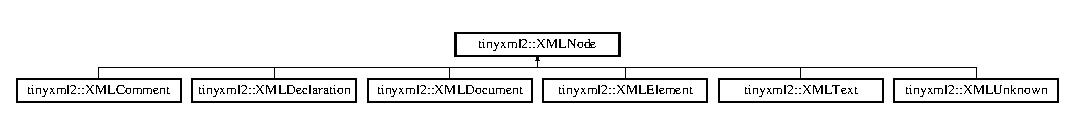
\includegraphics[height=1.145194cm]{classtinyxml2_1_1_x_m_l_node}
\end{center}
\end{figure}
\subsection*{Public Member Functions}
\begin{DoxyCompactItemize}
\item 
const \hyperlink{classtinyxml2_1_1_x_m_l_document}{X\-M\-L\-Document} $\ast$ \hyperlink{classtinyxml2_1_1_x_m_l_node_add244bca368083fa29698db8dcf147ca}{Get\-Document} () const 
\begin{DoxyCompactList}\small\item\em Get the \hyperlink{classtinyxml2_1_1_x_m_l_document}{X\-M\-L\-Document} that owns this \hyperlink{classtinyxml2_1_1_x_m_l_node}{X\-M\-L\-Node}. \end{DoxyCompactList}\item 
\hyperlink{classtinyxml2_1_1_x_m_l_document}{X\-M\-L\-Document} $\ast$ \hyperlink{classtinyxml2_1_1_x_m_l_node_af343d1ef0b45c0020e62d784d7e67a68}{Get\-Document} ()
\begin{DoxyCompactList}\small\item\em Get the \hyperlink{classtinyxml2_1_1_x_m_l_document}{X\-M\-L\-Document} that owns this \hyperlink{classtinyxml2_1_1_x_m_l_node}{X\-M\-L\-Node}. \end{DoxyCompactList}\item 
virtual \hyperlink{classtinyxml2_1_1_x_m_l_element}{X\-M\-L\-Element} $\ast$ \hyperlink{classtinyxml2_1_1_x_m_l_node_aab516e699567f75cc9ab2ef2eee501e8}{To\-Element} ()
\begin{DoxyCompactList}\small\item\em Safely cast to an Element, or null. \end{DoxyCompactList}\item 
virtual \hyperlink{classtinyxml2_1_1_x_m_l_text}{X\-M\-L\-Text} $\ast$ \hyperlink{classtinyxml2_1_1_x_m_l_node_a41c55dab9162d1eb62db2008430e376b}{To\-Text} ()
\begin{DoxyCompactList}\small\item\em Safely cast to Text, or null. \end{DoxyCompactList}\item 
virtual \hyperlink{classtinyxml2_1_1_x_m_l_comment}{X\-M\-L\-Comment} $\ast$ \hyperlink{classtinyxml2_1_1_x_m_l_node_aff47671055aa99840a1c1ebd661e63e3}{To\-Comment} ()
\begin{DoxyCompactList}\small\item\em Safely cast to a Comment, or null. \end{DoxyCompactList}\item 
virtual \hyperlink{classtinyxml2_1_1_x_m_l_document}{X\-M\-L\-Document} $\ast$ \hyperlink{classtinyxml2_1_1_x_m_l_node_a836e2966ed736fc3c94f70e12a2a3357}{To\-Document} ()
\begin{DoxyCompactList}\small\item\em Safely cast to a Document, or null. \end{DoxyCompactList}\item 
virtual \hyperlink{classtinyxml2_1_1_x_m_l_declaration}{X\-M\-L\-Declaration} $\ast$ \hyperlink{classtinyxml2_1_1_x_m_l_node_a174fd4c22c010b58138c1b84a0dfbd51}{To\-Declaration} ()
\begin{DoxyCompactList}\small\item\em Safely cast to a Declaration, or null. \end{DoxyCompactList}\item 
virtual \hyperlink{classtinyxml2_1_1_x_m_l_unknown}{X\-M\-L\-Unknown} $\ast$ \hyperlink{classtinyxml2_1_1_x_m_l_node_a8675a74aa0ada6eccab0c77ef3e5b9bd}{To\-Unknown} ()
\begin{DoxyCompactList}\small\item\em Safely cast to an Unknown, or null. \end{DoxyCompactList}\item 
virtual const \hyperlink{classtinyxml2_1_1_x_m_l_element}{X\-M\-L\-Element} $\ast$ \hyperlink{classtinyxml2_1_1_x_m_l_node_acbaec609797ddabb4f9dcf38ee91262e}{To\-Element} () const 
\item 
virtual const \hyperlink{classtinyxml2_1_1_x_m_l_text}{X\-M\-L\-Text} $\ast$ \hyperlink{classtinyxml2_1_1_x_m_l_node_a89009ffc1b9f5d692bf8d4c9f18c3bec}{To\-Text} () const 
\item 
virtual const \hyperlink{classtinyxml2_1_1_x_m_l_comment}{X\-M\-L\-Comment} $\ast$ \hyperlink{classtinyxml2_1_1_x_m_l_node_a157ce3a00ea5ee5a85b7103138e85e8a}{To\-Comment} () const 
\item 
virtual const \hyperlink{classtinyxml2_1_1_x_m_l_document}{X\-M\-L\-Document} $\ast$ \hyperlink{classtinyxml2_1_1_x_m_l_node_a3ff975733a17d6ced3539b45544c8bf6}{To\-Document} () const 
\item 
virtual const \hyperlink{classtinyxml2_1_1_x_m_l_declaration}{X\-M\-L\-Declaration} $\ast$ \hyperlink{classtinyxml2_1_1_x_m_l_node_aedae0bbb58d533a4b8a61042388b49e5}{To\-Declaration} () const 
\item 
virtual const \hyperlink{classtinyxml2_1_1_x_m_l_unknown}{X\-M\-L\-Unknown} $\ast$ \hyperlink{classtinyxml2_1_1_x_m_l_node_a71f5ae90296dbe67979f83fe97073efa}{To\-Unknown} () const 
\item 
const char $\ast$ \hyperlink{classtinyxml2_1_1_x_m_l_node_a7682be117e3b2b4ebfd517c1acaaadbf}{Value} () const 
\item 
void \hyperlink{classtinyxml2_1_1_x_m_l_node_a09dd68cf9eae137579f6e50f36487513}{Set\-Value} (const char $\ast$val, bool static\-Mem=false)
\item 
const \hyperlink{classtinyxml2_1_1_x_m_l_node}{X\-M\-L\-Node} $\ast$ \hyperlink{classtinyxml2_1_1_x_m_l_node_a4e39bdcf9bfafa55d04857ece6aaf64e}{Parent} () const 
\begin{DoxyCompactList}\small\item\em Get the parent of this node on the D\-O\-M. \end{DoxyCompactList}\item 
\hyperlink{classtinyxml2_1_1_x_m_l_node}{X\-M\-L\-Node} $\ast$ \hyperlink{classtinyxml2_1_1_x_m_l_node_a76029693a5a54fbb721a41d7a0ca8a97}{Parent} ()
\item 
bool \hyperlink{classtinyxml2_1_1_x_m_l_node_a96afe34a9ccd0ed4c0cff32beb42cc6c}{No\-Children} () const 
\begin{DoxyCompactList}\small\item\em Returns true if this node has no children. \end{DoxyCompactList}\item 
const \hyperlink{classtinyxml2_1_1_x_m_l_node}{X\-M\-L\-Node} $\ast$ \hyperlink{classtinyxml2_1_1_x_m_l_node_a60e923d13d7dc01f45ab90a2f948b02a}{First\-Child} () const 
\begin{DoxyCompactList}\small\item\em Get the first child node, or null if none exists. \end{DoxyCompactList}\item 
\hyperlink{classtinyxml2_1_1_x_m_l_node}{X\-M\-L\-Node} $\ast$ \hyperlink{classtinyxml2_1_1_x_m_l_node_a2d6c70c475146b48bc93a7fafdeff5e0}{First\-Child} ()
\item 
const \hyperlink{classtinyxml2_1_1_x_m_l_element}{X\-M\-L\-Element} $\ast$ \hyperlink{classtinyxml2_1_1_x_m_l_node_a20f48e99b03e9c17487944f229bee130}{First\-Child\-Element} (const char $\ast$value=0) const 
\item 
\hyperlink{classtinyxml2_1_1_x_m_l_element}{X\-M\-L\-Element} $\ast$ \hyperlink{classtinyxml2_1_1_x_m_l_node_a7614c3b4eea1ff11b2aa90b0f92f6dba}{First\-Child\-Element} (const char $\ast$value=0)
\item 
const \hyperlink{classtinyxml2_1_1_x_m_l_node}{X\-M\-L\-Node} $\ast$ \hyperlink{classtinyxml2_1_1_x_m_l_node_a6088246532b02895beb0e6fa561a7f3b}{Last\-Child} () const 
\begin{DoxyCompactList}\small\item\em Get the last child node, or null if none exists. \end{DoxyCompactList}\item 
\hyperlink{classtinyxml2_1_1_x_m_l_node}{X\-M\-L\-Node} $\ast$ \hyperlink{classtinyxml2_1_1_x_m_l_node_ad7552c8cb1dc0cb6f3bdc14a9d115dbf}{Last\-Child} ()
\item 
const \hyperlink{classtinyxml2_1_1_x_m_l_element}{X\-M\-L\-Element} $\ast$ \hyperlink{classtinyxml2_1_1_x_m_l_node_a1a46cc01ece2216acf1e6294d1aff79d}{Last\-Child\-Element} (const char $\ast$value=0) const 
\item 
\hyperlink{classtinyxml2_1_1_x_m_l_element}{X\-M\-L\-Element} $\ast$ \hyperlink{classtinyxml2_1_1_x_m_l_node_a125423acf3170b130634638c5afc0639}{Last\-Child\-Element} (const char $\ast$value=0)
\item 
const \hyperlink{classtinyxml2_1_1_x_m_l_node}{X\-M\-L\-Node} $\ast$ \hyperlink{classtinyxml2_1_1_x_m_l_node_a4cb1bf63e9de55129d21a7be60685fd4}{Previous\-Sibling} () const 
\begin{DoxyCompactList}\small\item\em Get the previous (left) sibling node of this node. \end{DoxyCompactList}\item 
\hyperlink{classtinyxml2_1_1_x_m_l_node}{X\-M\-L\-Node} $\ast$ \hyperlink{classtinyxml2_1_1_x_m_l_node_ae760e5e7e766df1d2cf3bb4a847876d6}{Previous\-Sibling} ()
\item 
const \hyperlink{classtinyxml2_1_1_x_m_l_element}{X\-M\-L\-Element} $\ast$ \hyperlink{classtinyxml2_1_1_x_m_l_node_a573b2559c41dce244d893d610fbe0bd9}{Previous\-Sibling\-Element} (const char $\ast$value=0) const 
\begin{DoxyCompactList}\small\item\em Get the previous (left) sibling element of this node, with an optionally supplied name. \end{DoxyCompactList}\item 
\hyperlink{classtinyxml2_1_1_x_m_l_element}{X\-M\-L\-Element} $\ast$ \hyperlink{classtinyxml2_1_1_x_m_l_node_ae9177fdc49cb89879f333581d5f734f1}{Previous\-Sibling\-Element} (const char $\ast$value=0)
\item 
const \hyperlink{classtinyxml2_1_1_x_m_l_node}{X\-M\-L\-Node} $\ast$ \hyperlink{classtinyxml2_1_1_x_m_l_node_abba1df37581d89dccc45acdc55750ba2}{Next\-Sibling} () const 
\begin{DoxyCompactList}\small\item\em Get the next (right) sibling node of this node. \end{DoxyCompactList}\item 
\hyperlink{classtinyxml2_1_1_x_m_l_node}{X\-M\-L\-Node} $\ast$ \hyperlink{classtinyxml2_1_1_x_m_l_node_aeb7d4dfd8fb924ef86e7cb72183acbac}{Next\-Sibling} ()
\item 
const \hyperlink{classtinyxml2_1_1_x_m_l_element}{X\-M\-L\-Element} $\ast$ \hyperlink{classtinyxml2_1_1_x_m_l_node_a490e166c3a1c6607960bfa9c112d3d30}{Next\-Sibling\-Element} (const char $\ast$value=0) const 
\begin{DoxyCompactList}\small\item\em Get the next (right) sibling element of this node, with an optionally supplied name. \end{DoxyCompactList}\item 
\hyperlink{classtinyxml2_1_1_x_m_l_element}{X\-M\-L\-Element} $\ast$ \hyperlink{classtinyxml2_1_1_x_m_l_node_acf735bf653016792522305d8ad4b3029}{Next\-Sibling\-Element} (const char $\ast$value=0)
\item 
\hyperlink{classtinyxml2_1_1_x_m_l_node}{X\-M\-L\-Node} $\ast$ \hyperlink{classtinyxml2_1_1_x_m_l_node_ae3b422e98914d6002ca99bb1d2837103}{Insert\-End\-Child} (\hyperlink{classtinyxml2_1_1_x_m_l_node}{X\-M\-L\-Node} $\ast$add\-This)
\item 
\hyperlink{classtinyxml2_1_1_x_m_l_node}{X\-M\-L\-Node} $\ast$ \hyperlink{classtinyxml2_1_1_x_m_l_node_a663e3a5a378169fd477378f4d17a7649}{Link\-End\-Child} (\hyperlink{classtinyxml2_1_1_x_m_l_node}{X\-M\-L\-Node} $\ast$add\-This)
\item 
\hyperlink{classtinyxml2_1_1_x_m_l_node}{X\-M\-L\-Node} $\ast$ \hyperlink{classtinyxml2_1_1_x_m_l_node_ac609a8f3ea949027f439280c640bbaf2}{Insert\-First\-Child} (\hyperlink{classtinyxml2_1_1_x_m_l_node}{X\-M\-L\-Node} $\ast$add\-This)
\item 
\hyperlink{classtinyxml2_1_1_x_m_l_node}{X\-M\-L\-Node} $\ast$ \hyperlink{classtinyxml2_1_1_x_m_l_node_a9275138a1b8dd5d8e2c26789bdc23ac8}{Insert\-After\-Child} (\hyperlink{classtinyxml2_1_1_x_m_l_node}{X\-M\-L\-Node} $\ast$after\-This, \hyperlink{classtinyxml2_1_1_x_m_l_node}{X\-M\-L\-Node} $\ast$add\-This)
\item 
void \hyperlink{classtinyxml2_1_1_x_m_l_node_a0360085cc54df5bff85d5c5da13afdce}{Delete\-Children} ()
\item 
void \hyperlink{classtinyxml2_1_1_x_m_l_node_a363b6edbd6ebd55f8387d2b89f2b0921}{Delete\-Child} (\hyperlink{classtinyxml2_1_1_x_m_l_node}{X\-M\-L\-Node} $\ast$node)
\item 
virtual \hyperlink{classtinyxml2_1_1_x_m_l_node}{X\-M\-L\-Node} $\ast$ \hyperlink{classtinyxml2_1_1_x_m_l_node_a8402cbd3129d20e9e6024bbcc0531283}{Shallow\-Clone} (\hyperlink{classtinyxml2_1_1_x_m_l_document}{X\-M\-L\-Document} $\ast$document) const =0
\item 
virtual bool \hyperlink{classtinyxml2_1_1_x_m_l_node_a7ce18b751c3ea09eac292dca264f9226}{Shallow\-Equal} (const \hyperlink{classtinyxml2_1_1_x_m_l_node}{X\-M\-L\-Node} $\ast$compare) const =0
\item 
virtual bool \hyperlink{classtinyxml2_1_1_x_m_l_node_a81e66df0a44c67a7af17f3b77a152785}{Accept} (\hyperlink{classtinyxml2_1_1_x_m_l_visitor}{X\-M\-L\-Visitor} $\ast$visitor) const =0
\item 
virtual char $\ast$ \hyperlink{classtinyxml2_1_1_x_m_l_node_a7610d0f603e8b603d2078521811a23c1}{Parse\-Deep} (char $\ast$, \hyperlink{classtinyxml2_1_1_str_pair}{Str\-Pair} $\ast$)
\end{DoxyCompactItemize}
\subsection*{Protected Member Functions}
\begin{DoxyCompactItemize}
\item 
\hyperlink{classtinyxml2_1_1_x_m_l_node_a29868df6ca383d574f584dfdd15105b6}{X\-M\-L\-Node} (\hyperlink{classtinyxml2_1_1_x_m_l_document}{X\-M\-L\-Document} $\ast$)
\item 
virtual \hyperlink{classtinyxml2_1_1_x_m_l_node_a8f41e898cdd4da4cdbb7f05b0c7d9f69}{$\sim$\-X\-M\-L\-Node} ()
\item 
\hyperlink{classtinyxml2_1_1_x_m_l_node_a78be01384518a969da905548f318d75b}{X\-M\-L\-Node} (const \hyperlink{classtinyxml2_1_1_x_m_l_node}{X\-M\-L\-Node} \&)
\item 
\hyperlink{classtinyxml2_1_1_x_m_l_node}{X\-M\-L\-Node} \& \hyperlink{classtinyxml2_1_1_x_m_l_node_ade79231d908e1f21862819e00e56ab6e}{operator=} (const \hyperlink{classtinyxml2_1_1_x_m_l_node}{X\-M\-L\-Node} \&)
\end{DoxyCompactItemize}
\subsection*{Protected Attributes}
\begin{DoxyCompactItemize}
\item 
\hyperlink{classtinyxml2_1_1_x_m_l_document}{X\-M\-L\-Document} $\ast$ \hyperlink{classtinyxml2_1_1_x_m_l_node_a8d2d2be0bb6797625551eb0e91f0ff62}{\-\_\-document}
\item 
\hyperlink{classtinyxml2_1_1_x_m_l_node}{X\-M\-L\-Node} $\ast$ \hyperlink{classtinyxml2_1_1_x_m_l_node_a176dd1c4965c21c366de192164aa2c13}{\-\_\-parent}
\item 
\hyperlink{classtinyxml2_1_1_str_pair}{Str\-Pair} \hyperlink{classtinyxml2_1_1_x_m_l_node_a3ea9884098b8379de2bb5ab3fc85c0fc}{\-\_\-value}
\item 
\hyperlink{classtinyxml2_1_1_x_m_l_node}{X\-M\-L\-Node} $\ast$ \hyperlink{classtinyxml2_1_1_x_m_l_node_aa20c91e4213dc930c5bdf420322ca342}{\-\_\-first\-Child}
\item 
\hyperlink{classtinyxml2_1_1_x_m_l_node}{X\-M\-L\-Node} $\ast$ \hyperlink{classtinyxml2_1_1_x_m_l_node_a099b6560ae44ab9edb8453aaf1a3747b}{\-\_\-last\-Child}
\item 
\hyperlink{classtinyxml2_1_1_x_m_l_node}{X\-M\-L\-Node} $\ast$ \hyperlink{classtinyxml2_1_1_x_m_l_node_a9739eb0fb9a1188266052055e7a6bf6b}{\-\_\-prev}
\item 
\hyperlink{classtinyxml2_1_1_x_m_l_node}{X\-M\-L\-Node} $\ast$ \hyperlink{classtinyxml2_1_1_x_m_l_node_a27e985496b37dd00eb5b9cf59b9e3fb1}{\-\_\-next}
\end{DoxyCompactItemize}
\subsection*{Friends}
\begin{DoxyCompactItemize}
\item 
class \hyperlink{classtinyxml2_1_1_x_m_l_node_a4eee3bda60c60a30e4e8cd4ea91c4c6e}{X\-M\-L\-Document}
\item 
class \hyperlink{classtinyxml2_1_1_x_m_l_node_ac2fba9b6e452829dd892f7392c24e0eb}{X\-M\-L\-Element}
\end{DoxyCompactItemize}


\subsection{Detailed Description}
\hyperlink{classtinyxml2_1_1_x_m_l_node}{X\-M\-L\-Node} is a base class for every object that is in the \hyperlink{namespace_x_m_l}{X\-M\-L} Document Object Model (D\-O\-M), except X\-M\-L\-Attributes. Nodes have siblings, a parent, and children which can be navigated. A node is always in a \hyperlink{classtinyxml2_1_1_x_m_l_document}{X\-M\-L\-Document}. The type of a \hyperlink{classtinyxml2_1_1_x_m_l_node}{X\-M\-L\-Node} can be queried, and it can be cast to its more defined type.

A \hyperlink{classtinyxml2_1_1_x_m_l_document}{X\-M\-L\-Document} allocates memory for all its Nodes. When the \hyperlink{classtinyxml2_1_1_x_m_l_document}{X\-M\-L\-Document} gets deleted, all its Nodes will also be deleted.

\begin{DoxyVerb}A Document can contain: Element (container or leaf)
                        Comment (leaf)
                        Unknown (leaf)
                        Declaration( leaf )

An Element can contain: Element (container or leaf)
                        Text    (leaf)
                        Attributes (not on tree)
                        Comment (leaf)
                        Unknown (leaf)\end{DoxyVerb}
 

Definition at line 573 of file tinyxml2.\-hpp.



\subsection{Constructor \& Destructor Documentation}
\hypertarget{classtinyxml2_1_1_x_m_l_node_a29868df6ca383d574f584dfdd15105b6}{\index{tinyxml2\-::\-X\-M\-L\-Node@{tinyxml2\-::\-X\-M\-L\-Node}!X\-M\-L\-Node@{X\-M\-L\-Node}}
\index{X\-M\-L\-Node@{X\-M\-L\-Node}!tinyxml2::XMLNode@{tinyxml2\-::\-X\-M\-L\-Node}}
\subsubsection[{X\-M\-L\-Node}]{\setlength{\rightskip}{0pt plus 5cm}tinyxml2\-::\-X\-M\-L\-Node\-::\-X\-M\-L\-Node (
\begin{DoxyParamCaption}
\item[{{\bf X\-M\-L\-Document} $\ast$}]{doc}
\end{DoxyParamCaption}
)\hspace{0.3cm}{\ttfamily [protected]}}}\label{classtinyxml2_1_1_x_m_l_node_a29868df6ca383d574f584dfdd15105b6}


Definition at line 580 of file tinyxml2.\-cpp.

\hypertarget{classtinyxml2_1_1_x_m_l_node_a8f41e898cdd4da4cdbb7f05b0c7d9f69}{\index{tinyxml2\-::\-X\-M\-L\-Node@{tinyxml2\-::\-X\-M\-L\-Node}!$\sim$\-X\-M\-L\-Node@{$\sim$\-X\-M\-L\-Node}}
\index{$\sim$\-X\-M\-L\-Node@{$\sim$\-X\-M\-L\-Node}!tinyxml2::XMLNode@{tinyxml2\-::\-X\-M\-L\-Node}}
\subsubsection[{$\sim$\-X\-M\-L\-Node}]{\setlength{\rightskip}{0pt plus 5cm}tinyxml2\-::\-X\-M\-L\-Node\-::$\sim$\-X\-M\-L\-Node (
\begin{DoxyParamCaption}
{}
\end{DoxyParamCaption}
)\hspace{0.3cm}{\ttfamily [protected]}, {\ttfamily [virtual]}}}\label{classtinyxml2_1_1_x_m_l_node_a8f41e898cdd4da4cdbb7f05b0c7d9f69}


Definition at line 590 of file tinyxml2.\-cpp.

\hypertarget{classtinyxml2_1_1_x_m_l_node_a78be01384518a969da905548f318d75b}{\index{tinyxml2\-::\-X\-M\-L\-Node@{tinyxml2\-::\-X\-M\-L\-Node}!X\-M\-L\-Node@{X\-M\-L\-Node}}
\index{X\-M\-L\-Node@{X\-M\-L\-Node}!tinyxml2::XMLNode@{tinyxml2\-::\-X\-M\-L\-Node}}
\subsubsection[{X\-M\-L\-Node}]{\setlength{\rightskip}{0pt plus 5cm}tinyxml2\-::\-X\-M\-L\-Node\-::\-X\-M\-L\-Node (
\begin{DoxyParamCaption}
\item[{const {\bf X\-M\-L\-Node} \&}]{}
\end{DoxyParamCaption}
)\hspace{0.3cm}{\ttfamily [protected]}}}\label{classtinyxml2_1_1_x_m_l_node_a78be01384518a969da905548f318d75b}


\subsection{Member Function Documentation}
\hypertarget{classtinyxml2_1_1_x_m_l_node_a81e66df0a44c67a7af17f3b77a152785}{\index{tinyxml2\-::\-X\-M\-L\-Node@{tinyxml2\-::\-X\-M\-L\-Node}!Accept@{Accept}}
\index{Accept@{Accept}!tinyxml2::XMLNode@{tinyxml2\-::\-X\-M\-L\-Node}}
\subsubsection[{Accept}]{\setlength{\rightskip}{0pt plus 5cm}virtual bool tinyxml2\-::\-X\-M\-L\-Node\-::\-Accept (
\begin{DoxyParamCaption}
\item[{{\bf X\-M\-L\-Visitor} $\ast$}]{visitor}
\end{DoxyParamCaption}
) const\hspace{0.3cm}{\ttfamily [pure virtual]}}}\label{classtinyxml2_1_1_x_m_l_node_a81e66df0a44c67a7af17f3b77a152785}
Accept a hierarchical visit of the nodes in the Tiny\-X\-M\-L-\/2 D\-O\-M. Every node in the \hyperlink{namespace_x_m_l}{X\-M\-L} tree will be conditionally visited and the host will be called back via the \hyperlink{classtinyxml2_1_1_x_m_l_visitor}{X\-M\-L\-Visitor} interface.

This is essentially a S\-A\-X interface for Tiny\-X\-M\-L-\/2. (Note however it doesn't re-\/parse the \hyperlink{namespace_x_m_l}{X\-M\-L} for the callbacks, so the performance of Tiny\-X\-M\-L-\/2 is unchanged by using this interface versus any other.)

The interface has been based on ideas from\-:


\begin{DoxyItemize}
\item \href{http://www.saxproject.org/}{\tt http\-://www.\-saxproject.\-org/}
\item \href{http://c2.com/cgi/wiki?HierarchicalVisitorPattern}{\tt http\-://c2.\-com/cgi/wiki?\-Hierarchical\-Visitor\-Pattern}
\end{DoxyItemize}

Which are both good references for \char`\"{}visiting\char`\"{}.

An example of using \hyperlink{classtinyxml2_1_1_x_m_l_node_a81e66df0a44c67a7af17f3b77a152785}{Accept()}\-: \begin{DoxyVerb}XMLPrinter printer;
tinyxmlDoc.Accept( &printer );
const char* xmlcstr = printer.CStr();
\end{DoxyVerb}
 

Implemented in \hyperlink{classtinyxml2_1_1_x_m_l_document_aa08503d24898bf9992ae5e5fb8b0cf87}{tinyxml2\-::\-X\-M\-L\-Document}, \hyperlink{classtinyxml2_1_1_x_m_l_element_a36d65438991a1e85096caf39ad13a099}{tinyxml2\-::\-X\-M\-L\-Element}, \hyperlink{classtinyxml2_1_1_x_m_l_unknown_a0d341ab804a1438a474810bb5bd29dd5}{tinyxml2\-::\-X\-M\-L\-Unknown}, \hyperlink{classtinyxml2_1_1_x_m_l_declaration_a953a7359cc312d15218eb5843a4ca108}{tinyxml2\-::\-X\-M\-L\-Declaration}, \hyperlink{classtinyxml2_1_1_x_m_l_comment_aa382b1be6a8b0650c16a2d88bb499335}{tinyxml2\-::\-X\-M\-L\-Comment}, and \hyperlink{classtinyxml2_1_1_x_m_l_text_ae659d4fc7351a7df11c111cbe1ade46f}{tinyxml2\-::\-X\-M\-L\-Text}.

\hypertarget{classtinyxml2_1_1_x_m_l_node_a363b6edbd6ebd55f8387d2b89f2b0921}{\index{tinyxml2\-::\-X\-M\-L\-Node@{tinyxml2\-::\-X\-M\-L\-Node}!Delete\-Child@{Delete\-Child}}
\index{Delete\-Child@{Delete\-Child}!tinyxml2::XMLNode@{tinyxml2\-::\-X\-M\-L\-Node}}
\subsubsection[{Delete\-Child}]{\setlength{\rightskip}{0pt plus 5cm}void tinyxml2\-::\-X\-M\-L\-Node\-::\-Delete\-Child (
\begin{DoxyParamCaption}
\item[{{\bf X\-M\-L\-Node} $\ast$}]{node}
\end{DoxyParamCaption}
)}}\label{classtinyxml2_1_1_x_m_l_node_a363b6edbd6ebd55f8387d2b89f2b0921}
Delete a child of this node. 

Definition at line 642 of file tinyxml2.\-cpp.

\hypertarget{classtinyxml2_1_1_x_m_l_node_a0360085cc54df5bff85d5c5da13afdce}{\index{tinyxml2\-::\-X\-M\-L\-Node@{tinyxml2\-::\-X\-M\-L\-Node}!Delete\-Children@{Delete\-Children}}
\index{Delete\-Children@{Delete\-Children}!tinyxml2::XMLNode@{tinyxml2\-::\-X\-M\-L\-Node}}
\subsubsection[{Delete\-Children}]{\setlength{\rightskip}{0pt plus 5cm}void tinyxml2\-::\-X\-M\-L\-Node\-::\-Delete\-Children (
\begin{DoxyParamCaption}
{}
\end{DoxyParamCaption}
)}}\label{classtinyxml2_1_1_x_m_l_node_a0360085cc54df5bff85d5c5da13afdce}
Delete all the children of this node. 

Definition at line 610 of file tinyxml2.\-cpp.

\hypertarget{classtinyxml2_1_1_x_m_l_node_a60e923d13d7dc01f45ab90a2f948b02a}{\index{tinyxml2\-::\-X\-M\-L\-Node@{tinyxml2\-::\-X\-M\-L\-Node}!First\-Child@{First\-Child}}
\index{First\-Child@{First\-Child}!tinyxml2::XMLNode@{tinyxml2\-::\-X\-M\-L\-Node}}
\subsubsection[{First\-Child}]{\setlength{\rightskip}{0pt plus 5cm}const {\bf X\-M\-L\-Node}$\ast$ tinyxml2\-::\-X\-M\-L\-Node\-::\-First\-Child (
\begin{DoxyParamCaption}
{}
\end{DoxyParamCaption}
) const\hspace{0.3cm}{\ttfamily [inline]}}}\label{classtinyxml2_1_1_x_m_l_node_a60e923d13d7dc01f45ab90a2f948b02a}


Get the first child node, or null if none exists. 



Definition at line 665 of file tinyxml2.\-hpp.

\hypertarget{classtinyxml2_1_1_x_m_l_node_a2d6c70c475146b48bc93a7fafdeff5e0}{\index{tinyxml2\-::\-X\-M\-L\-Node@{tinyxml2\-::\-X\-M\-L\-Node}!First\-Child@{First\-Child}}
\index{First\-Child@{First\-Child}!tinyxml2::XMLNode@{tinyxml2\-::\-X\-M\-L\-Node}}
\subsubsection[{First\-Child}]{\setlength{\rightskip}{0pt plus 5cm}{\bf X\-M\-L\-Node}$\ast$ tinyxml2\-::\-X\-M\-L\-Node\-::\-First\-Child (
\begin{DoxyParamCaption}
{}
\end{DoxyParamCaption}
)\hspace{0.3cm}{\ttfamily [inline]}}}\label{classtinyxml2_1_1_x_m_l_node_a2d6c70c475146b48bc93a7fafdeff5e0}


Definition at line 669 of file tinyxml2.\-hpp.

\hypertarget{classtinyxml2_1_1_x_m_l_node_a20f48e99b03e9c17487944f229bee130}{\index{tinyxml2\-::\-X\-M\-L\-Node@{tinyxml2\-::\-X\-M\-L\-Node}!First\-Child\-Element@{First\-Child\-Element}}
\index{First\-Child\-Element@{First\-Child\-Element}!tinyxml2::XMLNode@{tinyxml2\-::\-X\-M\-L\-Node}}
\subsubsection[{First\-Child\-Element}]{\setlength{\rightskip}{0pt plus 5cm}const {\bf X\-M\-L\-Element} $\ast$ tinyxml2\-::\-X\-M\-L\-Node\-::\-First\-Child\-Element (
\begin{DoxyParamCaption}
\item[{const char $\ast$}]{value = {\ttfamily 0}}
\end{DoxyParamCaption}
) const}}\label{classtinyxml2_1_1_x_m_l_node_a20f48e99b03e9c17487944f229bee130}
Get the first child element, or optionally the first child element with the specified name. 

Definition at line 721 of file tinyxml2.\-cpp.

\hypertarget{classtinyxml2_1_1_x_m_l_node_a7614c3b4eea1ff11b2aa90b0f92f6dba}{\index{tinyxml2\-::\-X\-M\-L\-Node@{tinyxml2\-::\-X\-M\-L\-Node}!First\-Child\-Element@{First\-Child\-Element}}
\index{First\-Child\-Element@{First\-Child\-Element}!tinyxml2::XMLNode@{tinyxml2\-::\-X\-M\-L\-Node}}
\subsubsection[{First\-Child\-Element}]{\setlength{\rightskip}{0pt plus 5cm}{\bf X\-M\-L\-Element}$\ast$ tinyxml2\-::\-X\-M\-L\-Node\-::\-First\-Child\-Element (
\begin{DoxyParamCaption}
\item[{const char $\ast$}]{value = {\ttfamily 0}}
\end{DoxyParamCaption}
)\hspace{0.3cm}{\ttfamily [inline]}}}\label{classtinyxml2_1_1_x_m_l_node_a7614c3b4eea1ff11b2aa90b0f92f6dba}


Definition at line 678 of file tinyxml2.\-hpp.

\hypertarget{classtinyxml2_1_1_x_m_l_node_add244bca368083fa29698db8dcf147ca}{\index{tinyxml2\-::\-X\-M\-L\-Node@{tinyxml2\-::\-X\-M\-L\-Node}!Get\-Document@{Get\-Document}}
\index{Get\-Document@{Get\-Document}!tinyxml2::XMLNode@{tinyxml2\-::\-X\-M\-L\-Node}}
\subsubsection[{Get\-Document}]{\setlength{\rightskip}{0pt plus 5cm}const {\bf X\-M\-L\-Document}$\ast$ tinyxml2\-::\-X\-M\-L\-Node\-::\-Get\-Document (
\begin{DoxyParamCaption}
{}
\end{DoxyParamCaption}
) const\hspace{0.3cm}{\ttfamily [inline]}}}\label{classtinyxml2_1_1_x_m_l_node_add244bca368083fa29698db8dcf147ca}


Get the \hyperlink{classtinyxml2_1_1_x_m_l_document}{X\-M\-L\-Document} that owns this \hyperlink{classtinyxml2_1_1_x_m_l_node}{X\-M\-L\-Node}. 



Definition at line 580 of file tinyxml2.\-hpp.

\hypertarget{classtinyxml2_1_1_x_m_l_node_af343d1ef0b45c0020e62d784d7e67a68}{\index{tinyxml2\-::\-X\-M\-L\-Node@{tinyxml2\-::\-X\-M\-L\-Node}!Get\-Document@{Get\-Document}}
\index{Get\-Document@{Get\-Document}!tinyxml2::XMLNode@{tinyxml2\-::\-X\-M\-L\-Node}}
\subsubsection[{Get\-Document}]{\setlength{\rightskip}{0pt plus 5cm}{\bf X\-M\-L\-Document}$\ast$ tinyxml2\-::\-X\-M\-L\-Node\-::\-Get\-Document (
\begin{DoxyParamCaption}
{}
\end{DoxyParamCaption}
)\hspace{0.3cm}{\ttfamily [inline]}}}\label{classtinyxml2_1_1_x_m_l_node_af343d1ef0b45c0020e62d784d7e67a68}


Get the \hyperlink{classtinyxml2_1_1_x_m_l_document}{X\-M\-L\-Document} that owns this \hyperlink{classtinyxml2_1_1_x_m_l_node}{X\-M\-L\-Node}. 



Definition at line 584 of file tinyxml2.\-hpp.

\hypertarget{classtinyxml2_1_1_x_m_l_node_a9275138a1b8dd5d8e2c26789bdc23ac8}{\index{tinyxml2\-::\-X\-M\-L\-Node@{tinyxml2\-::\-X\-M\-L\-Node}!Insert\-After\-Child@{Insert\-After\-Child}}
\index{Insert\-After\-Child@{Insert\-After\-Child}!tinyxml2::XMLNode@{tinyxml2\-::\-X\-M\-L\-Node}}
\subsubsection[{Insert\-After\-Child}]{\setlength{\rightskip}{0pt plus 5cm}{\bf X\-M\-L\-Node} $\ast$ tinyxml2\-::\-X\-M\-L\-Node\-::\-Insert\-After\-Child (
\begin{DoxyParamCaption}
\item[{{\bf X\-M\-L\-Node} $\ast$}]{after\-This, }
\item[{{\bf X\-M\-L\-Node} $\ast$}]{add\-This}
\end{DoxyParamCaption}
)}}\label{classtinyxml2_1_1_x_m_l_node_a9275138a1b8dd5d8e2c26789bdc23ac8}
Add a node after the specified child node. 

Definition at line 698 of file tinyxml2.\-cpp.

\hypertarget{classtinyxml2_1_1_x_m_l_node_ae3b422e98914d6002ca99bb1d2837103}{\index{tinyxml2\-::\-X\-M\-L\-Node@{tinyxml2\-::\-X\-M\-L\-Node}!Insert\-End\-Child@{Insert\-End\-Child}}
\index{Insert\-End\-Child@{Insert\-End\-Child}!tinyxml2::XMLNode@{tinyxml2\-::\-X\-M\-L\-Node}}
\subsubsection[{Insert\-End\-Child}]{\setlength{\rightskip}{0pt plus 5cm}{\bf X\-M\-L\-Node} $\ast$ tinyxml2\-::\-X\-M\-L\-Node\-::\-Insert\-End\-Child (
\begin{DoxyParamCaption}
\item[{{\bf X\-M\-L\-Node} $\ast$}]{add\-This}
\end{DoxyParamCaption}
)}}\label{classtinyxml2_1_1_x_m_l_node_ae3b422e98914d6002ca99bb1d2837103}
Add a child node as the last (right) child. 

Definition at line 649 of file tinyxml2.\-cpp.

\hypertarget{classtinyxml2_1_1_x_m_l_node_ac609a8f3ea949027f439280c640bbaf2}{\index{tinyxml2\-::\-X\-M\-L\-Node@{tinyxml2\-::\-X\-M\-L\-Node}!Insert\-First\-Child@{Insert\-First\-Child}}
\index{Insert\-First\-Child@{Insert\-First\-Child}!tinyxml2::XMLNode@{tinyxml2\-::\-X\-M\-L\-Node}}
\subsubsection[{Insert\-First\-Child}]{\setlength{\rightskip}{0pt plus 5cm}{\bf X\-M\-L\-Node} $\ast$ tinyxml2\-::\-X\-M\-L\-Node\-::\-Insert\-First\-Child (
\begin{DoxyParamCaption}
\item[{{\bf X\-M\-L\-Node} $\ast$}]{add\-This}
\end{DoxyParamCaption}
)}}\label{classtinyxml2_1_1_x_m_l_node_ac609a8f3ea949027f439280c640bbaf2}
Add a child node as the first (left) child. 

Definition at line 673 of file tinyxml2.\-cpp.

\hypertarget{classtinyxml2_1_1_x_m_l_node_a6088246532b02895beb0e6fa561a7f3b}{\index{tinyxml2\-::\-X\-M\-L\-Node@{tinyxml2\-::\-X\-M\-L\-Node}!Last\-Child@{Last\-Child}}
\index{Last\-Child@{Last\-Child}!tinyxml2::XMLNode@{tinyxml2\-::\-X\-M\-L\-Node}}
\subsubsection[{Last\-Child}]{\setlength{\rightskip}{0pt plus 5cm}const {\bf X\-M\-L\-Node}$\ast$ tinyxml2\-::\-X\-M\-L\-Node\-::\-Last\-Child (
\begin{DoxyParamCaption}
{}
\end{DoxyParamCaption}
) const\hspace{0.3cm}{\ttfamily [inline]}}}\label{classtinyxml2_1_1_x_m_l_node_a6088246532b02895beb0e6fa561a7f3b}


Get the last child node, or null if none exists. 



Definition at line 683 of file tinyxml2.\-hpp.

\hypertarget{classtinyxml2_1_1_x_m_l_node_ad7552c8cb1dc0cb6f3bdc14a9d115dbf}{\index{tinyxml2\-::\-X\-M\-L\-Node@{tinyxml2\-::\-X\-M\-L\-Node}!Last\-Child@{Last\-Child}}
\index{Last\-Child@{Last\-Child}!tinyxml2::XMLNode@{tinyxml2\-::\-X\-M\-L\-Node}}
\subsubsection[{Last\-Child}]{\setlength{\rightskip}{0pt plus 5cm}{\bf X\-M\-L\-Node}$\ast$ tinyxml2\-::\-X\-M\-L\-Node\-::\-Last\-Child (
\begin{DoxyParamCaption}
{}
\end{DoxyParamCaption}
)\hspace{0.3cm}{\ttfamily [inline]}}}\label{classtinyxml2_1_1_x_m_l_node_ad7552c8cb1dc0cb6f3bdc14a9d115dbf}


Definition at line 687 of file tinyxml2.\-hpp.

\hypertarget{classtinyxml2_1_1_x_m_l_node_a1a46cc01ece2216acf1e6294d1aff79d}{\index{tinyxml2\-::\-X\-M\-L\-Node@{tinyxml2\-::\-X\-M\-L\-Node}!Last\-Child\-Element@{Last\-Child\-Element}}
\index{Last\-Child\-Element@{Last\-Child\-Element}!tinyxml2::XMLNode@{tinyxml2\-::\-X\-M\-L\-Node}}
\subsubsection[{Last\-Child\-Element}]{\setlength{\rightskip}{0pt plus 5cm}const {\bf X\-M\-L\-Element} $\ast$ tinyxml2\-::\-X\-M\-L\-Node\-::\-Last\-Child\-Element (
\begin{DoxyParamCaption}
\item[{const char $\ast$}]{value = {\ttfamily 0}}
\end{DoxyParamCaption}
) const}}\label{classtinyxml2_1_1_x_m_l_node_a1a46cc01ece2216acf1e6294d1aff79d}
Get the last child element or optionally the last child element with the specified name. 

Definition at line 735 of file tinyxml2.\-cpp.

\hypertarget{classtinyxml2_1_1_x_m_l_node_a125423acf3170b130634638c5afc0639}{\index{tinyxml2\-::\-X\-M\-L\-Node@{tinyxml2\-::\-X\-M\-L\-Node}!Last\-Child\-Element@{Last\-Child\-Element}}
\index{Last\-Child\-Element@{Last\-Child\-Element}!tinyxml2::XMLNode@{tinyxml2\-::\-X\-M\-L\-Node}}
\subsubsection[{Last\-Child\-Element}]{\setlength{\rightskip}{0pt plus 5cm}{\bf X\-M\-L\-Element}$\ast$ tinyxml2\-::\-X\-M\-L\-Node\-::\-Last\-Child\-Element (
\begin{DoxyParamCaption}
\item[{const char $\ast$}]{value = {\ttfamily 0}}
\end{DoxyParamCaption}
)\hspace{0.3cm}{\ttfamily [inline]}}}\label{classtinyxml2_1_1_x_m_l_node_a125423acf3170b130634638c5afc0639}


Definition at line 696 of file tinyxml2.\-hpp.

\hypertarget{classtinyxml2_1_1_x_m_l_node_a663e3a5a378169fd477378f4d17a7649}{\index{tinyxml2\-::\-X\-M\-L\-Node@{tinyxml2\-::\-X\-M\-L\-Node}!Link\-End\-Child@{Link\-End\-Child}}
\index{Link\-End\-Child@{Link\-End\-Child}!tinyxml2::XMLNode@{tinyxml2\-::\-X\-M\-L\-Node}}
\subsubsection[{Link\-End\-Child}]{\setlength{\rightskip}{0pt plus 5cm}{\bf X\-M\-L\-Node}$\ast$ tinyxml2\-::\-X\-M\-L\-Node\-::\-Link\-End\-Child (
\begin{DoxyParamCaption}
\item[{{\bf X\-M\-L\-Node} $\ast$}]{add\-This}
\end{DoxyParamCaption}
)\hspace{0.3cm}{\ttfamily [inline]}}}\label{classtinyxml2_1_1_x_m_l_node_a663e3a5a378169fd477378f4d17a7649}


Definition at line 737 of file tinyxml2.\-hpp.

\hypertarget{classtinyxml2_1_1_x_m_l_node_abba1df37581d89dccc45acdc55750ba2}{\index{tinyxml2\-::\-X\-M\-L\-Node@{tinyxml2\-::\-X\-M\-L\-Node}!Next\-Sibling@{Next\-Sibling}}
\index{Next\-Sibling@{Next\-Sibling}!tinyxml2::XMLNode@{tinyxml2\-::\-X\-M\-L\-Node}}
\subsubsection[{Next\-Sibling}]{\setlength{\rightskip}{0pt plus 5cm}const {\bf X\-M\-L\-Node}$\ast$ tinyxml2\-::\-X\-M\-L\-Node\-::\-Next\-Sibling (
\begin{DoxyParamCaption}
{}
\end{DoxyParamCaption}
) const\hspace{0.3cm}{\ttfamily [inline]}}}\label{classtinyxml2_1_1_x_m_l_node_abba1df37581d89dccc45acdc55750ba2}


Get the next (right) sibling node of this node. 



Definition at line 717 of file tinyxml2.\-hpp.

\hypertarget{classtinyxml2_1_1_x_m_l_node_aeb7d4dfd8fb924ef86e7cb72183acbac}{\index{tinyxml2\-::\-X\-M\-L\-Node@{tinyxml2\-::\-X\-M\-L\-Node}!Next\-Sibling@{Next\-Sibling}}
\index{Next\-Sibling@{Next\-Sibling}!tinyxml2::XMLNode@{tinyxml2\-::\-X\-M\-L\-Node}}
\subsubsection[{Next\-Sibling}]{\setlength{\rightskip}{0pt plus 5cm}{\bf X\-M\-L\-Node}$\ast$ tinyxml2\-::\-X\-M\-L\-Node\-::\-Next\-Sibling (
\begin{DoxyParamCaption}
{}
\end{DoxyParamCaption}
)\hspace{0.3cm}{\ttfamily [inline]}}}\label{classtinyxml2_1_1_x_m_l_node_aeb7d4dfd8fb924ef86e7cb72183acbac}


Definition at line 721 of file tinyxml2.\-hpp.

\hypertarget{classtinyxml2_1_1_x_m_l_node_a490e166c3a1c6607960bfa9c112d3d30}{\index{tinyxml2\-::\-X\-M\-L\-Node@{tinyxml2\-::\-X\-M\-L\-Node}!Next\-Sibling\-Element@{Next\-Sibling\-Element}}
\index{Next\-Sibling\-Element@{Next\-Sibling\-Element}!tinyxml2::XMLNode@{tinyxml2\-::\-X\-M\-L\-Node}}
\subsubsection[{Next\-Sibling\-Element}]{\setlength{\rightskip}{0pt plus 5cm}const {\bf X\-M\-L\-Element} $\ast$ tinyxml2\-::\-X\-M\-L\-Node\-::\-Next\-Sibling\-Element (
\begin{DoxyParamCaption}
\item[{const char $\ast$}]{value = {\ttfamily 0}}
\end{DoxyParamCaption}
) const}}\label{classtinyxml2_1_1_x_m_l_node_a490e166c3a1c6607960bfa9c112d3d30}


Get the next (right) sibling element of this node, with an optionally supplied name. 



Definition at line 749 of file tinyxml2.\-cpp.

\hypertarget{classtinyxml2_1_1_x_m_l_node_acf735bf653016792522305d8ad4b3029}{\index{tinyxml2\-::\-X\-M\-L\-Node@{tinyxml2\-::\-X\-M\-L\-Node}!Next\-Sibling\-Element@{Next\-Sibling\-Element}}
\index{Next\-Sibling\-Element@{Next\-Sibling\-Element}!tinyxml2::XMLNode@{tinyxml2\-::\-X\-M\-L\-Node}}
\subsubsection[{Next\-Sibling\-Element}]{\setlength{\rightskip}{0pt plus 5cm}{\bf X\-M\-L\-Element}$\ast$ tinyxml2\-::\-X\-M\-L\-Node\-::\-Next\-Sibling\-Element (
\begin{DoxyParamCaption}
\item[{const char $\ast$}]{value = {\ttfamily 0}}
\end{DoxyParamCaption}
)\hspace{0.3cm}{\ttfamily [inline]}}}\label{classtinyxml2_1_1_x_m_l_node_acf735bf653016792522305d8ad4b3029}


Definition at line 728 of file tinyxml2.\-hpp.

\hypertarget{classtinyxml2_1_1_x_m_l_node_a96afe34a9ccd0ed4c0cff32beb42cc6c}{\index{tinyxml2\-::\-X\-M\-L\-Node@{tinyxml2\-::\-X\-M\-L\-Node}!No\-Children@{No\-Children}}
\index{No\-Children@{No\-Children}!tinyxml2::XMLNode@{tinyxml2\-::\-X\-M\-L\-Node}}
\subsubsection[{No\-Children}]{\setlength{\rightskip}{0pt plus 5cm}bool tinyxml2\-::\-X\-M\-L\-Node\-::\-No\-Children (
\begin{DoxyParamCaption}
{}
\end{DoxyParamCaption}
) const\hspace{0.3cm}{\ttfamily [inline]}}}\label{classtinyxml2_1_1_x_m_l_node_a96afe34a9ccd0ed4c0cff32beb42cc6c}


Returns true if this node has no children. 



Definition at line 660 of file tinyxml2.\-hpp.

\hypertarget{classtinyxml2_1_1_x_m_l_node_ade79231d908e1f21862819e00e56ab6e}{\index{tinyxml2\-::\-X\-M\-L\-Node@{tinyxml2\-::\-X\-M\-L\-Node}!operator=@{operator=}}
\index{operator=@{operator=}!tinyxml2::XMLNode@{tinyxml2\-::\-X\-M\-L\-Node}}
\subsubsection[{operator=}]{\setlength{\rightskip}{0pt plus 5cm}{\bf X\-M\-L\-Node}\& tinyxml2\-::\-X\-M\-L\-Node\-::operator= (
\begin{DoxyParamCaption}
\item[{const {\bf X\-M\-L\-Node} \&}]{}
\end{DoxyParamCaption}
)\hspace{0.3cm}{\ttfamily [protected]}}}\label{classtinyxml2_1_1_x_m_l_node_ade79231d908e1f21862819e00e56ab6e}
\hypertarget{classtinyxml2_1_1_x_m_l_node_a4e39bdcf9bfafa55d04857ece6aaf64e}{\index{tinyxml2\-::\-X\-M\-L\-Node@{tinyxml2\-::\-X\-M\-L\-Node}!Parent@{Parent}}
\index{Parent@{Parent}!tinyxml2::XMLNode@{tinyxml2\-::\-X\-M\-L\-Node}}
\subsubsection[{Parent}]{\setlength{\rightskip}{0pt plus 5cm}const {\bf X\-M\-L\-Node}$\ast$ tinyxml2\-::\-X\-M\-L\-Node\-::\-Parent (
\begin{DoxyParamCaption}
{}
\end{DoxyParamCaption}
) const\hspace{0.3cm}{\ttfamily [inline]}}}\label{classtinyxml2_1_1_x_m_l_node_a4e39bdcf9bfafa55d04857ece6aaf64e}


Get the parent of this node on the D\-O\-M. 



Definition at line 651 of file tinyxml2.\-hpp.

\hypertarget{classtinyxml2_1_1_x_m_l_node_a76029693a5a54fbb721a41d7a0ca8a97}{\index{tinyxml2\-::\-X\-M\-L\-Node@{tinyxml2\-::\-X\-M\-L\-Node}!Parent@{Parent}}
\index{Parent@{Parent}!tinyxml2::XMLNode@{tinyxml2\-::\-X\-M\-L\-Node}}
\subsubsection[{Parent}]{\setlength{\rightskip}{0pt plus 5cm}{\bf X\-M\-L\-Node}$\ast$ tinyxml2\-::\-X\-M\-L\-Node\-::\-Parent (
\begin{DoxyParamCaption}
{}
\end{DoxyParamCaption}
)\hspace{0.3cm}{\ttfamily [inline]}}}\label{classtinyxml2_1_1_x_m_l_node_a76029693a5a54fbb721a41d7a0ca8a97}


Definition at line 655 of file tinyxml2.\-hpp.

\hypertarget{classtinyxml2_1_1_x_m_l_node_a7610d0f603e8b603d2078521811a23c1}{\index{tinyxml2\-::\-X\-M\-L\-Node@{tinyxml2\-::\-X\-M\-L\-Node}!Parse\-Deep@{Parse\-Deep}}
\index{Parse\-Deep@{Parse\-Deep}!tinyxml2::XMLNode@{tinyxml2\-::\-X\-M\-L\-Node}}
\subsubsection[{Parse\-Deep}]{\setlength{\rightskip}{0pt plus 5cm}char $\ast$ tinyxml2\-::\-X\-M\-L\-Node\-::\-Parse\-Deep (
\begin{DoxyParamCaption}
\item[{char $\ast$}]{p, }
\item[{{\bf Str\-Pair} $\ast$}]{parent\-End}
\end{DoxyParamCaption}
)\hspace{0.3cm}{\ttfamily [virtual]}}}\label{classtinyxml2_1_1_x_m_l_node_a7610d0f603e8b603d2078521811a23c1}


Reimplemented in \hyperlink{classtinyxml2_1_1_x_m_l_element_aaafdd2a5618abe80a2c1839ad3ccd492}{tinyxml2\-::\-X\-M\-L\-Element}, \hyperlink{classtinyxml2_1_1_x_m_l_unknown_a0e4f3509dee42a4d45a7f0002be568cc}{tinyxml2\-::\-X\-M\-L\-Unknown}, \hyperlink{classtinyxml2_1_1_x_m_l_declaration_a19e33e0a9f9500f449261558c36f9a44}{tinyxml2\-::\-X\-M\-L\-Declaration}, \hyperlink{classtinyxml2_1_1_x_m_l_comment_aa6ab35c3bb1c1840371dc32a2040c57f}{tinyxml2\-::\-X\-M\-L\-Comment}, and \hyperlink{classtinyxml2_1_1_x_m_l_text_ac18d9eec9f12b827b0d02b0847bf279e}{tinyxml2\-::\-X\-M\-L\-Text}.



Definition at line 773 of file tinyxml2.\-cpp.

\hypertarget{classtinyxml2_1_1_x_m_l_node_a4cb1bf63e9de55129d21a7be60685fd4}{\index{tinyxml2\-::\-X\-M\-L\-Node@{tinyxml2\-::\-X\-M\-L\-Node}!Previous\-Sibling@{Previous\-Sibling}}
\index{Previous\-Sibling@{Previous\-Sibling}!tinyxml2::XMLNode@{tinyxml2\-::\-X\-M\-L\-Node}}
\subsubsection[{Previous\-Sibling}]{\setlength{\rightskip}{0pt plus 5cm}const {\bf X\-M\-L\-Node}$\ast$ tinyxml2\-::\-X\-M\-L\-Node\-::\-Previous\-Sibling (
\begin{DoxyParamCaption}
{}
\end{DoxyParamCaption}
) const\hspace{0.3cm}{\ttfamily [inline]}}}\label{classtinyxml2_1_1_x_m_l_node_a4cb1bf63e9de55129d21a7be60685fd4}


Get the previous (left) sibling node of this node. 



Definition at line 701 of file tinyxml2.\-hpp.

\hypertarget{classtinyxml2_1_1_x_m_l_node_ae760e5e7e766df1d2cf3bb4a847876d6}{\index{tinyxml2\-::\-X\-M\-L\-Node@{tinyxml2\-::\-X\-M\-L\-Node}!Previous\-Sibling@{Previous\-Sibling}}
\index{Previous\-Sibling@{Previous\-Sibling}!tinyxml2::XMLNode@{tinyxml2\-::\-X\-M\-L\-Node}}
\subsubsection[{Previous\-Sibling}]{\setlength{\rightskip}{0pt plus 5cm}{\bf X\-M\-L\-Node}$\ast$ tinyxml2\-::\-X\-M\-L\-Node\-::\-Previous\-Sibling (
\begin{DoxyParamCaption}
{}
\end{DoxyParamCaption}
)\hspace{0.3cm}{\ttfamily [inline]}}}\label{classtinyxml2_1_1_x_m_l_node_ae760e5e7e766df1d2cf3bb4a847876d6}


Definition at line 705 of file tinyxml2.\-hpp.

\hypertarget{classtinyxml2_1_1_x_m_l_node_a573b2559c41dce244d893d610fbe0bd9}{\index{tinyxml2\-::\-X\-M\-L\-Node@{tinyxml2\-::\-X\-M\-L\-Node}!Previous\-Sibling\-Element@{Previous\-Sibling\-Element}}
\index{Previous\-Sibling\-Element@{Previous\-Sibling\-Element}!tinyxml2::XMLNode@{tinyxml2\-::\-X\-M\-L\-Node}}
\subsubsection[{Previous\-Sibling\-Element}]{\setlength{\rightskip}{0pt plus 5cm}const {\bf X\-M\-L\-Element} $\ast$ tinyxml2\-::\-X\-M\-L\-Node\-::\-Previous\-Sibling\-Element (
\begin{DoxyParamCaption}
\item[{const char $\ast$}]{value = {\ttfamily 0}}
\end{DoxyParamCaption}
) const}}\label{classtinyxml2_1_1_x_m_l_node_a573b2559c41dce244d893d610fbe0bd9}


Get the previous (left) sibling element of this node, with an optionally supplied name. 



Definition at line 761 of file tinyxml2.\-cpp.

\hypertarget{classtinyxml2_1_1_x_m_l_node_ae9177fdc49cb89879f333581d5f734f1}{\index{tinyxml2\-::\-X\-M\-L\-Node@{tinyxml2\-::\-X\-M\-L\-Node}!Previous\-Sibling\-Element@{Previous\-Sibling\-Element}}
\index{Previous\-Sibling\-Element@{Previous\-Sibling\-Element}!tinyxml2::XMLNode@{tinyxml2\-::\-X\-M\-L\-Node}}
\subsubsection[{Previous\-Sibling\-Element}]{\setlength{\rightskip}{0pt plus 5cm}{\bf X\-M\-L\-Element}$\ast$ tinyxml2\-::\-X\-M\-L\-Node\-::\-Previous\-Sibling\-Element (
\begin{DoxyParamCaption}
\item[{const char $\ast$}]{value = {\ttfamily 0}}
\end{DoxyParamCaption}
)\hspace{0.3cm}{\ttfamily [inline]}}}\label{classtinyxml2_1_1_x_m_l_node_ae9177fdc49cb89879f333581d5f734f1}


Definition at line 712 of file tinyxml2.\-hpp.

\hypertarget{classtinyxml2_1_1_x_m_l_node_a09dd68cf9eae137579f6e50f36487513}{\index{tinyxml2\-::\-X\-M\-L\-Node@{tinyxml2\-::\-X\-M\-L\-Node}!Set\-Value@{Set\-Value}}
\index{Set\-Value@{Set\-Value}!tinyxml2::XMLNode@{tinyxml2\-::\-X\-M\-L\-Node}}
\subsubsection[{Set\-Value}]{\setlength{\rightskip}{0pt plus 5cm}void tinyxml2\-::\-X\-M\-L\-Node\-::\-Set\-Value (
\begin{DoxyParamCaption}
\item[{const char $\ast$}]{val, }
\item[{bool}]{static\-Mem = {\ttfamily false}}
\end{DoxyParamCaption}
)}}\label{classtinyxml2_1_1_x_m_l_node_a09dd68cf9eae137579f6e50f36487513}
Set the Value of an \hyperlink{namespace_x_m_l}{X\-M\-L} node. \begin{DoxySeeAlso}{See Also}
\hyperlink{classtinyxml2_1_1_x_m_l_node_a7682be117e3b2b4ebfd517c1acaaadbf}{Value()} 
\end{DoxySeeAlso}


Definition at line 599 of file tinyxml2.\-cpp.

\hypertarget{classtinyxml2_1_1_x_m_l_node_a8402cbd3129d20e9e6024bbcc0531283}{\index{tinyxml2\-::\-X\-M\-L\-Node@{tinyxml2\-::\-X\-M\-L\-Node}!Shallow\-Clone@{Shallow\-Clone}}
\index{Shallow\-Clone@{Shallow\-Clone}!tinyxml2::XMLNode@{tinyxml2\-::\-X\-M\-L\-Node}}
\subsubsection[{Shallow\-Clone}]{\setlength{\rightskip}{0pt plus 5cm}virtual {\bf X\-M\-L\-Node}$\ast$ tinyxml2\-::\-X\-M\-L\-Node\-::\-Shallow\-Clone (
\begin{DoxyParamCaption}
\item[{{\bf X\-M\-L\-Document} $\ast$}]{document}
\end{DoxyParamCaption}
) const\hspace{0.3cm}{\ttfamily [pure virtual]}}}\label{classtinyxml2_1_1_x_m_l_node_a8402cbd3129d20e9e6024bbcc0531283}
Make a copy of this node, but not its children. You may pass in a Document pointer that will be the owner of the new Node. If the 'document' is null, then the node returned will be allocated from the current Document. (this-\/$>$\hyperlink{classtinyxml2_1_1_x_m_l_node_af343d1ef0b45c0020e62d784d7e67a68}{Get\-Document()})

Note\-: if called on a \hyperlink{classtinyxml2_1_1_x_m_l_document}{X\-M\-L\-Document}, this will return null. 

Implemented in \hyperlink{classtinyxml2_1_1_x_m_l_document_a57c8511ed9f83aa3e20909a3db3f83d0}{tinyxml2\-::\-X\-M\-L\-Document}, \hyperlink{classtinyxml2_1_1_x_m_l_element_a85d85e32c18863fff1eeed53ae1ce23d}{tinyxml2\-::\-X\-M\-L\-Element}, \hyperlink{classtinyxml2_1_1_x_m_l_unknown_aa09fc7cb0cd64d6bb9c5ae00ffc549ec}{tinyxml2\-::\-X\-M\-L\-Unknown}, \hyperlink{classtinyxml2_1_1_x_m_l_declaration_a39458732ee6796cfc85dd35d3c488e0b}{tinyxml2\-::\-X\-M\-L\-Declaration}, \hyperlink{classtinyxml2_1_1_x_m_l_comment_a90bb60193a691b484f5e1b487857016d}{tinyxml2\-::\-X\-M\-L\-Comment}, and \hyperlink{classtinyxml2_1_1_x_m_l_text_af5115f8cc83de2947ed6a9d13e2f88c8}{tinyxml2\-::\-X\-M\-L\-Text}.

\hypertarget{classtinyxml2_1_1_x_m_l_node_a7ce18b751c3ea09eac292dca264f9226}{\index{tinyxml2\-::\-X\-M\-L\-Node@{tinyxml2\-::\-X\-M\-L\-Node}!Shallow\-Equal@{Shallow\-Equal}}
\index{Shallow\-Equal@{Shallow\-Equal}!tinyxml2::XMLNode@{tinyxml2\-::\-X\-M\-L\-Node}}
\subsubsection[{Shallow\-Equal}]{\setlength{\rightskip}{0pt plus 5cm}virtual bool tinyxml2\-::\-X\-M\-L\-Node\-::\-Shallow\-Equal (
\begin{DoxyParamCaption}
\item[{const {\bf X\-M\-L\-Node} $\ast$}]{compare}
\end{DoxyParamCaption}
) const\hspace{0.3cm}{\ttfamily [pure virtual]}}}\label{classtinyxml2_1_1_x_m_l_node_a7ce18b751c3ea09eac292dca264f9226}
Test if 2 nodes are the same, but don't test children. The 2 nodes do not need to be in the same Document.

Note\-: if called on a \hyperlink{classtinyxml2_1_1_x_m_l_document}{X\-M\-L\-Document}, this will return false. 

Implemented in \hyperlink{classtinyxml2_1_1_x_m_l_document_a12eac66c6e45d074d5cc47319868cd66}{tinyxml2\-::\-X\-M\-L\-Document}, \hyperlink{classtinyxml2_1_1_x_m_l_element_a25d51a2aad92625c78441457d58c85bc}{tinyxml2\-::\-X\-M\-L\-Element}, \hyperlink{classtinyxml2_1_1_x_m_l_unknown_a0169df157bf69a092b404ca49621ff1a}{tinyxml2\-::\-X\-M\-L\-Unknown}, \hyperlink{classtinyxml2_1_1_x_m_l_declaration_ace0d2d9bc1b63278bd5e984ebe0c7bd0}{tinyxml2\-::\-X\-M\-L\-Declaration}, \hyperlink{classtinyxml2_1_1_x_m_l_comment_a2d9f26757b0018fce933e74420cda22a}{tinyxml2\-::\-X\-M\-L\-Comment}, and \hyperlink{classtinyxml2_1_1_x_m_l_text_a1588aa5d23cb21eb31f36df0aaaa8d66}{tinyxml2\-::\-X\-M\-L\-Text}.

\hypertarget{classtinyxml2_1_1_x_m_l_node_aff47671055aa99840a1c1ebd661e63e3}{\index{tinyxml2\-::\-X\-M\-L\-Node@{tinyxml2\-::\-X\-M\-L\-Node}!To\-Comment@{To\-Comment}}
\index{To\-Comment@{To\-Comment}!tinyxml2::XMLNode@{tinyxml2\-::\-X\-M\-L\-Node}}
\subsubsection[{To\-Comment}]{\setlength{\rightskip}{0pt plus 5cm}virtual {\bf X\-M\-L\-Comment}$\ast$ tinyxml2\-::\-X\-M\-L\-Node\-::\-To\-Comment (
\begin{DoxyParamCaption}
{}
\end{DoxyParamCaption}
)\hspace{0.3cm}{\ttfamily [inline]}, {\ttfamily [virtual]}}}\label{classtinyxml2_1_1_x_m_l_node_aff47671055aa99840a1c1ebd661e63e3}


Safely cast to a Comment, or null. 



Reimplemented in \hyperlink{classtinyxml2_1_1_x_m_l_comment_a8093e1dc8a34fa446d9dc3fde0e6c0ee}{tinyxml2\-::\-X\-M\-L\-Comment}.



Definition at line 597 of file tinyxml2.\-hpp.

\hypertarget{classtinyxml2_1_1_x_m_l_node_a157ce3a00ea5ee5a85b7103138e85e8a}{\index{tinyxml2\-::\-X\-M\-L\-Node@{tinyxml2\-::\-X\-M\-L\-Node}!To\-Comment@{To\-Comment}}
\index{To\-Comment@{To\-Comment}!tinyxml2::XMLNode@{tinyxml2\-::\-X\-M\-L\-Node}}
\subsubsection[{To\-Comment}]{\setlength{\rightskip}{0pt plus 5cm}virtual const {\bf X\-M\-L\-Comment}$\ast$ tinyxml2\-::\-X\-M\-L\-Node\-::\-To\-Comment (
\begin{DoxyParamCaption}
{}
\end{DoxyParamCaption}
) const\hspace{0.3cm}{\ttfamily [inline]}, {\ttfamily [virtual]}}}\label{classtinyxml2_1_1_x_m_l_node_a157ce3a00ea5ee5a85b7103138e85e8a}


Reimplemented in \hyperlink{classtinyxml2_1_1_x_m_l_comment_a422aabac22de7d9c9cad130897dd8b1c}{tinyxml2\-::\-X\-M\-L\-Comment}.



Definition at line 619 of file tinyxml2.\-hpp.

\hypertarget{classtinyxml2_1_1_x_m_l_node_a174fd4c22c010b58138c1b84a0dfbd51}{\index{tinyxml2\-::\-X\-M\-L\-Node@{tinyxml2\-::\-X\-M\-L\-Node}!To\-Declaration@{To\-Declaration}}
\index{To\-Declaration@{To\-Declaration}!tinyxml2::XMLNode@{tinyxml2\-::\-X\-M\-L\-Node}}
\subsubsection[{To\-Declaration}]{\setlength{\rightskip}{0pt plus 5cm}virtual {\bf X\-M\-L\-Declaration}$\ast$ tinyxml2\-::\-X\-M\-L\-Node\-::\-To\-Declaration (
\begin{DoxyParamCaption}
{}
\end{DoxyParamCaption}
)\hspace{0.3cm}{\ttfamily [inline]}, {\ttfamily [virtual]}}}\label{classtinyxml2_1_1_x_m_l_node_a174fd4c22c010b58138c1b84a0dfbd51}


Safely cast to a Declaration, or null. 



Reimplemented in \hyperlink{classtinyxml2_1_1_x_m_l_declaration_a159d8ac45865215e88059ea1e5b52fc5}{tinyxml2\-::\-X\-M\-L\-Declaration}.



Definition at line 605 of file tinyxml2.\-hpp.

\hypertarget{classtinyxml2_1_1_x_m_l_node_aedae0bbb58d533a4b8a61042388b49e5}{\index{tinyxml2\-::\-X\-M\-L\-Node@{tinyxml2\-::\-X\-M\-L\-Node}!To\-Declaration@{To\-Declaration}}
\index{To\-Declaration@{To\-Declaration}!tinyxml2::XMLNode@{tinyxml2\-::\-X\-M\-L\-Node}}
\subsubsection[{To\-Declaration}]{\setlength{\rightskip}{0pt plus 5cm}virtual const {\bf X\-M\-L\-Declaration}$\ast$ tinyxml2\-::\-X\-M\-L\-Node\-::\-To\-Declaration (
\begin{DoxyParamCaption}
{}
\end{DoxyParamCaption}
) const\hspace{0.3cm}{\ttfamily [inline]}, {\ttfamily [virtual]}}}\label{classtinyxml2_1_1_x_m_l_node_aedae0bbb58d533a4b8a61042388b49e5}


Reimplemented in \hyperlink{classtinyxml2_1_1_x_m_l_declaration_af724607a5fa810496fd6a21f5975a643}{tinyxml2\-::\-X\-M\-L\-Declaration}.



Definition at line 625 of file tinyxml2.\-hpp.

\hypertarget{classtinyxml2_1_1_x_m_l_node_a836e2966ed736fc3c94f70e12a2a3357}{\index{tinyxml2\-::\-X\-M\-L\-Node@{tinyxml2\-::\-X\-M\-L\-Node}!To\-Document@{To\-Document}}
\index{To\-Document@{To\-Document}!tinyxml2::XMLNode@{tinyxml2\-::\-X\-M\-L\-Node}}
\subsubsection[{To\-Document}]{\setlength{\rightskip}{0pt plus 5cm}virtual {\bf X\-M\-L\-Document}$\ast$ tinyxml2\-::\-X\-M\-L\-Node\-::\-To\-Document (
\begin{DoxyParamCaption}
{}
\end{DoxyParamCaption}
)\hspace{0.3cm}{\ttfamily [inline]}, {\ttfamily [virtual]}}}\label{classtinyxml2_1_1_x_m_l_node_a836e2966ed736fc3c94f70e12a2a3357}


Safely cast to a Document, or null. 



Reimplemented in \hyperlink{classtinyxml2_1_1_x_m_l_document_a3e185f880882bd978367bb55937735ec}{tinyxml2\-::\-X\-M\-L\-Document}.



Definition at line 601 of file tinyxml2.\-hpp.

\hypertarget{classtinyxml2_1_1_x_m_l_node_a3ff975733a17d6ced3539b45544c8bf6}{\index{tinyxml2\-::\-X\-M\-L\-Node@{tinyxml2\-::\-X\-M\-L\-Node}!To\-Document@{To\-Document}}
\index{To\-Document@{To\-Document}!tinyxml2::XMLNode@{tinyxml2\-::\-X\-M\-L\-Node}}
\subsubsection[{To\-Document}]{\setlength{\rightskip}{0pt plus 5cm}virtual const {\bf X\-M\-L\-Document}$\ast$ tinyxml2\-::\-X\-M\-L\-Node\-::\-To\-Document (
\begin{DoxyParamCaption}
{}
\end{DoxyParamCaption}
) const\hspace{0.3cm}{\ttfamily [inline]}, {\ttfamily [virtual]}}}\label{classtinyxml2_1_1_x_m_l_node_a3ff975733a17d6ced3539b45544c8bf6}


Reimplemented in \hyperlink{classtinyxml2_1_1_x_m_l_document_a15eb1a62afa18c66808031da647d1129}{tinyxml2\-::\-X\-M\-L\-Document}.



Definition at line 622 of file tinyxml2.\-hpp.

\hypertarget{classtinyxml2_1_1_x_m_l_node_aab516e699567f75cc9ab2ef2eee501e8}{\index{tinyxml2\-::\-X\-M\-L\-Node@{tinyxml2\-::\-X\-M\-L\-Node}!To\-Element@{To\-Element}}
\index{To\-Element@{To\-Element}!tinyxml2::XMLNode@{tinyxml2\-::\-X\-M\-L\-Node}}
\subsubsection[{To\-Element}]{\setlength{\rightskip}{0pt plus 5cm}virtual {\bf X\-M\-L\-Element}$\ast$ tinyxml2\-::\-X\-M\-L\-Node\-::\-To\-Element (
\begin{DoxyParamCaption}
{}
\end{DoxyParamCaption}
)\hspace{0.3cm}{\ttfamily [inline]}, {\ttfamily [virtual]}}}\label{classtinyxml2_1_1_x_m_l_node_aab516e699567f75cc9ab2ef2eee501e8}


Safely cast to an Element, or null. 



Reimplemented in \hyperlink{classtinyxml2_1_1_x_m_l_element_ad9ff5c2dbc15df36cf664ce1b0ea0a5d}{tinyxml2\-::\-X\-M\-L\-Element}.



Definition at line 589 of file tinyxml2.\-hpp.

\hypertarget{classtinyxml2_1_1_x_m_l_node_acbaec609797ddabb4f9dcf38ee91262e}{\index{tinyxml2\-::\-X\-M\-L\-Node@{tinyxml2\-::\-X\-M\-L\-Node}!To\-Element@{To\-Element}}
\index{To\-Element@{To\-Element}!tinyxml2::XMLNode@{tinyxml2\-::\-X\-M\-L\-Node}}
\subsubsection[{To\-Element}]{\setlength{\rightskip}{0pt plus 5cm}virtual const {\bf X\-M\-L\-Element}$\ast$ tinyxml2\-::\-X\-M\-L\-Node\-::\-To\-Element (
\begin{DoxyParamCaption}
{}
\end{DoxyParamCaption}
) const\hspace{0.3cm}{\ttfamily [inline]}, {\ttfamily [virtual]}}}\label{classtinyxml2_1_1_x_m_l_node_acbaec609797ddabb4f9dcf38ee91262e}


Reimplemented in \hyperlink{classtinyxml2_1_1_x_m_l_element_a55acab615353ddabab48271f95816b0d}{tinyxml2\-::\-X\-M\-L\-Element}.



Definition at line 613 of file tinyxml2.\-hpp.

\hypertarget{classtinyxml2_1_1_x_m_l_node_a41c55dab9162d1eb62db2008430e376b}{\index{tinyxml2\-::\-X\-M\-L\-Node@{tinyxml2\-::\-X\-M\-L\-Node}!To\-Text@{To\-Text}}
\index{To\-Text@{To\-Text}!tinyxml2::XMLNode@{tinyxml2\-::\-X\-M\-L\-Node}}
\subsubsection[{To\-Text}]{\setlength{\rightskip}{0pt plus 5cm}virtual {\bf X\-M\-L\-Text}$\ast$ tinyxml2\-::\-X\-M\-L\-Node\-::\-To\-Text (
\begin{DoxyParamCaption}
{}
\end{DoxyParamCaption}
)\hspace{0.3cm}{\ttfamily [inline]}, {\ttfamily [virtual]}}}\label{classtinyxml2_1_1_x_m_l_node_a41c55dab9162d1eb62db2008430e376b}


Safely cast to Text, or null. 



Reimplemented in \hyperlink{classtinyxml2_1_1_x_m_l_text_ab1213b4ddebe9b17ec7e7040e9f1caf7}{tinyxml2\-::\-X\-M\-L\-Text}.



Definition at line 593 of file tinyxml2.\-hpp.

\hypertarget{classtinyxml2_1_1_x_m_l_node_a89009ffc1b9f5d692bf8d4c9f18c3bec}{\index{tinyxml2\-::\-X\-M\-L\-Node@{tinyxml2\-::\-X\-M\-L\-Node}!To\-Text@{To\-Text}}
\index{To\-Text@{To\-Text}!tinyxml2::XMLNode@{tinyxml2\-::\-X\-M\-L\-Node}}
\subsubsection[{To\-Text}]{\setlength{\rightskip}{0pt plus 5cm}virtual const {\bf X\-M\-L\-Text}$\ast$ tinyxml2\-::\-X\-M\-L\-Node\-::\-To\-Text (
\begin{DoxyParamCaption}
{}
\end{DoxyParamCaption}
) const\hspace{0.3cm}{\ttfamily [inline]}, {\ttfamily [virtual]}}}\label{classtinyxml2_1_1_x_m_l_node_a89009ffc1b9f5d692bf8d4c9f18c3bec}


Reimplemented in \hyperlink{classtinyxml2_1_1_x_m_l_text_a1e53cbc60968fe966790a65eaf87baaa}{tinyxml2\-::\-X\-M\-L\-Text}.



Definition at line 616 of file tinyxml2.\-hpp.

\hypertarget{classtinyxml2_1_1_x_m_l_node_a8675a74aa0ada6eccab0c77ef3e5b9bd}{\index{tinyxml2\-::\-X\-M\-L\-Node@{tinyxml2\-::\-X\-M\-L\-Node}!To\-Unknown@{To\-Unknown}}
\index{To\-Unknown@{To\-Unknown}!tinyxml2::XMLNode@{tinyxml2\-::\-X\-M\-L\-Node}}
\subsubsection[{To\-Unknown}]{\setlength{\rightskip}{0pt plus 5cm}virtual {\bf X\-M\-L\-Unknown}$\ast$ tinyxml2\-::\-X\-M\-L\-Node\-::\-To\-Unknown (
\begin{DoxyParamCaption}
{}
\end{DoxyParamCaption}
)\hspace{0.3cm}{\ttfamily [inline]}, {\ttfamily [virtual]}}}\label{classtinyxml2_1_1_x_m_l_node_a8675a74aa0ada6eccab0c77ef3e5b9bd}


Safely cast to an Unknown, or null. 



Reimplemented in \hyperlink{classtinyxml2_1_1_x_m_l_unknown_af4374856421921cad578c8affae872b6}{tinyxml2\-::\-X\-M\-L\-Unknown}.



Definition at line 609 of file tinyxml2.\-hpp.

\hypertarget{classtinyxml2_1_1_x_m_l_node_a71f5ae90296dbe67979f83fe97073efa}{\index{tinyxml2\-::\-X\-M\-L\-Node@{tinyxml2\-::\-X\-M\-L\-Node}!To\-Unknown@{To\-Unknown}}
\index{To\-Unknown@{To\-Unknown}!tinyxml2::XMLNode@{tinyxml2\-::\-X\-M\-L\-Node}}
\subsubsection[{To\-Unknown}]{\setlength{\rightskip}{0pt plus 5cm}virtual const {\bf X\-M\-L\-Unknown}$\ast$ tinyxml2\-::\-X\-M\-L\-Node\-::\-To\-Unknown (
\begin{DoxyParamCaption}
{}
\end{DoxyParamCaption}
) const\hspace{0.3cm}{\ttfamily [inline]}, {\ttfamily [virtual]}}}\label{classtinyxml2_1_1_x_m_l_node_a71f5ae90296dbe67979f83fe97073efa}


Reimplemented in \hyperlink{classtinyxml2_1_1_x_m_l_unknown_a257987e79955399e6e9f119b58d4bb30}{tinyxml2\-::\-X\-M\-L\-Unknown}.



Definition at line 628 of file tinyxml2.\-hpp.

\hypertarget{classtinyxml2_1_1_x_m_l_node_a7682be117e3b2b4ebfd517c1acaaadbf}{\index{tinyxml2\-::\-X\-M\-L\-Node@{tinyxml2\-::\-X\-M\-L\-Node}!Value@{Value}}
\index{Value@{Value}!tinyxml2::XMLNode@{tinyxml2\-::\-X\-M\-L\-Node}}
\subsubsection[{Value}]{\setlength{\rightskip}{0pt plus 5cm}const char$\ast$ tinyxml2\-::\-X\-M\-L\-Node\-::\-Value (
\begin{DoxyParamCaption}
{}
\end{DoxyParamCaption}
) const\hspace{0.3cm}{\ttfamily [inline]}}}\label{classtinyxml2_1_1_x_m_l_node_a7682be117e3b2b4ebfd517c1acaaadbf}
The meaning of 'value' changes for the specific type. \begin{DoxyVerb}Document:   empty
Element:    name of the element
Comment:    the comment text
Unknown:    the tag contents
Text:       the text string
\end{DoxyVerb}
 

Definition at line 641 of file tinyxml2.\-hpp.



\subsection{Friends And Related Function Documentation}
\hypertarget{classtinyxml2_1_1_x_m_l_node_a4eee3bda60c60a30e4e8cd4ea91c4c6e}{\index{tinyxml2\-::\-X\-M\-L\-Node@{tinyxml2\-::\-X\-M\-L\-Node}!X\-M\-L\-Document@{X\-M\-L\-Document}}
\index{X\-M\-L\-Document@{X\-M\-L\-Document}!tinyxml2::XMLNode@{tinyxml2\-::\-X\-M\-L\-Node}}
\subsubsection[{X\-M\-L\-Document}]{\setlength{\rightskip}{0pt plus 5cm}friend class {\bf X\-M\-L\-Document}\hspace{0.3cm}{\ttfamily [friend]}}}\label{classtinyxml2_1_1_x_m_l_node_a4eee3bda60c60a30e4e8cd4ea91c4c6e}


Definition at line 575 of file tinyxml2.\-hpp.

\hypertarget{classtinyxml2_1_1_x_m_l_node_ac2fba9b6e452829dd892f7392c24e0eb}{\index{tinyxml2\-::\-X\-M\-L\-Node@{tinyxml2\-::\-X\-M\-L\-Node}!X\-M\-L\-Element@{X\-M\-L\-Element}}
\index{X\-M\-L\-Element@{X\-M\-L\-Element}!tinyxml2::XMLNode@{tinyxml2\-::\-X\-M\-L\-Node}}
\subsubsection[{X\-M\-L\-Element}]{\setlength{\rightskip}{0pt plus 5cm}friend class {\bf X\-M\-L\-Element}\hspace{0.3cm}{\ttfamily [friend]}}}\label{classtinyxml2_1_1_x_m_l_node_ac2fba9b6e452829dd892f7392c24e0eb}


Definition at line 576 of file tinyxml2.\-hpp.



\subsection{Member Data Documentation}
\hypertarget{classtinyxml2_1_1_x_m_l_node_a8d2d2be0bb6797625551eb0e91f0ff62}{\index{tinyxml2\-::\-X\-M\-L\-Node@{tinyxml2\-::\-X\-M\-L\-Node}!\-\_\-document@{\-\_\-document}}
\index{\-\_\-document@{\-\_\-document}!tinyxml2::XMLNode@{tinyxml2\-::\-X\-M\-L\-Node}}
\subsubsection[{\-\_\-document}]{\setlength{\rightskip}{0pt plus 5cm}{\bf X\-M\-L\-Document}$\ast$ tinyxml2\-::\-X\-M\-L\-Node\-::\-\_\-document\hspace{0.3cm}{\ttfamily [protected]}}}\label{classtinyxml2_1_1_x_m_l_node_a8d2d2be0bb6797625551eb0e91f0ff62}


Definition at line 811 of file tinyxml2.\-hpp.

\hypertarget{classtinyxml2_1_1_x_m_l_node_aa20c91e4213dc930c5bdf420322ca342}{\index{tinyxml2\-::\-X\-M\-L\-Node@{tinyxml2\-::\-X\-M\-L\-Node}!\-\_\-first\-Child@{\-\_\-first\-Child}}
\index{\-\_\-first\-Child@{\-\_\-first\-Child}!tinyxml2::XMLNode@{tinyxml2\-::\-X\-M\-L\-Node}}
\subsubsection[{\-\_\-first\-Child}]{\setlength{\rightskip}{0pt plus 5cm}{\bf X\-M\-L\-Node}$\ast$ tinyxml2\-::\-X\-M\-L\-Node\-::\-\_\-first\-Child\hspace{0.3cm}{\ttfamily [protected]}}}\label{classtinyxml2_1_1_x_m_l_node_aa20c91e4213dc930c5bdf420322ca342}


Definition at line 815 of file tinyxml2.\-hpp.

\hypertarget{classtinyxml2_1_1_x_m_l_node_a099b6560ae44ab9edb8453aaf1a3747b}{\index{tinyxml2\-::\-X\-M\-L\-Node@{tinyxml2\-::\-X\-M\-L\-Node}!\-\_\-last\-Child@{\-\_\-last\-Child}}
\index{\-\_\-last\-Child@{\-\_\-last\-Child}!tinyxml2::XMLNode@{tinyxml2\-::\-X\-M\-L\-Node}}
\subsubsection[{\-\_\-last\-Child}]{\setlength{\rightskip}{0pt plus 5cm}{\bf X\-M\-L\-Node}$\ast$ tinyxml2\-::\-X\-M\-L\-Node\-::\-\_\-last\-Child\hspace{0.3cm}{\ttfamily [protected]}}}\label{classtinyxml2_1_1_x_m_l_node_a099b6560ae44ab9edb8453aaf1a3747b}


Definition at line 816 of file tinyxml2.\-hpp.

\hypertarget{classtinyxml2_1_1_x_m_l_node_a27e985496b37dd00eb5b9cf59b9e3fb1}{\index{tinyxml2\-::\-X\-M\-L\-Node@{tinyxml2\-::\-X\-M\-L\-Node}!\-\_\-next@{\-\_\-next}}
\index{\-\_\-next@{\-\_\-next}!tinyxml2::XMLNode@{tinyxml2\-::\-X\-M\-L\-Node}}
\subsubsection[{\-\_\-next}]{\setlength{\rightskip}{0pt plus 5cm}{\bf X\-M\-L\-Node}$\ast$ tinyxml2\-::\-X\-M\-L\-Node\-::\-\_\-next\hspace{0.3cm}{\ttfamily [protected]}}}\label{classtinyxml2_1_1_x_m_l_node_a27e985496b37dd00eb5b9cf59b9e3fb1}


Definition at line 819 of file tinyxml2.\-hpp.

\hypertarget{classtinyxml2_1_1_x_m_l_node_a176dd1c4965c21c366de192164aa2c13}{\index{tinyxml2\-::\-X\-M\-L\-Node@{tinyxml2\-::\-X\-M\-L\-Node}!\-\_\-parent@{\-\_\-parent}}
\index{\-\_\-parent@{\-\_\-parent}!tinyxml2::XMLNode@{tinyxml2\-::\-X\-M\-L\-Node}}
\subsubsection[{\-\_\-parent}]{\setlength{\rightskip}{0pt plus 5cm}{\bf X\-M\-L\-Node}$\ast$ tinyxml2\-::\-X\-M\-L\-Node\-::\-\_\-parent\hspace{0.3cm}{\ttfamily [protected]}}}\label{classtinyxml2_1_1_x_m_l_node_a176dd1c4965c21c366de192164aa2c13}


Definition at line 812 of file tinyxml2.\-hpp.

\hypertarget{classtinyxml2_1_1_x_m_l_node_a9739eb0fb9a1188266052055e7a6bf6b}{\index{tinyxml2\-::\-X\-M\-L\-Node@{tinyxml2\-::\-X\-M\-L\-Node}!\-\_\-prev@{\-\_\-prev}}
\index{\-\_\-prev@{\-\_\-prev}!tinyxml2::XMLNode@{tinyxml2\-::\-X\-M\-L\-Node}}
\subsubsection[{\-\_\-prev}]{\setlength{\rightskip}{0pt plus 5cm}{\bf X\-M\-L\-Node}$\ast$ tinyxml2\-::\-X\-M\-L\-Node\-::\-\_\-prev\hspace{0.3cm}{\ttfamily [protected]}}}\label{classtinyxml2_1_1_x_m_l_node_a9739eb0fb9a1188266052055e7a6bf6b}


Definition at line 818 of file tinyxml2.\-hpp.

\hypertarget{classtinyxml2_1_1_x_m_l_node_a3ea9884098b8379de2bb5ab3fc85c0fc}{\index{tinyxml2\-::\-X\-M\-L\-Node@{tinyxml2\-::\-X\-M\-L\-Node}!\-\_\-value@{\-\_\-value}}
\index{\-\_\-value@{\-\_\-value}!tinyxml2::XMLNode@{tinyxml2\-::\-X\-M\-L\-Node}}
\subsubsection[{\-\_\-value}]{\setlength{\rightskip}{0pt plus 5cm}{\bf Str\-Pair} tinyxml2\-::\-X\-M\-L\-Node\-::\-\_\-value\hspace{0.3cm}{\ttfamily [mutable]}, {\ttfamily [protected]}}}\label{classtinyxml2_1_1_x_m_l_node_a3ea9884098b8379de2bb5ab3fc85c0fc}


Definition at line 813 of file tinyxml2.\-hpp.



The documentation for this class was generated from the following files\-:\begin{DoxyCompactItemize}
\item 
Glide/\hyperlink{tinyxml2_8hpp}{tinyxml2.\-hpp}\item 
Glide/\hyperlink{tinyxml2_8cpp}{tinyxml2.\-cpp}\end{DoxyCompactItemize}

\hypertarget{classtinyxml2_1_1_x_m_l_printer}{\section{tinyxml2\-:\-:X\-M\-L\-Printer Class Reference}
\label{classtinyxml2_1_1_x_m_l_printer}\index{tinyxml2\-::\-X\-M\-L\-Printer@{tinyxml2\-::\-X\-M\-L\-Printer}}
}


{\ttfamily \#include $<$tinyxml2.\-hpp$>$}

Inheritance diagram for tinyxml2\-:\-:X\-M\-L\-Printer\-:\begin{figure}[H]
\begin{center}
\leavevmode
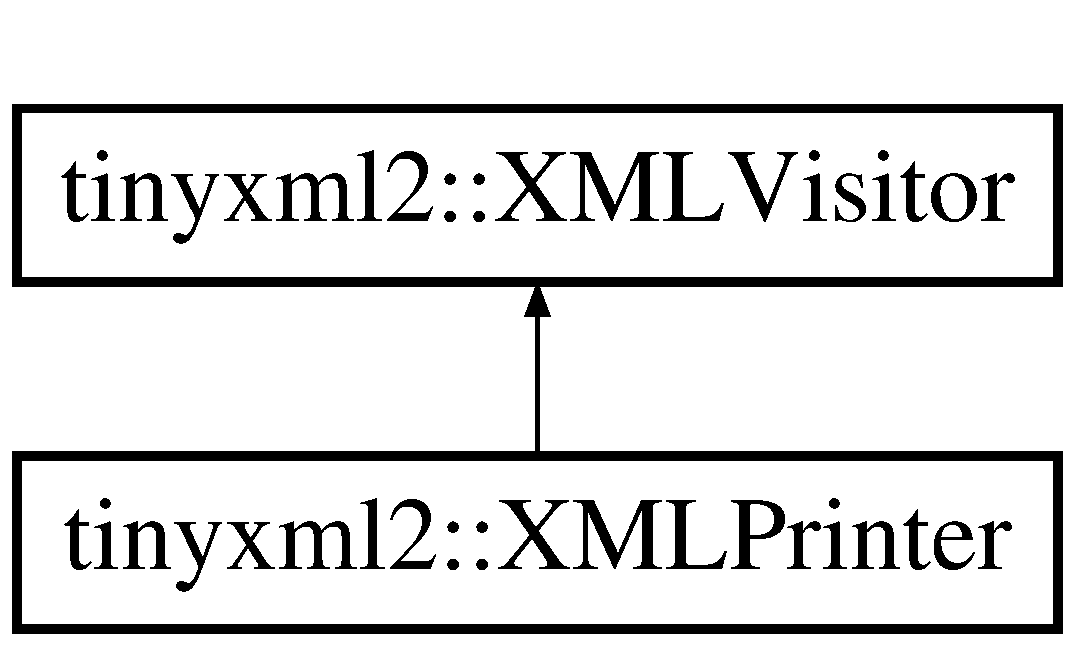
\includegraphics[height=2.000000cm]{classtinyxml2_1_1_x_m_l_printer}
\end{center}
\end{figure}
\subsection*{Public Member Functions}
\begin{DoxyCompactItemize}
\item 
\hyperlink{classtinyxml2_1_1_x_m_l_printer_aa6d3841c069085f5b8a27bc7103c04f7}{X\-M\-L\-Printer} (F\-I\-L\-E $\ast$file=0, bool compact=false, int depth=0)
\item 
\hyperlink{classtinyxml2_1_1_x_m_l_printer_a6de4c23a2941bd738a97b2bfd0000514}{$\sim$\-X\-M\-L\-Printer} ()
\item 
void \hyperlink{classtinyxml2_1_1_x_m_l_printer_a178c608ce8476043d5d6513819cde903}{Push\-Header} (bool write\-B\-O\-M, bool write\-Declaration)
\item 
void \hyperlink{classtinyxml2_1_1_x_m_l_printer_aa10d330818dbc31b44e9ffc27618bdfb}{Open\-Element} (const char $\ast$name)
\item 
void \hyperlink{classtinyxml2_1_1_x_m_l_printer_a9a4e2c9348b42e147629d5a99f4af3f0}{Push\-Attribute} (const char $\ast$name, const char $\ast$value)
\begin{DoxyCompactList}\small\item\em If streaming, add an attribute to an open element. \end{DoxyCompactList}\item 
void \hyperlink{classtinyxml2_1_1_x_m_l_printer_a69120c82088597372d28d0a98f2ee7a1}{Push\-Attribute} (const char $\ast$name, int value)
\item 
void \hyperlink{classtinyxml2_1_1_x_m_l_printer_aa41039e51990aaf5342f3e0575a692c4}{Push\-Attribute} (const char $\ast$name, unsigned value)
\item 
void \hyperlink{classtinyxml2_1_1_x_m_l_printer_a51f7950d7b7a19f0d3a0d549a318d45f}{Push\-Attribute} (const char $\ast$name, bool value)
\item 
void \hyperlink{classtinyxml2_1_1_x_m_l_printer_a1714867af40e68ca404c3e84b6cac2a6}{Push\-Attribute} (const char $\ast$name, double value)
\item 
void \hyperlink{classtinyxml2_1_1_x_m_l_printer_aed6cce4bd414a78b3e2a824803c3ec42}{Close\-Element} ()
\begin{DoxyCompactList}\small\item\em If streaming, close the Element. \end{DoxyCompactList}\item 
void \hyperlink{classtinyxml2_1_1_x_m_l_printer_a1cc16a9362df4332012cb13cff6441b3}{Push\-Text} (const char $\ast$text, bool cdata=false)
\begin{DoxyCompactList}\small\item\em Add a text node. \end{DoxyCompactList}\item 
void \hyperlink{classtinyxml2_1_1_x_m_l_printer_a3e0d4d78de25d4cf081009e1431cea7e}{Push\-Text} (int value)
\begin{DoxyCompactList}\small\item\em Add a text node from an integer. \end{DoxyCompactList}\item 
void \hyperlink{classtinyxml2_1_1_x_m_l_printer_a661fb50e7e0a4918d2d259cb0fae647e}{Push\-Text} (unsigned value)
\begin{DoxyCompactList}\small\item\em Add a text node from an unsigned. \end{DoxyCompactList}\item 
void \hyperlink{classtinyxml2_1_1_x_m_l_printer_a4390e5fa1ed05189a8686647345ab29f}{Push\-Text} (bool value)
\begin{DoxyCompactList}\small\item\em Add a text node from a bool. \end{DoxyCompactList}\item 
void \hyperlink{classtinyxml2_1_1_x_m_l_printer_a1dbb1390e829d0673af66b9cd1928bd7}{Push\-Text} (float value)
\begin{DoxyCompactList}\small\item\em Add a text node from a float. \end{DoxyCompactList}\item 
void \hyperlink{classtinyxml2_1_1_x_m_l_printer_aa715302dfc09473c77c853cbd5431965}{Push\-Text} (double value)
\begin{DoxyCompactList}\small\item\em Add a text node from a double. \end{DoxyCompactList}\item 
void \hyperlink{classtinyxml2_1_1_x_m_l_printer_afc8416814219591c2fd5656e0c233140}{Push\-Comment} (const char $\ast$comment)
\begin{DoxyCompactList}\small\item\em Add a comment. \end{DoxyCompactList}\item 
void \hyperlink{classtinyxml2_1_1_x_m_l_printer_a2fe3565e262594efc6c0276723c83fe7}{Push\-Declaration} (const char $\ast$value)
\item 
void \hyperlink{classtinyxml2_1_1_x_m_l_printer_ab1efc6d1548505e9984185f58f54b713}{Push\-Unknown} (const char $\ast$value)
\item 
virtual bool \hyperlink{classtinyxml2_1_1_x_m_l_printer_a9aa1de11a55a07db55a90fde37d7afad}{Visit\-Enter} (const \hyperlink{classtinyxml2_1_1_x_m_l_document}{X\-M\-L\-Document} \&)
\begin{DoxyCompactList}\small\item\em Visit a document. \end{DoxyCompactList}\item 
virtual bool \hyperlink{classtinyxml2_1_1_x_m_l_printer_a15fc1f2b922f540917dcf52808737b29}{Visit\-Exit} (const \hyperlink{classtinyxml2_1_1_x_m_l_document}{X\-M\-L\-Document} \&)
\begin{DoxyCompactList}\small\item\em Visit a document. \end{DoxyCompactList}\item 
virtual bool \hyperlink{classtinyxml2_1_1_x_m_l_printer_a169b2509d8eabb70811b2bb8cfd1f5d1}{Visit\-Enter} (const \hyperlink{classtinyxml2_1_1_x_m_l_element}{X\-M\-L\-Element} \&element, const \hyperlink{classtinyxml2_1_1_x_m_l_attribute}{X\-M\-L\-Attribute} $\ast$attribute)
\begin{DoxyCompactList}\small\item\em Visit an element. \end{DoxyCompactList}\item 
virtual bool \hyperlink{classtinyxml2_1_1_x_m_l_printer_a2edd48405971a88951c71c9df86a2f50}{Visit\-Exit} (const \hyperlink{classtinyxml2_1_1_x_m_l_element}{X\-M\-L\-Element} \&element)
\begin{DoxyCompactList}\small\item\em Visit an element. \end{DoxyCompactList}\item 
virtual bool \hyperlink{classtinyxml2_1_1_x_m_l_printer_adc0e42b4f6fcb90a95630c79575d030b}{Visit} (const \hyperlink{classtinyxml2_1_1_x_m_l_text}{X\-M\-L\-Text} \&text)
\begin{DoxyCompactList}\small\item\em Visit a text node. \end{DoxyCompactList}\item 
virtual bool \hyperlink{classtinyxml2_1_1_x_m_l_printer_aa294c5c01af0ebb9114902456e4cb53c}{Visit} (const \hyperlink{classtinyxml2_1_1_x_m_l_comment}{X\-M\-L\-Comment} \&comment)
\begin{DoxyCompactList}\small\item\em Visit a comment node. \end{DoxyCompactList}\item 
virtual bool \hyperlink{classtinyxml2_1_1_x_m_l_printer_acfc625b2549304b9c7eb85ebd5c5eb39}{Visit} (const \hyperlink{classtinyxml2_1_1_x_m_l_declaration}{X\-M\-L\-Declaration} \&declaration)
\begin{DoxyCompactList}\small\item\em Visit a declaration. \end{DoxyCompactList}\item 
virtual bool \hyperlink{classtinyxml2_1_1_x_m_l_printer_ab8af5455bbf9e4be2663e6642fcd7e32}{Visit} (const \hyperlink{classtinyxml2_1_1_x_m_l_unknown}{X\-M\-L\-Unknown} \&unknown)
\begin{DoxyCompactList}\small\item\em Visit an unknown node. \end{DoxyCompactList}\item 
const char $\ast$ \hyperlink{classtinyxml2_1_1_x_m_l_printer_a4a1b788e11b540921ec50687cd2b24a9}{C\-Str} () const 
\item 
int \hyperlink{classtinyxml2_1_1_x_m_l_printer_a02c3c5f8c6c007dcbaf10595d9e22bf0}{C\-Str\-Size} () const 
\end{DoxyCompactItemize}


\subsection{Detailed Description}
Printing functionality. The \hyperlink{classtinyxml2_1_1_x_m_l_printer}{X\-M\-L\-Printer} gives you more options than the \hyperlink{classtinyxml2_1_1_x_m_l_document_a686ea28672c0e0c60383ec28148c1ac0}{X\-M\-L\-Document\-::\-Print()} method.

It can\-:
\begin{DoxyEnumerate}
\item Print to memory.
\item Print to a file you provide.
\item Print \hyperlink{namespace_x_m_l}{X\-M\-L} without a \hyperlink{classtinyxml2_1_1_x_m_l_document}{X\-M\-L\-Document}.
\end{DoxyEnumerate}

Print to Memory

\begin{DoxyVerb}XMLPrinter printer;
doc.Print( &printer );
SomeFunction( printer.CStr() );
\end{DoxyVerb}


Print to a File

You provide the file pointer. \begin{DoxyVerb}XMLPrinter printer( fp );
doc.Print( &printer );
\end{DoxyVerb}


Print without a \hyperlink{classtinyxml2_1_1_x_m_l_document}{X\-M\-L\-Document}

When loading, an \hyperlink{namespace_x_m_l}{X\-M\-L} parser is very useful. However, sometimes when saving, it just gets in the way. The code is often set up for streaming, and constructing the D\-O\-M is just overhead.

The Printer supports the streaming case. The following code prints out a trivially simple \hyperlink{namespace_x_m_l}{X\-M\-L} file without ever creating an \hyperlink{namespace_x_m_l}{X\-M\-L} document.

\begin{DoxyVerb}XMLPrinter printer( fp );
printer.OpenElement( "foo" );
printer.PushAttribute( "foo", "bar" );
printer.CloseElement();
\end{DoxyVerb}
 

Definition at line 1877 of file tinyxml2.\-hpp.



\subsection{Constructor \& Destructor Documentation}
\hypertarget{classtinyxml2_1_1_x_m_l_printer_aa6d3841c069085f5b8a27bc7103c04f7}{\index{tinyxml2\-::\-X\-M\-L\-Printer@{tinyxml2\-::\-X\-M\-L\-Printer}!X\-M\-L\-Printer@{X\-M\-L\-Printer}}
\index{X\-M\-L\-Printer@{X\-M\-L\-Printer}!tinyxml2::XMLPrinter@{tinyxml2\-::\-X\-M\-L\-Printer}}
\subsubsection[{X\-M\-L\-Printer}]{\setlength{\rightskip}{0pt plus 5cm}tinyxml2\-::\-X\-M\-L\-Printer\-::\-X\-M\-L\-Printer (
\begin{DoxyParamCaption}
\item[{F\-I\-L\-E $\ast$}]{file = {\ttfamily 0}, }
\item[{bool}]{compact = {\ttfamily false}, }
\item[{int}]{depth = {\ttfamily 0}}
\end{DoxyParamCaption}
)}}\label{classtinyxml2_1_1_x_m_l_printer_aa6d3841c069085f5b8a27bc7103c04f7}
Construct the printer. If the F\-I\-L\-E$\ast$ is specified, this will print to the F\-I\-L\-E. Else it will print to memory, and the result is available in \hyperlink{classtinyxml2_1_1_x_m_l_printer_a4a1b788e11b540921ec50687cd2b24a9}{C\-Str()}. If 'compact' is set to true, then output is created with only required whitespace and newlines. 

Definition at line 1732 of file tinyxml2.\-cpp.

\hypertarget{classtinyxml2_1_1_x_m_l_printer_a6de4c23a2941bd738a97b2bfd0000514}{\index{tinyxml2\-::\-X\-M\-L\-Printer@{tinyxml2\-::\-X\-M\-L\-Printer}!$\sim$\-X\-M\-L\-Printer@{$\sim$\-X\-M\-L\-Printer}}
\index{$\sim$\-X\-M\-L\-Printer@{$\sim$\-X\-M\-L\-Printer}!tinyxml2::XMLPrinter@{tinyxml2\-::\-X\-M\-L\-Printer}}
\subsubsection[{$\sim$\-X\-M\-L\-Printer}]{\setlength{\rightskip}{0pt plus 5cm}tinyxml2\-::\-X\-M\-L\-Printer\-::$\sim$\-X\-M\-L\-Printer (
\begin{DoxyParamCaption}
{}
\end{DoxyParamCaption}
)\hspace{0.3cm}{\ttfamily [inline]}}}\label{classtinyxml2_1_1_x_m_l_printer_a6de4c23a2941bd738a97b2bfd0000514}


Definition at line 1887 of file tinyxml2.\-hpp.



\subsection{Member Function Documentation}
\hypertarget{classtinyxml2_1_1_x_m_l_printer_aed6cce4bd414a78b3e2a824803c3ec42}{\index{tinyxml2\-::\-X\-M\-L\-Printer@{tinyxml2\-::\-X\-M\-L\-Printer}!Close\-Element@{Close\-Element}}
\index{Close\-Element@{Close\-Element}!tinyxml2::XMLPrinter@{tinyxml2\-::\-X\-M\-L\-Printer}}
\subsubsection[{Close\-Element}]{\setlength{\rightskip}{0pt plus 5cm}void tinyxml2\-::\-X\-M\-L\-Printer\-::\-Close\-Element (
\begin{DoxyParamCaption}
{}
\end{DoxyParamCaption}
)}}\label{classtinyxml2_1_1_x_m_l_printer_aed6cce4bd414a78b3e2a824803c3ec42}


If streaming, close the Element. 



Definition at line 1914 of file tinyxml2.\-cpp.

\hypertarget{classtinyxml2_1_1_x_m_l_printer_a4a1b788e11b540921ec50687cd2b24a9}{\index{tinyxml2\-::\-X\-M\-L\-Printer@{tinyxml2\-::\-X\-M\-L\-Printer}!C\-Str@{C\-Str}}
\index{C\-Str@{C\-Str}!tinyxml2::XMLPrinter@{tinyxml2\-::\-X\-M\-L\-Printer}}
\subsubsection[{C\-Str}]{\setlength{\rightskip}{0pt plus 5cm}const char$\ast$ tinyxml2\-::\-X\-M\-L\-Printer\-::\-C\-Str (
\begin{DoxyParamCaption}
{}
\end{DoxyParamCaption}
) const\hspace{0.3cm}{\ttfamily [inline]}}}\label{classtinyxml2_1_1_x_m_l_printer_a4a1b788e11b540921ec50687cd2b24a9}
If in print to memory mode, return a pointer to the \hyperlink{namespace_x_m_l}{X\-M\-L} file in memory. 

Definition at line 1940 of file tinyxml2.\-hpp.

\hypertarget{classtinyxml2_1_1_x_m_l_printer_a02c3c5f8c6c007dcbaf10595d9e22bf0}{\index{tinyxml2\-::\-X\-M\-L\-Printer@{tinyxml2\-::\-X\-M\-L\-Printer}!C\-Str\-Size@{C\-Str\-Size}}
\index{C\-Str\-Size@{C\-Str\-Size}!tinyxml2::XMLPrinter@{tinyxml2\-::\-X\-M\-L\-Printer}}
\subsubsection[{C\-Str\-Size}]{\setlength{\rightskip}{0pt plus 5cm}int tinyxml2\-::\-X\-M\-L\-Printer\-::\-C\-Str\-Size (
\begin{DoxyParamCaption}
{}
\end{DoxyParamCaption}
) const\hspace{0.3cm}{\ttfamily [inline]}}}\label{classtinyxml2_1_1_x_m_l_printer_a02c3c5f8c6c007dcbaf10595d9e22bf0}
If in print to memory mode, return the size of the \hyperlink{namespace_x_m_l}{X\-M\-L} file in memory. (Note the size returned includes the terminating null.) 

Definition at line 1948 of file tinyxml2.\-hpp.

\hypertarget{classtinyxml2_1_1_x_m_l_printer_aa10d330818dbc31b44e9ffc27618bdfb}{\index{tinyxml2\-::\-X\-M\-L\-Printer@{tinyxml2\-::\-X\-M\-L\-Printer}!Open\-Element@{Open\-Element}}
\index{Open\-Element@{Open\-Element}!tinyxml2::XMLPrinter@{tinyxml2\-::\-X\-M\-L\-Printer}}
\subsubsection[{Open\-Element}]{\setlength{\rightskip}{0pt plus 5cm}void tinyxml2\-::\-X\-M\-L\-Printer\-::\-Open\-Element (
\begin{DoxyParamCaption}
\item[{const char $\ast$}]{name}
\end{DoxyParamCaption}
)}}\label{classtinyxml2_1_1_x_m_l_printer_aa10d330818dbc31b44e9ffc27618bdfb}
If streaming, start writing an element. The element must be closed with \hyperlink{classtinyxml2_1_1_x_m_l_printer_aed6cce4bd414a78b3e2a824803c3ec42}{Close\-Element()} 

Definition at line 1852 of file tinyxml2.\-cpp.

\hypertarget{classtinyxml2_1_1_x_m_l_printer_a9a4e2c9348b42e147629d5a99f4af3f0}{\index{tinyxml2\-::\-X\-M\-L\-Printer@{tinyxml2\-::\-X\-M\-L\-Printer}!Push\-Attribute@{Push\-Attribute}}
\index{Push\-Attribute@{Push\-Attribute}!tinyxml2::XMLPrinter@{tinyxml2\-::\-X\-M\-L\-Printer}}
\subsubsection[{Push\-Attribute}]{\setlength{\rightskip}{0pt plus 5cm}void tinyxml2\-::\-X\-M\-L\-Printer\-::\-Push\-Attribute (
\begin{DoxyParamCaption}
\item[{const char $\ast$}]{name, }
\item[{const char $\ast$}]{value}
\end{DoxyParamCaption}
)}}\label{classtinyxml2_1_1_x_m_l_printer_a9a4e2c9348b42e147629d5a99f4af3f0}


If streaming, add an attribute to an open element. 



Definition at line 1873 of file tinyxml2.\-cpp.

\hypertarget{classtinyxml2_1_1_x_m_l_printer_a69120c82088597372d28d0a98f2ee7a1}{\index{tinyxml2\-::\-X\-M\-L\-Printer@{tinyxml2\-::\-X\-M\-L\-Printer}!Push\-Attribute@{Push\-Attribute}}
\index{Push\-Attribute@{Push\-Attribute}!tinyxml2::XMLPrinter@{tinyxml2\-::\-X\-M\-L\-Printer}}
\subsubsection[{Push\-Attribute}]{\setlength{\rightskip}{0pt plus 5cm}void tinyxml2\-::\-X\-M\-L\-Printer\-::\-Push\-Attribute (
\begin{DoxyParamCaption}
\item[{const char $\ast$}]{name, }
\item[{int}]{value}
\end{DoxyParamCaption}
)}}\label{classtinyxml2_1_1_x_m_l_printer_a69120c82088597372d28d0a98f2ee7a1}


Definition at line 1882 of file tinyxml2.\-cpp.

\hypertarget{classtinyxml2_1_1_x_m_l_printer_aa41039e51990aaf5342f3e0575a692c4}{\index{tinyxml2\-::\-X\-M\-L\-Printer@{tinyxml2\-::\-X\-M\-L\-Printer}!Push\-Attribute@{Push\-Attribute}}
\index{Push\-Attribute@{Push\-Attribute}!tinyxml2::XMLPrinter@{tinyxml2\-::\-X\-M\-L\-Printer}}
\subsubsection[{Push\-Attribute}]{\setlength{\rightskip}{0pt plus 5cm}void tinyxml2\-::\-X\-M\-L\-Printer\-::\-Push\-Attribute (
\begin{DoxyParamCaption}
\item[{const char $\ast$}]{name, }
\item[{unsigned}]{value}
\end{DoxyParamCaption}
)}}\label{classtinyxml2_1_1_x_m_l_printer_aa41039e51990aaf5342f3e0575a692c4}


Definition at line 1890 of file tinyxml2.\-cpp.

\hypertarget{classtinyxml2_1_1_x_m_l_printer_a51f7950d7b7a19f0d3a0d549a318d45f}{\index{tinyxml2\-::\-X\-M\-L\-Printer@{tinyxml2\-::\-X\-M\-L\-Printer}!Push\-Attribute@{Push\-Attribute}}
\index{Push\-Attribute@{Push\-Attribute}!tinyxml2::XMLPrinter@{tinyxml2\-::\-X\-M\-L\-Printer}}
\subsubsection[{Push\-Attribute}]{\setlength{\rightskip}{0pt plus 5cm}void tinyxml2\-::\-X\-M\-L\-Printer\-::\-Push\-Attribute (
\begin{DoxyParamCaption}
\item[{const char $\ast$}]{name, }
\item[{bool}]{value}
\end{DoxyParamCaption}
)}}\label{classtinyxml2_1_1_x_m_l_printer_a51f7950d7b7a19f0d3a0d549a318d45f}


Definition at line 1898 of file tinyxml2.\-cpp.

\hypertarget{classtinyxml2_1_1_x_m_l_printer_a1714867af40e68ca404c3e84b6cac2a6}{\index{tinyxml2\-::\-X\-M\-L\-Printer@{tinyxml2\-::\-X\-M\-L\-Printer}!Push\-Attribute@{Push\-Attribute}}
\index{Push\-Attribute@{Push\-Attribute}!tinyxml2::XMLPrinter@{tinyxml2\-::\-X\-M\-L\-Printer}}
\subsubsection[{Push\-Attribute}]{\setlength{\rightskip}{0pt plus 5cm}void tinyxml2\-::\-X\-M\-L\-Printer\-::\-Push\-Attribute (
\begin{DoxyParamCaption}
\item[{const char $\ast$}]{name, }
\item[{double}]{value}
\end{DoxyParamCaption}
)}}\label{classtinyxml2_1_1_x_m_l_printer_a1714867af40e68ca404c3e84b6cac2a6}


Definition at line 1906 of file tinyxml2.\-cpp.

\hypertarget{classtinyxml2_1_1_x_m_l_printer_afc8416814219591c2fd5656e0c233140}{\index{tinyxml2\-::\-X\-M\-L\-Printer@{tinyxml2\-::\-X\-M\-L\-Printer}!Push\-Comment@{Push\-Comment}}
\index{Push\-Comment@{Push\-Comment}!tinyxml2::XMLPrinter@{tinyxml2\-::\-X\-M\-L\-Printer}}
\subsubsection[{Push\-Comment}]{\setlength{\rightskip}{0pt plus 5cm}void tinyxml2\-::\-X\-M\-L\-Printer\-::\-Push\-Comment (
\begin{DoxyParamCaption}
\item[{const char $\ast$}]{comment}
\end{DoxyParamCaption}
)}}\label{classtinyxml2_1_1_x_m_l_printer_afc8416814219591c2fd5656e0c233140}


Add a comment. 



Definition at line 2004 of file tinyxml2.\-cpp.

\hypertarget{classtinyxml2_1_1_x_m_l_printer_a2fe3565e262594efc6c0276723c83fe7}{\index{tinyxml2\-::\-X\-M\-L\-Printer@{tinyxml2\-::\-X\-M\-L\-Printer}!Push\-Declaration@{Push\-Declaration}}
\index{Push\-Declaration@{Push\-Declaration}!tinyxml2::XMLPrinter@{tinyxml2\-::\-X\-M\-L\-Printer}}
\subsubsection[{Push\-Declaration}]{\setlength{\rightskip}{0pt plus 5cm}void tinyxml2\-::\-X\-M\-L\-Printer\-::\-Push\-Declaration (
\begin{DoxyParamCaption}
\item[{const char $\ast$}]{value}
\end{DoxyParamCaption}
)}}\label{classtinyxml2_1_1_x_m_l_printer_a2fe3565e262594efc6c0276723c83fe7}


Definition at line 2018 of file tinyxml2.\-cpp.

\hypertarget{classtinyxml2_1_1_x_m_l_printer_a178c608ce8476043d5d6513819cde903}{\index{tinyxml2\-::\-X\-M\-L\-Printer@{tinyxml2\-::\-X\-M\-L\-Printer}!Push\-Header@{Push\-Header}}
\index{Push\-Header@{Push\-Header}!tinyxml2::XMLPrinter@{tinyxml2\-::\-X\-M\-L\-Printer}}
\subsubsection[{Push\-Header}]{\setlength{\rightskip}{0pt plus 5cm}void tinyxml2\-::\-X\-M\-L\-Printer\-::\-Push\-Header (
\begin{DoxyParamCaption}
\item[{bool}]{write\-B\-O\-M, }
\item[{bool}]{write\-Declaration}
\end{DoxyParamCaption}
)}}\label{classtinyxml2_1_1_x_m_l_printer_a178c608ce8476043d5d6513819cde903}
If streaming, write the B\-O\-M and declaration. 

Definition at line 1840 of file tinyxml2.\-cpp.

\hypertarget{classtinyxml2_1_1_x_m_l_printer_a1cc16a9362df4332012cb13cff6441b3}{\index{tinyxml2\-::\-X\-M\-L\-Printer@{tinyxml2\-::\-X\-M\-L\-Printer}!Push\-Text@{Push\-Text}}
\index{Push\-Text@{Push\-Text}!tinyxml2::XMLPrinter@{tinyxml2\-::\-X\-M\-L\-Printer}}
\subsubsection[{Push\-Text}]{\setlength{\rightskip}{0pt plus 5cm}void tinyxml2\-::\-X\-M\-L\-Printer\-::\-Push\-Text (
\begin{DoxyParamCaption}
\item[{const char $\ast$}]{text, }
\item[{bool}]{cdata = {\ttfamily false}}
\end{DoxyParamCaption}
)}}\label{classtinyxml2_1_1_x_m_l_printer_a1cc16a9362df4332012cb13cff6441b3}


Add a text node. 



Definition at line 1947 of file tinyxml2.\-cpp.

\hypertarget{classtinyxml2_1_1_x_m_l_printer_a3e0d4d78de25d4cf081009e1431cea7e}{\index{tinyxml2\-::\-X\-M\-L\-Printer@{tinyxml2\-::\-X\-M\-L\-Printer}!Push\-Text@{Push\-Text}}
\index{Push\-Text@{Push\-Text}!tinyxml2::XMLPrinter@{tinyxml2\-::\-X\-M\-L\-Printer}}
\subsubsection[{Push\-Text}]{\setlength{\rightskip}{0pt plus 5cm}void tinyxml2\-::\-X\-M\-L\-Printer\-::\-Push\-Text (
\begin{DoxyParamCaption}
\item[{int}]{value}
\end{DoxyParamCaption}
)}}\label{classtinyxml2_1_1_x_m_l_printer_a3e0d4d78de25d4cf081009e1431cea7e}


Add a text node from an integer. 



Definition at line 1964 of file tinyxml2.\-cpp.

\hypertarget{classtinyxml2_1_1_x_m_l_printer_a661fb50e7e0a4918d2d259cb0fae647e}{\index{tinyxml2\-::\-X\-M\-L\-Printer@{tinyxml2\-::\-X\-M\-L\-Printer}!Push\-Text@{Push\-Text}}
\index{Push\-Text@{Push\-Text}!tinyxml2::XMLPrinter@{tinyxml2\-::\-X\-M\-L\-Printer}}
\subsubsection[{Push\-Text}]{\setlength{\rightskip}{0pt plus 5cm}void tinyxml2\-::\-X\-M\-L\-Printer\-::\-Push\-Text (
\begin{DoxyParamCaption}
\item[{unsigned}]{value}
\end{DoxyParamCaption}
)}}\label{classtinyxml2_1_1_x_m_l_printer_a661fb50e7e0a4918d2d259cb0fae647e}


Add a text node from an unsigned. 



Definition at line 1972 of file tinyxml2.\-cpp.

\hypertarget{classtinyxml2_1_1_x_m_l_printer_a4390e5fa1ed05189a8686647345ab29f}{\index{tinyxml2\-::\-X\-M\-L\-Printer@{tinyxml2\-::\-X\-M\-L\-Printer}!Push\-Text@{Push\-Text}}
\index{Push\-Text@{Push\-Text}!tinyxml2::XMLPrinter@{tinyxml2\-::\-X\-M\-L\-Printer}}
\subsubsection[{Push\-Text}]{\setlength{\rightskip}{0pt plus 5cm}void tinyxml2\-::\-X\-M\-L\-Printer\-::\-Push\-Text (
\begin{DoxyParamCaption}
\item[{bool}]{value}
\end{DoxyParamCaption}
)}}\label{classtinyxml2_1_1_x_m_l_printer_a4390e5fa1ed05189a8686647345ab29f}


Add a text node from a bool. 



Definition at line 1980 of file tinyxml2.\-cpp.

\hypertarget{classtinyxml2_1_1_x_m_l_printer_a1dbb1390e829d0673af66b9cd1928bd7}{\index{tinyxml2\-::\-X\-M\-L\-Printer@{tinyxml2\-::\-X\-M\-L\-Printer}!Push\-Text@{Push\-Text}}
\index{Push\-Text@{Push\-Text}!tinyxml2::XMLPrinter@{tinyxml2\-::\-X\-M\-L\-Printer}}
\subsubsection[{Push\-Text}]{\setlength{\rightskip}{0pt plus 5cm}void tinyxml2\-::\-X\-M\-L\-Printer\-::\-Push\-Text (
\begin{DoxyParamCaption}
\item[{float}]{value}
\end{DoxyParamCaption}
)}}\label{classtinyxml2_1_1_x_m_l_printer_a1dbb1390e829d0673af66b9cd1928bd7}


Add a text node from a float. 



Definition at line 1988 of file tinyxml2.\-cpp.

\hypertarget{classtinyxml2_1_1_x_m_l_printer_aa715302dfc09473c77c853cbd5431965}{\index{tinyxml2\-::\-X\-M\-L\-Printer@{tinyxml2\-::\-X\-M\-L\-Printer}!Push\-Text@{Push\-Text}}
\index{Push\-Text@{Push\-Text}!tinyxml2::XMLPrinter@{tinyxml2\-::\-X\-M\-L\-Printer}}
\subsubsection[{Push\-Text}]{\setlength{\rightskip}{0pt plus 5cm}void tinyxml2\-::\-X\-M\-L\-Printer\-::\-Push\-Text (
\begin{DoxyParamCaption}
\item[{double}]{value}
\end{DoxyParamCaption}
)}}\label{classtinyxml2_1_1_x_m_l_printer_aa715302dfc09473c77c853cbd5431965}


Add a text node from a double. 



Definition at line 1996 of file tinyxml2.\-cpp.

\hypertarget{classtinyxml2_1_1_x_m_l_printer_ab1efc6d1548505e9984185f58f54b713}{\index{tinyxml2\-::\-X\-M\-L\-Printer@{tinyxml2\-::\-X\-M\-L\-Printer}!Push\-Unknown@{Push\-Unknown}}
\index{Push\-Unknown@{Push\-Unknown}!tinyxml2::XMLPrinter@{tinyxml2\-::\-X\-M\-L\-Printer}}
\subsubsection[{Push\-Unknown}]{\setlength{\rightskip}{0pt plus 5cm}void tinyxml2\-::\-X\-M\-L\-Printer\-::\-Push\-Unknown (
\begin{DoxyParamCaption}
\item[{const char $\ast$}]{value}
\end{DoxyParamCaption}
)}}\label{classtinyxml2_1_1_x_m_l_printer_ab1efc6d1548505e9984185f58f54b713}


Definition at line 2032 of file tinyxml2.\-cpp.

\hypertarget{classtinyxml2_1_1_x_m_l_printer_adc0e42b4f6fcb90a95630c79575d030b}{\index{tinyxml2\-::\-X\-M\-L\-Printer@{tinyxml2\-::\-X\-M\-L\-Printer}!Visit@{Visit}}
\index{Visit@{Visit}!tinyxml2::XMLPrinter@{tinyxml2\-::\-X\-M\-L\-Printer}}
\subsubsection[{Visit}]{\setlength{\rightskip}{0pt plus 5cm}bool tinyxml2\-::\-X\-M\-L\-Printer\-::\-Visit (
\begin{DoxyParamCaption}
\item[{const {\bf X\-M\-L\-Text} \&}]{}
\end{DoxyParamCaption}
)\hspace{0.3cm}{\ttfamily [virtual]}}}\label{classtinyxml2_1_1_x_m_l_printer_adc0e42b4f6fcb90a95630c79575d030b}


Visit a text node. 



Reimplemented from \hyperlink{classtinyxml2_1_1_x_m_l_visitor_af30233565856480ea48b6fa0d6dec65b}{tinyxml2\-::\-X\-M\-L\-Visitor}.



Definition at line 2074 of file tinyxml2.\-cpp.

\hypertarget{classtinyxml2_1_1_x_m_l_printer_aa294c5c01af0ebb9114902456e4cb53c}{\index{tinyxml2\-::\-X\-M\-L\-Printer@{tinyxml2\-::\-X\-M\-L\-Printer}!Visit@{Visit}}
\index{Visit@{Visit}!tinyxml2::XMLPrinter@{tinyxml2\-::\-X\-M\-L\-Printer}}
\subsubsection[{Visit}]{\setlength{\rightskip}{0pt plus 5cm}bool tinyxml2\-::\-X\-M\-L\-Printer\-::\-Visit (
\begin{DoxyParamCaption}
\item[{const {\bf X\-M\-L\-Comment} \&}]{}
\end{DoxyParamCaption}
)\hspace{0.3cm}{\ttfamily [virtual]}}}\label{classtinyxml2_1_1_x_m_l_printer_aa294c5c01af0ebb9114902456e4cb53c}


Visit a comment node. 



Reimplemented from \hyperlink{classtinyxml2_1_1_x_m_l_visitor_acc8147fb5a85f6c65721654e427752d7}{tinyxml2\-::\-X\-M\-L\-Visitor}.



Definition at line 2081 of file tinyxml2.\-cpp.

\hypertarget{classtinyxml2_1_1_x_m_l_printer_acfc625b2549304b9c7eb85ebd5c5eb39}{\index{tinyxml2\-::\-X\-M\-L\-Printer@{tinyxml2\-::\-X\-M\-L\-Printer}!Visit@{Visit}}
\index{Visit@{Visit}!tinyxml2::XMLPrinter@{tinyxml2\-::\-X\-M\-L\-Printer}}
\subsubsection[{Visit}]{\setlength{\rightskip}{0pt plus 5cm}bool tinyxml2\-::\-X\-M\-L\-Printer\-::\-Visit (
\begin{DoxyParamCaption}
\item[{const {\bf X\-M\-L\-Declaration} \&}]{}
\end{DoxyParamCaption}
)\hspace{0.3cm}{\ttfamily [virtual]}}}\label{classtinyxml2_1_1_x_m_l_printer_acfc625b2549304b9c7eb85ebd5c5eb39}


Visit a declaration. 



Reimplemented from \hyperlink{classtinyxml2_1_1_x_m_l_visitor_adc75bd459fc7ba8223b50f0616767f9a}{tinyxml2\-::\-X\-M\-L\-Visitor}.



Definition at line 2087 of file tinyxml2.\-cpp.

\hypertarget{classtinyxml2_1_1_x_m_l_printer_ab8af5455bbf9e4be2663e6642fcd7e32}{\index{tinyxml2\-::\-X\-M\-L\-Printer@{tinyxml2\-::\-X\-M\-L\-Printer}!Visit@{Visit}}
\index{Visit@{Visit}!tinyxml2::XMLPrinter@{tinyxml2\-::\-X\-M\-L\-Printer}}
\subsubsection[{Visit}]{\setlength{\rightskip}{0pt plus 5cm}bool tinyxml2\-::\-X\-M\-L\-Printer\-::\-Visit (
\begin{DoxyParamCaption}
\item[{const {\bf X\-M\-L\-Unknown} \&}]{}
\end{DoxyParamCaption}
)\hspace{0.3cm}{\ttfamily [virtual]}}}\label{classtinyxml2_1_1_x_m_l_printer_ab8af5455bbf9e4be2663e6642fcd7e32}


Visit an unknown node. 



Reimplemented from \hyperlink{classtinyxml2_1_1_x_m_l_visitor_a14e4748387c34bf53d24e8119bb1f292}{tinyxml2\-::\-X\-M\-L\-Visitor}.



Definition at line 2094 of file tinyxml2.\-cpp.

\hypertarget{classtinyxml2_1_1_x_m_l_printer_a9aa1de11a55a07db55a90fde37d7afad}{\index{tinyxml2\-::\-X\-M\-L\-Printer@{tinyxml2\-::\-X\-M\-L\-Printer}!Visit\-Enter@{Visit\-Enter}}
\index{Visit\-Enter@{Visit\-Enter}!tinyxml2::XMLPrinter@{tinyxml2\-::\-X\-M\-L\-Printer}}
\subsubsection[{Visit\-Enter}]{\setlength{\rightskip}{0pt plus 5cm}bool tinyxml2\-::\-X\-M\-L\-Printer\-::\-Visit\-Enter (
\begin{DoxyParamCaption}
\item[{const {\bf X\-M\-L\-Document} \&}]{}
\end{DoxyParamCaption}
)\hspace{0.3cm}{\ttfamily [virtual]}}}\label{classtinyxml2_1_1_x_m_l_printer_a9aa1de11a55a07db55a90fde37d7afad}


Visit a document. 



Reimplemented from \hyperlink{classtinyxml2_1_1_x_m_l_visitor_acb3c22fc5f60eb9db98f533f2761f67d}{tinyxml2\-::\-X\-M\-L\-Visitor}.



Definition at line 2046 of file tinyxml2.\-cpp.

\hypertarget{classtinyxml2_1_1_x_m_l_printer_a169b2509d8eabb70811b2bb8cfd1f5d1}{\index{tinyxml2\-::\-X\-M\-L\-Printer@{tinyxml2\-::\-X\-M\-L\-Printer}!Visit\-Enter@{Visit\-Enter}}
\index{Visit\-Enter@{Visit\-Enter}!tinyxml2::XMLPrinter@{tinyxml2\-::\-X\-M\-L\-Printer}}
\subsubsection[{Visit\-Enter}]{\setlength{\rightskip}{0pt plus 5cm}bool tinyxml2\-::\-X\-M\-L\-Printer\-::\-Visit\-Enter (
\begin{DoxyParamCaption}
\item[{const {\bf X\-M\-L\-Element} \&}]{, }
\item[{const {\bf X\-M\-L\-Attribute} $\ast$}]{}
\end{DoxyParamCaption}
)\hspace{0.3cm}{\ttfamily [virtual]}}}\label{classtinyxml2_1_1_x_m_l_printer_a169b2509d8eabb70811b2bb8cfd1f5d1}


Visit an element. 



Reimplemented from \hyperlink{classtinyxml2_1_1_x_m_l_visitor_af97980a17dd4e37448b181f5ddfa92b5}{tinyxml2\-::\-X\-M\-L\-Visitor}.



Definition at line 2056 of file tinyxml2.\-cpp.

\hypertarget{classtinyxml2_1_1_x_m_l_printer_a15fc1f2b922f540917dcf52808737b29}{\index{tinyxml2\-::\-X\-M\-L\-Printer@{tinyxml2\-::\-X\-M\-L\-Printer}!Visit\-Exit@{Visit\-Exit}}
\index{Visit\-Exit@{Visit\-Exit}!tinyxml2::XMLPrinter@{tinyxml2\-::\-X\-M\-L\-Printer}}
\subsubsection[{Visit\-Exit}]{\setlength{\rightskip}{0pt plus 5cm}virtual bool tinyxml2\-::\-X\-M\-L\-Printer\-::\-Visit\-Exit (
\begin{DoxyParamCaption}
\item[{const {\bf X\-M\-L\-Document} \&}]{}
\end{DoxyParamCaption}
)\hspace{0.3cm}{\ttfamily [inline]}, {\ttfamily [virtual]}}}\label{classtinyxml2_1_1_x_m_l_printer_a15fc1f2b922f540917dcf52808737b29}


Visit a document. 



Reimplemented from \hyperlink{classtinyxml2_1_1_x_m_l_visitor_a170e9989cd046ba904f302d087e07086}{tinyxml2\-::\-X\-M\-L\-Visitor}.



Definition at line 1924 of file tinyxml2.\-hpp.

\hypertarget{classtinyxml2_1_1_x_m_l_printer_a2edd48405971a88951c71c9df86a2f50}{\index{tinyxml2\-::\-X\-M\-L\-Printer@{tinyxml2\-::\-X\-M\-L\-Printer}!Visit\-Exit@{Visit\-Exit}}
\index{Visit\-Exit@{Visit\-Exit}!tinyxml2::XMLPrinter@{tinyxml2\-::\-X\-M\-L\-Printer}}
\subsubsection[{Visit\-Exit}]{\setlength{\rightskip}{0pt plus 5cm}bool tinyxml2\-::\-X\-M\-L\-Printer\-::\-Visit\-Exit (
\begin{DoxyParamCaption}
\item[{const {\bf X\-M\-L\-Element} \&}]{}
\end{DoxyParamCaption}
)\hspace{0.3cm}{\ttfamily [virtual]}}}\label{classtinyxml2_1_1_x_m_l_printer_a2edd48405971a88951c71c9df86a2f50}


Visit an element. 



Reimplemented from \hyperlink{classtinyxml2_1_1_x_m_l_visitor_a772f10ddc83f881956d32628faa16eb6}{tinyxml2\-::\-X\-M\-L\-Visitor}.



Definition at line 2067 of file tinyxml2.\-cpp.



The documentation for this class was generated from the following files\-:\begin{DoxyCompactItemize}
\item 
Glide/\hyperlink{tinyxml2_8hpp}{tinyxml2.\-hpp}\item 
Glide/\hyperlink{tinyxml2_8cpp}{tinyxml2.\-cpp}\end{DoxyCompactItemize}

\hypertarget{classtinyxml2_1_1_x_m_l_text}{\section{tinyxml2\-:\-:X\-M\-L\-Text Class Reference}
\label{classtinyxml2_1_1_x_m_l_text}\index{tinyxml2\-::\-X\-M\-L\-Text@{tinyxml2\-::\-X\-M\-L\-Text}}
}


{\ttfamily \#include $<$tinyxml2.\-hpp$>$}

Inheritance diagram for tinyxml2\-:\-:X\-M\-L\-Text\-:\begin{figure}[H]
\begin{center}
\leavevmode
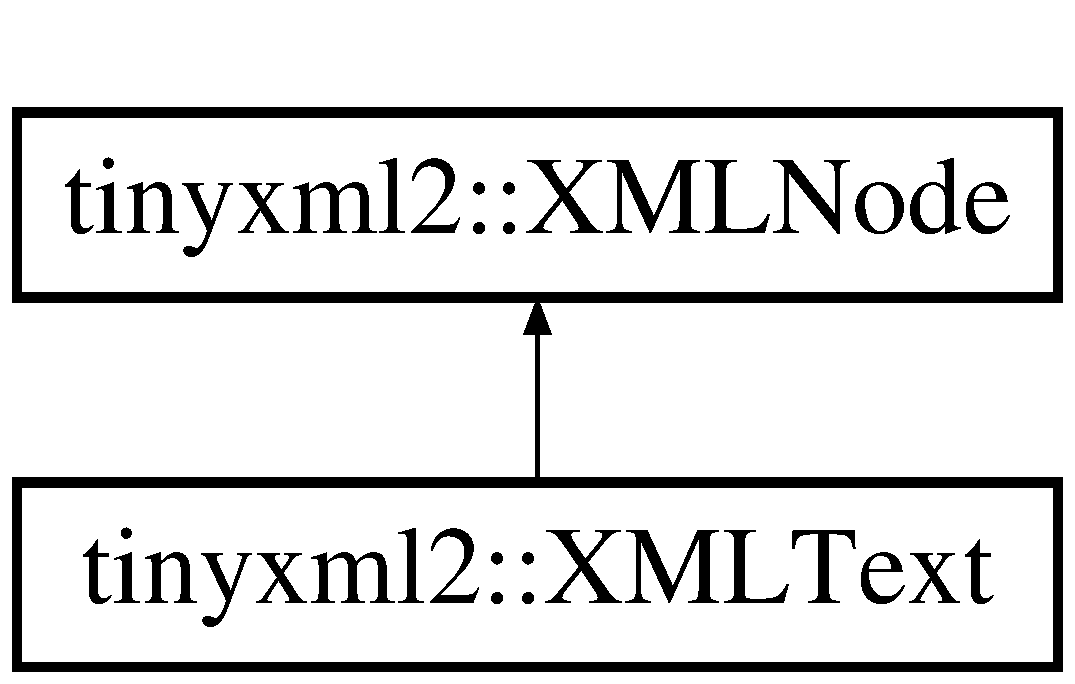
\includegraphics[height=2.000000cm]{classtinyxml2_1_1_x_m_l_text}
\end{center}
\end{figure}
\subsection*{Public Member Functions}
\begin{DoxyCompactItemize}
\item 
virtual bool \hyperlink{classtinyxml2_1_1_x_m_l_text_ae659d4fc7351a7df11c111cbe1ade46f}{Accept} (\hyperlink{classtinyxml2_1_1_x_m_l_visitor}{X\-M\-L\-Visitor} $\ast$visitor) const 
\item 
virtual \hyperlink{classtinyxml2_1_1_x_m_l_text}{X\-M\-L\-Text} $\ast$ \hyperlink{classtinyxml2_1_1_x_m_l_text_ab1213b4ddebe9b17ec7e7040e9f1caf7}{To\-Text} ()
\begin{DoxyCompactList}\small\item\em Safely cast to Text, or null. \end{DoxyCompactList}\item 
virtual const \hyperlink{classtinyxml2_1_1_x_m_l_text}{X\-M\-L\-Text} $\ast$ \hyperlink{classtinyxml2_1_1_x_m_l_text_a1e53cbc60968fe966790a65eaf87baaa}{To\-Text} () const 
\item 
void \hyperlink{classtinyxml2_1_1_x_m_l_text_ad080357d76ab7cc59d7651249949329d}{Set\-C\-Data} (bool is\-C\-Data)
\begin{DoxyCompactList}\small\item\em Declare whether this should be C\-D\-A\-T\-A or standard text. \end{DoxyCompactList}\item 
bool \hyperlink{classtinyxml2_1_1_x_m_l_text_a125574fe49da80efbae1349f20d02d41}{C\-Data} () const 
\begin{DoxyCompactList}\small\item\em Returns true if this is a C\-D\-A\-T\-A text element. \end{DoxyCompactList}\item 
char $\ast$ \hyperlink{classtinyxml2_1_1_x_m_l_text_ac18d9eec9f12b827b0d02b0847bf279e}{Parse\-Deep} (char $\ast$, \hyperlink{classtinyxml2_1_1_str_pair}{Str\-Pair} $\ast$end\-Tag)
\item 
virtual \hyperlink{classtinyxml2_1_1_x_m_l_node}{X\-M\-L\-Node} $\ast$ \hyperlink{classtinyxml2_1_1_x_m_l_text_af5115f8cc83de2947ed6a9d13e2f88c8}{Shallow\-Clone} (\hyperlink{classtinyxml2_1_1_x_m_l_document}{X\-M\-L\-Document} $\ast$document) const 
\item 
virtual bool \hyperlink{classtinyxml2_1_1_x_m_l_text_a1588aa5d23cb21eb31f36df0aaaa8d66}{Shallow\-Equal} (const \hyperlink{classtinyxml2_1_1_x_m_l_node}{X\-M\-L\-Node} $\ast$compare) const 
\end{DoxyCompactItemize}
\subsection*{Protected Member Functions}
\begin{DoxyCompactItemize}
\item 
\hyperlink{classtinyxml2_1_1_x_m_l_text_ad9f46d70e61e5386ead93728d8b90267}{X\-M\-L\-Text} (\hyperlink{classtinyxml2_1_1_x_m_l_document}{X\-M\-L\-Document} $\ast$doc)
\item 
virtual \hyperlink{classtinyxml2_1_1_x_m_l_text_ae9b8790d0dc13914394dbd7437c0e59d}{$\sim$\-X\-M\-L\-Text} ()
\item 
\hyperlink{classtinyxml2_1_1_x_m_l_text_a002156e1f61ee6d48e5368b7cca25582}{X\-M\-L\-Text} (const \hyperlink{classtinyxml2_1_1_x_m_l_text}{X\-M\-L\-Text} \&)
\item 
\hyperlink{classtinyxml2_1_1_x_m_l_text}{X\-M\-L\-Text} \& \hyperlink{classtinyxml2_1_1_x_m_l_text_ad8c9f398d92fa472e213b89d8483ae8f}{operator=} (const \hyperlink{classtinyxml2_1_1_x_m_l_text}{X\-M\-L\-Text} \&)
\end{DoxyCompactItemize}
\subsection*{Friends}
\begin{DoxyCompactItemize}
\item 
class \hyperlink{classtinyxml2_1_1_x_m_l_text_a449202cfc89e7ae5c2f81995476f9ec1}{X\-M\-L\-Base}
\item 
class \hyperlink{classtinyxml2_1_1_x_m_l_text_a4eee3bda60c60a30e4e8cd4ea91c4c6e}{X\-M\-L\-Document}
\end{DoxyCompactItemize}
\subsection*{Additional Inherited Members}


\subsection{Detailed Description}
\hyperlink{namespace_x_m_l}{X\-M\-L} text.

Note that a text node can have child element nodes, for example\-: \begin{DoxyVerb}<root>This is <b>bold</b></root>
\end{DoxyVerb}


A text node can have 2 ways to output the next. \char`\"{}normal\char`\"{} output and C\-D\-A\-T\-A. It will default to the mode it was parsed from the \hyperlink{namespace_x_m_l}{X\-M\-L} file and you generally want to leave it alone, but you can change the output mode with \hyperlink{classtinyxml2_1_1_x_m_l_text_ad080357d76ab7cc59d7651249949329d}{Set\-C\-Data()} and query it with \hyperlink{classtinyxml2_1_1_x_m_l_text_a125574fe49da80efbae1349f20d02d41}{C\-Data()}. 

Definition at line 839 of file tinyxml2.\-hpp.



\subsection{Constructor \& Destructor Documentation}
\hypertarget{classtinyxml2_1_1_x_m_l_text_ad9f46d70e61e5386ead93728d8b90267}{\index{tinyxml2\-::\-X\-M\-L\-Text@{tinyxml2\-::\-X\-M\-L\-Text}!X\-M\-L\-Text@{X\-M\-L\-Text}}
\index{X\-M\-L\-Text@{X\-M\-L\-Text}!tinyxml2::XMLText@{tinyxml2\-::\-X\-M\-L\-Text}}
\subsubsection[{X\-M\-L\-Text}]{\setlength{\rightskip}{0pt plus 5cm}tinyxml2\-::\-X\-M\-L\-Text\-::\-X\-M\-L\-Text (
\begin{DoxyParamCaption}
\item[{{\bf X\-M\-L\-Document} $\ast$}]{doc}
\end{DoxyParamCaption}
)\hspace{0.3cm}{\ttfamily [inline]}, {\ttfamily [protected]}}}\label{classtinyxml2_1_1_x_m_l_text_ad9f46d70e61e5386ead93728d8b90267}


Definition at line 867 of file tinyxml2.\-hpp.

\hypertarget{classtinyxml2_1_1_x_m_l_text_ae9b8790d0dc13914394dbd7437c0e59d}{\index{tinyxml2\-::\-X\-M\-L\-Text@{tinyxml2\-::\-X\-M\-L\-Text}!$\sim$\-X\-M\-L\-Text@{$\sim$\-X\-M\-L\-Text}}
\index{$\sim$\-X\-M\-L\-Text@{$\sim$\-X\-M\-L\-Text}!tinyxml2::XMLText@{tinyxml2\-::\-X\-M\-L\-Text}}
\subsubsection[{$\sim$\-X\-M\-L\-Text}]{\setlength{\rightskip}{0pt plus 5cm}virtual tinyxml2\-::\-X\-M\-L\-Text\-::$\sim$\-X\-M\-L\-Text (
\begin{DoxyParamCaption}
{}
\end{DoxyParamCaption}
)\hspace{0.3cm}{\ttfamily [inline]}, {\ttfamily [protected]}, {\ttfamily [virtual]}}}\label{classtinyxml2_1_1_x_m_l_text_ae9b8790d0dc13914394dbd7437c0e59d}


Definition at line 868 of file tinyxml2.\-hpp.

\hypertarget{classtinyxml2_1_1_x_m_l_text_a002156e1f61ee6d48e5368b7cca25582}{\index{tinyxml2\-::\-X\-M\-L\-Text@{tinyxml2\-::\-X\-M\-L\-Text}!X\-M\-L\-Text@{X\-M\-L\-Text}}
\index{X\-M\-L\-Text@{X\-M\-L\-Text}!tinyxml2::XMLText@{tinyxml2\-::\-X\-M\-L\-Text}}
\subsubsection[{X\-M\-L\-Text}]{\setlength{\rightskip}{0pt plus 5cm}tinyxml2\-::\-X\-M\-L\-Text\-::\-X\-M\-L\-Text (
\begin{DoxyParamCaption}
\item[{const {\bf X\-M\-L\-Text} \&}]{}
\end{DoxyParamCaption}
)\hspace{0.3cm}{\ttfamily [protected]}}}\label{classtinyxml2_1_1_x_m_l_text_a002156e1f61ee6d48e5368b7cca25582}


\subsection{Member Function Documentation}
\hypertarget{classtinyxml2_1_1_x_m_l_text_ae659d4fc7351a7df11c111cbe1ade46f}{\index{tinyxml2\-::\-X\-M\-L\-Text@{tinyxml2\-::\-X\-M\-L\-Text}!Accept@{Accept}}
\index{Accept@{Accept}!tinyxml2::XMLText@{tinyxml2\-::\-X\-M\-L\-Text}}
\subsubsection[{Accept}]{\setlength{\rightskip}{0pt plus 5cm}bool tinyxml2\-::\-X\-M\-L\-Text\-::\-Accept (
\begin{DoxyParamCaption}
\item[{{\bf X\-M\-L\-Visitor} $\ast$}]{visitor}
\end{DoxyParamCaption}
) const\hspace{0.3cm}{\ttfamily [virtual]}}}\label{classtinyxml2_1_1_x_m_l_text_ae659d4fc7351a7df11c111cbe1ade46f}
Accept a hierarchical visit of the nodes in the Tiny\-X\-M\-L-\/2 D\-O\-M. Every node in the \hyperlink{namespace_x_m_l}{X\-M\-L} tree will be conditionally visited and the host will be called back via the \hyperlink{classtinyxml2_1_1_x_m_l_visitor}{X\-M\-L\-Visitor} interface.

This is essentially a S\-A\-X interface for Tiny\-X\-M\-L-\/2. (Note however it doesn't re-\/parse the \hyperlink{namespace_x_m_l}{X\-M\-L} for the callbacks, so the performance of Tiny\-X\-M\-L-\/2 is unchanged by using this interface versus any other.)

The interface has been based on ideas from\-:


\begin{DoxyItemize}
\item \href{http://www.saxproject.org/}{\tt http\-://www.\-saxproject.\-org/}
\item \href{http://c2.com/cgi/wiki?HierarchicalVisitorPattern}{\tt http\-://c2.\-com/cgi/wiki?\-Hierarchical\-Visitor\-Pattern}
\end{DoxyItemize}

Which are both good references for \char`\"{}visiting\char`\"{}.

An example of using \hyperlink{classtinyxml2_1_1_x_m_l_text_ae659d4fc7351a7df11c111cbe1ade46f}{Accept()}\-: \begin{DoxyVerb}XMLPrinter printer;
tinyxmlDoc.Accept( &printer );
const char* xmlcstr = printer.CStr();
\end{DoxyVerb}
 

Implements \hyperlink{classtinyxml2_1_1_x_m_l_node_a81e66df0a44c67a7af17f3b77a152785}{tinyxml2\-::\-X\-M\-L\-Node}.



Definition at line 897 of file tinyxml2.\-cpp.

\hypertarget{classtinyxml2_1_1_x_m_l_text_a125574fe49da80efbae1349f20d02d41}{\index{tinyxml2\-::\-X\-M\-L\-Text@{tinyxml2\-::\-X\-M\-L\-Text}!C\-Data@{C\-Data}}
\index{C\-Data@{C\-Data}!tinyxml2::XMLText@{tinyxml2\-::\-X\-M\-L\-Text}}
\subsubsection[{C\-Data}]{\setlength{\rightskip}{0pt plus 5cm}bool tinyxml2\-::\-X\-M\-L\-Text\-::\-C\-Data (
\begin{DoxyParamCaption}
{}
\end{DoxyParamCaption}
) const\hspace{0.3cm}{\ttfamily [inline]}}}\label{classtinyxml2_1_1_x_m_l_text_a125574fe49da80efbae1349f20d02d41}


Returns true if this is a C\-D\-A\-T\-A text element. 



Definition at line 858 of file tinyxml2.\-hpp.

\hypertarget{classtinyxml2_1_1_x_m_l_text_ad8c9f398d92fa472e213b89d8483ae8f}{\index{tinyxml2\-::\-X\-M\-L\-Text@{tinyxml2\-::\-X\-M\-L\-Text}!operator=@{operator=}}
\index{operator=@{operator=}!tinyxml2::XMLText@{tinyxml2\-::\-X\-M\-L\-Text}}
\subsubsection[{operator=}]{\setlength{\rightskip}{0pt plus 5cm}{\bf X\-M\-L\-Text}\& tinyxml2\-::\-X\-M\-L\-Text\-::operator= (
\begin{DoxyParamCaption}
\item[{const {\bf X\-M\-L\-Text} \&}]{}
\end{DoxyParamCaption}
)\hspace{0.3cm}{\ttfamily [protected]}}}\label{classtinyxml2_1_1_x_m_l_text_ad8c9f398d92fa472e213b89d8483ae8f}
\hypertarget{classtinyxml2_1_1_x_m_l_text_ac18d9eec9f12b827b0d02b0847bf279e}{\index{tinyxml2\-::\-X\-M\-L\-Text@{tinyxml2\-::\-X\-M\-L\-Text}!Parse\-Deep@{Parse\-Deep}}
\index{Parse\-Deep@{Parse\-Deep}!tinyxml2::XMLText@{tinyxml2\-::\-X\-M\-L\-Text}}
\subsubsection[{Parse\-Deep}]{\setlength{\rightskip}{0pt plus 5cm}char $\ast$ tinyxml2\-::\-X\-M\-L\-Text\-::\-Parse\-Deep (
\begin{DoxyParamCaption}
\item[{char $\ast$}]{p, }
\item[{{\bf Str\-Pair} $\ast$}]{end\-Tag}
\end{DoxyParamCaption}
)\hspace{0.3cm}{\ttfamily [virtual]}}}\label{classtinyxml2_1_1_x_m_l_text_ac18d9eec9f12b827b0d02b0847bf279e}


Reimplemented from \hyperlink{classtinyxml2_1_1_x_m_l_node_a7610d0f603e8b603d2078521811a23c1}{tinyxml2\-::\-X\-M\-L\-Node}.



Definition at line 852 of file tinyxml2.\-cpp.

\hypertarget{classtinyxml2_1_1_x_m_l_text_ad080357d76ab7cc59d7651249949329d}{\index{tinyxml2\-::\-X\-M\-L\-Text@{tinyxml2\-::\-X\-M\-L\-Text}!Set\-C\-Data@{Set\-C\-Data}}
\index{Set\-C\-Data@{Set\-C\-Data}!tinyxml2::XMLText@{tinyxml2\-::\-X\-M\-L\-Text}}
\subsubsection[{Set\-C\-Data}]{\setlength{\rightskip}{0pt plus 5cm}void tinyxml2\-::\-X\-M\-L\-Text\-::\-Set\-C\-Data (
\begin{DoxyParamCaption}
\item[{bool}]{is\-C\-Data}
\end{DoxyParamCaption}
)\hspace{0.3cm}{\ttfamily [inline]}}}\label{classtinyxml2_1_1_x_m_l_text_ad080357d76ab7cc59d7651249949329d}


Declare whether this should be C\-D\-A\-T\-A or standard text. 



Definition at line 854 of file tinyxml2.\-hpp.

\hypertarget{classtinyxml2_1_1_x_m_l_text_af5115f8cc83de2947ed6a9d13e2f88c8}{\index{tinyxml2\-::\-X\-M\-L\-Text@{tinyxml2\-::\-X\-M\-L\-Text}!Shallow\-Clone@{Shallow\-Clone}}
\index{Shallow\-Clone@{Shallow\-Clone}!tinyxml2::XMLText@{tinyxml2\-::\-X\-M\-L\-Text}}
\subsubsection[{Shallow\-Clone}]{\setlength{\rightskip}{0pt plus 5cm}{\bf X\-M\-L\-Node} $\ast$ tinyxml2\-::\-X\-M\-L\-Text\-::\-Shallow\-Clone (
\begin{DoxyParamCaption}
\item[{{\bf X\-M\-L\-Document} $\ast$}]{document}
\end{DoxyParamCaption}
) const\hspace{0.3cm}{\ttfamily [virtual]}}}\label{classtinyxml2_1_1_x_m_l_text_af5115f8cc83de2947ed6a9d13e2f88c8}
Make a copy of this node, but not its children. You may pass in a Document pointer that will be the owner of the new Node. If the 'document' is null, then the node returned will be allocated from the current Document. (this-\/$>$\hyperlink{classtinyxml2_1_1_x_m_l_node_af343d1ef0b45c0020e62d784d7e67a68}{Get\-Document()})

Note\-: if called on a \hyperlink{classtinyxml2_1_1_x_m_l_document}{X\-M\-L\-Document}, this will return null. 

Implements \hyperlink{classtinyxml2_1_1_x_m_l_node_a8402cbd3129d20e9e6024bbcc0531283}{tinyxml2\-::\-X\-M\-L\-Node}.



Definition at line 880 of file tinyxml2.\-cpp.

\hypertarget{classtinyxml2_1_1_x_m_l_text_a1588aa5d23cb21eb31f36df0aaaa8d66}{\index{tinyxml2\-::\-X\-M\-L\-Text@{tinyxml2\-::\-X\-M\-L\-Text}!Shallow\-Equal@{Shallow\-Equal}}
\index{Shallow\-Equal@{Shallow\-Equal}!tinyxml2::XMLText@{tinyxml2\-::\-X\-M\-L\-Text}}
\subsubsection[{Shallow\-Equal}]{\setlength{\rightskip}{0pt plus 5cm}bool tinyxml2\-::\-X\-M\-L\-Text\-::\-Shallow\-Equal (
\begin{DoxyParamCaption}
\item[{const {\bf X\-M\-L\-Node} $\ast$}]{compare}
\end{DoxyParamCaption}
) const\hspace{0.3cm}{\ttfamily [virtual]}}}\label{classtinyxml2_1_1_x_m_l_text_a1588aa5d23cb21eb31f36df0aaaa8d66}
Test if 2 nodes are the same, but don't test children. The 2 nodes do not need to be in the same Document.

Note\-: if called on a \hyperlink{classtinyxml2_1_1_x_m_l_document}{X\-M\-L\-Document}, this will return false. 

Implements \hyperlink{classtinyxml2_1_1_x_m_l_node_a7ce18b751c3ea09eac292dca264f9226}{tinyxml2\-::\-X\-M\-L\-Node}.



Definition at line 891 of file tinyxml2.\-cpp.

\hypertarget{classtinyxml2_1_1_x_m_l_text_ab1213b4ddebe9b17ec7e7040e9f1caf7}{\index{tinyxml2\-::\-X\-M\-L\-Text@{tinyxml2\-::\-X\-M\-L\-Text}!To\-Text@{To\-Text}}
\index{To\-Text@{To\-Text}!tinyxml2::XMLText@{tinyxml2\-::\-X\-M\-L\-Text}}
\subsubsection[{To\-Text}]{\setlength{\rightskip}{0pt plus 5cm}virtual {\bf X\-M\-L\-Text}$\ast$ tinyxml2\-::\-X\-M\-L\-Text\-::\-To\-Text (
\begin{DoxyParamCaption}
{}
\end{DoxyParamCaption}
)\hspace{0.3cm}{\ttfamily [inline]}, {\ttfamily [virtual]}}}\label{classtinyxml2_1_1_x_m_l_text_ab1213b4ddebe9b17ec7e7040e9f1caf7}


Safely cast to Text, or null. 



Reimplemented from \hyperlink{classtinyxml2_1_1_x_m_l_node_a41c55dab9162d1eb62db2008430e376b}{tinyxml2\-::\-X\-M\-L\-Node}.



Definition at line 846 of file tinyxml2.\-hpp.

\hypertarget{classtinyxml2_1_1_x_m_l_text_a1e53cbc60968fe966790a65eaf87baaa}{\index{tinyxml2\-::\-X\-M\-L\-Text@{tinyxml2\-::\-X\-M\-L\-Text}!To\-Text@{To\-Text}}
\index{To\-Text@{To\-Text}!tinyxml2::XMLText@{tinyxml2\-::\-X\-M\-L\-Text}}
\subsubsection[{To\-Text}]{\setlength{\rightskip}{0pt plus 5cm}virtual const {\bf X\-M\-L\-Text}$\ast$ tinyxml2\-::\-X\-M\-L\-Text\-::\-To\-Text (
\begin{DoxyParamCaption}
{}
\end{DoxyParamCaption}
) const\hspace{0.3cm}{\ttfamily [inline]}, {\ttfamily [virtual]}}}\label{classtinyxml2_1_1_x_m_l_text_a1e53cbc60968fe966790a65eaf87baaa}


Reimplemented from \hyperlink{classtinyxml2_1_1_x_m_l_node_a89009ffc1b9f5d692bf8d4c9f18c3bec}{tinyxml2\-::\-X\-M\-L\-Node}.



Definition at line 849 of file tinyxml2.\-hpp.



\subsection{Friends And Related Function Documentation}
\hypertarget{classtinyxml2_1_1_x_m_l_text_a449202cfc89e7ae5c2f81995476f9ec1}{\index{tinyxml2\-::\-X\-M\-L\-Text@{tinyxml2\-::\-X\-M\-L\-Text}!X\-M\-L\-Base@{X\-M\-L\-Base}}
\index{X\-M\-L\-Base@{X\-M\-L\-Base}!tinyxml2::XMLText@{tinyxml2\-::\-X\-M\-L\-Text}}
\subsubsection[{X\-M\-L\-Base}]{\setlength{\rightskip}{0pt plus 5cm}friend class X\-M\-L\-Base\hspace{0.3cm}{\ttfamily [friend]}}}\label{classtinyxml2_1_1_x_m_l_text_a449202cfc89e7ae5c2f81995476f9ec1}


Definition at line 841 of file tinyxml2.\-hpp.

\hypertarget{classtinyxml2_1_1_x_m_l_text_a4eee3bda60c60a30e4e8cd4ea91c4c6e}{\index{tinyxml2\-::\-X\-M\-L\-Text@{tinyxml2\-::\-X\-M\-L\-Text}!X\-M\-L\-Document@{X\-M\-L\-Document}}
\index{X\-M\-L\-Document@{X\-M\-L\-Document}!tinyxml2::XMLText@{tinyxml2\-::\-X\-M\-L\-Text}}
\subsubsection[{X\-M\-L\-Document}]{\setlength{\rightskip}{0pt plus 5cm}friend class {\bf X\-M\-L\-Document}\hspace{0.3cm}{\ttfamily [friend]}}}\label{classtinyxml2_1_1_x_m_l_text_a4eee3bda60c60a30e4e8cd4ea91c4c6e}


Definition at line 842 of file tinyxml2.\-hpp.



The documentation for this class was generated from the following files\-:\begin{DoxyCompactItemize}
\item 
Glide/\hyperlink{tinyxml2_8hpp}{tinyxml2.\-hpp}\item 
Glide/\hyperlink{tinyxml2_8cpp}{tinyxml2.\-cpp}\end{DoxyCompactItemize}

\hypertarget{classtinyxml2_1_1_x_m_l_unknown}{\section{tinyxml2\-:\-:X\-M\-L\-Unknown Class Reference}
\label{classtinyxml2_1_1_x_m_l_unknown}\index{tinyxml2\-::\-X\-M\-L\-Unknown@{tinyxml2\-::\-X\-M\-L\-Unknown}}
}


{\ttfamily \#include $<$tinyxml2.\-hpp$>$}

Inheritance diagram for tinyxml2\-:\-:X\-M\-L\-Unknown\-:\begin{figure}[H]
\begin{center}
\leavevmode
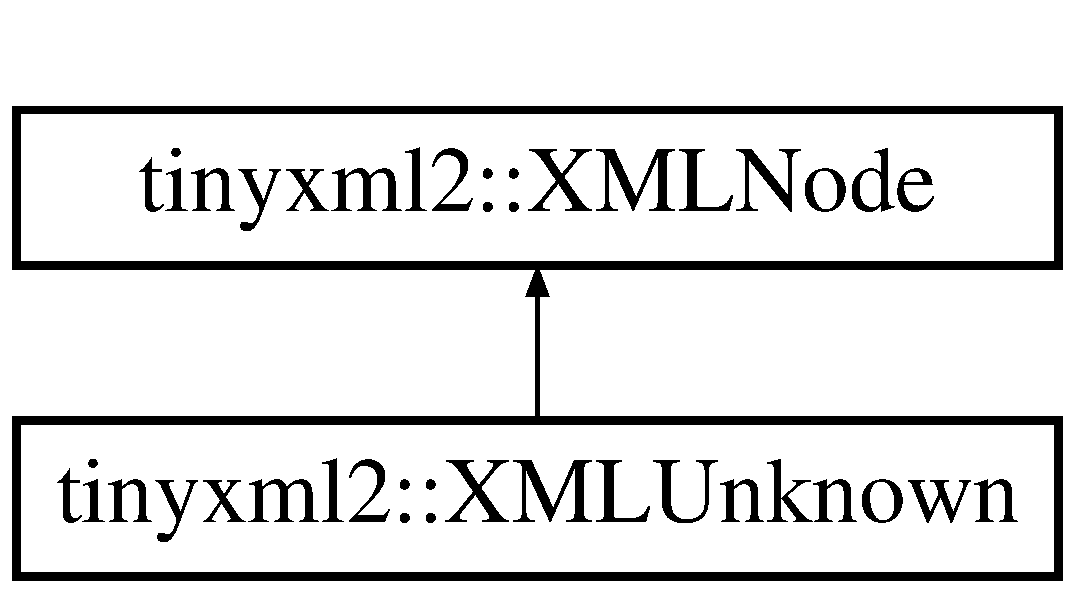
\includegraphics[height=2.000000cm]{classtinyxml2_1_1_x_m_l_unknown}
\end{center}
\end{figure}
\subsection*{Public Member Functions}
\begin{DoxyCompactItemize}
\item 
virtual \hyperlink{classtinyxml2_1_1_x_m_l_unknown}{X\-M\-L\-Unknown} $\ast$ \hyperlink{classtinyxml2_1_1_x_m_l_unknown_af4374856421921cad578c8affae872b6}{To\-Unknown} ()
\begin{DoxyCompactList}\small\item\em Safely cast to an Unknown, or null. \end{DoxyCompactList}\item 
virtual const \hyperlink{classtinyxml2_1_1_x_m_l_unknown}{X\-M\-L\-Unknown} $\ast$ \hyperlink{classtinyxml2_1_1_x_m_l_unknown_a257987e79955399e6e9f119b58d4bb30}{To\-Unknown} () const 
\item 
virtual bool \hyperlink{classtinyxml2_1_1_x_m_l_unknown_a0d341ab804a1438a474810bb5bd29dd5}{Accept} (\hyperlink{classtinyxml2_1_1_x_m_l_visitor}{X\-M\-L\-Visitor} $\ast$visitor) const 
\item 
char $\ast$ \hyperlink{classtinyxml2_1_1_x_m_l_unknown_a0e4f3509dee42a4d45a7f0002be568cc}{Parse\-Deep} (char $\ast$, \hyperlink{classtinyxml2_1_1_str_pair}{Str\-Pair} $\ast$end\-Tag)
\item 
virtual \hyperlink{classtinyxml2_1_1_x_m_l_node}{X\-M\-L\-Node} $\ast$ \hyperlink{classtinyxml2_1_1_x_m_l_unknown_aa09fc7cb0cd64d6bb9c5ae00ffc549ec}{Shallow\-Clone} (\hyperlink{classtinyxml2_1_1_x_m_l_document}{X\-M\-L\-Document} $\ast$document) const 
\item 
virtual bool \hyperlink{classtinyxml2_1_1_x_m_l_unknown_a0169df157bf69a092b404ca49621ff1a}{Shallow\-Equal} (const \hyperlink{classtinyxml2_1_1_x_m_l_node}{X\-M\-L\-Node} $\ast$compare) const 
\end{DoxyCompactItemize}
\subsection*{Protected Member Functions}
\begin{DoxyCompactItemize}
\item 
\hyperlink{classtinyxml2_1_1_x_m_l_unknown_a9391eb679598d50baba424e6f1aa367b}{X\-M\-L\-Unknown} (\hyperlink{classtinyxml2_1_1_x_m_l_document}{X\-M\-L\-Document} $\ast$doc)
\item 
virtual \hyperlink{classtinyxml2_1_1_x_m_l_unknown_a86fcd722ca173a7f385bafafa879f26e}{$\sim$\-X\-M\-L\-Unknown} ()
\item 
\hyperlink{classtinyxml2_1_1_x_m_l_unknown_aab31a93c95a7cedc9597cea7caffa73f}{X\-M\-L\-Unknown} (const \hyperlink{classtinyxml2_1_1_x_m_l_unknown}{X\-M\-L\-Unknown} \&)
\item 
\hyperlink{classtinyxml2_1_1_x_m_l_unknown}{X\-M\-L\-Unknown} \& \hyperlink{classtinyxml2_1_1_x_m_l_unknown_a6137d5611db42c35de3d869f66555e5b}{operator=} (const \hyperlink{classtinyxml2_1_1_x_m_l_unknown}{X\-M\-L\-Unknown} \&)
\end{DoxyCompactItemize}
\subsection*{Friends}
\begin{DoxyCompactItemize}
\item 
class \hyperlink{classtinyxml2_1_1_x_m_l_unknown_a4eee3bda60c60a30e4e8cd4ea91c4c6e}{X\-M\-L\-Document}
\end{DoxyCompactItemize}
\subsection*{Additional Inherited Members}


\subsection{Detailed Description}
Any tag that Tiny\-X\-M\-L-\/2 doesn't recognize is saved as an unknown. It is a tag of text, but should not be modified. It will be written back to the \hyperlink{namespace_x_m_l}{X\-M\-L}, unchanged, when the file is saved.

D\-T\-D tags get thrown into X\-M\-L\-Unknowns. 

Definition at line 948 of file tinyxml2.\-hpp.



\subsection{Constructor \& Destructor Documentation}
\hypertarget{classtinyxml2_1_1_x_m_l_unknown_a9391eb679598d50baba424e6f1aa367b}{\index{tinyxml2\-::\-X\-M\-L\-Unknown@{tinyxml2\-::\-X\-M\-L\-Unknown}!X\-M\-L\-Unknown@{X\-M\-L\-Unknown}}
\index{X\-M\-L\-Unknown@{X\-M\-L\-Unknown}!tinyxml2::XMLUnknown@{tinyxml2\-::\-X\-M\-L\-Unknown}}
\subsubsection[{X\-M\-L\-Unknown}]{\setlength{\rightskip}{0pt plus 5cm}tinyxml2\-::\-X\-M\-L\-Unknown\-::\-X\-M\-L\-Unknown (
\begin{DoxyParamCaption}
\item[{{\bf X\-M\-L\-Document} $\ast$}]{doc}
\end{DoxyParamCaption}
)\hspace{0.3cm}{\ttfamily [protected]}}}\label{classtinyxml2_1_1_x_m_l_unknown_a9391eb679598d50baba424e6f1aa367b}


Definition at line 998 of file tinyxml2.\-cpp.

\hypertarget{classtinyxml2_1_1_x_m_l_unknown_a86fcd722ca173a7f385bafafa879f26e}{\index{tinyxml2\-::\-X\-M\-L\-Unknown@{tinyxml2\-::\-X\-M\-L\-Unknown}!$\sim$\-X\-M\-L\-Unknown@{$\sim$\-X\-M\-L\-Unknown}}
\index{$\sim$\-X\-M\-L\-Unknown@{$\sim$\-X\-M\-L\-Unknown}!tinyxml2::XMLUnknown@{tinyxml2\-::\-X\-M\-L\-Unknown}}
\subsubsection[{$\sim$\-X\-M\-L\-Unknown}]{\setlength{\rightskip}{0pt plus 5cm}tinyxml2\-::\-X\-M\-L\-Unknown\-::$\sim$\-X\-M\-L\-Unknown (
\begin{DoxyParamCaption}
{}
\end{DoxyParamCaption}
)\hspace{0.3cm}{\ttfamily [protected]}, {\ttfamily [virtual]}}}\label{classtinyxml2_1_1_x_m_l_unknown_a86fcd722ca173a7f385bafafa879f26e}


Definition at line 1003 of file tinyxml2.\-cpp.

\hypertarget{classtinyxml2_1_1_x_m_l_unknown_aab31a93c95a7cedc9597cea7caffa73f}{\index{tinyxml2\-::\-X\-M\-L\-Unknown@{tinyxml2\-::\-X\-M\-L\-Unknown}!X\-M\-L\-Unknown@{X\-M\-L\-Unknown}}
\index{X\-M\-L\-Unknown@{X\-M\-L\-Unknown}!tinyxml2::XMLUnknown@{tinyxml2\-::\-X\-M\-L\-Unknown}}
\subsubsection[{X\-M\-L\-Unknown}]{\setlength{\rightskip}{0pt plus 5cm}tinyxml2\-::\-X\-M\-L\-Unknown\-::\-X\-M\-L\-Unknown (
\begin{DoxyParamCaption}
\item[{const {\bf X\-M\-L\-Unknown} \&}]{}
\end{DoxyParamCaption}
)\hspace{0.3cm}{\ttfamily [protected]}}}\label{classtinyxml2_1_1_x_m_l_unknown_aab31a93c95a7cedc9597cea7caffa73f}


\subsection{Member Function Documentation}
\hypertarget{classtinyxml2_1_1_x_m_l_unknown_a0d341ab804a1438a474810bb5bd29dd5}{\index{tinyxml2\-::\-X\-M\-L\-Unknown@{tinyxml2\-::\-X\-M\-L\-Unknown}!Accept@{Accept}}
\index{Accept@{Accept}!tinyxml2::XMLUnknown@{tinyxml2\-::\-X\-M\-L\-Unknown}}
\subsubsection[{Accept}]{\setlength{\rightskip}{0pt plus 5cm}bool tinyxml2\-::\-X\-M\-L\-Unknown\-::\-Accept (
\begin{DoxyParamCaption}
\item[{{\bf X\-M\-L\-Visitor} $\ast$}]{visitor}
\end{DoxyParamCaption}
) const\hspace{0.3cm}{\ttfamily [virtual]}}}\label{classtinyxml2_1_1_x_m_l_unknown_a0d341ab804a1438a474810bb5bd29dd5}
Accept a hierarchical visit of the nodes in the Tiny\-X\-M\-L-\/2 D\-O\-M. Every node in the \hyperlink{namespace_x_m_l}{X\-M\-L} tree will be conditionally visited and the host will be called back via the \hyperlink{classtinyxml2_1_1_x_m_l_visitor}{X\-M\-L\-Visitor} interface.

This is essentially a S\-A\-X interface for Tiny\-X\-M\-L-\/2. (Note however it doesn't re-\/parse the \hyperlink{namespace_x_m_l}{X\-M\-L} for the callbacks, so the performance of Tiny\-X\-M\-L-\/2 is unchanged by using this interface versus any other.)

The interface has been based on ideas from\-:


\begin{DoxyItemize}
\item \href{http://www.saxproject.org/}{\tt http\-://www.\-saxproject.\-org/}
\item \href{http://c2.com/cgi/wiki?HierarchicalVisitorPattern}{\tt http\-://c2.\-com/cgi/wiki?\-Hierarchical\-Visitor\-Pattern}
\end{DoxyItemize}

Which are both good references for \char`\"{}visiting\char`\"{}.

An example of using \hyperlink{classtinyxml2_1_1_x_m_l_unknown_a0d341ab804a1438a474810bb5bd29dd5}{Accept()}\-: \begin{DoxyVerb}XMLPrinter printer;
tinyxmlDoc.Accept( &printer );
const char* xmlcstr = printer.CStr();
\end{DoxyVerb}
 

Implements \hyperlink{classtinyxml2_1_1_x_m_l_node_a81e66df0a44c67a7af17f3b77a152785}{tinyxml2\-::\-X\-M\-L\-Node}.



Definition at line 1037 of file tinyxml2.\-cpp.

\hypertarget{classtinyxml2_1_1_x_m_l_unknown_a6137d5611db42c35de3d869f66555e5b}{\index{tinyxml2\-::\-X\-M\-L\-Unknown@{tinyxml2\-::\-X\-M\-L\-Unknown}!operator=@{operator=}}
\index{operator=@{operator=}!tinyxml2::XMLUnknown@{tinyxml2\-::\-X\-M\-L\-Unknown}}
\subsubsection[{operator=}]{\setlength{\rightskip}{0pt plus 5cm}{\bf X\-M\-L\-Unknown}\& tinyxml2\-::\-X\-M\-L\-Unknown\-::operator= (
\begin{DoxyParamCaption}
\item[{const {\bf X\-M\-L\-Unknown} \&}]{}
\end{DoxyParamCaption}
)\hspace{0.3cm}{\ttfamily [protected]}}}\label{classtinyxml2_1_1_x_m_l_unknown_a6137d5611db42c35de3d869f66555e5b}
\hypertarget{classtinyxml2_1_1_x_m_l_unknown_a0e4f3509dee42a4d45a7f0002be568cc}{\index{tinyxml2\-::\-X\-M\-L\-Unknown@{tinyxml2\-::\-X\-M\-L\-Unknown}!Parse\-Deep@{Parse\-Deep}}
\index{Parse\-Deep@{Parse\-Deep}!tinyxml2::XMLUnknown@{tinyxml2\-::\-X\-M\-L\-Unknown}}
\subsubsection[{Parse\-Deep}]{\setlength{\rightskip}{0pt plus 5cm}char $\ast$ tinyxml2\-::\-X\-M\-L\-Unknown\-::\-Parse\-Deep (
\begin{DoxyParamCaption}
\item[{char $\ast$}]{p, }
\item[{{\bf Str\-Pair} $\ast$}]{end\-Tag}
\end{DoxyParamCaption}
)\hspace{0.3cm}{\ttfamily [virtual]}}}\label{classtinyxml2_1_1_x_m_l_unknown_a0e4f3509dee42a4d45a7f0002be568cc}


Reimplemented from \hyperlink{classtinyxml2_1_1_x_m_l_node_a7610d0f603e8b603d2078521811a23c1}{tinyxml2\-::\-X\-M\-L\-Node}.



Definition at line 1008 of file tinyxml2.\-cpp.

\hypertarget{classtinyxml2_1_1_x_m_l_unknown_aa09fc7cb0cd64d6bb9c5ae00ffc549ec}{\index{tinyxml2\-::\-X\-M\-L\-Unknown@{tinyxml2\-::\-X\-M\-L\-Unknown}!Shallow\-Clone@{Shallow\-Clone}}
\index{Shallow\-Clone@{Shallow\-Clone}!tinyxml2::XMLUnknown@{tinyxml2\-::\-X\-M\-L\-Unknown}}
\subsubsection[{Shallow\-Clone}]{\setlength{\rightskip}{0pt plus 5cm}{\bf X\-M\-L\-Node} $\ast$ tinyxml2\-::\-X\-M\-L\-Unknown\-::\-Shallow\-Clone (
\begin{DoxyParamCaption}
\item[{{\bf X\-M\-L\-Document} $\ast$}]{document}
\end{DoxyParamCaption}
) const\hspace{0.3cm}{\ttfamily [virtual]}}}\label{classtinyxml2_1_1_x_m_l_unknown_aa09fc7cb0cd64d6bb9c5ae00ffc549ec}
Make a copy of this node, but not its children. You may pass in a Document pointer that will be the owner of the new Node. If the 'document' is null, then the node returned will be allocated from the current Document. (this-\/$>$\hyperlink{classtinyxml2_1_1_x_m_l_node_af343d1ef0b45c0020e62d784d7e67a68}{Get\-Document()})

Note\-: if called on a \hyperlink{classtinyxml2_1_1_x_m_l_document}{X\-M\-L\-Document}, this will return null. 

Implements \hyperlink{classtinyxml2_1_1_x_m_l_node_a8402cbd3129d20e9e6024bbcc0531283}{tinyxml2\-::\-X\-M\-L\-Node}.



Definition at line 1021 of file tinyxml2.\-cpp.

\hypertarget{classtinyxml2_1_1_x_m_l_unknown_a0169df157bf69a092b404ca49621ff1a}{\index{tinyxml2\-::\-X\-M\-L\-Unknown@{tinyxml2\-::\-X\-M\-L\-Unknown}!Shallow\-Equal@{Shallow\-Equal}}
\index{Shallow\-Equal@{Shallow\-Equal}!tinyxml2::XMLUnknown@{tinyxml2\-::\-X\-M\-L\-Unknown}}
\subsubsection[{Shallow\-Equal}]{\setlength{\rightskip}{0pt plus 5cm}bool tinyxml2\-::\-X\-M\-L\-Unknown\-::\-Shallow\-Equal (
\begin{DoxyParamCaption}
\item[{const {\bf X\-M\-L\-Node} $\ast$}]{compare}
\end{DoxyParamCaption}
) const\hspace{0.3cm}{\ttfamily [virtual]}}}\label{classtinyxml2_1_1_x_m_l_unknown_a0169df157bf69a092b404ca49621ff1a}
Test if 2 nodes are the same, but don't test children. The 2 nodes do not need to be in the same Document.

Note\-: if called on a \hyperlink{classtinyxml2_1_1_x_m_l_document}{X\-M\-L\-Document}, this will return false. 

Implements \hyperlink{classtinyxml2_1_1_x_m_l_node_a7ce18b751c3ea09eac292dca264f9226}{tinyxml2\-::\-X\-M\-L\-Node}.



Definition at line 1031 of file tinyxml2.\-cpp.

\hypertarget{classtinyxml2_1_1_x_m_l_unknown_af4374856421921cad578c8affae872b6}{\index{tinyxml2\-::\-X\-M\-L\-Unknown@{tinyxml2\-::\-X\-M\-L\-Unknown}!To\-Unknown@{To\-Unknown}}
\index{To\-Unknown@{To\-Unknown}!tinyxml2::XMLUnknown@{tinyxml2\-::\-X\-M\-L\-Unknown}}
\subsubsection[{To\-Unknown}]{\setlength{\rightskip}{0pt plus 5cm}virtual {\bf X\-M\-L\-Unknown}$\ast$ tinyxml2\-::\-X\-M\-L\-Unknown\-::\-To\-Unknown (
\begin{DoxyParamCaption}
{}
\end{DoxyParamCaption}
)\hspace{0.3cm}{\ttfamily [inline]}, {\ttfamily [virtual]}}}\label{classtinyxml2_1_1_x_m_l_unknown_af4374856421921cad578c8affae872b6}


Safely cast to an Unknown, or null. 



Reimplemented from \hyperlink{classtinyxml2_1_1_x_m_l_node_a8675a74aa0ada6eccab0c77ef3e5b9bd}{tinyxml2\-::\-X\-M\-L\-Node}.



Definition at line 952 of file tinyxml2.\-hpp.

\hypertarget{classtinyxml2_1_1_x_m_l_unknown_a257987e79955399e6e9f119b58d4bb30}{\index{tinyxml2\-::\-X\-M\-L\-Unknown@{tinyxml2\-::\-X\-M\-L\-Unknown}!To\-Unknown@{To\-Unknown}}
\index{To\-Unknown@{To\-Unknown}!tinyxml2::XMLUnknown@{tinyxml2\-::\-X\-M\-L\-Unknown}}
\subsubsection[{To\-Unknown}]{\setlength{\rightskip}{0pt plus 5cm}virtual const {\bf X\-M\-L\-Unknown}$\ast$ tinyxml2\-::\-X\-M\-L\-Unknown\-::\-To\-Unknown (
\begin{DoxyParamCaption}
{}
\end{DoxyParamCaption}
) const\hspace{0.3cm}{\ttfamily [inline]}, {\ttfamily [virtual]}}}\label{classtinyxml2_1_1_x_m_l_unknown_a257987e79955399e6e9f119b58d4bb30}


Reimplemented from \hyperlink{classtinyxml2_1_1_x_m_l_node_a71f5ae90296dbe67979f83fe97073efa}{tinyxml2\-::\-X\-M\-L\-Node}.



Definition at line 955 of file tinyxml2.\-hpp.



\subsection{Friends And Related Function Documentation}
\hypertarget{classtinyxml2_1_1_x_m_l_unknown_a4eee3bda60c60a30e4e8cd4ea91c4c6e}{\index{tinyxml2\-::\-X\-M\-L\-Unknown@{tinyxml2\-::\-X\-M\-L\-Unknown}!X\-M\-L\-Document@{X\-M\-L\-Document}}
\index{X\-M\-L\-Document@{X\-M\-L\-Document}!tinyxml2::XMLUnknown@{tinyxml2\-::\-X\-M\-L\-Unknown}}
\subsubsection[{X\-M\-L\-Document}]{\setlength{\rightskip}{0pt plus 5cm}friend class {\bf X\-M\-L\-Document}\hspace{0.3cm}{\ttfamily [friend]}}}\label{classtinyxml2_1_1_x_m_l_unknown_a4eee3bda60c60a30e4e8cd4ea91c4c6e}


Definition at line 950 of file tinyxml2.\-hpp.



The documentation for this class was generated from the following files\-:\begin{DoxyCompactItemize}
\item 
Glide/\hyperlink{tinyxml2_8hpp}{tinyxml2.\-hpp}\item 
Glide/\hyperlink{tinyxml2_8cpp}{tinyxml2.\-cpp}\end{DoxyCompactItemize}

\hypertarget{classtinyxml2_1_1_x_m_l_util}{\section{tinyxml2\-:\-:X\-M\-L\-Util Class Reference}
\label{classtinyxml2_1_1_x_m_l_util}\index{tinyxml2\-::\-X\-M\-L\-Util@{tinyxml2\-::\-X\-M\-L\-Util}}
}


{\ttfamily \#include $<$tinyxml2.\-hpp$>$}

\subsection*{Static Public Member Functions}
\begin{DoxyCompactItemize}
\item 
static const char $\ast$ \hyperlink{classtinyxml2_1_1_x_m_l_util_a9333d20f2a34325b5115ca45849c4b2a}{Skip\-White\-Space} (const char $\ast$p)
\item 
static char $\ast$ \hyperlink{classtinyxml2_1_1_x_m_l_util_aa48025be8843ec5a79b65579d31bd8fc}{Skip\-White\-Space} (char $\ast$p)
\item 
static bool \hyperlink{classtinyxml2_1_1_x_m_l_util_a357ec3af8fc433d19023a815f45e8e33}{Is\-White\-Space} (char p)
\item 
static bool \hyperlink{classtinyxml2_1_1_x_m_l_util_abe106a69ac4d942a4381a4d9dfd0e0bd}{Is\-Name\-Start\-Char} (unsigned char ch)
\item 
static bool \hyperlink{classtinyxml2_1_1_x_m_l_util_a04b17341538fa11752f24b4301d19485}{Is\-Name\-Char} (unsigned char ch)
\item 
static bool \hyperlink{classtinyxml2_1_1_x_m_l_util_acfcd287cacfd2533e1bc9ea4dfb56602}{String\-Equal} (const char $\ast$p, const char $\ast$q, int n\-Char=I\-N\-T\-\_\-\-M\-A\-X)
\item 
static int \hyperlink{classtinyxml2_1_1_x_m_l_util_a24ba87b1d22528167a3d16c4f52096bf}{Is\-U\-T\-F8\-Continuation} (const char p)
\item 
static const char $\ast$ \hyperlink{classtinyxml2_1_1_x_m_l_util_ae9bcb2bc3cd6475fdc644c8c17790555}{Read\-B\-O\-M} (const char $\ast$p, bool $\ast$has\-B\-O\-M)
\item 
static const char $\ast$ \hyperlink{classtinyxml2_1_1_x_m_l_util_a5a96e5144a8d693dc4bcd783d9964648}{Get\-Character\-Ref} (const char $\ast$p, char $\ast$value, int $\ast$length)
\item 
static void \hyperlink{classtinyxml2_1_1_x_m_l_util_a31c00d5c5dfb38382de1dfcaf4be3595}{Convert\-U\-T\-F32\-To\-U\-T\-F8} (unsigned long input, char $\ast$output, int $\ast$length)
\item 
static void \hyperlink{classtinyxml2_1_1_x_m_l_util_a3cd6c703d49b9d51bdf0f4ff6aa021c7}{To\-Str} (int v, char $\ast$buffer, int buffer\-Size)
\item 
static void \hyperlink{classtinyxml2_1_1_x_m_l_util_ac00c2e52c1c36dab3ff41d86a9bf60f9}{To\-Str} (unsigned v, char $\ast$buffer, int buffer\-Size)
\item 
static void \hyperlink{classtinyxml2_1_1_x_m_l_util_adba0718527ae9e80f663a71ea325cb11}{To\-Str} (bool v, char $\ast$buffer, int buffer\-Size)
\item 
static void \hyperlink{classtinyxml2_1_1_x_m_l_util_a8957ad44fee5fa02ba52d73aad4d0a31}{To\-Str} (float v, char $\ast$buffer, int buffer\-Size)
\item 
static void \hyperlink{classtinyxml2_1_1_x_m_l_util_a1cd141e50980fcddd6bf9af5de4b1db7}{To\-Str} (double v, char $\ast$buffer, int buffer\-Size)
\item 
static bool \hyperlink{classtinyxml2_1_1_x_m_l_util_ad4df4023d11ee3fca9689c49b9707323}{To\-Int} (const char $\ast$str, int $\ast$value)
\item 
static bool \hyperlink{classtinyxml2_1_1_x_m_l_util_a210c8637d5eb4ce3d4625294af0efc2f}{To\-Unsigned} (const char $\ast$str, unsigned $\ast$value)
\item 
static bool \hyperlink{classtinyxml2_1_1_x_m_l_util_ae5b03e0a1ca5d42052a7ac540f7aa12a}{To\-Bool} (const char $\ast$str, bool $\ast$value)
\item 
static bool \hyperlink{classtinyxml2_1_1_x_m_l_util_a399e71edb5f29d61ea81d91ee0332bb9}{To\-Float} (const char $\ast$str, float $\ast$value)
\item 
static bool \hyperlink{classtinyxml2_1_1_x_m_l_util_ad8f75ac140fb19c1c6e164a957c4cd53}{To\-Double} (const char $\ast$str, double $\ast$value)
\end{DoxyCompactItemize}


\subsection{Detailed Description}


Definition at line 472 of file tinyxml2.\-hpp.



\subsection{Member Function Documentation}
\hypertarget{classtinyxml2_1_1_x_m_l_util_a31c00d5c5dfb38382de1dfcaf4be3595}{\index{tinyxml2\-::\-X\-M\-L\-Util@{tinyxml2\-::\-X\-M\-L\-Util}!Convert\-U\-T\-F32\-To\-U\-T\-F8@{Convert\-U\-T\-F32\-To\-U\-T\-F8}}
\index{Convert\-U\-T\-F32\-To\-U\-T\-F8@{Convert\-U\-T\-F32\-To\-U\-T\-F8}!tinyxml2::XMLUtil@{tinyxml2\-::\-X\-M\-L\-Util}}
\subsubsection[{Convert\-U\-T\-F32\-To\-U\-T\-F8}]{\setlength{\rightskip}{0pt plus 5cm}void tinyxml2\-::\-X\-M\-L\-Util\-::\-Convert\-U\-T\-F32\-To\-U\-T\-F8 (
\begin{DoxyParamCaption}
\item[{unsigned long}]{input, }
\item[{char $\ast$}]{output, }
\item[{int $\ast$}]{length}
\end{DoxyParamCaption}
)\hspace{0.3cm}{\ttfamily [static]}}}\label{classtinyxml2_1_1_x_m_l_util_a31c00d5c5dfb38382de1dfcaf4be3595}


Definition at line 282 of file tinyxml2.\-cpp.

\hypertarget{classtinyxml2_1_1_x_m_l_util_a5a96e5144a8d693dc4bcd783d9964648}{\index{tinyxml2\-::\-X\-M\-L\-Util@{tinyxml2\-::\-X\-M\-L\-Util}!Get\-Character\-Ref@{Get\-Character\-Ref}}
\index{Get\-Character\-Ref@{Get\-Character\-Ref}!tinyxml2::XMLUtil@{tinyxml2\-::\-X\-M\-L\-Util}}
\subsubsection[{Get\-Character\-Ref}]{\setlength{\rightskip}{0pt plus 5cm}const char $\ast$ tinyxml2\-::\-X\-M\-L\-Util\-::\-Get\-Character\-Ref (
\begin{DoxyParamCaption}
\item[{const char $\ast$}]{p, }
\item[{char $\ast$}]{value, }
\item[{int $\ast$}]{length}
\end{DoxyParamCaption}
)\hspace{0.3cm}{\ttfamily [static]}}}\label{classtinyxml2_1_1_x_m_l_util_a5a96e5144a8d693dc4bcd783d9964648}


Definition at line 330 of file tinyxml2.\-cpp.

\hypertarget{classtinyxml2_1_1_x_m_l_util_a04b17341538fa11752f24b4301d19485}{\index{tinyxml2\-::\-X\-M\-L\-Util@{tinyxml2\-::\-X\-M\-L\-Util}!Is\-Name\-Char@{Is\-Name\-Char}}
\index{Is\-Name\-Char@{Is\-Name\-Char}!tinyxml2::XMLUtil@{tinyxml2\-::\-X\-M\-L\-Util}}
\subsubsection[{Is\-Name\-Char}]{\setlength{\rightskip}{0pt plus 5cm}static bool tinyxml2\-::\-X\-M\-L\-Util\-::\-Is\-Name\-Char (
\begin{DoxyParamCaption}
\item[{unsigned char}]{ch}
\end{DoxyParamCaption}
)\hspace{0.3cm}{\ttfamily [inline]}, {\ttfamily [static]}}}\label{classtinyxml2_1_1_x_m_l_util_a04b17341538fa11752f24b4301d19485}


Definition at line 499 of file tinyxml2.\-hpp.

\hypertarget{classtinyxml2_1_1_x_m_l_util_abe106a69ac4d942a4381a4d9dfd0e0bd}{\index{tinyxml2\-::\-X\-M\-L\-Util@{tinyxml2\-::\-X\-M\-L\-Util}!Is\-Name\-Start\-Char@{Is\-Name\-Start\-Char}}
\index{Is\-Name\-Start\-Char@{Is\-Name\-Start\-Char}!tinyxml2::XMLUtil@{tinyxml2\-::\-X\-M\-L\-Util}}
\subsubsection[{Is\-Name\-Start\-Char}]{\setlength{\rightskip}{0pt plus 5cm}static bool tinyxml2\-::\-X\-M\-L\-Util\-::\-Is\-Name\-Start\-Char (
\begin{DoxyParamCaption}
\item[{unsigned char}]{ch}
\end{DoxyParamCaption}
)\hspace{0.3cm}{\ttfamily [inline]}, {\ttfamily [static]}}}\label{classtinyxml2_1_1_x_m_l_util_abe106a69ac4d942a4381a4d9dfd0e0bd}


Definition at line 493 of file tinyxml2.\-hpp.

\hypertarget{classtinyxml2_1_1_x_m_l_util_a24ba87b1d22528167a3d16c4f52096bf}{\index{tinyxml2\-::\-X\-M\-L\-Util@{tinyxml2\-::\-X\-M\-L\-Util}!Is\-U\-T\-F8\-Continuation@{Is\-U\-T\-F8\-Continuation}}
\index{Is\-U\-T\-F8\-Continuation@{Is\-U\-T\-F8\-Continuation}!tinyxml2::XMLUtil@{tinyxml2\-::\-X\-M\-L\-Util}}
\subsubsection[{Is\-U\-T\-F8\-Continuation}]{\setlength{\rightskip}{0pt plus 5cm}static int tinyxml2\-::\-X\-M\-L\-Util\-::\-Is\-U\-T\-F8\-Continuation (
\begin{DoxyParamCaption}
\item[{const char}]{p}
\end{DoxyParamCaption}
)\hspace{0.3cm}{\ttfamily [inline]}, {\ttfamily [static]}}}\label{classtinyxml2_1_1_x_m_l_util_a24ba87b1d22528167a3d16c4f52096bf}


Definition at line 522 of file tinyxml2.\-hpp.

\hypertarget{classtinyxml2_1_1_x_m_l_util_a357ec3af8fc433d19023a815f45e8e33}{\index{tinyxml2\-::\-X\-M\-L\-Util@{tinyxml2\-::\-X\-M\-L\-Util}!Is\-White\-Space@{Is\-White\-Space}}
\index{Is\-White\-Space@{Is\-White\-Space}!tinyxml2::XMLUtil@{tinyxml2\-::\-X\-M\-L\-Util}}
\subsubsection[{Is\-White\-Space}]{\setlength{\rightskip}{0pt plus 5cm}static bool tinyxml2\-::\-X\-M\-L\-Util\-::\-Is\-White\-Space (
\begin{DoxyParamCaption}
\item[{char}]{p}
\end{DoxyParamCaption}
)\hspace{0.3cm}{\ttfamily [inline]}, {\ttfamily [static]}}}\label{classtinyxml2_1_1_x_m_l_util_a357ec3af8fc433d19023a815f45e8e33}


Definition at line 489 of file tinyxml2.\-hpp.

\hypertarget{classtinyxml2_1_1_x_m_l_util_ae9bcb2bc3cd6475fdc644c8c17790555}{\index{tinyxml2\-::\-X\-M\-L\-Util@{tinyxml2\-::\-X\-M\-L\-Util}!Read\-B\-O\-M@{Read\-B\-O\-M}}
\index{Read\-B\-O\-M@{Read\-B\-O\-M}!tinyxml2::XMLUtil@{tinyxml2\-::\-X\-M\-L\-Util}}
\subsubsection[{Read\-B\-O\-M}]{\setlength{\rightskip}{0pt plus 5cm}const char $\ast$ tinyxml2\-::\-X\-M\-L\-Util\-::\-Read\-B\-O\-M (
\begin{DoxyParamCaption}
\item[{const char $\ast$}]{p, }
\item[{bool $\ast$}]{has\-B\-O\-M}
\end{DoxyParamCaption}
)\hspace{0.3cm}{\ttfamily [static]}}}\label{classtinyxml2_1_1_x_m_l_util_ae9bcb2bc3cd6475fdc644c8c17790555}


Definition at line 267 of file tinyxml2.\-cpp.

\hypertarget{classtinyxml2_1_1_x_m_l_util_a9333d20f2a34325b5115ca45849c4b2a}{\index{tinyxml2\-::\-X\-M\-L\-Util@{tinyxml2\-::\-X\-M\-L\-Util}!Skip\-White\-Space@{Skip\-White\-Space}}
\index{Skip\-White\-Space@{Skip\-White\-Space}!tinyxml2::XMLUtil@{tinyxml2\-::\-X\-M\-L\-Util}}
\subsubsection[{Skip\-White\-Space}]{\setlength{\rightskip}{0pt plus 5cm}static const char$\ast$ tinyxml2\-::\-X\-M\-L\-Util\-::\-Skip\-White\-Space (
\begin{DoxyParamCaption}
\item[{const char $\ast$}]{p}
\end{DoxyParamCaption}
)\hspace{0.3cm}{\ttfamily [inline]}, {\ttfamily [static]}}}\label{classtinyxml2_1_1_x_m_l_util_a9333d20f2a34325b5115ca45849c4b2a}


Definition at line 477 of file tinyxml2.\-hpp.

\hypertarget{classtinyxml2_1_1_x_m_l_util_aa48025be8843ec5a79b65579d31bd8fc}{\index{tinyxml2\-::\-X\-M\-L\-Util@{tinyxml2\-::\-X\-M\-L\-Util}!Skip\-White\-Space@{Skip\-White\-Space}}
\index{Skip\-White\-Space@{Skip\-White\-Space}!tinyxml2::XMLUtil@{tinyxml2\-::\-X\-M\-L\-Util}}
\subsubsection[{Skip\-White\-Space}]{\setlength{\rightskip}{0pt plus 5cm}static char$\ast$ tinyxml2\-::\-X\-M\-L\-Util\-::\-Skip\-White\-Space (
\begin{DoxyParamCaption}
\item[{char $\ast$}]{p}
\end{DoxyParamCaption}
)\hspace{0.3cm}{\ttfamily [inline]}, {\ttfamily [static]}}}\label{classtinyxml2_1_1_x_m_l_util_aa48025be8843ec5a79b65579d31bd8fc}


Definition at line 483 of file tinyxml2.\-hpp.

\hypertarget{classtinyxml2_1_1_x_m_l_util_acfcd287cacfd2533e1bc9ea4dfb56602}{\index{tinyxml2\-::\-X\-M\-L\-Util@{tinyxml2\-::\-X\-M\-L\-Util}!String\-Equal@{String\-Equal}}
\index{String\-Equal@{String\-Equal}!tinyxml2::XMLUtil@{tinyxml2\-::\-X\-M\-L\-Util}}
\subsubsection[{String\-Equal}]{\setlength{\rightskip}{0pt plus 5cm}static bool tinyxml2\-::\-X\-M\-L\-Util\-::\-String\-Equal (
\begin{DoxyParamCaption}
\item[{const char $\ast$}]{p, }
\item[{const char $\ast$}]{q, }
\item[{int}]{n\-Char = {\ttfamily INT\-\_\-MAX}}
\end{DoxyParamCaption}
)\hspace{0.3cm}{\ttfamily [inline]}, {\ttfamily [static]}}}\label{classtinyxml2_1_1_x_m_l_util_acfcd287cacfd2533e1bc9ea4dfb56602}


Definition at line 506 of file tinyxml2.\-hpp.

\hypertarget{classtinyxml2_1_1_x_m_l_util_ae5b03e0a1ca5d42052a7ac540f7aa12a}{\index{tinyxml2\-::\-X\-M\-L\-Util@{tinyxml2\-::\-X\-M\-L\-Util}!To\-Bool@{To\-Bool}}
\index{To\-Bool@{To\-Bool}!tinyxml2::XMLUtil@{tinyxml2\-::\-X\-M\-L\-Util}}
\subsubsection[{To\-Bool}]{\setlength{\rightskip}{0pt plus 5cm}bool tinyxml2\-::\-X\-M\-L\-Util\-::\-To\-Bool (
\begin{DoxyParamCaption}
\item[{const char $\ast$}]{str, }
\item[{bool $\ast$}]{value}
\end{DoxyParamCaption}
)\hspace{0.3cm}{\ttfamily [static]}}}\label{classtinyxml2_1_1_x_m_l_util_ae5b03e0a1ca5d42052a7ac540f7aa12a}


Definition at line 454 of file tinyxml2.\-cpp.

\hypertarget{classtinyxml2_1_1_x_m_l_util_ad8f75ac140fb19c1c6e164a957c4cd53}{\index{tinyxml2\-::\-X\-M\-L\-Util@{tinyxml2\-::\-X\-M\-L\-Util}!To\-Double@{To\-Double}}
\index{To\-Double@{To\-Double}!tinyxml2::XMLUtil@{tinyxml2\-::\-X\-M\-L\-Util}}
\subsubsection[{To\-Double}]{\setlength{\rightskip}{0pt plus 5cm}bool tinyxml2\-::\-X\-M\-L\-Util\-::\-To\-Double (
\begin{DoxyParamCaption}
\item[{const char $\ast$}]{str, }
\item[{double $\ast$}]{value}
\end{DoxyParamCaption}
)\hspace{0.3cm}{\ttfamily [static]}}}\label{classtinyxml2_1_1_x_m_l_util_ad8f75ac140fb19c1c6e164a957c4cd53}


Definition at line 481 of file tinyxml2.\-cpp.

\hypertarget{classtinyxml2_1_1_x_m_l_util_a399e71edb5f29d61ea81d91ee0332bb9}{\index{tinyxml2\-::\-X\-M\-L\-Util@{tinyxml2\-::\-X\-M\-L\-Util}!To\-Float@{To\-Float}}
\index{To\-Float@{To\-Float}!tinyxml2::XMLUtil@{tinyxml2\-::\-X\-M\-L\-Util}}
\subsubsection[{To\-Float}]{\setlength{\rightskip}{0pt plus 5cm}bool tinyxml2\-::\-X\-M\-L\-Util\-::\-To\-Float (
\begin{DoxyParamCaption}
\item[{const char $\ast$}]{str, }
\item[{float $\ast$}]{value}
\end{DoxyParamCaption}
)\hspace{0.3cm}{\ttfamily [static]}}}\label{classtinyxml2_1_1_x_m_l_util_a399e71edb5f29d61ea81d91ee0332bb9}


Definition at line 473 of file tinyxml2.\-cpp.

\hypertarget{classtinyxml2_1_1_x_m_l_util_ad4df4023d11ee3fca9689c49b9707323}{\index{tinyxml2\-::\-X\-M\-L\-Util@{tinyxml2\-::\-X\-M\-L\-Util}!To\-Int@{To\-Int}}
\index{To\-Int@{To\-Int}!tinyxml2::XMLUtil@{tinyxml2\-::\-X\-M\-L\-Util}}
\subsubsection[{To\-Int}]{\setlength{\rightskip}{0pt plus 5cm}bool tinyxml2\-::\-X\-M\-L\-Util\-::\-To\-Int (
\begin{DoxyParamCaption}
\item[{const char $\ast$}]{str, }
\item[{int $\ast$}]{value}
\end{DoxyParamCaption}
)\hspace{0.3cm}{\ttfamily [static]}}}\label{classtinyxml2_1_1_x_m_l_util_ad4df4023d11ee3fca9689c49b9707323}


Definition at line 438 of file tinyxml2.\-cpp.

\hypertarget{classtinyxml2_1_1_x_m_l_util_a3cd6c703d49b9d51bdf0f4ff6aa021c7}{\index{tinyxml2\-::\-X\-M\-L\-Util@{tinyxml2\-::\-X\-M\-L\-Util}!To\-Str@{To\-Str}}
\index{To\-Str@{To\-Str}!tinyxml2::XMLUtil@{tinyxml2\-::\-X\-M\-L\-Util}}
\subsubsection[{To\-Str}]{\setlength{\rightskip}{0pt plus 5cm}void tinyxml2\-::\-X\-M\-L\-Util\-::\-To\-Str (
\begin{DoxyParamCaption}
\item[{int}]{v, }
\item[{char $\ast$}]{buffer, }
\item[{int}]{buffer\-Size}
\end{DoxyParamCaption}
)\hspace{0.3cm}{\ttfamily [static]}}}\label{classtinyxml2_1_1_x_m_l_util_a3cd6c703d49b9d51bdf0f4ff6aa021c7}


Definition at line 408 of file tinyxml2.\-cpp.

\hypertarget{classtinyxml2_1_1_x_m_l_util_ac00c2e52c1c36dab3ff41d86a9bf60f9}{\index{tinyxml2\-::\-X\-M\-L\-Util@{tinyxml2\-::\-X\-M\-L\-Util}!To\-Str@{To\-Str}}
\index{To\-Str@{To\-Str}!tinyxml2::XMLUtil@{tinyxml2\-::\-X\-M\-L\-Util}}
\subsubsection[{To\-Str}]{\setlength{\rightskip}{0pt plus 5cm}void tinyxml2\-::\-X\-M\-L\-Util\-::\-To\-Str (
\begin{DoxyParamCaption}
\item[{unsigned}]{v, }
\item[{char $\ast$}]{buffer, }
\item[{int}]{buffer\-Size}
\end{DoxyParamCaption}
)\hspace{0.3cm}{\ttfamily [static]}}}\label{classtinyxml2_1_1_x_m_l_util_ac00c2e52c1c36dab3ff41d86a9bf60f9}


Definition at line 414 of file tinyxml2.\-cpp.

\hypertarget{classtinyxml2_1_1_x_m_l_util_adba0718527ae9e80f663a71ea325cb11}{\index{tinyxml2\-::\-X\-M\-L\-Util@{tinyxml2\-::\-X\-M\-L\-Util}!To\-Str@{To\-Str}}
\index{To\-Str@{To\-Str}!tinyxml2::XMLUtil@{tinyxml2\-::\-X\-M\-L\-Util}}
\subsubsection[{To\-Str}]{\setlength{\rightskip}{0pt plus 5cm}void tinyxml2\-::\-X\-M\-L\-Util\-::\-To\-Str (
\begin{DoxyParamCaption}
\item[{bool}]{v, }
\item[{char $\ast$}]{buffer, }
\item[{int}]{buffer\-Size}
\end{DoxyParamCaption}
)\hspace{0.3cm}{\ttfamily [static]}}}\label{classtinyxml2_1_1_x_m_l_util_adba0718527ae9e80f663a71ea325cb11}


Definition at line 420 of file tinyxml2.\-cpp.

\hypertarget{classtinyxml2_1_1_x_m_l_util_a8957ad44fee5fa02ba52d73aad4d0a31}{\index{tinyxml2\-::\-X\-M\-L\-Util@{tinyxml2\-::\-X\-M\-L\-Util}!To\-Str@{To\-Str}}
\index{To\-Str@{To\-Str}!tinyxml2::XMLUtil@{tinyxml2\-::\-X\-M\-L\-Util}}
\subsubsection[{To\-Str}]{\setlength{\rightskip}{0pt plus 5cm}void tinyxml2\-::\-X\-M\-L\-Util\-::\-To\-Str (
\begin{DoxyParamCaption}
\item[{float}]{v, }
\item[{char $\ast$}]{buffer, }
\item[{int}]{buffer\-Size}
\end{DoxyParamCaption}
)\hspace{0.3cm}{\ttfamily [static]}}}\label{classtinyxml2_1_1_x_m_l_util_a8957ad44fee5fa02ba52d73aad4d0a31}


Definition at line 426 of file tinyxml2.\-cpp.

\hypertarget{classtinyxml2_1_1_x_m_l_util_a1cd141e50980fcddd6bf9af5de4b1db7}{\index{tinyxml2\-::\-X\-M\-L\-Util@{tinyxml2\-::\-X\-M\-L\-Util}!To\-Str@{To\-Str}}
\index{To\-Str@{To\-Str}!tinyxml2::XMLUtil@{tinyxml2\-::\-X\-M\-L\-Util}}
\subsubsection[{To\-Str}]{\setlength{\rightskip}{0pt plus 5cm}void tinyxml2\-::\-X\-M\-L\-Util\-::\-To\-Str (
\begin{DoxyParamCaption}
\item[{double}]{v, }
\item[{char $\ast$}]{buffer, }
\item[{int}]{buffer\-Size}
\end{DoxyParamCaption}
)\hspace{0.3cm}{\ttfamily [static]}}}\label{classtinyxml2_1_1_x_m_l_util_a1cd141e50980fcddd6bf9af5de4b1db7}


Definition at line 432 of file tinyxml2.\-cpp.

\hypertarget{classtinyxml2_1_1_x_m_l_util_a210c8637d5eb4ce3d4625294af0efc2f}{\index{tinyxml2\-::\-X\-M\-L\-Util@{tinyxml2\-::\-X\-M\-L\-Util}!To\-Unsigned@{To\-Unsigned}}
\index{To\-Unsigned@{To\-Unsigned}!tinyxml2::XMLUtil@{tinyxml2\-::\-X\-M\-L\-Util}}
\subsubsection[{To\-Unsigned}]{\setlength{\rightskip}{0pt plus 5cm}bool tinyxml2\-::\-X\-M\-L\-Util\-::\-To\-Unsigned (
\begin{DoxyParamCaption}
\item[{const char $\ast$}]{str, }
\item[{unsigned $\ast$}]{value}
\end{DoxyParamCaption}
)\hspace{0.3cm}{\ttfamily [static]}}}\label{classtinyxml2_1_1_x_m_l_util_a210c8637d5eb4ce3d4625294af0efc2f}


Definition at line 446 of file tinyxml2.\-cpp.



The documentation for this class was generated from the following files\-:\begin{DoxyCompactItemize}
\item 
Glide/\hyperlink{tinyxml2_8hpp}{tinyxml2.\-hpp}\item 
Glide/\hyperlink{tinyxml2_8cpp}{tinyxml2.\-cpp}\end{DoxyCompactItemize}

\hypertarget{classtinyxml2_1_1_x_m_l_visitor}{\section{tinyxml2\-:\-:X\-M\-L\-Visitor Class Reference}
\label{classtinyxml2_1_1_x_m_l_visitor}\index{tinyxml2\-::\-X\-M\-L\-Visitor@{tinyxml2\-::\-X\-M\-L\-Visitor}}
}


{\ttfamily \#include $<$tinyxml2.\-hpp$>$}

Inheritance diagram for tinyxml2\-:\-:X\-M\-L\-Visitor\-:\begin{figure}[H]
\begin{center}
\leavevmode
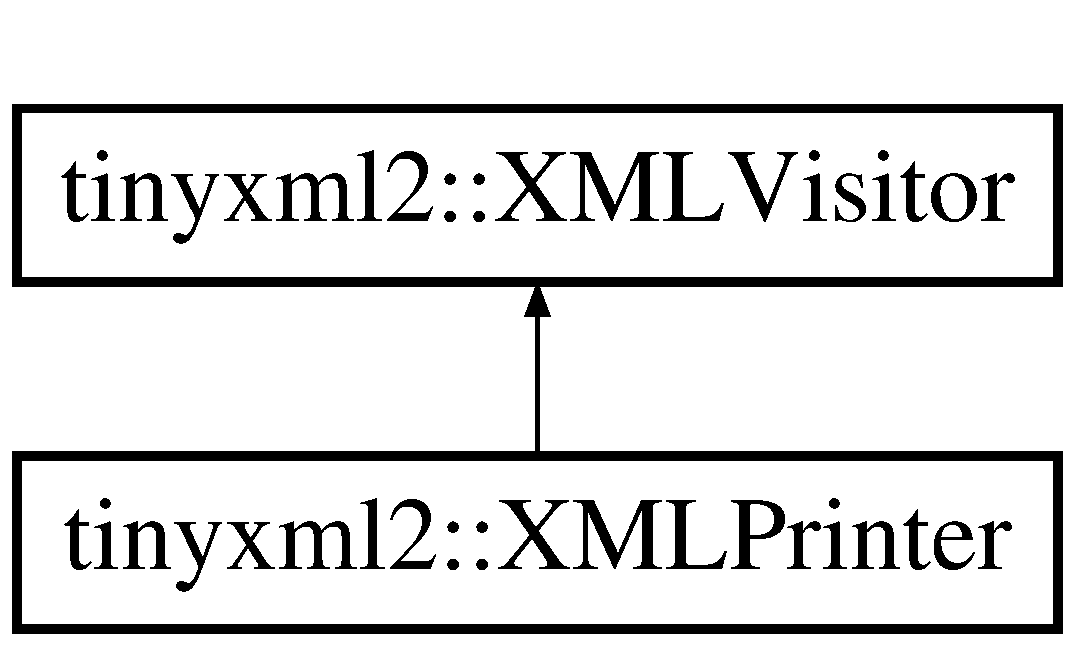
\includegraphics[height=2.000000cm]{classtinyxml2_1_1_x_m_l_visitor}
\end{center}
\end{figure}
\subsection*{Public Member Functions}
\begin{DoxyCompactItemize}
\item 
virtual \hyperlink{classtinyxml2_1_1_x_m_l_visitor_a494e72033d646c47d9c65c502ec62364}{$\sim$\-X\-M\-L\-Visitor} ()
\item 
virtual bool \hyperlink{classtinyxml2_1_1_x_m_l_visitor_acb3c22fc5f60eb9db98f533f2761f67d}{Visit\-Enter} (const \hyperlink{classtinyxml2_1_1_x_m_l_document}{X\-M\-L\-Document} \&)
\begin{DoxyCompactList}\small\item\em Visit a document. \end{DoxyCompactList}\item 
virtual bool \hyperlink{classtinyxml2_1_1_x_m_l_visitor_a170e9989cd046ba904f302d087e07086}{Visit\-Exit} (const \hyperlink{classtinyxml2_1_1_x_m_l_document}{X\-M\-L\-Document} \&)
\begin{DoxyCompactList}\small\item\em Visit a document. \end{DoxyCompactList}\item 
virtual bool \hyperlink{classtinyxml2_1_1_x_m_l_visitor_af97980a17dd4e37448b181f5ddfa92b5}{Visit\-Enter} (const \hyperlink{classtinyxml2_1_1_x_m_l_element}{X\-M\-L\-Element} \&, const \hyperlink{classtinyxml2_1_1_x_m_l_attribute}{X\-M\-L\-Attribute} $\ast$)
\begin{DoxyCompactList}\small\item\em Visit an element. \end{DoxyCompactList}\item 
virtual bool \hyperlink{classtinyxml2_1_1_x_m_l_visitor_a772f10ddc83f881956d32628faa16eb6}{Visit\-Exit} (const \hyperlink{classtinyxml2_1_1_x_m_l_element}{X\-M\-L\-Element} \&)
\begin{DoxyCompactList}\small\item\em Visit an element. \end{DoxyCompactList}\item 
virtual bool \hyperlink{classtinyxml2_1_1_x_m_l_visitor_adc75bd459fc7ba8223b50f0616767f9a}{Visit} (const \hyperlink{classtinyxml2_1_1_x_m_l_declaration}{X\-M\-L\-Declaration} \&)
\begin{DoxyCompactList}\small\item\em Visit a declaration. \end{DoxyCompactList}\item 
virtual bool \hyperlink{classtinyxml2_1_1_x_m_l_visitor_af30233565856480ea48b6fa0d6dec65b}{Visit} (const \hyperlink{classtinyxml2_1_1_x_m_l_text}{X\-M\-L\-Text} \&)
\begin{DoxyCompactList}\small\item\em Visit a text node. \end{DoxyCompactList}\item 
virtual bool \hyperlink{classtinyxml2_1_1_x_m_l_visitor_acc8147fb5a85f6c65721654e427752d7}{Visit} (const \hyperlink{classtinyxml2_1_1_x_m_l_comment}{X\-M\-L\-Comment} \&)
\begin{DoxyCompactList}\small\item\em Visit a comment node. \end{DoxyCompactList}\item 
virtual bool \hyperlink{classtinyxml2_1_1_x_m_l_visitor_a14e4748387c34bf53d24e8119bb1f292}{Visit} (const \hyperlink{classtinyxml2_1_1_x_m_l_unknown}{X\-M\-L\-Unknown} \&)
\begin{DoxyCompactList}\small\item\em Visit an unknown node. \end{DoxyCompactList}\end{DoxyCompactItemize}


\subsection{Detailed Description}
Implements the interface to the \char`\"{}\-Visitor pattern\char`\"{} (see the Accept() method.) If you call the Accept() method, it requires being passed a \hyperlink{classtinyxml2_1_1_x_m_l_visitor}{X\-M\-L\-Visitor} class to handle callbacks. For nodes that contain other nodes (Document, Element) you will get called with a Visit\-Enter/\-Visit\-Exit pair. Nodes that are always leafs are simply called with \hyperlink{classtinyxml2_1_1_x_m_l_visitor_adc75bd459fc7ba8223b50f0616767f9a}{Visit()}.

If you return 'true' from a Visit method, recursive parsing will continue. If you return false, {\bfseries no children of this node or its siblings} will be visited.

All flavors of Visit methods have a default implementation that returns 'true' (continue visiting). You need to only override methods that are interesting to you.

Generally Accept() is called on the \hyperlink{classtinyxml2_1_1_x_m_l_document}{X\-M\-L\-Document}, although all nodes support visiting.

You should never change the document from a callback.

\begin{DoxySeeAlso}{See Also}
\hyperlink{classtinyxml2_1_1_x_m_l_node_a81e66df0a44c67a7af17f3b77a152785}{X\-M\-L\-Node\-::\-Accept()} 
\end{DoxySeeAlso}


Definition at line 427 of file tinyxml2.\-hpp.



\subsection{Constructor \& Destructor Documentation}
\hypertarget{classtinyxml2_1_1_x_m_l_visitor_a494e72033d646c47d9c65c502ec62364}{\index{tinyxml2\-::\-X\-M\-L\-Visitor@{tinyxml2\-::\-X\-M\-L\-Visitor}!$\sim$\-X\-M\-L\-Visitor@{$\sim$\-X\-M\-L\-Visitor}}
\index{$\sim$\-X\-M\-L\-Visitor@{$\sim$\-X\-M\-L\-Visitor}!tinyxml2::XMLVisitor@{tinyxml2\-::\-X\-M\-L\-Visitor}}
\subsubsection[{$\sim$\-X\-M\-L\-Visitor}]{\setlength{\rightskip}{0pt plus 5cm}virtual tinyxml2\-::\-X\-M\-L\-Visitor\-::$\sim$\-X\-M\-L\-Visitor (
\begin{DoxyParamCaption}
{}
\end{DoxyParamCaption}
)\hspace{0.3cm}{\ttfamily [inline]}, {\ttfamily [virtual]}}}\label{classtinyxml2_1_1_x_m_l_visitor_a494e72033d646c47d9c65c502ec62364}


Definition at line 430 of file tinyxml2.\-hpp.



\subsection{Member Function Documentation}
\hypertarget{classtinyxml2_1_1_x_m_l_visitor_adc75bd459fc7ba8223b50f0616767f9a}{\index{tinyxml2\-::\-X\-M\-L\-Visitor@{tinyxml2\-::\-X\-M\-L\-Visitor}!Visit@{Visit}}
\index{Visit@{Visit}!tinyxml2::XMLVisitor@{tinyxml2\-::\-X\-M\-L\-Visitor}}
\subsubsection[{Visit}]{\setlength{\rightskip}{0pt plus 5cm}virtual bool tinyxml2\-::\-X\-M\-L\-Visitor\-::\-Visit (
\begin{DoxyParamCaption}
\item[{const {\bf X\-M\-L\-Declaration} \&}]{}
\end{DoxyParamCaption}
)\hspace{0.3cm}{\ttfamily [inline]}, {\ttfamily [virtual]}}}\label{classtinyxml2_1_1_x_m_l_visitor_adc75bd459fc7ba8223b50f0616767f9a}


Visit a declaration. 



Reimplemented in \hyperlink{classtinyxml2_1_1_x_m_l_printer_acfc625b2549304b9c7eb85ebd5c5eb39}{tinyxml2\-::\-X\-M\-L\-Printer}.



Definition at line 451 of file tinyxml2.\-hpp.

\hypertarget{classtinyxml2_1_1_x_m_l_visitor_af30233565856480ea48b6fa0d6dec65b}{\index{tinyxml2\-::\-X\-M\-L\-Visitor@{tinyxml2\-::\-X\-M\-L\-Visitor}!Visit@{Visit}}
\index{Visit@{Visit}!tinyxml2::XMLVisitor@{tinyxml2\-::\-X\-M\-L\-Visitor}}
\subsubsection[{Visit}]{\setlength{\rightskip}{0pt plus 5cm}virtual bool tinyxml2\-::\-X\-M\-L\-Visitor\-::\-Visit (
\begin{DoxyParamCaption}
\item[{const {\bf X\-M\-L\-Text} \&}]{}
\end{DoxyParamCaption}
)\hspace{0.3cm}{\ttfamily [inline]}, {\ttfamily [virtual]}}}\label{classtinyxml2_1_1_x_m_l_visitor_af30233565856480ea48b6fa0d6dec65b}


Visit a text node. 



Reimplemented in \hyperlink{classtinyxml2_1_1_x_m_l_printer_adc0e42b4f6fcb90a95630c79575d030b}{tinyxml2\-::\-X\-M\-L\-Printer}.



Definition at line 455 of file tinyxml2.\-hpp.

\hypertarget{classtinyxml2_1_1_x_m_l_visitor_acc8147fb5a85f6c65721654e427752d7}{\index{tinyxml2\-::\-X\-M\-L\-Visitor@{tinyxml2\-::\-X\-M\-L\-Visitor}!Visit@{Visit}}
\index{Visit@{Visit}!tinyxml2::XMLVisitor@{tinyxml2\-::\-X\-M\-L\-Visitor}}
\subsubsection[{Visit}]{\setlength{\rightskip}{0pt plus 5cm}virtual bool tinyxml2\-::\-X\-M\-L\-Visitor\-::\-Visit (
\begin{DoxyParamCaption}
\item[{const {\bf X\-M\-L\-Comment} \&}]{}
\end{DoxyParamCaption}
)\hspace{0.3cm}{\ttfamily [inline]}, {\ttfamily [virtual]}}}\label{classtinyxml2_1_1_x_m_l_visitor_acc8147fb5a85f6c65721654e427752d7}


Visit a comment node. 



Reimplemented in \hyperlink{classtinyxml2_1_1_x_m_l_printer_aa294c5c01af0ebb9114902456e4cb53c}{tinyxml2\-::\-X\-M\-L\-Printer}.



Definition at line 459 of file tinyxml2.\-hpp.

\hypertarget{classtinyxml2_1_1_x_m_l_visitor_a14e4748387c34bf53d24e8119bb1f292}{\index{tinyxml2\-::\-X\-M\-L\-Visitor@{tinyxml2\-::\-X\-M\-L\-Visitor}!Visit@{Visit}}
\index{Visit@{Visit}!tinyxml2::XMLVisitor@{tinyxml2\-::\-X\-M\-L\-Visitor}}
\subsubsection[{Visit}]{\setlength{\rightskip}{0pt plus 5cm}virtual bool tinyxml2\-::\-X\-M\-L\-Visitor\-::\-Visit (
\begin{DoxyParamCaption}
\item[{const {\bf X\-M\-L\-Unknown} \&}]{}
\end{DoxyParamCaption}
)\hspace{0.3cm}{\ttfamily [inline]}, {\ttfamily [virtual]}}}\label{classtinyxml2_1_1_x_m_l_visitor_a14e4748387c34bf53d24e8119bb1f292}


Visit an unknown node. 



Reimplemented in \hyperlink{classtinyxml2_1_1_x_m_l_printer_ab8af5455bbf9e4be2663e6642fcd7e32}{tinyxml2\-::\-X\-M\-L\-Printer}.



Definition at line 463 of file tinyxml2.\-hpp.

\hypertarget{classtinyxml2_1_1_x_m_l_visitor_acb3c22fc5f60eb9db98f533f2761f67d}{\index{tinyxml2\-::\-X\-M\-L\-Visitor@{tinyxml2\-::\-X\-M\-L\-Visitor}!Visit\-Enter@{Visit\-Enter}}
\index{Visit\-Enter@{Visit\-Enter}!tinyxml2::XMLVisitor@{tinyxml2\-::\-X\-M\-L\-Visitor}}
\subsubsection[{Visit\-Enter}]{\setlength{\rightskip}{0pt plus 5cm}virtual bool tinyxml2\-::\-X\-M\-L\-Visitor\-::\-Visit\-Enter (
\begin{DoxyParamCaption}
\item[{const {\bf X\-M\-L\-Document} \&}]{}
\end{DoxyParamCaption}
)\hspace{0.3cm}{\ttfamily [inline]}, {\ttfamily [virtual]}}}\label{classtinyxml2_1_1_x_m_l_visitor_acb3c22fc5f60eb9db98f533f2761f67d}


Visit a document. 



Reimplemented in \hyperlink{classtinyxml2_1_1_x_m_l_printer_a9aa1de11a55a07db55a90fde37d7afad}{tinyxml2\-::\-X\-M\-L\-Printer}.



Definition at line 433 of file tinyxml2.\-hpp.

\hypertarget{classtinyxml2_1_1_x_m_l_visitor_af97980a17dd4e37448b181f5ddfa92b5}{\index{tinyxml2\-::\-X\-M\-L\-Visitor@{tinyxml2\-::\-X\-M\-L\-Visitor}!Visit\-Enter@{Visit\-Enter}}
\index{Visit\-Enter@{Visit\-Enter}!tinyxml2::XMLVisitor@{tinyxml2\-::\-X\-M\-L\-Visitor}}
\subsubsection[{Visit\-Enter}]{\setlength{\rightskip}{0pt plus 5cm}virtual bool tinyxml2\-::\-X\-M\-L\-Visitor\-::\-Visit\-Enter (
\begin{DoxyParamCaption}
\item[{const {\bf X\-M\-L\-Element} \&}]{, }
\item[{const {\bf X\-M\-L\-Attribute} $\ast$}]{}
\end{DoxyParamCaption}
)\hspace{0.3cm}{\ttfamily [inline]}, {\ttfamily [virtual]}}}\label{classtinyxml2_1_1_x_m_l_visitor_af97980a17dd4e37448b181f5ddfa92b5}


Visit an element. 



Reimplemented in \hyperlink{classtinyxml2_1_1_x_m_l_printer_a169b2509d8eabb70811b2bb8cfd1f5d1}{tinyxml2\-::\-X\-M\-L\-Printer}.



Definition at line 442 of file tinyxml2.\-hpp.

\hypertarget{classtinyxml2_1_1_x_m_l_visitor_a170e9989cd046ba904f302d087e07086}{\index{tinyxml2\-::\-X\-M\-L\-Visitor@{tinyxml2\-::\-X\-M\-L\-Visitor}!Visit\-Exit@{Visit\-Exit}}
\index{Visit\-Exit@{Visit\-Exit}!tinyxml2::XMLVisitor@{tinyxml2\-::\-X\-M\-L\-Visitor}}
\subsubsection[{Visit\-Exit}]{\setlength{\rightskip}{0pt plus 5cm}virtual bool tinyxml2\-::\-X\-M\-L\-Visitor\-::\-Visit\-Exit (
\begin{DoxyParamCaption}
\item[{const {\bf X\-M\-L\-Document} \&}]{}
\end{DoxyParamCaption}
)\hspace{0.3cm}{\ttfamily [inline]}, {\ttfamily [virtual]}}}\label{classtinyxml2_1_1_x_m_l_visitor_a170e9989cd046ba904f302d087e07086}


Visit a document. 



Reimplemented in \hyperlink{classtinyxml2_1_1_x_m_l_printer_a15fc1f2b922f540917dcf52808737b29}{tinyxml2\-::\-X\-M\-L\-Printer}.



Definition at line 437 of file tinyxml2.\-hpp.

\hypertarget{classtinyxml2_1_1_x_m_l_visitor_a772f10ddc83f881956d32628faa16eb6}{\index{tinyxml2\-::\-X\-M\-L\-Visitor@{tinyxml2\-::\-X\-M\-L\-Visitor}!Visit\-Exit@{Visit\-Exit}}
\index{Visit\-Exit@{Visit\-Exit}!tinyxml2::XMLVisitor@{tinyxml2\-::\-X\-M\-L\-Visitor}}
\subsubsection[{Visit\-Exit}]{\setlength{\rightskip}{0pt plus 5cm}virtual bool tinyxml2\-::\-X\-M\-L\-Visitor\-::\-Visit\-Exit (
\begin{DoxyParamCaption}
\item[{const {\bf X\-M\-L\-Element} \&}]{}
\end{DoxyParamCaption}
)\hspace{0.3cm}{\ttfamily [inline]}, {\ttfamily [virtual]}}}\label{classtinyxml2_1_1_x_m_l_visitor_a772f10ddc83f881956d32628faa16eb6}


Visit an element. 



Reimplemented in \hyperlink{classtinyxml2_1_1_x_m_l_printer_a2edd48405971a88951c71c9df86a2f50}{tinyxml2\-::\-X\-M\-L\-Printer}.



Definition at line 446 of file tinyxml2.\-hpp.



The documentation for this class was generated from the following file\-:\begin{DoxyCompactItemize}
\item 
Glide/\hyperlink{tinyxml2_8hpp}{tinyxml2.\-hpp}\end{DoxyCompactItemize}

\chapter{File Documentation}
\hypertarget{_basic_types_8cpp}{\section{Glide/\-Basic\-Types.cpp File Reference}
\label{_basic_types_8cpp}\index{Glide/\-Basic\-Types.\-cpp@{Glide/\-Basic\-Types.\-cpp}}
}
{\ttfamily \#include \char`\"{}Basic\-Types.\-hpp\char`\"{}}\\*
\subsection*{Variables}
\begin{DoxyCompactItemize}
\item 
\hyperlink{_basic_types_8hpp_aac54f2ce6d21874872d23e0972ba7820}{Int} \hyperlink{_basic_types_8cpp_aed8aa7676dc46123a80755824d50120f}{Zero} = 0
\item 
\hyperlink{_basic_types_8hpp_aac54f2ce6d21874872d23e0972ba7820}{Int} \hyperlink{_basic_types_8cpp_a3edd9ef3a422bc59ca53dd7af39b3f41}{One} = 1
\item 
\hyperlink{_basic_types_8hpp_a11c112f01a7ad8f767fd48bc916463a3}{U\-Int} \hyperlink{_basic_types_8cpp_a52dc97a8f3640bea7935ecd607fe4bf2}{U\-Zero} = 0u
\item 
\hyperlink{_basic_types_8hpp_a11c112f01a7ad8f767fd48bc916463a3}{U\-Int} \hyperlink{_basic_types_8cpp_adaf85cbe5eb2b367a9512f07d825d2d4}{U\-One} = 1u
\end{DoxyCompactItemize}


\subsection{Variable Documentation}
\hypertarget{_basic_types_8cpp_a3edd9ef3a422bc59ca53dd7af39b3f41}{\index{Basic\-Types.\-cpp@{Basic\-Types.\-cpp}!One@{One}}
\index{One@{One}!BasicTypes.cpp@{Basic\-Types.\-cpp}}
\subsubsection[{One}]{\setlength{\rightskip}{0pt plus 5cm}{\bf Int} One = 1}}\label{_basic_types_8cpp_a3edd9ef3a422bc59ca53dd7af39b3f41}


Definition at line 4 of file Basic\-Types.\-cpp.

\hypertarget{_basic_types_8cpp_adaf85cbe5eb2b367a9512f07d825d2d4}{\index{Basic\-Types.\-cpp@{Basic\-Types.\-cpp}!U\-One@{U\-One}}
\index{U\-One@{U\-One}!BasicTypes.cpp@{Basic\-Types.\-cpp}}
\subsubsection[{U\-One}]{\setlength{\rightskip}{0pt plus 5cm}{\bf U\-Int} U\-One = 1u}}\label{_basic_types_8cpp_adaf85cbe5eb2b367a9512f07d825d2d4}


Definition at line 7 of file Basic\-Types.\-cpp.

\hypertarget{_basic_types_8cpp_a52dc97a8f3640bea7935ecd607fe4bf2}{\index{Basic\-Types.\-cpp@{Basic\-Types.\-cpp}!U\-Zero@{U\-Zero}}
\index{U\-Zero@{U\-Zero}!BasicTypes.cpp@{Basic\-Types.\-cpp}}
\subsubsection[{U\-Zero}]{\setlength{\rightskip}{0pt plus 5cm}{\bf U\-Int} U\-Zero = 0u}}\label{_basic_types_8cpp_a52dc97a8f3640bea7935ecd607fe4bf2}


Definition at line 6 of file Basic\-Types.\-cpp.

\hypertarget{_basic_types_8cpp_aed8aa7676dc46123a80755824d50120f}{\index{Basic\-Types.\-cpp@{Basic\-Types.\-cpp}!Zero@{Zero}}
\index{Zero@{Zero}!BasicTypes.cpp@{Basic\-Types.\-cpp}}
\subsubsection[{Zero}]{\setlength{\rightskip}{0pt plus 5cm}{\bf Int} Zero = 0}}\label{_basic_types_8cpp_aed8aa7676dc46123a80755824d50120f}


Definition at line 3 of file Basic\-Types.\-cpp.


\hypertarget{_basic_types_8hpp}{\section{Glide/\-Basic\-Types.hpp File Reference}
\label{_basic_types_8hpp}\index{Glide/\-Basic\-Types.\-hpp@{Glide/\-Basic\-Types.\-hpp}}
}
{\ttfamily \#include $<$cstdint$>$}\\*
\subsection*{Typedefs}
\begin{DoxyCompactItemize}
\item 
typedef int8\-\_\-t \hyperlink{_basic_types_8hpp_af01f7e908da9d34ea75654047ffeb935}{Char}
\item 
typedef uint8\-\_\-t \hyperlink{_basic_types_8hpp_a521f7b9ccda5094078d29f82f06de886}{U\-Char}
\item 
typedef int32\-\_\-t \hyperlink{_basic_types_8hpp_aac54f2ce6d21874872d23e0972ba7820}{Int}
\item 
typedef uint32\-\_\-t \hyperlink{_basic_types_8hpp_a11c112f01a7ad8f767fd48bc916463a3}{U\-Int}
\item 
typedef int64\-\_\-t \hyperlink{_basic_types_8hpp_a57ba1b89723b1138a6c560e57422acd5}{Long}
\item 
typedef uint64\-\_\-t \hyperlink{_basic_types_8hpp_ad0d80066f97c13dc3cbebba457865448}{U\-Long}
\item 
typedef float \hyperlink{_basic_types_8hpp_a07afd7094cb489cbd514c76e6f55d34f}{Float}
\item 
typedef double \hyperlink{_basic_types_8hpp_a1f2c5f02159fb28428e23074cc04166d}{Double}
\item 
typedef bool \hyperlink{_basic_types_8hpp_a76a8b016e5ad61faf9062cc387df5016}{Bool}
\item 
typedef void \hyperlink{_basic_types_8hpp_afdf0f22c576e6ee1b982f64b839c4bea}{Void}
\item 
typedef \hyperlink{_basic_types_8hpp_ad0d80066f97c13dc3cbebba457865448}{U\-Long} \hyperlink{_basic_types_8hpp_a9304299211fe1db680d5853f36398564}{Unique\-I\-D}
\end{DoxyCompactItemize}
\subsection*{Variables}
\begin{DoxyCompactItemize}
\item 
\hyperlink{_basic_types_8hpp_aac54f2ce6d21874872d23e0972ba7820}{Int} \hyperlink{_basic_types_8hpp_aed8aa7676dc46123a80755824d50120f}{Zero}
\item 
\hyperlink{_basic_types_8hpp_aac54f2ce6d21874872d23e0972ba7820}{Int} \hyperlink{_basic_types_8hpp_a3edd9ef3a422bc59ca53dd7af39b3f41}{One}
\item 
\hyperlink{_basic_types_8hpp_a11c112f01a7ad8f767fd48bc916463a3}{U\-Int} \hyperlink{_basic_types_8hpp_a52dc97a8f3640bea7935ecd607fe4bf2}{U\-Zero}
\item 
\hyperlink{_basic_types_8hpp_a11c112f01a7ad8f767fd48bc916463a3}{U\-Int} \hyperlink{_basic_types_8hpp_adaf85cbe5eb2b367a9512f07d825d2d4}{U\-One}
\end{DoxyCompactItemize}


\subsection{Typedef Documentation}
\hypertarget{_basic_types_8hpp_a76a8b016e5ad61faf9062cc387df5016}{\index{Basic\-Types.\-hpp@{Basic\-Types.\-hpp}!Bool@{Bool}}
\index{Bool@{Bool}!BasicTypes.hpp@{Basic\-Types.\-hpp}}
\subsubsection[{Bool}]{\setlength{\rightskip}{0pt plus 5cm}typedef bool {\bf Bool}}}\label{_basic_types_8hpp_a76a8b016e5ad61faf9062cc387df5016}


Definition at line 17 of file Basic\-Types.\-hpp.

\hypertarget{_basic_types_8hpp_af01f7e908da9d34ea75654047ffeb935}{\index{Basic\-Types.\-hpp@{Basic\-Types.\-hpp}!Char@{Char}}
\index{Char@{Char}!BasicTypes.hpp@{Basic\-Types.\-hpp}}
\subsubsection[{Char}]{\setlength{\rightskip}{0pt plus 5cm}typedef int8\-\_\-t {\bf Char}}}\label{_basic_types_8hpp_af01f7e908da9d34ea75654047ffeb935}


Definition at line 5 of file Basic\-Types.\-hpp.

\hypertarget{_basic_types_8hpp_a1f2c5f02159fb28428e23074cc04166d}{\index{Basic\-Types.\-hpp@{Basic\-Types.\-hpp}!Double@{Double}}
\index{Double@{Double}!BasicTypes.hpp@{Basic\-Types.\-hpp}}
\subsubsection[{Double}]{\setlength{\rightskip}{0pt plus 5cm}typedef double {\bf Double}}}\label{_basic_types_8hpp_a1f2c5f02159fb28428e23074cc04166d}


Definition at line 15 of file Basic\-Types.\-hpp.

\hypertarget{_basic_types_8hpp_a07afd7094cb489cbd514c76e6f55d34f}{\index{Basic\-Types.\-hpp@{Basic\-Types.\-hpp}!Float@{Float}}
\index{Float@{Float}!BasicTypes.hpp@{Basic\-Types.\-hpp}}
\subsubsection[{Float}]{\setlength{\rightskip}{0pt plus 5cm}typedef float {\bf Float}}}\label{_basic_types_8hpp_a07afd7094cb489cbd514c76e6f55d34f}


Definition at line 14 of file Basic\-Types.\-hpp.

\hypertarget{_basic_types_8hpp_aac54f2ce6d21874872d23e0972ba7820}{\index{Basic\-Types.\-hpp@{Basic\-Types.\-hpp}!Int@{Int}}
\index{Int@{Int}!BasicTypes.hpp@{Basic\-Types.\-hpp}}
\subsubsection[{Int}]{\setlength{\rightskip}{0pt plus 5cm}typedef int32\-\_\-t {\bf Int}}}\label{_basic_types_8hpp_aac54f2ce6d21874872d23e0972ba7820}


Definition at line 8 of file Basic\-Types.\-hpp.

\hypertarget{_basic_types_8hpp_a57ba1b89723b1138a6c560e57422acd5}{\index{Basic\-Types.\-hpp@{Basic\-Types.\-hpp}!Long@{Long}}
\index{Long@{Long}!BasicTypes.hpp@{Basic\-Types.\-hpp}}
\subsubsection[{Long}]{\setlength{\rightskip}{0pt plus 5cm}typedef int64\-\_\-t {\bf Long}}}\label{_basic_types_8hpp_a57ba1b89723b1138a6c560e57422acd5}


Definition at line 11 of file Basic\-Types.\-hpp.

\hypertarget{_basic_types_8hpp_a521f7b9ccda5094078d29f82f06de886}{\index{Basic\-Types.\-hpp@{Basic\-Types.\-hpp}!U\-Char@{U\-Char}}
\index{U\-Char@{U\-Char}!BasicTypes.hpp@{Basic\-Types.\-hpp}}
\subsubsection[{U\-Char}]{\setlength{\rightskip}{0pt plus 5cm}typedef uint8\-\_\-t {\bf U\-Char}}}\label{_basic_types_8hpp_a521f7b9ccda5094078d29f82f06de886}


Definition at line 6 of file Basic\-Types.\-hpp.

\hypertarget{_basic_types_8hpp_a11c112f01a7ad8f767fd48bc916463a3}{\index{Basic\-Types.\-hpp@{Basic\-Types.\-hpp}!U\-Int@{U\-Int}}
\index{U\-Int@{U\-Int}!BasicTypes.hpp@{Basic\-Types.\-hpp}}
\subsubsection[{U\-Int}]{\setlength{\rightskip}{0pt plus 5cm}typedef uint32\-\_\-t {\bf U\-Int}}}\label{_basic_types_8hpp_a11c112f01a7ad8f767fd48bc916463a3}


Definition at line 9 of file Basic\-Types.\-hpp.

\hypertarget{_basic_types_8hpp_ad0d80066f97c13dc3cbebba457865448}{\index{Basic\-Types.\-hpp@{Basic\-Types.\-hpp}!U\-Long@{U\-Long}}
\index{U\-Long@{U\-Long}!BasicTypes.hpp@{Basic\-Types.\-hpp}}
\subsubsection[{U\-Long}]{\setlength{\rightskip}{0pt plus 5cm}typedef uint64\-\_\-t {\bf U\-Long}}}\label{_basic_types_8hpp_ad0d80066f97c13dc3cbebba457865448}


Definition at line 12 of file Basic\-Types.\-hpp.

\hypertarget{_basic_types_8hpp_a9304299211fe1db680d5853f36398564}{\index{Basic\-Types.\-hpp@{Basic\-Types.\-hpp}!Unique\-I\-D@{Unique\-I\-D}}
\index{Unique\-I\-D@{Unique\-I\-D}!BasicTypes.hpp@{Basic\-Types.\-hpp}}
\subsubsection[{Unique\-I\-D}]{\setlength{\rightskip}{0pt plus 5cm}typedef {\bf U\-Long} {\bf Unique\-I\-D}}}\label{_basic_types_8hpp_a9304299211fe1db680d5853f36398564}


Definition at line 20 of file Basic\-Types.\-hpp.

\hypertarget{_basic_types_8hpp_afdf0f22c576e6ee1b982f64b839c4bea}{\index{Basic\-Types.\-hpp@{Basic\-Types.\-hpp}!Void@{Void}}
\index{Void@{Void}!BasicTypes.hpp@{Basic\-Types.\-hpp}}
\subsubsection[{Void}]{\setlength{\rightskip}{0pt plus 5cm}typedef void {\bf Void}}}\label{_basic_types_8hpp_afdf0f22c576e6ee1b982f64b839c4bea}


Definition at line 18 of file Basic\-Types.\-hpp.



\subsection{Variable Documentation}
\hypertarget{_basic_types_8hpp_a3edd9ef3a422bc59ca53dd7af39b3f41}{\index{Basic\-Types.\-hpp@{Basic\-Types.\-hpp}!One@{One}}
\index{One@{One}!BasicTypes.hpp@{Basic\-Types.\-hpp}}
\subsubsection[{One}]{\setlength{\rightskip}{0pt plus 5cm}{\bf Int} One}}\label{_basic_types_8hpp_a3edd9ef3a422bc59ca53dd7af39b3f41}


Definition at line 4 of file Basic\-Types.\-cpp.

\hypertarget{_basic_types_8hpp_adaf85cbe5eb2b367a9512f07d825d2d4}{\index{Basic\-Types.\-hpp@{Basic\-Types.\-hpp}!U\-One@{U\-One}}
\index{U\-One@{U\-One}!BasicTypes.hpp@{Basic\-Types.\-hpp}}
\subsubsection[{U\-One}]{\setlength{\rightskip}{0pt plus 5cm}{\bf U\-Int} U\-One}}\label{_basic_types_8hpp_adaf85cbe5eb2b367a9512f07d825d2d4}


Definition at line 7 of file Basic\-Types.\-cpp.

\hypertarget{_basic_types_8hpp_a52dc97a8f3640bea7935ecd607fe4bf2}{\index{Basic\-Types.\-hpp@{Basic\-Types.\-hpp}!U\-Zero@{U\-Zero}}
\index{U\-Zero@{U\-Zero}!BasicTypes.hpp@{Basic\-Types.\-hpp}}
\subsubsection[{U\-Zero}]{\setlength{\rightskip}{0pt plus 5cm}{\bf U\-Int} U\-Zero}}\label{_basic_types_8hpp_a52dc97a8f3640bea7935ecd607fe4bf2}


Definition at line 6 of file Basic\-Types.\-cpp.

\hypertarget{_basic_types_8hpp_aed8aa7676dc46123a80755824d50120f}{\index{Basic\-Types.\-hpp@{Basic\-Types.\-hpp}!Zero@{Zero}}
\index{Zero@{Zero}!BasicTypes.hpp@{Basic\-Types.\-hpp}}
\subsubsection[{Zero}]{\setlength{\rightskip}{0pt plus 5cm}{\bf Int} Zero}}\label{_basic_types_8hpp_aed8aa7676dc46123a80755824d50120f}


Definition at line 3 of file Basic\-Types.\-cpp.


\hypertarget{_c_camera_8cpp}{\section{Glide/\-C\-Camera.cpp File Reference}
\label{_c_camera_8cpp}\index{Glide/\-C\-Camera.\-cpp@{Glide/\-C\-Camera.\-cpp}}
}
{\ttfamily \#include \char`\"{}C\-Camera.\-hpp\char`\"{}}\\*
\subsection*{Namespaces}
\begin{DoxyCompactItemize}
\item 
\hyperlink{namespacegl}{gl}
\end{DoxyCompactItemize}

\hypertarget{_c_camera_8hpp}{\section{Glide/\-C\-Camera.hpp File Reference}
\label{_c_camera_8hpp}\index{Glide/\-C\-Camera.\-hpp@{Glide/\-C\-Camera.\-hpp}}
}
{\ttfamily \#include \char`\"{}Component.\-hpp\char`\"{}}\\*
\subsection*{Classes}
\begin{DoxyCompactItemize}
\item 
class \hyperlink{classgl_1_1_c_camera}{gl\-::\-C\-Camera}
\end{DoxyCompactItemize}
\subsection*{Namespaces}
\begin{DoxyCompactItemize}
\item 
\hyperlink{namespacegl}{gl}
\end{DoxyCompactItemize}

\hypertarget{_component_8cpp}{\section{Glide/\-Component.cpp File Reference}
\label{_component_8cpp}\index{Glide/\-Component.\-cpp@{Glide/\-Component.\-cpp}}
}
{\ttfamily \#include \char`\"{}Component.\-hpp\char`\"{}}\\*
\subsection*{Namespaces}
\begin{DoxyCompactItemize}
\item 
\hyperlink{namespacegl}{gl}
\end{DoxyCompactItemize}

\hypertarget{_component_8hpp}{\section{Glide/\-Component.hpp File Reference}
\label{_component_8hpp}\index{Glide/\-Component.\-hpp@{Glide/\-Component.\-hpp}}
}
{\ttfamily \#include \char`\"{}Basic\-Types.\-hpp\char`\"{}}\\*
{\ttfamily \#include $<$string$>$}\\*
{\ttfamily \#include $<$memory$>$}\\*
\subsection*{Classes}
\begin{DoxyCompactItemize}
\item 
class \hyperlink{classgl_1_1_component}{gl\-::\-Component}
\end{DoxyCompactItemize}
\subsection*{Namespaces}
\begin{DoxyCompactItemize}
\item 
\hyperlink{namespacegl}{gl}
\end{DoxyCompactItemize}
\subsection*{Typedefs}
\begin{DoxyCompactItemize}
\item 
typedef std\-::unique\-\_\-ptr\\*
$<$ Component $>$ \hyperlink{namespacegl_a2cd59688c30d8f0b1168a93aa4bffbcc}{gl\-::\-Component\-Ptr}
\end{DoxyCompactItemize}

\hypertarget{_c_render_8cpp}{\section{Glide/\-C\-Render.cpp File Reference}
\label{_c_render_8cpp}\index{Glide/\-C\-Render.\-cpp@{Glide/\-C\-Render.\-cpp}}
}
{\ttfamily \#include \char`\"{}C\-Render.\-hpp\char`\"{}}\\*
{\ttfamily \#include \char`\"{}R\-Mesh.\-hpp\char`\"{}}\\*
{\ttfamily \#include \char`\"{}R\-Texture.\-hpp\char`\"{}}\\*
{\ttfamily \#include \char`\"{}R\-Shader.\-hpp\char`\"{}}\\*
{\ttfamily \#include \char`\"{}Game\-Object.\-hpp\char`\"{}}\\*
\subsection*{Namespaces}
\begin{DoxyCompactItemize}
\item 
\hyperlink{namespacegl}{gl}
\end{DoxyCompactItemize}

\hypertarget{_c_render_8hpp}{\section{Glide/\-C\-Render.hpp File Reference}
\label{_c_render_8hpp}\index{Glide/\-C\-Render.\-hpp@{Glide/\-C\-Render.\-hpp}}
}
{\ttfamily \#include \char`\"{}Component.\-hpp\char`\"{}}\\*
{\ttfamily \#include $<$glm/mat4x4.\-hpp$>$}\\*
\subsection*{Classes}
\begin{DoxyCompactItemize}
\item 
class \hyperlink{classgl_1_1_c_render}{gl\-::\-C\-Render}
\end{DoxyCompactItemize}
\subsection*{Namespaces}
\begin{DoxyCompactItemize}
\item 
\hyperlink{namespacegl}{gl}
\end{DoxyCompactItemize}

\hypertarget{_c_render_g_l_8cpp}{\section{Glide/\-C\-Render\-G\-L.cpp File Reference}
\label{_c_render_g_l_8cpp}\index{Glide/\-C\-Render\-G\-L.\-cpp@{Glide/\-C\-Render\-G\-L.\-cpp}}
}
{\ttfamily \#include \char`\"{}C\-Render\-G\-L.\-hpp\char`\"{}}\\*
\subsection*{Namespaces}
\begin{DoxyCompactItemize}
\item 
\hyperlink{namespacegl}{gl}
\end{DoxyCompactItemize}

\hypertarget{_c_render_g_l_8hpp}{\section{Glide/\-C\-Render\-G\-L.hpp File Reference}
\label{_c_render_g_l_8hpp}\index{Glide/\-C\-Render\-G\-L.\-hpp@{Glide/\-C\-Render\-G\-L.\-hpp}}
}
{\ttfamily \#include \char`\"{}C\-Render.\-hpp\char`\"{}}\\*
\subsection*{Classes}
\begin{DoxyCompactItemize}
\item 
class \hyperlink{classgl_1_1_c_render_g_l}{gl\-::\-C\-Render\-G\-L}
\end{DoxyCompactItemize}
\subsection*{Namespaces}
\begin{DoxyCompactItemize}
\item 
\hyperlink{namespacegl}{gl}
\end{DoxyCompactItemize}

\hypertarget{_file_paths_8cpp}{\section{Glide/\-File\-Paths.cpp File Reference}
\label{_file_paths_8cpp}\index{Glide/\-File\-Paths.\-cpp@{Glide/\-File\-Paths.\-cpp}}
}
{\ttfamily \#include \char`\"{}File\-Paths.\-hpp\char`\"{}}\\*
\subsection*{Namespaces}
\begin{DoxyCompactItemize}
\item 
\hyperlink{namespacegl}{gl}
\end{DoxyCompactItemize}
\subsection*{Functions}
\begin{DoxyCompactItemize}
\item 
const std\-::string \hyperlink{namespacegl_af5836b3529871ab4fc09af0a394c45e1}{gl\-::g\-Configs\-Folder} (\char`\"{}../Resources/Configs/\char`\"{})
\item 
const std\-::string \hyperlink{namespacegl_a8ae293cd338717930453aa0b9ffc69bc}{gl\-::g\-Textures\-Folder} (\char`\"{}../Resources/Textures/\char`\"{})
\item 
const std\-::string \hyperlink{namespacegl_aa9df753e0c2987d57550ab72ec9c964d}{gl\-::g\-Scenes\-Folder} (\char`\"{}../Resources/Scenes/\char`\"{})
\item 
const std\-::string \hyperlink{namespacegl_a3eb61334b6c98adebcd09206a8fca0d2}{gl\-::g\-Shaders\-Folder} (\char`\"{}../Resources/Shaders/\char`\"{})
\end{DoxyCompactItemize}

\hypertarget{_file_paths_8hpp}{\section{Glide/\-File\-Paths.hpp File Reference}
\label{_file_paths_8hpp}\index{Glide/\-File\-Paths.\-hpp@{Glide/\-File\-Paths.\-hpp}}
}
{\ttfamily \#include $<$string$>$}\\*
\subsection*{Namespaces}
\begin{DoxyCompactItemize}
\item 
\hyperlink{namespacegl}{gl}
\end{DoxyCompactItemize}
\subsection*{Functions}
\begin{DoxyCompactItemize}
\item 
std\-::string \hyperlink{namespacegl_aed3aca6a157ef77d31fd645d63bb3bbe}{gl\-::\-Strip\-Path} (const std\-::string \&file\-Name\-Path)
\end{DoxyCompactItemize}
\subsection*{Variables}
\begin{DoxyCompactItemize}
\item 
const std\-::string \hyperlink{namespacegl_aafe9d24eae03ed5746915f9eca31a8a7}{gl\-::g\-Configs\-Folder}
\item 
const std\-::string \hyperlink{namespacegl_a29b4d4caadd5b8410c596cc8400a97fa}{gl\-::g\-Textures\-Folder}
\item 
const std\-::string \hyperlink{namespacegl_a0d856c0557484a919d502684cd99757f}{gl\-::g\-Scenes\-Folder}
\item 
const std\-::string \hyperlink{namespacegl_a093da90108ad18db03ecd26baa2cf69f}{gl\-::g\-Shaders\-Folder}
\end{DoxyCompactItemize}

\hypertarget{_game_object_8cpp}{\section{Glide/\-Game\-Object.cpp File Reference}
\label{_game_object_8cpp}\index{Glide/\-Game\-Object.\-cpp@{Glide/\-Game\-Object.\-cpp}}
}
{\ttfamily \#include \char`\"{}Game\-Object.\-hpp\char`\"{}}\\*
{\ttfamily \#include \char`\"{}Logger.\-hpp\char`\"{}}\\*
{\ttfamily \#include \char`\"{}Glide\-Exception.\-hpp\char`\"{}}\\*
{\ttfamily \#include \char`\"{}C\-Render.\-hpp\char`\"{}}\\*
\subsection*{Namespaces}
\begin{DoxyCompactItemize}
\item 
\hyperlink{namespacegl}{gl}
\end{DoxyCompactItemize}

\hypertarget{_game_object_8hpp}{\section{Glide/\-Game\-Object.hpp File Reference}
\label{_game_object_8hpp}\index{Glide/\-Game\-Object.\-hpp@{Glide/\-Game\-Object.\-hpp}}
}
{\ttfamily \#include \char`\"{}Component.\-hpp\char`\"{}}\\*
{\ttfamily \#include $<$map$>$}\\*
{\ttfamily \#include $<$memory$>$}\\*
{\ttfamily \#include $<$vector$>$}\\*
{\ttfamily \#include \char`\"{}glm/mat4x4.\-hpp\char`\"{}}\\*
\subsection*{Classes}
\begin{DoxyCompactItemize}
\item 
class \hyperlink{classgl_1_1_game_object}{gl\-::\-Game\-Object}
\end{DoxyCompactItemize}
\subsection*{Namespaces}
\begin{DoxyCompactItemize}
\item 
\hyperlink{namespacegl}{gl}
\end{DoxyCompactItemize}
\subsection*{Typedefs}
\begin{DoxyCompactItemize}
\item 
typedef std\-::unique\-\_\-ptr\\*
$<$ Game\-Object $>$ \hyperlink{namespacegl_a4caed01d7776fc4f8768dbf8d88d0388}{gl\-::\-Game\-Object\-Ptr}
\begin{DoxyCompactList}\small\item\em convenience typedef for unique\-\_\-ptr$<$\-Game\-Object$>$ \end{DoxyCompactList}\end{DoxyCompactItemize}

\hypertarget{_g_l_check_error_8cpp}{\section{Glide/\-G\-L\-Check\-Error.cpp File Reference}
\label{_g_l_check_error_8cpp}\index{Glide/\-G\-L\-Check\-Error.\-cpp@{Glide/\-G\-L\-Check\-Error.\-cpp}}
}
{\ttfamily \#include \char`\"{}G\-L\-Check\-Error.\-hpp\char`\"{}}\\*
{\ttfamily \#include \char`\"{}G\-L/glew.\-h\char`\"{}}\\*
{\ttfamily \#include $<$string$>$}\\*
\subsection*{Functions}
\begin{DoxyCompactItemize}
\item 
std\-::string \hyperlink{_g_l_check_error_8cpp_af0af7a10f0be36c34106aaca8cca4239}{Strip\-Path\-For\-Exception} (const std\-::string \&file\-Name)
\end{DoxyCompactItemize}


\subsection{Function Documentation}
\hypertarget{_g_l_check_error_8cpp_af0af7a10f0be36c34106aaca8cca4239}{\index{G\-L\-Check\-Error.\-cpp@{G\-L\-Check\-Error.\-cpp}!Strip\-Path\-For\-Exception@{Strip\-Path\-For\-Exception}}
\index{Strip\-Path\-For\-Exception@{Strip\-Path\-For\-Exception}!GLCheckError.cpp@{G\-L\-Check\-Error.\-cpp}}
\subsubsection[{Strip\-Path\-For\-Exception}]{\setlength{\rightskip}{0pt plus 5cm}std\-::string Strip\-Path\-For\-Exception (
\begin{DoxyParamCaption}
\item[{const std\-::string \&}]{file\-Name}
\end{DoxyParamCaption}
)}}\label{_g_l_check_error_8cpp_af0af7a10f0be36c34106aaca8cca4239}


Definition at line 7 of file G\-L\-Check\-Error.\-cpp.


\hypertarget{_g_l_check_error_8hpp}{\section{Glide/\-G\-L\-Check\-Error.hpp File Reference}
\label{_g_l_check_error_8hpp}\index{Glide/\-G\-L\-Check\-Error.\-hpp@{Glide/\-G\-L\-Check\-Error.\-hpp}}
}
{\ttfamily \#include \char`\"{}Logger.\-hpp\char`\"{}}\\*
{\ttfamily \#include $<$stdexcept$>$}\\*
\subsection*{Classes}
\begin{DoxyCompactItemize}
\item 
class \hyperlink{class_g_l_exception}{G\-L\-Exception}
\begin{DoxyCompactList}\small\item\em The \hyperlink{class_g_l_exception}{G\-L\-Exception} class. \end{DoxyCompactList}\end{DoxyCompactItemize}
\subsection*{Macros}
\begin{DoxyCompactItemize}
\item 
\#define \hyperlink{_g_l_check_error_8hpp_a18cb8583985df40ca9442c2dd3451a90}{G\-L\-C\-H\-E\-C\-K\-E\-R\-R\-O\-R\-\_\-\-H\-P\-P}
\item 
\#define \hyperlink{_g_l_check_error_8hpp_a10a59554805ac7ce3905fd3540f98137}{N\-O\-E\-X\-C\-E\-P\-T}~noexcept
\item 
\#define \hyperlink{_g_l_check_error_8hpp_a558dc1f92c69dc35438559b600170649}{G\-L\-C\-H\-E\-C\-K\-E\-R\-R\-O\-R}(call\-Code)~\{ call\-Code; G\-Lenum error\-Code = gl\-Get\-Error(); if (error\-Code != G\-L\-\_\-\-N\-O\-\_\-\-E\-R\-R\-O\-R) \{throw \hyperlink{class_g_l_exception}{G\-L\-Exception}( error\-Code, \-\_\-\-\_\-\-L\-I\-N\-E\-\_\-\-\_\-, \-\_\-\-\_\-\-F\-I\-L\-E\-\_\-\-\_\-);\} \}
\begin{DoxyCompactList}\small\item\em G\-L\-C\-H\-E\-C\-K\-E\-R\-R\-O\-R macro. \end{DoxyCompactList}\item 
\#define \hyperlink{_g_l_check_error_8hpp_aa2e0743ff90d40fe0f560155f3b60a60}{G\-L\-C\-H\-E\-C\-K\-E\-R\-R\-O\-R\-W\-A\-R\-N\-I\-N\-G}(call\-Code)~\{ call\-Code; G\-Lenum error\-Code = gl\-Get\-Error(); if ( error\-Code != G\-L\-\_\-\-N\-O\-\_\-\-E\-R\-R\-O\-R) \{ g\-Logger $<$$<$ \char`\"{}Open\-G\-L error code\-: \char`\"{} $<$$<$ error\-Code $<$$<$ '\textbackslash{}n' $<$$<$ \char`\"{}File\-: \char`\"{} $<$$<$ \-\_\-\-\_\-\-F\-I\-L\-E\-\_\-\-\_\- $<$$<$ \char`\"{} Line\-: \char`\"{} $<$$<$ \-\_\-\-\_\-\-L\-I\-N\-E\-\_\-\-\_\- $<$$<$ '\textbackslash{}n'; \} \}
\begin{DoxyCompactList}\small\item\em G\-L\-C\-H\-E\-C\-K\-E\-R\-R\-O\-R\-W\-A\-R\-N\-I\-N\-G macro. \end{DoxyCompactList}\end{DoxyCompactItemize}


\subsection{Macro Definition Documentation}
\hypertarget{_g_l_check_error_8hpp_a558dc1f92c69dc35438559b600170649}{\index{G\-L\-Check\-Error.\-hpp@{G\-L\-Check\-Error.\-hpp}!G\-L\-C\-H\-E\-C\-K\-E\-R\-R\-O\-R@{G\-L\-C\-H\-E\-C\-K\-E\-R\-R\-O\-R}}
\index{G\-L\-C\-H\-E\-C\-K\-E\-R\-R\-O\-R@{G\-L\-C\-H\-E\-C\-K\-E\-R\-R\-O\-R}!GLCheckError.hpp@{G\-L\-Check\-Error.\-hpp}}
\subsubsection[{G\-L\-C\-H\-E\-C\-K\-E\-R\-R\-O\-R}]{\setlength{\rightskip}{0pt plus 5cm}\#define G\-L\-C\-H\-E\-C\-K\-E\-R\-R\-O\-R(
\begin{DoxyParamCaption}
\item[{}]{call\-Code}
\end{DoxyParamCaption}
)~\{ call\-Code; G\-Lenum error\-Code = gl\-Get\-Error(); if (error\-Code != G\-L\-\_\-\-N\-O\-\_\-\-E\-R\-R\-O\-R) \{throw {\bf G\-L\-Exception}( error\-Code, \-\_\-\-\_\-\-L\-I\-N\-E\-\_\-\-\_\-, \-\_\-\-\_\-\-F\-I\-L\-E\-\_\-\-\_\-);\} \}}}\label{_g_l_check_error_8hpp_a558dc1f92c69dc35438559b600170649}


G\-L\-C\-H\-E\-C\-K\-E\-R\-R\-O\-R macro. 

This is how you throw check gl commands for errors, it will throw an exception with all the relevant info. 

Definition at line 50 of file G\-L\-Check\-Error.\-hpp.

\hypertarget{_g_l_check_error_8hpp_a18cb8583985df40ca9442c2dd3451a90}{\index{G\-L\-Check\-Error.\-hpp@{G\-L\-Check\-Error.\-hpp}!G\-L\-C\-H\-E\-C\-K\-E\-R\-R\-O\-R\-\_\-\-H\-P\-P@{G\-L\-C\-H\-E\-C\-K\-E\-R\-R\-O\-R\-\_\-\-H\-P\-P}}
\index{G\-L\-C\-H\-E\-C\-K\-E\-R\-R\-O\-R\-\_\-\-H\-P\-P@{G\-L\-C\-H\-E\-C\-K\-E\-R\-R\-O\-R\-\_\-\-H\-P\-P}!GLCheckError.hpp@{G\-L\-Check\-Error.\-hpp}}
\subsubsection[{G\-L\-C\-H\-E\-C\-K\-E\-R\-R\-O\-R\-\_\-\-H\-P\-P}]{\setlength{\rightskip}{0pt plus 5cm}\#define G\-L\-C\-H\-E\-C\-K\-E\-R\-R\-O\-R\-\_\-\-H\-P\-P}}\label{_g_l_check_error_8hpp_a18cb8583985df40ca9442c2dd3451a90}


Definition at line 3 of file G\-L\-Check\-Error.\-hpp.

\hypertarget{_g_l_check_error_8hpp_aa2e0743ff90d40fe0f560155f3b60a60}{\index{G\-L\-Check\-Error.\-hpp@{G\-L\-Check\-Error.\-hpp}!G\-L\-C\-H\-E\-C\-K\-E\-R\-R\-O\-R\-W\-A\-R\-N\-I\-N\-G@{G\-L\-C\-H\-E\-C\-K\-E\-R\-R\-O\-R\-W\-A\-R\-N\-I\-N\-G}}
\index{G\-L\-C\-H\-E\-C\-K\-E\-R\-R\-O\-R\-W\-A\-R\-N\-I\-N\-G@{G\-L\-C\-H\-E\-C\-K\-E\-R\-R\-O\-R\-W\-A\-R\-N\-I\-N\-G}!GLCheckError.hpp@{G\-L\-Check\-Error.\-hpp}}
\subsubsection[{G\-L\-C\-H\-E\-C\-K\-E\-R\-R\-O\-R\-W\-A\-R\-N\-I\-N\-G}]{\setlength{\rightskip}{0pt plus 5cm}\#define G\-L\-C\-H\-E\-C\-K\-E\-R\-R\-O\-R\-W\-A\-R\-N\-I\-N\-G(
\begin{DoxyParamCaption}
\item[{}]{call\-Code}
\end{DoxyParamCaption}
)~\{ call\-Code; G\-Lenum error\-Code = gl\-Get\-Error(); if ( error\-Code != G\-L\-\_\-\-N\-O\-\_\-\-E\-R\-R\-O\-R) \{ g\-Logger $<$$<$ \char`\"{}Open\-G\-L error code\-: \char`\"{} $<$$<$ error\-Code $<$$<$ '\textbackslash{}n' $<$$<$ \char`\"{}File\-: \char`\"{} $<$$<$ \-\_\-\-\_\-\-F\-I\-L\-E\-\_\-\-\_\- $<$$<$ \char`\"{} Line\-: \char`\"{} $<$$<$ \-\_\-\-\_\-\-L\-I\-N\-E\-\_\-\-\_\- $<$$<$ '\textbackslash{}n'; \} \}}}\label{_g_l_check_error_8hpp_aa2e0743ff90d40fe0f560155f3b60a60}


G\-L\-C\-H\-E\-C\-K\-E\-R\-R\-O\-R\-W\-A\-R\-N\-I\-N\-G macro. 

Use this instead of G\-L\-C\-H\-E\-C\-K\-E\-R\-R\-O\-R in dtors which should not throw exceptions, and other cases where you can't throw an exception. (noexcept) 

Definition at line 58 of file G\-L\-Check\-Error.\-hpp.

\hypertarget{_g_l_check_error_8hpp_a10a59554805ac7ce3905fd3540f98137}{\index{G\-L\-Check\-Error.\-hpp@{G\-L\-Check\-Error.\-hpp}!N\-O\-E\-X\-C\-E\-P\-T@{N\-O\-E\-X\-C\-E\-P\-T}}
\index{N\-O\-E\-X\-C\-E\-P\-T@{N\-O\-E\-X\-C\-E\-P\-T}!GLCheckError.hpp@{G\-L\-Check\-Error.\-hpp}}
\subsubsection[{N\-O\-E\-X\-C\-E\-P\-T}]{\setlength{\rightskip}{0pt plus 5cm}\#define N\-O\-E\-X\-C\-E\-P\-T~noexcept}}\label{_g_l_check_error_8hpp_a10a59554805ac7ce3905fd3540f98137}


Definition at line 10 of file G\-L\-Check\-Error.\-hpp.


\hypertarget{_glide_exception_8cpp}{\section{Glide/\-Glide\-Exception.cpp File Reference}
\label{_glide_exception_8cpp}\index{Glide/\-Glide\-Exception.\-cpp@{Glide/\-Glide\-Exception.\-cpp}}
}
{\ttfamily \#include \char`\"{}Glide\-Exception.\-hpp\char`\"{}}\\*
{\ttfamily \#include \char`\"{}Logger.\-hpp\char`\"{}}\\*
{\ttfamily \#include $<$string$>$}\\*
\subsection*{Namespaces}
\begin{DoxyCompactItemize}
\item 
\hyperlink{namespacegl}{gl}
\end{DoxyCompactItemize}

\hypertarget{_glide_exception_8hpp}{\section{Glide/\-Glide\-Exception.hpp File Reference}
\label{_glide_exception_8hpp}\index{Glide/\-Glide\-Exception.\-hpp@{Glide/\-Glide\-Exception.\-hpp}}
}
{\ttfamily \#include \char`\"{}Basic\-Types.\-hpp\char`\"{}}\\*
{\ttfamily \#include $<$stdexcept$>$}\\*
\subsection*{Classes}
\begin{DoxyCompactItemize}
\item 
class \hyperlink{classgl_1_1_glide_exception}{gl\-::\-Glide\-Exception}
\end{DoxyCompactItemize}
\subsection*{Namespaces}
\begin{DoxyCompactItemize}
\item 
\hyperlink{namespacegl}{gl}
\end{DoxyCompactItemize}

\hypertarget{_graphics_manager_8cpp}{\section{Glide/\-Graphics\-Manager.cpp File Reference}
\label{_graphics_manager_8cpp}\index{Glide/\-Graphics\-Manager.\-cpp@{Glide/\-Graphics\-Manager.\-cpp}}
}
{\ttfamily \#include \char`\"{}Graphics\-Manager.\-hpp\char`\"{}}\\*
{\ttfamily \#include \char`\"{}Logger.\-hpp\char`\"{}}\\*
{\ttfamily \#include \char`\"{}G\-L\-Check\-Error.\-hpp\char`\"{}}\\*
{\ttfamily \#include \char`\"{}Glide\-Exception.\-hpp\char`\"{}}\\*
{\ttfamily \#include \char`\"{}tinyxml2.\-hpp\char`\"{}}\\*
{\ttfamily \#include \char`\"{}X\-M\-L\-\_\-\-Handler.\-hpp\char`\"{}}\\*
{\ttfamily \#include \char`\"{}G\-L/glew.\-h\char`\"{}}\\*
{\ttfamily \#include \char`\"{}G\-L\-F\-W/glfw3.\-h\char`\"{}}\\*
{\ttfamily \#include $<$string$>$}\\*
{\ttfamily \#include $<$stdexcept$>$}\\*
\subsection*{Namespaces}
\begin{DoxyCompactItemize}
\item 
\hyperlink{namespacegl}{gl}
\end{DoxyCompactItemize}

\hypertarget{_graphics_manager_8hpp}{\section{Glide/\-Graphics\-Manager.hpp File Reference}
\label{_graphics_manager_8hpp}\index{Glide/\-Graphics\-Manager.\-hpp@{Glide/\-Graphics\-Manager.\-hpp}}
}
{\ttfamily \#include \char`\"{}Basic\-Types.\-hpp\char`\"{}}\\*
\subsection*{Classes}
\begin{DoxyCompactItemize}
\item 
class \hyperlink{classgl_1_1_graphics_manager}{gl\-::\-Graphics\-Manager}
\end{DoxyCompactItemize}
\subsection*{Namespaces}
\begin{DoxyCompactItemize}
\item 
\hyperlink{namespacegl}{gl}
\end{DoxyCompactItemize}

\hypertarget{_logger_8cpp}{\section{Glide/\-Logger.cpp File Reference}
\label{_logger_8cpp}\index{Glide/\-Logger.\-cpp@{Glide/\-Logger.\-cpp}}
}
{\ttfamily \#include \char`\"{}Logger.\-hpp\char`\"{}}\\*
{\ttfamily \#include \char`\"{}Glide\-Exception.\-hpp\char`\"{}}\\*
{\ttfamily \#include $<$fstream$>$}\\*
{\ttfamily \#include $<$string$>$}\\*
{\ttfamily \#include $<$iostream$>$}\\*
{\ttfamily \#include $<$chrono$>$}\\*
\subsection*{Namespaces}
\begin{DoxyCompactItemize}
\item 
\hyperlink{namespacegl}{gl}
\end{DoxyCompactItemize}
\subsection*{Variables}
\begin{DoxyCompactItemize}
\item 
Logger \hyperlink{namespacegl_a55370b885058f1d6b99e298bc7bc722d}{gl\-::g\-Logger} (\char`\"{}Log.\-txt\char`\"{})
\end{DoxyCompactItemize}

\hypertarget{_logger_8hpp}{\section{Glide/\-Logger.hpp File Reference}
\label{_logger_8hpp}\index{Glide/\-Logger.\-hpp@{Glide/\-Logger.\-hpp}}
}
{\ttfamily \#include $<$fstream$>$}\\*
\subsection*{Classes}
\begin{DoxyCompactItemize}
\item 
class \hyperlink{classgl_1_1_logger}{gl\-::\-Logger}
\end{DoxyCompactItemize}
\subsection*{Namespaces}
\begin{DoxyCompactItemize}
\item 
\hyperlink{namespacegl}{gl}
\end{DoxyCompactItemize}

\hypertarget{_matrix4_8cpp}{\section{Glide/\-Matrix4.cpp File Reference}
\label{_matrix4_8cpp}\index{Glide/\-Matrix4.\-cpp@{Glide/\-Matrix4.\-cpp}}
}
{\ttfamily \#include \char`\"{}Matrix4.\-hpp\char`\"{}}\\*
\subsection*{Namespaces}
\begin{DoxyCompactItemize}
\item 
\hyperlink{namespacegl}{gl}
\end{DoxyCompactItemize}
\subsection*{Functions}
\begin{DoxyCompactItemize}
\item 
const glm\-::vec3 \& \hyperlink{namespacegl_a4b22b2879b24e388452e930345a4cb37}{gl\-::\-Get\-Position} (const glm\-::mat4 \&mat)
\item 
const glm\-::vec3 \& \hyperlink{namespacegl_ac54480c43577b06b69f6f2fdbab4d1c5}{gl\-::\-Get\-Forward} (const glm\-::mat4 \&mat)
\item 
const glm\-::vec3 \& \hyperlink{namespacegl_a8435e4a74113d2a44a7ec9918fd0b7cc}{gl\-::\-Get\-Up} (const glm\-::mat4 \&mat)
\item 
const glm\-::vec3 \& \hyperlink{namespacegl_afd7c49eb05f519611109ae40219d17fa}{gl\-::\-Get\-Right} (const glm\-::mat4 \&mat)
\end{DoxyCompactItemize}

\hypertarget{_matrix4_8hpp}{\section{Glide/\-Matrix4.hpp File Reference}
\label{_matrix4_8hpp}\index{Glide/\-Matrix4.\-hpp@{Glide/\-Matrix4.\-hpp}}
}
{\ttfamily \#include \char`\"{}glm/matrix.\-hpp\char`\"{}}\\*
\subsection*{Namespaces}
\begin{DoxyCompactItemize}
\item 
\hyperlink{namespacegl}{gl}
\end{DoxyCompactItemize}
\subsection*{Functions}
\begin{DoxyCompactItemize}
\item 
const glm\-::vec3 \& \hyperlink{namespacegl_a4b22b2879b24e388452e930345a4cb37}{gl\-::\-Get\-Position} (const glm\-::mat4 \&mat)
\item 
const glm\-::vec3 \& \hyperlink{namespacegl_ac54480c43577b06b69f6f2fdbab4d1c5}{gl\-::\-Get\-Forward} (const glm\-::mat4 \&mat)
\item 
const glm\-::vec3 \& \hyperlink{namespacegl_a8435e4a74113d2a44a7ec9918fd0b7cc}{gl\-::\-Get\-Up} (const glm\-::mat4 \&mat)
\item 
const glm\-::vec3 \& \hyperlink{namespacegl_afd7c49eb05f519611109ae40219d17fa}{gl\-::\-Get\-Right} (const glm\-::mat4 \&mat)
\end{DoxyCompactItemize}

\hypertarget{_resource_8cpp}{\section{Glide/\-Resource.cpp File Reference}
\label{_resource_8cpp}\index{Glide/\-Resource.\-cpp@{Glide/\-Resource.\-cpp}}
}
{\ttfamily \#include \char`\"{}Resource.\-hpp\char`\"{}}\\*
{\ttfamily \#include \char`\"{}Resource\-Config.\-hpp\char`\"{}}\\*
\subsection*{Namespaces}
\begin{DoxyCompactItemize}
\item 
\hyperlink{namespacegl}{gl}
\end{DoxyCompactItemize}
\subsection*{Functions}
\begin{DoxyCompactItemize}
\item 
std\-::string \hyperlink{namespacegl_aed3aca6a157ef77d31fd645d63bb3bbe}{gl\-::\-Strip\-Path} (const std\-::string \&file\-Name\-Path)
\end{DoxyCompactItemize}

\hypertarget{_resource_8hpp}{\section{Glide/\-Resource.hpp File Reference}
\label{_resource_8hpp}\index{Glide/\-Resource.\-hpp@{Glide/\-Resource.\-hpp}}
}
{\ttfamily \#include \char`\"{}Basic\-Types.\-hpp\char`\"{}}\\*
{\ttfamily \#include \char`\"{}File\-Paths.\-hpp\char`\"{}}\\*
{\ttfamily \#include $<$string$>$}\\*
\subsection*{Classes}
\begin{DoxyCompactItemize}
\item 
class \hyperlink{classgl_1_1_resource}{gl\-::\-Resource}
\end{DoxyCompactItemize}
\subsection*{Namespaces}
\begin{DoxyCompactItemize}
\item 
\hyperlink{namespacegl}{gl}
\end{DoxyCompactItemize}

\hypertarget{_resource_config_8cpp}{\section{Glide/\-Resource\-Config.cpp File Reference}
\label{_resource_config_8cpp}\index{Glide/\-Resource\-Config.\-cpp@{Glide/\-Resource\-Config.\-cpp}}
}
{\ttfamily \#include \char`\"{}Resource\-Config.\-hpp\char`\"{}}\\*
\subsection*{Namespaces}
\begin{DoxyCompactItemize}
\item 
\hyperlink{namespacegl}{gl}
\end{DoxyCompactItemize}

\hypertarget{_resource_config_8hpp}{\section{Glide/\-Resource\-Config.hpp File Reference}
\label{_resource_config_8hpp}\index{Glide/\-Resource\-Config.\-hpp@{Glide/\-Resource\-Config.\-hpp}}
}
{\ttfamily \#include \char`\"{}Resource.\-hpp\char`\"{}}\\*
{\ttfamily \#include $<$string$>$}\\*
\subsection*{Classes}
\begin{DoxyCompactItemize}
\item 
class \hyperlink{classgl_1_1_resource_1_1_configuration}{gl\-::\-Resource\-::\-Configuration}
\end{DoxyCompactItemize}
\subsection*{Namespaces}
\begin{DoxyCompactItemize}
\item 
\hyperlink{namespacegl}{gl}
\end{DoxyCompactItemize}

\hypertarget{_resource_manager_8hpp}{\section{Glide/\-Resource\-Manager.hpp File Reference}
\label{_resource_manager_8hpp}\index{Glide/\-Resource\-Manager.\-hpp@{Glide/\-Resource\-Manager.\-hpp}}
}
{\ttfamily \#include \char`\"{}Basic\-Types.\-hpp\char`\"{}}\\*
{\ttfamily \#include \char`\"{}Resource.\-hpp\char`\"{}}\\*
{\ttfamily \#include \char`\"{}Glide\-Exception.\-hpp\char`\"{}}\\*
{\ttfamily \#include $<$map$>$}\\*
{\ttfamily \#include $<$memory$>$}\\*
{\ttfamily \#include $<$string$>$}\\*
\subsection*{Classes}
\begin{DoxyCompactItemize}
\item 
class \hyperlink{classgl_1_1_resource_manager}{gl\-::\-Resource\-Manager$<$ Res\-Type, Key\-Type $>$}
\end{DoxyCompactItemize}
\subsection*{Namespaces}
\begin{DoxyCompactItemize}
\item 
\hyperlink{namespacegl}{gl}
\end{DoxyCompactItemize}

\hypertarget{_r_mesh_8cpp}{\section{Glide/\-R\-Mesh.cpp File Reference}
\label{_r_mesh_8cpp}\index{Glide/\-R\-Mesh.\-cpp@{Glide/\-R\-Mesh.\-cpp}}
}
{\ttfamily \#include \char`\"{}R\-Mesh.\-hpp\char`\"{}}\\*
{\ttfamily \#include \char`\"{}G\-L\-Check\-Error.\-hpp\char`\"{}}\\*
{\ttfamily \#include \char`\"{}R\-Texture.\-hpp\char`\"{}}\\*
\subsection*{Namespaces}
\begin{DoxyCompactItemize}
\item 
\hyperlink{namespacegl}{gl}
\end{DoxyCompactItemize}

\hypertarget{_r_mesh_8hpp}{\section{Glide/\-R\-Mesh.hpp File Reference}
\label{_r_mesh_8hpp}\index{Glide/\-R\-Mesh.\-hpp@{Glide/\-R\-Mesh.\-hpp}}
}
{\ttfamily \#include \char`\"{}Resource.\-hpp\char`\"{}}\\*
{\ttfamily \#include \char`\"{}Resource\-Config.\-hpp\char`\"{}}\\*
{\ttfamily \#include \char`\"{}G\-L/glew.\-h\char`\"{}}\\*
\subsection*{Classes}
\begin{DoxyCompactItemize}
\item 
class \hyperlink{classgl_1_1_r_mesh}{gl\-::\-R\-Mesh}
\item 
class \hyperlink{classgl_1_1_r_mesh_1_1_configuration}{gl\-::\-R\-Mesh\-::\-Configuration}
\end{DoxyCompactItemize}
\subsection*{Namespaces}
\begin{DoxyCompactItemize}
\item 
\hyperlink{namespacegl}{gl}
\end{DoxyCompactItemize}

\hypertarget{_r_shader_8cpp}{\section{Glide/\-R\-Shader.cpp File Reference}
\label{_r_shader_8cpp}\index{Glide/\-R\-Shader.\-cpp@{Glide/\-R\-Shader.\-cpp}}
}
{\ttfamily \#include \char`\"{}R\-Shader.\-hpp\char`\"{}}\\*
{\ttfamily \#include \char`\"{}Logger.\-hpp\char`\"{}}\\*
{\ttfamily \#include \char`\"{}Glide\-Exception.\-hpp\char`\"{}}\\*
{\ttfamily \#include \char`\"{}G\-L\-Check\-Error.\-hpp\char`\"{}}\\*
\subsection*{Namespaces}
\begin{DoxyCompactItemize}
\item 
\hyperlink{namespacegl}{gl}
\end{DoxyCompactItemize}

\hypertarget{_r_shader_8hpp}{\section{Glide/\-R\-Shader.hpp File Reference}
\label{_r_shader_8hpp}\index{Glide/\-R\-Shader.\-hpp@{Glide/\-R\-Shader.\-hpp}}
}
{\ttfamily \#include \char`\"{}Resource.\-hpp\char`\"{}}\\*
{\ttfamily \#include \char`\"{}Resource\-Config.\-hpp\char`\"{}}\\*
{\ttfamily \#include $<$glm/mat4x4.\-hpp$>$}\\*
{\ttfamily \#include $<$glm/vec3.\-hpp$>$}\\*
{\ttfamily \#include $<$G\-L/glew.\-h$>$}\\*
\subsection*{Classes}
\begin{DoxyCompactItemize}
\item 
class \hyperlink{classgl_1_1_r_shader}{gl\-::\-R\-Shader}
\item 
class \hyperlink{classgl_1_1_r_shader_1_1_configuration}{gl\-::\-R\-Shader\-::\-Configuration}
\end{DoxyCompactItemize}
\subsection*{Namespaces}
\begin{DoxyCompactItemize}
\item 
\hyperlink{namespacegl}{gl}
\end{DoxyCompactItemize}

\hypertarget{_r_texture_8cpp}{\section{Glide/\-R\-Texture.cpp File Reference}
\label{_r_texture_8cpp}\index{Glide/\-R\-Texture.\-cpp@{Glide/\-R\-Texture.\-cpp}}
}
{\ttfamily \#include \char`\"{}R\-Texture.\-hpp\char`\"{}}\\*
{\ttfamily \#include \char`\"{}Glide\-Exception.\-hpp\char`\"{}}\\*
\subsection*{Namespaces}
\begin{DoxyCompactItemize}
\item 
\hyperlink{namespacegl}{gl}
\end{DoxyCompactItemize}
\subsection*{Functions}
\begin{DoxyCompactItemize}
\item 
void \hyperlink{namespacegl_a6a0f77938f6934898e42773bbbad479b}{gl\-::\-Error\-Callback\-P\-N\-G} (png\-\_\-structp png\-\_\-ptr, png\-\_\-const\-\_\-charp error\-\_\-msg)
\item 
void \hyperlink{namespacegl_a35af4bc1afee30a4d4613a1dd3afce65}{gl\-::\-Read\-Data\-Callback\-P\-N\-G} (png\-\_\-structp png\-Read\-Ptr, png\-\_\-bytep data, png\-\_\-size\-\_\-t length)
\end{DoxyCompactItemize}

\hypertarget{_r_texture_8hpp}{\section{Glide/\-R\-Texture.hpp File Reference}
\label{_r_texture_8hpp}\index{Glide/\-R\-Texture.\-hpp@{Glide/\-R\-Texture.\-hpp}}
}
{\ttfamily \#include \char`\"{}Resource.\-hpp\char`\"{}}\\*
{\ttfamily \#include \char`\"{}G\-L\-Check\-Error.\-hpp\char`\"{}}\\*
{\ttfamily \#include \char`\"{}libpng16/png.\-h\char`\"{}}\\*
{\ttfamily \#include \char`\"{}G\-L/glew.\-h\char`\"{}}\\*
{\ttfamily \#include $<$fstream$>$}\\*
{\ttfamily \#include $<$stdexcept$>$}\\*
{\ttfamily \#include $<$memory$>$}\\*
\subsection*{Classes}
\begin{DoxyCompactItemize}
\item 
class \hyperlink{classgl_1_1_r_texture}{gl\-::\-R\-Texture}
\end{DoxyCompactItemize}
\subsection*{Namespaces}
\begin{DoxyCompactItemize}
\item 
\hyperlink{namespacegl}{gl}
\end{DoxyCompactItemize}
\subsection*{Functions}
\begin{DoxyCompactItemize}
\item 
void \hyperlink{namespacegl_a6a0f77938f6934898e42773bbbad479b}{gl\-::\-Error\-Callback\-P\-N\-G} (png\-\_\-structp png\-\_\-ptr, png\-\_\-const\-\_\-charp error\-\_\-msg)
\item 
void \hyperlink{namespacegl_a35af4bc1afee30a4d4613a1dd3afce65}{gl\-::\-Read\-Data\-Callback\-P\-N\-G} (png\-\_\-structp png\-Read\-Ptr, png\-\_\-bytep data, png\-\_\-size\-\_\-t length)
\end{DoxyCompactItemize}

\hypertarget{_scene_8cpp}{\section{Glide/\-Scene.cpp File Reference}
\label{_scene_8cpp}\index{Glide/\-Scene.\-cpp@{Glide/\-Scene.\-cpp}}
}
{\ttfamily \#include \char`\"{}Scene.\-hpp\char`\"{}}\\*
{\ttfamily \#include \char`\"{}Resource.\-hpp\char`\"{}}\\*
{\ttfamily \#include \char`\"{}Resource\-Config.\-hpp\char`\"{}}\\*
{\ttfamily \#include \char`\"{}C\-Render.\-hpp\char`\"{}}\\*
{\ttfamily \#include \char`\"{}File\-Paths.\-hpp\char`\"{}}\\*
{\ttfamily \#include \char`\"{}R\-Shader.\-hpp\char`\"{}}\\*
{\ttfamily \#include \char`\"{}assimp/\-Importer.\-hpp\char`\"{}}\\*
{\ttfamily \#include \char`\"{}assimp/scene.\-h\char`\"{}}\\*
{\ttfamily \#include \char`\"{}assimp/postprocess.\-h\char`\"{}}\\*
{\ttfamily \#include $<$glm/glm.\-hpp$>$}\\*
{\ttfamily \#include $<$glm/gtc/matrix\-\_\-transform.\-hpp$>$}\\*
\subsection*{Namespaces}
\begin{DoxyCompactItemize}
\item 
\hyperlink{namespacegl}{gl}
\end{DoxyCompactItemize}
\subsection*{Macros}
\begin{DoxyCompactItemize}
\item 
\#define \hyperlink{_scene_8cpp_a816ab7d5c2ce1f0a01216042837beb93}{G\-L\-M\-\_\-\-F\-O\-R\-C\-E\-\_\-\-R\-A\-D\-I\-A\-N\-S}
\end{DoxyCompactItemize}
\subsection*{Variables}
\begin{DoxyCompactItemize}
\item 
glm\-::mat4 \hyperlink{namespacegl_a5580e107f8adbdc0f887df19caebb589}{gl\-::camera} = glm\-::perspective(3.\-14f / 2.\-0f, 4.\-0f / 3.\-0f, 0.\-1f, 1000.\-0f) $\ast$ glm\-::look\-At(glm\-::vec3(0, 4, 5), glm\-::vec3(0, 0, 0), glm\-::vec3(0, 1, 0))
\end{DoxyCompactItemize}


\subsection{Macro Definition Documentation}
\hypertarget{_scene_8cpp_a816ab7d5c2ce1f0a01216042837beb93}{\index{Scene.\-cpp@{Scene.\-cpp}!G\-L\-M\-\_\-\-F\-O\-R\-C\-E\-\_\-\-R\-A\-D\-I\-A\-N\-S@{G\-L\-M\-\_\-\-F\-O\-R\-C\-E\-\_\-\-R\-A\-D\-I\-A\-N\-S}}
\index{G\-L\-M\-\_\-\-F\-O\-R\-C\-E\-\_\-\-R\-A\-D\-I\-A\-N\-S@{G\-L\-M\-\_\-\-F\-O\-R\-C\-E\-\_\-\-R\-A\-D\-I\-A\-N\-S}!Scene.cpp@{Scene.\-cpp}}
\subsubsection[{G\-L\-M\-\_\-\-F\-O\-R\-C\-E\-\_\-\-R\-A\-D\-I\-A\-N\-S}]{\setlength{\rightskip}{0pt plus 5cm}\#define G\-L\-M\-\_\-\-F\-O\-R\-C\-E\-\_\-\-R\-A\-D\-I\-A\-N\-S}}\label{_scene_8cpp_a816ab7d5c2ce1f0a01216042837beb93}


Definition at line 13 of file Scene.\-cpp.


\hypertarget{_scene_8hpp}{\section{Glide/\-Scene.hpp File Reference}
\label{_scene_8hpp}\index{Glide/\-Scene.\-hpp@{Glide/\-Scene.\-hpp}}
}
{\ttfamily \#include \char`\"{}Game\-Object.\-hpp\char`\"{}}\\*
{\ttfamily \#include \char`\"{}Resource\-Manager.\-hpp\char`\"{}}\\*
{\ttfamily \#include \char`\"{}R\-Texture.\-hpp\char`\"{}}\\*
{\ttfamily \#include \char`\"{}R\-Mesh.\-hpp\char`\"{}}\\*
{\ttfamily \#include $<$string$>$}\\*
\subsection*{Classes}
\begin{DoxyCompactItemize}
\item 
class \hyperlink{classgl_1_1_scene}{gl\-::\-Scene}
\end{DoxyCompactItemize}
\subsection*{Namespaces}
\begin{DoxyCompactItemize}
\item 
\hyperlink{namespacegl}{gl}
\end{DoxyCompactItemize}

\hypertarget{tinyxml2_8cpp}{\section{Glide/tinyxml2.cpp File Reference}
\label{tinyxml2_8cpp}\index{Glide/tinyxml2.\-cpp@{Glide/tinyxml2.\-cpp}}
}
{\ttfamily \#include \char`\"{}tinyxml2.\-hpp\char`\"{}}\\*
{\ttfamily \#include $<$new$>$}\\*
{\ttfamily \#include $<$cstddef$>$}\\*
\subsection*{Classes}
\begin{DoxyCompactItemize}
\item 
struct \hyperlink{structtinyxml2_1_1_entity}{tinyxml2\-::\-Entity}
\end{DoxyCompactItemize}
\subsection*{Namespaces}
\begin{DoxyCompactItemize}
\item 
\hyperlink{namespacetinyxml2}{tinyxml2}
\end{DoxyCompactItemize}
\subsection*{Macros}
\begin{DoxyCompactItemize}
\item 
\#define \hyperlink{tinyxml2_8cpp_a4c299946dbfd4ca62902537e5a0a1a75}{D\-E\-L\-E\-T\-E\-\_\-\-N\-O\-D\-E}(node)
\item 
\#define \hyperlink{tinyxml2_8cpp_a3764bbbd1a21d84d3b5a484bb3109aec}{D\-E\-L\-E\-T\-E\-\_\-\-A\-T\-T\-R\-I\-B\-U\-T\-E}(attrib)
\end{DoxyCompactItemize}


\subsection{Macro Definition Documentation}
\hypertarget{tinyxml2_8cpp_a3764bbbd1a21d84d3b5a484bb3109aec}{\index{tinyxml2.\-cpp@{tinyxml2.\-cpp}!D\-E\-L\-E\-T\-E\-\_\-\-A\-T\-T\-R\-I\-B\-U\-T\-E@{D\-E\-L\-E\-T\-E\-\_\-\-A\-T\-T\-R\-I\-B\-U\-T\-E}}
\index{D\-E\-L\-E\-T\-E\-\_\-\-A\-T\-T\-R\-I\-B\-U\-T\-E@{D\-E\-L\-E\-T\-E\-\_\-\-A\-T\-T\-R\-I\-B\-U\-T\-E}!tinyxml2.cpp@{tinyxml2.\-cpp}}
\subsubsection[{D\-E\-L\-E\-T\-E\-\_\-\-A\-T\-T\-R\-I\-B\-U\-T\-E}]{\setlength{\rightskip}{0pt plus 5cm}\#define D\-E\-L\-E\-T\-E\-\_\-\-A\-T\-T\-R\-I\-B\-U\-T\-E(
\begin{DoxyParamCaption}
\item[{}]{attrib}
\end{DoxyParamCaption}
)}}\label{tinyxml2_8cpp_a3764bbbd1a21d84d3b5a484bb3109aec}
{\bfseries Value\-:}
\begin{DoxyCode}
\{       \(\backslash\)
        if ( attrib ) \{                         \(\backslash\)
            MemPool* pool = attrib->\_memPool;   \(\backslash\)
            attrib->~XMLAttribute();            \(\backslash\)
            pool->Free( attrib );               \(\backslash\)
        \}                                       \(\backslash\)
    \}
\end{DoxyCode}


Definition at line 56 of file tinyxml2.\-cpp.

\hypertarget{tinyxml2_8cpp_a4c299946dbfd4ca62902537e5a0a1a75}{\index{tinyxml2.\-cpp@{tinyxml2.\-cpp}!D\-E\-L\-E\-T\-E\-\_\-\-N\-O\-D\-E@{D\-E\-L\-E\-T\-E\-\_\-\-N\-O\-D\-E}}
\index{D\-E\-L\-E\-T\-E\-\_\-\-N\-O\-D\-E@{D\-E\-L\-E\-T\-E\-\_\-\-N\-O\-D\-E}!tinyxml2.cpp@{tinyxml2.\-cpp}}
\subsubsection[{D\-E\-L\-E\-T\-E\-\_\-\-N\-O\-D\-E}]{\setlength{\rightskip}{0pt plus 5cm}\#define D\-E\-L\-E\-T\-E\-\_\-\-N\-O\-D\-E(
\begin{DoxyParamCaption}
\item[{}]{node}
\end{DoxyParamCaption}
)}}\label{tinyxml2_8cpp_a4c299946dbfd4ca62902537e5a0a1a75}
{\bfseries Value\-:}
\begin{DoxyCode}
\{           \(\backslash\)
        if ( node ) \{                       \(\backslash\)
            MemPool* pool = node->\_memPool; \(\backslash\)
            node->~XMLNode();               \(\backslash\)
            pool->Free( node );             \(\backslash\)
        \}                                   \(\backslash\)
    \}
\end{DoxyCode}


Definition at line 49 of file tinyxml2.\-cpp.


\hypertarget{tinyxml2_8hpp}{\section{Glide/tinyxml2.hpp File Reference}
\label{tinyxml2_8hpp}\index{Glide/tinyxml2.\-hpp@{Glide/tinyxml2.\-hpp}}
}
{\ttfamily \#include $<$cctype$>$}\\*
{\ttfamily \#include $<$climits$>$}\\*
{\ttfamily \#include $<$cstdio$>$}\\*
{\ttfamily \#include $<$cstdlib$>$}\\*
{\ttfamily \#include $<$cstring$>$}\\*
{\ttfamily \#include $<$cstdarg$>$}\\*
\subsection*{Classes}
\begin{DoxyCompactItemize}
\item 
class \hyperlink{classtinyxml2_1_1_str_pair}{tinyxml2\-::\-Str\-Pair}
\item 
class \hyperlink{classtinyxml2_1_1_dyn_array}{tinyxml2\-::\-Dyn\-Array$<$ T, I\-N\-I\-T $>$}
\item 
class \hyperlink{classtinyxml2_1_1_mem_pool}{tinyxml2\-::\-Mem\-Pool}
\item 
class \hyperlink{classtinyxml2_1_1_mem_pool_t}{tinyxml2\-::\-Mem\-Pool\-T$<$ S\-I\-Z\-E $>$}
\item 
class \hyperlink{classtinyxml2_1_1_x_m_l_visitor}{tinyxml2\-::\-X\-M\-L\-Visitor}
\item 
class \hyperlink{classtinyxml2_1_1_x_m_l_util}{tinyxml2\-::\-X\-M\-L\-Util}
\item 
class \hyperlink{classtinyxml2_1_1_x_m_l_node}{tinyxml2\-::\-X\-M\-L\-Node}
\item 
class \hyperlink{classtinyxml2_1_1_x_m_l_text}{tinyxml2\-::\-X\-M\-L\-Text}
\item 
class \hyperlink{classtinyxml2_1_1_x_m_l_comment}{tinyxml2\-::\-X\-M\-L\-Comment}
\item 
class \hyperlink{classtinyxml2_1_1_x_m_l_declaration}{tinyxml2\-::\-X\-M\-L\-Declaration}
\item 
class \hyperlink{classtinyxml2_1_1_x_m_l_unknown}{tinyxml2\-::\-X\-M\-L\-Unknown}
\item 
class \hyperlink{classtinyxml2_1_1_x_m_l_attribute}{tinyxml2\-::\-X\-M\-L\-Attribute}
\item 
class \hyperlink{classtinyxml2_1_1_x_m_l_element}{tinyxml2\-::\-X\-M\-L\-Element}
\item 
class \hyperlink{classtinyxml2_1_1_x_m_l_document}{tinyxml2\-::\-X\-M\-L\-Document}
\item 
class \hyperlink{classtinyxml2_1_1_x_m_l_handle}{tinyxml2\-::\-X\-M\-L\-Handle}
\item 
class \hyperlink{classtinyxml2_1_1_x_m_l_const_handle}{tinyxml2\-::\-X\-M\-L\-Const\-Handle}
\item 
class \hyperlink{classtinyxml2_1_1_x_m_l_printer}{tinyxml2\-::\-X\-M\-L\-Printer}
\end{DoxyCompactItemize}
\subsection*{Namespaces}
\begin{DoxyCompactItemize}
\item 
\hyperlink{namespacetinyxml2}{tinyxml2}
\end{DoxyCompactItemize}
\subsection*{Macros}
\begin{DoxyCompactItemize}
\item 
\#define \hyperlink{tinyxml2_8hpp_a8953517b8490d756ad0bfef40fe5811f}{T\-I\-N\-Y\-X\-M\-L2\-\_\-\-L\-I\-B}
\item 
\#define \hyperlink{tinyxml2_8hpp_a029877acb3c6fd71698561044953bd14}{T\-I\-X\-M\-L\-A\-S\-S\-E\-R\-T}(x)~\{\}
\item 
\#define \hyperlink{tinyxml2_8hpp_afc6433f9b56e4f18833089b1df629e0a}{T\-I\-X\-M\-L\-\_\-\-S\-N\-P\-R\-I\-N\-T\-F}~snprintf
\item 
\#define \hyperlink{tinyxml2_8hpp_a96f54d7c855ad92e705510904a040393}{T\-I\-X\-M\-L\-\_\-\-S\-S\-C\-A\-N\-F}~sscanf
\end{DoxyCompactItemize}
\subsection*{Enumerations}
\begin{DoxyCompactItemize}
\item 
enum \hyperlink{namespacetinyxml2_a1fbf88509c3ac88c09117b1947414e08}{tinyxml2\-::\-X\-M\-L\-Error} \{ \\*
\hyperlink{namespacetinyxml2_a1fbf88509c3ac88c09117b1947414e08ad3b3f200ced09c9fc4166134a4ff8fef}{tinyxml2\-::\-X\-M\-L\-\_\-\-N\-O\-\_\-\-E\-R\-R\-O\-R} = 0, 
\hyperlink{namespacetinyxml2_a1fbf88509c3ac88c09117b1947414e08a1fe1262fdb5ac05dd9cc4631f8c8e00d}{tinyxml2\-::\-X\-M\-L\-\_\-\-S\-U\-C\-C\-E\-S\-S} = 0, 
\hyperlink{namespacetinyxml2_a1fbf88509c3ac88c09117b1947414e08abefb89c44285fb68e2218b2c71767f27}{tinyxml2\-::\-X\-M\-L\-\_\-\-N\-O\-\_\-\-A\-T\-T\-R\-I\-B\-U\-T\-E}, 
\hyperlink{namespacetinyxml2_a1fbf88509c3ac88c09117b1947414e08ae9d8ee545a3a69e90df303257a658113}{tinyxml2\-::\-X\-M\-L\-\_\-\-W\-R\-O\-N\-G\-\_\-\-A\-T\-T\-R\-I\-B\-U\-T\-E\-\_\-\-T\-Y\-P\-E}, 
\\*
\hyperlink{namespacetinyxml2_a1fbf88509c3ac88c09117b1947414e08a38fd2a97fb1dbebd4c3640d75dc01a94}{tinyxml2\-::\-X\-M\-L\-\_\-\-E\-R\-R\-O\-R\-\_\-\-F\-I\-L\-E\-\_\-\-N\-O\-T\-\_\-\-F\-O\-U\-N\-D}, 
\hyperlink{namespacetinyxml2_a1fbf88509c3ac88c09117b1947414e08afbbf37655523b79a88b04b77ec0f1258}{tinyxml2\-::\-X\-M\-L\-\_\-\-E\-R\-R\-O\-R\-\_\-\-F\-I\-L\-E\-\_\-\-C\-O\-U\-L\-D\-\_\-\-N\-O\-T\-\_\-\-B\-E\-\_\-\-O\-P\-E\-N\-E\-D}, 
\hyperlink{namespacetinyxml2_a1fbf88509c3ac88c09117b1947414e08a8d4dd3ce2dee784a53f62fa8a6ac83ee}{tinyxml2\-::\-X\-M\-L\-\_\-\-E\-R\-R\-O\-R\-\_\-\-F\-I\-L\-E\-\_\-\-R\-E\-A\-D\-\_\-\-E\-R\-R\-O\-R}, 
\hyperlink{namespacetinyxml2_a1fbf88509c3ac88c09117b1947414e08a37759723c0c5e954597654e4eccb4f4d}{tinyxml2\-::\-X\-M\-L\-\_\-\-E\-R\-R\-O\-R\-\_\-\-E\-L\-E\-M\-E\-N\-T\-\_\-\-M\-I\-S\-M\-A\-T\-C\-H}, 
\\*
\hyperlink{namespacetinyxml2_a1fbf88509c3ac88c09117b1947414e08afa96ea783aa93ea212f9e2d7d3a70ba5}{tinyxml2\-::\-X\-M\-L\-\_\-\-E\-R\-R\-O\-R\-\_\-\-P\-A\-R\-S\-I\-N\-G\-\_\-\-E\-L\-E\-M\-E\-N\-T}, 
\hyperlink{namespacetinyxml2_a1fbf88509c3ac88c09117b1947414e08a380fd8846799b88773321efae83d26a3}{tinyxml2\-::\-X\-M\-L\-\_\-\-E\-R\-R\-O\-R\-\_\-\-P\-A\-R\-S\-I\-N\-G\-\_\-\-A\-T\-T\-R\-I\-B\-U\-T\-E}, 
\hyperlink{namespacetinyxml2_a1fbf88509c3ac88c09117b1947414e08a48e646cfca6de90c3770faf535d3ed6b}{tinyxml2\-::\-X\-M\-L\-\_\-\-E\-R\-R\-O\-R\-\_\-\-I\-D\-E\-N\-T\-I\-F\-Y\-I\-N\-G\-\_\-\-T\-A\-G}, 
\hyperlink{namespacetinyxml2_a1fbf88509c3ac88c09117b1947414e08a50ead30b94c7ae2957b9ccb08ec0994d}{tinyxml2\-::\-X\-M\-L\-\_\-\-E\-R\-R\-O\-R\-\_\-\-P\-A\-R\-S\-I\-N\-G\-\_\-\-T\-E\-X\-T}, 
\\*
\hyperlink{namespacetinyxml2_a1fbf88509c3ac88c09117b1947414e08a9d181628a1819f2b97835e6bc2c8bb3b}{tinyxml2\-::\-X\-M\-L\-\_\-\-E\-R\-R\-O\-R\-\_\-\-P\-A\-R\-S\-I\-N\-G\-\_\-\-C\-D\-A\-T\-A}, 
\hyperlink{namespacetinyxml2_a1fbf88509c3ac88c09117b1947414e08a51786809e8b079c770853cf5890a7a35}{tinyxml2\-::\-X\-M\-L\-\_\-\-E\-R\-R\-O\-R\-\_\-\-P\-A\-R\-S\-I\-N\-G\-\_\-\-C\-O\-M\-M\-E\-N\-T}, 
\hyperlink{namespacetinyxml2_a1fbf88509c3ac88c09117b1947414e08ad45b208578e30dab5a21bff1d8991b87}{tinyxml2\-::\-X\-M\-L\-\_\-\-E\-R\-R\-O\-R\-\_\-\-P\-A\-R\-S\-I\-N\-G\-\_\-\-D\-E\-C\-L\-A\-R\-A\-T\-I\-O\-N}, 
\hyperlink{namespacetinyxml2_a1fbf88509c3ac88c09117b1947414e08a95a88813812a680fb7372f0149420a97}{tinyxml2\-::\-X\-M\-L\-\_\-\-E\-R\-R\-O\-R\-\_\-\-P\-A\-R\-S\-I\-N\-G\-\_\-\-U\-N\-K\-N\-O\-W\-N}, 
\\*
\hyperlink{namespacetinyxml2_a1fbf88509c3ac88c09117b1947414e08a1a0478cf44f0a733aa6f21bdf0db80b5}{tinyxml2\-::\-X\-M\-L\-\_\-\-E\-R\-R\-O\-R\-\_\-\-E\-M\-P\-T\-Y\-\_\-\-D\-O\-C\-U\-M\-E\-N\-T}, 
\hyperlink{namespacetinyxml2_a1fbf88509c3ac88c09117b1947414e08a0cecc816939d9155d33b8a88fd50e4c1}{tinyxml2\-::\-X\-M\-L\-\_\-\-E\-R\-R\-O\-R\-\_\-\-M\-I\-S\-M\-A\-T\-C\-H\-E\-D\-\_\-\-E\-L\-E\-M\-E\-N\-T}, 
\hyperlink{namespacetinyxml2_a1fbf88509c3ac88c09117b1947414e08af6b4caa10e1f2e9f19a3a24f5f3ce223}{tinyxml2\-::\-X\-M\-L\-\_\-\-E\-R\-R\-O\-R\-\_\-\-P\-A\-R\-S\-I\-N\-G}, 
\hyperlink{namespacetinyxml2_a1fbf88509c3ac88c09117b1947414e08afdb8840395a7c13dfe6a3e104401c095}{tinyxml2\-::\-X\-M\-L\-\_\-\-C\-A\-N\-\_\-\-N\-O\-T\-\_\-\-C\-O\-N\-V\-E\-R\-T\-\_\-\-T\-E\-X\-T}, 
\\*
\hyperlink{namespacetinyxml2_a1fbf88509c3ac88c09117b1947414e08a5300bec98feccc8f0cdf567b88821f33}{tinyxml2\-::\-X\-M\-L\-\_\-\-N\-O\-\_\-\-T\-E\-X\-T\-\_\-\-N\-O\-D\-E}
 \}
\item 
enum \hyperlink{namespacetinyxml2_a7f91d00f77360f850fd5da0861e27dd5}{tinyxml2\-::\-Whitespace} \{ \hyperlink{namespacetinyxml2_a7f91d00f77360f850fd5da0861e27dd5a751769aa625fe5fe5286e9779edec56a}{tinyxml2\-::\-P\-R\-E\-S\-E\-R\-V\-E\-\_\-\-W\-H\-I\-T\-E\-S\-P\-A\-C\-E}, 
\hyperlink{namespacetinyxml2_a7f91d00f77360f850fd5da0861e27dd5a9a4a309029a6f5e636e20ef5e0b65136}{tinyxml2\-::\-C\-O\-L\-L\-A\-P\-S\-E\-\_\-\-W\-H\-I\-T\-E\-S\-P\-A\-C\-E}
 \}
\end{DoxyCompactItemize}


\subsection{Macro Definition Documentation}
\hypertarget{tinyxml2_8hpp_a8953517b8490d756ad0bfef40fe5811f}{\index{tinyxml2.\-hpp@{tinyxml2.\-hpp}!T\-I\-N\-Y\-X\-M\-L2\-\_\-\-L\-I\-B@{T\-I\-N\-Y\-X\-M\-L2\-\_\-\-L\-I\-B}}
\index{T\-I\-N\-Y\-X\-M\-L2\-\_\-\-L\-I\-B@{T\-I\-N\-Y\-X\-M\-L2\-\_\-\-L\-I\-B}!tinyxml2.hpp@{tinyxml2.\-hpp}}
\subsubsection[{T\-I\-N\-Y\-X\-M\-L2\-\_\-\-L\-I\-B}]{\setlength{\rightskip}{0pt plus 5cm}\#define T\-I\-N\-Y\-X\-M\-L2\-\_\-\-L\-I\-B}}\label{tinyxml2_8hpp_a8953517b8490d756ad0bfef40fe5811f}


Definition at line 75 of file tinyxml2.\-hpp.

\hypertarget{tinyxml2_8hpp_afc6433f9b56e4f18833089b1df629e0a}{\index{tinyxml2.\-hpp@{tinyxml2.\-hpp}!T\-I\-X\-M\-L\-\_\-\-S\-N\-P\-R\-I\-N\-T\-F@{T\-I\-X\-M\-L\-\_\-\-S\-N\-P\-R\-I\-N\-T\-F}}
\index{T\-I\-X\-M\-L\-\_\-\-S\-N\-P\-R\-I\-N\-T\-F@{T\-I\-X\-M\-L\-\_\-\-S\-N\-P\-R\-I\-N\-T\-F}!tinyxml2.hpp@{tinyxml2.\-hpp}}
\subsubsection[{T\-I\-X\-M\-L\-\_\-\-S\-N\-P\-R\-I\-N\-T\-F}]{\setlength{\rightskip}{0pt plus 5cm}\#define T\-I\-X\-M\-L\-\_\-\-S\-N\-P\-R\-I\-N\-T\-F~snprintf}}\label{tinyxml2_8hpp_afc6433f9b56e4f18833089b1df629e0a}


Definition at line 115 of file tinyxml2.\-hpp.

\hypertarget{tinyxml2_8hpp_a96f54d7c855ad92e705510904a040393}{\index{tinyxml2.\-hpp@{tinyxml2.\-hpp}!T\-I\-X\-M\-L\-\_\-\-S\-S\-C\-A\-N\-F@{T\-I\-X\-M\-L\-\_\-\-S\-S\-C\-A\-N\-F}}
\index{T\-I\-X\-M\-L\-\_\-\-S\-S\-C\-A\-N\-F@{T\-I\-X\-M\-L\-\_\-\-S\-S\-C\-A\-N\-F}!tinyxml2.hpp@{tinyxml2.\-hpp}}
\subsubsection[{T\-I\-X\-M\-L\-\_\-\-S\-S\-C\-A\-N\-F}]{\setlength{\rightskip}{0pt plus 5cm}\#define T\-I\-X\-M\-L\-\_\-\-S\-S\-C\-A\-N\-F~sscanf}}\label{tinyxml2_8hpp_a96f54d7c855ad92e705510904a040393}


Definition at line 116 of file tinyxml2.\-hpp.

\hypertarget{tinyxml2_8hpp_a029877acb3c6fd71698561044953bd14}{\index{tinyxml2.\-hpp@{tinyxml2.\-hpp}!T\-I\-X\-M\-L\-A\-S\-S\-E\-R\-T@{T\-I\-X\-M\-L\-A\-S\-S\-E\-R\-T}}
\index{T\-I\-X\-M\-L\-A\-S\-S\-E\-R\-T@{T\-I\-X\-M\-L\-A\-S\-S\-E\-R\-T}!tinyxml2.hpp@{tinyxml2.\-hpp}}
\subsubsection[{T\-I\-X\-M\-L\-A\-S\-S\-E\-R\-T}]{\setlength{\rightskip}{0pt plus 5cm}\#define T\-I\-X\-M\-L\-A\-S\-S\-E\-R\-T(
\begin{DoxyParamCaption}
\item[{}]{x}
\end{DoxyParamCaption}
)~\{\}}}\label{tinyxml2_8hpp_a029877acb3c6fd71698561044953bd14}


Definition at line 90 of file tinyxml2.\-hpp.


\hypertarget{_x_m_l___handler_8cpp}{\section{Glide/\-X\-M\-L\-\_\-\-Handler.cpp File Reference}
\label{_x_m_l___handler_8cpp}\index{Glide/\-X\-M\-L\-\_\-\-Handler.\-cpp@{Glide/\-X\-M\-L\-\_\-\-Handler.\-cpp}}
}
{\ttfamily \#include \char`\"{}X\-M\-L\-\_\-\-Handler.\-hpp\char`\"{}}\\*
{\ttfamily \#include $<$iostream$>$}\\*
{\ttfamily \#include \char`\"{}Glide\-Exception.\-hpp\char`\"{}}\\*
{\ttfamily \#include $<$stdexcept$>$}\\*
\subsection*{Namespaces}
\begin{DoxyCompactItemize}
\item 
\hyperlink{namespace_x_m_l}{X\-M\-L}
\end{DoxyCompactItemize}

\hypertarget{_x_m_l___handler_8hpp}{\section{Glide/\-X\-M\-L\-\_\-\-Handler.hpp File Reference}
\label{_x_m_l___handler_8hpp}\index{Glide/\-X\-M\-L\-\_\-\-Handler.\-hpp@{Glide/\-X\-M\-L\-\_\-\-Handler.\-hpp}}
}
{\ttfamily \#include $<$string$>$}\\*
{\ttfamily \#include \char`\"{}tinyxml2.\-hpp\char`\"{}}\\*
\subsection*{Namespaces}
\begin{DoxyCompactItemize}
\item 
\hyperlink{namespace_x_m_l}{X\-M\-L}
\end{DoxyCompactItemize}
\subsection*{Macros}
\begin{DoxyCompactItemize}
\item 
\#define \hyperlink{_x_m_l___handler_8hpp_a16908e071afbe6902b87784eb90a00e4}{X\-M\-L\-\_\-\-H\-A\-N\-D\-L\-E\-R\-\_\-\-H}
\end{DoxyCompactItemize}
\subsection*{Functions}
\begin{DoxyCompactItemize}
\item 
void \hyperlink{namespace_x_m_l_a1b727113a4668a21bd40778a8c33208c}{X\-M\-L\-::\-Check\-Error} (const \hyperlink{namespacetinyxml2_a1fbf88509c3ac88c09117b1947414e08}{tinyxml2\-::\-X\-M\-L\-Error} error)
\end{DoxyCompactItemize}


\subsection{Macro Definition Documentation}
\hypertarget{_x_m_l___handler_8hpp_a16908e071afbe6902b87784eb90a00e4}{\index{X\-M\-L\-\_\-\-Handler.\-hpp@{X\-M\-L\-\_\-\-Handler.\-hpp}!X\-M\-L\-\_\-\-H\-A\-N\-D\-L\-E\-R\-\_\-\-H@{X\-M\-L\-\_\-\-H\-A\-N\-D\-L\-E\-R\-\_\-\-H}}
\index{X\-M\-L\-\_\-\-H\-A\-N\-D\-L\-E\-R\-\_\-\-H@{X\-M\-L\-\_\-\-H\-A\-N\-D\-L\-E\-R\-\_\-\-H}!XML_Handler.hpp@{X\-M\-L\-\_\-\-Handler.\-hpp}}
\subsubsection[{X\-M\-L\-\_\-\-H\-A\-N\-D\-L\-E\-R\-\_\-\-H}]{\setlength{\rightskip}{0pt plus 5cm}\#define X\-M\-L\-\_\-\-H\-A\-N\-D\-L\-E\-R\-\_\-\-H}}\label{_x_m_l___handler_8hpp_a16908e071afbe6902b87784eb90a00e4}


Definition at line 3 of file X\-M\-L\-\_\-\-Handler.\-hpp.


\hypertarget{_r_e_a_d_m_e_8md}{\section{R\-E\-A\-D\-M\-E.\-md File Reference}
\label{_r_e_a_d_m_e_8md}\index{R\-E\-A\-D\-M\-E.\-md@{R\-E\-A\-D\-M\-E.\-md}}
}

\hypertarget{main_8cpp}{\section{Testing\-Grounds/main.cpp File Reference}
\label{main_8cpp}\index{Testing\-Grounds/main.\-cpp@{Testing\-Grounds/main.\-cpp}}
}
{\ttfamily \#include \char`\"{}Resource\-Manager.\-hpp\char`\"{}}\\*
{\ttfamily \#include \char`\"{}R\-Texture.\-hpp\char`\"{}}\\*
{\ttfamily \#include \char`\"{}Resource\-Config.\-hpp\char`\"{}}\\*
{\ttfamily \#include \char`\"{}Graphics\-Manager.\-hpp\char`\"{}}\\*
{\ttfamily \#include \char`\"{}Scene.\-hpp\char`\"{}}\\*
{\ttfamily \#include \char`\"{}Logger.\-hpp\char`\"{}}\\*
{\ttfamily \#include \char`\"{}Glide\-Exception.\-hpp\char`\"{}}\\*
{\ttfamily \#include \char`\"{}File\-Paths.\-hpp\char`\"{}}\\*
{\ttfamily \#include \char`\"{}Matrix4.\-hpp\char`\"{}}\\*
{\ttfamily \#include \char`\"{}glm/gtc/matrix\-\_\-transform.\-hpp\char`\"{}}\\*
{\ttfamily \#include $<$string$>$}\\*
\subsection*{Macros}
\begin{DoxyCompactItemize}
\item 
\#define \hyperlink{main_8cpp_a816ab7d5c2ce1f0a01216042837beb93}{G\-L\-M\-\_\-\-F\-O\-R\-C\-E\-\_\-\-R\-A\-D\-I\-A\-N\-S}
\end{DoxyCompactItemize}
\subsection*{Functions}
\begin{DoxyCompactItemize}
\item 
int \hyperlink{main_8cpp_ae66f6b31b5ad750f1fe042a706a4e3d4}{main} ()
\end{DoxyCompactItemize}


\subsection{Macro Definition Documentation}
\hypertarget{main_8cpp_a816ab7d5c2ce1f0a01216042837beb93}{\index{main.\-cpp@{main.\-cpp}!G\-L\-M\-\_\-\-F\-O\-R\-C\-E\-\_\-\-R\-A\-D\-I\-A\-N\-S@{G\-L\-M\-\_\-\-F\-O\-R\-C\-E\-\_\-\-R\-A\-D\-I\-A\-N\-S}}
\index{G\-L\-M\-\_\-\-F\-O\-R\-C\-E\-\_\-\-R\-A\-D\-I\-A\-N\-S@{G\-L\-M\-\_\-\-F\-O\-R\-C\-E\-\_\-\-R\-A\-D\-I\-A\-N\-S}!main.cpp@{main.\-cpp}}
\subsubsection[{G\-L\-M\-\_\-\-F\-O\-R\-C\-E\-\_\-\-R\-A\-D\-I\-A\-N\-S}]{\setlength{\rightskip}{0pt plus 5cm}\#define G\-L\-M\-\_\-\-F\-O\-R\-C\-E\-\_\-\-R\-A\-D\-I\-A\-N\-S}}\label{main_8cpp_a816ab7d5c2ce1f0a01216042837beb93}


Definition at line 15 of file main.\-cpp.



\subsection{Function Documentation}
\hypertarget{main_8cpp_ae66f6b31b5ad750f1fe042a706a4e3d4}{\index{main.\-cpp@{main.\-cpp}!main@{main}}
\index{main@{main}!main.cpp@{main.\-cpp}}
\subsubsection[{main}]{\setlength{\rightskip}{0pt plus 5cm}int main (
\begin{DoxyParamCaption}
{}
\end{DoxyParamCaption}
)}}\label{main_8cpp_ae66f6b31b5ad750f1fe042a706a4e3d4}


Definition at line 17 of file main.\-cpp.


%--- End generated contents ---

% Index
\newpage
\phantomsection
\addcontentsline{toc}{chapter}{Index}
\printindex

\end{document}
